\documentclass[11pt,french]{article}

\title{Intro Sémantique}
\author{Cassis}
\date{March 2022}

\usepackage{prelude}

\begin{document}

\setlength{\unitlength}{1cm}

\date{}

\thispagestyle{empty}

\vspace{0.5cm}

\begin{center}

	\vspace{1.5cm}

	\rule[11pt]{9.5cm}{0.5pt}

	\textbf{\huge Introduction à la \\ sémantique dénotationnelle}

	\vspace{0.2cm}

	\text{}

	\vspace{0.2cm}

	\text{Cassis}

	\text{Juillet 2022}

	\rule{9.5cm}{0.5pt}

	\vspace{8cm}

\end{center}

\section*{Introduction}

Ce document cherche à introduire la sémantique dénotationnelle. Il s'adresse en priorité à des néophytes sur le sujet qui ont malgré tout de l'expérience en mathématiques. Nous utiliserons comme modèle le langage OCaml. Les parties seront réparties d'abord en une présentation de ce que nous allons utiliser dans OCaml (nous utiliserons seulement une version réduite de ce langage), puis nous parlerons de domaines et d'ordre partiel complet, en utilisant comme exemple notre modèle de OCaml.

\vspace{\baselineskip}

\vfill

\date{}

\newpage
\thispagestyle{empty}
\tableofcontents
\vspace{5cm}

\vfill \hfill
\newpage \setcounter{page}{1}

\documentclass[11pt,french]{book}

\usepackage{prelude}

\title{Cours de logique}
\author{Cassis}
\date{Janvier 2023}

\begin{document}

\maketitle

\thispagestyle{empty}

\addtocontents{toc}{\protect\thispagestyle{empty}}

\tableofcontents
\thispagestyle{empty}
\vspace{5cm}

\thispagestyle{empty}
\newpage \setcounter{page}{1}

\chapter*{Introduction}

Ce document est un projet que j'écris lors de ma première année de master d'informatique. Son objectif est d'être un cours de logique relativement abordable pour un lecteur avec un bagage moyen de licence de mathématiques, et s'attache à une certaine rigueur pour la majeure partie de ce qui est décrit. 

La structure suit trois grandes parties : une partie de logique générale, qui commence par décrire les structures inductives et finit par décrire la théorie des ensembles, en passant par les théorèmes de complétude et d'incomplétude de Gödel. Les derniers chapitres de la première partie sont assez indépendants du reste, mais sont un prolongement naturel de ce qui est donné dans les premiers chapitres (ils sont la mise en \oe uvre directe des constructions logique du calcul des prédicats, en permettant alors d'avoir des théories logiques concrètes permettant d'étudier réellement les maths et de retomber sur nos pieds avec la pratique habituelle). 

La deuxième partie s'attache à décrire l'isomorphisme de Curry-Howard et le lien entre le lambda-calcul et la logique (intuitionniste principalement). Les premiers chapitres s'attachent à une étude relativement générale du lambda-calcul quand les dernier chapitres se concentrent sur l'aspect calculatoire de la logique à travers cet isomorphisme.

La dernière partie est l'introduction du langage catégorique dans l'étude de la logique. Les premiers chapitres constituent une courte introduction aux catégories, pour permettre dans les chapitres suivants de donner des aspects logiques que la théorie des catégorie permet de décrire.

Ce document est avant tout un recueil de cours que j'ai lus (parfois intégrés suffisamment pour ne pas les lire en écrivant, parfois qui sont presque du mot à mot). Pour la partie $1$, mes cours de L3 de \textit{Logique}, donnés par Natacha Portier à l'ENS de Lyon, ont constitué l'apport principal. Le chapitre sur les machines de Turing a été, lui, surtout extrait de mes cours de \textit{Fondement de l'Informatique} de L3, donnés par Pascal Koiran. La partie $2$ vient, elle, de cours de M$1$ donnés par Colin Riba, principalement le cours nommé \textit{Proofs and Programs}. La dernière partie vient de lectures diverses, et beaucoup de ce qui y est dit peut se retrouver dans le livre \textit{Category Theory} de Steve Awodey, une bonne partie étant également extraite du cours \textit{Proofs and Programs}.


\thispagestyle{empty}

\newpage
\thispagestyle{empty}

\setcounter{page}{1}\part{Logique}

\chapter{Structure inductive et calcul propositionnel}

Nous traiterons dans ce chapitre des propositions en tant qu'objets syntaxiques. Pour cela, nous introduirons dans la première section les outils de base pour raisonner sur des ensembles inductifs et des prédicats inductifs. Nous construirons ensuite le calcul propositionnel du premier ordre sans quantificateur, pour définir la notion de valuation et le calcul en déduction naturel (qui sera notre choix de formalisme de preuve pour ce document). Nous y prouverons alors les théorèmes de compacité, de correction et de complétude. La fin du chapitre consistera en une introduction aux algèbres de Boole puis à une construction de l'algèbre de Lindenbaum-Tarski du calcul propositionnel.

\section{Construction inductive}

En logique mathématique, nous manipulons principalement des objets syntaxiques, signifiant que l'on considère des suites finies de termes définis par une grammaire inductive. On peut en général représenter de tels objets par des arbres : ainsi une proposition peut se dessiner comme un arbre où chaque nœud est un connecteur logique reliant des sous-formules. Nous en donnons un exemple dans la figure \ref{arbre}. Une définition par induction se ramènera, d'une façon ou d'une autre, à une structure d'arbre. Ainsi, comme toutes les définitions par inductions partagent des similarités, nous allons en introduire des outils permettant leur étude systématique, comme par exemple le raisonnement par induction structurelle. Nous utiliserons comme exemple dans cette section les entiers naturels et les arbres binaires, le premier par sa facilité (l'ensemble n'est constitué que de deux règles) et le second pour donner un exemple un peu plus général.

\includefig{Logique/chapitre_prop/proposition_arbre.tex}{Représentation de la proposition $\lnot P \implies Q$.}\label{arbre}

\subsection{Forme de Backus-Naur}

Nous utiliserons, pour définir un ensemble inductif, une grammaire dite en forme de Backus-Naur (abrégée BNF pour \textit{Backus-Naur Form}), dont le principe est de lister les constructeurs d'un ensemble inductif. Une BNF se présente de la façon suivante : $$ \alpha,\beta ::= \alpha_1\mid\alpha_2\mid\alpha_3\cdots$$ qui se lit :

\begin{itemize}[label=$\bullet$]
    \item Les éléments de l'ensemble que nous définissons seront notés $\alpha$ ou $\beta$.
    \item $\alpha_i$ est une règle permettant de construire un nouvel élément de notre ensemble inductif à partir d'éléments déjà construits. Chaque règle possède une arité associée, qui est le nombre d'arguments nécessaires pour construire un nouvel élément de l'ensemble inductif.
\end{itemize}

Nous allons maintenant donner deux exemples :

\begin{expl}[Entiers naturels]
    Les entiers naturels peuvent être définis par $$n,m ::= 0 \mid S n$$ ce qui signifie que $0\in \mathbb N$ et que si $n\in\mathbb N$ alors $S n \in\mathbb N$ (où le constructeur $S$ est l'opération successeur, c'est-à-dire la fonction $n \mapsto n+1$).
\end{expl}

\begin{expl}[Arbres binaires étiquetés par un ensemble]
    Soit $E$ un ensemble. On définit les arbres binaires étiquetés par $E$, notés $T(E)$ par la grammaire $$t,t' ::= \texttt{Nil}\mid \texttt{Node}(e,t,t')$$ où $e\in E$. Un arbre binaire est donc soit vide, soit un n\oe ud relié à un sous-arbre gauche et un sous-arbre droit.
\end{expl}

Remarquons que cette définition inductive peut se faire en introduisant des constructeurs : pour chaque règle de construction de notre grammaire, on associe une \og fonction \fg{} prenant un nombre fixé d'arguments inductifs pour générer un nouvel objet inductif.

\begin{expl}[Arbres binaires]\label{arbre_bin}
    On peut définir la règle précédente de la façon suivante : 
    \begin{itemize}[label = $\bullet$]
        \item il existe une constante $\texttt{Nil} \in T(E)$
        \item pour $e \in E$, il existe une fonction $\texttt{Node}_e : T(E)\times T(E)\to T(E)$
    \end{itemize}
\end{expl}

Si l'on s'abstrait des détails de notations, on peut définir une grammaire inductive comme un ensemble $C$ de constructeurs, avec une fonction $\alpha$ qui à un constructeur associe un entier, qui est le nombre d'arguments inductifs de la fonction permettant de construire un nouvel élément. 

\begin{defi}[Définition inductive]
    Comme dit précédemment, on appelle définition inductive un couple $\langle C,\alpha\rangle$ où $\alpha : C \to\mathbb N$. On appelle arité du constructeur $c$ l'entier $\alpha(c)$.
\end{defi}

Dans l'exemple \ref{arbre_bin} la définition inductive est donc $\langle \{0\} + E,\alpha\rangle$ où $\alpha(0) = 0$ et $\alpha(e) = 2$ pour $e\in E$.

\subsection{Ensemble défini par induction}

Nous avons vu la définition d'un ensemble par une grammaire, mais il convient encore de donner une construction d'un tel ensemble inductif. Il existe deux constructions dont on peut montrer qu'elles sont équivalentes : la construction \og par le bas\fg{} et la construction \og par le haut\fg{}. Nous n'étudierons ici que la construction par le bas, car celle-ci a le mérite d'être plus explicite.

\begin{defi}[Construction par le haut d'un ensemble inductif]
    Soit $\langle C,\alpha\rangle$ une définition inductive. A une telle définition on associe : 
    \begin{itemize}[label=$\bullet$]
        \item l'ensemble $I_0 = \{c\in C\mid \alpha(c) = 0\}$
        \item pour un ensemble $I_n$, l'ensemble $I_{n+1}=\{ (c,x) \in C\times {I_n^{\alpha(c)}}\mid \alpha(c) > 0\}\cup I_n$
    \end{itemize}

    On peut alors définit l'ensemble $\displaystyle{I = \bigcup_{n\in \mathbb N}I_n}$ associé à la définition inductive.
\end{defi}

\begin{rmk}
    Remarquons que, par construction, $I_n\subseteq I_{n+1}$. $I$ est alors l'ensemble des éléments qui appartiennent à un certain $I_n$. L'ensemble que nous avons construit est donc celui des éléments construits depuis une constante et une application finie de constructeurs.
\end{rmk}

Ces considérations nous mènent à donner le lemme suivant :

\begin{lem}[Lecture unique]
    Soit un ensemble inductif $E$ et $e\in E$. Alors soit $e$ est une constante (constructeur d'arité $0$) soit il existe $c,x$ tels que $e = (c,x)$ où $c$ est un constructeur d'arité $k$ et $x$ est un $k-uplet$ d'éléments de $E$. Ces cas sont tous exclusifs, au sens où les éléments $c$ et $x$ sont uniques.
\end{lem}

\begin{proof}
    Par définition, $e\in E$ signifie qu'il existe un $n\in \mathbb N$ tel que $e\in E_n$ (en notant $E_n$ les étapes de notre construction inductive). Dans ce cas, soit $N = \{m \in \mathbb N \mid e \in E_m\}$. Comme $n\in N$ et que $N$ est une partie de $\mathbb N$, il existe un plus petit élément, notons-le $m$. Si $m = 0$ alors $e$ est une constante. Si $m\neq 0$, alors $e = (c,x)$ où $c$ est un constructeur d'arité $k$ et $x$ est un $k$-uplet d'éléments de $E_{m-1}$ (la cas où $e\in E_{m-1}$ est impossible puisque $m$ est le minimum des étapes où $e$ est construit).

    Pour l'unicité, on remarque que si $(c,x) = e = (c',x')$ alors $c = c'$ et $x = x'$.
\end{proof}

\begin{rmk}
    Nous pouvons considérer un constructeur $c$ comme une fonction de son ensemble inductif dans lui-même (de la forme $c : E^{\alpha(c)} \to E$). Nous confondrons en général les deux objets. Remarquons aussi que chaque constructeur est injectif par construction.
\end{rmk}

Si toute cette construction semble alambiquée pour une notion aussi simple, avoir formulé de façon rigoureuse les définitions inductives permet de faire des preuves rigoureuses sur les structure inductives : c'est ce qu'on appelle une preuve par induction structurelle.

\begin{them}[Induction structurelle]
    Soit une propriété $P$ dépendant d'un paramètre $x$, sur un ensemble inductif $E$ généré par $\langle C,\alpha\rangle$. Alors $P$ est vraie sur $E$ tout entier si et seulement si $P(c)$ est vraie pour toute constante $c\in C$ et si pour $c$ d'arité $k$, pour tout $x_1,\ldots,x_k\in E$, $P(x_1)$ et $P(x_2)$ et $\ldots$ et $P(x_k)$ implique $P(c,(x_1,\ldots,x_k))$.
\end{them}

\begin{proof}
    Un sens est évident : si $P$ est vraie sur $E$, les deux conditions précisées sont vraies. Il suffit donc de prouver le sens réciproque. Procédons par récurrence sur $E_n$ :
    \begin{itemize}[label=$\bullet$]
        \item Par hypothèse, $P$ est vraie sur $E_0$.
        \item Si $P$ est vraie sur $E_n$, alors soit $e\in E_{n+1}$. Si $e\in E_n$, $P(e)$ est vraie. Par le lemme précédent, $e = (c,x)$ or chaque composante de $x$ est dans $E_n$ donc par hypothèse de récurrence, $P(x_1),\ldots,P(x_{\alpha(c)})$ sont vraies. On en déduit par hypothèse que $P(c,x)$ est vraie, donc $P$ est vraie sur $E_{n+1}$.
    \end{itemize}

    Donc par récurrence, $P$ est vraie sur $E$.
\end{proof}

De façon similaire, on peut définir une fonction uniquement grâce aux constructeurs.

\begin{them}[Définition d'une fonction par induction]
    Soit $E$ un ensemble défini par induction par $\langle C,\alpha\rangle$ et $F$ un ensemble quelconque. Supposons qu'à chaque constante $c_0$ on associe un élément $f_{c_0} \in F$, et qu'à chaque constructeur $c$ d'arité $a$ on associe une fonction $f_c : F^a \to F$. Alors il existe une unique fonction $f$ telle que $f(c_0) = f_{c_0}$ et pour chaque constructeur $c$, $f((c,(x_1,\ldots,x_a))) = f_c(f(x_1),\ldots,f(x_a))$.
\end{them}

\begin{proof}
    La preuve de l'existence et de l'unicité se fait par récurrence sur $E_n$ en prenant la proposition $P(n) =$ pour tout $e\in E_n$, il existe une unique fonction vérifiant ces conditions :
    \begin{itemize}[label=$\bullet$]
        \item Sur $E_0$, la seule fonction correspondante est $f_0 : c_0 \mapsto f_{c_0}$.
        \item Si on suppose définie une unique fonction $f_n : E_n \to F$, alors comme tout élément de $E_{n+1}$ est soit de la forme $(c,x)$ soit déjà dans $E_n$, un élément dans $E_n$ sera envoyé dans $F$ par $f_n$ (par unicité de $f_n$ partant de $E_n$) et un élément de la forme $(c,x)$ sera défini par la relation de récurrence : $f_{n+1}(c,x) = f_c(f(x_1),\ldots,f(x_n))$. Cette relation caractérise donc $f_{n+1}$ de façon unique.
    \end{itemize}
    D'où le résultat par récurrence.
\end{proof}

On peut représenter la définition inductive d'une telle fonction en disant que les diagrammes suivants, pour chaque constructeur $c$, commutent (dire qu'un diagramme commute signifie que deux chemins entre deux mêmes points sont égaux) :

\begin{center}
\begin{tikzcd}
    E\times \ldots \times E \ar[rr,"f\times \ldots \times f"] \ar[d,"c"] & & F\times\ldots\times F\ar[d,"f_c"]\\
    E \ar[rr,"f"] & & F
\end{tikzcd}
\end{center}

\begin{expl}[Liste]
    Soit $A$ un ensemble, on définit l'ensemble $\texttt{List}(A)$ par la grammaire $$ l::= \texttt{Nil}\mid \texttt{cons}(a,l)$$

    On notera par exemple $[\;]$ pour écrire la liste vide (plutôt que \texttt{Nil}) ou $[a,b,c]$ pour la liste construite par $\texttt{cons}(a,\texttt{cons}(b,\texttt{cons}(c,\texttt{Nil})))$, ou encore $a::[b,c]$.

    Définissons alors la fonction $|-|$ qui à une liste associe sa longueur. Par exemple $|[a,b,c]| = 3$. Pour cela, on définit la fonction par induction :
    \begin{itemize}[label=$\bullet$]
        \item $|[\;]| = 0$
        \item pour tout $a\in A$, $|a::l| = 1+|l|$.
    \end{itemize}

    Ainsi $|[a,b,c]| = 1 + |[b,c]| = 1 + 1 + |[c]| = 1 + 1 + 1 + |[\;]| = 3$.
\end{expl}

\begin{exo}[Les opérations dans $\mathbb N$]
    Définir les opérations add, mult et exp, définies naturellement par $\mathrm{add}(n,m) = n + m$, $\mathrm{mult}(n,m) = n \times m$ et $\mathrm{exp}(a,b) =  a^b$.\newline{}
    \textit{Indication : on peut définir une fonction à deux variables comme une fonction à une variable qui associe une fonction à une variable, et alors utiliser une définition inductive sur le premier argument.}
\end{exo}

\begin{exo}[Une meilleur récurrence]
    Remarquons qu'avec notre définition, si l'on définit $\mathbb N$ par le constructeur $0$ d'arité $0$ et le constructeur $s$ d'arité $1$, alors le principe d'induction pour définir une fonction de la forme $\mathbb N \to F$ consiste à donner un élément $c_0 \in F$ et une fonction $F\to F$. Montrer que ce principe de définition par induction permet de construire des fonctions définies par un élément $c_0\in F$ et une fonction $\mathbb N \times F \to F$. \textit{Indication : comme ce principe marche pour tout $F$, on peut chercher une fonction à valeur dans $\mathbb N \times F$ qu'on projettera ensuite sur $F$.}
\end{exo}

\begin{exo}\label{exo_arbre}
    En réutilisant la définition précédente des arbres binaires étiquetés par un ensemble $E$, construire une fonction donnant le nombre de n\oe uds de l'arbre (un arbre vide n'est pas un n\oe ud).
\end{exo}

Nous décrirons désormais nos ensembles inductifs directement par leur BNF. Nous supposerons donc assimilé le passage d'une grammaire à l'ensemble inductif qu'il décrit.

\subsection{Règle d'induction}

Nos résultats théoriques sont assez puissants pour définir beaucoup de choses, mais on peut remarquer que le formalisme qui leur est associé est assez lourd : nous allons donc définir une façon plus simple d'écrire nos définitions inductives. Pour construire un ensemble inductif, la grammaire en BNF est toute indiquée (elle est lisible et donne toutes les informations souhaitées). Cependant, pour définir une fonction par induction, nous allons donner un formalisme plus efficace, appelé règles d'induction. Comme nous l'avons dit, on peut classer nos constructeurs en deux sortes : ceux qui n'acceptent pas d'argument (les constantes) et les autres, qui acceptent un nombre précis d'arguments. Ainsi, si l'on veut définir une fonction $f : E \to F$ avec $E$ inductif, il suffit d'écrire une \og règle\fg{} permettant de passer d'un ensemble d'image à leur image par la fonction d'induction associée au constructeur.

\begin{expl}
    Supposons que l'on veuille définir $-\times 2 : \mathbb N \to\mathbb N$, il nous suffit d'écrire que $0\times 2 = 2$ et $(Sn)\times 2 = S(S(n\times 2))$.
\end{expl}

Mais dans le cas de structure inductives plus lourdes, il peut être avantageux d'avoir une présentation moins linéaire, c'est pourquoi l'on introduit la notion de règle d'induction.

\begin{defi}[Règle d'induction]
    Pour définir une fonction $f_c$ pour un constructeur $c$, on va utiliser la présentation suivante :
    \begin{center}
        \begin{prooftree}
            \hypo{a_1}
            \hypo{a_2}
            \hypo{\ldots}
            \hypo{a_n}
            \infer4{f_c(a_1,\ldots,a_n)}
        \end{prooftree}
    \end{center}
\end{defi}

\begin{rmk}
    Dans le cas d'une constante $c_0$, la règle s'écrit directement 
    \begin{center}\begin{prooftree} \infer0{f_{c_0}}\end{prooftree}\end{center}
\end{rmk}

On appelle souvent dérivation l'application d'une suite de règles d'inductions pour trouver l'image d'une fonction inductive, formant un arbre dont la racine est le résultat et les feuilles des constantes.

\begin{expl}
    Pour l'arbre $A$ suivant :
    \begin{center}
        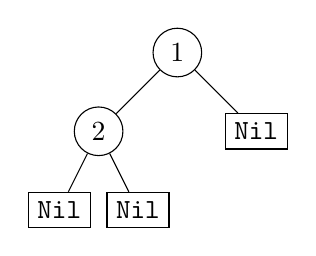
\begin{tikzpicture}
            \node[draw,circle] (A) at (0,0) {$1$};
            \node[draw,circle] (B) at (-1,-1) {$2$};
            \node[draw,rectangle] (C) at (1,-1) {\texttt{Nil}};
            \node[draw,rectangle] (D) at (-1.5,-2) {\texttt{Nil}};
            \node[draw,rectangle] (E) at (-0.5,-2) {\texttt{Nil}};
            \draw (A) -- (B) -- (D);
            \draw (A) -- (C);
            \draw (B) -- (E);
        \end{tikzpicture}
    \end{center}
    nous allons calculer son nombre de n\oe uds, en utilisant la fonction définie dans l'exercice précédent, dont on peut exprimer les règles d'induction de la façon suivante : 
    \begin{center}
        \begin{prooftree}
            \infer0{|\texttt{Nil}| = 0}
        \end{prooftree}
        \qquad
        \begin{prooftree}
            \hypo{|g| = k}
            \hypo{|d| = k'}
            \infer2{|\texttt{Node}(e,g,d)| = 1 + k + k'}
        \end{prooftree}
    \end{center}

    La dérivation est donc :
    \begin{center}
        \begin{prooftree}
            \infer0{|\texttt{Nil}| = 0}
            \infer0{|\texttt{Nil}| = 0}
            \infer2{|\texttt{Node}(2,\texttt{Nil},\texttt{Nil})| = 1 }
            \infer0{|\texttt{Nil}| = 0}
            \infer2{|A| = 2}
        \end{prooftree}
    \end{center}
\end{expl}


\begin{exo}
    Défnir les règles d'induction de la fonction $|-|$ sur les listes, associant à une liste sa longueur. \'Ecrire l'arbre de dérivation du calcul de $|[a,b,c]|$.
\end{exo}



\subsection{Relation inductive}

Intéressons-nous désormais aux relations entre objets inductifs. Comme précédemment, nous utiliserons des règles d'induction pour les définir (puisqu'une relation $\mathcal R$ peut être vue comme une fonction dans $\{0,1\}$), mais nous distinguerons deux types de prémisses : les prémisses du système formel et les prémisses \og meta\fg{}. Les premières sont celles qui interviennent directement dans les constructeurs de notre ensemble inductif, tandis que les deuxièmes sont des conditions que l'on peut dire extérieures à notre formalisme. Nous écrirons à côté de la règle les prémisses non syntaxiques (celles qui n'appartiennent pas au système formel). Attention cependant : nous nommerons souvent nos règles en donnant leur nom à droite de la barre, il faudra donc comprendre lorsqu'il y a une condition écrite à droite qu'elle est une prémisse non syntaxique, et lorsqu'il y a seulement un nom (par exemple $\to_e$) que c'est le nom de la règle.

\begin{expl}
    Nous allons définir le prédicat $P_k$ sur $\texttt{List}(\mathbb N)$ signifiant qu'une liste d'entiers possède un certain élément $k$ :
    \begin{center}\begin{prooftree}
        \hypo{}
        \infer1[$x = k$]{P_k(\texttt{cons}(x,l))}
    \end{prooftree}
    \qquad
    \begin{prooftree}
        \hypo{P_k(l)}
        \infer1{P_k(\texttt{cons}(x,l))}
    \end{prooftree}
    \end{center}
\end{expl}

\begin{exo}
    Montrer que $P_2([5,3,4,2,1,9])$ par un arbre de dérivation.
\end{exo}

\begin{rmk}
    On peut aussi définir des relations inductives mutuelles, par exemple un prédicat \og être pair\fg{} faisant appel à un prédicat \og être impair\fg{} faisant lui-même appel au premier prédicat (les deux ayant un cas de base), mais nous ne traiterons pas ce genre d'extension ici.
\end{rmk}

Donnons une définition de relation donnée par induction, car c'est un cas particulier qui nous sera utile.

\begin{defi}[Relation inductive]
    Soient $E,F$ deux ensembles. Soit un triplet $\langle C,\alpha,(D_c)_{c\in C}\rangle$ où $\alpha : C\to\nat, D_c : (E\times F)^{\alpha(c)}\to E\times F$ et $C$ est un ensemble. On dit que la relation $\mathcal R$ est définie par induction par ce triplet si $\mathcal R$ est la plus petite relation telle que pour tout $c\in C$, si pour tout $i \in\{0,\ldots,\alpha(c)\}, \mathcal R \langle x_i,y_i\rangle$ alors $\mathcal R(D_c(\langle x_1,y_1\rangle,\ldots,\langle x_{\alpha(c)},y_{\alpha(c)}\rangle))$. On note en général le triplet de la façon suivante : pour chaque $c\in C$, on écrit une règle de la forme
    \begin{center}
        \begin{prooftree}
            \hypo{\mathcal R(x_1,y_1)}
            \hypo{\mathcal R(x_2,y_2)}
            \hypo{\ldots}
            \hypo{\mathcal R(x_{\alpha(c)},y_{\alpha(c)})}
            \infer4[$c$]{\mathcal  R(D_c(\langle x_1,y_1\rangle,\ldots,\langle x_{\alpha(c)},y_{\alpha(c)}\rangle))}
        \end{prooftree}
    \end{center} avec $x_i,y_i$ non spécifiés, qu'il faut alors considérer comme quantifiée sur respectivement tout $E$ et tout $F$.
\end{defi}

\begin{exo}
    Montrer que si deux propositions sont stables par les règles définissant une relation inductive, alors l'intersection de ces propositions est aussi stable par ces règles. En déduire que la relation $\mathcal R$ définie par induction précédemment est l'intersection des propositions stables par les règles.
\end{exo}

\begin{exo}
    Montrer qu'une relation définie par induction par un ensemble de règles $\langle C,\alpha,(D_c)\rangle$ est non vide si et seulement s'il existe $c\in C$ tel que $\alpha(c) = 0$.
\end{exo}

\begin{rmk}
    Il arrivera que l'on écrive une règle dont les prémisses contiennent une ou des conditions qui ne sont pas de la forme $\mathcal R(x,y)$. Dans ce cas on peut considérer que l'on ajoute une règle de construction inductive pour chaque élément vérifiant cette prémisse et que le reste de la règle est paramétré par cet élément.
\end{rmk}

Nous pouvons maintenant réécrire notre théorème d'induction structurelle avec le formalisme des règles d'induction :

\begin{cor}[Preuve par induction]
    Soit une relation $\mathcal R$ entre deux ensembles $E,F$ générée par un ensemble de règles d'induction. Alors pour tout prédicat $P$ sur $E\times F$, pour montrer que $\mathcal R \subseteq P$ il suffit de montrer, pour chaque règle $c,\alpha(c),D_c$ définissant $\mathcal R$ la propriété suivante : pour tout $(x_1,\ldots,x_{\alpha(c)})\in P^{\alpha(c)}, P(D_c(x_1,\ldots,x_{\alpha(c)}))$, ce qui revient à montrer :
    \begin{center}
        \begin{prooftree}
            \hypo{P(x_1)}
            \hypo{P(x_2)}
            \hypo{\ldots}
            \hypo{P(x_{\alpha(c)})}
            \infer4[$c$]{P(D_c(x_1,\ldots,x_{\alpha(c)}))}
        \end{prooftree}
    \end{center}
\end{cor}

\begin{proof}
    C'est une conséquence directe du fait que $\mathcal R$ est définie comme la plus petite relation possédant cette propriété.
\end{proof}



\section{Définition des propositions}

Cette section vise à présenter les propositions, que nous introduirons comme des objets syntaxiques. La façon de séparer les propositions de leur interprétation (par exemple de dire que $\forall x. x = x$ n'est pas le même objet que $\top$) est une démarche qui se révélera fructueuse pour pouvoir trouver le bon formalisme pour parler de preuves et de valeur de vérité. On peut voir cela comme un analogue à la distinction entre un polynôme formel et une fonction polynomiale : le premier permet d'étudier de façon plus systématique le deuxième.

La première approche que nous aurons sera celle du calcul des propositions : on peut considérer une proposition (dans son sens intuitif) comme une phrase portant sur des objets mathématiques, par exemple avec la proposition $1 = 1$, auxquelles on associe des mots de liaison, comme $(1 = 1) \lor (0 = 1)$ indiquant que $1=1$ ou $0=1$. Cependant, on peut s'abstraire des prédicats de la forme $1=1$ et remplacer ceux-ci par une variable booléenne : une variable $x$ pouvant valoir $1$ (si elle représente une proposition atomique vraie) ou $0$ (si elle est fausse). Dans un second temps seulement, nous verrons le calcul des prédicats, permettant de parler plus précisément de ces propositions atomiques.

\subsection{Calcul des propositions}

\begin{defi}[Proposition]
    Soit un ensemble infini (dénombrable) de variables booléennes $\VV$ que nous noterons $x_1,x_2,\ldots$, nous définissons l'ensemble des propositions $\Prop$ par la grammaire suivante : $$ P,Q ::= x_i \mid \top\mid \bot \mid (P\to Q) \mid (P \lor Q) \mid (P\land Q)\mid (\lnot P)$$ où $\top$ et $\bot$ sont deux propositions atomiques constantes (appelées \og vrai\fg{} et \og absurde\fg{}).
\end{defi}

\begin{rmk}
    Un constructeur de cette grammaire est aussi appelé connecteur logique.
\end{rmk}

\begin{expl}
    Voici quelques propositions :
    \begin{itemize}[label=$\bullet$]
        \item $\top$
        \item $((\top \land (\lnot x_1))\lor (x_2\to x_3))$
    \end{itemize}
\end{expl}

\begin{rmk}
    Nous simplifierons l'écriture en rendant $\lnot$ le constructeur le plus prioritaire, $\lor$ et $\land$ prioritaire sur $\to$ et $\land$ prioritaire sur $\lor$ (le tout pour omettre un maximum de parenthèses). Par exemple la dernière proposition donnée en exemple peut se réécrire $\top\land \lnot x_1 \lor (x_2\to x_3)$. Enfin, l'opération $\to$ sera associative à droite : $x_0 \to x_1 \to x_2$ se lira $x_0 \to (x_1\to x_2)$.
\end{rmk}

Nous avons déjà une intuition assez naturelle de ce que veut dire chaque constructeur : par exemple, $P\land Q$ est vraie exactement lorsque $P$ et $Q$ à la fois sont vraies. Cette idée intuitive peut se formaliser par ce que l'on appelle des tables de vérité, représentant pour un connecteur la valeur de la proposition qu'il construit en fonction de la valeur de vérité de ses entrée. Voici les tables de vérité des différents connecteurs logiques :

{\begin{figure}[htb]
\centering
\begin{tabular}{|c|c|}
    \hline
     $P$ & $\lnot P$ \\ \hline\hline
     0 & 1 \\ \hline
     1 & 0 \\ \hline
\end{tabular}
\quad
\begin{tabular}{|c|c|c|}
    \hline
     $P$ & $Q$ & $P\to Q$ \\ \hline\hline
     0 & 0 & 1\\ \hline
     0 & 1 & 1\\ \hline
     1 & 0 & 0\\ \hline
     1 & 1 & 1\\ \hline
\end{tabular}
\quad
\begin{tabular}{|c|c|c|}
    \hline
     $P$ & $Q$ & $P\lor Q$  \\ \hline\hline
     0 & 0 & 0 \\ \hline
     0 & 1 & 1 \\ \hline
     1 & 0 & 1 \\ \hline
     1 & 1 & 1\\ \hline
\end{tabular}
\quad
\begin{tabular}{|c|c|c|}
    \hline
     $P$ & $Q$ & $P\land Q$ \\ \hline\hline
     0 & 0 & 0 \\ \hline
     0 & 1 & 0 \\ \hline
     1 & 0 & 0 \\ \hline
     1 & 1 & 1 \\ \hline
\end{tabular}
\caption{Tables de vérité}
\end{figure}}
\newpage

On peut alors essayer de donner une table de vérité pour n'importe quelle formule propositionnelle, mais les tables de vérité ont plusieurs inconvénients : elles sont longues à faire et elles sont difficiles à étudier mathématiquement. Nous leur préférerons donc la notion de valuation, que nous allons maintenant introduire.

\begin{defi}[Valuation]
    Soit une fonction $\nu : \VV \to \{0,1\}$ (qui à une variable associe si elle est vraie ou non), nous allons étendre par induction $\nu$ en une fonction $\nu^*:\Prop \to \{0,1\}$ par les règles suivantes :
    \begin{center}
        \begin{prooftree}
            \infer0[$\top$]{\nu^*(\top)=1}
        \end{prooftree}
        \quad
        \begin{prooftree}
            \infer0[$\bot$]{\nu^*(\bot)=0}
        \end{prooftree}
        \quad
        \begin{prooftree}
            \infer0[Ax]{\nu^*(x_i) = \nu(x_i)}
        \end{prooftree}
        \\
        \vspace{0.5cm}
        \begin{prooftree}
            \hypo{\nu^*(P) = b}
            \infer1[$\lnot$]{\nu^*(\lnot P) = 1 - b}
        \end{prooftree}
        \quad
        \begin{prooftree}
            \hypo{\nu^*(P) = b_1}
            \hypo{\nu^*(Q) = b_2}
            \infer2[$\to$]{\nu^*(P\to Q) = 1-b_1+b_1\times b_2}
        \end{prooftree}\\
        \vspace{0.5cm}
        \begin{prooftree}
            \hypo{\nu^*(P) = b_1}
            \hypo{\nu^*(Q) = b_2}
            \infer2[$\lor$]{\nu^*(P\lor Q) = b_1 + b_2 - b_1\times b_2}
        \end{prooftree}
        \quad
        \begin{prooftree}
            \hypo{\nu^*(P) = b_1}
            \hypo{\nu^*(Q) = b_2}
            \infer2[$\land$]{\nu^*(P\land Q) = b_1\times b_2}
        \end{prooftree}
    \end{center}
\end{defi}

\begin{rmk}
    Les opérations utilisées pour les valuations de $P\to Q$ et $P\lor Q$ sont un peu longues, mais elles correspondent simplement à leur table de vérité.
\end{rmk}

\begin{exo}
    Montrer par une dérivation que chaque table de vérité est vérifiée avec notre définition de $\nu^*$.
\end{exo}

\begin{exo}
    Montrer que deux valuations $\nu,\nu'$ donnent la même valeur sur une proposition $P$ si pour toute variable $x_i$ intervenant dans $P$, $\nu(x_i)=\nu'(x_i)$.
\end{exo}

On peut donc se restreindre aux valuations $\nu$ partielles, c'est-à-dire n'associant qu'un nombre fini de valeurs à l'ensemble $\VV$, dont le domaine contient les variables intervenant dans une proposition $P$, pour évaluer $P$.

\begin{expl}
    Soit la proposition $P := x_0\lor x_1 \to x_2$, et la valuation $$\nu : x_0 \mapsto 0, x_1 \mapsto 1, x_2 \mapsto 0$$ on peut alors calculer $\nu^*(P)$ :
    \begin{center}
        \begin{prooftree}
            \infer0[Ax]{\nu^*(x_0)=0}
            \infer0[Ax]{\nu^*(x_1)=1}
            \infer2[$\lor$]{\nu^*(x_0\lor x_1) = 1}
            \infer0[Ax]{\nu^*(x_2)=0}
            \infer2[$\to$]{\nu^*(x_0\lor x_1 \to x_2) = 0}
        \end{prooftree}
    \end{center}
\end{expl}

Si l'on considère que $1$ signifie que la proposition est vraie et que $0$ signifie que la proposition est fausse, on peut donc dire qu'une proposition est vraie pour une certaine valuation. 

\begin{defi}[Modèle d'une proposition]
    Soit $\nu$ une valuation. On dit que $P$ est vraie (ou satisfaite) pour la valuation $\nu$, ou encore que $\nu$ est modèle de $P$, et on note $\nu\models P$, si $\nu^*(P) = 1$.
\end{defi}

\begin{defi}[Tautologie]
    On dit que $P$ est une tautologie si pour toute valuation $\nu$, $\nu^*\models P$.
\end{defi}

Par la suite, on confondra directement $\nu$ et $\nu^*$.

\subsection{Satisfiabilité et compacité}

\'Etendons maintenant notre notion de vérité pour un ensemble de propositions :

\begin{defi}[Satisfiabilité]
    On dit qu'une formule $P$ est satisfiable s'il existe une valuation $\nu$ telle que $\nu\models P$.

    Si $\mathbf{P}\subseteq \Prop$ est un ensemble de proposition, alors on dit que $\mathbf{P}$ est satisfiable s'il existe une valuation $\nu$ telle que pour tout $P\in\mathbf{P}$, $\nu\models P$. On note alors $\nu\models \textbf{P}$.
\end{defi}

\begin{rmk}
    Cette digression est hors du cadre de ce document, mais le problème de trouver, étant donnée une proposition, si elle est satisfiable, est un problème dit NP-complet. Il est historiquement le premier problème démontré comme étant NP-complet et revêt en ce sens une importance primordiale en théorie de la complexité algorithmique.
\end{rmk}

Donnons aussi la définition d'un ensemble contradictoire :

\begin{defi}[Ensemble contradictoire]
    Un ensemble $\mathbf P\subseteq \mathcal P$ (potentiellement infini) est contradictoire s'il n'existe pas de valuation $\nu$ telle que $\nu\models \mathbf P$.
\end{defi}

Le calcul des propositions n'est malheureusement pas le plus pertinent, car il manque à ce système deux éléments essentiels : pouvoir s'appliquer à des objets mathématiques et pouvoir introduire des quantifications. Nous nous contenterons donc de donner un théorème central de la logique : le théorème de compacité.

\begin{defi}[Ensemble finiment satisfiable, contradictoire]
    Soit $\mathbf{P}$ un ensemble (infini) de propositions, on dit que $\mathbf{P}$ est finiment satisfiable si pour toute partie finie $P\subseteq_{\mathrm{fin}}\mathbf P$, $P$ est satisfiable.
    
    De même, $\mathbf P$ est dite finiment contradictoire s'il existe une partie finie de $\mathbf P$ qui est contradictoire.
\end{defi}

\begin{them}[Compacité de la logique propositionnelle]
    Soit $\mathbf P$ un ensemble de propositions. Alors $\mathbf P$ est satisfiable si et seulement si $\mathbf P$ est finiment satisfiable.
\end{them}

\begin{proof}
    Il est évident qu'un ensemble satisfiable est finiment satisfiable, le théorème tient bien sûr dans le sens réciproque.

    Soit un ensemble de propositions $\mathbf P$. Nous allons définir une suite $(\varepsilon_n)$ qui définira notre valuation par $\nu(x_n)=\varepsilon_n$. Cette construction se fera par induction :
    \begin{itemize}[label=$\bullet$]
        \item Tout d'abord, deux cas sont possibles :
        \begin{enumerate}
            \item\label{cas1} pour tout sous-ensemble fini $B$, il existe une valuation $\delta$ satisfiant $B$ et telle que $\delta(x_0)=0$ : dans ce cas on définit $\varepsilon_0 = 0$.
            \item\label{cas2} il existe un sous-ensemble fini $B_0$ tel que pour toute valuation $\delta$ satisfiant $B_0$, $\delta(x_0)=1$ : dans ce cas on définit $\varepsilon_0 = 1$.
        \end{enumerate} 
        \item Montrons l'initialisation de la propriété \og il existe une suite $\varepsilon_0,\ldots,\varepsilon_n$ telle que pour tout sous-ensemble $B$ il existe un valuation $\delta$ satisfaisant $B$ et telle que $\delta(x_i)=\varepsilon_i$\fg{} : dans le cas \ref{cas1}, le résultat est direct. Dans le cas \ref{cas2}, alors pour une partie finie $B$ on considère $B\cup B_0$ : si $\delta\models B\cup B_0$ alors $\delta\models B_0$ donc $\delta(x_0)=1$ et $\delta\models B$, donc notre hypothèse est vérifiée.
        \item Supposons qu'il existe une suite $\varepsilon_0,\ldots,\varepsilon_n$ vérifiant les conditions énoncées, alors on peut encore séparer deux cas :
        \begin{enumerate}
            \item pour toute partie finie $B$ il existe une valuation $\delta\models B$ telle que $\delta(x_i)=\varepsilon_i$ pour $i\leq n$, on a aussi $\delta(x_{n+1})=0$.
            \item il existe une partie finie $B_{n+1}$ telle que pour toute valuation $\delta\models B$ telle que $\delta(x_i) =\varepsilon_i$ pour $i\leq n$, on a $\delta(x_{n+1})=1$.
        \end{enumerate}
        Dans le premier cas, on définit $\varepsilon_{n+1}=0$ et l'hérédité est vérifiée, et dans le deuxième cas on définir $\varepsilon_{n+1}=1$ et alors pour $B$ une partie finie, il existe $\delta\models B \cup B_{n+1}$ avec $\delta(x_i)=\varepsilon_i$ pour $i\leq n$, et comme $\delta\models B_{n+1}$ on en déduit qu'il existe $\delta\models B$ avec $\delta(x_i) =\varepsilon_i$ pour $i\leq n+1$.
    \end{itemize}

    Ainsi, par récurrence, nous avons défini la valuation $\nu : x_i \mapsto \varepsilon_i$ qui satisfait toute proposition de $\mathbf P$.
\end{proof}

\begin{exo}[Formulation équivalente du théorème de compacité]
    Montrer que le théorème de compacité équivaut au théorème suivant : tout ensemble est contradictoire si et seulement s'il est finiment contradictoire.
\end{exo}


\section{Liens entre syntaxe et sémantique}

Nous avons défini, dans notre syntaxe, le connecteur $\to$, qui se traduit en général par \og $P\to Q$ signifie que $Q$ est une conséquence logique de $P$\fg{}. Cependant, ce connecteur ne possède pas de sens en lui-même : il n'a de sens qu'à travers notre règle d'induction pour la définition de $\nu^*$, car c'est bien le comportement des connecteurs vis à vis des valuations qui détermine le sens de ces connecteurs (plus précisément : le sens est donné par les valuations, c'est pour cela qu'on considère que celles-ci sont un aspect sémantique de notre logique, là où les suites de symboles que sont les propositions sont purement syntaxiques). Cependant, de par la forme des propositions, on peut établir un système qui, sans utiliser de valuations, va pouvoir exprimer des notions de conséquence (entre autres choses).

\begin{defi}[Conséquence sémantique]
    Soit $\mathbf P\subseteq\mathcal P$ un ensemble de proposition et $P$ une proposition, on dit que $P$ est conséquence sémantique de $\mathbf P$ si pour toute valuation $\nu\models\mathbf P$, on a $\nu\models P$. 
\end{defi}

\begin{expl}
    Il est évident que si $P\in\mathbf P$, alors $P$ est conséquence sémantique de $\mathbf P$. On peut aussi montrer que si $P\in\mathbf P$ et $Q\in\mathbf P$ alors $P\land Q$ est conséquence sémantique de $\mathbf P$.
\end{expl}

\begin{exo}
    Montrer qu'une formulation équivalente du théorème de compacité est la suivante : une proposition $P$ est conséquence sémantique d'un ensemble de propositions $\mathbf P$ si et seulement si elle est conséquence sémantique d'une partie finie de $\mathbf P$.
\end{exo}

\subsection{Déduction naturelle avec présentation en séquents}

A partir de nos exemples se dessine un schéma de règles assez naturel : pour un ensemble de propositions, on peut directement dériver des propositions qui en sont des conséquences sémantiques, sans avoir à raisonner réellement sur les valuations. Nous allons donc définir un système syntaxique appelé déduction naturelle permettant de formaliser cette idée.

\begin{defi}[Séquent en déduction naturelle]
    Soit $\Gamma$ un ensemble de propositions (présenté sous forme de liste) et $P$ une propositions, on note $\Gamma\vdash P$, et on lit \og gamma thèse $P$\fg{} le séquent exprimant que $P$ peut se déduire des hypothèses $\Gamma$. Ceci constitue une relation inductive dont les règles de constructions sont précisées dans la figure \ref{fig:deducnat} ci-dessous.
\end{defi}

\begin{figure}[htb]
    \centering
    \rule{17cm}{0.5pt}\\
    \vspace{0.5cm}
    \begin{prooftree}
        \infer0[$\top_\mathrm{i}$]{\Gamma\vdash \top}
    \end{prooftree}
    \quad
    \begin{prooftree}
        \infer0[Ax]{\Gamma,P\vdash P}
    \end{prooftree}
    \quad
    \begin{prooftree}
        \hypo{\Gamma,P\vdash Q}
        \infer1[$\to_\mathrm i$]{\Gamma\vdash P\to Q}
    \end{prooftree}
    \quad
    \begin{prooftree}
        \hypo{\Gamma\vdash P\to Q}
        \hypo{\Gamma\vdash P}
        \infer2[$\to_\mathrm e$]{\Gamma\vdash Q}
    \end{prooftree}
    \\
    \vspace{0.5cm}
    \begin{prooftree}
        \hypo{\Gamma\vdash P}
        \hypo{\Gamma\vdash Q}
        \infer2[$\land_\mathrm i$]{\Gamma\vdash P\land Q}
    \end{prooftree}
    \quad
    \begin{prooftree}
        \hypo{\Gamma\vdash P\land Q}
        \infer1[$\land_\mathrm e^\mathrm g$]{\Gamma\vdash P}
    \end{prooftree}
    \quad
    \begin{prooftree}
        \hypo{\Gamma\vdash P\land Q}
        \infer1[$\land_\mathrm e^\mathrm d$]{\Gamma\vdash Q}
    \end{prooftree}
    \\
    \vspace{0.5cm}
    \begin{prooftree}
        \hypo{\Gamma\vdash P}
        \infer1[$\lor_\mathrm i^\mathrm g$]{\Gamma\vdash P \lor Q}
    \end{prooftree}
    \quad
    \begin{prooftree}
        \hypo{\Gamma\vdash Q}
        \infer1[$\lor_\mathrm i^\mathrm d$]{\Gamma\vdash P \lor Q}
    \end{prooftree}
    \quad
    \begin{prooftree}
        \hypo{\Gamma\vdash P \lor Q}
        \hypo{\Gamma,P\vdash C}
        \hypo{\Gamma,Q\vdash C}
        \infer3[$\lor_\mathrm e$]{\Gamma\vdash C}
    \end{prooftree}
    \\
    \vspace{0.5cm}
    \begin{prooftree}
        \hypo{\Gamma,A\vdash \bot}
        \infer1[$\lnot_\mathrm i$]{\Gamma\vdash \lnot A}
    \end{prooftree}
    \quad
    \begin{prooftree}
        \hypo{\Gamma\vdash A}
        \hypo{\Gamma\vdash \lnot A}
        \infer2[$\lnot_\mathrm e$]{\Gamma\vdash \bot}
    \end{prooftree}
    \quad
    \begin{prooftree}
        \hypo{\Gamma,\lnot A\vdash \bot}
        \infer1[$\bot_\mathrm c$]{\Gamma\vdash A}
    \end{prooftree}
    \\
    \vspace{0.5cm}
    \rule{17cm}{0.5pt}
    \caption{Règles de la déduction naturelle}
    \label{fig:deducnat}
\end{figure}

\begin{rmk}
    On appelle un arbre de preuve une dérivation, à partir de ces règles, d'un séquent.

    Si $\Gamma=\varnothing$, on notera directement $\vdash P$.
\end{rmk}

\begin{expl}
Voici un exemple de dérivation de $P\to P$ :
\begin{center}
    \begin{prooftree}
        \infer0[Ax]{P\vdash P}
        \infer1[$\to_\mathrm i$]{\vdash P \to P}
    \end{prooftree}
\end{center}
\end{expl}

\begin{exo}
    Pour chaque proposition, construire un arbre de preuve :
    \begin{itemize}[label=$\bullet$]
        \item $\vdash P \to Q \to P$
        \item $\vdash (P \to Q \to R) \to (P \to Q) \to P \to R$
        \item $(P\lor Q)\land R\vdash (P\land R)\lor (Q\land R)$
        \item $\lnot\lnot A \to A$
        \item $\lnot A \lor A$
    \end{itemize}
\end{exo}

\begin{exo}[Principe d'explosion]
    Une règle importante en logique, nommée \textit{ex falso quodlibet}, stipule que si l'on prouve $\bot$ (la formule fausse) alors on peut prouver n'importe quoi, elle s'écrit \begin{center}
        \begin{prooftree}
            \hypo{\Gamma\vdash \bot}
            \infer1[$\bot_\mathrm i$]{\Gamma\vdash A}
        \end{prooftree}
    \end{center}
    Montrer que $\bot_\mathrm i$ est dérivable, c'est-à-dire que l'on peut construire un arbre partant de la prémisse de la règle pour arriver à sa conclusion (la lettre i pour désigner cette règle fait référence à l'intuitionnisme, car cette règle remplace $\bot_\mathrm c$, l'absurde classique, en logique intuitionniste).
\end{exo}

Nous pouvons remarquer que chaque règle d'induction correspond à une règle logique évidente :
\begin{itemize}[label=$\bullet$]
    \item La règle $\top_\mathrm i$ dit simplement que l'on peut toujours déduire la formule vraie.
    \item La règle Ax dit que l'on peut déduire $P$ directement si l'on a fait l'hypothèse $P$.
    \item La règle $\to_\mathrm i$ dit que pour montrer $P\to Q$ il suffit de supposer $P$ pour montrer $Q$.
    \item La règle $\to_\mathrm e$, aussi appelée \textit{modus ponens}, dit que si l'on a prouvé $P\to Q$ et $P$, alors on peut en déduire $Q$.
    \item Les règles liées à $\lor$, $\land$ et $\lnot$ sont assez lisibles, à l'exception de $\lor_\mathrm e$ : elle correspond à la disjonction de cas. En effet, si l'on a prouvé $P\lor Q$, alors prouver $C$ revient à le prouver sous l'hypothèse $P$ et sous l'hypothèse $Q$.
    \item La règle $\bot_\mathrm c$, appelée raisonnement par l'absurde, permet de déduire $A$ du fait que $\lnot A$ mène à une contradiction.
\end{itemize}

L'exercice suivant est un résultat de structure de notre système, qui sera utile par la suite :

\begin{exo}[Affaiblissement]
    Montrer par induction que s'il existe une dérivation de $\Gamma\vdash P$ alors pour toute proposition $A$, il existe une dérivation de $\Gamma,A\vdash P$ (ceci signifie que si l'on a prouvé un résultat, on peut encore le prouver en rajoutant des hypothèses).
\end{exo}

\begin{exo}[Codage de la négation]
    Montrer que le séquent suivant est dérivable : $$\vdash (\lnot P \to (P\to\bot))\land((P\to\bot)\to\lnot P)$$
\end{exo}

\subsection{Correction et complétude du calcul propositionnel}

Ces règles paraissent dont très convaincantes pour créer un formalisme robuste de raisonnement. Pourtant, ce ne sont que des règles formelles : des enchaînements de symboles qui n'ont \textit{a priori} pas de lien avec la sémantique de nos propositions. Heureusement, il existe une paire de théorème nous permettant d'établir l'équivalence entre la conséquence sémantique et la conséquence syntaxique (c'est-à-dire le fait de prouver $\Gamma\vdash P$).

\begin{them}[Correction du calcul propositionnel]
    Si $\Gamma\vdash P$ pour $\Gamma$ un ensemble de propositions, alors $P$ est conséquence sémantique de $\Gamma$, i.e. pour toute valuation $\nu$, si $\nu\models\Gamma$ alors $\nu\models P$.
\end{them}

\begin{proof}
    La preuve se fait par induction sur $\Gamma\vdash P$, il suffit donc de montrer que pour chaque règle, si le théorème est vrai pour ses prémisses, alors il est vrai pour sa conclusion. Nous laissons en exercice au lecteur le traitement de la plupart des règles, mais donnerons le traitement de deux règles pour l'exemple :
    \begin{itemize}[label=$\bullet$]
        \item Cas de $\to_\mathrm e$ : supposons que $\Gamma\vdash P\to Q$ et $\Gamma\vdash P$, et de plus que cela $P\to Q$ et $P$ sont conséquences sémantiques de $\Gamma$ (par hypothèse d'induction), montrons qu'alors $Q$ est conséquence sémantique de $\Gamma$. Soit $\nu$ satisfaisant $\Gamma$, alors par hypothèse, $\nu(P) = 1$ et $\nu(P\to Q)=1$, or $\nu(P\to Q) = 1 - \nu(P)+\nu(P)\nu(Q)$ donc en simplifiant, on en déduit que $\nu(Q) = 1$ : donc $Q$ est conséquence sémantique de $\Gamma$.
        \item Cas de $\lor_\mathrm e$ : on suppose donc que $P\lor Q$ est conséquence sémantique de $\Gamma$, que $C$ est conséquence sémantique de $\Gamma,P$ et de $\Gamma,Q$, et on veut montrer que $C$ est conséquence sémantique de $\Gamma$. Soit $\nu$ satisfaisant $\Gamma$, alors $\nu(P\lor Q) = 1$, c'est-à-dire $\nu(P)+\nu(Q)-\nu(P)\nu(Q)=1$. Alors soit $\nu(P)=1$, soit $\nu(Q)=1$ (possiblement les deux). Supposons sans perte de généralité que $\nu(P)=1$ : cela signifie que $\nu$ satisfait $\Gamma,P$, donc comme $C$ est conséquence logique de $\Gamma,P$, $\nu(C)=1$. Donc $C$ est conséquence logique de $\Gamma$. 
    \end{itemize}
\end{proof}

\begin{exo}
    Montrer le théorème pour les autre règles d'induction.
\end{exo}

Ce théorème nous dit donc que ce qu'on prouve avec ces règles est correct. La question naturelle qui s'ensuit est \og peut-on prouver tout ce qui est vrai ?\fg{} Il se trouve que c'est le cas, c'est ce que montre le prochain théorème.

Pour préparer ce résultat, nous aurons besoin d'une suite de lemmes (le premier sera ici donné en exercice). Ces lemmes ont des preuves principalement techniques et il est conseillé pour le lecteur de ne pas s'attarder sur celles-ci.

\begin{exo}
    Montrer que $P$ est conséquence sémantique d'un ensemble fini de propositions $\Gamma$ si et seulement si $\left(\displaystyle{\bigwedge_{\gamma\in\Gamma}}\gamma \right)\to P$ est une tautologie. Où cette notation signifie que l'on considère la conjonction (connecteur \og et\fg{}) sur toutes les formules de $\Gamma$.
\end{exo}

Nous allons construire, pour une valuation $\nu$, une proposition permettant de représenter, en quelque sorte, $\nu$. La preuve se basera sur le fait que $\nu\models P$ pourra s'interpréter comme $\vdash \nu\to P$.

\begin{lem}
    Soit $P$ une proposition et $\nu$ une valuation sur les variables de $P$, on note $V(\nu)$ une proposition correspondant à une conjonction contenant toutes les propositions $x_i$ telles que $\nu(x_i)=1$ et les négations des propositions $x_j$ telles que $\nu(x_j) = 0$. Par exemple pour $\nu(x_0)=1,\nu(x_1)=0$ on a au moins $V(\nu) = x_0\land \lnot x_1$. Alors :
    \begin{itemize}[label=$\bullet$]
        \item soit $\nu(P) = 1$ et alors $V(\nu) \vdash P$
        \item soit $\nu(P) = 0$ et alors $V(\nu) \vdash \lnot P$.
    \end{itemize}
\end{lem}

\begin{proof}
    Procédons par induction sur $P$ :
    \begin{itemize}[label=$\bullet$]
        \item Les cas $\top$ et $\bot$ sont évidents, puisqu'ils ne font pas intervenir de variables.
        \item Cas $x_i$ : soit $V(\nu)$ avec $\nu$ une valuation sur $x_i$. Supposons que $\nu(x_i)=1$. Alors \begin{center}
            \begin{prooftree}
                \infer0[Ax]{V(\nu)\vdash V(\nu)}
                \infer1[$\land_\mathrm e$]{V(\nu)\vdash x_i}
            \end{prooftree}
        \end{center} où l'on note $\land_\mathrm e$ pour choisir le $x_i$ précis dans $V(\nu)$ (on peut se convaincre qu'une suite finie d'applications de $\land_\mathrm e$ permet de faire ceci). La preuve est la même si $\nu(x_i) = 0$ (on obtiendra simplement $\lnot x_i$ à la place).
        \item Cas $\lor$ : soit $\nu$ une valuation contenant les variables de $P$ et de $Q$, et $V(\nu)$ une proposition associée à $\nu$. Quatre cas peuvent alors arriver, mais nous ne traiterons que deux d'entre eux (le lectuer assidu vérifiera les autres) : si $\nu(P)=1$ et $\nu(Q)=0$ (et donc que $\nu(P\lor Q) = 1$) alors on sait que $V(\nu)\vdash P$ et $V(\nu)\vdash \lnot Q$. On construit alors :
        \begin{center}
            \begin{prooftree}
                \hypo{V(\nu)\vdash P}
                \infer1[$\lor_\mathrm i$]{V(\nu)\vdash P\lor Q}
            \end{prooftree}
        \end{center}
        Si $\nu(P)=\nu(Q)=0$ alors $V(\nu)\vdash \lnot P$, $V(\nu)\vdash \lnot Q$ et on veut montrer que $V(\nu)\vdash \lnot (P\lor Q)$ :
        \begin{center}
        \scalebox{0.7}{
            \begin{prooftree}
                \infer0[Ax]{V(\nu),P\lor Q\vdash P\lor Q}
                \hypo{V(\nu),P\lor Q,P\vdash \lnot P}
                \infer0[Ax]{V(\nu),P\lor Q,P\vdash P}
                \infer2[$\lnot_\mathrm e$]{V(\nu),P\lor Q,P\vdash \bot}
                \hypo{V(\nu),P\lor Q,Q\vdash \lnot Q}
                \infer0[Ax]{V(\nu),P\lor Q,Q\vdash Q}
                \infer2[$\lnot_\mathrm e$]{V(\nu),P\lor Q,Q\vdash \bot}
                \infer3[$\lor_\mathrm e$]{V(\nu),P\lor Q\vdash\bot}
                \infer1[$\lnot_\mathrm i$]{V(\nu)\vdash \lnot (P\lor Q)}
            \end{prooftree}
        }
        \end{center}
        \item Cas $\land$ : soit $\nu$ une valuation contenant les variables de $P$ et de $Q$ et $V(\nu)$ une proposition associée à $\nu$. Là encore, quatre cas sont possibles. Si $\nu(P)=\nu(Q)=0$ alors par hypothèse d'induction $V(\nu)\vdash \lnot P$, $V(\nu)\vdash \lnot Q$, et alors :
        \begin{center}
            \begin{prooftree}
                \hypo{V(\nu),P\land Q\vdash \lnot P}
                \infer0[Ax]{V(\nu),P\land Q\vdash P\land Q}
                \infer1[$\land_\mathrm e^\mathrm g$]{V(\nu),P\land Q\vdash P}
                \infer2[$\lnot_\mathrm e$]{V(\nu),P\land Q\vdash \bot}
                \infer1[$\lnot_\mathrm i$]{V(\nu)\vdash \lnot(P\land Q)}
            \end{prooftree} 
        \end{center}
        Si $\nu(P)=0$ et $\nu(Q) = 1$, remarquons que l'arbre plus haut est encore parfaitement utilisable puisque $\nu(P\land Q) = 0$. De même en inversant les rôles de $P$ et $Q$, on peut prouver le cas où $\nu(P)=1$ et $\nu(Q)=0$. Enfin, si $\nu(P)=\nu(Q)=1$ :
        \begin{center}
            \begin{prooftree}
                \hypo{V(\nu)\vdash P}
                \hypo{V(\nu)\vdash Q}
                \infer2[$\land_\mathrm i$]{V(\nu)\vdash P\land Q}
            \end{prooftree}
        \end{center}
        \item Cas $\lnot$ : soit $\nu$ une valuation contenant les variables de $P$, et $V(\nu)$ une proposition associée. Si $\nu(P) = 1$ alors $\nu(\lnot(P))=0$, on veut donc montrer qu'à partir de $V(\nu)\vdash P$ on peut déduire $V(\nu)\vdash \lnot\lnot P$ :
        \begin{center}
            \begin{prooftree}
                \hypo{V(\nu),\lnot P\vdash P}
                \infer0[Ax]{V(\nu),\lnot P\vdash \lnot P}
                \infer2[$\lnot_\mathrm e$]{V(\nu),\lnot P\vdash \bot}
                \infer1[$\lnot_\mathrm i$]{V(\nu)\vdash \lnot \lnot P}
            \end{prooftree}
        \end{center}
        Si $\nu(P)=0$, alors on veut montrer qu'à partir de $V(\nu)\vdash \lnot P$ on peut en déduire que $V(\nu)\vdash \lnot P$, ce qui est évident.
        \item Cas $\to$ : soit $\nu$ une valuation contenant les variables de $P$ et $Q$, et $V(\nu)$ une proposition associée. Il reste encore quatre cas à traiter. Si $\nu(P)=\nu(Q)=0$, alors on veut montrer que $V(\nu)\vdash P\to Q$ à partir de $V(\nu)\vdash \lnot P$ et $V(\nu)\vdash \lnot Q$ :
        \begin{center}
            \begin{prooftree}
                \hypo{V(\nu),P\vdash \lnot P}
                \infer0[Ax]{V(\nu),P\vdash P}
                \infer2[$\lnot_\mathrm e$]{V(\nu),P\vdash\bot}
                \infer1[$\bot_\mathrm i$]{V(\nu),P\vdash Q}
                \infer1[$\to_\mathrm i$]{V(\nu)\vdash P\to Q}
            \end{prooftree}
        \end{center}
        Remarquons que nous n'avons, là encore, pas eu besoin d'utiliser l'hypothèse sur $Q$. On peut donc traiter avec le même arbre le cas où $\nu(P)=0$ et $\nu(Q)=1$. Si $\nu(P) = 1$ et $\nu(Q)=0$, il nous faut prouver $V(\nu)\vdash \lnot (P\to Q)$ avec les hypothèses $V(\nu)\vdash P$ et $V(\nu)\vdash \lnot Q$ :
        \begin{center}
            \begin{prooftree}
                \hypo{V(\nu),P\to Q\vdash \lnot Q}
                \hypo{V(\nu),P\to Q\vdash P}
                \infer0[Ax]{V(\nu),P\to Q\vdash P \to Q}
                \infer2[$\to_\mathrm e$]{V(\nu),P\to Q\vdash Q}
                \infer2[$\lnot_\mathrm e$]{V(\nu),P\to Q\vdash \bot}
                \infer1[$\lnot_\mathrm i$]{V(\nu)\vdash \lnot (P\to Q)}
            \end{prooftree}
        \end{center}
        Enfin, si $\nu(P)=\nu(Q)=1$, alors par $\to_\mathrm i$ on déduit de $V(\nu),P\vdash Q$ que $V(\nu)\vdash P\to Q$.
    \end{itemize}
\end{proof}

\begin{lem}
    Soit $P$ une proposition. Si $P$ est une tautologie, alors $\vdash P$.
\end{lem}

\begin{proof}
    Procédons par récurrence sur l'indice maximal des variables présentes dans $P$ :
    \begin{itemize}[label=$\bullet$]
        \item Si la seule variable apparaissant dans $P$ est $x_0$, alors comme $P$ est une tautologie et par le lemme précédent, on sait que $x_0\vdash P$ et $\lnot x_0\vdash P$, ce qui nous permet de déduire que $\vdash P$ (en utilisant un exercice précédent où l'on a montré que $\vdash A\lor\lnot A$) :
        \begin{center}
            \begin{prooftree}
                \hypo{\vdash x_0\lor\lnot x_0}
                \hypo{x_0\vdash P}
                \hypo{\lnot x_0\vdash P}
                \infer3[$\lor_\mathrm e$]{\vdash P}
            \end{prooftree}
        \end{center}
        \item Supposons que pour toute proposition faisant intervenir des variables jusqu'à $i$, être une tautologie implique d'être dérivable dans notre système. Soit alors une proposition $P$ faisant intervenir des variables jusqu'à $i+1$. Soit $\nu$ une valuation sur les $i$ premières variables. Comme $P$ est une tautologie, alors $P$ est satisfaite par $\nu'$ valant $\nu$ jusqu'à $x_i$ et $1$ en $x_{i+1}$, et par $\nu''$ valant $\nu$ jusqu'à $x_i$ et $0$ en $x_{i+1}$. On en déduit donc que $V(\nu')\vdash P$ et $V(\nu'')\vdash P$, soit $V(\nu)\land x_{i+1}\vdash P$ et $V(\nu)\land \lnot x_{i+1}\vdash P$. Par introductions successives de l'implication, on a alors $x_{i+1}\vdash V(\nu)\to P$ et $\lnot x_{i+1}\vdash V(\nu)\to P$, nous ramenant (en utilisant le même raisonnement que le cas précédent) à $\vdash V(\nu)\to P$, ce qui revient à $V(\nu)\vdash P$ qui est dérivable par le lemme précédent.
    \end{itemize}

    Donc par induction, $\vdash P$.
\end{proof}

\begin{rmk}
    Nous avons ici utilisé que si $P\land Q \vdash R$ alors $Q\vdash P\to R$. Ceci n'est pas une règle de à proprement parler, mais on peut prouver ce résultat par induction sur les arbres de preuve. Cela peut faire un exercice, mais il est surtout fastidieux et l'idée est principalement que l'on peut remplacer $P\land Q\vdash R$ par $P,Q\vdash R$ en remplaçant chaque utilisation de l'axiome pour $P$ ou pour $Q$ par un axiome pour $P\land Q$ puis une élimination du $\land$. Nous pouvons le statuer comme une sorte de meta-règle (qui nous permet de dire qu'un séquent est dérivable à partir d'un autre séquent qui est dérivable), qu'on appelle une règle admissible.
\end{rmk}

\begin{them}[Complétude du calcul propositionnel]
    Soit $\Gamma$ un ensemble de propositions et $P$ une proposition. Si $P$ est conséquence sémantique de $\Gamma$, i.e. pour toute valuation $\nu$, si $\nu\models\Gamma$ alors $\nu\models P$, alors $\Gamma\vdash P$.
\end{them}

\begin{proof}
    Sous nos hypothèses, avec le théorème de compacité, on peut considérer une partie finie $\Gamma_0\subseteq\Gamma$ telle que $P$ en est conséquence sémantique. On veut donc prouver que $\Gamma_0\vdash P$, ce qui revient à montrer que $\vdash \left(\displaystyle{\bigwedge_{\gamma\in\Gamma_0}}\gamma \right)\to P$, et la condition sémantique est équivalente à dire que $\left(\displaystyle{\bigwedge_{\gamma\in\Gamma_0}}\gamma \right)\to P$ est une tautologie. Nous n'avons donc à montrer que le résultat (plus faible) suivant : si $P$ est une tautologie, alors $\vdash P$ est dérivable. C'est justement le résultat du lemme précédent.
\end{proof}

\begin{exo}[\'Enoncé équivalent du théorème de complétude]
    Montrer que le théorème de complétude revient à l'énoncé suivant : si $\Gamma$ est contradictoire, alors $\Gamma\vdash \bot$.
\end{exo}

Nous savons maintenant qu'avec notre système de calcul, la preuve syntaxique et la correspondance sémantique sont équivalentes. Ainsi, être conséquence sémantique ou syntaxique correspond à la même chose, d'où la  définition suivante :

\begin{defi}[Conséquence, équivalence]
    On dit qu'une proposition $Q$ est conséquence d'une proposition $P$ si l'un des conditions équivalentes est vérifiées : $P\vdash Q$ ; $Q$ est conséquence sémantique de $P$ ; $\vdash P \to Q$ ; $P\to Q$ est une tautologie. On notera parfois cela $P\implies Q$ (mais on évitera en général de le faire pour ne pas confondre avec $\to$, qui est un connecteur logique, là où $\implies$ représente donc une méta-proposition, une propriété sur nos propositions elles-mêmes).

    On dit que deux propositions $P$ et $Q$ sont équivalentes lorsque $P$ est conséquence de $Q$ et $Q$ est conséquence de $P$. On notera alors $P\iff Q$ ou $P\equiv Q$ (la deuxième notation sera privilégiée).
\end{defi}



\section{Algèbres de Boole}

Le calcul propositionnel nous a donné un formalisme pour parler de propositions, de vérité et de preuves. Nous avons vu que les éléments essentiels du calcul propositionnels sont les constructeurs (c'est-à-dire $\lor$,$\land$,$\to$,$\lnot$) des propositions, puisque ce calcul ne s'intéresse qu'au lien entre les propositions. Ceci motive alors l'étude des algèbres de Boole, qui sont des structures se comportant de la même façon : elles possèdent des constructeurs $\lor$,$\land$ et $\lnot$ (remarquons que $P \to Q \equiv \lnot P \lor Q$ et qu'il suffit donc des trois constructeurs précédents). Le formalisme permettant au mieux de généraliser ces constructeurs se trouve dans la théorie des treillis (une branche de la théorie des ensembles ordonnés). Nous verrons donc d'abord des rappels de théorie des ordres, pour définir ensuite les algèbres de Boole. Nous ferons finalement le lien avec le calcul propositionnel par le biais de l'algèbre de Lindenbaum-Tarski.

\subsection{Un peu de théorie des ensembles ordonnés}

Dans la suite de cette section, nous fixerons $(X,\preceq)$ un ensemble ordonné. Rappelons qu'un ensemble ordonné est un ensemble (ici $X$) muni d'une relation $\preceq$ vérifiant :
\begin{itemize}[label=$\bullet$]
    \item pour tout élément $x\in X$, $x\preceq x$
    \item pour tous éléments $x,y \in X$, si $x\preceq y$ et $y\preceq x$ alors $x=y$
    \item pour tous éléments $x,y,z \in X$, si $x\preceq y$ et $y\preceq z$ alors $x\preceq z$.
\end{itemize}
On dit que $x$ est inférieur à $y$ si $x\preceq y$.

\begin{expl}
    Si les exemples d'ensembles ordonnés ne manquent pas, l'exemple canonique que nous utiliserons ici est, pour un ensemble $E$ fixé, l'ensemble ordonné $(\mathcal P(E),\subseteq)$ des parties de $E$ ordonnées par l'inclusion. Remarquons déjà que les opérations ensemblistes $\cup$ et $\cap$ ont une portée logique assez forte : pour une partie $A$ et une partie $B$, on peut écrire $A\cup B =\{x\in E\mid x\in A \lor x\in B\}$. De même, $E\setminus A$ peut s'écrire $\{x\in E\mid \lnot (x\in A)\}$. Nous verrons au long de cette section que les opérations ensemblistes revêtent un aspect logique similaire au calcul propositionnel.
\end{expl}

Un point essentiel de l'étude des ensembles ordonnés est la notion de majorant et de minorant :

\begin{defi}[Majorant, minorant]
    Soit $Y$ une partie de $X$, on dit que $M$ est un majorant de $Y$ si tout élément de $Y$ est inférieur à $M$. On dit que $m$ est un minorant de $Y$ si tout élément de $Y$ est supérieur à $m$.
\end{defi}

\begin{rmk}
    De par ces premières définitions, on s'aperçoit déjà d'un phénomène très important en théorie des ensembles ordonnés, qu'on appelle la dualité : chaque notion peut s'énoncer de deux façons différentes suivant si l'on considère la relation $\preceq$ (\og inférieur à\fg{}) ou $\succeq$ (\og supérieur à\fg{}). En effet, la relation $\succeq$ définie par $x\succeq y \iff y\preceq x$ inverse les minorants, les majorants, et toutes les notions d'ordre que nous verrons plus tard. C'est pour cela que nous donnerons en général deux définitions mais une seule preuve : l'autre se déduit en reprenant la preuve dans l'ordre opposé.
\end{rmk}

\begin{expl}
    Dans notre cas, une \og partie de $X$\fg{} correspond à un ensemble de parties de $E$, c'est-à-dire une partie de $\mathcal P(E)$. Remarquons d'abord que si $F\subseteq \mathcal P(E)$ alors $\varnothing$ et $E$ sont respectivement un minorant et un majorant de $F$. Un autre minorant de $F$ est $\bigcap F$, c'est-à-dire l'intersection de toutes les parties de $E$ appartenant à $F$.
\end{expl}

A partir de ces exemples, on voit qu'il existe de meilleurs minorants que d'autres : si $\varnothing$ est minorant de toute partie de $\mathcal P(E)$, l'intersection nous donne un minorant que l'on pourrait dire \og taillé sur mesure\fg{}. En fait, il est même le meilleur minorant, au sens suivant :

\begin{defi}[Borne supérieure, borne inférieure]
    Soit $F$ une partie de $X$. La borne supérieure de $F$, notée $\sup_F$ ou $\sup(F)$, si elle existe, est le plus petit majorant de $F$ : c'est le majorant de $F$ tel que pour tout $M$ majorant de $F$, $\sup(F)\preceq M$.

    La borne inférieure, elle, est le plus grand minorant et se note $\inf_F$ ou $\inf(F)$. C'est donc le minorant de $F$ tel que pour tout autre minorant $m$ de $F$, on ait $m\preceq \inf(F)$.
\end{defi}

\begin{proof}
    Puisque l'on a dit \og le\fg{}, c'est pour indiquer qu'il est unique (sous réserve d'existence) : prouvons-le. Supposons que $s,s'$ soient deux borne supérieures de $F$. Alors $s$ est un majorant de $F$, donc par définition du fait que $s'$ est borne supérieure, $s'\preceq s$. De même, $s'$ est majorant de $F$ donc $s\preceq s'$. Il en résulte par double inégalité que $s=s'$ : la borne supérieure est unique si elle existe.
\end{proof}

Ce problème de l'existence d'une borne supérieure semble ne pas exister dans notre exemple canonique, d'après l'exercice suivant :

\begin{exo}
    Soit $E$ un ensemble, et $(\mathcal P(E),\subseteq)$ l'ensemble ordonné de ses parties. Montrer que pour tout ensemble $F$ de parties de $E$, la borne supérieure de $F$ est $\bigcup F$ et sa borne inférieure est $\bigcap F$.
\end{exo}

Pourtant, il existe bien des cas où il n'existe pas de borne supérieure, par exemple en considérant l'ordre donné par le diagramme de la figure \ref{fig:ordre} (une flèches $x\to y$ représente le fait que $x\preceq y$) et la partie $\{x_1,x_2\}$.

\includefig{Logique/chapitre_prop/ordre.tex}{Ordre sans borne supérieure}\label{fig:ordre}

Comme nous l'avons dit plus tôt, notre candidat pour l'opération $\lor$ par exemple est $\cup$, ce qui signifie que nous voudrions avoir, pour toute partie, une borne supérieure. Cependant, cette exigence est peut-être un peu trop grande, puisque $\lor$ est une opération binaire (que l'on peut étendre facilement en une opération $n$-aire) : nous souhaitons donc principalement avoir des bornes supérieures et inférieures pour les parties finies.

\subsection{Vers les algèbres de Boole}

\begin{defi}[Treillis]
    Un ensemble ordonné est un treillis si pour toute partie finie $F\subseteq_\mathrm{fin} X$, il existe une borne supérieure et une borne inférieure à $F$, que nous noterons respectivement $\bigvee F$ et $\bigwedge F$.
\end{defi}

\begin{rmk}
    Remarquons que $\varnothing$ est une partie finie de $X$. Par convention, si $F=\varnothing$, alors $\bigvee F = \bot$ et $\bigwedge F = \top$ où $\top$ et $\bot$ sont respectivement le majorant et le minorant de $X$. Un treillis est donc un ensemble borné, c'est-à-dire un ensemble avec un majorant et un minorant.
\end{rmk}

\begin{exo}
    Montrer que ces conditions sont équivalentes à l'existence :
    \begin{itemize}[label=$\bullet$]
    \item d'un majorat $\top$
    \item d'un minorant $\bot$
    \item d'une opération binaire $\vee$ telle que pour tous éléments $x,y$, $x\preceq x\vee y$, $y\preceq x\vee y$ et pour tout $z$ tel que $x\preceq z$ et $y\preceq z$, $x\vee y\preceq z$
    \item d'une opération binaire $\wedge$ telle que pour tous élément $x,y$, $x\wedge y\preceq x$, $x\wedge y\preceq y$ et pour tout $z$ tel que $z\preceq x$ et $z\preceq y$, $z\preceq x\wedge y$
    \end{itemize}
\end{exo}

Nous utiliserons en général la version binaire $\lor$ et $\land$ plutôt que des bornes sur des parties finies, à la fois par souci de lisibilité et car nous avons vu qu'il suffit de travailler avec ces opérations.

\begin{exo}
    Montrer que $\top$ est neutre pour $\wedge$, c'est-à-dire que $x\wedge \top = x$ pour tout x. De même, $\bot$ est neutre pour $\vee$ (par dualité).
\end{exo}

\begin{exo}
    Montrer que $\wedge$ est associatif, c'est-à-dire que $x\wedge (y\wedge z) = (x\wedge y)\wedge z$ (on écrira alors directement $x\wedge y \wedge z$) et commutatif, c'est-à-dire que $x\wedge y = y\wedge x$. De même $\vee$ est associatif et commutatif par dualité.
\end{exo}

\begin{exo}
    Montrer que pour tout $x,y$, les propositions suivantes sont équivalentes : 
    \begin{itemize}[label=$\bullet$]
        \item $x\preceq y$
        \item $x\wedge y = x$
        \item $x\vee y = y$
    \end{itemize}
\end{exo}

\begin{expl}
    On remarque directement qu'en prenant $\wedge = \cap$ et $\vee = \cup$ dans notre exemple canonique, notre ensemble de parties est bien un treillis. Un fait supplémentaire est qu'il existe une distributivité : $A\cup(B\cap C) = (A\cup B)\cap(A\cup C)$.
\end{expl}

En fait, cette distributivité ne peut se déduire directement du fait d'être un treillis, c'est pour cela qu'on définit les treillis distributifs :

\begin{defi}[Treillis distributif]
    Un treillis est dit distributif si pour tous éléments $x,y,z$ l'une des deux conditions équivalentes est vérifiées :
        \begin{align*}
            x\wedge(y\vee z) &= (x\wedge y)\vee(x\wedge z)\vspace{0.5cm}\\
            x\vee(y\wedge z) &= (x\vee y)\wedge(x \vee z)
        \end{align*}
\end{defi}

Pour prouver notre équivalence, nous allons introduire un lemme :

\begin{lem}
    Pour tous $x,y$, $x\vee (y\wedge x) = x$ et $x\wedge(x\vee y) = x$.
\end{lem}
\begin{proof}
    Nous ne prouverons que la première égalité, l'autre suivant par dualité :
    \begin{itemize}[label=$\bullet$]
        \item d'abord, par définition de $\vee$, $x\preceq x\vee (y\wedge x)$
        \item par réflexivity, $x\preceq x$, et par définition de $\wedge$, $y\wedge x \preceq x$, il s'ensuit que $x\vee (y\wedge x) \preceq x$
    \end{itemize}
    Par double inégalité, notre égalité est vérifiée.
\end{proof}

Nous pouvons maintenant procéder à la preuve de l'équivalence des distributivités :

\begin{proof}
    Là encore, la dualité nous permet de ne montrer que l'une des deux implications, nous supposerons donc la première égalité pour prouver la deuxième :
    \begin{align*}
        x\vee(y\wedge z) &= (x\vee(y\wedge x)) \vee (y\wedge z)\\
        &= x\vee [(y\wedge x)\vee (y\wedge z)]\\
        &= x\vee [y\wedge(x\vee z)]\\
        &= [x\wedge (x\vee z)] \vee [y\wedge(x\vee z)]\\
        x\vee (y\wedge z) &= (x\vee y) \wedge (x\vee z)
    \end{align*}
\end{proof}

Notre exemple canonique est évidemment un treillis distributif. Il nous reste à définir la négation dans un tel treillis, et nous aurons alors défini la notion d'algèbre de Boole. On base cette définition sur la remarque suivante : dans un ensemble $E$, pour une partie $A\subseteq E$ on a $B = \complement_E A$ si et seulement si $B\cup A = E$ et $B\cap A = \varnothing$.

\begin{defi}[Complément]
    Soit $x$ un élément d'un treillis distributif. On dit que $x'$ est le complément de $x$ si $x\lor x' = \top$ et $x\land x' = \bot$.
\end{defi}

\begin{proof}
    Nous allons prouver que le complément est unique, sous réserve d'existence. Soit $x$ un élément, et $c,c'$ deux compléments de $x$. Alors :
    \begin{align*}
        c &= c\wedge \top\\
        &= c\wedge (x\vee c')\\
        &= (c\wedge x) \vee (c\wedge c')\\
        &= \bot \vee (c\wedge c')\\
        c &= c\wedge c'
    \end{align*}
    On en déduit que $c\preceq c'$. Comme $c$ et $c'$ ont des rôles symétriques, la même suite d'égalités peut se faire pour prouver que $c'\preceq c$, donc $c=c'$.
\end{proof}

On notera alors $\lnot x$ le complément de $x$, s'il existe. La définition d'algèbre de Boole peut enfin être donnée :

\begin{defi}[Algèbre de Boole]
    Une algèbre de Boole, ou algèbre booléenne, est un treillis distributif complémenté, i.e. tel que tout élément possède un complément.
\end{defi}

\begin{expl}
    On retrouve donc que $(\mathcal P(E),\subseteq)$ est une algèbre de Boole, avec l'intersection et l'union comme opérations binaires, $\varnothing$ et $E$ comme minorant et majorant, et $E\setminus X$ comme complémentaire d'une partie $X$.
\end{expl}

\begin{rmk}
    Il existe une algèbre de Boole triviale, qui est l'ensemble $\{\top,\bot\}$, assimilable à $\mathcal P(\{\varnothing\})$, ne contenant que deux éléments et dont les définitions des opérations sont évidentes.
\end{rmk}

\begin{exo}
    Montrer que dans une algèbre de Boole, les loi de De Morgan sont vérifiées : $$\lnot(x\vee y) = \lnot x \wedge \lnot y\qquad \lnot(x\wedge y) = \lnot x \vee \lnot y$$
    et que la loi de la double négation est vérifiée aussi : $$ \lnot\lnot x = x$$
\end{exo}

Nous pouvons aussi définir des morphismes d'algèbres de Boole, c'est-à-dire des fonctions entre algèbres de Boole qui transmettent l'information d'une algèbre de Boole :

\begin{defi}[Morphisme d'algèbre de Boole]
    Si $(X,\preceq,\lor,\land,\lnot)$ et $(Y,\leq,\sqcup,\sqcap,\sim)$ sont deux algèbre de Boole, on appelle morphisme d'algèbre de Boole un morphisme de treillis, c'est-à-dire une fonction $f : X \to Y$ telle que pour tout $x,y\in X$, on ait $f(x\vee y)=f(x)\sqcup f(y)$ et $f(x\wedge y)=f(x)\sqcap f(y)$ ainsi que $f(\top_X)=\top_Y$ et $f(\bot_X)=\bot_Y$.
\end{defi}

\begin{exo}
    Montrer que cette définition suffit à montrer que $f(\lnot x)= \;\sim\!\! f(x)$.
\end{exo}

\begin{exo}[Les algèbres de Boole comme catégorie]
    Montrer que l'identité sur une algèbre de Boole est un morphisme d'algèbre de Boole et que la composée de deux morphisme d'algèbres de Boole est encore un morphisme d'algèbre de Boole.
\end{exo}

\begin{defi}
    On dit que deux algèbre de Boole $\mathcal B$ et $\mathcal B'$ sont isomorphes s'il existe deux morphismes d'algèbres de Boole $f : \mathcal B \to \mathcal B'$ et $g : \mathcal B' \to \mathcal B$ telles que $f\circ g = \mathrm{id}_{\mathcal B'}$ et $g\circ f = \mathrm{id}_{\mathcal B}$
\end{defi}

\subsection{Algèbre de Lindenbaum-Tarski}

Comme le comportement d'une algèbre de Boole est similaire à celui du calcul propositionnel (en remplaçant l'équivalence de propositions par l'égalité), nous allons construire une algèbre de Boole associée à notre calcul propositionnel.

\begin{defi}[Algèbre de Lindenbaum-Tarski]
    Soit $\mathcal P$ l'ensemble des propositions, on définit $\overline{\mathcal P} = \quot{\mathcal P}{\equiv}$ c'est-à-dire l'ensemble des propositions quotienté par la relation d'équivalence sémantique (ou syntaxique, les deux coïncidant), cela signifie que si $P\equiv Q$ alors on considère que $P=Q$.
    On munit $\overline{\mathcal P}$ de la relation d'ordre de conséquence sémantique, ou de façon équivalente de la relation $P\vdash Q$. On a alors une algèbre de Boole, notée $\mathcal L(\mathcal P)$, en prenant comme opérations $\lor$,$\land$ et $\lnot$.
\end{defi}

\begin{exo}
    Vérifier que cette définition donne bien une algèbre de Boole.
\end{exo}

\newpage
\thispagestyle{empty}

\chapter{Calcul des prédicats}

Là où le calcul propositionnel étudiait les propositions uniquement par leurs liens logiques, le calcul des prédicats établit une étude plus fine en considérant que les propositions peuvent porter sur des objets mathématiques. C'est à partir de cette étape que notre système propositionnel est suffisamment expressif pour formaliser les mathématiques. Nous allons, comme dans le chapitre précédent, y présenter les règles syntaxiques de la déduction naturelle (il sera nécessaire d'introduire de nouvelles règles puisque nous avons un système étendu) ainsi que la notion de théorie logique, puis nous parlerons de la notion de $\mathcal L$-structure, pour pouvoir alors parler de modèle. Nous donnerons ensuite les théorèmes de correction et de complétude de la déduction naturelle, ainsi que celui de compacité. Nous terminerons sur des considérations de théorie des modèles avec le théorème de Lovenheim-Skolem.

\section{Langage et propositions sur un langage}

Comme nous l'avons dit, le calcul des prédicats, plutôt que de simplement porter sur les relations logiques entre des variables, va s'intéresser aux relations entre des objets mathématiques. Les propositions, sont en quelque sorte, l'équivalent mathématiques des phrases pour le langage naturel, et à ce titre, il convient d'abord de se donner un alphabet pour écrire nos phrases. Si nous avons vu les éléments purement connectifs de notre alphabets (les connecteurs logiques), nous allons ici devoir nous munir d'un alphabet permettant de désigner les objets mathématiques eux-mêmes. Cependant, au lieu d'appeler cela un alphabet, on appelle cela une signature. Nous travaillerons dans une logique du premier ordre, ce qui signifie que nos formules auront pour but de se quantifier sur un domaine entier : on pourra formuler une propriété sur tous les objets, mais pas sur une partie seulement des objets (ce serait une quantification au second ordre).

\begin{defi}[Signature]
    Une signature $\Sigma$ est la donnée d'un quadruplet $\langle \FF,\RR,\alpha_f,\alpha_r\rangle$ où $\FF$ est appelé l'ensemble des symboles de fonctions, $\RR$ l'ensemble des symboles de relations, $\alpha_f : \FF \to \nat$ et $\alpha_r : \RR \to \nat$. On supposera, sauf mention explicite du contraire, qu'il existe une relation $=$ appartenant à $\RR$ telle que $\alpha_= = 2$ représentant l'égalité.
\end{defi}

\begin{rmk}
    On parlera souvent, à la place de signature $\Sigma$, de langage $\LL$, et il arrivera fréquemment de simplement noter la liste des symboles puis d'expliciter leur arité et s'ils correspondent à des fonctions ou à des relations.
\end{rmk}

Comme leur nom l'indique, l'ensemble des symboles de fonctions représente des fonctions, et la fonction $\alpha_f$ est donc l'arité associée à chaque symbole de fonction (un symbole d'arité nulle est un symbole de constante) et l'ensemble des symboles de relations représente des relations, de nombre d'arguments donné par $\alpha_r$. Nous allons alors constituer ce que l'on appelle des termes, qui seront la brique atomique des propositions manipulées dans ce formalisme, et qui permettront donc de définir les propositions.

\vspace{1cm}

\begin{rmk}
    Nous parlons ici de propositions, comme dans le chapitre précédent, mais il n'y a pas d'ambiguïté : nous ignorons simplement la notion précédente de propositions (qui nous aiderons dans notre compréhension des propositions de ce chapitre, car elles en sont un modèle simplifié).
\end{rmk}

\begin{defi}[Expression, terme, proposition]
    On se donne un ensemble $\VV$ dénombrable de variables (dont nous noterons $x,y,\ldots$ les éléments), et on définit l'ensemble $\mathcal E_\Sigma$ des expressions sur notre signature $\Sigma$ par la BNF suivante : $$e,e',\ldots ::= x \mid f(e,e',\ldots)$$ où $f\in \FF$ et où le nombre d'arguments de $f$ est $\alpha_f(f)$ (on se convainc à partir de notre construction inductive depuis une BNF que cette construction est cohérente). 
    
    On définit alors l'ensemble $\mathcal T_\Sigma$ des termes par $$\mathcal T_\Sigma = \{ r(e_1,\ldots,e_{\alpha_r(r)})\mid r\in \RR, (e_1,\ldots,e_{\alpha_r(r)})\in\mathcal E^{\alpha_r(r)}\}$$

    Enfin, l'ensemble $\mathcal P_\Sigma$ des propositions sur une signature $\Sigma$ est défini par : $$P,Q ::= t\mid \top\mid\bot \mid P\to Q \mid P\lor Q \mid P \land Q \mid \lnot P\mid\exists x.P\mid\forall x.P$$ en notant $t$ un élément de $\mathcal T_\Sigma$ (et en gardant la convention que $x$ est un élément quelconque de $\VV$).
\end{defi}

Nous connaissons déjà le sens intuitif des connecteurs logiques, mais nous allons préciser le sens de $\exists$ et $\forall$, appelés quantificateurs :
\begin{itemize}[label=$\bullet$]
    \item la proposition $\forall x.P$ signifie intuitivement que pour n'importe quel objet $a$, la proposition $P[x/a]$ obtenue en remplaçant les occurrences de $x$ par $a$, est vraie : on lit donc \og pour tout $x$, $P$\fg{}.
    \item la proposition $\exists x.P$ signifie intuitivement qu'un certain objet $a$ existe tel que $P[x/a]$ est vraie : on lit donc \og il existe $x$ tel que $P$\fg{}.
\end{itemize}

\begin{expl}[Langage des groupes]\label{expl:langagegrp}
    Le langage des groupes est constitué d'une constante (i.e. une fonction sans argument) $e$, d'une fonction d'arité $2$ noté $\cdot$ et d'une fonction d'arité $1$ notée $-^{-1}$ ou encore $i$. Il contient aussi l'égalité. Voici des exemples de propositions dans le langage des groupes :
    \begin{itemize}[label=$\bullet$]
        \item $\forall x. x\cdot e = y^{-1}$
        \item $e^{-1}\cdot e = e$
        \item $\lnot(\forall x. x=x)\lor (\exists y. x^{-1}=e)$
    \end{itemize}
\end{expl}

Remarquons que ces propositions, en elles-mêmes, semblent avoir peu de sens. La deuxième proposition est compréhensible, mais qui est $y$ dans la première proposition, et qui est $x$ dans la deuxième propositions ? est-ce que $x$ de $\forall x.$ plus tôt ? Pourtant, il n'est pas dans le même terme. Nous allons donc introduire, pour mieux analyser nos propositions, la notion de variable libre.

\begin{rmk}
    Lorsqu'on considère une constante comme une fonction sans argument, on peut se demander à quelle réalité cela correspond quand on interprète notre langage. Une fonction d'arité $n$ sera interprétée par une fonction $X^n \to X$ (avec $X$ à préciser, ce sera le sujet d'une section prochaine) et une fonction d'arité $0$ sera alors une fonction $1 \to X$ avec $1$ un ensemble à un élément connu (souvent noté $*$). Ainsi au lieu d'écrire $c(*)$ pour parler de la constante associée par $c$ à $*$, on parlera directement de la constante $c$.
\end{rmk}

\begin{defi}[Variable libre, formule close]
    Une variable libre dans une proposition est une variable dont la présence n'est pas précédée par un quantificateur. Moralement, c'est une variable pour laquelle il est nécessaire d'attribuer une valeur pour que la proposition ait un sens.
    Dans une proposition, on construit l'ensemble inductif $\varlib{P}$ des variables libres de $P$ de la façon suivant :
    \begin{itemize}[label=$\bullet$]
        \item Pour une expression $e$, $\varlib{e}$ est l'ensemble des variables apparaissant dans $e$ (si on représente $e$ comme un arbre, c'est l'ensemble des feuilles qui ne sont pas des constantes).
        \item Pour une proposition, on construit $\varlib{P}$ par induction :
        \begin{center}
            \begin{prooftree}
                \infer0{\varlib{r(e_1,\ldots,e_p)} = \displaystyle{\bigcup_{i=1}^p}\varlib{e_i}}
            \end{prooftree}
            \quad 
            \begin{prooftree}
                \infer0{\varlib \top = \varnothing}
            \end{prooftree}
            \quad
            \begin{prooftree}
                \infer0{\varlib \bot = \varnothing}
            \end{prooftree}
            \quad
            \begin{prooftree}
                \hypo{\varlib{P} = E}
                \infer1{\varlib{\lnot P} = E}
            \end{prooftree}
            \\
            \vspace{0.5cm}
            \begin{prooftree}
                \hypo{\varlib{P} = E}
                \hypo{\varlib{Q} = F}
                \infer2{\varlib{P\lor Q} = E \cup F}
            \end{prooftree}
            \quad
            \begin{prooftree}
                \hypo{\varlib{P} = E}
                \hypo{\varlib{Q} = F}
                \infer2{\varlib{P\land Q} = E \cup F}
            \end{prooftree}
            \quad
            \begin{prooftree}
                \hypo{\varlib{P} = E}
                \hypo{\varlib{Q} = F}
                \infer2{\varlib{P\to Q} = E \cup F}
            \end{prooftree}
            \\
            \vspace{0.5cm}
            \begin{prooftree}
                \hypo{\varlib{P} = E}
                \infer1{\varlib{\forall x.P} = E\setminus \{x\}}
            \end{prooftree}
            \quad
            \begin{prooftree}
                \hypo{\varlib{P} = E}
                \infer1{\varlib{\exists x.P} = E\setminus \{x\}}
            \end{prooftree}
        \end{center}
    \end{itemize}

    On dit qu'une variable est liée si elle n'est pas libre.
    On appelle formule close une proposition $P$ telle que $\varlib{P} = \varnothing$, c'est-à-dire une formule dont toutes les variables sont liées.
\end{defi}

\begin{rmk}
    On retrouve cette notion de variable liée par exemple dans les intégrales : $$\int_a^b f(t)\mathrm dt$$ fait bien intervenir la variable $t$, mais celle-ci est liée (elle peut donc être vue comme interchangeable, de la même façon que dans notre cas dire \og pour tout $x$, $P(x)$\fg{} et \og pour tout $y$, $P(y)$\fg{} reviennent à la même chose).
\end{rmk}

\begin{exo}
    Pour chaque proposition de l'exemple \ref{expl:langagegrp}, donner l'ensemble de leurs variables libres (écrire au moins une dérivation au complet parmi les trois cas). Y a-t-il des formules closes ? Si oui, lesquelles ?
\end{exo}

\section{Déduction naturelle et théorie logique}

Cette fois-ci, nous aborderons d'abord l'aspect syntaxique (nous ne donnerons pas de définition au sens intrinsèque d'une proposition avant la sous-section suivante, mais nous comptons sur notre intuition préalable pour faire sens des règles syntaxiques). Les règles sont les mêmes pour les connecteurs logiques : il nous suffit juste de donner des règles d'introduction et d'élimination pour les quantificateurs. Pour cela, nous avons besoin d'une définition rigoureuse de substitution (la notation $P[x/a]$ présentée plus bas).

\begin{defi}[Substitution dans une proposition]
    On appelle substitution de $x$ par $a$ dans l'expression $e$, notée $e[x/a]$, la fonction inductive suivante :
    \begin{itemize}[label=$\bullet$]
        \item Cas $x$ : $x[x/a] = a$
        \item Cas $y$ (où $y\neq x$) : $y[x/a] = y$
        \item Cas $f(e_1,\ldots,e_p)$ : $f(e_1,\ldots,e_p)[x/a] = f(e_1[x/a],\ldots,e_p[x/a])$
    \end{itemize}

    Enfin, cette définition s'étend inductivement aux propositions :
    \begin{center}
        \begin{prooftree}
            \infer0{r(e_1,\ldots,e_p)[x/a] = r(e_1[x/a],\ldots,e_p[x/a])}
        \end{prooftree}
        \quad
        \begin{prooftree}
            \infer0{\top[x/a] = \top}
        \end{prooftree}
        \quad
        \begin{prooftree}
            \infer0{\bot[x/a] = \bot}
        \end{prooftree}
        \\
        \vspace{0.5cm}
        \begin{prooftree}
            \hypo{P[x/a] = P'}
            \hypo{Q[x/a] = Q'}
            \infer2{(P\lor Q)[x/a] = P'\lor Q'}
        \end{prooftree}
        \quad
        \begin{prooftree}
            \hypo{P[x/a] = P'}
            \hypo{Q[x/a] = Q'}
            \infer2{(P\land Q)[x/a] = P'\land Q'}
        \end{prooftree}
        \quad
        \begin{prooftree}
            \hypo{P[x/a] = P'}
            \hypo{Q[x/a] = Q'}
            \infer2{(P\to Q)[x/a] = P'\to Q'}
        \end{prooftree}
        \\
        \vspace{0.5cm}
        \begin{prooftree}
            \hypo{P[x/a] = P'}
            \infer1[$[x\neq y]$]{(\exists y.P)[x/a] = \exists y.P'}
        \end{prooftree}
        \quad
        \begin{prooftree}
            \hypo{P[x/a] = P'}
            \infer1[$[x\neq y]$]{(\forall y.P)[x/a] = \forall y.P'}
        \end{prooftree}
        \\
        \vspace{0.5cm}
        \begin{prooftree}
            \infer0{(\exists x.P)[x/a] = \exists x.P}
        \end{prooftree}
        \quad 
        \begin{prooftree}
            \infer0{(\forall x.P)[x/a] = \forall x.P}
        \end{prooftree}
    \end{center}
\end{defi}

\begin{rmk}
    Le choix des deux dernières règles est simple : puisque la variable $x$ est liée dans une formule quantifiée sur $x$, elle ne peut se remplacer par une substitution \og extérieure\fg{}.
\end{rmk}

Nous pouvons maintenant définir notre déduction naturelle, qui ne change de celle du calcul propositionnel que par les règles sur les quantifications et la règle d'égalité.

\begin{defi}[Déduction naturelle]
    Soit $\Gamma$ un ensemble de formules présenté sous forme de liste, on définit la relation inductive, appelée \og jugement\fg{}, par les règles inductives de la figure \ref{fig:deducnatpred}
\end{defi}

\begin{figure}[htb]
    \centering
    \rule{17cm}{0.5pt}\\
    \vspace{0.5cm}
    \begin{prooftree}
        \infer0[$\top_\mathrm{i}$]{\Gamma\vdash \top}
    \end{prooftree}
    \quad
    \begin{prooftree}
        \infer0[Ax]{\Gamma,P\vdash P}
    \end{prooftree}
    \quad
    \begin{prooftree}
        \hypo{\Gamma,P\vdash Q}
        \infer1[$\to_\mathrm i$]{\Gamma\vdash P\to Q}
    \end{prooftree}
    \quad
    \begin{prooftree}
        \hypo{\Gamma\vdash P\to Q}
        \hypo{\Gamma\vdash P}
        \infer2[$\to_\mathrm e$]{\Gamma\vdash Q}
    \end{prooftree}
    \\
    \vspace{0.5cm}
    \begin{prooftree}
        \hypo{\Gamma\vdash P}
        \hypo{\Gamma\vdash Q}
        \infer2[$\land_\mathrm i$]{\Gamma\vdash P\land Q}
    \end{prooftree}
    \quad
    \begin{prooftree}
        \hypo{\Gamma\vdash P\land Q}
        \infer1[$\land_\mathrm e^\mathrm g$]{\Gamma\vdash P}
    \end{prooftree}
    \quad
    \begin{prooftree}
        \hypo{\Gamma\vdash P\land Q}
        \infer1[$\land_\mathrm e^\mathrm d$]{\Gamma\vdash Q}
    \end{prooftree}
    \\
    \vspace{0.5cm}
    \begin{prooftree}
        \hypo{\Gamma\vdash P}
        \infer1[$\lor_\mathrm i^\mathrm g$]{\Gamma\vdash P \lor Q}
    \end{prooftree}
    \quad
    \begin{prooftree}
        \hypo{\Gamma\vdash Q}
        \infer1[$\lor_\mathrm i^\mathrm d$]{\Gamma\vdash P \lor Q}
    \end{prooftree}
    \quad
    \begin{prooftree}
        \hypo{\Gamma\vdash P \lor Q}
        \hypo{\Gamma,P\vdash C}
        \hypo{\Gamma,Q\vdash C}
        \infer3[$\lor_\mathrm e$]{\Gamma\vdash C}
    \end{prooftree}
    \\
    \vspace{0.5cm}
    \begin{prooftree}
        \hypo{\Gamma,A\vdash \bot}
        \infer1[$\lnot_\mathrm i$]{\Gamma\vdash \lnot A}
    \end{prooftree}
    \quad
    \begin{prooftree}
        \hypo{\Gamma\vdash A}
        \hypo{\Gamma\vdash \lnot A}
        \infer2[$\lnot_\mathrm e$]{\Gamma\vdash \bot}
    \end{prooftree}
    \quad
    \begin{prooftree}
        \hypo{\Gamma,\lnot A\vdash \bot}
        \infer1[$\bot_\mathrm c$]{\Gamma\vdash A}
    \end{prooftree}
    \\
    \vspace{0.5cm}
    \begin{prooftree}
        \hypo{\Gamma\vdash P}
        \infer1[$[x\notin \varlib\Gamma]\;\forall_\mathrm i$]{\Gamma\vdash \forall x.P}
    \end{prooftree}
    \quad
    \begin{prooftree}
        \hypo{\Gamma\vdash \forall x.P}
        \infer1[$\forall_\mathrm e$]{\Gamma\vdash P[x/a]}
    \end{prooftree}
    \\
    \vspace{0.5cm}
    \begin{prooftree}
        \hypo{\Gamma\vdash P[x/a]}
        \infer1[$\exists_\mathrm i$]{\Gamma\vdash \exists x.P}
    \end{prooftree}
    \quad
    \begin{prooftree}
        \hypo{\Gamma\vdash \exists x.P}
        \hypo{\Gamma,P\vdash C}
        \infer2[$[x\notin\varlib{\Gamma,C}]\;\exists_\mathrm e$]{\Gamma\vdash C}
    \end{prooftree}
    \\
    \vspace{0.5cm}
    \begin{prooftree}
        \infer0[$=_\mathrm i$]{\Gamma\vdash a = a}
    \end{prooftree}
    \quad
    \begin{prooftree}
        \hypo{\Gamma\vdash a = b}
        \hypo{\Gamma\vdash P[x/a]}
        \infer2[$=_\mathrm e$]{\Gamma\vdash P[x/b]}
    \end{prooftree}
    \\
    \vspace{0.5cm}
    \rule{17cm}{0.5pt}
    \caption{Règles de déduction de la déduction naturelle du calcul des prédicats}
    \label{fig:deducnatpred}
\end{figure}

Une façon de visualiser le comportement de $\forall$ et $\exists$ est de les voir respectivement comme une conjonction sur l'univers et une disjonction sur l'univers.

Ceci signifie que prouver $\forall x.P$, il faut prouver pour un $x$ quelconque la proposition $P$, d'où la condition non syntaxique que $x\notin\varlib\Gamma$ : $x$ doit être choisi quelconque (c'est d'ailleurs bien ainsi qu'on raisonne pour montrer \og pour tout $x$, $P(x)$\fg{} : on considère un $x$ quelconque et on prouve qu'il possède cette propriété). L'élimination est très proche, elle aussi, de l'élimination de $\land$ : à partir de cette conjonction universelle, on peut extraire un cas particulier, c'est-à-dire déduire $P[x/a]$ pour un élément $a$.

L'introduction de $\exists$, de même, est simplement un analogue de l'introduction de $\lor$ : il suffit de prouver que l'un des $P[x/a]$ est vrai pour prouver qu'il existe bien $x$ tel que $P$. L'élimination, quant à elle, peut sembler compliquée, mais elle est juste un analogue à la disjonction de cas : le principe est que si l'on a prouvé $\exists x.P$, alors pour prouver une proposition $C$, il suffit de la prouver sous l'hypothèse $P$. Cependant, nous devons prendre une variable $x$ non présente dans $C$ et $\Gamma$. C'est ainsi que l'on procède en général d'ailleurs : si l'on sait qu'il existe $x$ tel que $P(x)$, alors on introduit un tel $x$ pour prouver notre proposition.

Les deux dernières règles, liées à l'égalité, sont assez naturelles : un élément est égal à lui-même et pour toute propriété, $P$, si $a=b$ alors on peut remplacer les occurrences de $a$ par $b$ dans $P$.

\begin{exo}[L'égalité est une relation d'équivalence]\label{exo:releqeg}
    Dériver le fait que l'égalité est une relation d'équivalence, c'est-à-dire :
    \begin{itemize}[label=$\bullet$]
        \item $\vdash \forall x.x=x$
        \item $\vdash \forall x. \forall y. (x=y) \to (y=x)$
        \item $\vdash \forall x. \forall y. \forall z. (x=y) \to (y=z) \to (x=z)$
    \end{itemize}
\end{exo}

\begin{rmk}
    Pour pouvoir utiliser plus convenablement nos propositions, on considère que les propositions $\forall x.P$ et $\forall z.P[x/z]$ avec $z\notin\varlib P$ sont équivalentes, et pareil pour $\exists x.P$. Cela nous permet d'introduire de nouvelles variables à chaque fois et donc de gagner en lisibilité. De plus, le quantificateur sera de priorité minimale : $\forall x. x=c\lor d=e$ sera lu comme $\forall x. ( (x=c)\lor (d=e))$.
\end{rmk}

\begin{rmk}
    Encore pour gagner en lisibilité, nous noterons souvent $P(x)$ si l'on considère une proposition où $x$ en est une variable libre. Cela permet par exemple d'écrire $\forall x.P(x)$ devenant $P(a)$ en utilisant $\forall_\mathrm e$. Nous avons déjà utilisé quelques fois cette convention, mais nous la considérerons comme usuelle maintenant.
\end{rmk}

\begin{rmk}
    Les règles $\lnot_\mathrm i$ et $\lnot_\mathrm e$ permettent d'identifier directement $\lnot A$ et $A\to \bot$. Dans notre logique actuelle le rôle de la négation est assez fort, aussi nous continuerons de garder ces règles, mais nous verrons plus tard qu'elles peuvent être une mauvaise manière de considérer la négation.
\end{rmk}

\begin{expl}
    Considérons un langage simple : $\mathcal L = \{ f,r\}$ où $f$ est une fonction d'arité $1$ et $r$ est une relation elle aussi d'arité $1$. Montrons alors que $$(\forall x. r(x)\to r(f(x)))\to(\forall x.r(x)\to r(f(f(x))))$$ avec l'arbre de dérivation suivant (pour alléger la lecture de l'arbre, définissons $\Gamma := \forall x\;r(x)\to r(f(x)),r(t)$) :
    \begin{center}
        \begin{prooftree}
            \infer0[Ax]{\Gamma\vdash r(t)}
            \infer0[Ax]{\Gamma\vdash \forall x\; r(x)\to r(f(x))}
            \infer1[$\forall_\mathrm e$]{\Gamma\vdash r(t)\to r(f(t))}
            \infer2[$\to_\mathrm e$]{\Gamma\vdash r(f(t))}
            \infer0[Ax]{\Gamma\vdash\forall x\; r(x)\to r(f(x))}
            \infer1[$\forall_\mathrm e$]{\Gamma\vdash r(f(t))\to r(f(f(t)))}
            \infer2[$\to_\mathrm e$]{\forall x\;r(x)\to r(f(x)),r(t) \vdash r(f(f(t)))}
            \infer1[$\to_\mathrm i$]{\forall x\;r(x)\to r(f(x))\vdash r(t)\to r(f(f(t)))}
            \infer1[$\forall_\mathrm i$]{\forall x\;r(x)\to r(f(x))\vdash \forall x\;r(x)\to r(f(f(x)))}
            \infer1[$\to_\mathrm i$]{\vdash (\forall x\; r(x)\to r(f(x)))\to(\forall x\; r(x)\to r(f(f(x))))}
        \end{prooftree}
    \end{center}
\end{expl}

Comme avant, utiliser la déduction naturelle est laborieuse et les arbres de preuve sont longs et peu lisibles. Ceci dit, leur correspondance avec la manière naturelle de rédiger des preuves en maths en fait un bon outil pour savoir ce qui fait une bonne rédaction.

\subsection{Théorie logique}

Nous nous trouvons alors devant un blocage assez fort : la déduction naturelle ne nous parle pas de l'intérieur des termes. Par exemple, nous ne savons pas comment se comporte une fonction $f$ donnée dans notre langage. Ainsi si nous pouvons à la limite ajouter des règles sur le prédicat égalitaire, il en reste que nous n'avons pas d'ensemble de règles qui permette de décrire chaque fois le comportement de notre signature. Heureusement, nous pouvons amener un ensemble d'hypothèses dans nos raisonnements en les mettant à gauche du symbole $\vdash$ : notre règle axiome correspond exactement à utiliser un axiome que nous avons placé au préalable à gauche du symbole $\vdash$. Nous en venons donc naturellement à la notion de théorie logique.

\begin{defi}[Théorie logique]
    Une théorie logique est un ensemble $T$ de formules closes appelées axiomes (le risque de confusion entre cette utilisation du mot axiome et la règle du même nom est peu important, puisque dans la plupart des cas ils signifient la même chose). On dira que $P$ est dérivable dans $T$ lorsque $T\vdash P$. Une théorie logique pourra en particulier comporter une infinité d'axiomes.
\end{defi}

\begin{expl}[Théorie des groupes]
    Nous avons vu le langage des groupes, et nous allons maintenant définir la théorie des groupes (qui se construit donc sur ce langage) :
    \begin{align*}
            \mathrm{Ax}_1 &:=\forall x.e\cdot x = x\\
            \mathrm{Ax}_2 &:=\forall x.x \cdot e = x\\
            \mathrm{Ax}_3 &:=\forall x.\forall y.\forall z. x\cdot (y\cdot z) = (x\cdot y)\cdot z\\
            \mathrm{Ax}_4 &:=\forall x. x\cdot (x^{-1}) = e\\
            \mathrm{Ax}_5 &:=\forall x. x^{-1}\cdot x = e
    \end{align*}
    On définit alors $T_{\mathrm{Grp}} = \{\mathrm{Ax}_1,\mathrm{Ax}_2,\mathrm{Ax}_3,\mathrm{Ax}_4,\mathrm{Ax}_5\}$.
\end{expl}

\begin{rmk}
    Le symbole $:=$ sert à donner la définition d'une formule, d'abord pour éviter de confondre cela avec une égalité au sein de la théorie syntaxique, et ensuite pour expliciter l'introduction de notre proposition.
\end{rmk}

\begin{exo}
    Prouver que $T_{\mathrm{Grp}}\vdash (x^{-1})^{-1}=x$
\end{exo}

Si nous avions jusque là travaillé avec des logiques \og pures\fg{} (au sens où elles ne considéraient que des tautologies), l'introduction de théorie logique nous fait considérer des propriétés qui leur sont liées.

\begin{defi}[Théorie cohérente, incohérente, complète]
    On dit qu'une théorie $T$ est cohérente si $T\nvdash \bot$, c'est-à-dire s'il n'existe aucune dérivation de $\bot$ avec les axiomes de $T$.

    Au contraire, si une théorie $T$ est telle que $T\vdash \bot$, on dit qu'elle est incohérente.

    Enfin, on dit qu'une théorie $T$ est complète si $T$ est cohérente et si pour toute proposition $P$ soit $T\vdash P$ soit $T\vdash \lnot P$ (remarquons que l'hypothèse que $T$ est cohérente force ce choix à être exclusif).
\end{defi}

\begin{exo}[Compacité syntaxique]\label{exo:compacitesynt}
    Montrer que si $P$ est dérivable dans la théorie $T$, alors il existe un ensemble fini $T_0$ tel que $T_0\vdash P$. \textit{Indication : tous les objets impliqués sont finis.}

    Montrer (c'est un énoncé équivalent) que si $T$ est finiment cohérente, alors elle est cohérente.
\end{exo}

Les théorie intéressantes sont évidemment les théories cohérentes, mais la complétude d'une théorie, au contraire, est trop difficilement atteignable pour être réellement satisfaisante (à cause des célèbres théorèmes d'incomplétude de Gödel, dont nous reparlerons).

\section{Structures et modèles}

Cette section s'attardera à l'aspect sémantique du calcul des prédicats : nous chercherons comment définir le sens d'une proposition. Il y a effectivement un fossé entre la simple valuation étant une fonction $2^\VV$ et l'interprétation d'une proposition pouvant désigner des objets. Nous verrons donc, dans un premier temps, la notion de $\LL$-structure, permettant d'interpréter un langage, puis celle de valuation dans une $\LL$-structure, avant de définir ce qu'est un modèle.

\subsection{Définitions préliminaires}

\begin{defi}[$\LL$-structure]
    Soit $\LL$ un langage fixé, on appelle $\LL$-structure un triplet $\sS=(|\sS|,\iota_\FF,\iota_\RR)$ où :
    \begin{itemize}[label=$\bullet$]
        \item $|\sS|$ est un ensemble qu'on appelle le domaine de $\sS$
        \item $\iota_\FF$ est une fonction qui, à chaque élément $f\in\FF$ associe une fonction $f^\sS : |\sS|^{\alpha_f(f)}\to|\sS|$
        \item $\iota_\RR$ est une fonction qui, à chaque élément $r\in\RR$ associe une partie $r^\sS \subseteq |\sS|^{\alpha_r(r)}$.
    \end{itemize}
\end{defi}

\begin{rmk}
    Tout d'abord, on notera en général $\sS$ le domaine de $\sS$ au lieu de $|\sS|$ (pour alléger l'écriture). De plus, on n'utilisera bien sûr pas les fonctions $\iota_\FF$ et $\iota_\RR$ explicitement : on parlera directement d'une relation $r^\sS$ pour parler de l'interprétation du symbole $r$ par exemple.
\end{rmk}

Un $\LL$-structure est donc simplement une interprétation de notre langage dans un ensemble fixé, où l'on interprète nos fonctions et relations de façon naturelle (rappelons que dire que $x_1,\ldots,x_n$ sont en relation pour une relation $r$ peut s'écrire $(x_1,\ldots,x_n)\in r$ et donc qu'on peut voir une relation comme une partie d'une puissance de notre ensemble).

\begin{expl}[La structure de groupe $\mathbb Z$]\label{expl:grp}
    On donne un exemple évident de structure pour le langage des groupes :
    \begin{itemize}[label=$\bullet$]
        \item Le domaine est $\mathbb Z$.
        \item Le symbole de fonction $\cdot$ est interprété par l'opération $+ : \mathbb Z \times \mathbb Z \to \mathbb Z$ usuelle.
        \item Le symbole de fonction $-^{-1}$ est interprété par la fonction $x\mapsto -x$.
    \end{itemize}
\end{expl}

Sur cet exemple, nous voyons bien qu'en plus d'être une structure pour le langage des groupes, les conditions de $T_{\mathrm{Grp}}$ sont vérifiées : c'est ce que l'on appelle un modèle. Cependant, cette idée intuitive de condition vérifiée se doit d'être formalisée.

Avant de formaliser la notion de modèle, nous allons définir les morphismes entre structures. Comme en algèbre (ou pour les algèbres de Boole), un morphisme est une fonction qui préserve la structure, mais ce sens peut être fait de façon bien plus générale avec notre formalisme.

\begin{defi}[Morphisme de $\LL$-structure]
    Soit $\LL$ un langage et $\sS,\MM$ deux $\LL$-structures, on appelle morphisme de $\LL$-structure (ou $\LL$-morphisme, ou simplement morphisme si le contexte évite les ambiguïtés) une fonction $h : |\sS|\to|\MM|$ telle que :
    \begin{itemize}[label=$\bullet$]
        \item pour tout symbole de fonction $f$ d'arité $p$, on a $$h(f^\sS(e_1,\ldots,e_p)) = f^\MM(h(e_1),\ldots,h(e_2))$$
        \item pour tout symbole de relation $r$ d'arité $p$, on a $$(e_1,\ldots,e_p)\in r^\sS \implies (h(e_1),\ldots,h(e_p))\in r^\MM$$
    \end{itemize}
\end{defi}

\begin{exo}[$\LL$-structures comme catégories]
    Soit un langage $\LL$, $\sS$,$\MM$ et $\mathcal N$ trois $\LL$-structures. Soient $f : \sS\to\MM$ et $g : \MM\to\mathcal N$ deux morphismes. Montrer que la composée $g\circ f$ est un morphisme de $\sS$ vers $\mathcal N$.

    Montrer que pour une $\LL$-structure $\sS$, $\mathrm{id}_\sS$ est un $\LL$-morphisme.
\end{exo}

\begin{defi}[Isomorphisme]
    Soient $\sS$ et $\MM$ deux $\LL$-structures. On dit qu'un morphisme $f : \sS\to\MM$ est un isomorphisme s'il existe $g$ un $\LL$-morphisme tel que $f\circ g = \mathrm{id}_{\MM}$ et $g\circ f = \mathrm{id}_\sS$. On dit alors que $\sS$ et $\MM$ sont isomorphes.
\end{defi}

\begin{exo}
    Soit $f : \sS\to\MM$ un $\LL$-morphisme tel que pour chaque relation la condition de la forme $x\in r^\sS\implies y \in r^\MM$ est remplacée par $x\in r^\sS\iff y \in r^\MM$. Montrer que $f$ est un isomorphisme si et seulement si $f$ est bijective.
\end{exo}

\begin{rmk}
    Nous verrons tout au long de cette section l'influence des morphismes sur les éléments logiques. En effet, ils permettent en quelque sorte d'interpréter des structures au sein d'autres, et possèdent donc une forme \og d'uniformité\fg{}.
\end{rmk}

\subsection{\'Evaluation}

A la différence du calcul propositionnel, il nous faut ici considérer des éléments d'un ensemble, et donc introduire une notion d'évaluation des expressions pour pouvoir travailler sur nos termes. Pour cela, remarquons que toute variable apparaissant dans une expression est libre (elle ne peut être liée qu'au niveau de la proposition). Nous définissons donc d'abord la notion d'environnement.

\begin{defi}[Environnement]
    Soit $\LL$ un langage et $\sS$ une $\LL$-structure, on appelle environnement une fonction partielle $\nu : \VV \to \sS$ et on note $\mathrm{dom}(\nu)$ l'ensemble des variables où l'environnement $\nu$ est défini.
\end{defi}

\begin{defi}[\'Evaluation d'expression]
    Soit $\LL$ un langage, $\sS$ une $\LL$-structure, $\nu$ un environnement et $e$ une expression telle que $\varlib{e}\subseteq \domm(\nu)$. Alors on définit l'évaluation $\evall(\nu,e)$ par induction :
    \begin{itemize}[label=$\bullet$]
        \item $\evall(\nu,x_i) = \nu(x_i)$
        \item $\evall(\nu,f(e_1,\ldots,e_p)) = f^\sS(\evall(\nu,e_1),\ldots,\evall(\nu,e_p))$
    \end{itemize}

    On notera généralement $\nu$ la fonction $\evall(\nu,-)$ qui évalue une expression dans un contexte donné.
\end{defi}

\begin{exo}
    Soient $e$ une expression, $\nu$ et $\nu'$ deux environnement. Montrer que si $\nu$ et $\nu'$ sont égales sur $\varlib e$ alors $\nu(e)=\nu'(e)$.
\end{exo}

\begin{exo}[Evaluation par un morphisme]\label{exo:morph}
    Soit $\nu$ un environnement sur une structure $\sS$, et $f : \sS\to\MM$ un $\LL$-morphisme. On note $f(\nu)$ l'environnement $x_i\mapsto f(\nu(x_i))$. Montrer alors que $$f(\evall(\nu,e))=\evall(f(\nu),e)$$ pour tout expression $e$.
\end{exo}

Ainsi, comme pour le calcul propositionnel, la valeur de $\nu$ n'a d'intérêt quant à une expression $e$ que pour les variables apparaissant dans $e$.

Finalement, avant de définir la notion de valuation, comme les quantificateurs nécessitent de faire des substitutions, nous allons nous en tirer en modifiant directement l'environnement : on va noter $\nu[x \leftarrow a]$ l'environnement $\nu$ dans lequel on a remplacé la valeur de $\nu(x)$ par $a$ (si $\nu$ n'était pas défini en $x$, alors on étend $\nu$).

On peut alors définir une valuation par rapport à une environnement :

\begin{defi}[Valuation]
    Soit $\LL$ un langage, $\sS$ une $\LL$-structure et $\nu$ un environnement, on définit $\valu_{\sS,\nu} : \mathcal P_\LL \to \{0,1\}$ par induction :
    \begin{center}
        \begin{prooftree}
            \infer0{\valu_{\sS,\nu}(\top) = 1}
        \end{prooftree}
        \quad
        \begin{prooftree}
            \infer0{\valu_{\sS,\nu}(\bot)=0}
        \end{prooftree}
        \quad
        \begin{prooftree}
            \hypo{(\nu(e_1),\ldots,\nu(e_{\alpha_r(r)}))\in r^\sS}
            \infer1{\valu_{\sS,\nu}(r(e_1,\ldots,e_{\alpha_r(r)}))=1}
        \end{prooftree}
        \quad
        \begin{prooftree}
            \hypo{(\nu(e_1),\ldots,\nu(e_{\alpha_r(r)}))\notin r^\sS}
            \infer1{\valu_{\sS,\nu}(r(e_1,\ldots,e_{\alpha_r(r)}))=0}
        \end{prooftree}
        \\
        \vspace{0.5cm}
        \begin{prooftree}
            \hypo{\valu_{\sS,\nu}(P)=b_1}
            \hypo{\valu_{\sS,\nu}(Q)=b_2}
            \infer2{\valu_{\sS,\nu}(P\lor Q) = b_1 + b_2 - b_1 \times b_2}
        \end{prooftree}
        \quad
        \begin{prooftree}
            \hypo{\valu_{\sS,\nu}(P)=b_1}
            \hypo{\valu_{\sS,\nu}(Q)=b_2}
            \infer2{\valu_{\sS,\nu}(P\land Q) = b_1 \times b_2}
        \end{prooftree}
        \\
        \vspace{0.5cm}
        \begin{prooftree}
            \hypo{\valu_{\sS,\nu}(P)=b_1}
            \hypo{\valu_{\sS,\nu}(Q)=b_2}
            \infer2{\valu_{\sS,\nu}(P\to Q) = 1 - b_1 + b_1 \times b_2}
        \end{prooftree}
        \quad
        \begin{prooftree}
            \hypo{\valu_{\sS,\nu}(P)=b_1}
            \infer1{\valu_{\sS,\nu}(\lnot P) = 1 - b_1}
        \end{prooftree}
        \\
        \vspace{0.5cm}
        \begin{prooftree}
            \infer0[$[\valu_{\sS,\nu[x \leftarrow s]}(P) = b_s]$]{\valu_{\sS,\nu}(\forall x.P) = \min_{s\in \sS}(b_s)}
        \end{prooftree}
        \quad
        \begin{prooftree}
            \infer0[$[\valu_{\sS,\nu[x \leftarrow s]}(P) = b_s]$]{\valu_{\sS,\nu}(\exists x.P) = \max_{s\in \sS}(b_s)}
        \end{prooftree}
    \end{center}
\end{defi}

Si cette notion de valuation n'est pas parfaitement satisfaisante (la valuation des quantificateurs demande un nombre potentiellement infini de conditions, et elles ne sont pas à strictement parler syntaxiques à cause de cette infinité), elle permet une définition plutôt lisible : la valuation de $\forall x.P$ est la plus petite valuation possible de $P$ quand $x$ varie dans $\sS$ et inversement $\exists x.P$ est la plus grand valuation obtenue en faisant varier $x$ dans $\sS$. Nous allons maintenant introduire un lemme important :

\begin{lem}\label{lem:remplace}
    Soient $\nu$ et $\nu'$ identiques partout sauf sur une variable $x$, alors la valuation de $\forall x.P$ et $\exists x.P$ reste inchangée selon si on se place dans l'environnement $\nu$ ou l'environnement $\nu'$.
\end{lem}

\begin{proof}
    Nous considérerons juste $\forall x.P$ puisque le raisonnement est identique pour $\exists x.P$. Par définition de la valuation de $\forall x.P$, nous évaluons $\valu_{\sS,\nu[x\leftarrow m]}(P)$ et $\valu_{\sS,\nu'[x\leftarrow m]}(P)$ mais par hypothèse, comme $\nu$ et $\nu'$ sont identiques ailleurs qu'en $x$, il en résulte que ces deux valeurs sont égales : donc l'ensemble de valeurs décrites est le même, donc le minimum (et le maximum) est identique : on en déduit que $$\valu_{\sS,\nu}(\forall x.P) = \valu_{\sS,\nu'}(\forall x.P)$$
\end{proof}

On peut alors prouver par induction que si $P$ est une formule close, alors $\valu_{\sS,\nu}(P)$ est identique pour tout environnement $\nu$.

\begin{exo}
    Prouver ce résultat.
\end{exo}

La satisfiabilité dans le calcul des prédicats en découle naturellement :

\begin{defi}[Satisfiabilité]
    On dit qu'une formule $P$ sur un langage $\LL$ est satisfiable dans un modèle $\sS$ et dans un environnement $\nu$ si $\valu_{\sS,\nu}(P)=1$. On note alors $\sS,\nu\models P$.

    Si $P$ est une formule close, alors on dit simplement qu'elle est satisfiable si elle est satisfiable dans tout environnement (de façon équivalente dans un environnement, de façon équivalente dans l'environnement vide), et on note alors $\sS\models P$.
\end{defi}

Ainsi on peut définir ce qu'est un modèle :

\begin{defi}[Modèle d'une théorie]
    Soit $T$ une théorie sur un langage $\LL$, on dit qu'une $\LL$-structure $\MM$ est un modèle de $T$, et on note $\MM\models T$, si pour toute formule $P\in T$, $\MM\models P$.
\end{defi}

\begin{defi}[Conséquence sémantique]
    Soit $T$ une théorie logique. On dit que $P$ est conséquence sémantique de $T$, et on note $T\vDash P$ si pour tout modèle $\MM\models T$, on a $\MM\models P$.
\end{defi}

\begin{exo}
    Vérifier que la structure donnée dans l'exemple \ref{expl:grp} est bien un modèle de $T_{\mathrm{Grp}}$.
\end{exo}

\subsection{Sous-modèle et morphisme}

Les isomorphismes consistent en des transformations gardant pleinement l'information : on veut que deux modèles isomorphes satisfassent les mêmes propositions.

\begin{lem}[Invariance des valuations par isomorphisme]
    Soient $\MM$ et $\NN$ deux $\LL$-structure, avec $f : \MM\to\NN$ un $\LL$-isomorphisme de réciproque $g$, et $T$ une théorie sur $\LL$. Alors pour tout environnement $\nu$ sur $\MM$, $\valu_{\MM,\nu}(P) = \valu_{\NN,f(\nu)}(P)$.
\end{lem}

\begin{proof}
    Remarquons que l'exercice \ref{exo:morph} va nous servir. Nous allons raisonner par induction sur $\valu_{\MM,\nu}$ :
    \begin{itemize}[label=$\bullet$]
        \item Cas $\top$ et $\bot$ : le calcul ne fait rien intervenir, le résultat est immédiat.
        \item Cas d'un terme appartenant à une relation : supposons que $(\nu(e_1),\ldots,\nu(e_p))\in r^\MM$, alors on en déduit, puisque $f$ est un morphisme que $(f(\nu(e_1)),\ldots,f(\nu(e_p)))\in r^\NN$, qui est une écriture non ambiguë grâce à l'exercice \ref{exo:morph} (en effet, l'implication nous donne $f(\evall(\nu,e))$, mais par le résultat démontré en exercice nous pouvons le remplacer par $\evall(f(\nu),e)$). Alors, en appliquant la règle d'induction, on en déduit que $$\valu_{\NN,f(\nu)}(r(e_1,\ldots,e_p)) = 1 = \valu_{\MM,\nu}(r(e_1,\ldots,e_p))$$
        \item Cas d'un terme n'appartenant pas à une relation : l'autre règle se traite exactement de la même façon mais en utilisant la réciproque $g$ pour avoir l'implication réciproque, nous donnant alors que $$\valu_{\NN,f(\nu)}(r(e_1,\ldots,e_p)) = \valu_{\MM,\nu}(r(e_1,\ldots,e_p))$$
        \item Les autres cas se traitent de façon directe jusqu'aux quantificateurs.
        \item Cas des quantificateurs : on montre d'abord que $f(\nu[x\leftarrow m]) = f(\nu)[x\leftarrow f(m)]$ pour tout $m$ dans $|\MM|$, nous donnant alors l'égalité des valuations. La démonstration de l'égalité sur l'image d'un environnement par rapport à un remplacement de valeur peut se faire sur la définition inductive de $[x\leftarrow m]$ mais nous ne le ferons pas ici (le lecteur assidu peut le faire). Enfin, la surjectivité de $f$ signifie que $$\max_{m\in\MM} \valu_{\NN,f(\nu)[x\leftarrow f(m)])}(P) = \max_{n\in\NN} \valu_{\NN,f(\nu[x\leftarrow n])}(P)$$ et de même pour $\min$.
    \end{itemize}
\end{proof}

\begin{them}[Invariance par isomorphisme]
    Soient $\MM$ et $\NN$ deux $\LL$-structures, $f : \MM\to\NN$ un $\LL$-isomorphisme de réciproque $g$, et $T$ une théorie sur $\LL$. $\MM\models T$ si et seulement $\NN\models T$.
\end{them}

\begin{proof}
    Le lemme précédent nous permet directement de conclure que pour tout $P\in T$, $\valu_{\MM}(P) = \valu_{\NN}(P)$ et donc que $\MM\models T$ si et seulement si $\NN\models T$.
\end{proof}

Nous savons par exemple que dans les groupes, l'image par un morphisme d'un groupe est un sous-groupe du groupe d'arrivée. Cette idée se généralise aux $\LL$-structures.

\begin{defi}[Sous-structure]
    Soit $\LL$ un langage, $\sS$ une $\LL$-structure. On dit qu'une $\LL$-structure $\MM$ est une sous-structure de $\sS$ si $|\MM|\subseteq |\sS|$ et :
    \begin{itemize}[label=$\bullet$]
        \item pour chaque symbole de fonction $f$, $f^\sS_{|\,|\MM|}=f^\MM$, c'est-à-dire que $f^\sS$ et $f^\MM$ coïncident sur $\MM$. En particulier, cela signifie que pour un symbole de constante $c$, $c^\sS = c^\MM$.
        \item pour chaque symbole de relation $r$ d'arité $p$, on a $r^\MM = r^\sS\cap |\MM|^p$
    \end{itemize}
\end{defi}

\begin{prop}
    Si $f : \MM\to\NN$ est un $\LL$-morphisme injectif, alors $\MM$ est isomorphe à une sous-structure de $\NN$.
\end{prop}

\begin{exo}
    Démontrer ce résultat.
\end{exo}


\section{Correction et complétude dans le calcul des prédicats du premier ordre}

L'objectif de cette section sera de montrer l'équivalence entre $T\vdash P$ et $T\vDash P$. Nous y gagnerons le théorème de compacité quand nous aurons le théorème de complétude.

\subsection{Correction}

\'Enonçons directement le théorème que nous cherchons à montrer.

\begin{them}[Correction]
    Si $T\vdash P$ alors $T\vDash P$.
\end{them}

Pour reformuler ce théorème, cela signifie que si notre système de preuve dérive $T\vdash P$, alors pour toute structure $\MM$ telle que $\valu_{\MM}(T)=1$, on a $\valu_{\MM}(P) = 1$. Le raisonnement se fera donc évidemment par induction sur $T\vdash P$. Comme les structures sur les connecteurs logiques sont les mêmes, nous n'aborderons pas les cas de $\lor$, $\land$, $\to$ et $\lnot$, identiques à ceux du calcul propositionnel. Il nous reste donc à traiter le cas des quantificateurs et de l'égalité. Cependant, nous allons prouver une version plus forte pour pouvoir considérer les environnements (et donc des formules non closes).

Nous allons donc introduire des lemmes liés à la gestion des environnements pour pouvoir calculer efficacement les substitutions dans les termes :

\begin{lem}
    Soient $t,u$ des termes et $\nu$ un environnement permettant d'évaluer $t$ et $u$. Soit $v = t[x/u]$ et $\nu' = \nu[x \leftarrow \evall(u,\nu)]$. Alors $\nu(v) = \nu'(t)$.
\end{lem}

\begin{proof}
    La preuve se fait par induction sur la définition de $\evall$. Nous ne détaillerons pas la preuve car elle est directe, mais l'idée est que dans le cas de base, $\nu(x_i)=\nu'(x_i)$ car soit on a $x$ et les deux valeurs sont $\nu(u)$, soit le fait que $\nu$ et $\nu'$ coïncident ailleurs nous donne la propriété. Le passage pour une fonction $f$ est direct aussi.
\end{proof}

\begin{lem}
    Soit $P$ une formule, $t$ un terme et $\nu$ un environnement. On définit $\nu' = \nu[x \leftarrow \nu(t)]$, alors $\valu_{\MM,\nu}(P[x/t])=\valu_{\MM,\nu'}(P)$.
\end{lem}

\begin{proof}
    L'induction se fait sur $\valu$ de façon naturelle.
\end{proof}

\begin{exo}
    \'Ecrire l'induction.
\end{exo}

\begin{lem}
    Si $T\vdash P$ où $P$ est une proposition avec (possiblement) des variables libres et $T$ est un ensemble de propositions (possiblement) des variables libres, alors pour toute structure $\MM$ sur $\LL$ et pour tout environnement $\nu$, si $\valu_{\MM,\nu}(\Gamma)=1$ alors $\valu_{\MM,\nu}(P) = 1$. 
\end{lem}

\begin{proof}
    Nous allons donc faire l'induction sur les cas considérés :
    \begin{itemize}[label=$\bullet$]
        \item Cas $\exists_\mathrm i$ : on suppose que $T\vdash P[x/a]$ et qu'alors, $\valu_{\MM,\nu}(P[x/a]) = 1$. Par le lemme précédent, $\valu_{\MM,\nu[x \leftarrow \nu(a)]}(P)=1$, ce qui prouve que $\max_{m\in\MM} \valu_{\MM,\nu[x \leftarrow m]}(P) = 1$, donc que $\valu_{\MM,\nu}(\exists x.P) = 1$.
        \item Cas $\exists_\mathrm e$ : On peut remplacer $\Gamma,P\vdash C$ par $\Gamma\vdash P\to C$. Dans ce cas, on suppose $T\vdash \exists x.P$ et $T\vdash P \to C$. On en déduit que $$\max_{m\in\MM} \valu_{\MM,\nu[x\leftarrow m]}(P) = 1$$ et que $\valu_{\MM,\nu}(P\to C) = 1$ pour un certain environnement $\nu$. Comme $x$ n'apparaît ni dans $T$ ni dans $C$, la valeur de $\valu_{\MM,\nu}(C)$ ne dépend pas de $\nu(x)$ : cela signifie que $\valu_{\MM,\nu}(C)=\valu_{\MM,\nu[x \leftarrow m]}(C)$ où $m$ est tel que $\valu_{\MM,\nu[x \leftarrow m]}(P) = 1$ (qui existe par hypothèse). Par la définition de $\valu_{\MM,\nu[x\leftarrow m]}(P\to C) = 1$ on en déduit que $\valu_{\MM,\nu}(C) = 1$ pour toute valuation $\nu$.
        \item Cas $\forall_\mathrm i$ : On suppose que $T\vdash P$ et que $x$ n'apparaît pas dans $T$. Cela signifie que pour chaque $m\in\MM$, la valeur $\valu_{\MM,\nu}(P[x/m])$ (qui est $\valu_{\MM,\nu[x\leftarrow m]}(P)$) est indépendante de $T$, et donc constante. Comme ces valeurs valent toutes $1$, on en déduit que $\valu_{\MM,\nu}(\forall x.P)=1$.
        \item Cas $\forall_\mathrm e$ : puisque $\valu_{\MM,\nu}(P)$ est supérieure au minimum des valeurs pour $\nu[x\leftarrow m]$, on en déduit directement que $\valu_{\MM,\nu}(P)=1$ par l'hypothèse d'induction.
        \item Cas $=_\mathrm i$ : Le terme est vrai de façon évidente.
        \item Cas $=_\mathrm e$ : Pour que $\valu(a=b)=1$, il faut que $a$ et $b$ soient identiques, donc on en déduit que $$\valu_{\MM,\nu}(P[x/a])=\valu_{\MM,\nu[x\leftarrow a]}(P)=\valu_{\MM,\nu[x\leftarrow b]}(P) = \valu_{\MM,\nu}(P[x/b])$$
    \end{itemize}
    Cela termine notre induction.
\end{proof}

On peut alors directement en déduire la démonstration du théorème de correction :

\begin{proof}
    Si $T\vdash P$ avec $P$ close, alors pour tout modèle $\MM\models T$, le lemme précédent nous dit que $\MM\models P$, donc $T\vDash P$.
\end{proof}

Donnonc maintenant un exercice important pour construire des théories complètes à partir de modèles :

\begin{exo}
    Soit $\MM$ une $\LL$-structure. On note $\Theor(\MM)$ l'ensemble des formules vraies dans $\MM$, c'est-à-dire l'ensemble des $P$ tels que $\MM\models P$. Monter que $\Theor(\MM)$ est une théorie complète et que si $\MM\models T$ alors $t\subseteq \Theor(\MM)$.
\end{exo}

\begin{prop}[\'Enoncé équivalent de la correction]
    Le théorème de correction est équivalent à la propriété suivante : s'il existe un modèle $\MM\models T$ alors $T\nvdash \bot$ ($T$ est cohérente).
\end{prop}

\begin{proof}
    Supposons le théorème de correction, supposons qu'il existe un modèle $\MM\models T$. Supposons que $T\vdash \bot$. Alors par construction (par analyse sur les règles de $\vdash$) on trouve une proposition $P$ telle que $T\vdash P$ et $T\vdash \lnot P$. On trouve alors que $\MM\models P$ et $\MM\models \lnot P$ ce qui, en calculant $\valu$, nous donne que $0=1$.

    Réciproquement, si l'on suppose que l'existence d'un modèle implique que $T\nvdash \bot$, alors supposons que $T\vdash P$. Dans ce cas, $T,\lnot P \vdash \bot$ donc par contraposée de l'hypothèse, il n'existe aucun modèle de $T,\lnot P$. Donc si $\MM\models T$, alors $\valu_{\MM}(\lnot P)=0$, donc $\valu_{\MM}(P)=1$, ce qui signifie que $\MM\models P$.
\end{proof}

\subsection{Théorème de complétude de Gödel}

L'autre sens, qui est donc le théorème de complétude, dû historiquement à Gödel (si les démonstrations modernes divergent de sa démonstration historique, on continue de l'appeler théorème de complétude de Gödel), est beaucoup plus dur à démontrer. Nous allons procéder par étapes pour cela, mais commençons par présenter le théorème :

\begin{them}[Complétude de Gödel]
    Si $T\vDash P$ alors $T\vdash P$.
\end{them}

Comme pour le théorème de correction, le théorème de complétude a une version équivalente liée à la contradiction (le fait de prouver $\bot$ d'un côté, le fait de ne pas avoir de modèle de l'autre). La version équivalente est évidemment la réciproque de la version équivalente du théorème de correction, mais dans le cas de la complétude c'est bien cette version équivalente que nous allons prouver.

\begin{lem}[\'Enoncé équivalent de la complétude]
    Le théorème de complétude est équivalent à la propriété suivante : si $T\nvdash \bot$ alors il existe un modèle $\MM\models T$.
\end{lem}

\begin{proof}
    Supposons le théorème de complétude. Par contraposée, supposons qu'il n'existe aucun modèle de $T$, c'est-à-dire que $\valu_{\MM}(T)=0$ pour toute structure $\MM$. Alors pour toute proposition $P$, comme la prémisse $\MM\models T$ est fausse, on a $T\vDash P$, donc par complétude $T\vdash P$. On peut donc appliquer cet argument à $P$ et $\lnot P$ pour obtenir, par la règle $\lnot_\mathrm e$, que $T\vdash \bot$.

    Réciproquement, supposons que si $T\nvdash\bot$ alors il existe un modèle $\MM\models T$. Supposons de plus que $T\vDash P$ et montrons que $T\vdash P$. Notre hypothèse nous dit que $T,\lnot P$ n'a pas de modèle, donc $T,\lnot P\vdash \bot$ par contraposée de l'hypothèse. Par l'utilisation de la règle $\bot_\mathrm c$, on en déduit que $T\vdash P$.
\end{proof}

Nous voulons donc construire un modèle en supposant que $T$ est une théorie cohérente. Cette construction, complexe, sera détaillée en plusieurs étapes. D'abord, nous allons avoir besoin de résultats sur les extensions d'un langage.

\subsubsection{Extension d'un langage}

L'idée d'une extension est de rajouter des fonctions ou des relations à notre signature, pour avoir des $\LL$-structures plus, justement.. Structurées.

\begin{defi}[Extension d'un langage]
    Soit $\LL = \langle \mathcal F,\mathcal R,\alpha_f,\alpha_r\rangle$ une signature, on dit que $\LL'=\langle \mathcal F',\mathcal R',\alpha_f',\alpha_f'\rangle$ est une extension de $\LL$ lorsque :
    \begin{itemize}[label=$\bullet$]
        \item $\mathcal F \subseteq \mathcal F'$
        \item $\mathcal R \subseteq \mathcal R'$
        \item pour tout $f\in\mathcal F, \alpha_f(f)=\alpha_f'(f)$
        \item pour tout $r\in\mathcal R, \alpha_r(r)=\alpha_r'(r)$
    \end{itemize}
    Une extension est donc simplement un langage contenant le langage initial.
\end{defi}

\begin{expl}
    Il est évident que le langage des anneaux est une extension du langage des groupes.
\end{expl}

Avec cette extension syntaxique intervient une extension sémantique :

\begin{defi}[Enrichissement d'une structure]
    Soit $\MM$ une $\LL$-structure et $\LL'$ une extension de $\LL$. On dit que $\MM'$ est un enrichissement de $\MM$ (par rapport à $\LL'$) si :
    \begin{itemize}[label=$\bullet$]
        \item $|\MM|=|\MM'|$
        \item pour tout symbole de fonction $f$ de $\LL$, $f^\MM= f^{\MM'}$
        \item pour tout symbole de relation $r$ de $\LL$, $r^\MM= r^{\MM'}$
    \end{itemize}
    C'est donc une structure $\MM'$ identique à $\MM$ vis-à-vis du langage $\LL$.
\end{defi}

\begin{expl}
    En reprenant la comparaison entre groupe et anneau : tout anneau est l'enrichissement de sa structure de groupe additif sous-jacente. Cependant, pour un anneau $(A,+,\times)$, le groupe $(A^\times,\times)$ des éléments inversibles de $A$ n'est
\end{expl}

\begin{rmk}
    \'Etant donné que $|\MM|=|\MM'|$, tout environnement sur $\MM$ est un environnement sur $\MM'$ et inversement (et ce, sans abus de notation).
\end{rmk}

L'idée intuitive est que la vérité des propositions dans $\LL$ ne dépendra pas des éléments de $\LL'$ hors de $\LL$. Nous formalisons cela par les lemmes suivants :

\begin{lem}
    Si $t$ est un terme de $\LL$, $\nu$ un environnement de $\MM$ et $\nu'$ un environnement de $\MM'$ avec $\MM'$ un enrichissement de $\MM$ tels que $\nu$ et $\nu'$ coïncident, alors $\nu(t)=\nu'(t)$.
\end{lem}

\begin{proof}
    Par induction sur $t$ : si $t$ est une variable, $\nu(t)=\nu'(t)$ par hypothèse. Si $t$ est une fonction, c'est une fonction de $\LL$ et par définition de l'enrichissement d'une structure, on en déduit que $\nu(t)=\nu'(t)$.
\end{proof}

\begin{lem}
    Si $P$ est une proposition de $\LL$ et $\nu$ un environnement, alors $$\valu_{\MM,\nu}(P)=\valu_{\MM',\nu}(P)$$
\end{lem}

\begin{exo}
    Prouver le lemme précédent.
\end{exo}

On en déduit :

\begin{prop}
    Soit un langage $\LL$ permettant d'écrire les termes de $P$ et $\MM$ une $\LL$-structure, alors pour toute extension $\LL'$ de $\LL$ et enrichissement $\MM'$ de $\MM$ par rapport à $\LL'$, \begin{center}
        $\MM'\models P$ si et seulement si $\MM\models P$
    \end{center}
\end{prop}

\paragraph{Plan d'attaque de la preuve}


Notre preuve vise à constuire un modèle à partir de $T$, qui soit \og canonique\fg{} : nous utiliserons comme interprétation des termes les termes directement. Mais plusieurs problèmes vont naitre de cette approche. Nous allons les lister ici, puis successivement les résoudre :
\begin{itemize}[label=$\bullet$]
    \item Le premier problème est que pour un terme $\exists x.P$, nous n'avons pas forcément d'objet $a$ tel que $P[x/a]$ (ce qui est la prémisse de la règle pour dériver cette proposition). Nous allons donc construire une extension de notre langage où nous ajouterons des constantes qui, pour chaque proposition de la forme $\exists x.P$, aura une constante $c_P$ et permettra d'avoir $\exists x.P \to P[x/c_P]$. Pour cela, nous étendront aussi notre théorie, mais il est évident que si l'on a construit un modèle pour une théorie plus large que $T$, on a aussi construit un modèle pour $T$.
    \item Le deuxième problème est que, comme on l'a vu, l'ensemble des formules vraies sur un modèle est une théorie complète. Il nous faut donc chercher à étendre notre théorie en une théorie complète (cette étape peut sembler artificielle mais elle sera ensuite importante pour résoudre le troisième problème).
    \item Il est possible d'avoir deux termes non égaux syntaxiquement mais qui devraient être égaux : par exemple en arithmétique on ne souhaiterait surtout pas que $2$ et $1+1$ soient des termes différents (pourtant, ils sont bien des termes différents pour l'instant). On doit donc quotienter notre ensemble de termes syntaxiques par les égalités que l'on peut prouver, pour nous donner des termes (puis vérifier que les relations et symboles passent bien au quotient).
\end{itemize}

A la fin, on se retrouve donc avec un modèle sur un langage énorme, d'une théorie bien plus grande que la théorie originelle. Heureusement, on a prouvé qu'être un modèle était invariant par extension du langage et que \og qui peut le plus peut le moins \fg{} : être modèle d'une surthéorie implique qu'on est modèle de la théorie d'origine.

\subsubsection{Témoins de Henkin}

Comme nous l'avons dit, nous allons enrichir notre langage, et augmenter notre théorie. Nous allons d'abord définir notre langage puis notre théorie. Cependant, par souci de lisibilité, nous allons désormais noter $P(x)$ une proposition possédant une seule variable libre, étant $x$ (de même pour n'importe quelle variable $\alpha\in\VV$) et dans ce cas, nous noterons $P(a)$ pour $P[x/a]$, là encore pour alléger l'écriture.

\begin{defi}[Langage et théorie des témoins]
    A partir du langage $\LL$ et de la théorie $T$, nous allons définir $\LL'$ et $T'$ par induction. Comme les conditions sont longues à écrire et que l'induction d'un ensemble se fait sur l'autre, nous allons faire la construction inductive directement. De plus, comme $\LL_0=\LL$ et que nous n'ajouterons que des constantes, nous travaillerons comme si $(\LL_n)$ était une suite d'ensembles (les arités des constantes étant $0$, elles s'induisent facilement, et les arités des autres symboles sont donnés par $\LL=\LL_0$). On va noter $\Prop_{1,\LL}$ l'ensemble des propositions sur le langage $\LL$ avec $1$ variable libre. La construction est alors :
    \begin{itemize}[label=$\bullet$]
        \item $\LL_0 = \LL, T_0 = T$
        \item $\LL_{n+1} = \LL_n \cup \{ c_P \mid P \in \Prop_{1,\LL_n}\}$
        \item $T_{n+1} = T_n \cup \{ (\exists x. P(x) \to P(c_P)) \mid P\in\Prop_{1,\LL_n} \}$
    \end{itemize}
    Et on définit alors $\LL' = \displaystyle{\bigcup_{n\in\nat} \LL_n}$ et $T' = \displaystyle{\bigcup_{n\in\nat}T_n}$.
\end{defi}

La définition est assez lourde, mais son intuition est claire : on ajoute à chaque formule $\exists x.P$ un témoin $c_P$.

Il convient alors de prouver que $T'$ est encore cohérente. Là encore, nous allons devoir nous armer de nombreux lemmes de structure pour travailler sur les séquents.

\begin{lem}[Généralisation d'une constante]
    Soient $\Gamma$ un contexte et $A$ une formule, et $c$ une constante n'apparaissant pas dans $\Gamma$. Alors si $\Gamma\vdash P$, alors $\Gamma\vdash \forall x.P[c/x]$.
\end{lem}

\begin{proof}
    Le but est évidemment d'appliquer $\forall_\mathrm i$. On procède par induction sur la preuve de $\Gamma\vdash P$ pour montrer que $\Gamma\vdash P[c/x]$ où $x$ est libre dans $\Gamma$ (l'idée est que si $c$ n'apparaît pas dans $\Gamma$, $x$ n'y apparaît pas non plus au long de l'arbre de dérivation pour $P[c/x]$). La règle s'applique ensuite directement.
\end{proof}

\begin{lem}[Propriété du témoin]
    Pour toute propriété $P(x)$ sur $\LL'$, on a $T'\vdash \exists x.P(x)\to P(c_P)$.
\end{lem}

\begin{proof}
    Il suffit de remarquer que $P(x)$ est un objet fini et utilise donc des symboles de $\LL'$ qui ne dépassent pas un certain rang $m$ : on peut donc utiliser la règle Ax dans la théorie $T_m$ puis par affaiblissement en déduire le résultat.
\end{proof}

\begin{lem}\label{lem:distrib}
    Les séquents suivants sont dérivables : $(\forall x. (P(x)\to \bot)) \vdash ((\exists x. P(x))\to \bot)$ et $((\exists x.P(x))\to \bot)\vdash \forall x. (P(x)\to \bot)$
\end{lem}

\begin{exo}
    Prouver ce lemme.
\end{exo}

\begin{lem}\label{lem:distrand}
    Les séquents suivants sont dérivables : $\exists x.\exists y. (P(x)\land Q(y))\vdash (\exists x.P(x))\land (\exists y.Q(y))$ et $(\exists x.P(x))\land (\exists y.Q(y))\vdash \exists x.\exists y. P(x)\land Q(y)$
\end{lem}

\begin{exo}
    Prouver ce lemme.
\end{exo}

\begin{lem}\label{lem:exidroite}
    Les séquents suivants sont dérivables, si l'on suppose que $x$ n'est pas une variable libre de $P$ : $\exists x.(P\to Q)\vdash P\to (\exists x.Q)$ et $P\to (\exists x.Q)\vdash \exists x.(P\to Q)$.
\end{lem}

\begin{exo}
    Prouver ce lemme.
\end{exo}

Il nous reste maintenant à prouver que $T'$ est encore cohérente :

\begin{prop}[Cohérence de $T'$]
    $T'$ est cohérente.
\end{prop}

\begin{proof}
    Remarquons d'abord qu'avec l'exercice \ref{exo:compacitesynt}  le fait d'être finiment cohérent implique d'être cohérent (et toute partie finie de $T'$ se trouve dans un $T_n$), il nous suffit donc de prouver que $T_n$ est cohérente par récurrence :
    \begin{itemize}[label=$\bullet$]
        \item Par hypothèse, $T=T_0$ est cohérente.
        \item Supposons que $T_n$ est cohérente. Raisonnons par l'absurde et supposons que $T_{n+1}$ est incohérente : $T_{n+1}\vdash \bot$. Par définition de $T_{n+1}$, et par compacité syntaxique, on trouve $A_1,\ldots ,A_k$ avec des propositions $P_1,\ldots,P_k$ à une variable libre écrites sur $\LL_n$ telles que $A_i = \exists x.P_i(x) \to P_i(c_{P_i})$ et $T_n,A_1,\ldots,A_k\vdash \bot$ ce que l'on va traduire alors. D'abord, on va transformer cette suite d'implications en une conjonction. En effet comme la règle \begin{prooftree} \hypo{A,B\vdash P}\infer1{A\land B\vdash P} \end{prooftree} est admissible, le fait qu'on ait une dérivation de $T_n,A_1,\ldots,A_k\vdash \bot$ nous permet d'en déduire une dérivation de $$T_n,\bigwedge_{i=1}^k A_i\vdash \bot$$ soit avec la règle $\to_\mathrm i$ que $$T_n\vdash \left( \bigwedge_{i=1}^k A_i \right)\to \bot$$
        On peut alors utiliser pour chaque $c_{P_i}$ le lemme de généralisation d'une constante, puisque par définition les $c_{P_i}$ appartiennent à $\LL_{n+1}$ et n'apparaissent donc pas dans $T_n$, ce qui nous donne : $$T_n\vdash \forall y_1,\ldots,\forall y_k, \left( \bigwedge_{i=1}^k (\exists x. P_i(x)\to P_i(y_i)))\right)\to \bot$$ En utilisant maintenant le lemme \ref{lem:distrib} pour distribuer le $\forall$ à gauche du $\to \bot$ : $$T_n\vdash \left(\exists y_1,\ldots,\exists y_k. \bigwedge_{i=1}^k (\exists x.P_i(x)\to P_i(y_i)))\right)\to \bot$$ On utilise maintenant le lemme \ref{lem:distrand} pour faire passer chaque quantificateur existentiel de $y_i$ à l'intérieur de la conjonction : $$T_n\vdash \left(\bigwedge_{i=1}^k (\exists y_i.\exists x. P_i(x)\to P_i(y_i))\right)\to \bot$$ Enfin le dernier lemme nous donne : $$T_n\vdash \left(\bigwedge_{i=1}^k (\exists x. P_i(x) \to \exists y_i P(y_i))\right)\to\bot$$

        Il nous reste à prouver cette conjonction, pour laquelle nous n'avons à prouver qu'un cas (chaque clause à la même forme) :
        \begin{center}
            \begin{prooftree}
                \infer0[Ax]{\exists x. P(x)\vdash \exists x.P(x)}
                \infer0[Ax]{\exists x. P(x), P(x)\vdash P(x)}
                \infer1[$\exists_\mathrm i$]{\exists x.P(x), P(x)\vdash P(x)}
                \infer2[$\exists_\mathrm e$]{\exists x. P(x)\vdash \exists y.P(y)}
                \infer1[$\to_\mathrm i$]{\vdash \exists x. P(x)\to \exists y.P(y)}
            \end{prooftree}
        \end{center}
        Ce qui, par un \textit{modus ponens}, nous permet de déduire $T_n\vdash \bot$, ce qui est en contradiction avec l'hypothèse de récurrence.
    \end{itemize}

    Ainsi, par récurrence, $T_n$ est cohérente et donc $T'$ l'est aussi.
\end{proof}

\subsubsection{Compléter une théorie}

Pour les besoins de la preuve, nous voulons plonger $T'$ dans une théorie complète, c'est-à-dire une théorie $\Theor(T')$ telle que $T'\subseteq\Theor(T')$ et pour toute proposition $P$, $\Theor(T')\vdash P$ ou $\Theor(T')\vdash \lnot P$. Pour cela, nous allons utiliser le lemme de Zorn, que nous allons d'abord devoir énoncer.

\begin{ax}[Lemme de Zorn]
    Pour tout ensemble inductif, c'est-à-dire tout ensemble ordonné $(X,\leq)$ non vide tel que pour toute suite croissante, $(x_i)$ possède un majorant, il existe un élément maximal, c'est-à-dire un élément $x$ tel qu'il n'existe pas d'élément y tel que $x\leq y$.
\end{ax}

Nous allons utiliser ce lemme pour construire une théorie $\Theor(T')$ complète à partir de $T'$. Tout d'abord, nous allons appeler $\EE$ (pour extension) la partie engendrée par $T'$, au sens où $T'\subseteq \EE$ et si $T'\vdash P$ alors $P\in\EE$. De plus, si $P\in \EE$ et $Q\in \EE$, alors $P\land Q \in \EE$. On appelle cette structure le filtre engendré par $T'$. Remarquons qu'on peut interpréter $\EE$ comme l'ensemble des conséquences de la théorie $T'$.

\begin{defi}[Filtre]
    Soit l'ensemble $X = \Prop_{\LL'}$, alors une partie $\FF\subseteq X$ est appelé un filtre si :
    \begin{itemize}[label=$\bullet$]
        \item $\top \in \FF$
        \item si $A\in \FF$ et $A\vdash B$ alors $B\in\FF$
        \item si $A\in \FF$ et $B\in\FF$ alors $A\land B \in \FF$
        \item $\bot\notin \FF$
    \end{itemize}
\end{defi}

\begin{rmk}
    Dans la littérature, la condition de ne pas avoir $\bot$ n'est pas toujours donnée, mais les filtres intéressants sont toujours ceux dits non triviaux, c'est-à-dire différents de $\mathcal \mathcal P(X)$, qui est le seul \og filtre\fg{} contenant la partie vide.
\end{rmk}

\begin{exo}
    Montrer que $\mathrm{Sp}_F(X)$, l'ensemble des filtres de $X$ contenant un filtre fixé $F$, ordonné par l'inclusion, est un ensemble inductif.
\end{exo}

On en déduit le théorème suivant :

\begin{them}[Extension de théorie]
    Soit $T$ une théorie logique cohérente, alors il existe une théorie complète contenant $T$.
\end{them}

\begin{proof}
    On considère donc $\EE$ l'extension de la théorie $T$, et par le résultat de l'exercice précédent et le lemme de Zorn, on déduit l'existence de $\Theor(T)$ un filtre maximal pour la conséquence logique qui contient $T$ (de par la définition de l'ensemble inductif). Montrons alors que $\Theor(T)$ est complète, pour cela, soit $P$ une proposition :
    \begin{itemize}[label=$\bullet$]
        \item Soit $\Theor(T)\vdash P$
        \item Soit $\Theor(T)\vdash \lnot P$
        \item Soit $\Theor(T)$ ne prouve ni $P$, ni $\lnot P$. Dans ce cas, on peut prendre au choix l'extension de $\Theor(T)\cup\{P\}$ ou $\Theor(T)\cup\{\lnot P\}$ : puisque les deux jouent un rôle symétrique, nous ne traiterons que le premier cas. Comme $\Theor(T)$ est maximal pour l'inclusion, cela signifie que l'ensemble des propositions découlant de $\Theor(T)$ et $P$ est l'ensemble des propositions (le filtre trivial), donc $\Theor(T),P\vdash \bot$ ce qui signifie que $\Theor(T)\vdash \lnot P$.
    \end{itemize}
    Dans tous les cas soit $\Theor(T)\vdash P$ soit $\Theor(T)\vdash \lnot P$ : nous avons complété notre théorie $T$.
\end{proof}

Nous pouvons donc appliquer ce théorie pour étendre $T'$ en $\Theor(T')$.

\subsubsection{Construire le modèle à proprement parler}

Nous avons un langage très expressif et une théorie très puissante, il est donc temps de construire notre modèle. L'idée première est de quotienter nos termes par l'égalité, en ce sens que si nos axiomes nous permettent de construire que $1+1=2$ alors $1+1$ et $2$ doivent représenter le même terme. Comme nous avons montré plus tôt (cd exo \ref{exo:releqeg}) la relation $=$ est une relation d'équivalence. Nous allons donc définir la relation $\sim$ sur nos termes clos (dont nous noterons l'ensemble $\mathcal C$) par $$t\sim t' \iff \Theor(T')\vdash t = t'$$ (remarquons que par exemple le témoin de $\exists x. x=x$ montre que notre ensemble n'est pas vide). Pour un terme $t$, on note $\overline t$ sa classe. On définit alors pour notre modèle :
\begin{itemize}[label=$\bullet$]
    \item le domaine $|\MM| = \quot{\mathcal C}{\sim}$
    \item pour interpréter une fonction $f$ d'arité $p$, on définit $f^\MM(\overline{t_1},\ldots,\overline{t_p}) = \overline{f(t_1,\ldots,t_p)}$. Cela signifie évidemment que pour une constante $c$, on définit $c^\MM = \overline c$. Bien sûr, il faut vérifier que cette interprétation est bien définie, c'est-à-dire que la valeur de notre fonction ne dépend pas des représentants choisis, nous allons montrer par récurrence sur $k$ que si pour tout $i$, $\Theor(T')\vdash t_i=u_i$, alors $$\Theor(T')\vdash f(t_1,\ldots,t_p)=f(u_1,,\ldots,u_k,t_{k+1},\ldots,t_p)$$
    \begin{itemize}
        \item Dans le cas de base, par $=_\mathrm i$ on a directement $\Theor(T')\vdash f(t_1,\ldots,t_p) = f(t_1,\ldots,t_p)$.
        \item Si l'on suppose que $\Theor(T')\vdash f(t_1,\ldots,t_p)=f(u_1,,\ldots,u_k,t_{k+1},\ldots,t_p)$, alors en utilisant $=_\mathrm e$ et sachant que $\Theor(T')\vdash t_{k+1}=u_{k+1}$, on en déduit que $\Theor(T')\vdash f(t_1,\ldots,t_p)=f(u_1,,\ldots,u_k,u_{k+1},t_{k+2},\ldots,t_p)$
    \end{itemize}
    Ce qui montre notre résultat par récurrence finie. Donc notre interprétation $f^\MM$ est bien définie.
    \item Si $r$ est un symbole de relation d'arité $p$, alors on définit directement $(\overline{t_1},\ldots \overline{t_p})\in r^\MM\iff \Theor(T')\vdash r(t_1,\ldots,t_p)$. 
\end{itemize}

Montrons un dernier lemme avant d'aboutir à la complétude de notre système :

\begin{lem}[Modèle et théorie]
    Soit $P$ une formule à $p$ variable libre et $t_1,\ldots, t_p$ des termes clos. Alors $\MM\models F(\overline{t_1},\ldots,\overline{t_p})$ si et seulement si $\Theor(T')\vdash P(t_1,\ldots,t_p)$
\end{lem}

\begin{proof}
    La preuve se faire par induction sur $P$. Nous ne traiterons pas tous les cas, mais seulement des cas représentatifs que sont $\bot$, les relations, $\lnot$, $\lor$ et $\exists$. On pourrait justifier que toute formule est équivalence à une formule constituée seulement de ces constructeurs, mais le lecteur assidu pourra vérifier l'induction dans les autres cas.
    \begin{itemize}[label=$\bullet$]
        \item Cas $\bot$ : si $\MM\models \bot$, on arrive à une contradiction. De même, comme $\Theor(T')$ est par hypothèse cohérente, elle ne prouve pas $\bot$, donc l'équivalence est vérifiée dans ce cas.
        \item Cas $P=r(u_1,\ldots,u_k)$ où les $u_i$ sont des termes non nécessairement clos. Alors on va nommer $v_i := u_i[x_1,\ldots,x_p/t_1,\ldots,t_p]$ qui sont, eux des termes clos. Par définition, $P(t_1,\ldots,t_p) = r(v_1,\ldots,v_k)$ et par définition de la substitution. Par définition de $\valu$, on sait que $$\MM\models P(\overline{t_1},\ldots,\overline{t_p}) \iff \MM\models r(\overline{v_1},\ldots,\overline{v_k})$$ ce qui est, comme on parle ici de modéliser une relation, équivalent de façon définitionnelle à $\Theor(T')\vdash r(v_1,\ldots,v_p)$, ce qui est bien équivalent à $\Theor(T')\vdash r(u_1,\ldots,u_p)[x_1,\ldots,x_p/t_1,\ldots,t_p]$.
        \item Cas $P = \lnot Q$ : on considère $t_1\ldots,t_p$ des termes clos. Alors $\MM\models \lnot Q(t_1,\ldots,t_p)$ est équivalent à $\valu_{\MM}(Q(t_1,\ldots,t_p))=0$, ce qui par hypothèse d'induction est équivalent à $\Theor(T')\nvdash Q(t_1,\ldots,t_p)$ donc à $\Theor(T')\vdash \lnot Q(t_1,\ldots t_p)$.
        \item Cas $P = Q\lor R$ : d'abord, $Q\lor R (t_1,\ldots,t_p) = (Q(t_1,\ldots,t_p))\lor (R(t_1,\ldots t_p))$ que nous abrégerons par $Q'\lor R'$. Par disjonction de cas et analyse des règle, on remarque que pour avoir $\valu_{\MM}(P(\overline{t_1},\ldots,\overline{t_p})\lor Q(\overline{t_1},\ldots,\overline{t_p}))=1$, il soit avoir soit $\MM\models P(\overline{t_1},\ldots,\overline{t_p})$ auquel cas l'hypothèse d'induction nous donne que $\Theor(T')\vdash P'$ et donc $\Theor(T')\vdash P'\lor Q'$, soit l'autre cas avec $Q$. Pour que la valeur soit $0$, il faudrait que $\valu_{\MM}(P(\overline{t_1},\ldots,\overline{t_p}))=0$ et $\valu_{\MM}(Q(\overline{t_1},\ldots,\overline{t_p}))=0$, ce qui signifie par hypothèse d'induction que $\Theor(T')\nvdash P'$ et $\Theor(T')\nvdash Q'$, ce qui nous donne bien une équivalence entre les deux.
        \item Cas $P = \exists x. Q$ : soient $t_1,\ldots,t_p$ des termes clos. $\MM\models \exists x. Q(\overline{t_1},\ldots,\overline{t_p})$ est équivalent à dire qu'il existe un terme clos $t$ (par définition du domaine de $\MM$) et $\MM\models Q(\overline{t_1},\ldots,\overline{t_p},\overline t)$ ce qui est équivalent, par hypothèse d'induction, à ce que $\Theor(T')\vdash G(t_1,\ldots,t_p,t)$, ce qui est équivalent par la propriété du témoin et la règle $\exists_\mathrm i$ à $\Theor(T')\vdash G(t_1,\ldots,t_p)$.
    \end{itemize}
    Cette induction conclut le lemme.
\end{proof}

\begin{rmk}
    On voit l'importance des témoins de Henkin en particulier à la fin, où il faut pouvoir avoir une équivalence sur le $\exists$. De plus, le fait d'avoir considéré une théorie complète nous a permis de gérer le cas $\lnot$.
\end{rmk}

\begin{prop}
    $\MM\models \Theor(T')$
\end{prop}

\begin{proof}
    Toute formule close $P$ dans $\Theor(T')$, par la règle Ax, est telle que $\Theor(T')\vdash P$, donc $\MM\models P$.
\end{proof}

\begin{them}
    Si $T$ est telle que $T\nvdash \bot$, alors il existe $\MM$ une $\LL$-structure telle que $\MM\models T$.
\end{them}

\begin{proof}
    On a donc, à force de constructions, prouvé qu'il existait $\MM$ un modèle de $\Theor(T')$, or $T\subseteq T'\subseteq \Theor(T')$ donc pour toute proposition $P\in T$, $\MM\models P$, ce qui signifie que $\MM\models T$.
\end{proof}

\begin{them}[Unification de la logique du premier ordre]
    Ainsi les deux relation $\vdash$ et $\vDash$ coïncident pour les formules du calcul du précidat du premier ordre.
\end{them}

\section{Un peu de théorie des modèles}

Maintenant que nous avons la correction et la complétude de notre logique, nous allons étudier les résultats les plus important de la théorie des modèles, ainsi que leur conséquences. 

\subsection{Théorème de compacité}

D'abord, le théorème de compacité syntaxique énoncé plus tôt, et l'équivalence entre $\vdash$ et $\vDash$ nous permet de déduire le théorème important suivant :

\begin{them}
    Soit $\Gamma$ un ensemble de formules closes. Alors $\Gamma$ possède un modèle si et seulement si toute partie finie $\Gamma_0\subseteq\Gamma$ possède un modèle.

    De façon équivalente, $\Gamma$ ne possède pas de modèle si et seulement s'il existe une partie finie $\Gamma_0\subseteq\Gamma$ qui ne possède ne pas de modèle.
\end{them}

\begin{proof}
    Dans un sens, si $\MM\models \Gamma$ alors $\MM\models\Gamma_0$ pour toute partie finie $\Gamma_0$. Dans l'autre sens, comme posséder un modèle est équivalent à être cohérent, supposons que $\Gamma_0\nvdash \bot$ pour toute partie finie $\Gamma_0$ : alors par théorème de complétude syntaxique, si $\Gamma\vdash\bot$ alors on trouverait un $\Gamma_0$ tel que $\Gamma_0\vdash\bot$, donc $\Gamma\nvdash\bot$, donc il existe un modèle de $\Gamma$.

    La formulation équivalente est juste l'équivalence des négations.
\end{proof}

Ce théorème est essentiel pour construire des modèles. Donnons un exemple avec le résultat suivant :

\begin{prop}
    Si $T$ est une théorème admettant des modèles finis arbitrairement grands, c'est-à-dire que pour tout $n\in\mathbb N$ il existe un modèle $\MM\models T$ tel que $\# |\MM| \geq n$, alors $T$ admet un modèle infini.
\end{prop}

\begin{proof}
    D'abord,  considérons la famille de formules $$\varphi_n := \exists x_1,\ldots,\exists x_n.\bigwedge_{k=1}^n \bigwedge_{p=1}^{k-1} \lnot(x_k=x_p)$$ qui signifie \og il y a au moins $n$ éléments\fg{}. Alors on considère $T' = T \cup \displaystyle{\left(\bigcup_{n\in\nat}\varphi_n\right)}$ et on veut montrer qu'il existe un modèle de $T'$, qui serait alors un modèle infini de $T$.

    Soit $\Gamma\subseteq T'$ un ensemble fini de formules. Il contient un nombre fini de formules de la forme $\varphi_n$ donc on peut trouver $i\in\nat$ tel que toutes les formules $\varphi_k$ pour $k> i$ n'appartiennent pas à $\Gamma$. Cela signifie qu'un modèle de $T$ de taille supérieure à $i$ est un modèle de $\Gamma$. Donc toute partie finie de $T'$ a un modèle, donc $T$ a un modèle infini.
\end{proof}

\begin{exo}
    Montrer qu'il n'existe pas de théorie des groupes finis (du premier ordre).
\end{exo}

\subsection{Théorème de Löwenheim-Skolem}

Remarquons aussi un point important : la construction que nous avons faite avec les témoins de Henkin nous fournit un modèle $\MM$ pour une théorie $T$ cohérente mais dont le cardinal est le maximum entre celui de $\LL$ et $\aleph_0$ (nous étudierons les cardinaux plus en détail plus tard, mais $\aleph_0$ est le cardinal de $\mathbb N$, i.e. qu'être de cardinal $\aleph_0$ signifie être dénombrable), c'est-à-dire que si $\LL$ est fini ou dénombrable, alors $\MM$ est un modèle dénombrable de $T$. Cela nous pousse à définir le théorème suivant :

\begin{them}[Löwenheim-Skolem descendant]
    Soit $\MM$ un modèle infini sur un langage $\LL$. Alors il existe un modèle $\NN$ de cardinal $\max(|\LL|,\aleph_0)$ de $\MM$ qui lui est équivalent au sens où pour toute proposition $P$ dans le langage $\LL$, on a $\MM\models P$ si et seulement si $\NN\models P$.
\end{them}

\begin{proof}
    Comme nous l'avons dit, nous pouvons effectuer la construction sur n'importe quelle théorie cohérente. De plus, nous avons défini plus tôt $\Theor(\MM)$ l'ensemble des propositions vraies sur $\MM$, qui est une théorie complète. Alors en appliquant notre construction sur $\Theor(\MM)$ on a construit un modèle $\NN$ de $\Theor(\MM)$ du cardinal voulu. De plus, si $\NN\models P$ alors par les résultats précédent, cela signifie que $\Theor(\MM)\vdash P$ (car $P$ est écrit dans $\LL$), c'est-à-dire $\MM\models P$.
\end{proof}

\begin{rmk}
    Nous n'avons pas utilisé l'hypothèse que $\MM$ est infini, mais le théorème de Löwenheim-Skolem a pour but de changer le cardinal d'un modèle sans en modifier ses propriétés logiques. Ainsi, nous avons appelé ce résultat-ci le résultat descendant car il nous donne une borne inférieure de la taille d'un modèle logiquement équivalent à notre modèle $\MM$. Nous allons ensuite prouver la version ascendante, qui utilise le fait que $\MM$ est infini : nous aurons donc ensuite un théorème général qui fonctionne pour tous les cardinaux souhaités.
\end{rmk}

\begin{them}[Théorème de Löwenheim-Skolem]
    Soit $\MM$ un modèle infini sur un langage $\LL$, et $\kappa$ un cardinal supérieur au cardinal de $\LL$. Alors il existe un modèle $\NN$ de cardinal $\kappa$ équivalent à $\MM$, au sens où pour tout $P$ écrit dans $\LL$, $\MM\models P$ si et seulement si $\NN\models P$.
\end{them}

\begin{proof}
    Soit $K$ de cardial $\kappa$, alors on construit pour chaque élément $i\in K$ une constante $c_i$ et pour $i,j \in K$ une proposition $\varphi_{i,j} := \lnot (c_i = c_j)$. Alors la théorie $\Theor(\MM)\cup\displaystyle{\bigcup_{i,j \in K}\varphi_{i,j}}$ a $\MM$ induit un modèle pour toute partie finie (comme $\MM$ est infinie, on peut toujours trouver assez d'éléments différents à assigner aux $c_i$ pour qu'ils soient différents, étant donné qu'on n'a qu'un nombre fini de $c_i$ à assigner, tous les autres pouvant valoir la même valeur). Il existe donc un modèle $\NN$ de cardinal $\kappa$ tel que $\NN\models \Theor(\MM)$, donc si $\MM\models P$ alors $\NN\models P$. Dans le sens inverse, si $\NN\models P$, comme $P$ est écrit dans $\LL$, soit $\MM\models P$ soit $\MM\models \lnot P$ mais le second cas est impossible car cela impliquerait que $\NN\models \lnot P$.
\end{proof}

\begin{rmk}
    Des conséquences particulièrement contre-intuitives arrivent alors :
    \begin{itemize}[label=$\bullet$]
        \item Il existe un modèle de la théorie de $\mathbb R$ en tant que corps ordonné (c'est-à-dire muni de ses loi usuelles et de $\leq$ défini comme habituellement) qui est dénombrable.
        \item Il existe un modèle de ZF, la théorie des ensembles, qui est dénombrable, et dans laquelle on peut démontrer que $\mathbb R$ est indénombrable.
    \end{itemize}

    On appelle cela le \textit{paradoxe de Skolem}, mais il ne faut pas s'y tromper : il n'y a aucune réelle contradiction ici, car il ne faut pas confondre le cardinal du modèle et la notion de cardinal définie dans la théorie. Moralement, un modèle dénombrable de $\reel$ signifie que l'on ne s'intéresse qu'aux nombres que l'on peut nommer, décrire par une proposition : la plupart des nombres de $\reel$ ne seront jamais explicités, et nous ne construirons toujours qu'un nombre fini de nombres explicitement, donc pour notre usage (avec des arbres finis, des propositions finis et qui plus est sur un langage fini), les infinis ne font aucune différence.
\end{rmk}

Nous allons en voir une application possible dans le théorème de Łos-Vaught.

\begin{defi}[Théorie $\kappa$-catégorique]
    On dit qu'une théorie $T$ est $\kappa$-catégorique pour un cardinal $\kappa$ donné s'il n'existe qu'un modèle de $T$ de cardinal $\kappa$ à isomorphisme près.
\end{defi}

\begin{them}[Łos-Vaught]
    Une théorie $T$ dans un langage $\LL$ sans modèle fini, $\kappa$-catégorique où $\kappa \geq \max(|\LL|,\aleph_0)$ est complète.
\end{them}

\begin{proof}
    Soit $P$ une proposition écrite dans $\LL$. Soit un modèle $\MM\models T$, alors par Löwenheim-Skolem on construit un modèle équivalent $\MM'$ de cardinal $\kappa$. Comme il n'existe qu'un modèle de cardinal $\kappa$, alors $\MM$ est équivalent à ce modèle (que nous appellerons $\mathcal U$). Par définition, $\mathcal U\models P$ ou $\mathcal U\models \lnot P$, donc soit $\MM\models P$ soit $\MM\models \lnot P$, ce qui signifie par complétude que soit $T\vdash P$ soit $T\vdash \lnot P$ : $T$ est donc complète.
\end{proof}

\begin{exo}
    Soit $\LL = \{=,\sim\}$ un langage où l'on a seulement les deux symboles de relation binaire $=$ et $\sim$.
    \begin{itemize}[label=$\bullet$]
        \item Définir des propositions exprimant que $\sim$ est une relation d'équivalence.
        \item On va nommer $T_{\sim}$ la théorie décrivant que $\sim$ est une relation d'équivalence. Trouver une famille de proposition $(T_i)$ telle qu'un modèle de $T_{\sim}\cup\bigcup_i T_i$ est exactement un ensemble où $\sim$ possède une infinité de classes d'équivalences.
        \item Trouver de même une théorie $T$ dont les modèles sont les ensembles munis d'une relation d'équivalence $\sim$ telle qu'il y a une infinité de classes d'équivalences, où chacune possède une infinité d'éléments.
        \item Montrer que $T$ est complète. \textit{Indication : on montrera d'abord que cette théorie est $\aleph_0$-catégorique.}
    \end{itemize}
\end{exo}


\newpage
\thispagestyle{empty}

\chapter{Calculabilité}

Une part essentielle de la logique, qui s'est largement développée pendant le \textsc{xx}\ieme{} siècle, est la théorie de la calculabilité. On pourrait considérer cette théorie comme la fondation de la notion d'algorithme, qui n'avais jusqu'alors pas vraiment de définition rigoureuse (et on continue en général de considérer qu'un algorithme est \og une suite de tâches simples, applicables par une machine \fg{}). La thèse de Church-Turing dit, en substance, que la bonne notion de ce qu'est un algorithme, est représenté par l'un des trois formalismes équivalents suivant : les machines de Turing, les fonctions récursives et le lambda-calcul (il existe de nombreux autres formalisme équivalents mais ces trois-là sont les fondamentaux). Nous dédierons une partie entière au lambda-calcul pour des raisons liées à la logique, et nous allons donc traiter les deux autres formalismes. Plus précisément, ce chapitre s'organisera tout d'abord en menant aux machines de Turing par le biais des automates finis puis des automates à pile, avant de parler à proprement parler de machine de Turing et des principaux théorèmes dessus. Nous verrons enfin les fonctions récursives et leur équivalence avec les machines de Turing.

La calculabilité s'occupe de deux cas distincts : décider ou calculer. Le premier cas concerne celui où l'on considère une propriété sur des objets, et que l'on veut pouvoir décider de si l'objet en question a cette propriété (par exemple savoir si un entier est pair). Le deuxième cas, plus général, consiste à définir un processus permettant d'effectuer des opérations sur une entrée pour en obtenir une sortie : cela correspond exactement à l'intuition que l'on a d'une fonction, et l'on traitera donc de fonctions. On peut facilement utiliser le second cas pour parler du premier cas en calculant la fonction caractéristique de l'ensemble des éléments vérifiant la propriété, mais la décision sera notre première façon d'aborder la calculabilité, aussi la considérerons-nous pendant plus longtemps.

\section{Automates finis et langages}

\subsection{Mots et langages}

Avant de nous intéresser à proprement parler aux automates ou autres machines, nous allons devoir formaliser ce dont il sera question dans ce chapitre. En reprenant ce qui a été dit plus tôt, il nous faut formaliser la notion d'objet, et celle de propriété sur un objet. En théorie des ensembles, un objet est simplement un ensemble comme un autre, et une propriété sur un ensemble est simplement une propriété du calcul des prédicats comme nous l'avons vu. Mais d'un point de vue d'informaticien, un objet est en général codé, et c'est ce point de vue que nous allons adopter. Nous allons donc nous intéresser, comme objets, à des \og codes d'objets\fg{}, qui seront plus précisément des mots :

\begin{defi}[Mot sur un alphabet]
    Soit $\Sigma$ un ensemble fini non vide que l'on appellera alphabet. On dit que $u$ est un mot sur $\Sigma$ si $u$ est une suite finie d'éléments de $\Sigma$, c'est-à-dire qu'il existe $n$ tel que $u\in\Sigma^n$. L'ensemble des mots sur $\Sigma$ est noté $\Sigma^*$, et est donc défini par $$\Sigma^*=\bigcup_{n\in \nat} \Sigma^n$$ en prenant la convention que $\Sigma^0 = \{\varepsilon\}$ où $\varepsilon$ est appelé le mot vide. Pour un mot $u\in \Sigma^*$, on appellera sa longueur l'entier $n$ tel que $u\in\Sigma^n$, et on la notera $|u|$. De plus, on notera $u_i$ pour la $i$\ieme{} composante du mot $u$. Par convention, les indices vont de $0$ à $|u|-1$.
\end{defi}

\begin{expl}
    Soit l'alphabet $\Sigma=\{0,1\}$. Un mot sur $\Sigma$ est par exemple $0010$ (on notera ainsi, plutôt que $(0,0,1,0)$, les mots).
\end{expl}

Notre formalisme repose donc sur l'étude des mots. Nous allons donc définir l'opération essentielle sur les mots.

\begin{defi}[Concaténation]
    On définit l'opération de concaténation, qui à un mot $u$ et un mot $v$ associe le mot $u\cdot v$ défini par $$(u\cdot v)_i =\left\{\begin{array}{ll} u_i & \mbox{si}\; i<|u| \\ v_{|u|-i} & \mbox{sinon.} \end{array}\right.$$

    Cette opération est définie pour tous $n,m\in\nat$ comme $\cdot : \Sigma^n\times \Sigma^m \to \Sigma^{n+m}$ et peut donc directement se prolonger en une loi de composition interne sur $\Sigma^*$.
\end{defi}

\begin{expl}
    Toujours sur l'alphabet $\Sigma= \{0,1\}$, la concaténation nous donne $0010\cdot 100 = 0010100$.
\end{expl}

\begin{exo}[Les mots forment un monoïde]
    Montrer que $\cdot$ est une loi associative, c'est-à-dire que $(u\cdot v)\cdot w = u\cdot (v\cdot w)$ pour tous $u,v,x\in\Sigma^*$. Montrer de plus que $\varepsilon$ est neutre pour $\cdot$, c'est-à-dire que $u\cdot\varepsilon = \varepsilon \cdot u = u$ pour tout $u\in\Sigma^*$.
\end{exo}

\begin{rmk}
    On aurait pu définir l'ensemble des mots sur $\Sigma$ de façon plus algébrique en considérant ce qu'on appelle le monoïde libre sur $\Sigma$, mais ça n'est pas le point de vue le plus adapté dans notre étude actuelle car nous ne parlerons pas de morphisme de monoïde.
\end{rmk}

Nous en venons maintenant à chercher comment définir une propriété sur ces mots : la façon la plus naturelle est de regarder tous les mots vérifiant la propriété, d'où la définition suivante :

\begin{defi}[Langage]
    On appelle un langage sur $\Sigma$ une partie $L\subseteq\Sigma^*$. C'est donc un ensemble de mots, et on peut le voir comme la description d'une propriété : au lieu de dire qu'un mot $u$ a une certaine propriété $P$, on associera à $P$ un langage $L$ et on dira directement que $u\in L$.
\end{defi}

Nous allons maintenant définir les opérations basiques associées aux langages :

\begin{defi}[Opérations sur les langages]
    Soient $L$ et $L'$ deux langage. On définit les opérations suivantes :
    \begin{itemize}[label=$\bullet$]
        \item $L\cdot L' = \{ u\cdot v \mid u\in L, v \in L'\}$
        \item $L\cup L'$ que l'on notera souvent $L + L'$.
        \item $L^n$ défini par $L^0 = \{\varepsilon\}$ et $L^{n+1} = L\cdot L^n$.
        \item $L^* = \displaystyle{\bigcup_{n\in\nat}L^n}$
        \item $L^c = \Sigma^* \setminus L$
    \end{itemize}
\end{defi}

\begin{expl}
    Soit $L = \{0,01\}$ et $L' = \{\varepsilon,100\}$, alors $L\cdot L' = \{0,01,0100,01100\}$, $L+L' = \{0,01,\varepsilon,100\}$, $L^c$ est l'ensemble des mots qui ne sont ni $0$ ni $01$ et $L^*$ est l'ensemble des mots qui s'écrivent $u_1\cdot u_2\cdots u_p$ où $u_i\in L$ pour $1\leq i \leq p$, par exemple $0010001 = 0\cdot 01 \cdot 0\cdot 0 \cdot 01 \in L^*$.
\end{expl}

\subsection{Définition d'un automate déterministe et indéterministe}

Intuitivement, donnons-nous le langage $L$ sur $\{0,1\}$ des mots qui sont une alternance de $0$ et de $1$. Quel procédé pourrions-nous trouver, étant donné un mot $u$, pour savoir si $u\in L$ ? Par procédé nous cherchons un objet mathématique qui pourrait trier pour nous les mots appartenant à $L$ ou non. Dans cette section, nous nous intéresserons à la construction la plus basique de ces objets, appelés automates. Les automates prennent donc un mot en entrée et, par une successions d'actions (définies purement mathématiquement) répondent si le mot est dans le langage $L$ ou non. La première approche est de considérer le mot lettre par lettre, et de \og lire\fg{} linéairement le mot, en stockant une information au maximum à la lecture du mot. Cela nous mène à la définition suivante :

\begin{defi}[Automate fini déterministe]
    Soit $\Sigma$ un alphabet, un automate $\aA$ est la donnée d'un quintuplet $(\Sigma,Q,q_0,\delta,F)$ où :
    \begin{itemize}[label=$\bullet$]
        \item $\Sigma$ est l'alphabet sur lequel on travaille.
        \item $Q$ est un ensemble d'états fini non vide.
        \item $q_0 \in Q$ est l'état initial de l'automate.
        \item $\delta : \Sigma \times Q \to Q$ est la fonction de transition (considéré partielle), disant après la lecture d'une lettre dans quel état doit se rendre l'automate.
        \item $F\subseteq Q$ est l'ensemble des états finaux.
    \end{itemize}
\end{defi}

Si la définition peut faire peur, elle revient généralement à dessiner un graphe où les états sont les sommets et les arcs (orientés) sont étiquetés par des lettres. On note une flèche entrante pour désigner l'état initial, et on entoure en double les états finaux. Nous donnons une présentation d'un automate dans la figure \ref{fig:automate1} suivante :

\begin{figure}[h]
    \centering
    \rule{17cm}{0.5pt}\\
    \vspace{0.5cm}
    \input{Logique/chapitre_calculabilite/automate1.tex}
    \rule{17cm}{0.5pt}\\
    \vspace{0.5cm}
    \caption{Un automate $\aA_0$.}
    \label{fig:automate1}
\end{figure}

On a donc $\Sigma = \{0,1\}$, $Q=\{q_0,q_1,q_2\}$, $F=\{q_2\}$ et la fonction de transition décrite par \begin{align*}
    \delta (0,q_0) &= q_1\\
    \delta (1,q_0) &= q_2\\
    \delta (0,q_1) &= q_2\\
    \delta (1,q_1) &= q_2\\
    \delta (\alpha,q_2) &= \bot
\end{align*}
 où $\bot$ signifie que la fonction n'est pas définie sur ce couple.

 On remarque rapidement que si l'on arrive à un état, on peut réappliquer la fonction de transition depuis cet état si l'on a une nouvelle lettre : ce sera le fonctionnement de notre automate.

 \begin{defi}[Langage accepté par un automate déterministe]
     Soit $\aA$ un automate fini déterministe. On étend par récurrence la fonction de transition sur $\Sigma^*$ : \begin{itemize}[label=$\bullet$]
         \item $\delta^*(\varepsilon,q) = q$ pour tout état $q\in Q$
         \item $\delta^*(\alpha\cdot v,q) = \delta(\alpha,\delta^*(v,q))$ pour $\alpha$ une lettre et $v$ un mot.
     \end{itemize}

     On notera aussi, en général, $q\cdot u$ pour désigne $\delta^*(u,q)$, nous donnant dont $q\cdot (\alpha\cdot v) = (q\cdot \alpha)\cdot v$, ce qui est plus lisible.

     On dit que $\aA$ accepte un mot $u$ si $q_0\cdot u \in F$, et on note alors $\aA(u)=1$. Si $q_0\cdot u$ n'est pas défini (qu'on arrive sur une transition non définie, comme dans l'exemple avec $\bot$) ou que $q_0\cdot u \notin F$, on dit que $\aA$ rejette le mot $u$ et on note alors $\aA(u)=0$.

     On définit par $L(\aA)$ l'ensemble des mots acceptés par $\aA$ : $$L(\aA) =\{u\in \Sigma^*\mid \aA(u)=1\}$$
 \end{defi}

 De façon équivalente, qu'un mot $u$ soit accepté par $\aA$ peut s'écrire comme le fait qu'il existe une suite $q_0,\ldots,q_p$ où $q_p\in F$ et $q_{i+1}=\delta(q_i,u_i)$. Ces automates sont dits déterministes car cette suite est unique, lors de la lecture d'un mot. Nous allons donc introduire la notion d'automate non déterministe :

 \begin{defi}[Automate fini non déterministe]
     Un automate fini non déterministe est un quintuplet $(\Sigma,Q,Q_0,\delta,F)$ où $\Sigma,Q$ et $F$ sont identiques au cas déterministe, mais $Q_0\subseteq Q$ et $\delta : \Sigma \times Q \to \mathcal P(Q)$. Le changement sur $Q_0$ signifie simplement que l'on s'autorise plusieurs états initiaux, mais le changement sur delta mérite plus d'explications : l'image d'une transition est un ensemble d'états, on peut voir cela comme \og les états qui peuvent arriver après la transition \fg{}.
 \end{defi}

 On peut ensuite définir ce qu'est le langage reconnu par un automate non déterministe :

 \begin{defi}
     Soit $\aA$ un automate non déterministe, on dit que $u$ est reconnu par $\aA$ s'il existe une suite $q_0,\ldots,q_p$ où $q_0\in Q_0$, $q_{i+1}\in \delta(u_i,q_i)$ et $q_p\in F$.

     On peut alors définir de façon analogue le langage reconnu par $\aA$, que l'on notera $L(\aA)$.
 \end{defi}

 Les automates non déterministes sont beaucoup plus pratiques à manipuler, mais leur expressivité est la même que les automates déterministes :

 \begin{them}
    Soit $L$ un langage sur un alphabet $\Sigma$. $L$ est le langage reconnu par un automate déterministe si et seulement s'il est le langage reconnu par un automate non déterministe.
 \end{them}

 \begin{proof}
    Un des sens est évident : on peut facilement transformer un automate déterministe en un automate non déterministe en fixant $Q_0=q_0$ et $\delta'(\alpha,q) = \{q\cdot \alpha\}$.

    Nous allons donc prouver le sens réciproque : soit $\aA$ non déterministe dont le langage reconnu est $L$, construisons $\aA'$ déterministe tel que $L(\aA) = L(\aA')$. En notant $\aA = (\Sigma,Q,Q_0,\delta,F)$ on va construire notre automate $\aA' = (\Sigma,Q',q_0,\delta',F')$ de la façon suivante :
    \begin{itemize}[label=$\bullet$]
        \item $Q'=\mathcal P(Q)$ : l'ensemble des états de $\aA'$ est l'ensemble des parties des états de $\aA$.
        \item $q_0 = Q_0$ puisque $Q_0\in \mathcal P(Q)$.
        \item $\delta'(\alpha,p) = \displaystyle{\bigcup_{q\in p}\delta(\alpha,q)}$
        \item $F' = \{P\subseteq Q\mid P\cap F \neq \varnothing\}$
    \end{itemize}

    Montrons qu'alors $\aA(u) = \aA'(u)$ :
    \begin{itemize}[label=$\bullet$]
        \item Supposons que $\aA$ reconnaisse $u$, alors il existe une suite $q_0,\ldots,q_p$ telle que $q_0\in Q_0$, pour chaque $i$ $q_{i+1}\in \delta(u_i,q_i)$ et $q_p\in F$. Dans $\aA'$, on remarque que chaque $q_i$ appartient à $\delta'^*(u_{<i},Q_0)$ (en notant $u_{<i}$ le préfixe de $u$ construit en prenant les $i$ premières lettres). En effet par hypothèse $q_0\in Q_0$, puis si $q_i\in \delta'^*(u_{<i},Q_0)$, en réécrivant $\delta'^*(u_{<i+1},Q_0)$, on obtient $$\delta'^*(u_{<i+1},Q_0) = \bigcup_{q \in \delta'^*(u_{<i},Q_0)} \delta(u_i,q)$$ mais comme $q_{i+1}\in \delta(u_i,q_i)$ on en déduit que $q_{i+1}\in \delta'^*(u_{<i+1},Q_0)$. Enfin, comme le dernier état $q_p$ est final, cela signifie que le dernier état de la lecture par $\aA'$ contient un état final, ce qui signifie que c'est un état final : on en déduit que $\aA'$ reconnaît $u$.
        \item Réciproquement, si $\aA'$ accepte un mot $u$, montrons qu'il en est de même pour $\aA$. Pour cela, on va montrer la réciproque de la propriété précédente : pour toute suite $Q_0,\ldots,Q_p$ où $Q_{i+1}=\delta'(u_i,Q_i)$ et tout élément $q_{k}\in Q_{k}$ il existe une suite $q_0,\ldots,q_k$ telle que $q_0\in Q_0$ et $q_{i+1}\in \delta(u_i,q_i)$. Le cas de base, avec $q_0$, est évident, passons donc à l'hérédité : prenons $q_{k+1}\in Q_{k+1}$, alors $Q_{k+1}=\delta'(u_k,Q_k)$ et par hypothèse de récurrence, $q_k\in Q_k$, et on remarque que $\delta'(u_k,Q_k)$ contient $\delta(u_k,q_k)$ (puisque c'est l'un des termes de l'union), donc $q_{k+1}\in Q_{k+1}$. Par hypothèse, $\aA'$ accepte $u$, ce qui signifie qu'il existe $q_f\in Q_p$ tel que $q_f \in F$, donc par le résultat que l'on vient de montrer, il existe un chemin acceptant dans $\aA'$, donc $\aA'$ accepte $u$.
    \end{itemize}
    On en déduit donc que l'expressivité des automates déterministes et indéterministes est la même.
 \end{proof}

 \begin{exo}
     Construire l'automate des parties de $\aA_0$ donné en exemple plus haut.
 \end{exo}

 \begin{exo}
     Considérons maintenant des automates déterministes mais où l'on peut ajouter ce que l'on appelle des \og epsilon-transitions\fg{}, qui sont des transitions que l'on peut effectuer pour passer d'un état à un autre sans lire de lettre. Montrer que les langages reconnus avec epsilon-transitions ou sans sont les mêmes. \textit{Indication : on se ramènera à un automate non déterministe.}
 \end{exo}

 \begin{exo}
     Montrer qu'un automate est toujours équivalent (au sens où il reconnaît le même langage) qu'un automate total, c'est-à-dire un automate où sa fonction de transition $\delta$ est une fonction totale.
 \end{exo}

 \subsection{Les expressions rationnelles}

 Nous pouvons nous interroger sur la forme des langages reconnus par des automates finis, que nous appellerons langages reconnaissables. Il se trouve qu'il existe une autre définition, équivalence, ne faisant pas intervenir les automates.

 \begin{defi}[Langage rationnel]
     Soit $\Sigma$ un alphabet, on définit sur $\mathcal P(\Sigma^*)$ la classe des langages rationnels comme étant la plus petite partie de $\mathcal P(\Sigma^*)$ contenant :
     \begin{itemize}[label=$\bullet$]
         \item Le langage vide $\varnothing$.
         \item Pour chaque $\alpha\in\Sigma$, le langage $\{\alpha\}$.
         \item Le langage $\{\varepsilon\}$
         \item Pour deux langages rationnels $L$ et $L'$, $L + L'$ et $L\cdot L'$
         \item Pour un langage rationnel $L$, $L^*$.
     \end{itemize}
 \end{defi}
 
 On reconnaît ici une structure inductive évidente, que l'on va expliciter à l'aide des expressions rationnelles :

 \begin{defi}[Expression rationnelle]
     On définit une expression rationnelle comme un mot sur la grammaire suivante $$e,e' ::= \varnothing \mid \alpha \mid\varepsilon\mid e + e' \mid e \cdot e' \mid e^*$$ et on remarque qu'on a une bijection naturelle entre ces expressions et les langages rationnels : le langage correspondant à l'expression $\alpha^*$ est par exemple le langage $\{\varepsilon,\alpha,\alpha\alpha,\alpha\alpha\alpha,\ldots\}$. Plus précisément, on définit par induction la bijection qui à un caractère associe le langage de son singleton, qui à $\varnothing$ associe $\varnothing$ et qui applique inductivement les opérations sur les langages. On note Rat$(\Sigma)$ l'ensemble des expressions rationnelles sur $\Sigma$ et $L(e)$ le langage engendré par l'expression $e$.
 \end{defi}

 \begin{exo}
     Donner une expression rationnelle pour décrire les langages suivants (sur $\Sigma = \{a,b,c\}$) :
     \begin{itemize}[label=$\bullet$]
         \item les mots n'utilisant pas de $b$.
         \item les mots où chaque $a$ est écrit en double.
         \item les mots avec un seul $b$.
     \end{itemize}
 \end{exo}

 Il se trouve qu'un langage est reconnaissable par un automate fini si et seulement s'il est rationnel. Pour prouver le premier sens, nous allons démontrer des lemmes intermédiaires.

 \begin{lem}\label{lem:union}
    Soient $L$ et $L'$ des langages sur $\Sigma$ reconnus respectivement par $\aA$ et $\aA'$. Alors il existe un automate $\aA''$ reconnaissant $L+L'$.
 \end{lem}

 \begin{proof}
     Nous allons construire $\aA''$, en prenant comme convention que chaque $Q,\delta,\ldots$ est associé à son automate par le nombre de $'$ qu'il a :
     \begin{itemize}[label=$\bullet$]
         \item $Q'' = \{q_0''\} \cup Q \sqcup Q'$ ($\sqcup$ représente l'union disjointe, on peut la définir comme $Q\times \{0\} \cup Q'\times \{1\}$, l'important est qu'aucun élément n'est commun aux deux parties)
         \item $q_0''$ est tout nouvel état
         \item $\delta''(\alpha,q) = \left\{ \begin{array}{ll}
             \delta(\alpha,q) & \text{ si } q\in Q \\
             \delta'(\alpha,q) & \text{ si } q \in Q'
         \end{array} \right.$ pour les états $q\neq q_0''$, et $q_0''$ possède une epsilon-transition vers $q_0$ et $q_0'$
         \item $F'' = F\sqcup F'$
     \end{itemize}

     L'idée de cet automate est de faire un choix non déterministe au début : soit le mot reconnu l'est par $\aA$, soit il l'est par $\aA'$.

     Montrons que $\aA''$ reconnaît $L+L'$ :
     \begin{itemize}[label=$\bullet$]
         \item si $u\in L+L'$, alors soit $u\in L$ soit $u\in L'$. Sans perte de généralité, disons que $u\in L$. Alors il existe un chemin acceptant $q_0,\ldots,q_p$ dans $\aA$. Dans ce cas, le chemin $q_0'',q_0,\ldots,q_p$ est acceptant en utilisant une epsilon-transition au début.
         \item si $u$ est reconnu par $\aA''$ alors il existe un chemin acceptant partant de $q_0''$. Comme $q_0''$ n'est pas acceptant, il y a au moins une transition, qui est ici une epsilon-transition. Alors la suite d'état restante est soit une suite entièrement dans $Q$, soit entièrement dans $Q'$, dans le premier cas $u\in L$ et dans le deuxième cas $u\in L'$, donc $u\in L+L'$.
     \end{itemize}
    Nous donnons l'idée de la preuve avec la figure \ref{fig:automateunion}
 \end{proof}

 \begin{figure}[h]
     \centering
     \rule{17cm}{0.5pt}\\
     \vspace{0.5cm}
     \begin{tikzpicture}
         \node[draw,circle] (A) at (-2,0) {$q_0''$};
         \node[draw,circle] (B) at (0,2) {$q_0$};
         \node[draw,circle] (C) at (0,-2) {$q_0'$};
         \draw[->] (-3,0) -- (A);
         \draw[->] (A) -- (B);
         \draw (-1,1) node [left,above] {$\varepsilon$};
         \draw (-1,-1) node [left,below] {$\varepsilon$};
         \draw[->] (A) -- (C);
         \draw (2,3) -- (6,3) -- (6,1) -- (2,1) -- (2,3);
         \draw (2,-3) -- (6,-3) -- (6,-1) -- (2,-1) -- (2,-3);
         \draw (4,2) node {$\aA$};
         \draw (4,-2) node {$\aA'$};
         \draw[->] (B) -- (2,2);
         \draw[->] (C) -- (2,-2);
     \end{tikzpicture}
     \rule{17cm}{0.5pt}\\
     \vspace{0.5cm}
     \caption{Schéma de l'automate pour une union.}
     \label{fig:automateunion}
 \end{figure}

 \begin{lem}\label{lem:concat}
     Si $L$ et $L'$ sont des langages sur $\Sigma$ reconnus respectivement par $\aA$ et $\aA'$ alors il existe un automate $\aA''$ reconnaissant $L\cdot L'$.
 \end{lem}

 \begin{proof}
     On construit $\aA''$ de la façon suivante :
     \begin{itemize}[label=$\bullet$]
         \item $Q'' = Q\sqcup Q'$
         \item $q_0'' = q_0$
         \item $\delta(\alpha,q) = \left\{ \begin{array}{ll}
             \delta(\alpha,q) & \text{ si } q\in Q \\
             \delta'(\alpha,q) & \text{ si } q \in Q'
         \end{array} \right.$ avec, pour chaque élément $q_f \in F$, une epsilon transition de $q_f$ vers $q_0'$.
         \item $F''=F'$
     \end{itemize}

     L'idée de cet automate est de relier directement la fin d'un mot accepté par $\aA$ au début d'un mot accepté par $\aA'$.

     Montrons que $\aA''$ reconnaît bien $L\cdot L'$ :
     \begin{itemize}[label=$\bullet$]
         \item Si $u\in L\cdot L'$ alors on réécrit $u = v \cdot w$ où $v\in L$ et $w\in L'$. Comme $v\in L$, il existe un chemin acceptant $q_0,\ldots,q_p$ dans $\aA$ pour $v$, et de même il existe un chemin $q'_0,\ldots,q'_k$ acceptant $w$ dans $\aA'$. Alors le chemin $q_0,\ldots,q_p,q'_0,\ldots,q'_k$ est un chemin acceptant dans $\aA''$, donc $u$ est reconnu par $\aA''$.
         \item Si $u$ est reconnu par $\aA''$, alors il existe un chemin acceptant dans $\aA''$ $q_0,\ldots, q_p$ où $q_p \in F'$. On remarque que par construction, le seul moyen de passer d'un état de $Q$ à un état de $Q'$ est d'utiliser une epsilon-transition, et qu'il ne peut y en avoir qu'au plus une dans la lecture du mot. On peut donc décomposer notre suite d'états en deux suites d'états, et par construction sur les conditions d'où sont placées les epsilon-transitions, la suite d'états partant de $q_0$ et arrivant à l'epsilon-transition est un chemin acceptant de $\aA$, et la suite d'états partant de $q_0'$ vers un état de $F'$ est un chemin acceptant de $\aA'$. Cela constitue donc la concaténation d'un moye de $L$ et d'un mot de $L'$, donc $u\in L\cdot L'$.
     \end{itemize}
 \end{proof}

 \begin{exo}\label{exo:etoile}
     Montrer que si $L$ est reconnu par un automate $\aA$, alors il existe un automate $\aA'$ reconnaissant $L^*$. \textit{Indication : on pourra placer une epsilon-transition entre les états finaux et l'état initial.}
 \end{exo}

 \begin{prop}\label{prop:kleene1}
     Si $L$ est un langage rationnel, alors il existe un automate $\aA$ qui le reconnaît.
 \end{prop}

 \begin{proof}
     Pour prouver cela, il nous suffit de montrer qu'il existe des automates reconnaissant les différents constructeurs d'un langage rationnel :
     \begin{itemize}[label=$\bullet$]
         \item Un automate avec $F=\varnothing$ n'accepte aucun mot.
         \item L'automate ne possédant qu'un état initial et un état final, et une transition étiquetée par $\alpha$ entre les deux (cf. figure \ref{fig:automate2}) reconnaît exactement $\{\alpha\}$.
         \item Pour reconnaître uniquement $\varepsilon$, il suffit de faire un automate comme le précédent, en étiquetant toutes les transitions vers $q_1$, et en définissant $F=\{q_0\}$.
         \item Le lemme \ref{lem:union} nous donne le résultat.
         \item Le lemme \ref{lem:concat} nous donne le résultat.
         \item L'exercice \ref{exo:etoile} nous donne le résultat.
     \end{itemize}
     Donc, puisque la classe des langages rationnels est la plus petite stable par ces règles, elle est incluse dans la classe des langage reconnaissables.
 \end{proof}

 \begin{figure}[h]
     \centering
     \rule{17cm}{0.5pt}\\
     \vspace{0.5cm}
     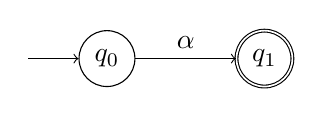
\begin{tikzpicture}
        \node[draw, circle] (A) at (0,0) {$q_0$};
        \draw[->] (-1,0) -- (A);
        \node[draw,circle,double] (B) at (2,0) {$q_1$};
        \draw[->] (A) -- (B);
        \draw (1,0) node [above] {$\alpha$};
     \end{tikzpicture}
     \rule{17cm}{0.5pt}\\
     \vspace{0.5cm}
     \caption{Automate reconnaissant $\alpha$ uniquement.}
     \label{fig:automate2}
 \end{figure}

 Nous allons maintenant prouver le sens réciproque. Pour cela, nous allons introduire une nouvelle classe d'automates, que l'on va appeler automates généralisés, dont les transitions seront étiquetées par des expressions rationnelles.

 \begin{defi}[Automate généralisé]
     Un automate généralisé est un automate dont la fonction de transition est définie par $\delta : \mathrm{Rat}(\Sigma)\times Q \to Q$ et qui ne possède qu'un état final. Un mot $u$ est accepté s'il peut être décomposé en $u_0\cdot u_1\cdots u_p$ et qu'il existe une suite $q_0,\ldots,q_{p+1}$ avec $q_{p+1}$ final et pour tout $i\leq p$, il existe $e\in\mathrm{Rat}(\Sigma)$ telle que $\delta(e,q_i)=q_{i+1}$ et $u_i\in L(e)$. De plus, on impose que $\delta$ n'est pas définie depuis $q_f$ l'état final et que $q_0$ n'est pas dans l'image de $\delta$.
 \end{defi}

 \begin{exo}
     Montrer que ces automates ont la même expressivité que les autres automates finis.
 \end{exo}

 \begin{rmk}
     Grâce à cet exercice, on peut supposer que pour tout automate $\aA$ il existe un automate généralisé $\aA'$ qui reconnaît le même langage.
 \end{rmk}

On va maintenant procéder sur l'automate généralisé en supprimant des transitions et des états jusqu'à n'obtenir qu'une seule transition, dont le label sera l'expression rationnelle associée à l'automate.

\begin{lem}[Réduction des transitions]
    Soit $\aA$ un automate généralisé, alors s'il existe $e,e'$ deux expressions et un état $q$ tels que $\delta(e,q)=\delta(e',q)$ alors on a un automate équivalent en supprimant ces deux transitions et en ajoutant $\delta(e+e',q)$.
\end{lem}

\begin{proof}
    Un mot reconnu par $\aA$ dont le chemin de lecture utilise $\delta(e,q)$ utilisera de la même façon $\delta(e+e',q)$, et réciproquement si un chemin de lecture utilise $\delta(e+e',q)$ alors soit le mot $u$ associé à cette transition est dans $L(e)$, auquel cas $\delta(e,q)$ donnera un chemin de lecture valide, soit il est dans $L(e')$ et $\delta(e',q)$ sera utilisé.
\end{proof}

On peut représenter cette réduction de la façon suivante :

\begin{figure}[htb]
    \centering
    \rule{17cm}{0.5pt}\\
    \vspace{0.5cm}
    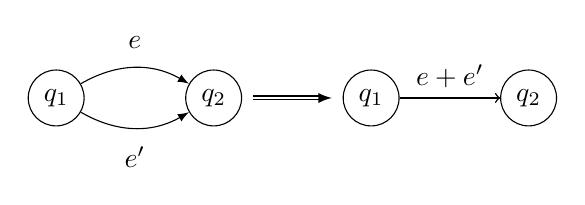
\begin{tikzpicture}
        \node[draw,circle] (A) at (-3,0) {$q_1$};
        \node[draw,circle] (B) at (-1,0) {$q_2$};
        \draw[->,>= latex] (A) to[bend left] (B);
        \draw[->,>= latex] (A) to [bend right] (B);
        \draw (-2,0.5) node [above] {$e$};
        \draw (-2,-0.5) node [below] {$e'$};
        \draw[->,>= latex, double distance = 1pt] (-0.5,0) -- (0.5,0);
        \node[draw,circle] (C) at (1,0) {$q_1$};
        \node[draw,circle] (D) at (3,0) {$q_2$};
        \draw[->,above] (C) -- (D);
        \draw[->,below] (C) -- (D);
        \draw (2,0) node [above] {$e+e'$};
    \end{tikzpicture}
    \rule{17cm}{0.5pt}\\
    \vspace{0.5cm}
    \caption{Réduction des transitions}
\end{figure}

Ainsi, par application successive du lemme, on peut supposer que l'on travail avec des états ne possédant qu'une transition entre deux états donnés. Nous allons maintenant procéder par élimination d'états.

\begin{lem}[\'Elimination des états]
    Soit un automate généralisé $\aA$ où l'on a réduit ses transitions, et $q$ un état ni initial ni final. Alors on peut construire un automate $\aA'$ reconnaissant le même langage en supprimant $q$ et, pour chaque couple d'états $(q_1,q_2)$ tel que $\delta(e_1,q_1)=q$ et $\delta(e_2,q)=q_2$, rajouter une transition de $q_1$ vers $q_2$ de la façon suivante :
    \begin{itemize}[label=$\bullet$]
        \item s'il existe $e$ telle que $\delta(e,q)=q$ alors on définit $\delta(e_1\cdot e^* \cdot e_2,q_1)=q_2$
        \item sinon, on définit $\delta(e_1\cdot e_2,q_1)=q_2$
    \end{itemize}
\end{lem}

\begin{proof}
    Dans le cas où le chemin de lecture ne passe pas par $q$, le lemme est évident. Supposons que dans la suite d'états $q_0,\ldots,q_p$ lisant un mot $u$ dans $\aA$ se trouve $q$, alors soit $q_1$ le prédécesseur de $q$ et $q_2$ son successeur (supposons d'abord que $q_2 \neq q$), dans la suite d'états. On sait qu'il existe une expression $e_1$ et une expression $e_2$ telles que $\delta(e_1,q_1)=q$ et $\delta(e_2,q)=q_2$ avec $u_1,u_2$ des parties du mot $u$ tels que $u_i\in L(e_i)$. Par définition, $u_1\cdot u_2\in L(e_1\cdot e_2)$ donc la suite d'états sans $q$ est valide dans $\aA$. Si jamais $q_2=q$, alors on peut remplacer toutes les suites de $q$ contiguës en disant que la transition est étiquetée par $e^*$ avec $e$ l'expression étiquetant la transition de $q$ à $q$.

    La réciproque est laissée en exercice au lecteur.
\end{proof}

On peut voit l'élimination d'états de la façon suivante :

\begin{figure}[htb]
    \centering
    \rule{17cm}{0.5pt}\\
    \vspace{0.5cm}
    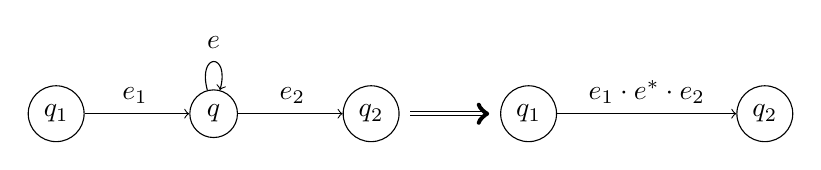
\begin{tikzpicture}
        \node[draw,circle] (A) at (-3,0) {$q$};
        \node[draw,circle] (B) at (-1,0) {$q_2$};
        \node[draw,circle] (E) at (-5,0) {$q_1$};
        \draw[->] (A) -- (B);
        \draw[->] (E) -- (A);
        \draw[->] (A) to[loop above] (A) ;
        \draw (-4,0) node [above] {$e_1$};
        \draw (-3,0.7) node [above] {$e$};
        \draw (-2,0) node [above] {$e_2$};
        \draw[->, double distance = 1pt] (-0.5,0) -- (0.5,0);
        \node[draw,circle] (C) at (1,0) {$q_1$};
        \node[draw,circle] (D) at (4,0) {$q_2$};
        \draw[->] (C) -- (D);
        \draw (2.5,0) node [above] {$e_1\cdot e^*\cdot e_2$};
    \end{tikzpicture}
    \rule{17cm}{0.5pt}\\
    \vspace{0.5cm}
    \caption{\'Elimination des états}
\end{figure}

On en déduit le résultat suivant :

\begin{prop}\label{prop:kleene2}
    Pour un automate généralisé $\aA$ il existe un automate généralisé $\aA'$ lisant le même langage et n'ayant qu'un état initial et un état final, et une seule transition entre les deux : le langage lu par $\aA'$ est exactement $L(e)$ pour $e$ l'étiquette de sa seule transition.
\end{prop}

\begin{proof}
    Il suffit de raisonner par récurrence sur le nombre d'états en appliquant l'élimination des états, et en réduisant les transitions qui en découlent. La dernière partie est par définition de la reconnaissance d'un mot dans un automate généralisé.
\end{proof}

On en déduit le théorème de Kleene :

\begin{them}[Kleene]
    La classe des langages rationnels est exactement l'ensemble des langages reconnus par des automates finis.
\end{them}

\begin{proof}
    C'est une conséquence directe des propositions \ref{prop:kleene1} et \ref{prop:kleene2}.
\end{proof}

\subsection{Myhill-Nérode}

Cette sous-section va s'attarder à une autre caractérisation des langages rationnels. Celle-ci est plus théorique mais présente plus facilement les limites des langages rationnels, et permet de répondre directement à la question \og y a-t-il pour un langage donné, un plus petit automate acceptant ce langage ?\fg{}

Tout d'abord, présentons un lemme en général utilisé pour montrer que des langages ne sont pas rationnels :

\begin{lem}[De l'étoile]
    Soit un langage rationnel $L$, alors il existe un nombre $M$ tel que pour tout mot $u\in L$ de longueur supérieure à $M$, il existe $v,w,x$ des mots ($w\neq\varepsilon$ mais les deux autres peuvent être vides) tels que $u = v\cdot w\cdot x$ et pour tout $n\in \nat$, $v\cdot w^n\cdot x \in L$. L'idée derrière est que pour les mots assez grands, il existe une partie du mot qui peut être répétée en restant dans le langage.
\end{lem}

\begin{proof}
    L'argument est principalement combinatoire : supposons que $u\in L$ avec $|u| > |Q|$ pour $Q$ l'ensemble d'états d'un automate $\aA$ reconnaissant $L$, alors lors de la lecture de $u$, on a la suite $q_0,\ldots,q_{|u|-1}$ et par principe des tiroirs, on trouve $i< j < |u|$ tels que $q_i = q_j$. On décompose alors le mot $u$ avec la partie préfixe $v := u_{<i}$, la partie infixe $w := u_{i,\ldots,j-1}$ et la partie postfixe $x := u_{j,\ldots,|u|-1}$. Dans ce cas, la lecture du mot $v\cdot w^n\cdot x$ donnera une suite d'états $q_0,\ldots,q_i$ puis $n$ fois la suite d'états de $q_i$ à lui-même décrite par $w$, puis la suite d'états $q_j,\ldots,q_{|u|-1}$  qui est un état final par hypothèse.
\end{proof}

\begin{rmk}
    Ce lemme est utile pour un langage infini : pour un langage fini, la constante sera simplement supérieure au cardinal du langage. De plus, la constante $M$ de ce lemme semble dépendre de l'automate reconnaissant le langage $L$, ce qui n'est pas naturel : le théorème de cette sous-section nous donnera justement une constante $M$ optimale et dépendant directement de $L$.
\end{rmk}

\begin{exo}
    En utilisant le lemme de l'étoile, montrer que le langage $\{0^n1^n\mid n\in\nat\}$ n'est pas rationnel.
\end{exo}

La notion principale pour pouvoir analyser les langages rationnels est celle de séparation des mots. L'idée derrière est simple : prenons deux mots $u$ et $v$, on peut les étendre naturellement en leur ajoutant un mot $z$ par concaténation, donnant $u\cdot z$ et $v\cdot z$. Dans ce cas, peut-on avoir un mot $z$ qui mène, depuis $u$, à un mot de $L$, et depuis $v$ à un mot qui n'est pas dans $L$ ? Cette notion motive notre prochaine définition :

\begin{defi}[Résiduel d'un langage]
    Soit $x$ un mot, on dénote par $x^{-1}L$ l'ensemble $$x^{-1}L=\{u\in \Sigma^*\mid x\cdot u \in L\}$$ appelé le résiduel de $L$ par $x$.

    De façon équivalente, on peut définir la relation d'équivalence d'inséparabilité : $x\sim y$ lorsque pour tout mot $u\in \Sigma^*$, $x\cdot u \in L \iff y\cdot u \in L$. Les classes d'équivalence pour cette relation sont les résiduels.
\end{defi}

Plusieurs observations s'ensuivent :
\begin{itemize}[label=$\bullet$]
    \item $L=\varepsilon^{-1}L$
    \item pour tout automate sur un langage $L$ fixé on peut associer à chaque état $q$ un résiduel de $L$.
\end{itemize}

Ces observations permettent d'imaginer les résiduels de $L$ comme un automate, lorsque le nombre de ses résiduels est fini. Le théorème de Myhill-Nérode stipule justement que ce nombre de résiduels est fini si et seulement si $L$ est rationnel.

\begin{them}[Myhill-Nérode]
    Soit $L$ un langage, alors $L$ est rationnel si et seulement s'il n'existe qu'un nombre fini de résiduels de $L$.
\end{them}

\begin{proof}
    Avec les observations antérieures, en supposant qu'il n'existe qu'un nombre fini de résiduels, on construit l'automate $\aA$ suivant :
    \begin{itemize}[label=$\bullet$]
        \item $Q = \{x^{-1}L\mid x \in \Sigma^*\}$
        \item $q_0 = \varepsilon^{-1}L$
        \item $\delta(\alpha,x^{-1}L) = (x\cdot \alpha)^{-1}L$ (la fonction est bien définie car si $x\sim y$ alors $x\cdot\alpha \sim y\dot\alpha$)
        \item $x^{-1}L$ est final s'il contient $\varepsilon$.
    \end{itemize}

    Si $x\in L$, alors $x^{-1}L$ contient $\varepsilon$ par construction, et s'il existe une suite d'états $q_0,\ldots,q_p$ menant à un état final dans cet automate, alors le dernier état est de la forme $x^{-1}L$ pour $x$ le mot lu et $\varepsilon\in x^{-1}L$ donc $x\cdot\varepsilon\in L$, c'est-à-dire $x\in L$. $L$ est donc reconnu par cet automate.

    Supposons que $L$ est rationnel. Alors soit $\aA$ un automate reconnaissant $L$. Pour chaque état $q$, on peut définir l'ensemble des mots menant de $q_0$ à $q$ : notons-le $P_q$. Alors pour deux mots $u,v\in P_q$, si $u\cdot z \in L$ alors $v\cdot z \in L$ car la lecture en partant de $q$ et en lisant les lettres de $z$ mène à un état final. Donc pour chaque état $q$, $P_q\subseteq x^{-1}L$ pour un certain $x$ (dépendant de $q$). On en déduit qu'il y a plus d'états que de résiduels, et comme l'automate est fini, qu'il y a un nombre fini de résiduels.
\end{proof}

\begin{rmk}
    La construction avec les résiduels nous donne donc aussi un automate minimal au sens du cardinal pour reconnaître un langage donné. Ainsi le lemme de l'étoile peut se reformuler en remplaçant \og il existe $M$\fg{} en remplaçant directement $M$ par le nombre de résiduels de $L$.
\end{rmk}

\begin{exo}
    Redémontrer que le langage $\{0^n1^n\mid n\in\nat\}$ n'est pas rationnel, cette fois-ci en utilisant le théorème de Myhill-Nérode.
\end{exo}

\begin{exo}
    L'ensemble des langages rationnels est-il stable par complémentaire ? Par intersection ?
\end{exo}

\begin{exo}
    Le langage des codes binaires de nombres multiples de $6$ est-il rationnel ?
\end{exo}

\begin{exo}
    Si $L$ est un langage rationnel, est-ce que le langage $\overline L$ des mots de $L$ à l'envers est rationnel ? Le langage des palindromes (mots qui sont les mêmes à l'envers) est-il rationnel ?
\end{exo}

La théorie des automates finis est bien plus vaste que le survol proposé ici : on peut par exemple parler de l'extension de ces automates aux mots infinis avec les automates de Büchi, ou encore de la détermination de l'arithmétique de Presburger avec des automates (ce dernier sujet aurait tout à fait sa place dans cet ouvrage dédié à la logique, mais comme l'objectif de ce chapitre n'est pas de voir en détail les automates mais seulement de mener naturellement aux machines de Turing, nous en ferons l'impasse).

Cependant, le problème avec les automates reste toujours le même : leur absence de mémoire et leur traitement purement linéaire de l'information. Le contre-exemple classique nous le montre bien : on ne peut pas compter de façon arbitrairement grande une valeur.


\subsection{Automates à pile}

Pour palier l'absence de mémoire de nos automates finis, l'idée naturelle est d'ajouter de la mémoire (jusque là, la solution paraît évidente). Il existe de nombreuses structures de données permettant de jouer la mémoire, mais comme l'indique le nom de nos automates, nous allons stocker les informations dans une pile, c'est-à-dire une structure linéaire de type \textit{last in first out}, où l'information extraite est la dernière information qui a été mise dans la pile. Le formalisme que nous utiliserons pour la pile est directement celui des mots : on peut représenter une pile par un mot $u$ sur lequel on ajoute ou enlève une lettre à gauche.

\begin{defi}[Automate à pile]
    Un automate à pile $\aA$ (non déterministe) est la donnée d'un tuple $(\Sigma,\Gamma,Q,q_0,\delta,F,\bot)$ où :
    \begin{itemize}[label=$\bullet$]
        \item $\Sigma$ est l'alphabet de lecture : c'est des mots de $\Sigma$ que l'on va reconnaître.
        \item $\Gamma$ est l'alphabet de pile : c'est avec cet alphabet que l'on écrira le mot qui nous servira de mémoire.
        \item $Q$ est l'ensemble des états.
        \item $q_0\in Q$ est toujours l'état initial.
        \item la fonction de transition est désormais $\delta : \Sigma^+\times \Gamma\times Q \to \mathcal P(\Gamma^*\times Q)$ où $A^+ = A \cup \{\varepsilon\}$
        \item $F\subseteq Q$ est l'ensemble des états finaux.
        \item $\bot\in \Gamma$ est le symbole de fond de pile : il indique que la pile est vide lorsqu'il est lu.
    \end{itemize}

    On appelle configuration interne une paire $(q,\gamma)\in Q \times \Gamma^*$ : cela représente l'état de l'automate à un instant donné. Une configuration est définie comme un triplet $(q,\gamma,u)\in Q\times \Gamma^*\times \Sigma^*$. On appelle transition entre deux configurations $(q,\alpha\cdot\gamma,\beta\cdot u)$ et $(q',\gamma'\cdot\gamma,u)$ la relation $(\gamma',q')\in\delta(\beta,\alpha,q)$, et on la note $(q,\alpha\cdot\gamma,\beta\cdot u) \vdash (q',\gamma'\cdot\gamma,u)$.

    On dit que le mot $u$ est accepté par $\aA$ s'il existe une suite de transitions depuis la configuration $(q_0,\bot,u)$ vers une configuration de la forme $(q_f,\gamma,\varepsilon)$ avec $q_f\in F$.
\end{defi}

Cette définition d'automate permet de définir la classe des langages algébriques, qui est une classe strictement plus large que les langages rationnels (elle contient par exemple le langage $\{0^n1^n\mid n\in\nat\}$)

Ceux-ci possèdent des propriétés de clôture différentes : ils sont clos par union, concaténation, et passage à l'étoile, mais aussi par passage au miroir. Enfin, l'intersection d'un langage rationnel et d'un langage algébrique est un langage algébrique.

Il existe une théorie parallèle, celle des grammaires, qui permet de donner une autre description équivalente des langages algébriques, mais nous ne nous attarderons pas dessus, car l'exemple des automates à pile nous sert surtout à introduire la notion de mémoire et de configuration. Remarquons simplement que la pile est un format de mémoire très limité : on peut y stocker des informations mais n'accéder qu'à une information à la fois. Nous allons donc voir un système plus expressif, avec une mémoire plus manipulable : les machines de Turing.

\section{Les machines de Turing}

L'idée des machines de Turing est assez similaire à celle d'automate à pile : simplement, au lieu d'utiliser une pile, nous utiliserons un ruban de mémoire, qui est une succession infinie de case, chacune contenant une lettre. La machine, au lieu de simplement prendre la lettre en haut de la pile, peut se déplacer librement sur le ruban pour lire et écrire sur le ruban de mémoire. Cette section sera dédiée à la présentation des machines de Turing, mais comportera peu de preuves : celles-ci, à cause du formmalisme lourd d'un système si complexe, sont trop techniques pour être présentées dans ce cours. Certaines idées de preuves seront données, tout de même.

\subsection{Des définitions équivalentes}

\begin{defi}[Machine de Turing]
    Une machine de Turing sur un alphabet $\Sigma$ est un tuple $(Q,\Gamma,q_0,\delta,q_a,q_r)$ où :
    \begin{itemize}[label=$\bullet$]
        \item $Q$ est l'ensemble des états de la machine.
        \item $\Gamma$ est l'alphabet de travail : c'est l'alphabet dans lequel seront les lettres du ruban de travail. On impose que $\Sigma\subseteq \Gamma$ et que $B\in\Gamma$ où $B$ est un symbole particulier, appelé symbole blanc, représentant l'absence d'écriture sur une case. On ajoute aussi le symbole $\rhd$ qui sera en début de ruban pour marquer qu'on est au début.
        \item $q_0$ est l'état initial de la machine.
        \item $\delta : Q\times \Gamma\to Q\times \Gamma \times \{\leftarrow,\rightarrow\}$ est la fonction de transition : elle considère l'état de la machine, la lettre lue et réécrit sur la case une nouvelle lettre, change d'état et fait bouger la tête de lecture vers la gauche ou la droite d'une case.
        \item $q_a\in Q$ est l'état acceptant : si la machine arrive dans cet état, le calcul s'arrête et le mot est accepté.
        \item $q_r\in Q$ est l'état de rejet : si la machine arrive dans cet état, le calcul s'arrête et le mot est rejeté.
    \end{itemize}
\end{defi}

Ces définitions ont peu de sens si l'on ne donne pas la définition de configuration et de ruban :

\begin{defi}[Ruban, configuration, transition]
    Le ruban de travail est un mot infini $r\in \Gamma^\omega$ sur l'alphabet de travail. On appelle configuration un tuple $(q,i,r)$ où $q$ est l'état de la machine de Turing, $r$ est le ruban et $i$ est l'indice de la case sur laquelle se trouve la tête de lecture. Plutôt que de noter cela comme un tuple, on note en général une configuration par un mot de la forme $r_{<i}qr_{\geq i}$, c'est-à-dire que l'on écrit les symboles qui sont à gauche de la tête de lecture, puis l'état dans lequel est la machine, puis le reste du mot. La tête de lecture se trouve donc sur la lettre juste à droite de l'état $q$ dans cette représentation.

    On appelle transition la fonction entre configurations définie de façon naturelle par la fonction de transition, en partant de la configuration $u\alpha q\beta r$ :
    \begin{itemize}
        \item si $\delta(q,\beta) = (q',a,\leftarrow)$ alors la transition sera $u\alpha q\beta r \to uq'\alpha a r$
        \item si $\delta(q,\beta) = (q',a,\rightarrow)$ alors la transition sera $u\alpha q\beta r \to u\alpha a q r$
    \end{itemize}

    On appelle calcul la suite de transitions depuis une configuration donnée (comme la machine est déterministe, la suite est unique, potentiellement infinie).
\end{defi}

De plus, on note $B^\infty$ la fin du ruban (remplie forcément de $B$ à l'infini).

\begin{defi}[Acceptation, rejet]
    Soit $x$ un mot sur un alphabet $\Sigma$ et $\MM$ une machine de Turing sur $\Sigma$. On dit que $\MM$ accepte $x$ si le calcul sur la configuration $q_0\rhd x B^\infty$ finit par $\MM$ entrant dans l'état $q_a$. On dit que $\MM$ rejette $x$ si le calcul sur la même configuration finit par $\MM$ entrant dans l'état $q_r$.
\end{defi}

\begin{rmk}
    Un mot $x$ peut n'être ni accepté, ni rejeté.
\end{rmk}

Donnons un exemple imagé d'une machine $\MM$ agissant sur la configuration $\rhd 0q1B^\infty$ en supposant que $\delta(q,1)=(0,q',\leftarrow)$ :

\begin{figure}[htb]
    \centering
    \rule{17cm}{0.5pt}\\
    \vspace{0.5cm}
    \begin{tikzpicture}
        \draw (-5,1) -- (5,1) -- (5,-1) -- (-5,-1) -- (-5,1);
        \draw (-3,1) -- (-3,-1);
        \draw (-1,1) -- (-1,-1);
        \draw (1,1) -- (1,-1);
        \draw (3,1) -- (3,-1);
        \draw[dashed] (5,1) -- (5.5,1);
        \draw[dashed] (5,-1) -- (5.5,-1);
        \draw (-4,0) node {\Huge $\rhd$};
        \draw (-2,0) node {\Huge $0$};
        \draw (0,0) node {\Huge $1$};
        \draw (2,0) node {\Huge $B$};
        \draw (4,0) node {\Huge $B$};
        \draw[<-] (0,-1) -- (0,-2);
        \draw (0,-1.5) node [right] {\Large $q$};

        \draw (-2,-2) -- (2,-2) -- (2,-4) -- (-2,-4) -- (-2,-2);
        \draw (0,-3) node {\Huge $\MM$};
        \draw[<-] (-2,-5) -- (-2,-4.5) -- (0,-4.5) -- (0,-4);
        \draw (0,-4.5) node [right] {\Large $q'$};
        
        \draw (-5,-5) -- (5,-5) -- (5,-7) -- (-5,-7) -- (-5,-5);
        \draw (-3,-5) -- (-3,-7);
        \draw (-1,-5) -- (-1,-7);
        \draw (1,-5) -- (1,-7);
        \draw (3,-5) -- (3,-7);
        \draw[dashed] (5,-5) -- (5.5,-5);
        \draw[dashed] (5,-7) -- (5.5,-7);
        \draw (-4,-6) node {\Huge $\rhd$};
        \draw (-2,-6) node {\Huge $0$};
        \draw (0,-6) node {\Huge $0$};
        \draw (2,-6) node {\Huge $B$};
        \draw (4,-6) node {\Huge $B$};
    \end{tikzpicture}
    \rule{17cm}{0.5pt}\\
    \vspace{0.5cm}
    \caption{Illustration de l'exécution d'une machine de Turing}
\end{figure}

Plusieurs versions équivalentes des machines de Turing existent, nous allons donner une liste et une façon de les simuler avec une machine à un ruban telle que décrite ici :
\begin{itemize}[label=$\bullet$]
    \item La machine peut se retrouver sur un ruban infini des deux côtés. Dans ce cas, comme on a une bijection entre $\nat$ et $\mathbb Z$ qui envoie $-n$ sur $2n+1$ et $n$ sur $2n$, il nous suffit de créer des états qui permettent de gérer des transitions de deux cases à chaque fois qu'il faut faire une transition d'une case, sauf sur la case d'indice $0$ où un changement d'état indiquera comment se comporter.
    \item On peut changer l'alphabet, et coder par exemple n'importe quel alphabet fini $\Sigma$ avec $\{0,1\}$ en considérant les cases par paquets (suffisamment gros pour pouvoir coder chaque élément de $\Sigma$ par un nombre binaire), ce qui augmentera largement le nombre d'états mais fonctionne. C'est d'ailleurs ce qu'il se passe dans les ordinateurs, où l'on code les données par paquets de $32$ ou $64$ bits.
    \item On peut considérer plusieurs rubans, et chaque tête de lecture se déplacera indépendamment. On peut simuler cela sur un ruban en considérant un alphabet plus gros : chaque case consistera en le $n$-uplet de cases de la machine à plusieurs rubans. Il faut néanmoins gérer le fait de bouger dans des sens différents : on peut pour cela considérer un alphabet encore plus gros qui serait constitué de parties de l'ancien alphabet et permettrait de faire une machine non déterministe.
    \item Une machine non déterministe peut se simuler avec une machine déterministe : chaque fois que plusieurs transitions sont possibles, on effectue une transition, puis on \og backtrack\fg{} (fait la transition inverse) pour faire l'autre transition. On effectue cette démarche pour chaque suite de transitions possibles de longueur $k$ et par $k$ croissant.
\end{itemize}

En bref, notre modèle est très expressif, mais malheureusement très peu manipulable dans le sens où se donner une machine de Turing concrète est très fastidieux. Nous n'en donnerons d'ailleurs pas ici : nous n'en donnerons que des codes, c'est-à-dire des suites de symboles qui peuvent être traduites en une machine de Turing. Plus précisément, tout algorithme écrit en pseudo-code correspondra à une machine de Turing (on l'admet ici).

Enfin, on peut construire une version équivalente des machine de Turing où, au lieu d'avoir des états acceptant et rejetant, on a un simple état d'arrêt, et la machine retourne le mot écrit sur le ruban lorsqu'elle s'arrête (puisque le mot infini contient une infinité de $B$, il le mot retourné est bien un mot fini). On appelle ces fonctions $\Sigma^*\to \Sigma^*$ des fonctions partielles calculables. On dit qu'une fonction est calculable quand elle est totale calculable.

\subsection{Les principaux théorèmes}

Un premier théorème fondamental dans la théorie de la calculabilité est celui qu'il existe une machine universelle :

\begin{them}
    Il existe une machine de Turing dite universelle, $\mathcal U$ sur un alphabet $\Sigma$ telle que, pour toute machine de Turing $\MM$ codée dans $\Sigma$ (le codage $\encode{\;}$ dépend de $\mathcal U$) et toute entrée $x$ codée dans $\Sigma$, $\mathcal U$ accepte $\langle \encode M,x\rangle$ si et seulement si $M$ accepte $x$, et refuse $\langle \encode M,x\rangle$ si et seulement si $M$ refuse $x$.
\end{them}

Comme dit plus tôt, nous ne donnerons pas de preuves pour ce genre de théorèmes, nous nous convaincrons seulement que l'on arrive en effet à coder un interpréteur pour un langage informatique donné, ce qui est l'analogue informatique d'une machine de Turing universelle.

La notation $\langle x,y\rangle$ sert à parler du codage d'un couple. Un codage simple dans l'alphabet $\{0,1\}$ est $1^{|x|}0 x y$ : l'information nous est donnée en comptant le nombre de $1$ de quelle taille fait $x$.

Le théorème suivant dit qu'on peut exécuter une machine sur elle-même :

\begin{them}[Récursion de Kleene]
    Soit $t$ une fonction calculable, il existe alors une machine de Turing $F$ telle que $t\encode F$ est une machine équivalente à $F$.

    Une version équivalente est qu'une machine $\MM$ a accès à son code source $\encode\MM$.
\end{them}

\subsection{Langage récursif, récursivement énumérable}

Naturellement, nous pouvons associer à une machine $\MM$ le langage $L(\MM)$ des mots reconnus par $\MM$. Cependant, on peut remarquer une différence importante : là où dans les anciens automates la lecture était linéaire et donc terminait forcément, ici nous n'avons aucune garantie que l'exécution d'une entrée $x$ sur $\MM$ va arriver à un état acceptant ou refusant. Ceci signifie qu'il existe deux classes de langages bien différentes :
\begin{itemize}[label=$\bullet$]
    \item les langages dits décidables, ou récursifs, qui sont ceux de la forme $L(\MM)$ pour une machine de Turing donnée qui, sur toute entrée, termine (i.e. tout calcul sur une entrée $x$ mène à un des deux états $q_a$ ou $q_r$).
    \item les langages dits récursivement énumérables, qui sont ceux de la forme $L(\MM)$ pour une machine de Turing $\MM$ (qui peut donc ne pas terminer).
\end{itemize}

De même, on différencie comme on l'a dit plus tôt les fonctions calculables des fonctions calculables partielles. Pour montrer l'importance de cette distinction, nous allons montrer qu'il existe des langages récursivement énumérables non récursifs.

\begin{rmk}
    Le nom de \og récursivement énumérable\fg{} vient du fait qu'une condition équivalente est qu'il existe une machine $\MM$ donnant la liste de tous les éléments du langage : une machine qui les énumère, donc. (\'Evidemment, ça ne suffit pas à décider si une entrée $x$ est dans le langage, puisqu'il faudrait avoir accèd à l'entièreté de la liste, en général infinie.)
\end{rmk}

\begin{defi}[Problème de l'arrêt]
    Soit $\mathrm{HALT} = \{\langle \encode \MM,x\rangle\mid \MM \text{ s'arrête sur l'entrée } x\}$. HALT est récursivement énumérable mais pas récursif.
\end{defi}

\begin{proof}
    L'existence d'une machine de Turing universelle suffit à montrer que le langage est récursivement énumérable : on exécute $\MM$ sur $x$ avec une machine universelle, et si elle termine on entre dans l'état acceptant. Maintenant, supposons que HALT soit récursif. On a donc une machine $\MM$ qui peut dit si une machine s'arrête sur une entrée donnée. On définit alors le programme $f$ suivant, prenant en entrée $x$ :
    \begin{itemize}[label=$\bullet$]
        \item si $\langle \encode x,x\rangle\in\mathrm{HALT}$ alors on crée une boucle infinie.
        \item sinon, on entre dans l'état $q_a$.
    \end{itemize}
    On remarque alors que, d'après le théorème de Kleene, on peut exécuter le programme $f$ en prenant son code en entrée : alors si $\langle \encode f,f\rangle \in\mathrm{HALT}$ on en déduit que $f(f)$ entre dans une boucle infinie, donc $\langle \encode f,f\rangle \notin\mathrm{HALT}$ et de même si $\langle \encode f,f\rangle\notin\mathrm{HALT}$ on en déduit que $\langle\encode f,f\rangle\in\mathrm{HALT}$.
\end{proof}

Un problème dont on sait qu'il n'est pas récursif est dit indécidable : c'est le cas du problème de l'arrêt, mais plus généralement d'une très large classe de langages. En effet, le prochain théorème montre que tout langage défini par une propriété non triviale (c'est-à-dire autre que toujours vraie ou toujours fausse) sur un langage récursivement énumérable est indécidable. On appelle une telle propriété une propriété sémantique : elle porte sur un langage récursivement énumérable, par contraste avec une propriété syntaxique qui porte sur les machines elles-mêmes (on peut par exemple compter le nombre de boucle \textit{While} d'un programme : les propriétés syntaxiques décrivent souvent des ensembles récursifs.

\begin{them}[Rice]
    Soit RE la classe des langages récursivement énumérables sur un alphabet $\Sigma$. Soit une partie $E$ de RE (donc une classe de langage), et $P$ l'ensemble des machines qui reconnaissent un ensemble $A\in E$ (donc les machines $\MM$ telles que $L(\MM)\in E$). $P$ est récursif si et seulement si $E=\varnothing$ ou $E=\mathrm{RE}$. 
\end{them}

\begin{exo}
    Montrer ce théorème en montrant que si $P$ est non trivial alors il peut se réduire au problème de l'arrêt, c'est-à-dire construire à partir d'un $P$ fixé une entrée du problème de l'arrêt, que l'on sait indécidable.
\end{exo}

\subsection{Fonctions récursives}

Le formalisme des machines de Turing permet d'avoir une approche qui fait un lien fort avec l'informatique, puisqu'il est le formalisme à la base même des ordinateurs et de la notion de programme et de code. Cependant, pour l'étude logique, un autre formalisme équivalent va être privilégié : celui des fonctions récursives. Nous allons donc voir les fonctions récursives, d'abord par les fonctions récursives primitives, et nous verrons ensuite l'équivalence entre fonction récursive et fonction calculable par une machine de Turing.

\subsubsection{Fonctions récursives primitives}

\begin{defi}[Classe RP]
On définit la classe des fonctions récursives primitives RP comme le plus petit sous-ensemble de fonctions $\nat^k\to\nat$, $k$ parcourant $\nat$, tel que :
\begin{itemize}[label=$\bullet$]
    \item pour chaque $n\in\nat$ et $k\in\nat$, la fonction $n : \nat^k\to\nat, x \mapsto n$ est dans RP.
    \item $S : \nat \to \nat, x \mapsto x+1$ est dans RP.
    \item les fonctions $\pi_i^k : \nat^k\to\nat, (x_1,\ldots,x_k)\mapsto x_i$ sont dans RP.
    \item si $f_1,\ldots,f_k : \nat^n \to \nat$ sont des fonctions de RP et $h : \nat^k\to\nat$, alors la fonction $h\langle f_1,\ldots,f_k\rangle : \nat^n \to\nat, x \mapsto h(f_1(x),\ldots,f_k(x))$ est aussi dans RP.
    \item si $f : \nat^k\to\nat$ et $g : \nat^{k+2}\to\nat$ sont des fonctions de RP, alors la fonction $\rec(f,g) : \nat^{k+1} \to\nat$ est dans RP, où \begin{align*}
        \rec(f,g)(x,0) &= f(x)\\
        \rec(f,g)(x,S(n)) &= g(x,n,\rec(f,g)(x,n))
    \end{align*}
\end{itemize}
\end{defi}

Le point important pour l'expressivité de cette classe de fonction est évidemment le fait d'autoriser les appels récursifs. On peut construire de nombreuses fonctions usuelles par cette classe.

\begin{exo}
    Montrer que les fonctions suivantes sont dans RP :
    \begin{itemize}[label=$\bullet$]
        \item La fonction identité $x \mapsto x$
        \item La fonction somme : $\nat^2\to\nat, (x,y)\mapsto x+y$
        \item La fonction produit : $\nat^2\to\nat, (x,y)\mapsto x\times y$
        \item La fonction puissance : $\nat^2\to\nat, (x,y)\mapsto x^y$
        \item La fonction prédécesseur : $\nat\to\nat, x \mapsto \max(0,x-1)$
        \item La fonction différence : $\nat^2\to\nat, (x,y)\mapsto \max(0,x-y)$
        \item La fonction moitié : $\nat\to\nat,x \mapsto \lfloor x/2\rfloor$
        \item La fonction division : $\nat^2\to\nat, (x,y)\mapsto \lfloor x/y\rfloor$ et $0$ si $y=0$
        \item La fonction reste : $\nat^2\to\nat, (x,y)\mapsto x\%y$ le reste de $x$ par la division par $y$, et $0$ si $y=0$
        \item Pour tout polynôme de $\nat[X]$, la fonction $\nat\to\nat$ associée.
        \item Pour $f,g,h$ trois fonctions de RP, la fonction $\texttt{if}(f,g,h) : x \mapsto g(x)$ si $f(x)=0$ et $h(x)$ sinon.
    \end{itemize}
\end{exo}

\begin{exo}\label{exo:bij}
    Montrer que la fonction $b : \nat^2\to\nat, (x,y)\mapsto \frac{1}{2}(x+y)(1+x+y)+y$ établit une bijection entre $\nat^2$ et $\nat$. Construire aussi les fonction $\pi_1$ et $\pi_2$ telles que $\pi_1(b(x,y))=x$ et $\pi_2(b(x,y))=y$.
\end{exo}

On peut aussi analyser des ensembles grâce à leur fonction caractéristique.

\begin{exo}
    Construire les fonctions caractéristiques des ensembles suivants :
    \begin{itemize}[label=$\bullet$]
        \item $\nat_{>k}$ pour $k\in\nat$
        \item $\{0\}$
        \item $n\nat$
        \item $\{(x,x)\mid x\in\nat\}$
        \item $\{(x,y)\mid x < y\}$
        \item $\{(x,y)\mid y=P(x)\}$ où $P\in\nat[X]$ est fixé.
    \end{itemize}
\end{exo}

\subsubsection{Opérateur mu}

Cependant, toutes les fonctions calculables par des machines de Turing ne sont pas forcément dans RP : certaines croissent trop vite. En effet, une remarque assez directe est que les fonctions récursives primitives ne peuvent pas appliquer une fonction un nombre non borné de fois : il faut calculer au préalable une borne supérieure du nombre d'application de notre fonction. De plus, toutes les fonctions dans RP sont des fonctions totales, alors que nous voulons pouvoir écrire des fonctions partielles. Nous allons donc définir Rec, la classe des fonctions récursives, en ajoutant un constructeur :

\begin{defi}[Classe Rec]
    La classe Rec est la classe RP à laquelle on ajoute le constructeur $\mu$ : si $f : \nat^{k+1}\to\nat$ est dans Rec, alors $g(x_1,\ldots,x_k)=\mu(y,f)$ renvoie le plus petit $y$ tel que $f(x_1,\ldots,x_k,y) = 0$ et pour tout $x<y$, $f(x_1,\ldots,x_k,x)$ est définie, et n'est pas définie sinon.
\end{defi}

Il se trouve que Rec est exactement la classe des fonctions calculables partielles.

\begin{them}[Simulation des machines de Turing]
    Soit $\MM$ une machine de Turing sur $\{0,1\}$ définissant une fonction $f : \nat \to \nat$ à partir de son comportement sur $\{0,1\}^*\to\{0,1\}^*$. Alors $f\in\mathrm{Rec}$.
\end{them}

\begin{proof}
    Nous allons pour cela construire par étape une fonction $f$ récursive qui simule $\MM$ :
    \begin{itemize}[label=$\bullet$]
        \item Nous allons coder les états de $\MM$ par des entiers.
        \item Une configuration peut être vue comme un élément de $\nat^3$ avec ce codage : nous allons donc construire une fonction qui effectue une transition, ou plus précisément trois fonctions, l'une retournant le nouvel indice de la tête de lecture, la deuxième retournant le code de l'état et la troisième retournant la forme nouvelle du ruban.
        \item Cette fonction peut se faire par disjonction de cas : on sait coder la fonction caractéristique de chaque entier, et faire des branchements if/then/else. Il ne reste qu'à effectuer cette disjonction de cas sur chaque état en entrée, puis une disjonction de cas suivant si le symbole lu est $0$ ou $1$. La fonction d'indice décrémente ou incrémente l'indice directement, ce que l'on peut faire, la fonction d'état associe une constante, et la fonction de ruban n'a qu'à effectuer de l'arithmétique pour ajouter ou soustraire $2^i$ avec $i$ l'indice de la tête de lecture.
        \item Si l'on nomme $g$ cette fonction, on peut alors l'appliquer en boucle jusqu'à obtenir un résultat. C'est ici que l'on a besoin de $\mu$, qui s'appliquera à la fonction caractéristique de l'état d'arrêt composée avec la fonction qui pour $i$ effectue $i$ itérations de $g$.
    \end{itemize}
\end{proof}

\begin{rmk}
    La construction d'une fonction récursive simulant une machine de Turing ne nécessite l'opérateur $\mu$ que pour pouvoir appliquer l'opération de transition un nombre non borné de fois : cela signifie que pour une machine $\MM$ où l'on peut borner son temps de calcul en fonction de son entrée, il suffit d'une fonction primitive récursive pour coder la machine $\MM$.
\end{rmk}


\chapter{Arithmétique de Peano et incomplétude}

Nous avons étudié la logique des prédicats, mais ne l'avons pas encore mise en \oe uvre. Ce chapitre en sera une première application : nous allons introduire l'axiomatisation de l'arithmétique de Peano, c'est-à-dire la théorie axiomatique définissant les entiers naturels usuellement. Nous commencerons donc par énoncer les axiomes de la théorie nommée PA, pour ensuite définir quelques propriétés basiques. Historiquement, l'axiomatisation de l'arithmétique a été la première réussite du logicisme : réussir à formuler de façon purement formelle ce que nous entendons par les entiers et leurs relations usuelles. C'est cette réussite qui a mené David Hilbert à poser la question à toute la communauté scientifique : \og arriverons-nous à décider toute proposition arithmétique de façon purement mécanique ?\fg{} (Nous dirions maintenant \og existe-t-il un algorithme décidant les proposition vraies ?\fg{} mais le problème a été posé avant que la théorie de la calculabilité émerge). La réponse, bien connue maintenant, est non : non seulement il n'existe pas d'algorithme permettant de décider les propositions, mais tout système suffisamment expressif pour parler de toute l'arithmétique, mais suffisamment restreint pour être manipulable, possède des propositions qui sont indécidables, c'est le premier théorème d'incomplétude de Gödel. Nous reviendrons à la fin du chapitre sur ce théorème, ainsi que le second, qui sont des passages obligés du traitement moderne de la logique. Bien sûr, nous avons maintenant l'outil de la calculabilité qui rendra beaucoup plus digeste (bien que toujours très dur à assimiler) la preuve que nous ferons du premier théorème, là où historiquement la preuve est plus vieille que la notion de machine de Turing. Le second théorème d'incomplétude sera mentionné mais non développé, pour des raisons que nous développerons dans la dernière section.

\section{Axiomes de Peano}

Nous allons donc expliciter la théorie axiomatique PA. Pour cela, donnons d'abord le langage de l'arithmétique : $\LL=\{0,S,+,\times\}$ où, sans surprise, $0$ est une constante, $S$ une fonction d'arité $1$ représentant la fonction $x\mapsto x+1$, $+$ et $\times$ des fonctions d'arité $2$. On pourrait ajouter $\leq$ une relation binaire, mais nous allons voir que nous pouvons la définir de façon peu coûteuse. L'idée de notre définition de $\nat$ est que $\nat$ est défini comme une structure inductive avec une constante et un constructeur unaire.

Plutôt que d'énoncer tous les axiomes de Peano à la suite, nous allons nous concentrer sur chacun d'eux (ou au moins chaque groupe). 

\begin{defi}[Axiomes du successeur]
    Le premier axiome est $A_1 := \forall x. \lnot (S x = 0)$, nous nous permettrons d'écrire $\lnot (a=b)$ par $a\neq b$.

    Le second axiome est $A_2 := \forall x. \exists y.(x\neq 0 \to S y = x)$.

    Le troisième axiome est $A_3 := \forall x.\forall y. ((S x = S y)\to (x=y))$
\end{defi}

Ces axiomes traduisent le comportement de l'opération $S$ : $0$ n'est le successeur de personne, mais tout autre élément est le successeur d'au moins un élément, et la fonction $S$ est injective (donc il n'existe finalement qu'un seul prédécesseur à un entier non nul). Les axiomes qui suivent définissent $+$ et $\times$ :

\begin{defi}[Axiomes de l'addition]
    Les deux axiomes suivants sont :
    \begin{align*}
        A_4 &:= \forall x. (x+0=x)\\
        A_5 &:= \forall x. \forall y. x + (S y) = S (x + y)
    \end{align*}
\end{defi}

Ces axiomes traduisent directement la définition récursive de l'addition. De même les deux axiomes suivants définissent la multiplication de façon récursive :

\begin{defi}[Axiomes de la multiplication]
    Les deux axiomes suivants sont :
    \begin{align*}
        A_6 &:= \forall x. (x\times 0 = 0)\\
        A_7 &:= \forall x.\forall y. x\times (S y) = (x\times y) + x
    \end{align*}
\end{defi}

On note alors $\PA_0$ la théorie $\PA_0 = \{A_1,A_2,A_3,A_4,A_5,A_6,A_7\}$. Cette théorie est très faible : elle ne permet aucune preuve par récurrence. Ceci est dû au fait qu'a priori, tous les éléments ne sont pas forcément des successeurs de $0$ : simplement qu'un élément est localement un successeur ou $0$. Cependant, si l'énoncé commun de la récurrence est \og toute partie $F\subseteq\nat$ contenant $0$ et stable pour $S$, càs telle que $x\in F \implies S x \in F$ alors $F=\nat$\fg{}, cette quantification sur les parties $F\subseteq\nat$ n'est pas définissable dans notre théorie du premier ordre (c'est exactement une quantification du second ordre). Cependant, de la façon dont on se sert de la récurrence, on remarque que la notion importante est celle de proposition, et non de sous-ensemble : on veut que toute proposition vraie pour $0$ et dont la vérité à un rang implique sa vérité au rang suivant est vraie pour tous les objets. Cette version peut se faire, pour une proposition donnée : il suffit d'écrire pour une proposition $P$ la proposition $P(0)\land (\forall x.P(x)\to P(S(x)))\to \forall x. P(x)$ et de l'ajouter en axiome. L'idée est donc, alors, d'ajouter autant d'axiomes que nous avons de propositions : on va définir alors ce qu'on appelle un schéma d'axiomes (c'est-à-dire un ensemble d'axiomes dont on décrit la forme, de façon équivalente dont on donne un algorithme de construction).

\begin{defi}[Schéma d'axiomes de récurrence]
    Pour $P$ une proposition à $n$ variables libres $x_0,\ldots,x_n$, la proposition $$\forall x_1.\ldots\forall x_n.((P(0,x_1,\ldots,x_n)\land \forall x.(P(x,x_1,\ldots,x_n)\to P(S(x),x_1,\ldots,x_n)))\to \forall x. P(x,x_1,\ldots x_n))$$ appartient à l'ensemble $\mathcal P_\mathrm i$.
\end{defi}

\begin{lem}[Récursivité de la récurrence]
    L'ensemble $\mathcal P_\mathrm i$ est un langage récursif (et donc décidable) sur $(\LL\cup\{(,),\lor,\land,\to,\lnot,\forall.,\exists.\})^*$.
\end{lem}

\begin{proof}
    Nous ne donnerons pas une réelle démonstration ici mais une idée de pourquoi le résultat est vraie (une démonstration rigoureuse nécessiterait d'entrer en détails dans le fonctionnement des machines de Turing, ce que nous nous refusons de faire pour garder une certaine lisibilité). Ce résultat vient directement du fait qu'on a donné une description algorithmique de $\mathcal P_\mathrm i$ (on pourrait penser que cela nous donne uniquement un ensemble récursivement énumérable, mais on peut par exemple ordonner les propositions par longueur et considérer le nombre de symboles de la proposition dont on veut savoir si elle est dans $\mathcal P_\mathrm i$ : il n'y aura qu'un nombre fini de propositions plus petites qu'il faudra donc tester).
\end{proof}

On peut alors définir PA comme l'ensemble précédent muni du schéma d'axiomes de récurrence.

\begin{defi}[Théorie PA]
    On définit $\PA := \PA_0 \cup \mathcal P_\mathrm i$.
\end{defi}

\begin{lem}[Récursivité de PA]
    PA est un langage récursif.
\end{lem}

\begin{proof}
    Il suffit de tester pour une proposition si elle est l'une des $7$ premières puis d'exécuter l'algorithme pour vérifier si la proposition est dans $\mathcal P_\mathrm i$.
\end{proof}

\begin{exo}
    Montrer que les axiomes de $\mathcal P_\mathrm i$ peuvent être remplacés par une nouvelle règle :
    \begin{center}
        \begin{prooftree}
            \hypo{\Gamma\vdash P(0)}
            \hypo{\Gamma\vdash \forall x. P(x)\to P(S(x))}
            \infer2[Rec]{\Gamma\vdash \forall x. P(x)}
        \end{prooftree}
    \end{center}
    et que l'on peut alors définir PA comme la théorie $\PA_0$ enrichie de cette règle logique dans la relation de dérivation de jugement logique. \textit{Remarque : Cette règle n'a de sens que dans le langage de l'arithmétique, et on présuppose largement que $\Gamma\subseteq\PA_0$ pour que la règle ait un sens.}
\end{exo}

\begin{exo}
    Montrer qu'il existe un modèle non standard de PA, c'est-à-dire un modèle qui n'est pas l'ensemble usuel des entiers naturels. \textit{Indication : on introduira une constante dont on montrera qu'elle n'est égale à aucun entier naturel en utilisant le théorème de compacité.}
\end{exo}

\section{L'arithmétique telle que nous la connaissons}

On peut alors commencer à prouver des résultats semblant évidents mais qui n'appartiennent pas directement à la théorie. Nous ne donnerons pas d'arbre de preuve mais seulement des arguments. Leur mise en arbre de preuve sera laissée en exercice.

\begin{prop}[Neutre]
    $0$ est neutre pour $+$, c'est-à-dire que \begin{align*}
        \forall x.x+0=x\\
        \forall x.0+x=x
    \end{align*}

    $1$ est neutre pour $\times$ :
    \begin{align*}
        \forall x. x\times 1=x\\
        \forall x. 1\times x=x
    \end{align*}
\end{prop}

\begin{proof}
    La première proposition est purement un axiome de notre théorie, mais la neutralité à gauche de $0$ est déjà à prouver (par récurrence évidemment). D'abord $0+0=0$ en appliquant l'axiome $A_4$, puis si $0+x=x$ alors $0+(S x) = S (0+x) = S x$ en remplaçant $0+x$ par $x$ grâce à l'hypothèse. Donc pour tout $x$, $0+x=x$.

    La neutralité à droite de $1$ pour $\times$ est un simple calcul :
    \begin{align*}
        x\times 1 &= x\times (S 0)\\
        &= (x\times 0) + x\\
        &= x
    \end{align*}
    pour la neutralité à gauche, nous allons encore raisonner par récurrence : d'abord $1\times 0 = 0$ grâce à l'axiome $A_6$, puis si l'on suppose que $1\times n = n$ alors $1\times (S n) = (1\times n) + 1$ puis on remarque que $n+1=S n$ de façon directe, eet que $1\times n = n$ par hypothèse de récurrence, nous donnant que $1\times (S n) = S n$.
\end{proof}

\begin{prop}[Associativité et commutativité de l'addition]
    L'addition est associative et commutative, ce qui signifie :
    \begin{align*}
        \forall x.\forall y.\forall z. x+(y+z) = (x+y)+z\\
        \forall x.\forall y. x+y = y+x
    \end{align*}
\end{prop}

\begin{proof}
    Prouvons le premier point par récurrence sur $z$ (quitte à échanger les variables) : dans le premier cas, on a $x+y=x+y$ après réduction des additions de $0$ à droite. Si l'on suppose que $x+(y+z)=(x+y)+z$ alors $x+(y+S z) = x+S(y+z)=S(x+(y+z))$ et ici, par hypothèse de récurrence, on peut remplacer $x+(y+z)$ par $(x+y)+z$ et on finit la chaîne d'égalités par $S((x+y)+z) = (x+y) + Sz$, prouvons la propriété par récurrence.

    Pour le deuxième point, nous prouverons un lemme intermédiaire : $\forall x.\forall y. S(x+y)=Sx+y$ par récurrence sur $y$ : dans le cas nul, on a $S(x+0) = S(x) + 0$ qui est vrai. Si $\forall x.S(x+y)=Sx+y$, alors $Sx+Sy = S(Sx+y)$ et par application de l'hypothèse de récurrence, en remplaçant $x$ par $Sx$, on en déduit que $S(Sx+y) = SS(x+y)$, et $SS(x+y) = S(x+Sy)$ donc $$Sx+Sy=S(x+Sy)$$ ce qui complète notre démonstration par récurrence.

    Montrons maintenant la commutativité par récurrence sur $y$ : dans le cas nul, on doit montrer que $x+0=0+x$ ce qui se fait grâce au fait que $0$ est neutre. Supposons que $\forall x. x+y=y+x$, alors en fixant un certain $x$, $x+Sy=S(x+y)$ puis par hypothèse de récurrence, $S(x+y)=S(y+x)$ et en utilisant le lemme précédent, $S(y+x)=Sy+x$, donc $$x+Sy=Sy+x$$ concluant notre preuve par récurrence.
\end{proof}

Nous allons maintenant prouver la distributivité.

\begin{prop}[Distributivité]
    La multiplication est distributive sur l'addition, c'est-à-dire que : $$\forall x.\forall y.\forall z.x\times(y+z) = x\times y + x\times z$$ en prenant les conventions de priorité habituelles, et $$\forall x.\forall y.\forall z. (x+y)\times z = x\times z + y\times z$$
\end{prop}

\begin{proof}
    Prouvons le premier résultat par récurrence sur $z$ : dans le cas où $z=0$, on trouve $\forall x.\forall y.x\times (y+0) = x\times y + x\times 0$, ce qui se vérifie facilement. Dans le cas où $\forall x.\forall y. x\times (y+z) = x\times y + x\times z$, alors pour $x,y$ fixéx, \begin{align*}    x\times (y+Sz)&=x\times S(y+z) \\
     &= (x\times (y+z)) + x \\
     &= (x\times y + x\times z) + x\\
     &= x\times y + (x\times z +z)\\
     &= x\times y + x \times (S z)
     \end{align*}
     ce qui conclut la récurrence.

     Le deuxième résultat se prouve aussi par récurrence sur $z$ : pour $z=0$, on trouve $\forall x.\forall y. (x+y)\times 0 = 0 =x\times 0 + y\times 0$. Si $\forall x.\forall y. (x+y)\times z=x\times z + y\times z$ alors \begin{align*}
         (x+y)\times Sz &= (x+y)\times z + (x+y)\\
         &= (x\times z + y\times z) + (x + y)\\
         &= (x\times z + x) + (y\times z + y)\\
         &= (x\times Sz) + (y\times Sz)
     \end{align*}
     ce qui conclut la récurrence.
\end{proof}

De même, démontrons ces propriétés pour la multiplication.

\begin{prop}[Associativité et commutativité de la multiplication]
    La multiplication est associative et commutative.
\end{prop}

\begin{proof}
    On raisonne encore par récurrence sur $z$ : dans le premier cas tout se simplifie en $0=0$. Si $\forall x.\forall y.x\times (y\times z)=(x\times y)\times z$, alors pour $x,y$ fixés, on a \begin{align*}
        x\times (y\times Sz) &= x\times (y \times z + y)\\
        &= x\times (y\times z) + x\times y\\
        &= (x\times y)\times z + x\times y\\
        &= (x\times y)\times Sz
    \end{align*}
    ce qui conclut la récurrence.

    Pour la commutativité le cas de $y=0$ est évident. Si l'on suppose que $\forall x.x\times y=y\times x$, alors pour prouver que $x\times Sy = Sy\times x$, nous allons procéder par récurrence sur $x$ : $0\times Sy = Sy\times 0$ de façon évidente, et si $x\times Sy = Sy\times x$, alors \begin{align*}
        Sy\times Sx &= (Sy\times x) + Sy\\
        &= (x\times Sy) + Sy\\
        &= ((x\times y) + x) + Sy\\
        &= (x\times y) + (x+Sy)\\
        &= (x\times y) + S(x+y)\\
        &= (x\times y) + S(y+x)\\
        &= (x\times y) + (y+Sx)\\
        &= ((x\times y) + y) + Sx\\
        &= ((y\times x) + y) + Sx\\
        &= (y\times Sx) + Sx\\
        &= (Sx \times y) + Sx\\
        &= Sx\times Sy
    \end{align*}
    donc on en déduit que $\forall x. x\times Sy=Sy\times x$, donc on en déduit que $\forall y.\forall x. x\times y = y\times x$.
\end{proof}

Les opérations sont aussi régulières :

\begin{prop}[Régularité]
    On a $$\forall x.\forall y.\forall z. (x+z = y+z) \implies x=y$$ \begin{center} et \end{center} $$\forall x.\forall y.\forall z. (z\neq 0) \implies (x\times z = y\times z)\implies x=y$$
\end{prop}

\begin{proof}
    Prouvons la proposition par récurrence sur $z$ : le premier cas est $x+0=y+0$ d'où $x=y$. Si $(x+z=y+z)\implies x=y$, alors supposons que $x+Sz=y+Sz$, par axiome on a $S(x+z)=S(y+z)$ puis, encore par axiome, que $x+z=y+z$ donc $x=y$.

    Prouvons la deuxième proposition par récurrence sur $x$ et $y$ (d'abord sur $x$ puis sur $y$). Pour $x=0$, on suppose que $x\times z = y\times z$ donc que $y\times z = 0$ et que $z\neq 0$, donc $y=0=x$. Supposons alors que pour tout $y,z$, $(z\neq 0) \implies (x\times z = y\times z) \implies x=y$, et prouvons que le résultat $\forall y.\forall z.(z\neq 0)\implies (S x \times z = y\times z) \implies x =y$ est vrai par récurrence sur $y$. Dans le cas nul, on retrouve le raisonnement précédent. On suppose donc maintenant que pour tout $z$, $(z\neq 0)\implies (S x\times z = y\times z) \implies x=y$ et on veut prouver que pour tout $z$, $(z\neq 0)\implies (S x \times z = S y \times z)\implies x =y$. Supposons donc que $S x \times z = S y \times z$, alors $z\times S x = z\times S y$ par commutativité, puis par définition $z\times x + z = z\times y + z$, d'où par régularité de l'addition, $z\times x = z\times y$. Alors puisque par hypothèse $z\neq 0$, on peut appliquer l'hypothèse d'induction du début pour déduire que $x=y$.
\end{proof}



Les opérations d'addition et de multiplication se comportent bien comme on l'attend, ce qui est très rassurant quant à notre axiomatisation (avec le principe de récurrence et $7$ axiomes, nous avons déjà de nombreuses propriétés qui semblent bien correspondre à celles de $(\nat,+,\times)$).

\section{Extension possible, fonction représentable}

Tout d'abord, on peut définir le prédicat $x\leq y$ en disant que ce symbole, à l'origine hors du langage, est juste une façon rapide d'écrire $\exists k. x + k = y$ : en effet être inférieur pour les entiers signifie simplement qu'il y a une différence positive entre les deux entiers. On peut alors montrer que $x\leq y$ est bien une relation d'ordre, et même qu'elle est totale.

\begin{exo}
    Montrer que $\leq$ est une relation d'ordre totale dans PA. Montrer de plus qu'elle est compatible avec l'addition, c'est-à-dire que $$\forall x.\forall y.\forall z. (x\leq y) \implies (x+z\leq y+z)$$ et avec la multiplication : $$\forall x.\forall y.\forall z. (x\leq y)\implies (x\times z \leq y \times z)$$
\end{exo}

Nous pouvons donc facilement définir des prédicats en tant que sucre syntaxique : un prédicat pouvant déjà se définir par une proposition, il nous suffit de travailler au sein des propositions. Cependant, si l'on veut définir une fonction $f$ au sein de la théorie, comment faire ? Pour cela, nous allons avoir besoin d'abord de déterminer ce que l'on appelle le modèle standard de PA, qui est $\nat$ dans son sens usuel.

\begin{defi}[Modèle standard de PA]
    On définit $\nat$, le modèle standard de PA, par les définitions suivantes :
    \begin{itemize}[label=$\bullet$]
        \item $|\nat|$ est l'ensemble des entiers naturels tels que l'on les entend en général (à la limite, penser à leur construction dans ZF, si l'on veut être formaliste, mais sinon il suffit de s'imaginer ce qu'on entend intuitivement par $\nat$ : l'ensemble des nombres finis)
        \item $0$ est interprété par l'entier $0$
        \item $S$ est interprété par la fonction $x\mapsto x+1$
        \item $+$ est interprété par l'addition évidente.
        \item $\times$ de même.
    \end{itemize}
    Remarquons que chaque $n$ de $\nat$ est exactement représenté par $S^n0$ où l'on considère l'application en boucle de $S$, $n$ fois. Nous noterons $\overline n$ pour considérer le représentant dans PA du nombre $n\in \nat$.
\end{defi}

\begin{exo}
    Montrer que tout modèle de PA possède un sous-modèle isomorphe à $\nat$, et que de plus il en est un segment initial, au sens où si $n$ est l'image d'un entier standard et $m\leq n$ alors $m$ est l'image d'un entier standard.
\end{exo}

En réalité, ce qui nous intéresse en premier lieu dans PA est de formaliser $\nat$ : si l'on peut prouver l'existence de modèles non standards de PA, l'important est que tout modèle non standard possède un représentant de $\nat$, et que l'on peut donc y définir des fonctions $\nat^k\to\nat$ par exemple.

Par exemple ? Non, c'est exactement le cadre des fonctions récursives, et ce que nous allons vouloir faire maintenant est de montrer que l'on peut représenter les fonctions récursives dans PA. Commençons par définir une fonction représentable en général.

\begin{defi}[Fonction représentable]
    Soit $f : \nat^k\to\nat$ une fonction (totale), on dit que $f$ est représentable dans PA lorsqu'il existe une formule $F$ à $k+1$ variables libres telle que pour tous entiers $n_1,\ldots,n_k$, on a $$\PA\vdash \forall y.(F(y,\overline{n_1},\ldots,\overline{n_k}) \leftrightarrow y = \overline{f(n_1,\ldots,n_k)})$$
\end{defi}

Une fonction représentable est donc une fonction dont on peut définir le fait d'appartenir à son graphe par une formule $F$. Remarquons que l'on ne définit pas une formule close ici : on veut pouvoir donner en entrée à notre formule $F$ les paramètres de notre fonction $f$.

Nous allons de même définir un ensemble représentable comme correspondant à une proposition :

\begin{defi}[Ensemble représentable]
    Un ensemble $A\subseteq \nat^k$ est dit représentable s'il existe une proposition $F$ à $k$ variables libres $x_1,\ldots,x_k$ telle que :
    \begin{itemize}[label=$\bullet$]
        \item si $(x_1,\ldots,x_k)\in A$ alors $\PA\vdash F(\overline{x_1},\ldots,\overline{x_k})$
        \item si $(x_1,\ldots,x_k)\notin A$ alors $\PA\vdash \lnot F(\overline{x_1},\ldots,\overline{x_k})$
    \end{itemize}
\end{defi}

\begin{exo}
    Montrer que $A$ est représentable si et seulement si sa fonction caractéristique $1_A$ est représentable.
\end{exo}

Montrons donc que les fonctions de base de RP sont représentables :

\begin{itemize}[label=$\bullet$]
    \item La fonction successeur est évidemment représentable par $S$.
    \item La projection $\pi_i^k$ est représentée par la formule à $k+1$ variables $x_0=x_i$ (en reprenant les conventions précédentes).
    \item La fonction constante est représentée par la formule à $k+1$ variables $x_0 = \overline k$.
\end{itemize}

Nous allons ensuite prouver la stabilité pour les trois schémas : la composition, la récursion et l'opérateur $\mu$. Rappelons d'après notre théorème de simulation des machines de Turing qu'une fonction récursive est une fonction récursive primitive à laquelle on n'a appliqué qu'une seule foie l'opération $\mu$.

\begin{lem}[Représentabilité de la composition]
    Si $f_1,\ldots,f_p : \nat^k \to \nat$ sont représentables et $g : \nat^p \to \nat$ est représentable, alors la fonction $f : \nat^k\to\nat, x \mapsto (f_1(x),\ldots,f_p(x))$ est représentable.
\end{lem}

\begin{proof}
    Soient $f_1,\ldots,f_p$ des fonctions représentables à $k$ entrées et $g$ une fonction représentable à $p$ entrée, représentées respectivement par $F_1,\ldots,F_p,G$. On va représenter $f$ par la proposition $$F(x_0,\ldots,x_k) := \exists y_1.\ldots \exists y_p. (G(x_0,y_1,\ldots,y_p)\land \bigwedge_{1\leq i \leq n}F_i(y_i,x_1,\ldots,x_p))$$ qui, moralement, assigne les valeurs $f_i(x_1,\ldots,x_p)$ à $y_i$ pour calculer ensuite $x_0 = g(y_1,\ldots,y_p)$. Rappelons que nous avons pour chaque $i$ et $n_1,\ldots,n_k\in\nat$ : $$\PA\vdash \forall y.(F(y,\overline{n_1},\ldots,\overline{n_k}) \leftrightarrow y= \overline{f_i(n_1,\ldots,n_k)})$$ et pour $n_1,\ldots,n_p$ : $$\PA\vdash \forall y.(G(y,\overline{n_1},\ldots,\overline{n_p})\leftrightarrow y=\overline{g(n_1,\ldots n_p)})$$

    Nous allons démontrer notre résultat par complétude : soit $\MM$ un modèle de $\PA$ (on identifiera directement $\nat$ à une partie de $\MM$). Alors pour $n_1,\ldots,n_k\in\nat$ et $y\in\MM$ on a :
    \begin{itemize}[label=$\bullet$]
        \item $F(y,n_1,\ldots,n_k)$ vraie si et seulement si il existe $y_1,\ldots,y_p\in|\MM|$ tels que pour tout $i$, la formule $F_i(y_i,n_1,\ldots,n_k)$ est vraie et $G(y,y_1,\ldots,y_p)$ est vraaie aussi.
        \item Ce qui équivaut, en utilisant la représentation des $f_i$ par $F_i$ dans le cadre sémantique, à ce qu'il existe $y_1,\ldots,y_p\in|\MM|$ tels que pour tout $i$, $y_i = f_i(n_1,\ldots,n_k)$ et $G(y,y_1,\ldots,y_p)$.
        \item En utilisant la représentation de $g$ par $G$, ceci équivaut à ce qu'il existe $y_i,\ldots,_p\in|\MM|$ tels que pour tout $i$, $y_i = f_i(n_1,\ldots,n_k)$ et $y=g(y_1,\ldots,y_p)$.
        \item Ceci revient à dire que $y = f(n_1,\ldots,n_k)$
    \end{itemize}

    Donc, comme ceci est vrai dans tout modèle, on en déduit que pour tous $n_1,\ldots,n_k\in\nat$ : $$\PA\vdash \forall y.(F(y,\overline{n_1},\ldots,\overline{n_k}) \leftrightarrow y = \overline{f(n_1,\ldots,n_k)})$$
\end{proof}

\begin{rmk}
    On interprète bien $f_i$ par $f_i$ et non par $f_i^\MM$ car les $f_i$ sont des fonctions déjà définies dans le modèle $\MM$, en tant que fonctions sur la sous-interprétation $\nat$. Il en va de même pour $g$.
\end{rmk}

Plutôt que de nous occuper du schéma de récursion, nous allons d'abord coder l'opérateur $\mu$. Cependant, nous imposons la restriction de ne travailler qu'avec des fonctions totales (donc nous allons utiliser des fonctions récursives mais pas récursives partielles, ce qui peut être engendré par l'ensemble des fonctions récursives primitives avec l'ajout de l'opérateur $\mu$).

\begin{lem}[Représentabilité de l'opérateur mu]
    Si à partir de fonctions représentables on obtient par l'opérateur $\mu$ une fonction totale, alors la fonction est représentable.
\end{lem}

\begin{proof}
    Soient $g : \nat^{k+1}\to\nat$ représentable totale et $f : \nat^k\to\nat$ définie par $$f(x_1,\ldots,x_k) = \mu(x_0,g(x_0,\ldots,x_k))$$ et supposons que $f$ est totale. Montrons que $f$ est représentable :

    Soit $G$ représentant $g$, on définit $$F(y,x_1,\ldots,x_k) := G(0,y,x_1,\ldots,x_k)\land (\forall z. z<y \to \lnot G(0,z,x_1,\ldots,x_k))$$ pour représenter $f$. Soit $\MM$ un modèle de PA et $n_1,\ldots,n_k$ des entiers, $y\in|\MM|$. Alors $F(y,n_1,\ldots,n_k)$ est vraie si et seulement si $G(0,y,n_1,\ldots,n_k)$ et pour tout $z<y$, $\lnot G(0,z,n_1,\ldots,n_k)$. Montrons que $b = f(n_1,\ldots,n_k)$ est le seul élément à satisfaire $F(y,n_1,\ldots,n_k)$ :

    $F(b,n_1,\ldots,n_k)$ est équivalent à $G(0,b,n_1,\ldots,n_k)$ et pour tout $z<b$, $\lnot G(0,z,n_1,\ldots,n_k)$ or $G(0,b,n_1,\ldots,n_k)$ est vraie car $G$ représente $g$ et $b$ est définie par $\mu$-opérateur. De plus, comme $\nat$ est un segment initial de $\MM$, on en déduit que tout élément $z < b$ est dans $\nat$, et $\lnot G(0,z,n_1,\ldots,n_k)$ est donc directement vraie par définition du $\mu$-opérateur. Donc $F(b,n_1,\ldots,n_k)$ est vraie. S'il existait un autre $y$ satisfaisant $F(y,n_1,\ldots,n_k)$ alors par définition si $y$ est entier standard, on a $y=b$ (par $\mu$-opération) et si $y$ est entier non standard, alors forcément $y>b$ donc la condition $\forall z. z<y \to \lnot G(0,y,n_1,\ldots,n_k)$ n'est pas respectée pour $z=b$.

    Donc l'équivalence est vraie dans tout modèle, donc l'opérateur $\mu$ donne une fonction représentable si totale.
\end{proof}

Pour montrer la représentabilité du schéma de récursion primitif, nous aurons besoin d'abord d'un lemme nous permettant de représenter des séquences finies d'entiers. C'est-à-dire une fonction qui, pour un tuple $(k_1,\ldots,k_p)$ associe une fonction $i\mapsto k_i$. C'est le lemme que nous allons montrer maintenant.

\begin{lem}[Fonction $\beta$ de Gödel]
    Il existe une fonction $\beta$ à trois arguments, représentable et récursive primitive, telle que pour toute suite finie $(k_0,\ldots,k_p)$ il existe $b,c\in\nat$ tels que $\beta(b,c,i)=k_i$ pour tout $0\leq i \leq p$.
\end{lem}

\begin{proof}
    Nous allons définir $\beta$ de la façon suivante : $\beta(x,y,z) = x\% (1+(z+1)y)$ où $\%$ représente le reste par la division euclidienne. Sa définition en tant que fonction représentable et récursive primitive est évidente (puisqu'elle utilise l'arithmétique standard) en considérant que l'on peut représenter $a\%b$ par $R(r,a,b) := \exists q.a = b\times q + r\land 0 \leq r < b$. L'existence de $b$ et $c$ codant la séquence est une conséquence du théorème des restes chinois : si $x_0,\ldots,x_p$ sont premiers entre eux deux à deux, et $y_0,\ldots,y_p$ sont des entiers, alors il existe un entier $\alpha$ tel que \begin{align*}
        \alpha &\equiv y_0 [x_0]\\
        &\vdots\\
        \alpha &\equiv y_n [x_n]
    \end{align*}
    
    Le but est alors de créer un système de congruences permettant de coder notre suite : de par la forme de notre système et de notre fonction, on souhaite que $y_i=k_i$ et on va définir $x_i = i \times y + 1$ en prenant $y$ supérieur à tous les $k_i$ tel que pour tout $i<p$, $y\times i + 1$ forme une suite finie de nombres premiers entre eux deux à deux. Le résultat tient alors dans le fait que l'on va prendre $b := \alpha$, $c := y$ et $i$ variant de $0$ à $p$.
\end{proof}

\begin{exo}
    Prouver qu'il existe bien un tel $y$ en prenant $p!$ : pour $1\leq i,j \leq p+1$ où $i\neq j$, $i\times p! + 1$ et $j\times p! + 1$ sont premiers entre eux.
\end{exo}

On peut désormais prouver la stabilité par récursion primitive :

\begin{lem}[Stabilité par récursion]
    L'ensemble des fonctions (totales) représentables est stable par schéma de récursion primitive.
\end{lem}

\begin{proof}
    Pour construire notre schéma de récursion, prenons $g$ et $h$ deux fonctions représentables, et $G,H$ les propositions les représentant. Soit $B$ la proposition représentant la fonction $\beta$ de Gödel, en prenant l'indice en premier argument. Soit $$B'(x_0,x_1,x_2,x_3) := B(x_0,x_1,x_2,x_3)\land (\forall z < x_0, \lnot B(z,x_1,x_2,x_3))$$ alors par un argument similaire à celui pour définir la représentation de l'opérateur $\mu$, $B'$ a la propriété suivante : si $\MM\models \PA$, $x$ est standard dans $\MM$ et $a,b,c$ sont des éléments de $|\MM|$, alors $\MM\models B'(x,a,b,c)$ implique que pour tout autre $x'$ (standard ou non), $\MM\models B'(x',a,b,c)$ implique $x=x'$. On définit $f$ comme obtenue par le schéma de récursion primitive sur $g$ et $h$ ($g$ pour le cas nul et $h$ pour la récursion). Remarquons qu'alors, dans $\nat$, $y=f(x_0,\ldots,x_k)$ si et seulement s'il existe une suite $z_0,\ldots,z_{x_0}$ telle que $$z_0 = g(x_1,\ldots,x_k)$$ et $$z_{i+1} = h(i,z_i,x_1,\ldots,x_k)$$ pour $i<x_0$, et $y=z_{x_0}$, ce qui revient à \begin{multline*}
        F(y,x_0,\ldots,x_k) := \exists a.\exists b. \Bigg( \exists z_0. (B'(z_0,0,a,b)\land G(z_0,x_1,\ldots,x_k)) \\ 
        \land \forall i. (i<x_0) \to \exists z.\exists z'. \big( B'(z,i,a,b)\land B'(z',Si,a,b)\land H(z',i,z,x_1,\ldots,x_k) \big) \land B'(y,x_0,a,b)
        \Bigg)
    \end{multline*}

    Prouvons que $F$ représente $f$, en prenant un modèle $\MM\models \PA$, $n_0,\ldots,n_k\in\nat$ et $c\in\MM$ :
    \begin{itemize}[label=$\bullet$]
        \item si $c$ interprète $f(n_0,\ldots,n_k)$ alors en choisissant $a$ et $b$ pour générer la bonne suite, comme décrite plus tôt, on a bien $F(c,n_0,\ldots,n_k)$.
        \item réciproquement, si $\MM\models F(c,\overline{n_0},\ldots,\overline{n_k})$ alors il existe $a$ et $b$ ainsi que $z_0$ tels que $B'(z_0,0,a,b)$ et $G(z_0,n_1,\ldots,n_k)$ donc $z_0=g(n_1,\ldots,n_k)$, ensuite pour tout $i < n_0$ il existe $z,z'$ tels que $B'(z,i,a,b)$ et $B'(z',Si,a,b)$ et $H(z',i,z,n_1,\ldots,n_k)$, ce qui signifie que la $i+1$\ieme{} composante de la suite finie définie par $\beta(a,b)$ est telle que $z_{i+1}=h(z_i,i,n_1,\ldots,n_k)$ donc (on peut le prouver par récurrence finie) on a une suite $z_0,\ldots,z_{n_0}$ respectant les conditions pour que $c=f(n_0,\ldots,n_k)$.
    \end{itemize}

    Donc $f$ est représentée par $F$.
\end{proof}

On en déduit le théorème de représentation :

\begin{them}[Représentation]
    Si $f$ est une fonction récursive totale, alors elle est représentable dans PA.
\end{them}

\begin{proof}
    La preuve est une conséquence directe des lemmes précédents.
\end{proof}

\begin{rmk}
    En réalité, nous ne nous sommes à aucun moment servi d'une récursion : ce théorème est valide directement dans $\PA_0$, qu'on appelle l'arithmétique de Robinson. Remarquons aussi qu'avec le schéma de récursion on peut au contraire définir $+$ et $\times$ en tant que fonctions représentables. Enfin, pointons le fait que la représentabilité de $\times$ est essentielle pour le théorème de représentation à travers la définition de la fonction $\beta$ de Gödel : il est nécessaire de pouvoir représenter par exemple $\%$ qui nécessite d'employer la multiplication.

    En effet, l'arithmétique n'utilisant que l'addition et pas la multiplication, appelée arithmétique de Presburger, est décidable même par automate fini. Nous verrons que ce n'est pas du tout le cas pour $\PA$ (ni $\PA_0$).
\end{rmk}

\begin{rmk}[A propos du choix de PA]
    Pourquoi avoir décidé de présenter ces théorèmes dans $\PA$ plutôt que $\PA_0$ alors que cela ne fait aucune différence ? Simplement d'un point de vue pédagogique : l'arithmétique de Robinson étant plus faible, certaines choses \og inattendues\fg{} peuvent s'y produire, là où le comportement des modèles de $\PA$, bien que parfois surprenant (les modèles non standards de $\PA$ sont durs à conceptualiser mentalement), est très régulier puisqu'on peut y coller son interprétation de $\nat$, encore plus en sachant que $\nat$ est isomorphe à un segment initial de tout modèle de $\PA$.
\end{rmk}

Nous avons donc moyen d'enrichir, en utilisant des propositions (tout de même illisibles), notre langage en utilisant des relations fonctionnelles. On pourrait par exemple définir l'exponentiation, et globalement toutes les fonctions auxquelles on pense (oui, la fonction $x\mapsto \lfloor \ln(x)\rfloor$  peut se représenter dans $\PA$).

\section{Premier théorème d'incomplétude}

Maintenant que nous avons montré que toute fonction récursive totale était représentable, nous pouvons nous attaquer au c\oe ur de la démonstration du premier théorème d'incomplétude de Gödel. La preuve se fait en deux parties : on montre que l'on peut représenter la fonction reconnaissant, étant donnée une proposition, si elle est vraie, puis on effectue un argument diagonal (un peu comme pour le problème de l'arrêt) pour construire une proposition dont la preuve implique la preuve de sa propre négation.

La première partie peut se voir comme la réciproque de la fin de la section précédente : après avoir montré que les propositions pouvaient représenter des fonctions, on va montrer que les fonctions peuvent représenter des propositions. Pour cela, la première étape est de coder nos propositions en tant que nombre. Il y a de nombreuses façons de faire, et la façon historique est d'utiliser la décomposition en facteurs premiers d'un nombre, mais nous utiliserons plutôt une autre représentation.

\subsection{Coder la logique dans PA}

\begin{defi}
    Il existe une fonction représentable $\langle -,-\rangle : \nat^2 \to \nat$ bijective, et deux fonctions $\pi_1,\pi_2 : \nat\to\nat$ toutes trois récursives et représentables, telles que $\pi_1\langle x,y\rangle = x$ et $\pi_2\langle x,y\rangle = y$.
\end{defi}

\begin{proof}
    L'exercice \ref{exo:bij} consistait justement à prouver la bijectivité de $\langle -,-\rangle$ et son caractère récursif primitif (donc récursif). On pourrait s'en contenter, mais nous allons donner une représentation simple de cette fonction : $$z= \langle x,y\rangle \iff 2\times z = (x+y)\times (x+y+1)+y$$ et les représentations de $\pi_1$ (et on se doute que $\pi_2$ sera construit de façon analogue) : $$x = \pi_1(z) \iff \exists y. (y\leq z) \land (2\times z = (x+y)\times (x+y+1)+y)$$

    On vérifie facilement que $\pi_1\langle x,y\rangle = x$ puisque cette proposition est équivalente à l'existence de $y'$ tel que $\langle x,y\rangle = \langle x,y'\rangle$, ce qui est vrai pour $y'=y$ de façon évidente (et pas pour un $y'$ inférieur puisque notre bijection est croissante, à $x$ fixé, en $y$).
\end{proof}

Cette fonction sera notre brique essentielle pour coder les propositions, que nous coderons comme des arbres binaires. Une autre façon de les représenter aurait pu être comme des chaînes de caractères, càd donner un nombre précis à chaque caractère et coder notre formule ainsi, mais le codage que nous allons avoir sera, somme toute, plus élégant.

\begin{rmk}
    Si à l'époque de Gödel, l'idée de coder uniquement par l'arithmétique des notions aussi complexes que la logique était révolutionnaire, il est beaucoup moins choquant aujourd'hui d'imaginer tout mettre en binaire et faire des opérations infiniment complexes avec de longues suites d'opérations arithmétiques simples sur ces suites binaires : nos ordinateurs le font en permanence.
\end{rmk}

Plutôt que de généraliser notre proposition avec une représentation bijective $\langle -,-\rangle : \nat^k\to\nat$, on se contentera d'écrire des $k-uplets$ comme des couples imbriqués vers la droite : $\langle a,b,c\rangle$ sera codé par $\langle a,\langle b,c\rangle\rangle$.

\subsubsection{Coder les termes}

Nous pouvons maintenant coder les termes dans le langage de l'arithmétique :

\begin{defi}[Codage d'un terme]
    Soit un terme $t$, on définit la fonction $\encode -$ qui associe à un terme un entier, de façon injective et représentable, par induction sur $t$ :
    \begin{itemize}[label=$\bullet$]
        \item si $t = 0$ alors on associe l'entier $\langle 0,0\rangle$
        \item so $t = x_n$ une variable, on associe l'entier $\langle 0,n+1\rangle$
        \item si $t = S t'$ alors on associe l'entier $\langle 1,\encode{t'}\rangle$
        \item si $t = t' + t''$ alors on associe l'entier $\langle 2, \langle \encode{t'},\encode{t''}\rangle\rangle$
        \item si $t = t' \times t''$ alors on associe l'entier $\langle 3, \langle \encode{t'},\encode{t''}\rangle\rangle$
    \end{itemize}
\end{defi}

\begin{proof}
    La fonction est injective par récursion sur le terme : à chaque constructeur différent d'un terme on associe un premier argument différent dans le couple qu'on code, et le codage du couple est bijectif donc injectif. Sa représentabilité découle purement de celle de $\langle -,-\rangle$.
\end{proof}

\begin{lem}
    L'ensemble $\Term = \{ \encode t \mid t \text{ est un terme sur le langage de l'arithmétique}\}$ est récursif primitif.
\end{lem}

\begin{proof}
    Construisons la fonction caractéristique en donnant un algorithme (qui fait une récursion dont le nombre d'étapes est strictement inférieur au nombre codé, d'où le caractère primitif) calculant $1_\Term(t)$ :
    \begin{itemize}[label=$\bullet$]
        \item si $\pi_1(t) = 0$ alors $1_\Term(t)=1$
        \item si $\pi_1(t) = 1$ alors $1_\Term(t)=1_\Term(\pi_2(t))$
        \item si $\pi_1(t) = 2$ ou $\pi_1(t) = 3$ alors $1_\Term(t)=\min(1_\Term(\pi_2(\pi_2(t))),1_\Term(\pi_2(\pi_2(t))))$
        \item sinon, $1_\Term(t) = 0$
    \end{itemize}
\end{proof}

\subsubsection{Coder les propositions et agir dessus}

De même que les termes sont des objets inductifs, les propositions le sont, et le codage sera très similaire :

\begin{defi}[Codage des propositions]
    On définit la fonction de code $\encode -$ sur les propositions de la façon suivante, pour $P$ une proposition :
    \begin{itemize}[label=$\bullet$]
        \item on remplacera toutes les occurrences de $\top$ par $0=0$ et $\bot$ par $0=1$ (qui reviennent au même étant donné qu'on peut prouver que $\lnot (0=1)$ et que $0=0$ est vrai aussi)
        \item si $P = (t_1=t_2)$ alors on associe l'entier $\langle 0,\langle\encode{t_1},\encode{t_2}\rangle\rangle$
        \item si $P = \lnot P'$ alors on associe l'entier $\langle 1,\encode P\rangle$
        \item si $P = P_1 \lor P_2$ alors on associe l'entier $\langle 2,\langle \encode{P_1},\encode{P_2}\rangle\rangle$
        \item si $P = P_1 \land P_2$ alors on associe l'entier $\langle 3,\langle \encode{P_1},\encode{P_2}\rangle\rangle$
        \item si $P = \exists x_i. P'$ alors on associe l'entier $\langle 4,\langle i,\encode{P'}\rangle\rangle$
        \item si $P = \forall x_i. P'$ alors on associe l'entier $\langle 5,\langle i,\encode{P'}\rangle\rangle$
    \end{itemize}
    qui est injective et représentable, par le même argument que précédemment.
\end{defi}

\begin{lem}
    L'ensemble $\Propo = \{\encode P\mid P \text{ est une proposition sur le langage de l'arithmétique}\}$ est primitif récursif.
\end{lem}

\begin{exo}
    Prouver ce lemme.
\end{exo}

Nous voulons maintenant coder la substitution de propositions, c'est-à-dire une fonction prenant en entrée un entier $i$ et deux codes de termes $\encode t$ et $\encode u$ et retourne $\encode{t[x_i/u]}$, qui nous servira lorsque l'on voudra travailler sur une règle comme $\forall_\mathrm e$. De plus, on aura besoin d'un lemme pour caractériser la liberté d'une variable dans une proposition (par exemple pour la règle $\forall_\mathrm i$).

\begin{lem}
    Les ensembles suivants sont récursifs primitifs :
    \begin{itemize}[label=$\bullet$]
        \item $\Theta_0 = \{ \langle\encode t,n\rangle\mid t\text{ est un terme et } x_n\text{ n'a pas d'occurrence dans }t\}$
        \item $\Theta_1 = \{ \langle\encode t,n\rangle\mid t\text{ est un terme et } x_n\text{ au au moins une occurrence dans }t\}$
        \item $\Phi_0 = \{ \langle \encode P,n\rangle \mid P \text{ est une proposition et } x_n \text{ n'a pas d'occurrence dans }P\}$
        \item $\Phi_1 = \{ \langle \encode P,n\rangle \mid P \text{ est une proposition et } x_n \text{ n'a pas d'occurrence libre dans }P\}$
        \item $\Phi_2 = \{ \langle \encode P,n\rangle \mid P \text{ est une proposition et } x_n \text{ n'a pas d'occurrence liée dans }P\}$ 
        \item $\Phi_2 = \{ \langle \encode P,n\rangle \mid P \text{ est une proposition et } x_n \text{ a au moins une occurrence libre dans }P\}$ 
        \item $\Phi_2 = \{ \langle \encode P,n\rangle \mid P \text{ est une proposition et } x_n \text{ a au moins une occurrence liée dans }P\}$ 
        \item $\Phi_5 = \{ \encode P \mid P\text{ est une formule close}\}$
    \end{itemize}
\end{lem}

\begin{exo}
    Prouver ce lemme (on fera pour chaque cas une récurrence et une disjonction de cas sur la forme du code).
\end{exo}

\begin{lem}[Substitution]
    Il existe deux fonctions primitives récursives $\Subst$, que l'on notera ici $\Subst_t$ et $\Subst_p$ respectivement, qui étant donnés deux terme $t,u$ et une proposition $P$, sont telles que : $$\Subst_t (n,\encode t,\encode u) = \encode{u[x_n/t]}\qquad \Subst_p(n,\encode t,\encode P) = \encode{P[x_n/t]}$$
\end{lem}

\begin{proof}
    On définit la fonction $\Subst_t$ par récursion et disjonction de cas sur $k := \encode u$ :
    \begin{itemize}[label=$\bullet$]
        \item si $\pi_1(k) = 0$ alors si $\pi_2(k) = n+1$, alors $\Subst_t(n,\encode t,k) = \encode t$, si $\pi_2(k)\neq n+1$ alors $\Subst_t(n,\encode t,k) = k$.
        \item si $\pi_1(k) = 1$ alors $\Subst_t(n,\encode t,k) = \langle 1,\Subst_t(n,\encode t,\pi_2(k))\rangle$
        \item si $\pi_2(k) = 2$ ou $\pi_2(k) = 3$ alors $$\Subst_t(n,\encode t,k) = \langle \pi_1(k),\langle \Subst_t(n,\encode t,\pi_1(\pi_2(k))),\Subst_t(n,\encode t,\pi_2(\pi_2(k)))\rangle\rangle$$
        \item sinon, on associe $0$ (cela n'a pas d'importance)
    \end{itemize}

    De même on définit $\Subst_p$ par récursion et disjonction de cas sur $k := \encode P$ :
    \begin{itemize}[label=$\bullet$]
        \item si $\pi_1(k) = 0$ alors $$\Subst_p(n,\encode t,k) = \langle 0,\langle\Subst_t(n,\encode t,\pi_1(\pi_2(k))),\Subst_t(n,\encode t,\pi_2(\pi_2(k)))\rangle\rangle$$
        \item si $\pi_1(k) = 1$ alors $\Subst_p(n,\encode t,k) = \langle 1,\Subst_p(n,\encode t,\pi_2(k))\rangle$
        \item si $\pi_1(k) = 2$ ou $\pi_1(k) = 3$ alors $$\Subst_p(n,\encode t,k) = \langle\pi_1(k),\langle \Subst_p(n,\encode t,\pi_1(\pi_2(k))),\Subst_p(n,\encode t,\pi_2(\pi_2(k))) \rangle\rangle$$
        \item si $\pi_1(k) = 4$ ou $\pi_1(k) = 5$, alors on regarde $j = \pi_1(\pi_2(k))$ : si $j = n$ alors $\Subst_p(n,\encode t,k) = k$ et sinon $\Subst_p(n,\encode t,k) = \langle \pi_1(k),\langle j,\Subst_p(n,\encode t,\pi_2(\pi_2(k)))\rangle$
        \item sinon, on associe $0$ (cela n'a pas d'importance)
    \end{itemize}
\end{proof}

Dans la suite, on dira simplement $\Subst$ puisque $\Subst_t$ ne sert qu'à définir $\Subst_p$, et c'est donc la dernière fonction qui sera désignée.

\subsubsection{Coder un séquent}

Nous allons maintenant définir un séquent, de la forme $\Gamma\vdash P$, pour pouvoir ensuite construire nos preuves.

\begin{defi}[Codage d'un contexte]
    On définit le codage d'un contexte par $\encode \varnothing = 0$ et $\encode{\Gamma,P} = 1 + \langle \encode \Gamma,P\rangle$.
\end{defi}

\begin{lem}[Contexte récursif et décodage unique]
    La fonction de codage de contextes est injective, et l'ensemble $\mathrm{Ctx} = \{\encode\Gamma\mid \Gamma\text{ est un contexte}\}$ est primitif récursif.
\end{lem}

\begin{proof}
    L'injectivité peut se montrer par double récurrence sur la longueur de deux contextes $\Gamma,\Gamma'$ : seul le contexte vide est envoyé sur $0$, et si $\encode \Gamma=\encode{\Gamma'}$ alors cette égalité est aussi vraie quand on retire $1$, et donc les deux contextes codent la même dernière proposition $P$ (parce que le codage de proposition est injectif et que la fonction donnant une paire est injective), ce qui signifie que les codes de leur contexte sans la dernière proposition sont égaux, ce qui par hypothèse de récurrence signifie que les deux contextes sont égaux. Le fait d'être primitif récursif est juste l'application de la même idée : on applique récursivement le test de supprimer 1, de vérifier si la composante de droite est le code d'une une proposition, puis de vérifier si la composante de gauche est le code d'un contexte.
\end{proof}

Un point important est alors le suivant :

\begin{lem}[Liberté dans un contexte]
    Vérifier si une variable donnée est libre dans un contexte est primitif récursif.
\end{lem}

\begin{proof}
    On applique simplement la fonction de test de liberté de la variable à chaque proposition du contexte, récursivement.
\end{proof}

De plus, pour facilement utiliser la règle d'axiome, nous allons utiliser le lemme suivante :

\begin{lem}
    Vérifier si une proposition appartient à un contexte est primitif récursif.
\end{lem}

\begin{exo}
    Prouver le lemme précédent.
\end{exo}

\subsubsection{Coder les preuves}

Nous en venons alors à coder nos arbres de preuves. L'idée première serait d'écrire toutes les informations de l'arbre, ce qui donnerait un nombre énorme de données à coder (un contexte à chaque fois, déjà). Une analyse plus fine nous permet de remarquer qu'il est inutile d'aller jusque là, car si l'on part de la racine où l'on fixe le séquent, l'application d'une règle nous permet toujours de deviner le contexte résultant. Ceci signifie que coder un arbre de preuves peut se faire en ne codant qu'un arbre de couples avec une étiquette (pour le numéro de la règle) et la proposition à prouver, puis la liste des sous-arbres de preuves. Cependant, l'avantage de coder tous les contextes est de faire une définition inductive simple.

\begin{defi}[Codage d'un arbre]
    On définit donc la fonction $\encode -$ sur les arbres de preuve inductivement de la façon suivante :
    \begin{itemize}[label=$\bullet$]
        \item si la règle est une utilisation d'axiome sur $\Gamma\vdash P$ alors le code sera $\langle 0,\encode P\rangle$.
        \item si la règle est un $\to_\mathrm i$ appliqué à $\Gamma\vdash P\to Q$ alors le code sera $\langle 1,\langle \encode{Q},\encode\alpha\rangle\rangle$ où $\alpha$ est un arbre de preuve de $\Gamma,P\vdash Q$.
        \item si la règle est un $\to_\mathrm e$ appliqué à $\Gamma\vdash Q$ alors le code sera $\langle 2,\langle\langle\encode{P\to Q},\encode\alpha\rangle,\langle \encode Q,\encode\beta\rangle\rangle\rangle$ où $\alpha$ est un arbre de preuve de $\Gamma\vdash P \to Q$ et $\beta$ est un arbre de preuve de $\Gamma\vdash Q$.
        \item si la règle est un $\land_\mathrm i$ appliqué à $\Gamma\vdash P\land Q$ alors le code sera, pour $\alpha$ un arbre de preuve de $\Gamma\vdash P$ et $\beta$ un arbre de preuve de $\Gamma\vdash Q$ : $\langle 3,\langle \langle \encode P,\encode\alpha \rangle,\langle\encode Q,\encode \beta\rangle \rangle\rangle$
        \item si la règle est un $\land_\mathrm e^\mathrm g$ appliqué à $\Gamma\vdash P$ alors le code sera, pour $\alpha$ un arbre de preuve de $\Gamma\vdash P\land Q$ : $\langle 4,\langle \encode{P\land Q},\encode\alpha\rangle\rangle$
        \item si la règle est un $\land_\mathrm e^\mathrm d$ appliqué à $\Gamma\vdash Q$ alors le code sera, pour $\alpha$ un arbre de preuve de $\Gamma\vdash P\land Q$ : $\langle 5,\langle \encode{P\land Q},\encode\alpha\rangle\rangle$
        \item si la règle est un $\lor_\mathrm i^\mathrm g$ appliqué à $\Gamma\vdash P\lor Q$ alors le code sera, pour $\alpha$ un arbre de preuve de $\Gamma\vdash P$ : $\langle 6,\langle \encode P,\encode \alpha\rangle\rangle$
        \item si la règle est un $\lor_\mathrm i^\mathrm d$ appliqué à $\Gamma\vdash P\lor Q$ alors le code sera, pour $\alpha$ un arbre de preuve de $\Gamma\vdash Q$ : $\langle 7,\langle \encode Q,\encode \alpha\rangle\rangle$
        \item si la règle est un $\lor_\mathrm e$ appliqué à $\Gamma\vdash C$ alors, pour $\alpha$ un arbre de preuve de $\Gamma\vdash P\lor Q$, $\beta$ un arbre de preuve de $\Gamma,P\vdash C$ et $\gamma$ un arbre de preuve de $\Gamma,Q\vdash C$, le code sera $$\langle 8,\langle \langle \encode{P\lor Q},\encode\alpha \rangle,\langle \langle \encode C,\encode \beta\rangle,\langle\encode C,\encode\gamma\rangle  \rangle\rangle$$
        \item si la règle est un $\lnot_\mathrm i$ appliqué à $\Gamma\vdash \lnot A$ alors pour $\alpha$ un arbre de preuve de $\Gamma\vdash (0=1)$ le code sera $\langle 9,\langle \encode{0=1},\alpha\rangle\rangle$
        \item si la règle est un $\lnot_\mathrm e$ appliqué à $\Gamma\vdash (0=1)$ alors pour $\alpha$ un arbre de preuve de $\Gamma\vdash P$ et $\beta$ un arbre de preuve de $\Gamma\vdash \lnot P$ le code sera $\langle 10,\langle \langle\encode P,\encode \alpha\rangle,\langle\encode{\lnot P},\encode \beta\rangle\rangle\rangle$
        \item si la règle est un $\bot_\mathrm c$ appliqué à $\Gamma\vdash P$ et que $\alpha$ est un arbre de preuve de $\Gamma,\lnot P\vdash (0=1)$ alors le code sera $\langle 11,\langle\encode{0=1},\encode\alpha\rangle\rangle$
        \item si la règle est $\forall_\mathrm i$ appliqué à $\Gamma\vdash \forall x_n.P$ et que $\alpha$ est un arbre de preuve de $\Gamma\vdash P$ alors le code sera $\langle 12,\langle\encode P,\encode \alpha\rangle\rangle$
        \item si la règle est $\forall_\mathrm e$ appliqué à $\Gamma\vdash P[x_n/a]$ et que $\alpha$ est un arbre de preuve de $\Gamma\vdash \forall x_n.P$ alors le code sera $\langle 13,\langle \encode{\forall x_n.P},\encode\alpha\rangle\rangle$
        \item si la règle est $\exists_\mathrm i$ appliqué à $\Gamma\vdash \exists x_n.P$ et que $\alpha$ est un arbre de preuve de $\Gamma\vdash P[x_n/t]$ alors le code sera $\langle 14,\langle \encode{P[x_n/t]},\encode\alpha\rangle\rangle$
        \item si la règle est $\exists_\mathrm e$ appliqué à $\Gamma\vdash C$, que $\alpha$ est un arbre de preuve de $\Gamma\vdash \exists x_n.P$ et que $\beta$ est un arbre de preuve de $\Gamma,P\vdash C$ alors le code sera $\langle 15,\langle\langle\encode{\exists x_n.P}\encode\alpha\rangle,\langle\encode C,\encode\beta\rangle\rangle\rangle$
        \item si la règle est $=_\mathrm i$ appliqué à $\Gamma\vdash t=t$, alors le code sera $\langle 16,\encode{t=t}\rangle$
        \item si la règle est $=_\mathrm e$ appliqué à $\Gamma\vdash P[x_n/u]$, que $\alpha$ est un arbre de preuve de $\Gamma\vdash t = u$ et que $\beta$ est un arbre de preuve de $\Gamma\vdash P[x_n/t]$ alors le code sera $\langle 17,\langle\langle\encode{t=u},\encode\alpha\rangle,\langle\encode{P[x_n/t]},\encode\beta\rangle\rangle\rangle$
        \item sinon, on associe n'importe quoi, disons $0$
    \end{itemize}
\end{defi}

On a alors la proposition suivante :

\begin{prop}
    Le langage $\Prooft_{\Gamma} =\{\langle\encode P,\encode\alpha\rangle\mid \alpha\text{ est un arbre de preuve valide de } \Gamma\vdash P\}$ est récursif si $\Gamma$ est un contexte récursif.
\end{prop}

\begin{exo}
    Prouver cette proposition. \textit{Indication : on raisonnera par récurrence, et on utilisera les lemmes pour les substitutions et la liberté des variables.}
\end{exo}

\begin{rmk}
    Le résultat est récursif primitif à l'exception du fait de vérifier la règle axiome, dont la complexité dépend directement du contexte.
\end{rmk}

De plus, on a le lemme suivant :

\begin{lem}[Extraction d'une proposition]
    Si $k\in\Prooft_\Gamma$ alors on peut trouver une proposition $P$ telle que $k$ code une démonstration de $P$.
\end{lem}

\begin{proof}
    Il suffit d'appliquer des projections.
\end{proof}

\subsection{Prédicat de démonstration et diagonalisation}

On déduit alors le théorème suivant :

\begin{them}
    Soit $T$ une théorie récursivement axiomatisable, il existe une proposition à une variable libre, notée $\Demonstr_T$ telle que $\Demonstr_T(\encode P)$ si et seulement si $P$ est démontrable dans la théorie $T$.
\end{them}

\begin{proof}
    On utilise la représentation de $\pi_1$ qui extrait du code d'un arbre la proposition prouvée, et de $\Prooft_T$ qui dit qu'un nombre correspond à un arbre valide dans la théorie $T$, puis on définit $$\Demonstr_T(\encode P) = \exists z. \Prooft_T(z) \land \pi(\encode P,z)$$ qui est, par définition, équivalente au fait qu'il existe un arbre de preuve valide de racine $P$, c'est-à-dire une preuve de $P$, dans la théorie $T$.
\end{proof}

\begin{rmk}
    La récursivité nous a permis de justifier la représentabilité de la fonction vérifiant un arbre de preuve, et celle de la théorie axiomatique utilisée nous a permis de justifier, plus précisément, la représentabilité au niveau de la règle axiome.
\end{rmk}

Nous pouvons alors énoncer la premier théorème d'incomplétude, de Gödel :

\begin{them}[Premier théorème d'incomplétude]
    Soit $T$ une théorie récursivement axiomatisable, pouvant prouver les axiomes de $\PA_0$ et cohérente, alors il existe une proposition $G$ telle que ni $G$ ni $\lnot G$ ne sont démontrables dans $T$.
\end{them}

\begin{proof}
    Avec la construction précédente, nous savons qu'il existe dans $T$ un codage $\encode -$ des propositions et un prédicat $\Demonstr_T$ tel que $\Demonstr_T(\encode P)$ si et seulement si $P$ est démontrable dans $T$. De plus, on note $\Subst$ la fonction représentant la fonction $\Subst$. On construit alors la proposition $$\Delta(x_0) := \forall z.(\Subst(z,0,x_0,x_0) \implies \lnot\Demonstr_T(z))$$ qui signifie donc \og toute proposition appliquée à son propre code ne peut être démontrée\fg{} et on appelle $G := \Delta(\encode\Delta)$

    Cela signifie que $\Subst(G,0,\encode\Delta,\encode\Delta)$ donc si $G$ est démontrable, alors en spécialisant $G$ en $\Delta$, on aurait $\lnot\Demonstr_T(\encode G)$. Au contraire, si $\lnot G$ était démontrable, alors on aurait un code $z$ tel que $\Subst(z,0,\encode\Delta,\encode\Delta)$ et $\Demonstr_T(z)$, ce qui signifie donc que $\Demonstr_T(\encode G)$, donc que $G$ est démontrable, ce qui est absurde.
\end{proof}

\begin{cor}
    Les théories $\PA_0$ et $\PA$ ne sont pas complètes.
\end{cor}

Une conséquence assez directe est la suivante : 

\begin{them}[Church]
    Soit $\LL$ un langage contenant l'arithmétique, alors l'ensemble des théorèmes logiques sur $\LL$ n'est pas récursif : la théorie $\varnothing$ n'est pas décidable.
\end{them}

\begin{proof}
    On définit $\mathcal T = \bigvee_{i=1}^7 A_i$ la conjonction des axiomes de $\PA_0$, et on va noter $T_0$ l'ensemble des théorèmes logiques sur $\LL$. On peut vérifier facilement que $\PA_0\vdash P$ si et seulement si $\vdash \mathcal T \implies P$, càd $(\mathcal T \implies P)\in T_0$, or si $T_0$ était récursive cela signifierait que $\PA_0$ serait décidable : on sait que ça n'est pas le cas puisqu'il existe des énoncés de $\PA_0$ indécidables.
\end{proof}

\begin{rmk}
    La théorie des ensembles usuelle, ZF, permet de formaliser l'arithmétique (nous le verrons dans le prochain chapitre), ce qui signifie que c'est une théorie (récursivement axiomatisable aussi) qui peut démontrer les axiomes de $\PA_0$, donc elle n'est elle non plus pas complète.
\end{rmk}

\section{Sur le deuxième théorème d'incomplétude}

Le second théorème d'incomplétude est considéré comme une conséquence du premier, mais utilisant des hypothèses plus fortes. La première chose à remarquer est que la définition de $\Demonstr_T$ signifie qu'on peut définir une proposition $\Coh(T) := \lnot \Demonstr_T(\bot)$, qui signifie que la théorie $T$ est cohérente (la proposition dit précisément que $T$ ne démontre pas l'absurde). Le second théorème d'incomplétude nous dit alors que $T\nvdash\Coh(T)$. Paul Bernays a précisé trois conditions essentielles sur $T$ pour permettre de démontrer le second théorème d'incomplétude.

\begin{defi}[Conditions de Hilbert-Bernays-Löb]
    Les conditions sont les suivantes :
    \begin{itemize}[label=$\bullet$]
        \item Si $P$ est démontrable dans $T$, alors $\Demonstr_T(\encode P)$ est démontrable dans $T$.
        \item On peut démontrer dans $T$ la proposition $\Demonstr_T(\encode P)\implies \Demonstr_T(\encode{\Demonstr_T(\encode P)})$
        \item On peut démontrer dans $T$ la proposition $$\Demonstr_T(\encode{P\implies Q})\implies \Demonstr_T(\encode P)\implies \Demonstr_T(\encode Q)$$
    \end{itemize}
\end{defi}

Ces conditions sont vérifiées dans $\PA$, mais pas dans $\PA_0$. En effet, la deuxième condition porte sur le fait de pouvoir encoder notre preuve de \og validité\fg{} de $\Demonstr_T$ : il faut pour cela utiliser la récurrence (toutes nos preuves sur le codage et sur la vérification qu'un arbre est valide reposent sur des récurrences). Les deux autres conditions, elles, sont principalement techniques.

Si on veut expliciter ce que signifie chacune : la première condition énonce simplement que notre prédicat de prouvabilité est valide. La deuxième condition, elle, dit que l'on peut formaliser la première condition au sein de la théorie $T$. La troisième condition dit que notre encodage est stable par \textit{modus ponens}, qui tient principalement au fait que nous possédons la règle $\to_\mathrm e$ dans notre logique (et donc dans notre définition de $\Demonstr_T$). Remarquons qu'alors, en utilisant le fait que $\lnot P \equiv P\implies \bot$, on peut écrire avec la troisième condition que $$\Demonstr_T(\lnot P)\implies\Demonstr_T(P)\implies\lnot \Coh(T)$$

Nous n'allons pas démontrer que ces trois conditions sont respectées, et nous contenterons des arguments donnés plus haut. Une preuve rigoureuse est possible, mais elle est principalement technique.

Nous avons alors

\begin{them}[Second théorème d'incomplétude]
    Si une théorie $T$, récursivement axiomatisable et cohérente, permet de démontrer les axiomes de $\PA$, alors $T\nvdash \Coh(T)$, donc on ne peut prouver la cohérence d'une théorie au sein de cette théorie.
\end{them}

\begin{proof}
    La théorie $T$ vérifie les conditions de Hilbert-Bernays-Löb, puisqu'elle démontre les axiomes de $\PA$ et est récursivement axiomatisable. Soit $G$ la formule construire dans le premier théorie d'incomplétude, dont on ne peut prouver ni la démontrabilité ni la non démontrabilité.
    
    Si $T$ est cohérente, cela entraine $T\vdash \lnot\Demonstr_T(\encode G)$ par définition de $G$. La deuxième condition, appliquée au premier théorème d'incomplétude, nous permet de déduire que $T\vdash \Demonstr_T(\encode{G\implies \lnot\Demonstr_T(\encode G)})$, donc avec la troisième condition $$T\vdash \Demonstr_T(\encode G)\implies \Demonstr_T(\encode{\lnot \Demonstr_T(\encode G)})$$ or en utilisant la deuxième condition sur $\Demonstr_T(\encode G)$ (à gauche dans la formule) et la troisième condition dans le cas particulier de la négation, on en déduit que $$T\vdash \Demonstr_T(\encode G)\implies \lnot\Coh(T)$$ ce qui, par définition de $G$, signifie que $T\vdash \lnot G\implies \lnot\Coh(T)$ donc, par contraposée $$T\vdash \Coh(T)\implies G$$ or $G$ n'est pas démontrable dans $T$, donc $\Coh(T)$ non plus : $T\nvdash \Coh(T)$.
\end{proof}

\begin{rmk}
    D'après le second théorème d'incomplétude, pour une théorie $T$ (ayons $\PA$ à l'esprit) respectant les conditions précédentes, alors $T\cup \{\Coh(T)\}$ est cohérente, et même $T\cup\{\lnot\Coh(T)\}$ l'est. Si cela peut sembler perturbant, il faut garder à l'esprit que les deux prédicats $\Coh(T)$ et $\lnot\Coh(T)$ n'ont de sens que dans $T$ : dans la nouvelle théorie à laquelle on ajoute l'axiome que $T$ est cohérente, alors $\Demonstr_{T'}$ est un prédicat qui n'a plus rien à voir, et il ne faut donc certainement pas comprendre que $T\cup\{\lnot\Coh(T)\}$ est par essence incohérente : elle l'est autant que $T$ (donc généralement pas).
\end{rmk}

\begin{rmk}
    Si l'on ne peut prouver la cohérence d'une théorie au sein même de cette théorie, on peut bien prouver la cohérence d'une théorie si l'on dispose d'une théorie plus forte. Par exemple, Gentzen a démontré dans ZF (la théorie usuelle des ensembles) que l'arithmétique de Peano était cohérente, en effectuant une récursion transfinie jusqu'à $\varepsilon_0$.
\end{rmk}

\chapter{Théorie des ensembles}

En parallèle du développement de la logique, et de sa focalisation sur l'arithmétique, les logiciens, après le travail de Cantor, ont commencé à comprendre qu'il était possible d'exprimer de nombreux phénomènes à travers les ensembles. Si l'arrivée du paradoxe de Russell a d'abord fait croire à la défaite de cette théorie, l'axiomatisation de la théorie des ensembles par Zermelo et Fraenkel a ouvert la voie à l'unification des mathématiques. Nous allons donc étudier d'abord quels sont ces axiomes, puis comment encoder les mathématiques de base dedans. La suite du chapitre sera dédiée à la théorie des ordinaux et des cardinaux, qui sont des outils majeurs de la théorie des ensembles.

\section{Théorie naïve des ensembles}

Avant de voir les axiomes de la théorie ZF, nous allons parler de la théorie naïve des ensembles. L'idée première d'un ensemble est de regrouper des objets mathématiques : on décrit aisément des ensembles par énumération de leurs éléments, comme $\{1,2,3\}$, mais le point central est de pouvoir décrire des ensembles par compréhension, par exemple $\{ x \mid \exists y. x = 2\times y\}$ est un ensemble dans lequel on décrit les élément $x$ qui sont le double d'au moins un élément. Remarquons ici que notre quantification du premier ordre fait perdre le sens de ce certains objets : parlons-nous de $x$ dans $\nat$, dans $\reel$ ? L'ensemble décrit sera fondamentalement différent. Mais outre ce problème mineur (que l'on peut régler en s'accordant sur le sens qu'on donne aux opérations par exemple), le vrai problème réside dans le paradoxe de Russell.

Rappelons que le langage des ensembles est la signature $\{\in,=\}$ où les deux symboles sont des symboles de relation binaires, le premier exprimant l'appartenance d'un élément à un ensemble, e.g. $2\in\{1,2,3\}$.

Nous allons d'abord donner des définitions :

\begin{defi}[Ensemble, axiome naïf de compréhension]
    On appelle ensemble une collection d'objets mathématiques. Ces collections possèdent la propriété suivante : si $P$ est une proposition à une variable libre sur le langage des ensembles, alors il existe un ensemble $E_P$ dont les éléments sont exactement les objets qui vérifient $P$.
\end{defi}

Le paradoxe de Russell peut alors s'énoncer :

\begin{prop}
    La théorie naïve des ensembles est incohérente.
\end{prop}

\begin{proof}
    Notons $X$ l'ensemble défini par la proposition $x\notin x$. Alors si $X\in X$, on en déduit que $X\notin X$ par définition de $X$, et si $X\notin X$ alors $X\in X$ par définition de $X$ : on arrive dans tous les cas à une contradiction.
\end{proof}

\begin{rmk}
    Si on voit $\in$ comme une relation binaire sur l'univers utilisé dans notre théorie des ensemble, alors $x\in x$ exprime exactement la diagonale de cette relation, et $x\notin x$ est donc sa négation : on a là encore un argument diagonal.
\end{rmk}

La théorie naïve des ensembles possède donc un problème majeur : on ne peut pas utiliser un axiome aussi fort que l'axiome de compréhension sans restriction. La solution proposée par l'axiomatique de ZF est alors la suivante : on va pouvoir construire des ensembles de plus en plus grands en utilisant des opérations telles que l'union ou l'ensemble des parties, et c'est seulement au sein d'un ensemble que l'on pourra utiliser l'axiome de compréhension (en supposant donc que la collection de tous les ensembles n'est pas elle-même un ensemble, pour ne pas retomber dans le paradoxe précédent).

\section{Axiomatique de ZF}

Nous utilisons donc le langage des ensembles. Nous allons présenter les axiomes un à un, sous leur forme formelle et en expliquant leur sens.

\subsection{A propos de la Skolémisation}

Nous utiliserons dans cette partie la skolémisation de nombreuses fois, qui est un principe très naturel : si l'on a une formule de la forme $\forall x_1.\ldots\forall x_n.\exists y. P(x_1,\ldots,x_n,y)$ alors on peut définir un symbole de fonction $f$ correspondant, tel que $\forall x_1.\ldots\forall x_n.P(x_1,\ldots,x_n,f(x_1,\ldots,x_n))$. C'est-à-dire que le choix de $y$ dépend des quantificateurs universels qui le précèdent, donc on peut remplacer la propriété d'existence de $y$ par une fonction de ces universels qui le précèdent. Un cas particulier est celui d'une proposition de la forme $\exists X.P(X)$ : on pourra donner un nom spécial à un tel $X$ (surtout si l'on sait qu'il est unique). Dans les axiomes qui suivront, justement, la propriété associée à l'objet dont on stipule l'existence assure son unicité, ce qui nous conforte dans l'introduction d'un symbole de fonction. Nous considérerons ici, étant donné notre cadre d'étude (la fonction de Skolem associée étant unique), que c'est un simple procédé de réécriture pour rendre lisible la théorie des ensembles.


\subsection{Axiome d'extensionnalité}

\begin{ax}[Extensionnalité]
    L'axiome d'extensionnalité est le suivant : $$\ZF_1 := \forall X.\forall Y. (\forall x. x\in X\iff x\in Y)\implies X=Y$$
    et signifie qu'un ensemble est défini exactement par les éléments qui le constituent.
\end{ax}

\begin{exo}
    Montrer le sens réciproque : $$\vdash\forall X.\forall Y. X=Y\implies (\forall x. x\in X\iff x\in Y)$$
\end{exo}

Le premier axiome sert à définir l'essence même d'un ensemble : c'est ce qui renforce l'égalité pour lui donner la forme qu'on accepte implicitement en théorie des ensembles : pour une collection d'objets donnée, il n'y a qu'un ensemble qui correspond à cette collection. Il nous montre déjà que les répétitions et l'ordre n'ont pas d'importance dans la définition d'un ensemble.

\subsubsection{Sur l'inclusion}

On peut déjà définir la relation d'inclusion, notée $X\subseteq Y$ par $\forall x. x\in X\implies x \in Y$.

\begin{exo}
    Montrer que $\subseteq$ est une relation d'ordre si l'on accepte l'extensionnalité, c'est-à-dire :
    \begin{itemize}[label=$\bullet$]
        \item $\ZF_1\vdash X\subseteq X$
        \item $\ZF_1\vdash (X\subseteq Y \land Y\subseteq X)\implies X = Y$
        \item $\ZF_1\vdash (X\subseteq Y \land Y\subseteq Z) \implies X\subseteq Z$
    \end{itemize}
\end{exo}

On ajoutera donc à notre langage la relation $\subseteq$ comme façon plus simple d'écrire la proposition qui la définit.

\subsection{Axiome de la paire}

\begin{ax}[Paire]
    L'axiome s'énonce comme suit : $$\ZF_2 := \forall X.\forall Y. \exists Z. \forall x. x\in Z \iff (x=X \lor x=Y)$$ et signifie que si $X$ et $Y$ sont des ensembles, alors l'ensemble $\{X,Y\}$ contenant les éléments $X$ et $Y$ et aucun autre, est aussi un ensemble.
\end{ax}

\begin{rmk}
    En prenant $X=Y$ alors on construit le singleton $\{X\}$.
\end{rmk}

\begin{exo}[Sur les couples]
    Pour $x,y$ deux ensembles, on définit le couples $(x,y)$ par $(x,y) = \{\{x\},\{x,y\}\}$. Montrer que la propriété des couples est respectée : si $(x,y)=(x',y')$ alors $x=x'$ et $y=y'$, pour tous ensembles $x,x',y,y'$.
\end{exo}

\subsection{Axiome de l'union}

\begin{ax}[Union]
    L'axiome de la réunion est : $$\ZF_3 := \forall X.\exists Z. \forall x. (x\in Z \iff \exists y. (x\in y\land y\in X))$$ et signifie que si l'on a un ensemble $X$, alors on peut construire l'ensemble $Z$ (en général noté $\bigcup X$) qui est l'union des éléments de $X$, c'est-à-dire que ses éléments sont exactements les éléments d'éléments de $X$.
\end{ax}

\begin{exo}
    Montrer que si on a un nombre fini d'ensembles, disons $(X_i)_{1\leq i\leq n}$ alors $\{X_1,\ldots,X_n\}$ est un ensemble, et qu'il est l'unique ensemble contenant exactement chaque $X_i$, et rien d'autre. \textit{Remarque : notre $(X_i)$ est une collection au sens intuitif et non formel, nous supposons juste qu'il y a un nombre fini d'ensembles.}
\end{exo}

\begin{exo}
    Montrer que si on a un nombre fini d'ensembles $(X_i)_{1\leq i \leq n}$ alors $\displaystyle{\bigcup_{i = 1}^n X_i}$ est aussi un ensemble. En particulier, pour deux ensembles, on notera $X\cup Y$ leur union.
\end{exo}

\subsection{Axiome de l'ensemble des parties}

\begin{ax}[Ensemble des parties]
    L'axiome de l'ensemble des parties est : $$\ZF_4 := \forall X.\exists Z. \forall x. (x\in Z \iff x\subseteq X)$$ qui signifie que si $X$ est un ensemble, alors la collection des ensembles inclus dans $X$ forme aussi un ensemble. On notera en général $\mathcal P(X)$ l'ensemble des parties de $X$.
\end{ax}

\begin{exo}
    Soit $X,Y$ des ensembles, montrer qu'un couple $(x,y)$ où $x\in X$ et $y\in Y$ est un élément de $\mathcal P (\mathcal P(X\cup Y)$.
\end{exo}

\subsection{Axiome de l'infini}

L'idée de l'axiome de l'infini est de stipuler qu'il existe un ensemble infini. Pour cela, nous allons définir deux notions qui feront fortement penser à $\nat$ : un ensemble correspondant à $0$ et une \og fonction \fg{} correspondant au successeur.

\begin{ax}[Ensemble vide]
    L'axiome est $$\ZF_5:=\exists X. \forall x. \lnot(x\in X)$$ et signifie qu'il existe un ensemble vide, c'est-à-dire un ensemble ne contenant aucun élément. On le note $\varnothing$.
\end{ax}

\begin{exo}[Opération successeur]
    Si $X$ est un ensemble, montrer que l'ensemble $SX := X \cup \{X\}$ est aussi un ensemble. On appelle $S$ la fonction successeur, qui à $X$ associe $SX$ (et on prendra la convention que $SSX = S(SX)$).

    Calculer $SSS\varnothing$.
\end{exo}

On peut alors définir l'axiome de l'infini :

\begin{ax}[Infini]
    L'axiome se présente de la façon suivante : $$\ZF_6 := \exists X.(\varnothing\in X \land (\forall x. x\in X \implies Sx\in X))$$ qui signifie qu'il existe un ensemble contenant $\varnothing$ et qui est stable par l'opération successeur.
\end{ax}

\begin{rmk}
    Ce que ne venons de définir n'est pas à proprement parler $\nat$, car $\nat$ est le plus petit ensemble contenant $0$ et stable par successeur. Nous verrons que cet axiome nous permet, avec le suivant, de construire $\nat$.
\end{rmk}

\subsection{Schéma d'axiomes de remplacement}

Plutôt que l'axiome de compréhension, la théorie $ZF$ utilise un axiome plus fort : celui de remplacement. L'idée est qu'au lieu de simplement exprimer des ensembles par compréhension, on se permet de donner une image à ces axiomes. Pour cela, il nous faut d'abord définir la notion de proposition fonctionnelle.

\begin{defi}[Proposition fonctionnelle]
    Une proposition $P$ à $k+2$ variables libres est dite fonctionnelle, si, étant donnés $a_1,\ldots,a_k$ des paramètres fixés, on a $$\forall x.\forall y.\forall y'. ((P(x,y,a_1,\ldots,a_k)\land P(x,y',a_1,\ldots,a_k))\implies y=y')$$

    On va noter $\mathrm{fonc}(P)$ pour signifier que $P$ est fonctionnelle (sous-entendu à $a_1,\ldots,a_k$ fixés).
\end{defi}

On peut donc voir $P$ comme décrivant le graphe d'une fonction partielle : si $x$ et $y$ sont en relation par $P$ alors cela signifie que $y$ est l'image de $x$. Cela donne l'idée du schéma d'axiomes de remplacement (on a une infinité d'axiomes).

\begin{ax}[Remplacement]
    Le schéma d'axiomes de remplacement est, pour $P$ une proposition à $k+2$ variables libres : $$\ZF_{7,P} := \forall a_1.\ldots\forall a_k.(\mathrm{fonc}(P)\implies \forall X.\exists Z. \forall y. (y\in Z \iff \exists x.(x\in X \land P(x,y,a_1,\ldots,a_k))))$$
\end{ax}

\begin{exo}
    Une version plus faible du schéma d'axiome de remplacement est le schéma d'axiomes de compréhension : pour $P$ une proposition à $k+1$ variables libres, le schéma est $$\forall a_1.\ldots\forall a_k.\forall X. \exists Z. \forall x. (x\in Z \iff (x\in X\land P(x,a_1,\ldots,a_k))$$

    Montrer que l'on peut déduire ce schéma d'axiomes du schéma d'axiomes de remplacement.
\end{exo}

Nous utiliserons principalement le schéma d'axiomes de compréhension, et nous utiliserons pour cela la notation suivante : $$\{ x\in X\mid P(x)\}$$ pour signifier que l'on considère l'ensemble des éléments de $X$ vérifiant la proposition $P(x)$. Si nous voulons utiliser le schéma d'axiomes de remplacement, nous utiliserons $$\{y \mid x\in X, P(x,y)\}$$ voire $\{f(x)\mid x \in X\}$ si la proposition $P$ définit de façon évidente une fonction $f$. Dans tous les cas, nous verrons que la plupart des fonctions que nous utiliserons pourrons être vues comme des ensembles, et nous aurons donc simplement à considérer le schéma d'axiomes de remplacement.

\section{De la théorie ZF à notre pratique usuelle}

On définit donc $\ZF = \ZF_{1,\ldots,6}\cup\displaystyle{\bigcup_{P\in \mathrm{Prop}}\ZF_{7,P}}$ qui est donc l'ensemble des axiomes que nous avons introduit auparavant.

\begin{exo}
    Montrer que l'axiome de la paire est redondant, c'est-à-dire qu'il peut se montrer à l'aide des autres axiomes. De même, montrer que l'axiome de l'ensemble vide n'est pas utile si on considère qu'il existe au moins un ensemble.
\end{exo}

\subsection{A propos de l'intersection}

Nous avons vu l'union d'un ensemble, mais nous pouvons aussi définir l'intersection d'un ensemble, pour peu que celui-ci soit non vide.

\begin{defi}[Intersection]
    Soit $X$ un ensemble non vide. On définit $\bigcap X$ par compréhension, en choisissant un élément $y\in X$ quelconque : $$\bigcap X := \{ x\in y\mid \forall z\in X.x\in z\}$$
\end{defi}

\begin{exo}
    Montrer que cette définition est satisfaisante au sens où l'ensemble défini ne dépend pas de l'élément $y\in X$ choisi.
\end{exo}

\begin{exo}
    Soit une collection finie $(X_i)_{1\leq i \leq n}$ d'ensembles, montrer que $\displaystyle{\bigcap_{i=1}^n X_i}$ est un ensemble bien défini. On notera $A\cap B$ pour l'intersection de deux ensembles.
\end{exo}

\subsection{Les entiers naturels}

On va désormais construire les entiers naturels. On a vu qu'il existait un ensemble contenant $\varnothing$ (que l'on prendra pour notre $0$) et qui était stable par successeur, mais il n'était pas $\nat$ au sens où il était possiblement plus grand que $\nat$. Nous allons donc définir $\nat$ comme étant exactement l'ensemble des éléments qui sont dans toute partie contenant $0$ et stable par successeur.

\begin{defi}[Entiers naturels]
    On nomme $X$ l'ensemble obtenu par l'axiome de l'infini, et on définit $$\nat := \{ x \in X \mid \forall F.(F\subseteq X \land \varnothing \in F\land (\forall z.z\in F\implies Sz \in F))\implies x\in F\}$$

    Un construction équivalente est de considérer $\mathcal F := \{F\in\mathcal P(X)\mid \varnothing \in F \land (\forall z. z\in F \implies Sz \in F)\}$ et de définir $\nat := \bigcap \mathcal F$, qui existe bien puisque $X\in\mathcal F$.
\end{defi}

\begin{exo}
    Montrer que ces deux définitions sont équivalentes, c'est-à-dire que les deux ensembles définis sont égaux.
\end{exo}

On peut alors démontrer le théorème de récurrence :

\begin{prop}[Récurrence]
    Si $F\subseteq \nat$ est telle que $\varnothing \in F$ et $\forall z.z\in F \implies Sz\in F$, alors $F=\nat$.
\end{prop}

\begin{proof}
    Il nous suffit de montrer l'inclusion $\nat\subseteq F$, mais comme $F$ est une partie de $X$ (en prenant notre convention précédente) contenant $\varnothing$ et stable par successeur, elle contient tous les éléments de $\nat$, donc $\nat\subseteq F$, d'où l'égalité.
\end{proof}

Nous reviendrons plus en détail sur la récurrence lors de l'encodage de PA dans ZF.

\subsection{Produit cartésien et relations}

Nous avons vu qu'individuellement, un couple $(a,b)$ appartenait bien à un plus gros ensemble, mais nous voulons que les ensembles de couples forment eux-mêmes un ensemble.

\begin{defi}[Produit cartésien]
    Soient $X$ et $Y$ deux ensembles. On définit $X\times Y$, le produit cartésien de $X$ et $Y$, par $$X\times Y := \{ z\in \mathcal P(\mathcal P(X\cup Y)) \mid \exists x.\exists y. (x\in X\land y\in Y \land (z = \{x\} \lor z = \{x,y\}))\}$$

    De par la définition, on notera plus directement $(x,y)\in X\times Y$.
\end{defi}

On peut alors définir les relations binaires sur des ensembles :

\begin{defi}[Relation binaire]
    On appelle relation binaire entre $E$ et $F$ une partie $\RR\subseteq E\times F$. On note en général $x\RR y$ pour signifier $(x,y)\in\RR$.
\end{defi}

\begin{defi}[Relation transposée, complémentaire, composition]
    Si $\RR$ est une relation binaire, alors on note $\RR^{-1}$ la relation transposée définie par $x\RR^{-1} y \iff y\RR x$ et on note $\overline \RR$ la relation complémentaire de $\RR$ définie par $x\overline \RR y \iff \lnot (x\RR y)$.

    Si $\RR$ est un relation binaire entre $E$ et $F$, et $\sS$ est une relation binaire entre $F$ et $G$ ($E,F,G$ des ensembles) on note $\sS\circ\RR$ la relation définie par $$x(\sS\circ\RR) z \iff \exists y. y\sS z\land x\RR y$$ que l'on note composée de $\RR$ et $\sS$.
\end{defi}

\begin{exo}[Associativité de la composition]
    Montrer que la composition est associative, i.e. que si $\RR$,$\sS$ et $\mathcal T$ sont des relations binaires respectivement entre $E$ et $F$, entre $F$ et $G$ et entre $G$ et $H$, alors $(\RR\circ \sS)\circ\mathcal T = \RR\circ(\sS\circ\mathcal T)$
\end{exo}

\begin{defi}
    On note aussi $\mathrm{id}_E$ ou $\Delta_E$ la relation binaire entre $E$ et $E$ (on dit aussi \og sur $E$\fg{}) définie par $x\Delta_E y \iff x = y$.
\end{defi}

\begin{exo}[Vers la catégorie des relations binaires]
    Montrer que pour toute relation $\RR$ entre $E$ et $F$, $\RR\circ \mathrm{id}_E = \RR$ et $\mathrm{id}_F\circ\RR = \RR$.
\end{exo}

Traitons alors des relations fonctionnelles, qui nous permettront de définir ensuite les fonctions en elles-mêmes.

\begin{defi}[Relation fonctionnelle]
    Soit $\RR$ une relation entre $E$ et $F$. On dit que $\RR$ est fonctionnelle si la propriété suivante est vérifiée : $$\forall x.\forall y. \forall y'. (x\RR y\land x\RR y')\implies y=y'$$

    On dit que $\RR$ est une relation fonctionnelle totale si, de plus, on a la propriété suivante : $$\forall x.\exists y. x\RR y$$
\end{defi}

\begin{exo}
    Montrer que la relation entre $X\times Y$ et $X$ définie par $z\pi_1 x\iff \exists y. z=(x,y)$ est une relation fonctionnelle totale. De même on définit $\pi_2$ une relation fonctionnelle entre $X\times Y$ et $Y$.
\end{exo}

\begin{exo}[Vers la catégorie des ensembles]
    Montrer que si $\RR$ et $\sS$ sont des relations fonctionnelles, respectivement entre $E$ et $F$ et entre $F$ et $G$, alors $\sS\circ \RR$ est aussi une relation fonctionnelle. Montrer que $\mathrm{id}_E$ est une relation fonctionnelle.
\end{exo}

Une fonction est alors simplement une relation fonctionnelle pour laquelle on précise les deux ensembles entre lesquels est la relation :

\begin{defi}[Fonction]
    Une fonction est un triplet $(E,F,\Gamma)$ où $\Gamma$ est une relation fonctionnelle totale entre $E$ et $F$ appelée le graphe de la fonction. Si $\Gamma$ est simplement une relation fonctionnelle, on parle de fonction partielle. Ce triplet s'écrit en réalité $((E,F),\Gamma)$ puisque nous ne pouvons construire que des couples. On appelle $E$ le domaine de $f$, $F$ son codomaine.
\end{defi}

\begin{rmk}
    Historiquement, le terme fonction désigne les fonctions partielles, et le terme d'application les fonctions totales. Mais dans le cadre de ce cours, nous utiliserons les noms de fonction et d'application de façon interchangeable.
\end{rmk}

\begin{exo}
    Montrer que l'ensemble $F^E$, aussi noté $\mathcal F(E,F)$, constitué des fonctions de $E$ dans $F$, est un ensemble.
\end{exo}

On notera en général $f : E \to F$ pour dire que $f\in F^E$, et au lieu d'écrire le graphe nous écrirons $x\mapsto y$ pour donner, à un $x$ fixé, quel est l'unique $y$ tel que $x\Gamma y$.

\begin{expl}
    Une définition de fonction peut être $$\fundef{f}{\nat}{\nat}{x}{x+x}$$
\end{expl}

L'intérêt d'une fonction, c'est évident, est d'être appliqué à un argument pour donner une image. Cependant, ce que nous avons actuellement est purement un couple avec d'un côté deux ensembles, et de l'autre une relation fonctionnelle. Nous allons donc convenir maintenant d'une convention dans notre écriture de proposition : si $f$ est une fonction, alors pour une proposition $P(x)$ on écrira $P(f(x))$ à la place de $\forall \Gamma.\forall y.f\pi_2 \Gamma\land x\Gamma y \implies P(y)$. C'est-à-dire qu'on considérera directement que $f(x)$ est la deuxième projection du couple $(x,y)$ du graphe de $f$ dont la première projection est $x$ : $f(x)$ est l'image de $x$.

\begin{rmk}
    Tant qu'à parler de conventions d'usage, en mathématiques usuelles on se permet en général des quantifications typées, c'est-à-dire par exemple $\forall x\in\reel$. Nous pouvons parfaitement traduire cela dans notre théorie du premier ordre (uniquement car nous sommes en théorie des ensembles) en remplaçant $\forall x\in E. P(x)$ par $\forall x. (x\in E \implies P(x))$ et $\exists x\in E. P(x)$ par $\exists x.(x\in E\land P(x))$. Nous utiliserons donc, dorénavant, des quantifications typées lorsque nous en avons l'envie (remarquons que, comme on peut définir une partie par une propriété grâce à l'axiome de compréhension, notre théorie du premier ordre code en fait une théorie d'ordre bien supérieur : on peut quantifier nos variables sur des propositions exprimées en tant que parties d'un ensemble).
\end{rmk}

On va rappeler ici les notions d'être injective, surjective et bijective pour une fonction.

\begin{defi}[Injection, surjection, bijection]
    Une fonction $f : E \to F$ est 
    \begin{itemize}[label=$\bullet$]
        \item une injection si $\forall x\in E.\forall y\in E.f(x)=f(y)\implies x=y$
        \item une surjection si $\forall y\in F.\exists x\in E. f(x)=y$
        \item une bijection si $\forall y\in F.\exists x\in E. f(x)=y\land (\forall x'\in E. f(x)=y\implies x=x')$
    \end{itemize}
\end{defi}

\begin{exo}
    Montrer que
    \begin{itemize}[label=$\bullet$]
        \item s'il existe une fonction $g : F\to E$ telle que $g\circ f = \id_E$, alors $f$ est injective.
        \item s'il existe une fonction $g : F \to E$ telle que $f\circ g = \id_F$, alors $f$ est surjective.
        \item $f$ est bijective si et seulement s'il existe une fonction $g : F \to E$ telle que $f\circ g = \id_F$ et $g\circ f = \id_E$.
    \end{itemize}
\end{exo}

\subsection{Encoder PA}

Comme nous avons utilisé la théorie PA dans la section précédente, montrons que l'on peut exhiber un modèle de PA dans ZF en utilisant $\nat$. D'abord, l'interprétation de $0$ est évidemment $\varnothing$ et l'interprétation de $S$ est $S$.

\begin{rmk}
    Dans notre codage des entiers, le nombre $n$ est exactement l'ensemble $\{0,\ldots,n-1\}$.
\end{rmk}

Nous allons maintenant considérer des lemmes nous permettant de construire des fonctions par récurrence :

\begin{lem}[Définition par récurrence]
    Soit $X$ un ensemble, $x_0\in X$ et $f : X \to X$. Alors il existe une unique fonction $g : \nat\to X$ telle que $g(0) = x_0$ et $g(Sx) = f(g(x))$.
\end{lem}

\begin{proof}
    L'important est de montrer que le graphe ainsi défini existe de façon unique et est fonctionnel et total. Montrons-le par récurrence sur la première projection :
    \begin{itemize}[label=$\bullet$]
        \item d'abord le graphe de $g$ est défini pour tout couple de la forme $(0,y)$ : seul $(0,x_0)$ appartient au graphe de $g$, c'est donc un graphe fonctionnel total sur $\{0\}\times X$ et il n'existe qu'un seul graphe possible respectant les propriétés énoncées plus haut.
        \item si le graphe de $g$ (unique) est défini et fonctionnel total sur $\{0,\ldots,n\}\times X$, alors $(Sn,y)$ est dans le graphe de $g$ si et seulement si $y=f(g(n))$. Or par hypothèse de récurrence $g(n)$ est bien défini et est unique, et comme $f$ est une fonction, $f(g(n))$ est bien défini et est unique. Donc il existe un seul couple de la forme $(Sn,y)$ dans le graphe de $g$ sur $\{0,\ldots,Sn\}\times X$.
    \end{itemize}
    Par récurrence, le graphe de $g : \nat\to X$ existe, est unique et est fonctionnel et total.
\end{proof}

Un autre lemme qui sera important est appelé la curryfication (du nom de Haskell Curry) :

\begin{lem}[Curryfication]
    Il y a une bijection entre $\mathcal F(X\times Y,Z)$ et $\mathcal F(X,Z^Y)$.
\end{lem}

\begin{proof}
    Soit $f : X\times Y \to Z$, on définit $$\fundef{\hat f}{X}{Z^Y}{x}{(y\mapsto f(x,y))}$$ et pour $g : X \to Z^Y$ on définit $$\fundef{\overline g}{X\times Y}{Z}{(x,y)}{g(x)(y)}$$

    Soit $(x,y)\in X\times Y$, l'image de ce couple par $f$ est la même que par $\overline{\hat f}$ donc $f$ et $\overline{\hat f}$ coïncident, donc sont égales (même domaine, même codomaine et même graphe). Soit $x\in X$, son image par $g$ est la fonction $y\mapsto g(x)(y)$ et son image par $\hat{\overline g}$ est $y\mapsto g(x)(y)$ donc les deux fonctions sont égales, donc $g$ et $\hat{\overline g}$ coïncident sur $X$, donc sont égales.

    On en déduit que nos deux transformations effectuent bien une bijection.
\end{proof}

\begin{exo}
    Montrer qu'il existe une bijection entre $X\times Y$ et $Y\times X$. En déduire qu'il y a une bijection entre $\mathcal F(X\times Y,Z)$ et $\mathcal F(Y,Z^X)$.
\end{exo}

On peut alors définir l'addition et la multiplication :

\begin{defi}[Addition]
    On définit l'addition dans $\nat$ par la fonction $f : \nat\to\nat^\nat$ définie par récurrence de la façon suivante : 
    \begin{itemize}[label=$\bullet$]
        \item l'image de $0$ est $\id_\nat$.
        \item la récurrence est définie par la fonction $\nat^\nat\to\nat^\nat, f \mapsto S\circ f$.
    \end{itemize}

    En utilisant l'exercice précédent, cela nous donne une fonction $+ : \nat\times \nat \to \nat$ définie par :
    \begin{itemize}[label=$\bullet$]
        \item $(n,0)\mapsto n$
        \item $(n,Sm)\mapsto S(n + m)$
    \end{itemize}
\end{defi}

\begin{defi}[Multiplication]
    En utilisant le même procédé, on définit la multiplication $\times : \nat\times\nat\to\nat$ par :
    \begin{itemize}[label=$\bullet$]
        \item $(n,0)\mapsto 0$
        \item $(n,Sm)\mapsto (n\times m)+n$
    \end{itemize}
\end{defi}

\begin{exo}
    Vérifier alors que notre structure $(\nat,+,\times)$ est bien un modèle de $\PA$.
\end{exo}

On peut alors définir, au-delà des couples, les $n$-uplets, ou tuples, et le produit d'ensembles indexé par une famille.

\begin{defi}[Tuple]
    Soient $E_0,\ldots,E_{n-1}$ des ensembles, l'ensemble $E_0\times \ldots \times E_{n-1}$ (sans parenthèses) est l'ensemble $$\{ f\in \mathcal F(n,\bigcup_{i=1}^n E_i)\mid \forall i\in n. f(i)\in X_i\}$$
\end{defi}

\begin{defi}[Produit quelconque d'ensembles]
    Soit $I$ un ensemble non vide et $(X_i)_{i\in I}$ une famille d'ensembles indexée par $i$. On appelle le produit de ces ensembles, et on le note $\displaystyle{\prod_{i\in I} X_i}$ l'ensemble $$\prod_{i\in I}X_i = \{ f\in\mathcal F(I,\bigcup_{i\in I} X_i) \mid f(i)\in X_i\}$$

    On remarque que l'union existe car, par l'axiome de remplacement, l'ensemble des $X_i$ existe.
\end{defi}

A partir de maintenant, on supposera que l'on peut traduire (avec plus ou moins de difficulté) nos constructions usuelles en théorie des ensembles.

\section{Ordinaux}

Cette section va développer la théorie des ordinaux. Les ordinaux forment une classe (au sens de collection qui n'est pas un ensemble) centrale dans la théorie des ensembles, car elle constitue en quelque sorte une hiérarchie canonique des ensembles. On peut aussi les voir comme une extension de l'ensemble des entiers, en continuant d'applique l'opération de succession à $\nat$, puis à son successeur, etc. Pour pouvoir nous définir les ordinaux, il va nous falloir d'abord définir deux notions : celle de bon ordre et celle d'ensemble transitif.

\subsection{Définition et propriétés d'un ordinal}

Nous avons vu, lors de l'étude des algèbre booléennes, la notion d'ensemble ordonné. Un bon ordre est un cas particulier d'ensemble ordonné.

\begin{defi}[Bon ordre]
    Pour un ensemble ordonné $(X,\leq)$, on dit que $\leq$ est un bon ordre si pour toute partie non vide $F\subseteq X$, il existe un plu petit élément $f$. La version formelle de \og $\leq$ est un bon ordre\fg{} est donc $$\forall F\subseteq X. F\neq \varnothing \implies \exists m\in F. \forall y\in F. m\leq y$$
\end{defi}

On peut remarquer une première propriété :

\begin{prop}
    Si $(X,\leq)$ est bien ordonné, alors $\leq$ est un ordre total, ce qui signifie que pour $x,y\in X$, on a $x\leq y \lor y\leq x$.
\end{prop}

\begin{proof}
    Il suffit de considérer la partie $\{x,y\}\subseteq X$ qui possède un plus petit élément.
\end{proof}

\begin{defi}[Ensemble transitif]
    Un ensemble $X$ est dit transitif si pour tous $x,y$ tels que $x\in y$ et $y\in X$, on a $x\in X$.
\end{defi}

\begin{exo}
    Montrer qu'être un ensemble $X$ transitif est équivalent à la proposition $$\forall Y. Y\in X \implies Y\subseteq X$$
\end{exo}

Cela nous mène à la définition d'un ordinal :

\begin{defi}[Ordinal]
    On dit qu'un ensemble $X$ est un ordinal si $X$ est transitif et $(X,\in)$ est un ensemble bien ordonné strict, c'est-à-dire que $\in$ est antiréflexive et transitive (relation d'ordre stricte), et que $\in'$, définie par $x\in y \lor x=y$, donne un bon ordre à $X$. On va noter le prédicat $\On(X)$ pour désigner le fait d'être un ordinal : \begin{multline*}\On(X) := (\forall x\in X.x\notin x) \land (\forall x\in X.\forall y\in X.\forall z\in X. x\in y\land y\in z \implies x\in z) \\\land (\forall Y.Y\in X \implies Y\subseteq X)\land (\forall Y\subseteq X. Y\neq \varnothing \implies \exists y\in Y. \forall y'\in Y. y=y' \lor y\in y')\end{multline*} 
\end{defi}

\begin{expl}
    Les entiers comme nous les avons codés (appelés entiers de Von Neumann) sont des ordinaux. $\nat$ est aussi un ordinal, que l'on nommera en général $\omega$ lorsque nous parlons d'ordinaux. $\omega\cup\{\omega\}$ est lui aussi un ordinal.
\end{expl}

\begin{ctexpl}
    Le prédicat $\On$ ne définit pas un ensemble : si $\On = \{X\mid \On(X)\}$ était un ensemble, alors $S\On = \On\cup\{\On\}$ serait un ordinal plus grand que $\On$, mais par définition de $\On$, $S\On\in\On$ donc par transitivité, $\On\in\On$, ce qui contredit l'hypothèse que $\in$ est une relation d'ordre stricte dans $\On$. C'est donc une classe propre. Cependant comme le prédicat $\On$ est bien défini, on peut manipuler cette classe propre presque comme un ensemble.
\end{ctexpl}

On notera par $\alpha$, $\beta$ etc. des ordinaux.

Donnons alors plusieurs propriétés importantes des ordinaux :

\begin{defi}[Segment initial]
    Soit $\alpha$ un ordinal. On appelle segment initial propre de $\alpha$ un ensemble de la forme $$S_\xi(\alpha) = \{ \eta\in \alpha\mid \eta < \xi\}$$

    Un segment initial de $\alpha$ est une partie $S$ de $\alpha$ telle que si $x\in S$ et $y < x$ alors $y\in S$.
\end{defi}

\begin{prop}
    Un segment initial d'un ordinal $\alpha$ est soit $\alpha$ soit un élément de $\alpha$.
\end{prop}

\begin{proof}
    Soit un segment initial $S_\xi(\alpha)$, alors $S_\xi(\alpha) =\{\eta\in \alpha\mid \eta\in \xi\} = \xi\cap \alpha$ or $\xi\subseteq \alpha$ donc $S_\xi(\alpha) = \xi$.
\end{proof}

\begin{prop}
    Si $\On(X)$ et $x\in X$ alors $\On(x)$.
\end{prop}

\begin{proof}
    Comme $X$ est transitif, les éléments de $x$ sont aussi des éléments de $X$, donc $\in$ est un ordre stricte puisqu'induit par l'ordre strict de $X$. Si $Y\subseteq x$ alors $Y\subseteq X$ comme $X$ est transitif, donc $Y$ a un plus petit élément dans $X$, qui est aussi un plus petit élément dans $x$ (puisque $x\subseteq X$). En spécialisant la transitivité de l'ordre $\in$ dans $X$ on déduit que si $y\in x$ et $z\in y$ alors $z\in x$, ce qui signifie que $x$ est transitif.
\end{proof}

\begin{prop}
    Pour tout ordinal $\alpha$, $\alpha\notin\alpha$.
\end{prop}

\begin{proof}
    Cette proposition est vraie par définition d'un ordinal (puisque $\in$ est antiréflexif dans $\alpha$).
\end{proof}

\begin{prop}
    Si $\alpha$ et $\beta$ sont des ordinaux, alors soit $\alpha = \beta$, soit $\alpha\in\beta$, soit $\beta\in\alpha$ (et ces cas sont exclusifs deux à deux).
\end{prop}

\begin{proof}
    On considère $\xi = \alpha \cap\beta$. $\xi$ est un segment initial de $\alpha$ puisque si $x\in \xi$ et $y\in x$ alors $y\in \alpha$ et $y\in \beta$ donc $y\in \xi$. De même $\xi$ est un segment initial de $\beta$, d'où $(\xi = \alpha\lor \xi \in \alpha)\land (\xi =\beta\lor \xi\in \beta)$, ce qui nous donne quatre cas :
    \begin{itemize}
        \item si $\xi =\alpha$ et $\xi = \beta$, alors $\alpha = \beta$.
        \item si $\xi \in \alpha$ et $\xi = \beta$ alors $\beta\in \alpha$.
        \item si $\xi = \alpha$ et $\xi \in \beta$ alors $\alpha\in \beta$.
        \item si $\xi \in \alpha$ et $\xi \in \beta$ alors on en déduit que $\xi \in \xi$ puisque $\xi \in \alpha \cap \beta$, ce qui est une contradiction puisque $\xi$ est un ordinal.
    \end{itemize}
\end{proof}

On en déduit la proposition suivante :

\begin{prop}
    La relation $\in$ est une relation de bon ordre stricte sur $\On$ et la relation d'ordre associée est $\subseteq$.
\end{prop}

\begin{exo}
    Prouver cette proposition.
\end{exo}

\begin{defi}[Successeur]
    Si $\alpha$ est ordinal, alors il existe un plus petit ordinal contenant $\alpha$, appelé successeur de $\alpha$ (et noté $S\alpha$ ou $\alpha+1$) qui est $\alpha \cup \{\alpha\}$.
\end{defi}

\begin{proof}
    $\alpha + 1$ est bien un ordinal (cela se vérifie facilement) et tout ordinal $\gamma$ strictement supérieur à $\alpha$ contient les éléments de $\alpha$, donc $\alpha \subseteq \gamma$ et contient $\alpha$, donc $\alpha\in\gamma$, donc $\alpha\cup\{\alpha\}\subseteq \gamma$.
\end{proof}

\begin{prop}[Borne supérieure]
    Soit $O$ un ensemble d'ordinaux, alors $O$ a une borne supérieure qui est $\bigcup O$.
\end{prop}

\begin{proof}
    On définit $\beta = \bigcup O$. Si $x$ est une partie non vide de $\beta$, alors $x\cap \alpha_0 \neq \varnothing$ pour un certain $\alpha_0\in O$. Dans ce cas, $x\cap \alpha_0$ a un plus petit élément puisque c'est une partie de $\alpha_0$, et cet élément est le plus petit élément de $x$ (puisque pour tout autre ordinal $\alpha\in O$, $x\cap \alpha$ contient $x\cap \alpha_0$ ou est contenu dans celui-ci, mais quoi qu'il arrive l'élément minimal de $x\cap \alpha_0$ est bien dans $x\cap \alpha$). Donc $\beta$ est bien ordonné par $\in$. Si $x\in \beta$ et $y\in x$ alors $x\in \alpha$ pour un certain $\alpha \in O$ donc $y\in \alpha$, donc $y\in \beta$. On en déduit donc que $\beta$ est bien un ordinal. Le fait que $\beta$ soit la borne supérieure de $O$ est direct : il contient tout élément de $O$ donc $\forall \alpha \in O, \alpha \leq \beta$ et si un ordinal $\gamma$ contient tous les éléments de $O$ alors il contient aussi leur union, donc $\beta \leq \gamma$.
\end{proof}

\subsubsection{Lien avec les bons ordres}

Il se trouve que les ordinaux peuvent être vus aussi comme une forme canonique d'ensemble bien ordonné, au sens où tout ensemble bien ordonné est isomorphe à un unique ordinal (un isomorphisme d'ensembles ordonnés est une bijection croissante de réciproque croissante, c'est-à-dire telle que pour tous éléments $a$ et $b$, $a \leq b \implies f(a) \leq f(b)$). On peut interpréter ce résultat comme le fait que tout ensemble bien ordonné est ordonné par $\in$ dans un ordinal, en renommant ensuite les éléments. Nous allons prouver ce théorème en plusieurs étapes.

\begin{lem}
    Soient $\alpha$ et $\beta$ deux ordinaux, et $f : \alpha \to \beta$ une application strictement croissante. Alors $\alpha \leq \beta$ et $\xi \leq f(\xi)$ pour tout $\xi \in \alpha$
\end{lem}

\begin{proof}
    Soit $\xi$ le plus petit élément de $\alpha$ tel que $f(\xi) < \xi$ s'il en existe. Comme $f$ est strictement croissante, on a $f(f(\xi)) < f(\xi)$. Donc, en posant $\eta = f(\xi)$, on a $\eta < \xi$ et $f(\eta) < \eta$, ce qui contredit la définition de $\xi$. On a donc $\xi\leq f(\xi)$ pour tout $\xi \in \alpha$, donc $\xi\in\beta$ puisque $f(\xi)\in \beta$, donc $\alpha\subseteq \beta$, donc $\alpha\leq \beta$.
\end{proof}

\begin{prop}
    Soient $\alpha$ et $\beta$ deux ordinaux, et $f$ un isomorphisme d'ensembles ordonnés de $\alpha$ sur $\beta$. Alors $\alpha = \beta$ et $f = \id_\alpha$.
\end{prop}

\begin{proof}
    D'après le lemme précédent, $\alpha \leq \beta$ (puisqu'un isomorphisme d'ensembles ordonnés est par extension strictement croissant) et $\xi \leq f(\xi)$ pour tout $\xi \in \alpha$. De plus, $f^{-1}$ est un isomorphisme d'ensembles ordonnés donc $\beta \leq \alpha$, donc $\alpha = \beta$, et pour tout $\xi \in \beta$, $\xi \leq f(\xi)$. On en déduit que $f(\xi) = x$ pour tout $\xi\in\alpha$ et donc que $f = \id_\alpha$.
\end{proof}

\begin{them}
    Pour chaque ensemble bien ordonné $(E,\leq)$, il existe un isomorphisme et un seul de $(E,\leq)$ vers un ordinal.
\end{them}

\begin{proof}
    Montrons d'abord l'unicité : si $f$ est un isomorphisme de $(E,\leq)$ vers un ordinal $\alpha$, et $g$ un isomorphisme de $(E,\leq)$ vers $\beta$, alors en composant $g^{-1}$ et $f$ on déduit que $\alpha = \beta$ et que $g = f$.

    Montrons maintenant l'existence : on pose $$B = \{x \in E \mid S_x(E) \text{ est isomorphe à un ordinal}\}$$ et on note $\beta(x)$ l'ordinal isomorphe à $x$, pour $x\in B$.

    Si $y\in B$ et $x < y$ alors $x\in B$ et $\beta(x) < \beta(y)$ car dans l'isomorphisme de $S_y(E)$ sur $\beta(y)$, le segment initial $S_x(E)$ de $S_y(E)$ devient un segment initial strict de $\beta(y)$, c'est-à-dire un ordinal $\beta(x) < \beta(y)$. D'après le schéma de substitution, l'ensemble des $\beta(x)$ pour $x\in B$ est un segment initial de $\On$, c'est donc un ordinal $\delta$ et l'application $x\mapsto \beta(x)$ est un isomorphisme entre $B$ et $\delta$.

    Si $B\neq E$, alors $B = S_{x_0}(E)$ pour $x_0\in E$ puisque $b$ est un segment initial de $E$. Mais cela signifie que $x_0\in B$ donc $x_0 \in S_{x_0}(E)$ ce qui contredit la définition de $S_{x_0}(E)$. Donc $B = E$ et on a un isomorphisme de $E$ dans $\beta$.
\end{proof}

\subsection{Induction transfinie}

L'un des points les plus importants avec les ordinaux est la possibilité de généraliser la récurrence forte à la fois pour prouver des propositions sur tous les ordinaux et pour construire des fonctions dont le domaine est $\On$ (remarquons que ces \og fonctions\fg{} sont plus précisément des relations fonctionnelles, mais qui restreintes à des ensembles donnent des fonctions au sens de notre théorie). Nous verrons donc le théorème de construction par induction transfinie, puis quelques exemples de constructions transfinies (les opérations arithmétiques transfinies, ainsi que la hiérarchie cumulative de Von Neumann).

Tout d'abord, donnons le principe de preuve par induction sur les ordinaux.

\begin{prop}[Induction sur les ordinaux]
    Soit $E(x)$ un prédicat à une variable libre, alors $$\left(\forall x. \On(x)\implies E(x)\right) \iff \left(\forall \alpha.\On(\alpha) \implies [(\forall \beta. (\beta < \alpha) \implies E(\beta))\implies E(\alpha)]\right)$$
\end{prop}

\begin{proof}
    Un sens est évident (si $E$ est vrai sur tous les ordinaux, a alors la proposition de droite est vraie). Dans l'autre sens, si $E$ n'est pas vraie pour tous les ordinaux, on considère le plus petit ordinal tel que $E(\alpha)$ est fausse : on en déduit que $E(\alpha)$ est vraie puisque $E$ est vraie sur tous les éléments strictement plus petits que $\alpha$.
\end{proof}

\begin{rmk}
    Dans la proposition de droite, on remarque que comme $\beta < \varnothing$ n'est jamais vrai, $E(\varnothing)$ est vrai.
\end{rmk}

Pour pouvoir définir de façon efficace nos objets, nous allons introduire une nouvelle notation : pour une relation fonctionnelle $F$, $F \upharpoonright C$ signifie la restriction de $F$ à $C$, c'est-à-dire la relation $F(x) \land x\in C$ pour un objet $x$. Nous confondrons les relations fonctionnelles et les fonctions induites : la relation fonctionnelle $F\restr C$ correspond à une fonction de $C$ dans l'union des $F(x)$ pour $x\in C$, si $C$ est un ensemble.

\begin{defi}[Relation H-inductive]
    Soit une relation fonctionnelle $H$. Une fonction $f$ est $H$-inductive si elle a pour domaine un ordinal $\alpha$ et si pour tout ordinal $\beta\in \alpha$, $f\restr \beta$ est dans le domaine de $H$ (c'est-à-dire qu'il existe un élément $y$ tel que $H(\beta,y)$ est vraie), $H(f\restr \beta,f(\beta))$.
\end{defi}

\begin{prop}
    Il existe au plus une relation $H$-inductive de domaine $\alpha$.
\end{prop}

\begin{proof}
    Supposons que $f$ et $g$ soient deux fonctions $H$-inductives de domaine $\alpha$. On considère alors $\beta$ le plus petit ordinal tel que $f(\beta)\neq g(\beta)$ (s'il n'existe pas, alors le résultat est prouvé). Alors pour tout $\gamma < \beta$, on en déduit que $f(\gamma) = g(\gamma)$, donc $f\restr \beta = g\restr \beta$, donc $f(\beta) = g(\beta)$ puisque $H(f\restr\beta,f(\beta))$ et $H(g\restr\beta,g(\beta))$ et $H$ est fonctionnelle, ce qui est une contradiction.
\end{proof}

On en déduit que si $f$ est $H$-inductive de domaine $\alpha$ et $\beta\in\alpha$, alors $f\restr\beta$ est $H$-inductive de domaine $\beta$.

\begin{them}[Fonction $H$-inductive]
    Soit $H$ une relation fonctionnelle, et $\alpha$ un ordinal tel que toute fonction $H$-inductive de domaine $\beta < \alpha$ soit dans le domaine de $H$. Alors il existe une fonction $H$-inductive et une seule de domaine $\alpha$.
\end{them}

\begin{proof}
    L'unicité vient directement de la proposition précédente.

    Soit $\tau$ l'ensemble des $\beta < \alpha$ tels qu'il existe une fonction $H$-inductive $f_\beta$ de domaine $\beta$. $\tau$ est un segment initial et d'après l'unicité, si $\gamma < \beta$ alors $f_\gamma = f_\beta\restr \gamma$. $\tau$ est donc un ordinal $\tau \leq \alpha$, puisque c'est un segment initial d'ordinaux. On peut donc définir $f_\tau$ par $f_\tau(\beta) = H(f_\beta)$ (en notant $H(f_\beta)$ l'unique $y$ tel que $H(f_\beta,y)$) pour $\beta\in\tau$. Si $\gamma < \beta < \tau$, alors $f_\tau(\gamma) = H(f_\gamma) = H(f_\beta\restr\gamma) = f_\beta(\gamma)$, donc $f_\beta = f_\tau\restr\beta$ donc $f_\tau(\beta) = H(f_\tau\restr\beta)$, donc $f_\tau$ est une fonction $H$-inductive de domaine $\tau$. Si $\tau < \alpha$, la définition de $\tau$ montre que $\tau\in \tau$ ce qui est impossible, donc $\tau = \alpha$ et $f_\tau$ est la fonction recherchée.
\end{proof}

On peut même étendre ce résultat en considérant la version suivante :

\begin{cor}\label{cor:bla}
    Soient $\alpha$ un ordinal, $A$ une collection, $M$ la collection des applications définies sur $\beta < \alpha$ et à valeurs dans $A$ et $H$ une relation fonctionnelle de domaine $M$ à valeurs dans $A$. Alors il existe une fonction $f$ et une seule, définie sur $\alpha$, telle que $f(\beta) = H(f\restr\beta)$ pour tout $\beta < \alpha$.
\end{cor}

On peut donc définir une fonction (voire une fonction à deux variables avec le corollaire) par induction transfinie, c'est-à-dire par induction sur les ordinaux, jusqu'à un ordinal $\alpha$ donné. Nous allons maintenant généraliser cette construction pour pouvoir générer des relations fonctionnelles dont le domaine est $\On$ et telles que leur restriction à un ordinal est une fonction.

\begin{them}
    Soit $H$ une relation fonctionnelle, telle que toute fonction $H$-inductive soit dans le domaine de $H$. On peut alors définir une relation fonctionnelle $F$, de domaine $\On$, telle que $F(\alpha) = H(f\restr\alpha)$ pour tout ordinal $\alpha$. C'est la seule relation fonctionnelle ayant ces propriétés et de plus $F\restr\alpha$ est une fonction $H$-inductive pour tout ordinal $\alpha$.
\end{them}

\begin{proof}
    On définit $F$ simplement par $y=F(\alpha)$ si et seulement si \og il existe une fonction $H$-inductive $f_\alpha$ de domaine $\alpha$ et $y = H(f_\alpha)$.

    D'après le théorème précédent, il existe une telle fonction $f_\alpha$ et une seule, donc $F$ est bien une relation fonctionnelle de domaine $\On$. De plus, si $\beta < \alpha$, on a $f_\beta = H(f_\beta) = H(f_\alpha\restr\beta) = f_\alpha(\beta)$ pour tout $\beta < \alpha$. Donc $f_\alpha = F\restr\alpha$ et $F\restr\alpha$ est $H$-inductive. Comme $F(\alpha) = H(f_\alpha)$, on a bien $F(\alpha) = H(F\restr\alpha)$.

    Pour l'unicité, l'argument est toujours le même : regarder le plus petit ordinal où deux relations fonctionnelles $F$ et $G$ diffèrent et déduire qu'elles sont égales en cet ordinal puisqu'égales sur les ordinaux plus petits (strictement).
\end{proof}

On peut encore donner une version comme celle du corollaire \ref{cor:bla} :

\begin{cor}
    Soient $A$ une collection, $M$ la collection des applications définies sur les ordinaux, à valeurs dans $A$, $H$ une relation fonctionnelle de domaine $M$, à valeurs dans $A$. On peut alors définir une relation fonctionnelle $F$ de domaine $\On$ à valeurs dans $A$ telle que $F(\alpha) = H(F\restr\alpha)$ pour tout ordinal $\alpha$. C'est la seule telle relation fonctionnelle.
\end{cor}

\subsection{Opérations ordinale}

Nous allons utiliser le théorème de définition des relations fonctionnelles par induction transfinie pour construire les opérations $+$ et $\times$ sur les ordinaux. Pour cela, nous allons d'abord avoir besoin du lemme suivant :

\begin{lem}[Disjonction de cas sur les ordinaux]
    Soit $\alpha$ un ordinal. Alors $\alpha$ est de l'une des formes suivantes :
    \begin{itemize}[label=$\bullet$]
        \item $\alpha = 0$
        \item il existe $\beta$ tel que $\alpha = S \beta$
        \item $\alpha$ n'est ni l'un ni l'autre, et est alors appelé ordinal limite, auquel cas $\displaystyle{\alpha = \bigcup_{\beta < \alpha} \beta}$.
    \end{itemize}
\end{lem}

\begin{proof}
    Le fait que ces cas sont exclusifs est évident. Il nous suffit donc de prouver que si $\alpha$ est non nul et n'est pas un successeur, alors $\alpha = \bigcup_{\beta <\alpha} \beta$.

    $\alpha$ contient tous les éléments de $\bigcup_{\beta < \alpha} \beta$, il nous suffit donc de montrer l'autre inégalité. Si $\bigcup_{\beta < \alpha} \in \alpha$, alors $\alpha$ contient tous les éléments de $\bigcup_{\beta < \alpha}\beta$ et $\bigcup_{\beta < \alpha}\beta$, donc $\alpha = \bigcup_{\beta < \alpha} \beta \cup \{\bigcup_{\beta < \alpha}\beta\} = S(\bigcup_{\beta < \alpha}\beta)$ ($\alpha$ ne peut pas être strictement supérieur à ce successeur car sinon l'union ne serait pas la borne supérieure des éléments de $\alpha$) ce qui contredit l'hypothèse que $\alpha$ n'est pas successeur.
\end{proof}

On peut donc facilement définir une relation fonctionnelle sur les ordinaux par disjonction de cas sur ces ordinaux (donner une définition différente pour $0$, les successeurs et les ordinaux limites). On définit alors les opérations de la façon suivante :

\begin{defi}[Addition ordinale]
    Soient $\alpha$ et $\beta$ des ordinaux, on définit de la façon suivante l'ordinal $\alpha + \beta$ :
    \begin{itemize}[label=$\bullet$]
        \item $\alpha + 0 = \alpha$
        \item $\alpha + S \beta = S (\alpha + \beta)$
        \item $\displaystyle{\alpha + \lambda = \bigcup_{\beta < \lambda} (\alpha + \beta)}$ si $\lambda$ est un ordinal limite.
    \end{itemize}

    On remarque alors que par définition, $S(\alpha) = \alpha + 1$.
\end{defi}

\begin{exo}
    Soit $(E_i)_{i\in I}$ une famille d'ensembles indicée par $I$. On définit $$\sum_{i\in I}E_i$$ comme l'ensemble des couples $(i,x)$ où $x\in E_i$.

    Soit $\alpha$ et $\beta$ deux ordinaux. Montrer qu'en considérant l'ordre lexicographique sur $\sum_{i \in \beta} \alpha$ (donc une somme sur une famille constante d'ensembles) on trouve un ensemble bien ordonné. Montrer que cet ensemble est isomorphe à $\alpha + \beta$.
\end{exo}

\begin{rmk}
    L'addition n'est pas commutative avec des ordinaux infinis : $1+\omega = \bigcup 1+n = \omega$ et $\omega + 1 = S(\omega) = \nat\cup\{\nat\}$.
\end{rmk}

\begin{defi}[Multiplication ordinale]
    On définit la multiplication $\alpha \times \beta$ de la façon suivante :
    \begin{itemize}[label=$\bullet$]
        \item $\alpha \times 0 = 0$
        \item $\alpha \times S \beta = \alpha \times \beta + \alpha$
        \item $\alpha \times \lambda = \displaystyle{\bigcup_{\beta < \lambda}(\alpha \times \beta)}$ si $\lambda$ est un ordinal limite.
    \end{itemize}
\end{defi}

\begin{exo}
    Montrer que l'ordre lexicographique sur $\alpha \times \beta$ est un bon ordre. En déduire que $\alpha \times \beta$ en tant qu'ensemble, avec l'ordre lexicographique, est isomorphe à l'ordinal $\alpha \times \beta$.
\end{exo}

\subsubsection{Hiérarchie cumulative de Von Neumann}

On définit la classe $V$ des ensembles de Von Neumann de la façon suivante :

\begin{itemize}[label=$\bullet$]
    \item $V_0 = \varnothing$
    \item $V_{S \alpha} = \mathcal P (V_\alpha)$
    \item si $\lambda$ est un ordinal limite, alors $V_{\lambda} = \bigcup_{\beta < \lambda} V_\beta$.
\end{itemize}

La classe $V$ est alors l'union des $V_\alpha$ pour $\alpha\in\On$ (c'est donc une classe propre, ou collection, et pas un ensemble). On pourrait par exemple écrire $V(x)$ par $$\exists \alpha. \On(\alpha) \land x\in V_\alpha$$

\begin{rmk}
    L'univers de Von Neumann $V$ est ce qu'on appelle un modèle interne de la théorie des ensembles : c'est une classe qui est stable par les axiomes de $ZF$ (et l'axiome du choix). Il se trouve que les mathématiques usuelles peuvent s'exprimer en ne considérant que $V$ et pas d'ensembles extérieurs. De plus, $V$ vérifie aussi l'axiome appelé axiome de fondation, qui signifie entre autre qu'il n'existe pas d'ensemble $a$ tel que $a\in a$. Il se trouve que l'axiome de fondation est équivalent à l'énoncé \og tout ensemble est dans la classe $V$\fg{}.
\end{rmk}

\section{Axiome du choix}

Nous allons maintenant nous intéresser plus précisément à l'axiome du choix, qui est utilisé en mathématique avec parcimonie pour des questions de constructibilité. Nous allons simplement donner les énoncés équivalents de l'axiome du choix, donc le lemme de Zermelo et le lemme de Zorn, et les raisons poussant à ne pas toujours le considérer. L'axiome du choix, comme son nom l'indique, permet d'effectuer des choix. Cela signifie, étant donnée une collection d'ensembles non vides (donc un ensemble arbitrairement grand d'ensembles non vides), de prendre un élément de chacun de ces ensembles non vides. Dans le cas fini, l'axiome du choix est vrai, mais dans le cas infini cet axiome est nécessaire.

\begin{ax}[Choix]
    On a trois énoncés équivalents de l'axiome du choix :
    \begin{itemize}[label=$\bullet$]
        \item Pour chaque ensemble $a$ dont les éléments sont non vides et disjoints deux à deux, il existe un ensemble dont l'intersection avec chaque élément de $a$ est un ensemble à un seul élément.
        \item Pour tout ensemble $a$, il existe une application $h$ de l'ensemble des parties non vides de $a$ dans $a$ telle que $f(x)\in x$ pour toute partie $x$ non vide de $a$.
        \item Le produit d'une famille d'ensembles non vides est non vide.
    \end{itemize}
\end{ax}

\begin{proof}
    Montrons que la deuxième définition implique la première : on appelle $b$ la réunion des éléments de $a$. En appliquant l'axiome du choix dans sa deuxième formulation à $b$, comme chaque élément $x$ de $a$ est une partie non vide de $b$, l'ensemble $\{h(x)\mid x\in a\}$ a exactement un élément en commun avec chaque élément $x$ de $a$.

    La première définition implique la troisième : on définit $(a_i)_{i\in I}$ une famille d'ensembles non vides. Soit $b_i = \{i\}\times a_i$. Alors $(b_i)_{i\in I}$ est formée d'ensembles non vides et disjoints deux à deux. Soit $\xi$ un ensemble tel que $\xi\cap b_i$ ait un seul élément pour tout $i\in I$, alors $(\xi\cap\bigcup_{i\in I} b_i)\in \prod_{i \in I}a_i$, par définition de $\prod_{i\in I}a_i$.

    La troisième définition implique la deuxième : si $a$ est un ensemble quelconque, on forme le produit $$\prod_{x\subseteq a, x \neq \varnothing} x$$ d'après la troisième formulation de l'axiome du choix cet ensemble est non vide. Pour un élément $\varphi$ de cet ensemble, $\varphi(x)\in x$ pour toute partie $x$ non vide de $a$.
\end{proof}

Une formulation assez utile est le théorème de Zermelo, qui dit que tout ensemble peut être muni d'un bon ordre. Ceci signifie en particulier que tout ensemble est isomorphe à un ordinal en prenant ce bon ordre.

\begin{them}[Zermelo]
    Il existe un bon ordre sur tout ensemble.
\end{them}

\begin{proof}
    Cet énoncé implique la deuxième formulation de l'axiome du choix : on considère un bon ordre $\leq$ sur l'ensemble $E$ et on définit $h : \mathcal P(E) \setminus \{\varnothing\} \to E$ par $h(x) = \min(x)$ où le minimum est défini par le fait que $\leq$ est un bon ordre.

    Réciproquement, soit $E$ un ensemble, on suppose que la deuxème formulation de l'axiome du choix est vraie et donc qu'on a $h : \mathcal P(E)\setminus \{\varnothing \}\to E$ où $h(x)\in x$. Supposons qu'il n'existe pas de bon ordre sur $E$. On définit une relation fonctionnelle $H$, dont le domaine est la collection des fonctions $f$ dont l'image ne contient pas $a$. Cette relation est définie en posant $H(f) = h(a\setminus \mathrm{Im}(f))$.

    Soit $f$ une fonction $H$-inductive, dont le domaine est un ordinal $\alpha$. Pour $\beta < \alpha$, on a $f(\beta) = H(f\restr\beta)\in a\setminus \mathrm{Im}(f\restr\beta)$, donc $f(\beta)\notin \mathrm{Im}(f\restr\beta)$. Par suite, si $\gamma < \beta$, on a $f(\beta) \neq f(\gamma)$, ce qui montre que $f$ est une injection de $\alpha$ dans $E$. Si $f$ n'est pas dans le domaine de $H$, on a $\mathrm{f}\supseteq E$. Par suite, $f$ est une bijection de l'ordinal $\alpha$ vers $E$. Il en résulte que $E$ peut être bien ordonné, ce qui est faux par hypothèse.

    Donc toute fonction $H$-inductive est dans le domaine de $H$. On a donc une relation fonctionnelle $y = F(\alpha)$ de domaine $\On$ telle que $F(\alpha) = H(F\restr\alpha)$ et $F\restr\alpha$ est $H$-inductive pour tout ordinal $\alpha$. Par suite, $G\restr\alpha$ est une injection de $\alpha$ dans $E$ et donc $F$ est une relation fonctionnelle injective de domaine $\On$, à valeurs dans $E$. Ceci est clairement impossible, donc il existe un bon ordre sur $E$.
\end{proof}

\begin{rmk}
    Cette preuve est un peu plus forte que l'équivalence entre l'axiome du choix et le théorème de Zermelo : elle montre que pour un ensemble $E$ donné, avoir un bon ordre est équivalent à avoir une fonction $h : \mathcal P(E)\setminus\{\varnothing\}\to E$ telle que $h(x)\in x$.
\end{rmk}

Le théorème de Zorn découle aussi de l'axiome du choix :

\begin{them}[Zorn]
    Soit $E$ un ensemble ordonné dont toute partie bien ordonnée est majorée. Alors $E$ possède un élément maximal (i.e. un élément $x$ tel que $\forall y\in E, \lnot (x < y)$).
\end{them}

\begin{proof}
    Soit $(E,\leq)$ un ensemble ordonné, on suppose que l'on dispose d'une fonction $h : \mathcal P(E)\setminus\{\varnothing\}\to E$ telle que $h(x)\in x$. Soit $c$ l'ensemble des parties de $a$ qui ont un majorant strict. On définit une application $m : c \to E$ en posant $$m(x) = h(\text{l'ensemble des majorants stricts de } x)$$ donc pour tout $x\in c$, $m(x)$ est un majorant strict de $x$.

    On définit une relation fonctionnelle $H$ dont le domaine est la collection des fonctions $f$ telles que $\mathrm{Im}(f)\in c$, en posant $H(f) = m(\mathrm{Im}(f))$.

    Soit $f$ une fonction $H$-inductive, dont le domaine est un ordinal $\alpha$. Pour $\beta < \alpha$, on a $f(\beta) = H(f\restr\beta)$ qui est un majorant strict de $\mathrm{Im}(f\restr\beta)$. Si $\gamma < \beta$, on a $f(\gamma) < f(\beta)$, dont $f$ est une fonction strictement croissante de $\alpha$ dans $E$. L'image de $f$ est donc une partie bien ordonnée de $E$, et a donc un majorant $\mu\in E$.

    Si $f$ n'est pas dans le domaine de $H$, on a $\mathrm{Im}(f)\notin c$. Alors $\mathrm{Im}(f)$ n'a pas de majorant strict. Il en résulte que $\mu$ n'a pas de majorant strict, c'est-à-dire est maximal, ce qui donne le résultat cherché.

    Si on suppose que toute fonction $H$-inductive est dans le domaine de $H$, alors on a une relation fonctionnelle $y = F(\alpha)$ de domaine $\On$ telle que $F(\alpha) = H(F\restr\alpha)$ et $F\restr\alpha$ est $H$-inductive pour tout ordinal $\alpha$. On a donc une relation fonctionnelle strictement croissante (donc injective) de $\On$ dans $E$, ce qui est impossible.
\end{proof}

Le sens réciproque se démontre à partir d'une version affaiblie du théorème de Zorn.

\begin{prop}
    Si tout ensemble ordonné qui a la propriété que tout sous-ensemble totalement ordonné possède une borne supérieure, a un élément maximal, alors l'axiome du choix est vrai.
\end{prop}

\begin{proof}
    Soit $E$ un ensemble dont tous les éléments sont non vides et disjoints deux à deux. Soit $U$ la réunion des éléments de $E$ et $X$ l'ensemble des parties de $U$ qui rencontrent chaque élément $x$ de $E$ en un élément au plus. $X$ est ordonné par l'inclusion. Soit $Y$ un sous-ensemble totalement ordonné de $X$, alors $\bigcup_{y\in Y} y \in X$. L'ensemble $X$ a la propriété exigée, et on en déduit donc un élément $y_0 \in X$ maximal. Alors $x\cap y_0$ est un ensemble a un élément (s'il ne possède pas d'élément, on peut ajouter un élément à $y_0$ ce qui contredit la maximalité) pour tout élément $x$ de $E$.
\end{proof}

Accepter l'axiome du choix revient donc à accepter (un ou) toutes les propositions ci-dessus. Le problème principal de cet axiome est que les raisonnements qu'il engendre sont dits non constructifs. Cela signifie que l'on a l'existence d'objets qu'on ne peut pas forcément exhiber. Par exemple il devient possible de montrer que l'ensemble $\reel / \mathbb Q$ possède un système de représentant (ce qui revient à dire que $\mathbb R$ en tant que $\mathbb Q$-ev a une base), mais il est impossible de construire un tel système de représentants.

\section{Cardinal}

Nous allons finir ce chapitre en mentionnant les cardinaux, qui sont une façon de mesurer la taille d'ensembles. Nous utiliserons l'axiome du choix dans cette partie.

L'idée première pour définir un cardinal est de regarder les ensembles modulo la relation d'équipotence. Ceci signifie qu'on considère une relation $E\equiv F$ si et seulement s'il existe une bijection entre $E$ et $F$. Le problème de cette construction est qu'il est impossible de construire un ensemble quotient ainsi, puisqu'il n'y a pas d'ensemble de tous les ensembles. Cependant, on peut souhaiter chercher un représentant de chaque classe d'équivalence, en considérant pour un ensemble $E$ un ensemble canonique qui lui serait associé. C'est avec cette stratégie que l'on définit un cardinal, en prenant comme famille d'ensembles canoniques les ordinaux, où l'on considère le plus petit ordinal possible pour une classe d'équipotence donnée.

\begin{defi}[Cardinal]
    On appelle cardinal un ordinal $\kappa$ tel que pour tout ordinal $\alpha < \kappa$, $\alpha$ n'est pas en bijection avec $\kappa$ (c'est donc le plus petit ordinal de se classe d'équipotence).

    On dit qu'un ensemble $E$ est de cardinal $\kappa$ s'il est en bijection avec $\kappa$. Par le théorème de Zermelo pour tout ensemble $E$ il existe un cardinal, noté $\card E$, associé à l'ensemble $E$.
\end{defi}

\begin{rmk}
    A priori, le théorème de Zermelo n'empêche pas plusieurs bons ordres d'être donnés à un ensemble $E$ donné, et alors $E$ pourrait alors être isomorphe à deux ordinaux différent suivant l'ordre associé. Cependant, ceux deux ordinaux sont en bijection entre eux, et sont donc associés au même cardinal.
\end{rmk}

On note $\Cn$ la classe (propre) des cardinaux.

\begin{prop}
    Soient $E$ et $F$ deux ensembles non vides. Les conditions suivantes sont équivalentes :
    \begin{itemize}[label=$\bullet$]
        \item il existe une injection $i : E \to F$.
        \item il existe une surjection $s : F \to E$.
        \item $\card E\leq \card F$.
    \end{itemize}
\end{prop}

\begin{proof}
    S'il existe une injection $i : E \to F$ alors on construit une surjection $s : F \to E$ en prenant un élément $x_0\in E$ et en envoyant chaque antécédent d'un élément $x$ par $i$ sur $x$, et chaque élément de $F$ sans antécédent sur $x_0$.

    S'il existe une surjection $s : F \to E$, alors on construit une injection $i : E \to F$ en utilisant l'axiome du choix pour prendre un représentant de chaque ensemble $s^{-1}(\{y\})$ et en envoyant $y$ dessus.

    Si $\card E\leq \card F$ alors on a deux bijections $f : E \to \card E$ et $g : F \to \card F$ ainsi qu'une injection $i : \card E\to \card F $ définie comme l'identité sur $\card E$. En composant ces applications, on en déduit une injection de $E$ dans $F$.

    Soit $j$ une injection de $E$ dans $F$, alors $g\circ j$ est une injection de $E$ dans $\card E$. L'image de cette fonction est alors un ensemble bien ordonné $u\subseteq \card E$ : on a donc un isomorphisme $\phi : \beta\to u$. Ceci signifie que $\beta \leq \card E$. Comme $E$ est équipotent à $u$ et donc à $\beta$, on en déduit que $\card E\leq \beta$, donc $\card E\leq \card E$.
\end{proof}

Le théorème suivant est un théorème classique de théorie des ensembles :

\begin{them}[Cantor-Bernstein]
    Soient $E$ et $F$ deux ensemble tels qu'il existe une injection de $E$ dans $F$ et une injection de $F$ dans $E$. Alors il existe une bijection entre $E$ et $F$.
\end{them}

\begin{proof}
    Dans le cas actuel, la preuve découle directement du résultat précédent : on déduit par double inégalité que $\card E = \card E$ donc $E$ et $F$ sont équipotents à un même cardinal : ils sont donc équipotents.
\end{proof}

L'inégalité définie par \og il existe une injection d'un ensemble dans l'autre\fg{} définie donc un ordre total sur les cardinaux.

On va pour finir définir les deux familles $\aleph$ et $\beth$ de cardinaux. Pour la première nous allons d'abord voir le résultat suivant :

\begin{prop}
    Soit $\kappa$, alors il existe un plus petit cardinal plus grand que $\kappa$, que l'on va noter $\kappa^+$.
\end{prop}

\begin{proof}
    Le résultat suivant nous montre que pour tout cardinal $\kappa$ il existe un cardinal $\kappa' > \kappa$. Ainsi les cardinaux supérieurs strictement à $\kappa$ forment une classe d'ordinaux, et possède donc un plus petit élément : cet élément est $\kappa^+$.
\end{proof}

On définit alors la classe $\aleph$ comme la hiérarchie des cardinaux infinis :

\begin{defi}[Aleph]
    Les nombres aleph sont définis par induction transfinie :
    \begin{itemize}[label=$\bullet$]
        \item $\aleph_0 = \omega$
        \item $\aleph_{S\alpha} = \aleph_\alpha^+$
        \item si $\lambda$ est un ordinal limite, alors $\aleph_\lambda = \bigcup_{\beta < \lambda} \aleph_\beta$.
    \end{itemize}
\end{defi}

Le théorème de Cantor nous donne l'existence pour chaque ensemble d'un ensemble strictement plus grand :

\begin{them}[Cantor]
    Soit $E$ un ensemble, alors $\mathcal P(E)$ est de cardinal strictement supérieur à $E$.
\end{them}

\begin{proof}
    On a une injection évidente de $E$ dans $\mathcal P(E)$ qui à $x$ associe $\{x\}$. Supposons qu'il existe une bijection entre $E$ et $\mathcal P(E)$. Notons cette bijection $y$, on définit alors $F = \{ x \in E \mid x\notin f(x)\}$. Puisque $f$ est une bijection, on trouve $y$ tel que $F = f(y)$. Si $y\in F$, alors par définition de $F$ on en déduit que $y\notin f(y) = F$, ce qui est une contradiction. Si $y\notin F$, alors par définition de $F$ on en déduit que $y\in F$ puisque $F\notin f(y)$ : on a encore une contradiction. Il n'y a donc pas de bijection entre $E$ et $\mathcal P(E)$.
\end{proof}

On définit alors la hiérarchie des nombres $\beth$ :

\begin{defi}[Beth]
    Les nombres beth sont définis par induction transfinie :
    \begin{itemize}[label=$\bullet$]
        \item $\beth_0 = \aleph_0$
        \item $\beth_{S\alpha} = \mathcal P(\beth_\alpha)$
        \item si $\lambda$ est un ordinal limite, $\beth_\lambda = \bigcup_{\beta < \lambda} \beth_\beta$.
    \end{itemize}
\end{defi}

L'hypothèse du continu se formule alors de la façon suivante :

\begin{ax}[Hypothèse du continu]
    $\beth_1 = \aleph_1$
\end{ax}

Et l'hypothèse du continu généralisée est :

\begin{ax}[Hypothèse du continu généralisée]
    Pour tout ordinal $\alpha$, $\aleph_\alpha = \beth_\alpha$.
\end{ax}

\begin{rmk}
    Ces deux résultats sont donnés en tant qu'axiomes car il a été démontré par Cohen, avec la méthode du forcing, que l'hypothèse du continu était indépendante des axiomes de ZF(C) et donc indémontrable dans ces théories. Ces résultats sont donc ni vrais ni faux, ils dépendent des modèles de ZF(C) dans lesquels on se place. La démonstration de Cohen, se basant sur la technique du forcing, dépasse largement le cadre de ce cours.
\end{rmk}

\part{Isomorphisme de Curry-Howard}

\chapter{Lambda-calcul non typé}

Ce chapitre porte sur la version la plus basique du lambda-calcul, qui est le lambda-calcul non typé.

Le lambda-calcul a d'abord été développé par Church pour rendre compte de la notion de calculabilité, même si ce formalisme s'est porté bien plus fécond qu'attendu. Il est à la base du paradigme fonctionnel en programmation et les langages tels que Haskell et OCaml l'utilisent.

Nous commencerons par introduire la syntaxe du lambda-calcul, avec la forme des termes et les conversions $\alpha$ et $\beta$. Nous allons ensuite montrer que ce formalisme est aussi expressif que les machines de Turing en montrant son équivalence avec les fonctions récursives, puis clore le chapitre sur les théorèmes principaux du lambda-calcul.

\section{Définition du lambda-calcul}

L'idée première du lambda-calcul est d'étudier des fonctions. Le système consiste donc en un ensemble d'expressions dont on peut considérer qu'elles sont toutes des fonctions, mais nous commencerons pour donner l'intuition en ajoutant des constantes permettant de donner un sens plus évident à certaines notions. Une expression sera donc une fonction, de la forme $x\mapsto \Phi$ où $\Phi$ est une expression contenant $x$, ou bien l'application d'une fonction (i.e. d'une expression) à une autre expression.

\begin{defi}[Lambda-terme]
    On se donne un ensemble $\VV$ infini de variables, que l'on notera $x,y,\ldots$ et on définit l'ensemble des lambda-termes (ou expressions) $\Lambda_0$ par la grammaire suivante : $$M,N ::= x \mid \lambda x.M\mid (M\;N)$$ où $x\in\VV$ et $M,N\in\Lambda_0$. On dit que $M$ est une $\lambda$-abstraction si c'est un terme de la forme $\lambda x.M$ et que c'est une application si c'est un terme de la forme $(M\;N)$.
\end{defi}

Moralement, le terme $\lambda x.M$ va représenter la fonction $x\mapsto M$, et le terme $(M\;N)$ va représenter l'application de $M$ à l'argument $N$. Quand cela n'est pas nécessaire, on peut oublier les parenthèses extérieures et l'application est prioritaire sur la $\lambda$-abstraction (par exemple le terme $\lambda x.x\;x$ doit se lire $\lambda x.(x\;x)$ et est a priori différent de $(\lambda x.x)x$). Enfin on considère l'asssociativité de l'application à droite, ce qui signifie que le terme $M\;N\;P$ doit se lire $(M\;N)\;P$.

Un point important est la notion de curryfication : pour écrire une fonction de la forme $(x,y)\mapsto \Phi$, on utilise le fait que cette fonction à deux variables est équivalente à une fonction à une variable renvoyant une fonction à une variable, c'est-à-dire qu'on va considérer à la place la fonction $x\mapsto (y\mapsto \Phi)$. Cela signifie que si nous utilisons des fonctions à plusieurs variables, nous aurons à introduire autant de lambda-abstractions. Pour alléger les notations, on écrire $\lambda x\;y\;z.M$ au lieu de $\lambda x.\lambda y.\lambda z.M$.

On introduit les notions de variables libres et de variables libres dans les lambda-termes de façon analogue aux variables libres dans les propositions :

\begin{defi}[Variable libre]
    Soit $M\in\Lambda_0$, on définit par induction l'ensemble $\varlib M$ :
    \begin{itemize}[label=$\bullet$]
        \item si $M = x \in \VV$, alors $\varlib M = \{x\}$.
        \item si $M = \lambda x.M'$ alors $\varlib M = \varlib{M'}\setminus \{x\}$.
        \item si $M = (M'\;N')$ alors $\varlib M = \varlib{M'}\cup \varlib{N'}$.
    \end{itemize}

    On dit que $M$ est un terme clos si $\varlib M = \varnothing$.
\end{defi}

\begin{rmk}
    Dans un lambda-terme comme $M := (\lambda x.x)x$, $x\in\varlib M$ var malgré le $\lambda$ qui supprime la liberté de $x$ à gauche, le terme de droite $x$ est bien constitué d'une variable libre.
\end{rmk}

Pour pouvoir définir les manipulations qui suivront, nous avons besoin de la notion de substitution, que nous allons définir rigoureusement par induction sur la structure de $\Lambda_0$.

\begin{defi}[Substitution]
    Soient $M,N\in\Lambda_0$ et $x\in\VV$. On définit la substitution de $x$ par $N$ dans $M$, que l'on note $M[N/x]$, par induction sur $M$ :
    \begin{itemize}[label=$\bullet$]
        \item si $M = x$ alors $M[N/x] = N$.
        \item si $M = y\in\VV$, $y\neq x$, alors $M[N/x] = y$.
        \item si $M = \lambda x.M'$ alors $M[N/x] = M$.
        \item si $M = \lambda y.M'$, $y\neq x$, alors on trouve $z\notin\varlib N$ et $M[N/x] = \lambda z. M'[y/z][N/x]$.
        \item si $M = M'\;N'$ alors $M[N/x] = (M[N/x])\;(N'[N/x])$.
    \end{itemize}
\end{defi}

\begin{rmk}
    Le fait de ne pas reprendre $y$ dans la substitution de $\lambda y.M'$ permet d'éviter la capture de variable dans le cas où $y\in\varlib N$. Par exemple en considérant $M = \lambda y.x$ et $N = y\;y$, la substitution $M[N/x]$ vaudrait $\lambda y.y\;y$ qui sans la modification, là où avec notre ajustement on a $M[N/x] = \lambda z.y\;y$ qui fait plus sens, car $z$ comme $y$ sont des variables muettes et changer $y$ en $z$ ne change pas le sens de l'expression (nous allons détailler cette notion juste après avec l'$\alpha$-conversion).

    Cependant, pour que notre définition fonctionne, il faut que le choix de $z\notin\varlib N$ dans la définition ne soit pas ambigu. Un moyen de régler ce problème est de considérer que chaque variable est numérotée, c'est-à-dire qu'on pourrait écrire $\VV = \{v_0,v_1,\ldots\}$ et considérer $z = v_i$ où $i = \min \{j\mid j\in\nat, v_j\notin\varlib N\}$ par exemple. Ces considérations sont assez peu profondes et concernent surtout les ajustements à effectuer pour que les définitions fonctionnent de façon non approximative.
\end{rmk}

\begin{exo}
    Montrer que la substitution est bien définie. \textit{Indication : on associera à chaque terme une quantité dans $\nat$ qui décroît strictement à chaque étape de la substitution, en particulier pour passer de $M$ à $M'[y/z][N/x]$ dans le quatrième cas.}
\end{exo}

\subsection{Alpha-conversion et indices de De Bruijn}

Nous allons commencer par rendre rigoureuse la phrase \og changer $y$ en $z$ ne change pas le sens de l'expression\fg{}. Le sens de cette phrase étant que l'on veut qu'une variable liée puisse être renommée sans changement sémantique. Renommer une variable liée signifie identifier, pour un terme $M\in\Lambda_0$, les deux termes $\lambda x.M$ et $\lambda y.M[y/x]$ : nous allons effectuer cette identification en quotientant $\Lambda_0$ à partir de la clôture d'équivalence de toutes les telles identifications.

\begin{defi}[$\alpha$-équivalence]
    On définit la relation $=_\alpha$ sur $\Lambda_0$ par induction :
    \begin{center}
        \begin{prooftree}
            \infer0{M =_\alpha M}
        \end{prooftree}
        \qquad
        \begin{prooftree}
            \hypo{M =_\alpha N}
            \infer1{N =_\alpha M}
        \end{prooftree}
        \qquad
        \begin{prooftree}
            \hypo{M =_\alpha N}
            \hypo{N =_\alpha P}
            \infer2{M =_\alpha P}
        \end{prooftree}
        
        \vspace{0.5cm}

        \begin{prooftree}
            \hypo{M =_\alpha M'}
            \hypo{N =_\alpha N'}
            \infer2{M\;N=_\alpha M'\;N'}
        \end{prooftree}
        \quad
        \begin{prooftree}
            \hypo{M =_\alpha N}
            \infer1[$x\in\VV$]{\lambda x.M =_\alpha \lambda x.N}
        \end{prooftree}
        \quad
        \begin{prooftree}
            \infer0[$y\notin\varlib M$]{\lambda x.M =_\alpha \lambda y.M[y/x]}
        \end{prooftree}
    \end{center}
\end{defi}

\begin{defi}
    On définit maintenant l'ensemble des lambda-termes $\Lambda$ comme $\Lambda = \quot{\Lambda_0}{=_\alpha}$.
\end{defi}

\begin{exo}
    Soient $M,N\in\Lambda_0$ tels que $M=_\alpha N$ et $P,Q\in\Lambda_0$ tels que $P=_\alpha Q$. Montrer que pour tout $x\in\VV, M[P/x] =_\alpha N[Q/x]$.
\end{exo}

On peut donc en déduire que la substitution passe au quotient.

\begin{exo}
    Soit $M\in\Lambda$ et $x\in\VV$, montrer que $M[x/x] = M$.
\end{exo}

\begin{rmk}
    Les mots \og lambda-termes\fg{} ou \og expressions\fg{} deviennent alors ambigus, mais dans la pratique on considère uniquement l'ensemble $\Lambda$, l'ensemble $\Lambda_0$ ne servant qu'en première étape de construction, donc nous ne travaillerons plus avec des lambdas-termes sans identifier par $\alpha$-équivalence. De même on confond par abus de notation $M$ et $[M]$, le terme syntaxique et sa classe d'équivalence et $M[N/x]$ représentera en général $[M[N/x]]$.
\end{rmk}

Pour l'implémentation du lambda-calcul en tant que langage de programmation, la gestion des variables et de l'alpha-conversion est principalement une perte de temps. Pour pallier cela, et puisque la lisibilité n'est pas un critère important pour la machine, on considère la notation des indices de De Bruijn, qui remplace les variables par des nombres correspondant à la profondeur pour laquelle il faut remonter pour trouver une abstraction.

\begin{defi}[Lambda-terme en indices de De Bruijn]
    On définit l'ensemble des lambda-termes en indices de De Bruijn $\Lambda_B$ par induction : $$M,N ::= n \mid \lambda M\mid (M\;N)$$ où $n\in\nat$ et $M,N\in\Lambda_B$.
\end{defi}

On peut déjà faire correspondre une représentation en indices de De Bruijn à $\lambda x. (\lambda y.x\;y)x$ en considérant $(\lambda ((\lambda (1\;0))0)$. On doonne dans la figure \ref{bruijn} la façon de comprendre les notations en indices de De Bruijn.

\includefig{Curry-Howard/lambda_calc_nt/de_bruijn.tex}{Représentation de $\lambda ((\lambda (1\;0))0)$}\label{bruijn}

Pour pouvoir définir convenablement une traduction $\Lambda \cong \Lambda_B$ en indices de De Bruijn, nous procédons par induction forte. Pour pouvoir faire cela, commençons par définir la notion de sous-terme.

\begin{defi}[Sous-terme]
    Soit $M\in\Lambda$, on définit un sous-terme de $M$ par un mot $u$ dans $\{0,1,2\}^*$ de la façon suivante :
    \begin{itemize}[label=$\bullet$]
        \item si $u=\varepsilon$ alors le sous-terme correspondant à $u$ est $M$.
        \item si $M = \lambda x.M'$ et $u = 0\cdot u'$ alors le sous-terme correspondant à $u$ est le sous-terme correspondant $u'$ dans $M'$.
        \item si $M = M'\;N'$, alors soit $u = 1\cdot u'$ et le sous-terme correspondant à $u$ est le sous-terme correspondant à $u'$ dans $M'$, soit $u = 2\cdot u'$ et le sous-terme correspondant à $u$ est le sous-terme correspondant à $u'$ dans $N'$.
    \end{itemize}

    Pour un terme $M\in\Lambda$ fixé, on notera $M_u$ le sous-terme de $M$ correspondant à $u$. On dit qu'un sous-terme $u$ de $M$ est atomique s'il n'existe pas de mot $v$ dont $u$ est préfixe tel que $v$ est un sous-terme de $M$. On note $\mathrm{Sub}(M)$ l'ensemble des sous-termes de $M$.
\end{defi}

\begin{expl}
    Pour le terme $Y := \lambda f.(\lambda x.f(x\;x))(\lambda x.f(x\;x))$, le sous-terme $Y_{01022}$ est $x$ et le sous-terme $Y_{02}$ est $\lambda x.f(x\;x)$.
\end{expl}

\begin{exo}
    Montrer que la définition de sous-terme ne dépend pas du représentant choisi pour $M$.
\end{exo}

\begin{exo}
    Montrer que pour toute variable $x$ apparaissant dans $M$, il existe un ensemble $M_x$ de sous-termes tels que $\forall u\in M_x, M_u = x$.
\end{exo}

Montrons qu'on peut définir une fonction sur un lambda-terme en définissant la fonction sur les sous-termes atomiques et son comportement sur les constructeurs. Ce résultat sera évident une fois qu'on aura montré que les sous-termes atomiques correspondent exactement aux variables d'un lambda-terme.

\begin{prop}
    Soit $M\in\Lambda$, alors un sous-terme $u$ de $M$ est atomique si et seulement s'il est une variable.
\end{prop}

\begin{proof}
    Supposons que $u$ est atomique. Par définition, $M$ est construit de l'une des façons suivantes : $(M = x \in\VV) \lor (M = \lambda x.M')\lor (M = M'\;N')$ mais on remarque immédiatement que dans les deux cas suivants, on peut considérer respectivement $u\cdot 0$ et $u\cdot 1$ pour avoir un sous-terme dont $u$ est préfixe, donc $M_u$ est une variable.

    Réciproquement, supposons que $u$ est une variable. Par définition d'un sous-terme, il n'existe pas de cas inductif sur $M_u$ permettant de définir un sous-terme dont $u$ est préfixe, donc $u$ est atomique.
\end{proof}

\begin{prop}
    Soit $M\in\Lambda$ et $E$ un ensemble, on suppose que :
    \begin{itemize}[label=$\bullet$]
        \item pour chaque sous-terme atomique $u$ on associe un certain $f(u)\in E$
        \item on dispose d'une fonction $g : E \to E$
        \item on dispose d'une fonction $h : E \times E \to E$
    \end{itemize} 
    Alors il existe une unique fonction $f^* : \mathrm{Sub}(M)\to E$ telle que si $u$ est atomique, $f^*(M_u) = f(u)$, si $M_u = \lambda x. M'$ alors $f^*(M_u) = g(f^*(M_{0\cdot u}))$ et si $M_u = M'\;N'$ alors $f^*(M_u) = h(f^*(M_{1\cdot u}),f^*(M_{2\cdot u}))$.
\end{prop}

\begin{proof}
    Le résultat est analogue à la définition d'une fonction par induction, mais nous allons prouver ce résultat en raisonnant sur les sous-termes de $M$ directement. Tout d'abord, la taille d'un sous-terme (en nombre de lettres) est majorée, puisque $M$ est défini par induction (c'est un objet d'une profondeur finie). Comme cette profondeur est finie, soit $m$ le maximum des longueurs des sous-termes de $M$. A un sous-terme $u$, on associe $\overline u = m - |u|$ et on construit alors notre fonction $f^*$ par étages :
    \begin{itemize}[label=$\bullet$]
        \item $f_0$ est définie sur l'ensemble des sous-termes $u$ tels que $\overline u = 0$, et $f_0(u) = f(u)$. La fonction est bien définie car par définition, si $\overline u = 0$ alors $u$ est atomique. Elle est la seule fonction à vérifier la proposition sur les mots tels que $\overline u = 0$.
        \item si $f_n$ est définie pour $n\in\nat$ sur les sous-termes tels que $\overline u \leq n$ de façon unique vérifiant la proposition initiale, alors on définit $f_{n+1}$ sur les mots tels que $\overline u \leq n+1$ en posant $f_{n+1} = f_n$ sur l'ensemble de définition de $f_n$, et en traitant le reste par disjonction de cas :
        \begin{itemize}
            \item si $u$ est atomique, alors $f_{n+1}(M_u) = f(u)$.
            \item si $u$ n'est pas atomique et que $M_u$ est de la forme $\lambda x.M'$, alors $v := u\cdot 0$ est tel que $\overline v = n$, donc $f_n(M_v)$ est défini. On définit alors $f_{n+1}(M_u) = g(f_n(M_v))$
            \item si $u$ n'est pas atomique et que $M_u$ est de la forme $M'\;N'$, alors on pose $v := u\cdot 1$ et $w:= u\cdot 2$, et comme $\overline v = \overline w = n$ on peut définir l'image de $u$, en posant $f_{n+1}(u) = h(f_n(v),f_n(w))$.
        \end{itemize}
        Il n'y a alors qu'une seule fonction $f_{n+1}$ définie pour $\overline u \leq n+1$ qui vérifie la proposition initiale.
    \end{itemize}

    Ainsi par récurrence finie pour $n \leq m$ on définit une fonction $f^*$ sur les sous-termes $u$ tels que $\overline u \leq 0$, i.e. sur tous les sous-termes $u$, qui vérifie la proposition. Cette fonction est de plus unique.
\end{proof}

\begin{rmk}
    Comme $M_\varepsilon = M$, cette fonction permet d'associer un élément de $E$ à $M$.
\end{rmk}

On peut maintenant définir la traduction en indices de De Bruijn :

\begin{defi}
    Soit $M\in\Lambda$ un terme clos. On définit la traduction $\overline M \in \Lambda_B$ par induction sur les sous-termes de $M$ :
    \begin{itemize}[label=$\bullet$]
        \item Pour $u$ un sous-terme atomique, en notant $x = M_u$, on considère $v$ le plus grand préfixe de $u$ tel que $M_v = \lambda x.M'$ (ce préfixe existe car $M_u$ n'est pas libre dans $M$) et on associe à $u$ le nombre $|u|_0-|v|_0-1$ où $|-|_0$ associe à un mot le nombre de $0$ qui apparaissent dedans.
        \item On considère la fonction $\fonction{\lambda}{\Lambda_B}{\Lambda_B}{M}{\lambda M}$.
        \item On considère la fonction $\fonction{\mathrm{app}}{\Lambda_B\times\Lambda_B}{\Lambda_B}{(M,N)}{M\;N}$.
    \end{itemize}

    Si $M$ n'est pas clos, on fixe un environnement $\rho : \VV\to \nat$ qui est une fonction partielle contenant toutes les variables libres de $M$, et on définit la traduction $\overline M^\rho$ comme $\overline M$ mais en associant à une occurrence libre $x$ de $M$ le nombre $\rho(x)+|u|_0$ où $u$ est le sous-terme associé.
\end{defi}

\begin{rmk}
    La traduction de $(\lambda x.x)x$ sera bien $(\lambda 0)\rho(x)$ et non $(\lambda \rho(x))\rho(x)$. Il faut donc définir $f(u)$ dans la fonction sur les sous-termes par disjonction de cas suivant s'il existe un préfixe de $u$ tel que $M_u = \lambda x.M'$ et $M_u = x$ ou non.
\end{rmk}

\begin{exo}
    Montrer que si $\rho$ et $\rho'$ sont deux environnements qui coïncident sur les variables libres de $M$ alors $\overline M^\rho =\overline M ^{\rho'}$.
\end{exo}

\begin{prop}
    Soit $M\in\Lambda$ et $x\in\VV$, alors $$\overline{\lambda x.M}^\rho = \lambda \overline{M}^{\rho_x}$$ où $\rho_x : y \mapsto \rho(y)+1$ si $y\neq x$ et $\rho(x) = 0$.
\end{prop}

\begin{proof}
    Remarquons d'abord qu'un sous-terme $u$ de $M$ correspond exactement au sous-terme $0\cdot u$ de $\lambda x.M$. \'Etant donnée la définition de $\overline -^\rho$, il suffit de montrer que $\overline{\lambda x.M}^\rho$ et $\lambda \overline M^{\rho_x}$ coïncident sur les sous-termes atomiques, i.e. sur les variables. Si $y\in\VV$ est une occurrence de variable liée de $M$ et que $u$ est le sous-terme associé, alors en notant $v$ le plus grand préfixe de $u$ tel que $f(u) = |u|_0-|v|_0-1$, on remarque que comme chaque sous-terme dans $\lambda x.M$ est un sous-terme de $M$ avec $0$ avant, on a $f(0\cdot u) = 1+|u|_0 - 1 - |v|_0 - 1 = f(u)$. Si $y\in\VV$ est une occurrence libre dans $M$ associée à $u$, alors $y$ est remplacé dans $M$ par $\rho_x(y) = 1 + \rho(y) + |u|_0$, et $y$ est remplacé dans $\lambda x.M$ par $\rho(y) + |0\cdot u|_0 = \rho(y) + |u|_0 + 1$. Enfin, pour une occurrence libre de $x$ associée à $u$, la valeur associée dans $M$ est $\rho_x(x) = |u|_0$ et celle dans $\lambda x.M$ est $|0\cdot u|_0 - 1 = |u|_0$ car le préfixe de $u$ le plus grand de la forme $\lambda x.M$ dans $\lambda x.M$ est $\varepsilon$, sinon $x$ ne serait pas libre dans $M$.

    Ainsi les deux termes coïncident sur les sous-termes atomiques, ce qui implique qu'ils sont identiques.
\end{proof}

\begin{exo}
    Montrer que la traduction en indices de De Bruijn est bijective entre les termes clos de $\Lambda$ et  ceux de $\Lambda_B$, en appelant terme clos de $\Lambda_B$ un terme $M$ tel que pour toute variable $n$ apparaissant dans $M$, chaque sous-terme de $M$ valant $n$ possède au moins $n+1$ fois la lettre $0$.
\end{exo}

\subsection{Beta-réduction}

Nous allons nous intéresser à la notion de calcul en introduisant la $\beta$-réduction. L'idée derrière cette réduction est élémentaire : si l'on considère une fonction $f$ et un argument $a$, alors $f(a)$ est équivalent à l'expression dans $f$ où l'on remplace l'argument par $a$. On peut définir la $\beta$-réduction pour ne considérer que des remplacements les plus externes possibles, mais nous allons directement traiter la réduction à l'intérieur des sous-termes en donnant une relation qui commute avec les constructeurs.

\begin{defi}[$\beta$-réduction]
    On définit la relation $\reduc \subseteq \Lambda\times\Lambda$ par les règles suivantes :
    \begin{center}
        \begin{prooftree}
            \hypo{M\reduc M'}
            \infer1{\lambda x.M\reduc \lambda x.M'}
        \end{prooftree}
        \qquad
        \begin{prooftree}
            \hypo{M\reduc M'}
            \infer1{M\;N\reduc M'\;N}
        \end{prooftree}
        \qquad
        \begin{prooftree}
            \hypo{N\reduc N'}
            \infer1{M\;N\reduc M\;N'}
        \end{prooftree}

        \vspace{0.5cm}

        \begin{prooftree}
            \infer0{(\lambda x.M)N\reduc M[N/x]}
        \end{prooftree}
    \end{center}

    On dit que $M$ se réduit en un pas vers $M'$ lorsque $M\reduc M'$. On dit que $M$ se réduit en $M'$ lorsque $M\reduc^* M'$, où $\reduc^*$ est la clôture réflexive et transitive de $\reduc$. Une définition possible de $M\reduc^* M'$ est qu'il existe une suite finie $(M_i)_{i=1,\ldots,n}$ avec $M_1 = M, M_n = M'$ et $\forall i \in\{ 1,\ldots,n-1\},M_i\reduc M_{i+1}$.
\end{defi}

\begin{expl}
    On définit le lambda-terme $I := \lambda x.x$. Pour tout lambda-terme $M \in\Lambda$, on a $I\;M \reduc M$
    \begin{align*}
        I\;M &= (\lambda x.x)M\\
        &\reduc x[M/x] = M
    \end{align*}
\end{expl}

\begin{exo}
    Montrer que la définition de $\reduc^*$ donne bien la plus petite relation réflexive et transitive contenant $\reduc$.
\end{exo}

\begin{exo}
    Soit le lambda-terme $\omega := \lambda x.x\;x$. On définit $\Omega := \omega \omega$. Chercher vers quel terme se réduit $\Omega$.
\end{exo}

\begin{exo}
    Réduire le plus possible le lambda-terme suivant : $$(\lambda f.\lambda x.f\;(f\;(f\;x)))(\lambda f.\lambda x.f\;(f\;x))$$
\end{exo}

On peut considérer la $\beta$-réduction comme l'exécution d'un calcul, et la notion de résultat correspond à ce qu'on appelle une forme normale.

\begin{defi}[Forme normale, terme normalisable]
    On dit que $M\in\Lambda$ est une forme normale si $\forall N\in\Lambda. M\not\!\reduc N$.

    Un terme $M\in\Lambda$ est dit faiblement normalisable s'il existe une forme normale $N$ telle que $M\reduc^* N$.

    Un terme $M\in\Lambda$ est dit fortement normalisable si toute suite $(M_n)$ telle que $\forall i\in\nat, M_i\reduc M_{i+1}$ et $M_0 = M$ est finie.
\end{defi}

Comme le nom l'indique, un terme fortement normalisable est aussi faiblement normalisable.

On définit de plus la clôture d'équivalence de $\reduc$ par $=_\beta$, qui sera la notion que nous utiliserons pour dire que deux termes ont le même sens.

\begin{defi}[$beta$-équivalence]
    On définit $=_\beta$ comme la plus petite relation d'équivalence contenant $\reduc$ (de façon équivalente, contenant $\reduc^*$). Une définition de $M\beteq M'$ et qu'il existe une suite finie $(M_i)_{i=1,\ldots,n}$ telle que $M_1 = M$, $M_n = M'$ et $\forall i \in\{1,\ldots,n\}, (M_i\reduc M_{i+1})\lor (M_{i+1}\reduc M_i)$.
\end{defi}

\begin{exo}
    Montrer que cette définition donne bien la plus petite relation d'équivalence contenant $\reduc$.
\end{exo}

On définit enfin un opérateur important pour traiter les fonctions : la composition $\circ$.

\begin{defi}
    On définit le lambda-terme $\mathrm{rond}$ par $\mathrm{rond} := \lambda f.\lambda g.\lambda x.f\;(g\;x)$ et on note $g\circ f := \mathrm{rond}\;g\;f$.
\end{defi}

Nous allons donner plusieurs lemmes utiles sur la substitution et $\reduc$.

\begin{prop}
    Soit $M\in\Lambda$ et $M'$ tel que $M\reduc M'$ alors $\varlib{M'}\subseteq\varlib M$.
\end{prop}

\begin{proof}
    On montre d'abord, par induction sur $N$, que $\varlib{N[P/x]} \subseteq (\varlib{N}\setminus \{x\})\cup\varlib{P}$ :
    \begin{itemize}[label=$\bullet$]
        \item Si $N = x$ alors $N[P/x] = P$ et le résultat est direct.
        \item Si $N = y,y\neq x$ alors $N[P/x] = y$ et le résultat est direct.
        \item Si $N = K\;Q$ avec $\varlib{K[P/x]} \subseteq (\varlib{K}\setminus \{x\})\cup\varlib{P}$ et $\varlib{Q[P/x]} \subseteq (\varlib{Q}\setminus \{x\})\cup\varlib{P}$ alors $N[P/x] = K[p/x]\;Q[P/x]$ donc \begin{align*} \varlib{N[P/x]} &\subseteq (\varlib{K}\setminus \{x\})\cup\varlib{P} \cup (\varlib{Q}\setminus \{x\})\cup\varlib{P}\\ &= ((\varlib{K}\cup\varlib{Q})\setminus\{x\})\cup\varlib P \\&= (\varlib{K\;Q}\setminus\{x\})\cup\varlib P \end{align*}
        \item Si $N = \lambda y.Q$ avec $\varlib{Q[P/x]} \subseteq (\varlib{Q}\setminus \{x\})\cup\varlib{P}$ alors l'inclusion est encore valide en retirant $\{y\}$ de chaque côté.
    \end{itemize}
    D'où le résultat par induction.

    On raisonne ensuite par induction sur $M\reduc M'$ :
    \begin{itemize}[label=$\bullet$]
        \item Si $M = (\lambda x.N)\;P$ alors $\varlib M = (\varlib N\setminus \{x\})\cup\varlib P$ et par le lemme précédent, on en déduit que $\varlib{N[P/x]}\subseteq \varlib M$.
        \item Pour les autres règles de $M\reduc M'$ on remarque qu'on applique des fonctions ensemblistes croissantes, donc l'inclusion est préservée.
    \end{itemize}
    Ce qui montre le résultat.
\end{proof}

\begin{prop}
    Pour tous $M,N,P\in\Lambda$ et $x,y\in\VV,x\neq y$ où $x\notin\varlib P$ on a $$M[N/x][P/y] = M[P/y][N[P/y]/x]$$.
\end{prop}

\begin{proof}
    On procède par induction sur $M$ :
    \begin{itemize}[label=$\bullet$]
        \item si $M = x$ alors $M[N/x] = N$ donc $M[N/x][P/y] = N[P/y] = M[P/y][N[P/y]/x]$.
        \item si $M = y$ alors $M[N/x] = y$ donc $M[N/x][P/y] = P = M[P/y][N[P/y]/x]$ car $x\notin\varlib P$ donc $P[Q/x] = P$ pour n'importe quel $Q\in\Lambda$.
        \item si $M = \lambda z.M'$ avec $M'[N/x][P/y] = M'[P/y][N[P/y]/x]$ alors par définition de la substitution d'une abstraction $(\lambda z.M'[N/x][P/y]) = M[P/y][N[P/y]/x]$.
        \item si $M = M'\;M''$ où l'hypothèse d'induction est vérifiée pour $M'$ et $M''$, alors $M[N/x][P/y] = M[P/y][N[P/y]/x]$.
    \end{itemize}
\end{proof}

\begin{prop}
    Si $M\reduc M'$ alors pour tout $y\notin\varlib M$, $M[y/x]\reduc M'[y/x]$.
\end{prop}

\begin{proof}
    On raisonne par induction sur $M\reduc M'$ :
    \begin{itemize}[label=$\bullet$]
        \item si $M = \lambda z.P$ et $M'=\lambda z.P'$ avec $P[y/x]\reduc P'[y/x]$, alors $(\lambda z.P[y/x])\reduc (\lambda z.P'[y/x])$
        \item si $M = P\;Q$ et $M'=P'\;Q$ avec $P[y/x]\reduc P'[y/x]$ alors $P[y/x]\;Q[y/x]\reduc P'[y/x]\;Q[y/x]$ donc $M[y/x]\reduc M'[y/x]$.
        \item si $M = P\;Q$ et $M'=P\;Q'$ avec $Q[y/x]\reduc Q'[y/x]$ alors $M[y/x]\reduc M'[y/x]$.
        \item si $M = (\lambda z.P)\;Q$ et $M' = P[Q/z]$ alors comme $z\notin\varlib y$ (parce que $y\notin\varlib M$), $P[Q/z][y/x] = P[y/x][Q[y/x]/z]$ donc $M[y/x]\reduc M'[y/x]$.
    \end{itemize}
\end{proof}

\begin{prop}
    Si $M\reduc^* M'$ alors $\forall y\notin\varlib M, M[y/x]\reduc^* M'[y/x]$.
\end{prop}

\begin{proof}
    Soit une suite $(M_i)_{i=1,\ldots,n}$ témoignant que $M\reduc^* M'$, on va montrer par récurrence sur $n$ que $M[y/x]\reduc M'[y/x]$ et que $y\notin\varlib{M'}$ :
    \begin{itemize}[label=$\bullet$]
        \item Si $n = 1$ alors on a de façon évidente $M[y/x]\reduc^* M[y/x]$ et par hypothèse $x\in \varlib M$.
        \item Si la proposition est vraie pour un certain $n$, alors soit une suite de taille $n+1$ : on considère $N = M_n$. Par hypothèse de récurrence, $M[y/x]\reduc N[y/x]$ et $y\notin\varlib N$. On peut donc appliquer la proposition précédente à la réduction $N\reduc M'$ pour en déduire que $N[y/x]\reduc M'[y/x]$ et comme $\varlib{M'}\subseteq \varlib N$, cela signifie que $y\notin\varlib{M'}$.
    \end{itemize}
    Ainsi par récurrence $M[y/x]\reduc^*M'[y/x]$.
\end{proof}

\subsection{Réduction avec les indices de De Bruijn}

On peut se demander comment se comporte la réduction sur les termes dans $\Lambda_B$. La première étape est de considérer l'action de la substitution. Dans un cas simple, si l'on considère par exemple $M = \lambda \lambda 1$ et $N$ un terme clos, alors remplacer le $1$ dans $M$ (et supprimer le $\lambda$ extérieur) va simplement nous donner $\lambda N$ car l'ensemble des variables utilisées dans $N$ ne \og sort\fg{} pas du terme. Cependant, cela ne suffit pas dans le cas où $N$ n'est pas libre.

\begin{expl}
    Si l'on prend $M = \lambda x.\lambda y. x\;y$ et $N = z$, alors $P :=\lambda z.(M\;N)\reduc \lambda z.\lambda y.z\;y$ mais on remarque que la traduction de $N$ n'est pas définie car $z$ est libre dans $N$. Cependant, cette variable libre dans $N$ mais pas dans le terme total $P$ peut être récupérée en indice de De Bruijn.
\end{expl}

On définit donc la fonction de lifting, qui va actualiser dans une situation comme celle ci-dessus, actualiser les variables libres de $N$ pour changer leur référence. Cela sera utile dans la définition de substitution sur les indices de De Bruijn.

\begin{defi}[Lifting]
    Soit $M\in\Lambda_B$, on définit l'opération de lifting, notée $\;\lift_i^j$ par induction sur $M$ :
    \begin{itemize}[label=$\bullet$]
        \item si $M = n \in\nat$ et $n < i$ alors $M\lift_i^j = M$.
        \item si $M = n\in\nat$ et $n\geq i$ alors $M\lift_i^j = n+j$.
        \item si $M = \lambda M'$ alors $M\lift_i^j = \lambda (M'\lift_{i+1}^j)$.
        \item si $M = M'\;N'$ alors $M\lift_i^j = (M'\lift_i^j)\;(N'\lift_i^j)$.
    \end{itemize}
\end{defi}

\begin{exo}
    Montrer que $M\lift_i^j\;\lift_i^k = M\lift_i^{j+k}$. 
\end{exo}

Cela nous permet de définir la substitution : le lifting $\;\lift_0^j$ va augmenter la référence de toutes les variables libres de $N$ de $j$ et il suffit donc d'ajuster $j$ pour être le nombre de $\lambda$ rencontrés dans $M$.

\begin{defi}[Substitution]
    Soit $M\in\Lambda_B$, $N\in\Lambda_B$ et $i\in\nat$. On définit $M[N/i]$ par induction sur $M$ :
    \begin{itemize}[label=$\bullet$]
        \item si $M = i$ alors $M[N/i] = N$.
        \item si $M = n$ et $n\neq i$ alors $M[N/i] = n$.
        \item si $M = \lambda M'$ alors $M[N/i] = \lambda (M'[N\lift_0^1/i+1])$.
        \item si $M = M'\;N'$ alors $M[N/i] = M'[N/i]\;N'[N/i]$.
    \end{itemize}
\end{defi}

\begin{them}
    Soient $M,N\in\Lambda$, $\rho$ un environnement contenant les variables libres de $M$ et $N$ et $x\in\varlib M$, alors $$\overline{M[N/x]}^\rho = \overline M^\rho[\overline N^\rho/\rho(x)]$$
\end{them}

\begin{rmk}
    Si $x$ n'est pas une variable libre de $M$ alors la substitution donne simplement $M$ ce qui n'est pas intéressant.
\end{rmk}

\begin{proof}
    On va montrer ce résultat par induction sur $M$, pour tout $N\in\Lambda$, tout environnement $\rho$ contenant les variables libres de $M$ et $N$ et tout $x\in\varlib M$ :
    \begin{itemize}[label=$\bullet$]
        \item si $M = x$ alors soient $N\in\Lambda$, $\rho$ environnement convenable et $x\in\varlib M$. $M[N/x] = N$ et $\overline M^\rho = \rho(x)$ donc $\overline M^\rho [\overline N^\rho/\rho(x)] = \overline N^\rho = \overline{M[N/x]}^\rho$.
        \item si $M = y,y\neq x$ alors soient $M\in\Lambda,\rho$ et $x$ convenables. Alors $M[N/x] = y$ et $\overline M^\rho = \rho(y)$ donc $\overline M^\rho[\overline N^\rho/\rho(x)] = \rho(y) = \overline{M[N/x]}^\rho$.
        \item si $M = \lambda y.M',y\neq x$ alors soient $N,\rho,x$ vérifiant les hypothèses. Quitte à effectuer une $\alpha$-conversion sur $M$, $y$ est libre dans $M'$ et n'apparaît pas dans $N$, et $M[N/x] = \lambda y. M'[N/x]$. Par hypothèse d'induction on sait que $\overline{M'[N/x]}^\rho = \overline{M'}[\overline N^\rho/\rho(x)]$. Par définition, $$\overline{M[N/x]}^\rho = \lambda (\overline{M'[N/x]}^{\rho_y}) = \lambda (\overline{M'}^{\rho_y}[\overline N^{\rho_y}/\rho(x)+1])$$ en utilisant l'hypothèse d'induction et le fait que $\rho_y(x) = \rho(x)+1$. De plus, $$\overline M^\rho [\overline N^\rho/\rho(x)] = \lambda (\overline{M'}^{\rho_y}[(\overline N^\rho)\lift_0^1/\rho(x)+1])$$ Il nous suffit donc de montrer que $(\overline N^\rho)\lift_0^1 = \overline N^{\rho_y}$. Pour cela, on raisonne par induction sur $N$ en généralisant la situation à $\lift_k^1$ pour $k\in\nat$ et $\rho_{y,k}$ qui est défini comme $\rho_{y,k}(z) = \rho(z)+1$ si $\rho(z) \geq k$ et $\rho(z)$ sinon, et $\rho_{y,k}(y) = 0$, c'est-à-dire qu'on montre que $(\overline N^\rho)\lift_k^1 = \overline N^{\rho_{y,k}}$ pour tout $\rho$ :
        \begin{itemize}[label=$\bullet$]
            \item si $N = z\in\VV$, sachant que $z\neq y$ par hypothèse, alors $\overline N^{\rho_{y,k}} = \rho_{y,k}(z)$ et $(\overline N^\rho)\lift_k^1 = (\rho(z))\lift_k^1$. Si $\rho(z)\geq k$ alors les deux valeurs valent $\rho(z) + 1$, et sinon elles valent $\rho(z)$.
            \item si $N = \lambda z. N'$ alors $(\overline{\lambda z.N'}^\rho)\lift_k^1 = (\lambda \overline{N'}^{\rho_{z,0}})\lift_k^1 = \lambda (\overline{N'}^{\rho_{z,0}}\lift_{k+1}^1)$ et $\overline {\lambda z.N'}^{\rho_{y,k}} = \lambda (\overline{N'}^{(\rho_{y,k})_{z,0}})$. Par hypothèse d'induction, on peut écrire $\lambda(\overline{N'}^{\rho_{z,0}}\lift_{k+1}^1) = \lambda (\overline{N'}^{(\rho_{z,0})_{y,k+1}})$. On veut donc montrer que $(\rho_{z,0})_{y,k+1} = (\rho_{y,k})_{z,0}$. Soit $\alpha\in\VV$ (on ignore le cas $\alpha = y$ car $y$ n'apparaît pas dans nos termes), si $\rho(\alpha) = 0$ ou $\alpha = z$ alors son image par les deux fonctions est $2$ si $k = 0$ et $1$ sinon. Si $\rho(\alpha) < k$ alors les deux fonctions renvoient $\rho(\alpha) + 1$. Si $\rho(\alpha) \geq k$ alors les deux fonctions renvoient $\rho(\alpha) + 2$. Les deux fonctions coïncident donc : elles sont égales.
            \item si $N = M'\;N'$ alors $(\overline N^\rho)\lift_0^1 = (\overline{M'}^\rho)\lift_0^1\;(\overline{N'}^\rho)\lift_0^1$ puis par hypothèse d'induction on en déduit $(\overline N^\rho)\lift_0^1 = \overline{M'}^{\rho_y}\;\overline{N'}^{\rho_y} = \overline{N}^{\rho_y}$.
        \end{itemize}
        Donc en particulier $(\overline N^\rho)\lift_0^1 = \overline N^{\rho_y}$, d'où l'égalité.
        \item si $M = \lambda x.M'$ alors par $\alpha$-conversion on peut poser $M=\lambda y.M'[y/x]$ avec $y\neq x$, permettant de se ramener au cas précédent.
        \item si $M = M'\;N'$ alors soient $N,\rho,x$ vérifiant les hypothèses. Par définition de la substitution, $M[N/x] = M'[N/x]\;N'[N/x]$ donc $\overline{M[N/x]}^\rho = \overline{M'[N/x]}^\rho\;\overline{N'[N/x]}^\rho$ par définition de la traduction, ce qui, en utilisant l'hypothèse d'induction, donne $$\overline{M[N/x]}^\rho = (\overline{M'}^\rho[\overline N^\rho/\rho(x)])\;(\overline{N'}^\rho[\overline N^\rho/\rho(x)])$$ qui est par définition $\overline{M'\;N'}^\rho[\overline N^\rho/\rho(x)] = \overline M^\rho[\overline N^\rho/x]$.
    \end{itemize}

    Ainsi, par induction, l'égalité est vérifiée.
\end{proof}

On peut donc définir une $\beta$-réduction sur $\Lambda_B$ par transport de structure, mais nous donnerons d'abord la définition purement axiomatique.

\begin{defi}[$\beta$-réduction dans $\Lambda_B$]
    On définit sur $\Lambda_B$ la relation $\reduc$ par les règles suivantes :

    \begin{center}
        \begin{prooftree}
            \hypo{M\reduc M'}
            \infer1{\lambda M\reduc \lambda M'}
        \end{prooftree}
        \qquad
        \begin{prooftree}
            \hypo{M\reduc M'}
            \infer1{M\;N\reduc M'\;N}
        \end{prooftree}
        \qquad
        \begin{prooftree}
            \hypo{N\reduc N'}
            \infer1{M\;N\reduc M\;N'}
        \end{prooftree}

        \vspace{0.5cm}

        \begin{prooftree}
            \infer0{(\lambda M)N\reduc M[N/0]}
        \end{prooftree}
    \end{center}
\end{defi}

\begin{prop}
    Soient $M,N\in\Lambda$ des termes et $\rho$ un environnement pour les traduire. Si $M\reduc N$ alors $\overline M^\rho\reduc\overline N^\rho$.
\end{prop}

\begin{proof}
    On prouve le résultat par induction :
    \begin{itemize}[label=$\bullet$]
        \item si $\overline M^\rho\reduc \overline{M'}^\rho$, alors $\overline{\lambda x.M}^\rho = \lambda \overline M^{\rho[x\mapsto 0]} \reduc \lambda \overline{M'}^{\rho[x\mapsto 0]} = \overline{\lambda x.M'}^\rho$.
        \item si $\overline M^\rho\reduc \overline{M'}^\rho$ alors $\overline{M\;N}^\rho = \overline M^\rho\;\overline N^\rho\reduc \overline{M'}^\rho\;\overline N^\rho = \overline{M'\;N}^\rho$.
        \item si $\overline N^\rho\reduc \overline{N'}^\rho$ alors $\overline{M\;N}^\rho = \overline M^\rho\;\overline N^\rho\reduc \overline{M}^\rho\;\overline{N'}^\rho = \overline{M\;N'}^\rho$.
        \item $\overline{(\lambda x.M)N}^\rho\reduc \overline{M[N/x]}^\rho$ car $\overline{(\lambda x.M)N}^\rho = (\lambda \overline M^{\rho[x\mapsto 0]})\overline N^\rho$ et $\overline{M[N/x]}^{\rho[x\mapsto 0]} = \overline M^\rho[\overline N^\rho/0]$ d'après le théorème précédent.
    \end{itemize}
\end{proof}

\begin{cor}
    Si $M\reduc N$ alors $\overline M\reduc \overline N$ pour tous $M,N\in\Lambda$ clos.
\end{cor}

\begin{cor}
    Si $M\reduc^* N$ alors $\overline M^\rho\reduc^* \overline N^\rho$.
\end{cor}

\section{Le lambda-calcul est Turing-complet}

Le but de cette section est de montrer que l'on peut simuler les fonctions récursives avec des lambda-termes. Nous commencerons par montrer comment coder différentes structures de données élémentaires, puis nous donnerons le théorème de Turing-complétude du $\lambda$-calcul.

\subsection{Entiers de Church}

La première étape est de définir un codage pour les entiers, c'est-à-dire que l'on va associer à chaque entier $n\in\nat$ un lambda-terme $\underline n$ correspondant. Ces lambda-termes s'appellent les entiers de Church.

\begin{defi}[Entiers de Church]
    Soit $n\in\nat$, on définit le codage $\underline n$ de $n$ par $$\underline n := \lambda f.\lambda x. f^n\;x$$ où $f^0\; x = x$ et $f^{n+1}\;x = f\;(f^n\;x)$.
\end{defi}

On sait que les données importantes sont en fait les constructeurs $0$ et $S$, pour définir $\nat$, et nous allons donc donner une présentation des entiers de Church n'utilisant que ces deux constructeurs.

\begin{prop}
    Soient $\underline 0 := \lambda f.\lambda x.x$ et $\underline S := \lambda n.\lambda f.\lambda x.f\;(n\;f\;x)$ alors $\forall n\in\nat, \underline n \beteq \underline S^n(\underline 0)$
\end{prop}

\begin{proof}
    On raisonne par récurrence :
    \begin{itemize}[label=$\bullet$]
        \item $\underline 0 = \underline S^0 (\underline 0)$ par définition de $\underline S^0$.
        \item On suppose que $\underline n =_\beta \underline S^n(\underline 0)$, alors :
        \begin{align*}
            \underline{n+1} &\beteq \lambda f.\lambda x.f^{n+1}\;x\\
            &\beteq \lambda f.\lambda x.f\;(f^n\;x)\\
            \underline S^{n+1}(\underline 0) &= \underline S(\underline S^{n}(\underline 0))\\
            &\beteq (\lambda n.\lambda f.\lambda x.f\;(n\;f\;x))(\underline n)\\
            &\reduc \lambda f.\lambda x.f\;(\underline n\;f\;x)\\
            &\reduc \lambda f.\lambda x.f\;(f^n\;x)
        \end{align*}
    \end{itemize}

    D'où le résultat par récurrence.
\end{proof}

On en déduit le résultat suivant :

\begin{cor}
    Soit $P$ un prédicat sur $\Lambda$ stable par $\beteq$, c'est-à-dire tel que $\forall M\in\Lambda, (P(M)\land (M\beteq N))\implies P(N)$. Si $P(\underline 0)$ et $\forall n\in\nat, P(\underline n)\implies P(\underline S\;\underline n)$ alors $\forall n\in\nat, P(\underline n)$.
\end{cor}

\begin{proof}
    On montre que l'ensemble $\{M\mid P(M)\}$ contient $\underline\nat = \{\underline n\mid n\in\nat\}$. Supposons qu'il existe un $n\in\nat$ tel que $\lnot P(\underline n)$, alors on peut considérer un $n$ minimal respectant cette condition : comme $n\neq 0$ on en déduit que $P(\underline{n-1})$ donc $P(\underline S\;\underline{n-1})$ mais $\underline S\;\underline{n-1} \beteq \underline S^{1+(n-1)}\;\underline 0 \beteq \underline n$ donc $P(\underline n)$, ce qui est absurde.
\end{proof}

\begin{rmk}
    On ne vérifiera pas, en général, que $P$ est stable par $\beteq$ car ce sera évident (les propositions dans cette partie utiliseront comme relation atomique $\beteq$). Dans ce document, on fera référence à ce raisonnement comme la $\lambda$-récurrence.
\end{rmk}

L'intuition derrière le codage de $n$ est de considérer la fonction d'ordre supérieure qui, étant donnée une fonction $f$, retourne la fonction qui itère $n$ fois $f$. Cette intuition va nous guider pour définir facilement les opérations $+$ et $\times$.

\begin{defi}[Addition]
    On définit le terme $\mathrm{add}$ par $$\mathrm{add} := \lambda n.\lambda m. n\;\underline S\;m$$ et ce terme vérifie $$\forall n\in\nat,\forall m\in\nat, \mathrm{add}\;\underline n\;\underline m \beteq \underline{n+m}$$
\end{defi}

\begin{proof}
    Il nous suffit de prouver cette propriété par $\lambda$-récurrence sur $n$ avec $m$ quelconque fixé avant :
    \begin{itemize}[label=$\bullet$]
        \item Tout d'abord : 
        \begin{align*}
            \mathrm{add}\;\underline 0\;\underline n &\beteq \underline 0\;\underline S\;\underline n\\
            &\beteq \underline S^0\;\underline n\\
            &\beteq \underline n = \underline{0+n}
        \end{align*}
        \item Si l'on suppose que $\mathrm{add}\;\underline n\;\underline m \beteq \underline{n+m}$ alors :
        \begin{align*}
            \mathrm{add}\;\underline {n+1}\;\underline m &\beteq \underline{n+1} \;\underline S\;\underline m\\
            &\beteq \underline S\;(\underline S^n\;(\underline m)\\
            &\beteq \underline S\;(\underline n\;\underline S\;\underline m)\\
            &\beteq \underline S\;(\mathrm{add}\;\underline n\;\underline m)\\
            &\beteq \underline S(\underline{n+m})\\
            &\beteq \underline{n+m+1}\\
            &\beteq \underline{(n+1)+m}
        \end{align*}
    \end{itemize}

    D'où le résultat par récurrence.
\end{proof}

\begin{exo}
    Montrer que le terme $\mathrm{add} := \lambda n.\lambda m. \lambda f.\lambda x. n\;f\;(m\;f\;x)$ vérifie la même propriété et qu'il est donc un choix possible pour l'addition.
\end{exo}

Pour alléger les notations, on notera maintenant $n+m$ pour $\mathrm{add}\;n\;m$. De façon similaire on peut définir la multiplication.

\begin{defi}[Multiplication]
    On définit le terme $\mathrm{mult}$ par $$\mathrm{mult} := \lambda n.\lambda m. n\;(\mathrm{add}\;m)\;\underline 0$$ et ce terme vérifie $$\forall n\in\nat,\forall m\in\nat, \mathrm{mult}\;\underline n\;\underline m \beteq \underline{n\times m}$$
\end{defi}

\begin{proof}
    Par $\lambda$-récurrence sur $n$ :
    \begin{itemize}[label=$\bullet$]
        \item Si $n = 0$ :
        \begin{align*}
            \mathrm{mult} \;\underline 0\;\underline m &\beteq \underline 0 \;(\mathrm{add}\;\underline m)\;\underline 0\\
            &\beteq \underline 0 = \underline{0\times m}
        \end{align*}
        \item Si l'on suppose que $\mathrm{mult}\;\underline n\;\underline m \beteq \underline{n\times m}$ alors :
        \begin{align*}
            \mathrm{mult}\;\underline{n+1}\;\underline m &\beteq \underline{n+1} \;(\mathrm{add}\;\underline m)\;\underline 0\\
            &\beteq \mathrm{add}\;\underline m\;(\underline n\;(\mathrm{add}\;\underline m)\;\underline 0\\
            &\beteq \mathrm{add}\;\underline m\;(\mathrm{mult}\;\underline n\;\underline m)\\
            &\beteq \mathrm{add}\;\underline m\;\underline{n\times m}\\
            &\beteq \underline{n\times m+m}\\
            &\beteq \underline{(n+1)\times m}
        \end{align*}
    \end{itemize}

    D'où le résultat par récurrence.
\end{proof}

On notera $n\times m$ pour $\mathrm{mult}\;n\;m$.

\begin{exo}
    Montrer que $$\forall n\in\nat,\forall m\in\nat,\underline n\;\underline m \beteq \underline{m^n}$$ et en déduire une traduction de la fonction $\fonction{\mathrm{exp}}{\nat\times\nat}{\nat}{(n,m)}{n^m}$ en lambda-terme.
\end{exo}

\subsection{Structure de données}

Nous allons nous intéresser maintenant au codage des tuples. Remarquons d'abord qu'il est suffisant de coder des paires : si l'on sait coder $\langle x,y\rangle$ alors on peut coder $\langle x_1,\ldots,x_n\rangle$ par $\langle\cdots\langle x_1,x_2\rangle,x_3\rangle,\ldots,x_n\rangle$ voire par $\langle\cdot\langle \bullet,x_1\rangle,x_2\rangle,\ldots,x_n\rangle$, où $\bullet$ est un lambda-terme quelconque, qui donne une présentation plus systématique des projections. Commençons donc par définir le codage des paires et des projections.

\begin{defi}[Paires]
    Soient $M,N\in\Lambda$, on définit le lambda-terme $$\langle M,N\rangle := \lambda p.p\;M\;N$$ et les lambda-termes $$\pi_1 := \lambda p.(p\;(\lambda x.\lambda y.x))\qquad\pi_2 := \lambda p.(p\;(\lambda x.\lambda y.y))$$
\end{defi}

\begin{prop}
    Pour tous termes $M,N\in\Lambda$, on a $\pi_1\;\langle M,N\rangle\beteq M$ et $\pi_2\;\langle M,N\rangle \beteq N$
\end{prop}

\begin{proof}
    Prouvons l'identité pour $\pi_1$, l'autre cas étant identique :
    \begin{align*}
        \pi_1\;\langle M,N\rangle &\beteq (\lambda p.p\;(\lambda x.\lambda y.x))(\lambda p.p\;M\;N)\\
        &\beteq (\lambda p.p\;M\;N)(\lambda x.\lambda y.x)\\
        &\beteq (\lambda x.\lambda y.x)\;M\;N\\
        &\beteq M
    \end{align*}
\end{proof}

On peut alors définir des tuples, et leurs projections associées.

\begin{defi}[Tuple]
    Soient $M_1,\ldots,M_n$ des lambda-termes, on définit $(M_1,\ldots,M_n)$ par induction sur $n\in\nat^*$ :
    \begin{itemize}[label=$\bullet$]
        \item $(M_1) := \langle \lambda x.x,M_1\rangle$
        \item $(M_1,\ldots,M_{n+1}) := \langle (M_1,\ldots,M_n),M_{n+1}\rangle$
    \end{itemize}

    On définit de plus les projections $\pi_{n,i}, i\leq n$ par induction sur $n-i$ :
    \begin{itemize}[label=$\bullet$]
        \item $\pi_{n,n} := \pi_2$
        \item $\pi_{n,i} := \pi_{n-1,i}\circ \pi_1$
    \end{itemize}
\end{defi}

\begin{prop}
    Soient $M_1,\ldots,M_n$ des lambda-termes, alors $$\forall i\in \{1,\ldots,n\}, \pi_{n,i}\;(M_1,\ldots,M_n) \beteq M_i$$
\end{prop}

\begin{proof}
    On prouve ce résultat pour tout $i\leq n$ et $M_1,\ldots,M_n\in\Lambda$ par récurrence sur $n\in\nat^*$ :
    \begin{itemize}[label=$\bullet$]
        \item Si $n = 1$ alors $(M_1) = \langle I,M_1\rangle$ et $\pi_{1,1} = \pi_2$, ce qui avec la proposition précédente nous donne bien le résultat.
        \item Si pour tout $i\leq n$, l'équation est vraie, alors soit $M_1,\ldots,M_{n+1}\in\Lambda$. Soit $i\leq n+1$. Si $i = n+1$ alors $$\pi_{n+1,i}\;(M_1,\ldots,M_{n+1}) = \pi_2\;\langle (M_1,\ldots,M_n),M_{n+1}\rangle \beteq M_{n+1}$$ Si $i \leq n$ alors 
        \begin{align*}
            \pi_{n+1,i}\;(M_1,\ldots,M_{n+1}) &= (\pi_{n,i}\circ \pi_1)\;(M_1,\ldots,M_{n+1})\\
            &\beteq \pi_{n,i}\;(\pi_1\;\langle (M_1,\ldots,M_n),M_{n+1}\rangle)\\
            &\beteq \pi_{n,i}\;(M_1,\ldots,M_n)\\
            &\beteq M_i
        \end{align*}
    \end{itemize}

    D'où le résultat.
\end{proof}

La structure de tuple sera utile pour le résultat théorique d'équivalence du lambda-calcul avec les fonctions récursives, mais elle donne aussi une idée simple pour définir les booléens et les conditions : dire \og si $b$ alors $M$ sinon $N$\fg{} revient à considérer $\langle M,N\rangle$ et identifier les projections avec les valeurs de vérité.

\begin{defi}[Booléen]
    On définit deux lambda-termes $$\top := \lambda x.\lambda y.x\qquad \bot := \lambda x.\lambda y.y$$
\end{defi}

\begin{exo}
    Montrer que la lambda-terme $\lnot := \lambda b. b\;\bot\;\top$ vérifie $\lnot\;\top \beteq \bot$ et $\lnot\;\bot \beteq \top$.
\end{exo}

\begin{exo}
    Construire deux lambda-termes, respectivement $\lor$ et $\land$ représentant les opérations booléennes de disjonction et de conjonction. Montrer qu'elles respectent les tables de vérité attendues.
\end{exo}

\begin{defi}[Condition]
    Soient $M,N,b\in\Lambda$, on définit $$\ifthenelsee{b}{M}{N} := b\;M\;N$$
\end{defi}

On peut vérifier de façon évidente que les conditions se comportent comme attendu : on a bien $\ifthenelsee{\top}{M}{N} \beteq M$ et $\ifthenelsee{\bot}{M}{N} \beteq N$. Enfin, pour que les booléens puissent exprimer une condition pertinente, il faut pouvoir trouver au moins une fonction qui associe un booléen à un entier.

\begin{defi}[\'Egalité à $0$]
    On définit le lambda-terme suivant : $$\eqz := \lambda n. n\;(\lambda x.\bot)\;\top$$ Ce terme vérifie $\eqz\;\underline 0 \beteq \top$ et $\eqz\;(\underline S\;\underline n) \beteq \bot$.
\end{defi}

\begin{proof}
    Il suffit de faire le calcul :
    \begin{align*}
        \eqz\;\underline 0 &\beteq \underline 0 \;(\lambda x.\bot)\;\top\\
        &\beteq \top\\
        \eqz\;(\underline S\;\underline n) &\beteq (\underline S\;\underline n)\;(\lambda x.\bot)\;\top\\
        &\beteq (\lambda x.\bot)(\underline n\;(\lambda x.\bot)\;\top)\\
        &\beteq \bot
    \end{align*}
\end{proof}

\begin{exo}[L'opération prédécesseur]
    L'objectif de cet exercice est de trouver un terme $\mathrm{pred}$ tel que $\pred(\underline 0)\beteq \underline 0$ et $\pred(\underline S\;\underline n) \beteq \underline n$.
    \begin{enumerate}
        \item Construire un lambda-terme $f$ tel que $f\;\langle M,\underline n\rangle \beteq \langle \underline n,\underline{n+1}\rangle$
        \item Montrer que $\underline n \;f\;\langle \underline 0,\underline 0\rangle \beteq \langle \underline{n-1},\underline{n}\rangle$
        \item En déduire un lambda-terme $\pred$ qui vérifie les conditions de l'énoncé et montrer que ces conditions sont bien vérifies.
    \end{enumerate}
\end{exo}

\begin{defi}[Soustraction]
    On définit le lambda-terme $$\min := \lambda n.\lambda m. m\;\pred\;n$$ et ce lambda-terme vérifie, pour tous $n,m\in\nat$, si $n\leq m$ alors $\min\;\underline n\;\underline m \beteq \underline 0$ et sinon $\min\;\underline n\;\underline m = \underline{n-m}$.
\end{defi}

\begin{proof}
    Montrons d'abord, par $\lambda$-récurrence, que $\forall n,m\in\nat,\min\;\underline {m+n}\;\underline n \beteq \underline m$ :
    \begin{itemize}[label=$\bullet$]
        \item Par définition, $\underline 0 \;\pred \beteq I$ donc $\min\; \underline {m+0}\;\underline 0 \beteq \underline m$.
        \item Si $\min\;\underline {m+n}\;\underline n \beteq \underline m$ alors
        \begin{align*}
            \min\;\underline{m+n+1}\;\underline{n+1} &\beteq \min\;(\underline S\;\underline n)\;(\underline S^{m+n+1}\;\underline 0)\\
            &\beteq (\underline S^{m+n+1}\;\pred)\;(\underline S\;\underline n)\\
            &\beteq (\underline S^{m+n}\;\pred)\;(\pred\;(\underline S\;\underline n))\\
            &\beteq \underline n\;\pred\;\underline {m+n}\\
            &\beteq \min\;\underline {m+n}\;\underline n\\
            &\beteq \underline m
        \end{align*}
    \end{itemize}

    De plus, montrons que $\min\;\underline n\;\underline{m+p} \beteq \min (\min\;\underline n\;\underline m)\; \underline p$ par récurrence sur $p$ :
    \begin{itemize}[label=$\bullet$]
        \item D'abord $\underline{m+0}=\underline m$ et pour tout $M\in\Lambda, \min\;M\;\underline 0 \beteq M$ donc le résultat est vrai pour $p = 0$.
        \item Si pour tout $n,m\in\nat, \min\;\underline n\;\underline{m+p} \beteq \min (\min\;\underline n\;\underline m)\; \underline p$ alors pour $p+1$ on a :
        \begin{align*}
            \min\;\underline n\;\underline{m+p+1} &\beteq \pred^{m+p+1}\;\underline n\\
            &\beteq \pred\;(\min\;(\min\;\underline n\;\underline m)\;\underline p)\\
            &\beteq \min\;(\min\;\underline n\;\underline m)\;\underline{p+1}
        \end{align*}
    \end{itemize}

    En combinant les deux résultats, si $n \leq m$, en écrivant $m = n+(m-n)$, on en déduit que $$\min\;\underline n\;\underline m \beteq \min\;(\min\;\underline n\;\underline n)\;\underline{m-n} \beteq \min \;\underline 0\; \underline{m-n}$$ et $\min \;\underline 0\;\underline n \beteq \underline 0$ pour tout $n\in\nat$ puisque c'est un point fixe de la fonction $\pred$.

    Enfin, si $m\leq n$ alors on peut écrire $n = m+(n-m)$ donc $$\min\;\underline n\;\underline m = \min \underline{(n-m)+m}\;\underline m \beteq \underline{n-m}$$
\end{proof}

On notera par souci de lisibilité $n-m$ pour le terme $\min\;n\;m$ mais il faudra faire attention à bien considérer que cette soustraction est dans $\nat$. De plus on notera $n-\underline 1$ plutôt que $\pred\;n$ en général.

\begin{exo}[Inégalité]
    Construire un lambda-terme $\mathrm{ineq}$ tel que pour tous $n,m\in\nat,\mathrm{ineq}\;\underline n\;\underline m \beteq \top$ si $n\leq m$ et $\mathrm{ineq}\;\underline n\;\underline m \beteq \bot$ sinon.
\end{exo}

\begin{exo}[\'Egalité]
    Constuire un lambda-terme $\mathrm{eq}$ tel que $\mathrm{eq}\;\underline n\;\underline n \beteq \top$ et $\mathrm{eq}\;\underline n\;\underline m\beteq \bot$ pour $n\neq m$ deux entiers quelconques, et montrer que ce lambda-terme convient bien.
\end{exo}

On notera $n==m$ pour $\mathrm{eq}\;n\;m$.

\subsection{Point fixe et récursion}

L'élément qui nous manque maintenant est de pouvoir faire des appels récursifs. Nous avons vu pour les fonctions récursives la récursion bornée, qui s'obtient en appliquant une fonction un certain nombre de fois sur un argument donné, moralement en construisant une fonction de la forme $n\mapsto f^n(x)$ pour une certaine fonction $f$ et un certain $x$. En lambda-calcul, la récursion sera non bornée : on définit simplement une fonction $f$ dans laquelle on peut appliquer $f$ directement. Utilisons un exemple classique de fonction récursive avec la fonction factorielle : $$\mathrm{fact} := \lambda n.\ifthenelsee{n == \underline 0}{\underline 1}{n\times \mathrm{fact}\;(n-\underline 1)}$$

Cette définition n'est valide qu'en considérant que fact est une variable libre dans ce terme, ce qui n'est pas notre objectif. Pour régler le souci et permettre de faire une définition inductive, il va nous falloir monter d'un cran en abstraction, en considérant au lieu de la fonction factorielle, une fonction qui va \og factorialiser\fg{} une fonction quelconque : prenant une fonction $f$, elle définira une fonction qui fera une étape de calcul de fact avant d'appliquer potentiellement $f$. On va la définir par $$g := \lambda f.\lambda n.\ifthenelsee{n == \underline 0}{\underline 1}{n\times f\;(n-\underline 1)}$$

Le point essentiel est alors le suivant : la fonction fact que l'on veut est exactement un point fixe de $g$. En effet, c'est une fonction telle que la factorialiser ne changera pas son comportement, car elle est déjà la factorielle. Imaginons qu'on trouve $f$ telle que $g\;f \beteq f$, alors $f$ se comportera bien comme la factorielle :
\begin{align*}
    f\;\underline n&\beteq g\;f\;\underline n\\
    &\beteq \ifthenelsee{\underline n == \underline 0}{\underline 1}{\underline n \times f\;(\underline n - \underline 1)}
\end{align*}

Ce qui nous donne bien le comportement attendu. Justement, il se trouve que tout lambda-terme possède un point fixe, et c'est ce que nous allons prouver.

\begin{defi}[Combinateur de point fixe]
    On définit le lambda-terme $$Y := \lambda f.(\lambda x.f\;(x\;x))(\lambda x.f\;(x\;x))$$ et le lambda-terme $$\Theta := (\lambda y.\lambda x.y\;(x\;x\;y))(\lambda y.\lambda x.y\;(x\;x\;y))$$

    Ces termes sont des combinateurs de points fixes, ce qui signifie que pour tout lambda-terme $M$, on a $Y\;M\beteq M\;(Y\;M)$ et $\Theta\;M \beteq M\;(\Theta\;M)$
\end{defi}

\begin{proof}
    Il nous suffit de faire le calcul :
    \begin{align*}
        Y\;M &\reduc (\lambda x.M\;(x\;x))(\lambda x.M\;(x\;x))\\
        &\reduc M\;((\lambda x.M\;(x\;x))(\lambda x.M\;(x\;x)))\\
        &\beteq M\;(Y\;M)\\
        \Theta\;M &\reduc (\lambda x.M\;(x\;x\;M))(\lambda y.\lambda x.y\;(x\;x\;y))\\
        &\reduc M\;((\lambda y.\lambda x.y\;(x\;x\;y))\;(\lambda y.\lambda x.y\;(x\;x\;y))\;M)\\
        &= M\;(\Theta\;M)
    \end{align*}
\end{proof}

\begin{rmk}
    Le combinateur $\Theta$ donne un résultat plus fort : le point fixe $\Theta\;M$ l'est pour la réduction elle-même et non simplement la $\beta$-équivalence.
\end{rmk}

On peut donc définir notre fonction fact : $$\mathrm{fact} := Y(\lambda f.\lambda n.\ifthenelsee{n==\underline 0}{\underline 1}{n\times f\;(n-\underline 1)})$$

\begin{exo}
    Montrer que $$\forall n\in\nat, \mathrm{fact}\;\underline n \beteq \underline{n!}$$
\end{exo}

\subsection{Fonction récursive en lambda-terme}

Nous pouvons maintenant nous atteler à montrer que toute fonction récursive peut être simulée par un lambda-terme.

\begin{defi}[Simulation]
    Soit $f : \nat^k\to\nat$, on dit que $f$ est simulée par le lambda-terme $\underline f$ si la propriété suivante est vérifiée : $$\forall n_1,\ldots,n_k\in\nat, \underline f\;(\underline{n_1},\ldots,\underline{n_k}) \beteq \underline{f(n_1,\ldots,n_k)}$$
\end{defi}

Pour montrer que les fonctions récursives sont simulables, il suffit de montrer les résultats de stabilité qu'on a déjà pu voir par exemple dans le chapitre sur l'arithmétique de Peano.

\begin{prop}
    Les fonctions constantes, les projections et la fonction successeur sont simulables, respectivement par $\lambda x.\underline n$ pour la fonction constante $n$, $\pi_{k,i}$ pour la $i$ème projection de $\nat^k\to\nat$, et par $\underline S$ pour la fonction successeur.
\end{prop}

\begin{proof}
    On a déjà prouvé ces propriétés en amont.
\end{proof}

\begin{prop}
    Si $f_1,\ldots,f_k : \nat^m\to\nat$ sont des fonctions simulées respectivement par $\underline{f_1},\ldots,\underline{f_k}$ et $h : \nat^k\to\nat$ est simulée par $\underline h$, alors la fonction $\underline k := \lambda x.\underline h\;(\underline{f_1}\;x,\ldots,\underline{f_k}\;x)$ simule la fonction $$\fonction{k}{\nat^m}{\nat}{n_1,\ldots,n_m}{ h(f_1(n_1,\ldots,n_m),\ldots,f_k(n_1,\ldots,n_m))}$$
\end{prop}

\begin{proof}
    Faisons le calcul :
    \begin{align*}
        \underline k\;(\underline{n_1},\ldots,\underline{n_m}) &\beteq \underline h\;(\underline{f_1}\;(\underline{n_1},\ldots,\underline{n_m}),\ldots,\underline{f_k}\;(\underline{n_1},\ldots,\underline{n_m}))\\
        &\beteq \underline h\;(\underline{f_1(n_1,\ldots,n_m)},\ldots,\underline{f_k(n_1,\ldots,n_m)})\\
        &\beteq \underline{h(f_1(n_1,\ldots,n_m),\ldots,f_k(n_1,\ldots,n_m))}\\
        &\beteq \underline{k(n_1,\ldots,n_m)}
    \end{align*}

    Respectivement car $\underline{f_i}$ simule $f_i$ et car $\underline h$ simule $h$.
\end{proof}

\begin{prop}[Récursion primitive]
    Si $f : \nat^k\to\nat$ est simulée par $\underline f$, $g : \nat^{k+2}\to\nat$ est simulée par $\underline g$ alors la fonction $\rec(f,g) : \nat^{k+1}\to\nat$ telle que définie dans le chapitre des fonctions récursives est simulée par la fonction $$\underline{\rec(f,g)} := \Theta(\lambda h.\lambda x.\ifthenelsee{\!\pi_{k+1,k+1} == \underline 0}{\!\underline f\;x}{\!\underline g\;\langle \langle\pi_1\;x,\pred\;(\pi_2\;x)\rangle,h\;\langle \pi_1\;x,\pred\;(\pi_2\;x)\rangle\rangle}) $$
\end{prop}

\begin{proof}
    On vérifie que la fonction ainsi définie représente bien $\rec(f,g)$ par $\lambda$-récurrence sur son dernier argument :
    \begin{align*}
        \underline{\rec(f,g)}(\underline{n_1},\ldots,\underline{n_k},\underline 0) &= \ifthenelsee{\pi_{k+1,k+1}\;(\underline{n_1},\ldots,\underline{n_k},\underline 0) == \underline 0}{\underline f\;(\underline{n_1},\ldots,\underline{n_k})}{[\ldots]}\\
        &\beteq \ifthenelsee{\underline 0 == \underline 0}{\underline f\;(\underline{n_1},\ldots,\underline{n_k})}{[\ldots]}\\
        &\beteq \underline f\;(\underline{n_1},\ldots,\underline{n_k})\\
        &\beteq \underline{f(n_1,\ldots,n_k)}\\
        \underline{\rec(f,g)}(\underline{n_1},\ldots,\underline{n_k},\underline S\;\underline n) &\beteq \underline g\;\langle \langle(\underline{n_1},\ldots,\underline{n_k}),\pred\;(\underline S\;\underline n)\rangle,\underline{\rec(f,g)}\;\langle(\underline{n_1},\ldots,\underline{n_k}),\pred\;(\underline S\;\underline n)\rangle\\
        &\beteq \underline g(\underline{n_1},\ldots,\underline{n_k},\underline n,\underline{\rec(f,g)}\;(\underline{n_1},\ldots,\underline{n_k},\underline n))\\
        &\beteq \underline g(\underline{n_1},\ldots,\underline{n_k},\underline n,\underline{\rec(f,g)\;(n_1,\ldots,n_k,n)})\\
        &\beteq \underline {g(n_1,\ldots,n_k,n,\rec(f,g)(n_1,\ldots,n_k,n))}
    \end{align*}
\end{proof}

\begin{prop}[Schéma $\mu$]
    Soit $f : \nat^{k+1}\to\nat$ simulée par $\underline f$, alors la fonction $g : x\mapsto \mu(x,f)$ associant à un tuple $x$ le plus petit $y$ tel que $f(x,y) = 0$ s'il existe, est simulée par la fonction $\underline g := \lambda x.\Theta(\lambda h.\lambda n.\ifthenelsee{f\;\langle x,n \rangle == \underline 0}{n}{h\;\langle x,\underline S\;\underline n \rangle})\;\underline 0$
\end{prop}

\begin{proof}
    Soient $n_1,\ldots,n_k\in\nat$, on suppose qu'il existe $y$ (que l'on prend minimal) tel que $f(n_1,\ldots,n_k,y) = 0$. On remarque que pour tout $n < y$, on a pour une fonction $h$ quelconque $$(\lambda n.\ifthenelsee{\underline f\;\langle (\underline{n_1},\ldots,\underline{n_k}),n \rangle == \underline 0}{n}{h\;\langle (\underline{n_1},\ldots,\underline{n_k}),\underline S\;\underline n \rangle})\;\underline n \beteq h\;(\underline{n_1},\ldots,\underline{n_k},\underline{n+1})$$ car par hypothèse de minimalité de $y, f(n_1,\ldots,n_k,n) \neq 0$ et $\underline f$ simule $f$, forçant la réduction à entrer dans le cas \textit{else}. De plus, $\underline y$ est un point fixe de cette fonction. Notons $$ h := \Theta(\lambda h.\lambda n.\ifthenelsee{f\;\langle x,n \rangle == \underline 0}{n}{h\;\langle x,\underline S\;n \rangle})$$ pour $x = (\underline{n_1},\ldots,\underline{n_k})$. On montre par récurrence finie sur $y-n$ que $h\;\underline i \beteq \underline y$ :
    \begin{itemize}[label=$\bullet$]
        \item Par l'argument précédent, $h\;y\beteq y$
        \item Supposons que $h\;i\beteq y$, alors 
        \begin{align*}
            h\;(\underline{i-1}) &\beteq \ifthenelsee{f\;\langle x,\underline{i-1} \rangle == \underline 0}{n}{h\;\langle x,\underline S\;\underline {i-1} \rangle}\\
            &\beteq h\;\langle x,\underline S\;\underline{i-1}\rangle\\
            &\beteq h\;(x,\underline i)\\
            &\beteq \underline y
        \end{align*}
    \end{itemize}

    Donc pour $i = 0$ cela nous donne $h\;\underline 0 \beteq \underline y$, soit $$\underline g\;(\underline{n_1},\ldots,\underline{n_k}) \beteq \underline{g(n_1,\ldots,n_k)}$$
\end{proof}

\begin{them}[Simulation]
    Pour toute fonction récursive $f : \nat^k\to\nat$ il existe un lambda-terme $\underline f$ tel que $$\forall n_1\in\nat,\ldots,\forall n_k\in\nat, \underline f\;(\underline{n_1},\ldots,\underline{n_k})\beteq \underline{f(n_1,\ldots,n_k)}$$
\end{them}

\begin{proof}
    En utilisant les propositions précédentes, on sait que les fonctions récursives atomiques sont simulables, et que la récursion, la composée et le schéma $\mu$ de fonctions simulables sont simulables, donc toutes les fonctions récursives sont simulables.
\end{proof}

Pour le sens réciproque, comme nous avons montré que l'on peut simuler les machines de Turing par des fonctions récursives, il suffit de montrer que l'on peut simuler le lambda-calcul par une machine de Turing. Nous ne le ferons pas, mais les constructions sur les indices de De Bruijn permettent par exemple de définir de façon purement algorithmique un interpréteur de lambda-calcul. Nous proposons un codage possible $\overline M$ du lambda-terme $M\in\Lambda_B$ sur l'alphabet $\Gamma := \{0,1,2,3\}$ :
\begin{itemize}[label=$\bullet$]
    \item $\overline n = 3^{n+1}$
    \item $\overline{\lambda M} = 0\cdot \overline M$
    \item $\overline{(M\;N)} = 1\cdot\overline M\cdot2\cdot\overline N$
\end{itemize}

\section{Propriétés du lambda-calcul}

Dans cette section, nous allons nous concentrer sur les propriétés du lambda-calcul en tant que système de réécriture. Nous chercherons à décrire les classes d'égalité $\Lambda_\beta := \quot{\Lambda}{\beteq}$ dans un premier temps, en parlant du théorème de Church-Rosser, puis nous parlerons de la règle $\eta$ et de l'extensionalité.

\subsection{Propriété de Chuch-Rosser}

Le résultat essentiel pour décrire $\Lambda_\beta$ est le théorème de Church-Rosser, mais nous allons commencer par donner le formalisme nécessaire à bien appréhender cette notion.

\begin{defi}[Système de réécriture]
    On appelle ici système de réécriture un couple $(E,\to)$ où $\to\subseteq E\times E$.
\end{defi}

Le but ici sera évidemment de considérer le système de réécriture $(\Lambda,\reduc)$. Plus précisément, on veut montrer la propriété de confluence de ce système de réécriture :

\begin{defi}[Confluence, confluence locale]
    On dit qu'un système de réécriture $(E,\to)$ est confluent si pour tous $x,y,z\in E$, tels que $y\;^*\!\!\leftarrow x \rightarrow^* z$ il existe $a\in E$ tel que $y\to^* a$ et $z\to^* a$.

    On dit qu'il est localement si pour tous $x,y,z\in E$ tels que $y\leftarrow x \rightarrow z$, il existe $a\in E$ tel que $y\to^* a$ et $z\to^* a$.

    On dit qu'il a la propriété du diamant si pour tous $x,y,z\in E$ tels que $y\leftarrow x \rightarrow z$ il existe $a\in E$ tel que $y\rightarrow a \leftarrow z$.
\end{defi}

\includefig{Curry-Howard/lambda_calc_nt/confluence.tex}{Illustration des différentes propriétés}

Une propriété équivalente à la confluence, dont la formulation nous intéresse plus, est celle de Church-Rosser :

\begin{defi}[Church-Rosser]
    On dit qu'un système de réécriture $(E,\to)$ a la propriété de Church-Rosser si pour tous $x,y\in E$ tels que $x\leftrightarrow^* y$ il existe $z\in E$ tel que $x\to^* z$ et $y\to^* z$ où $\leftrightarrow^*$ est la plus petite relation d'équivalence contenant $\to$.
\end{defi}

\begin{prop}
    $(E,\to)$ a la propriété de Church-Rosser si et seulement si c'est un système confluent.
\end{prop}

\begin{proof}
    Si $(E,\to)$ a la propriété de Church-Rosser, alors pour $y\;^*\!\!\leftarrow x \rightarrow^* z$ on peut directement déduire que $y\leftrightarrow^* z$ donc on trouve $a\in E$ tel que $y\to^* a$ et $z\to^* a$.

    Réciproquement, si $(E,\to)$ est confluent, soient $x,y\in E$ tels que $x\leftrightarrow^* y$. Par définition de $\leftrightarrow^*$, on trouve une suite $(x_i)_{i=1,\ldots,n}$ finie telle que $x_0 = x, x_n = y$ et pour tout $i = 1,\ldots, n-1$, $x_i\to^*x_{i+1}$ ou $x_{i+1}\to^* x_i$. On va montrer par récurrence sur ce $n$ (car toute telle suite est finie) qu'il existe $a\in E$ tel que $x\to^* a$ et $y\to^* a$ :
    \begin{itemize}[label=$\bullet$]
        \item si la suite est $(x)$, alors on a $x\;^*\!\!\leftarrow x \rightarrow^* x$ d'où l'existence de $a$ par confluence.
        \item supposons que pour toute suite de taille $n$ telle que décrite plus haut, il existe un élément $a$ tel que $x\to^* a$ et $y\to^* a$ pour $x$ et $y$ les deux extrémités de la suite. Soit $z$ tel que $y\to^* z$, alors cela signifie que $a\;^*\!\!\leftarrow y \rightarrow^* z$ donc on trouve par confluence $b\in E$ tel que $a\to^* b$ et $z\to^* b$, et comme $x\to^* a$ la transitivité nous donne $x\to^*b$. Soit $z$ tel que $z\to^* y$, on peut donc écrire $a\;^*\!\!\leftarrow z \rightarrow^* z$ par transitivite de $z\to^* y$ et $y\to^* a$, donc on trouve par confluence $b$ tel que $z\to^* b$ et $a\to^* b$, ce qui comme précédemment permet de conclure. Donc pour toute suite $(x_i)_{i=1,\ldots,n+1}$ il existe un terme $a\in E$ tel que $x_1\to^* a$ et $x_{n+1}\to^* a$.
    \end{itemize}
    On a donc trouvé pour $x\leftrightarrow^* y$ un $a\in E$ tel que $x\to^* a$ et $y\to^* a$.
\end{proof}

Enfin, la propriété du diamant est plus forte que la confluence :

\begin{prop}
    Si $(E,\to)$ a la propriété du diamant, alors $(E,\to)$ est confluente.
\end{prop}

\begin{proof}
    \'Etant donnés $x,y,z\in E$ tels que $x\to^* y$ et $x\to^* z$, on peut trouver deux chemins $(y_i)_{i=0,\ldots,n}$ et $(z_i)_{i=0,\ldots,m}$ respectivement de $x$ à $y$ et de $x$ à $z$ avec $y_i\to y_{i+1}$ et $z_i\to z_{i+1}$. On montre par récurrence sur $\max(n,m)$ qu'il existe $a\in E$ tel que $y\to^m a$ et $z\to^n a$ :
    \begin{itemize}[label=$\bullet$]
        \item Si $\max(n,m) = 0$ alors $y=x=z$. En prenant $a = x$ on a le résultat.
        \item Si $n = m = 1$ alors la propriété du diamant nous donne le résultat.
        \item Si $n = 0$ ou $m = 0$, en prenant respectivement $a = z$ et $a = y$ la propriété est vérifiée.
        \item Supposons que pour tous $x,y,z$ tels que $x\to^n y$ et $x\to^m z$, si $\max(n,m) \leq k$ alors il existe $a\in E$ tel que $y\to^m a$ et $z\to^n a$. Soient $x,y,z$ tels que $x\to^n y$ et $x\to^m z$ avec $\max(n,m) = k+1$ et $\min(n,m) \geq 1$. Soient $y' = y_1$ et $z'=z_1$, par propriété du diamant on trouve $b\in E$ tel que $y'\to b$ et $z'\to b$. On sait donc que $y'\to^{m-1} b$ et $z'\to^{n-1} b$, donc on peut appliquer l'hypothèse d'induction à $(y',b,y)$ et $(z',b,z)$ pour trouver respectivement $c\in E$ et $d\in E$ tels que $b\to^{n-1} c,y\to c$ et $b\to^{m-1} d, z\to d$. On applique encore une fois l'hypothèse d'induction mais à $(b,c,d)$ pour trouver $a\in E$ tel que $c\to^{m-1} a, d\to^{n-1} a$. On a alors 
        $$y\to c\to^{m-1} a\qquad z\to d\to^{n-1} a$$ d'où $y\to^m a$ et $z\to^n a$
    \end{itemize}
    Ainsi par récurrence on a trouvé un résultat qui donne l'existence de $a\in E$ tel que $y\to^* a,z\to^*a$.
\end{proof}

\begin{prop}
    $(E,\to)$ est confluent si et seulement si $(E,\to^*)$ a la propriété du diamant.
\end{prop}

\begin{proof}
    Dire que $(E,\to^*)$ a la propriété du diamant revient à dire que pour $x\to^* y$ et $x\to^* z$, il existe $c$ tel que $y\to^* c$ et $z\to^* c$, ce qui est l'énoncé de la confluence de $\to$.
\end{proof}

\begin{prop}
    Si $(E,\to^*)$ est confluent, alors $(E,\to)$ est confluent aussi.
\end{prop}

\begin{proof}
    Comme $\to^*$ est la plus petite relation réflexive et transitive contenant $\to$, la plus petite relation réflexive et transitive la contenant est elle-même, donc $\to^*$. Comme $\to^*=(\to^*)^*$ est confluent, on en déduit que $\to^*$ a la propriété du diamant, donc que $\to$ est confluent.
\end{proof}

Pour montrer que $(\Lambda,\reduc)$ est confluent, on va d'abord définir une relation intermédiaire entre $\reduc$ et $\reduc^*$ qui va, pour plusieurs réductions parallèles possibles, effectuer un nombre arbitraire de ces réductions.

\begin{defi}[Réduction parallèle]
    On définit la relation $\reduc_\|$ par les règles suivantes :
    \begin{center}
        \begin{prooftree}
            \infer0[$x\in\VV$]{x\reduc_\| x}
        \end{prooftree}
        \qquad
        \begin{prooftree}
            \hypo{M\reduc_\| M'}
            \hypo{N\reduc_\| N'}
            \infer2{M\;N\reduc_\| M'\;N'}
        \end{prooftree}
        \qquad
        \begin{prooftree}
            \hypo{M\reduc_\| M'}
            \infer1{\lambda x.M\reduc_\| \lambda x.M'}
        \end{prooftree}

        \vspace{0.5cm}

        \begin{prooftree}
            \hypo{M\reduc_\| M'}
            \hypo{N\reduc_\| N'}
            \infer2{(\lambda x.M)\;N\reduc_\| M'[N'/x]}
        \end{prooftree}
    \end{center}
\end{defi}

Donnons les propriétés essentielles de $\reduc_\|$ :

\begin{prop}
    La relation $\reduc_\|$ vérifie les propriétés suivantes :
    \begin{itemize}[label=$\bullet$]
        \item $\reduc_\|$ est réflexive.
        \item Si $M\reduc N$ alors $M\reduc_\| N$.
        \item Si $M\reduc_\| N$ alors $M\reduc^* N$.
        \item $\reduc_\|^* = \reduc^*$.
        \item Si $M\reduc_\| M'$ et $N\reduc_\| N'$ alors $M[N/x]\reduc_\| M'[N'/x]$.
    \end{itemize}
\end{prop}

\begin{proof}
    On montre ces propriétés :
    \begin{itemize}[label=$\bullet$]
        \item La relation est réflexive par induction sur un terme $M$ :
        \begin{itemize}[label=$\bullet$]
            \item $x\reduc_\| x$
            \item si $M\reduc_\| M$ et $M\reduc_\|N$ alors $M\;N\reduc_\|M\;N$
            \item si $M\reduc_\| M$ alors $\lambda x.M\reduc_\| \lambda x.M$
        \end{itemize}
        Donc par induction $M\reduc_\| M$ pour tout $M\in\Lambda$.
        \item Si $M\reduc N$ alors $M\reduc_\| N$. En effet, comme $M\reduc_\| M$ et $N\reduc_\| N$ on en déduit que $(\lambda x.M)\;N\reduc_\| M[N/x]$, et les autres règles définissant $\reduc$ sont aussi respectées.
        \item Si $M\reduc_\| N$ alors $M\reduc^* N$. On procède par induction sur $\reduc_\|$ :
        \begin{itemize}[label=$\bullet$]
            \item comme $\reduc^*$ est transitive, la première règle fonctionne.
            \item si $M\reduc^* M'$ et $N\reduc^* N'$, alors dans un premier temps $M\;N\reduc^*M\; N'$ puis $M\;N'\reduc^* M'\;N'$ donc $M\;N\reduc^* M'\;N'$.
            \item si $M\reduc^* M'$ alors $\lambda x.M\reduc^* \lambda x.M'$
            \item si $M\reduc^* M'$ et $N\reduc^* N'$ alors $(\lambda x.M)\;N\reduc^* (\lambda x.M')N$ puis $(\lambda x.M')\;N\reduc^* (\lambda x.M')\;N'$ et enfin $(\lambda x.M')\;N'\reduc M'[N'/x]$, d'où $(\lambda x.M)\;N\reduc^* M'[N'/x]$
        \end{itemize}
        Donc par induction si $M\reduc_\| N$ alors $M\reduc^* N$.
        \item $\reduc_\|^* = \reduc^*$ puisque $\reduc\subseteq \reduc_\|\subseteq \reduc^*$.
        \item Si $M\reduc_\| M'$ et $N\reduc_\| N'$ alors $M[N/x]\reduc_\| M'[N'/x]$. On raisonne par induction sur $M\reduc_\| M'$ :
        \begin{itemize}[label=$\bullet$]
            \item si $M=M'=x$ alors $M[N/x] = N\reduc_\| N' = M'[N'/x]$. Si $M=M'=y$ où $y\neq x$ alors $M[N/x] = y \reduc_\| y = M'[N/x]$.
            \item si $M = P\;Q$ et $M = P'\;Q'$ avec $P[N/x]\reduc_\| P'[N'/x],Q[N/x]\reduc_\| Q'[N'/x]$ alors $M[N/x] = P[N/x]\;Q[N/x] \reduc_\| P'[N'/x]\;Q'[N'/x] = M'[N'/x]$.
            \item si $M = \lambda y.P$ et $M' = \lambda y.P'$ avec $P[N/x]\reduc_\| P'[N'/x]$, alors $M[N/x] = \lambda y.P[N/x] \reduc_\| \lambda y.P'[N'/x] = M'[N'/x]$.
            \item si $M = (\lambda y.P)\;Q$ et $M' = P'[Q'/x]$ où $P[N/x]\reduc_\| P'[N'/x]$ et $Q[N/x]\reduc_\| Q'[N'/x]$, alors $M[N/x] = (\lambda y.P[N/x])\;Q[N/x]\reduc_\| P'[N'/x][Q'[N'/x]/y] = P'[Q'/y][N'/x] = M'[N'/x]$.
        \end{itemize}
        Donc par induction, $M[N/x]\reduc_\|M'[N'/x]$.
    \end{itemize}
\end{proof}

Définissons enfin la réduction maximale en un pas, pour un terme donné, qui nous donnera un terme vers lequel réduire deux termes issus d'un même terme.

\begin{defi}[Réduction maximal en un pas]
    On définit $M^\bullet$ par induction :
    \begin{itemize}[label=$\bullet$]
        \item si $M = x$ alors $M^\bullet = x$
        \item si $M = \lambda x.M'$ alors $M^\bullet = \lambda x.M'^\bullet$
        \item si $M = (\lambda x.M')\;N'$ alors $M^\bullet = M'^\bullet[N'^\bullet/x]$
        \item si $M = M'\;N'$ où $M'$ n'est pas une $\lambda$-abstraction, alors $M^\bullet = M'^\bullet\;N'^\bullet$.
    \end{itemize}
\end{defi}

On peut voir $M^\bullet$ comme le terme $M$ auquel on a appliqué le plus de réductions parallèles possibles. Il est donc naturel de s'attendre à ce que si $M\reduc_\| N$, donc en n'effectuant qu'une partie de ces réductions, on puisse poursuivre la réduction parallèle et avoir donc $N\reduc_\|M^\bullet$.

\begin{prop}
    Si $M\reduc_\| M'$ alors $M'\reduc_\| M^\bullet$.
\end{prop}

\begin{proof}
    On va prouver ce résultat par induction sur $M\reduc_\| M'$ :
    \begin{itemize}[label=$\bullet$]
        \item Si $M = M' = x$ alors $M^\bullet = x$ et $M'\reduc_\| M^\bullet$.
        \item Si $M = N\;P$ et $M' = N'\;P'$ où $N'\reduc_\| N^\bullet$ et $P'\reduc_\| P^\bullet$, alors dans le cas où $N$ n'est pas une $\lambda$-abstraction, cela nous donne directement $N'\;P'\reduc_\| (N\;P)^\bullet$. Dans le cas où $N$ est une $\lambda$-abstraction, on pose $N = \lambda x.Q$, et $(N\;P)^\bullet = Q^\bullet[P^\bullet/x]$, et comme $N = \lambda x.Q$, par inversion (en considérant toutes les règles d'induction on ne trouve qu'une règle permettant $N\reduc_\| N'$ dans ces conditions) on déduit que $Q'\reduc_\| Q^\bullet$ pour $N' = \lambda x.Q'$. Cela signifie donc $Q'\reduc_\| Q^\bullet$ et $P'\reduc_\| P^\bullet$, donc on en déduit que $(\lambda x.Q')\;P'\reduc_\| Q^\bullet[P^\bullet/x]$, c'est-à-dire $N'\;P'\reduc_\| (N\;P)^\bullet$.
        \item si $M = \lambda x.N$ et $M' = \lambda x.N'$ avec $N'\reduc_\| N^\bullet$, alors $M^\bullet = \lambda x.N^\bullet$ donc $M'\reduc_\| M^\bullet$.
        \item si $M = (\lambda x.N)\;P$ et $M' = N'[P'/x]$ avec $N'\reduc_\| N^\bullet$ et $P'\reduc_\| P^\bullet$, alors $M^\bullet = N^\bullet[P^\bullet/x]$ et grâce à une propriété précédemment montrée, on en déduit que $N'[P'/x]\reduc_\| N^\bullet[P^\bullet/x]$ donc que $M'\reduc_\| M$.
    \end{itemize}
    Le résultat découle donc par induction.
\end{proof}

On peut alors prouver que $\reduc_\|$ a la propriété du diamant :

\begin{prop}
    $\reduc_\|$ a la propriété du diamant.
\end{prop}

\begin{proof}
    Si l'on considère $M\reduc_\| N$ et $M\reduc_\| P$ alors par la proposition précédente, $N\reduc_\| M^\bullet$ et $P\reduc_\| M^\bullet$.
\end{proof}

On peut enfin montrer le résultat essentiel :

\begin{them}[Church-Rosser]
    Si $M\beteq N$ alors il existe $P$ tel que $M\reduc^* P$ et $N\reduc^* P$.
\end{them}

\begin{proof}
    Il nous suffit de montrer que $\reduc$ est confluent. Pour cela, on sait que $\reduc_\|$ a la propriété du diamant, donc $\reduc_\|^* = \reduc^*$ est confluent : on en déduit donc que $\reduc$ est confluent.
\end{proof}

Les conséquences principales de ce résultat sont les suivantes :

\begin{prop}
    Soit $M\in\Lambda$. Si $M$ est faiblement normalisable, alors il ne possède qu'une forme normale.
\end{prop}

\begin{proof}
    Soient $M',M''$ deux formes normales de $M$. Par définition, $M\reduc^* M'$ et $M\reduc^*M''$ donc par confluence $M'\reduc^* N$ et $M''\reduc^* N$ pour un certain $N$. De plus comme $M'$ et $M''$ sont des formes normales, $M'$ et $M''$ ne peuvent se réduire que vers elles-mêmes, donc $M'=N=M''$.
\end{proof}

\begin{prop}
    Soient $M,N$ deux lambda-termes (faiblement) normalisables. Alors $M\beteq N$ si et seulement si $M$ et $N$ ont la même forme normale.
\end{prop}

\begin{proof}
    Soit $M'$ la forme normale de $M$ et $N'$ celle de $N$. Par la propriété de Church-Rosser, on trouve $P$ tel que $M\reduc^* P$ et $N\reduc^* P$, par confluence on trouve $Q_1,Q_2$ tels que $P\reduc^* Q_1,P\reduc^* Q_2,M'\reduc^*Q_1,N'\reduc^* Q_2$ et par une dernière confluence, on trouve $Q$ tel que $Q_1\reduc^* Q$ et $Q_2\reduc^* Q$, donc $M'$ et $N'$ se réduisent vers le même terme, mais cela signifie que $Q=M'=N'$, donc $M$ et $N$ ont la même forme normale.

    Réciproquement, si $M\reduc^* P$ et $N\reduc^* P$ alors par définition $M \beteq N$.
\end{proof}

\begin{prop}
    Si $M \beteq N$ alors $M$ est faiblement normalisable si et seulement si $N$ l'est.
\end{prop}

\begin{proof}
    Si $M$ est normalisable alors on pose $M'$ sa forme normale. Comme $M\beteq M'$ et $M\beteq N$ on peut appliquer la propriété de Church-Rosser à $M'$ et $N$ : on trouve $P$ tel que $M'\reduc^* P$ et $N\reduc^* P$, mais comme $M'$ et une forme normale, $P = M'$ donc $N\reduc^* M'$ : $N$ est faiblement normalisable. La réciproque se traite de la même manière.
\end{proof}

On peut donc décrire $\Lambda_\beta$ pour les termes faiblement normalisables : les formes normales forment un système de représentants de $\mathcal N_\beta = \quot{\mathcal N}{=\beta}$ où $\mathcal N$ est l'ensemble des lambda-termes faiblement normalisables.

\subsection{Eta-réduction}

Enfin, nous allons considérer l'ajout d'une réduction appelée l'eta-réduction, et sa conséquence principale : l'exentionsalité. L'idée de l'extensionalité est que si nous interprétons un lambda-terme comme une fonction, alors deux lambda-termes qui associent des valeurs identiques devraient pouvoir être identifiés. L'eta-réduction est la version syntaxique de cette définition plus sémantique.

\begin{expl}
    Soit $M := \lambda x.y\;x$, on remarque que si l'on prend $N$ quelconque, $M\;N \beteq y\;N$. Ainsi $M$ et $y$ représentent la même fonction, mais pourtant $M$ est une forme normale, et $y$ aussi, donc $M$ et $y$ sont des éléments différents de $\Lambda_\beta$. La règle $\eta$ va permettre de définir une relation rendant égaux les termes $M$ et $y$.
\end{expl}

\begin{defi}[Eta-réduction]
    On définit l'eta-réduction par la règle suivante :
    \begin{center}
        \begin{prooftree}
            \infer0[$x\notin \varlib M$]{\lambda x.M\;x\reduc_\eta M}
        \end{prooftree}
    \end{center}
\end{defi}

Nous allons introduire un peu de vocabulaire pour décrire les relations sur les lamda-termes.

\begin{defi}[Relation compatible, congruence]
    On dit qu'une relation $\RR\subseteq \Lambda\times \Lambda$ est compatible si elle vérifie les règles suivantes :
    \begin{center}
        \begin{prooftree}
            \hypo{M\RR\;M'}
            \infer1{M\;N\RR\;M'\;N}
        \end{prooftree}
        \qquad
        \begin{prooftree}
            \hypo{N\RR\;N'}
            \infer1{M\;N\RR\;M\;N'}
        \end{prooftree}
        \qquad
        \begin{prooftree}
            \hypo{M\RR\;M'}
            \infer1{\lambda x.M\RR\;\lambda x.M'}
        \end{prooftree}
    \end{center}

    On dit que $\RR$ est une congruence si c'est une relation d'équivalence compatible.
\end{defi}

\begin{expl}
    Les relations $=$, $\beteq$, $\reduc$, $\reduc_\|$ et $\reduc^*$ sont compatibles. La relation $\beteq $ et la relation $=$ sont des congruences.
\end{expl}

On définit alors la $\beta-\eta$-réduction de la façon suivante :

\begin{defi}[$\beta\eta$-réduction]
    La relation $\reduc_{\beta\eta}$ est la plus petite relation compatible qui contient $\reduc$ et $\reduc_\eta$.
\end{defi}

\begin{defi}[$\beta\eta$-équivalence]
    La relation $=_{\beta\eta}$ est la plus petite congruence contenant $\reduc_{\beta\eta}$.
\end{defi}

En parallèle, donnons la notion d'avoir le même comportement :

\begin{defi}
    On définit la relation $\cong$, qu'on appellera isomorphisme, comme la plus petite relation d'équivalence vérifiant les règles suivantes :
    \begin{center}
        \begin{prooftree}
            \hypo{M\beteq N}
            \infer1{M\cong N}
        \end{prooftree}
        \qquad
        \begin{prooftree}
            \hypo{M\;x\cong N\;x}
            \infer1[$x\notin\varlib{M,N}$]{M\cong N}
        \end{prooftree}
        \qquad
        \begin{prooftree}
            \hypo{M\cong M'}
            \hypo{N\cong N'}
            \infer2{M\;N\cong M'\;N'}
        \end{prooftree}
    \end{center}
\end{defi}

\begin{exo}
    Montrer que si $M\cong N$ alors $\lambda x.M\cong \lambda x.N$. Montrer que $\cong$ est une congruence.
\end{exo}

Donnons un résultat important pour comprendre la motivation de la règle avec $M\;x\cong N\;x$.

\begin{prop}
    $\forall P\in\Lambda, M\;P\beteq N\;P$ si et seulement si $M\;x \beteq N\;x$ pour $x\notin \varlib{M,N}$, si et seulement si $\forall x \notin \varlib{M,N}, M\;x\beteq N\;x$.
\end{prop}

\begin{proof}
    Si $\forall P\in\Lambda,M\beteq N$ alors en considérant simplement $P = x$ on en déduit le résultat pour tout $x\notin\varlib M$ et donc en particulier pour un $x\notin\varlib M$.

    Supposons que $\exists x\notin\varlib{M,N},M\;x\beteq N\;x$. Soit $P\in\Lambda$ et $x\notin\varlib{M,N}$ comme défini plus tôt. Par hypothèse $M\;x\beteq N\;x$ donc par compatibilité de $\beteq$, $(\lambda x.M\;x)\;P\beteq (\lambda x.N\;x)\;P$ et comme $(\lambda x.M\;x)\;P\reduc M\;P$ et $(\lambda x.N\;x)\;P\reduc N\;P$ on en déduit que $M\;P\beteq N\;P$.
\end{proof}

Enfin, le résultat essentiel donnant l'intuition de l'extensionalité est le suivant :

\begin{them}
    Les relations $\cong$ et $=_{\beta\eta}$ sont égales.
\end{them}

\begin{proof}
    Montrons par induction sur $\cong$ que $\cong\subseteq =_{\beta\eta}$ :
    \begin{itemize}[label=$\bullet$]
        \item Si $M\beteq N$ alors $M=_{\beta\eta} N$.
        \item Si $M\;x=_{\beta\eta} N\;x$ pour $x\notin\varlib{M,N}$, alors par compatibilité $\lambda x.M\;x=_{\beta\eta}\lambda x.N\;x$, or $\lambda x.M\;x\reduc_\eta M$ et $\lambda x.N\;x\reduc_\eta N$, donc $M=_{\beta\eta} N$.
        \item Si $M=_{\beta\eta} M'$ et $N=_{\beta\eta} N'$ alors par compatibilité $M\;N=_{\beta\eta} M\;N'$ puis $M\;N'=_{\beta\eta} M'\;N'$ donc $M\;N=_{\beta\eta} M'\;N'$
    \end{itemize}
    Donc $\cong\subseteq =_{\beta\eta}$.

    Réciproquement, en faisant une induction sur $M=_{\beta\eta} N$ :
    \begin{itemize}[label=$\bullet$]
        \item Si $M\reduc N$ alors $M\cong N$.
        \item Si $M\reduc_\eta N$ alors on a $M = \lambda x.N\;x$ pour $x\notin\varlib{M,N}$ et on remarque que pour $y\notin\varlib{M,N}$ on a bien $(\lambda x.N\;x)\;y\beteq N\;y$ donc $(\lambda x.N\;x)\;y\cong N\;y$.
        \item Par définition $\cong$ est une relation d'équivalence.
        \item On a montré dans un exercice précédent que $\cong$ est une relation d'équivalence.
    \end{itemize}
    Donc $=_{\beta\eta}\subseteq \cong$.
\end{proof}

\begin{exo}
    Adapter la preuve du théorème de Church-Rosser au cas de $=_{\beta\eta}$, en adaptant $\reduc_\|$ et en montrant que cette relation vérifie les mêmes propriétés mais vis à vis de la $\beta-\eta$ réduction plutôt que la $\beta$-réduction.
\end{exo}

\chapter{Lambda-calcul simplement typé}

Maintenant que nous avons la théorie du lambda-calcul, nous allons introduire la notion de typage. Ce chapitre s'attachera au typage en lui-même et donnera des résultats théoriques motivant le typage (principalement le théorème de normalisation forte) ainsi que les résultats pour utiliser un système de type.

Motivons d'abord l'introduction des types. Nous avons parlé plus tôt de la normalisation, et avons vu qu'un terme tel que $\Omega := (\lambda x.x\;x)(\lambda x.x\;x)$ n'est pas normalisable. Cependant, on peut se demander si un tel terme correspond vraiment à une fonction comme on l'imagine. En effet, le terme $\lambda x.x\;x$ prend un terme et l'applique à lui-même : dans la conception habituelle de fonction, c'est un processus impossible puisque $E \neq F^E$ pour quelque $F$ que ce soit, donc si $f : E \to F$ alors on ne peut pas donner $f$ en argument à $f$. Il y a donc naturellement une notion d'homogénéité dans notre appréciation des fonctions, et cette notion que vont traduire les types. De plus, une conséquence particulièrement appréciable du fait de forcer l'homogénéité est que tous les termes homogènes en ce sens, sont fortement normalisables.

La théorie des types a d'ailleurs été initialement introduite par Russell pour éviter le paradoxe d'avoir un ensemble de tous les ensembles, qui d'une certaine façon peut se rapprocher de l'élimination des lambda-termes s'appliquant à eux-mêmes. Un type sera donc une étiquette ajoutée à un terme pour indiquer sa nature. On pourra par exemple trouver le type $\intt$ qui étiquette les termes qui représenteront les entiers.

\section{Définition du lambda-calcul}

L'idée première du lambda-calcul est d'étudier des fonctions. Le système consiste donc en un ensemble d'expressions dont on peut considérer qu'elles sont toutes des fonctions, mais nous commencerons pour donner l'intuition en ajoutant des constantes permettant de donner un sens plus évident à certaines notions. Une expression sera donc une fonction, de la forme $x\mapsto \Phi$ où $\Phi$ est une expression contenant $x$, ou bien l'application d'une fonction (i.e. d'une expression) à une autre expression.

\begin{defi}[Lambda-terme]
    On se donne un ensemble $\VV$ infini de variables, que l'on notera $x,y,\ldots$ et on définit l'ensemble des lambda-termes (ou expressions) $\Lambda_0$ par la grammaire suivante : $$M,N ::= x \mid \lambda x.M\mid (M\;N)$$ où $x\in\VV$ et $M,N\in\Lambda_0$. On dit que $M$ est une $\lambda$-abstraction si c'est un terme de la forme $\lambda x.M$ et que c'est une application si c'est un terme de la forme $(M\;N)$.
\end{defi}

Moralement, le terme $\lambda x.M$ va représenter la fonction $x\mapsto M$, et le terme $(M\;N)$ va représenter l'application de $M$ à l'argument $N$. Quand cela n'est pas nécessaire, on peut oublier les parenthèses extérieures et l'application est prioritaire sur la $\lambda$-abstraction (par exemple le terme $\lambda x.x\;x$ doit se lire $\lambda x.(x\;x)$ et est a priori différent de $(\lambda x.x)x$). Enfin on considère l'asssociativité de l'application à droite, ce qui signifie que le terme $M\;N\;P$ doit se lire $(M\;N)\;P$.

Un point important est la notion de curryfication : pour écrire une fonction de la forme $(x,y)\mapsto \Phi$, on utilise le fait que cette fonction à deux variables est équivalente à une fonction à une variable renvoyant une fonction à une variable, c'est-à-dire qu'on va considérer à la place la fonction $x\mapsto (y\mapsto \Phi)$. Cela signifie que si nous utilisons des fonctions à plusieurs variables, nous aurons à introduire autant de lambda-abstractions. Pour alléger les notations, on écrire $\lambda x\;y\;z.M$ au lieu de $\lambda x.\lambda y.\lambda z.M$.

On introduit les notions de variables libres et de variables libres dans les lambda-termes de façon analogue aux variables libres dans les propositions :

\begin{defi}[Variable libre]
    Soit $M\in\Lambda_0$, on définit par induction l'ensemble $\varlib M$ :
    \begin{itemize}[label=$\bullet$]
        \item si $M = x \in \VV$, alors $\varlib M = \{x\}$.
        \item si $M = \lambda x.M'$ alors $\varlib M = \varlib{M'}\setminus \{x\}$.
        \item si $M = (M'\;N')$ alors $\varlib M = \varlib{M'}\cup \varlib{N'}$.
    \end{itemize}

    On dit que $M$ est un terme clos si $\varlib M = \varnothing$.
\end{defi}

\begin{rmk}
    Dans un lambda-terme comme $M := (\lambda x.x)x$, $x\in\varlib M$ var malgré le $\lambda$ qui supprime la liberté de $x$ à gauche, le terme de droite $x$ est bien constitué d'une variable libre.
\end{rmk}

Pour pouvoir définir les manipulations qui suivront, nous avons besoin de la notion de substitution, que nous allons définir rigoureusement par induction sur la structure de $\Lambda_0$.

\begin{defi}[Substitution]
    Soient $M,N\in\Lambda_0$ et $x\in\VV$. On définit la substitution de $x$ par $N$ dans $M$, que l'on note $M[N/x]$, par induction sur $M$ :
    \begin{itemize}[label=$\bullet$]
        \item si $M = x$ alors $M[N/x] = N$.
        \item si $M = y\in\VV$, $y\neq x$, alors $M[N/x] = y$.
        \item si $M = \lambda x.M'$ alors $M[N/x] = M$.
        \item si $M = \lambda y.M'$, $y\neq x$, alors on trouve $z\notin\varlib N$ et $M[N/x] = \lambda z. M'[y/z][N/x]$.
        \item si $M = M'\;N'$ alors $M[N/x] = (M[N/x])\;(N'[N/x])$.
    \end{itemize}
\end{defi}

\begin{rmk}
    Le fait de ne pas reprendre $y$ dans la substitution de $\lambda y.M'$ permet d'éviter la capture de variable dans le cas où $y\in\varlib N$. Par exemple en considérant $M = \lambda y.x$ et $N = y\;y$, la substitution $M[N/x]$ vaudrait $\lambda y.y\;y$ qui sans la modification, là où avec notre ajustement on a $M[N/x] = \lambda z.y\;y$ qui fait plus sens, car $z$ comme $y$ sont des variables muettes et changer $y$ en $z$ ne change pas le sens de l'expression (nous allons détailler cette notion juste après avec l'$\alpha$-conversion).

    Cependant, pour que notre définition fonctionne, il faut que le choix de $z\notin\varlib N$ dans la définition ne soit pas ambigu. Un moyen de régler ce problème est de considérer que chaque variable est numérotée, c'est-à-dire qu'on pourrait écrire $\VV = \{v_0,v_1,\ldots\}$ et considérer $z = v_i$ où $i = \min \{j\mid j\in\nat, v_j\notin\varlib N\}$ par exemple. Ces considérations sont assez peu profondes et concernent surtout les ajustements à effectuer pour que les définitions fonctionnent de façon non approximative.
\end{rmk}

\begin{exo}
    Montrer que la substitution est bien définie. \textit{Indication : on associera à chaque terme une quantité dans $\nat$ qui décroît strictement à chaque étape de la substitution, en particulier pour passer de $M$ à $M'[y/z][N/x]$ dans le quatrième cas.}
\end{exo}

\subsection{Alpha-conversion et indices de De Bruijn}

Nous allons commencer par rendre rigoureuse la phrase \og changer $y$ en $z$ ne change pas le sens de l'expression\fg{}. Le sens de cette phrase étant que l'on veut qu'une variable liée puisse être renommée sans changement sémantique. Renommer une variable liée signifie identifier, pour un terme $M\in\Lambda_0$, les deux termes $\lambda x.M$ et $\lambda y.M[y/x]$ : nous allons effectuer cette identification en quotientant $\Lambda_0$ à partir de la clôture d'équivalence de toutes les telles identifications.

\begin{defi}[$\alpha$-équivalence]
    On définit la relation $=_\alpha$ sur $\Lambda_0$ par induction :
    \begin{center}
        \begin{prooftree}
            \infer0{M =_\alpha M}
        \end{prooftree}
        \qquad
        \begin{prooftree}
            \hypo{M =_\alpha N}
            \infer1{N =_\alpha M}
        \end{prooftree}
        \qquad
        \begin{prooftree}
            \hypo{M =_\alpha N}
            \hypo{N =_\alpha P}
            \infer2{M =_\alpha P}
        \end{prooftree}
        
        \vspace{0.5cm}

        \begin{prooftree}
            \hypo{M =_\alpha M'}
            \hypo{N =_\alpha N'}
            \infer2{M\;N=_\alpha M'\;N'}
        \end{prooftree}
        \quad
        \begin{prooftree}
            \hypo{M =_\alpha N}
            \infer1[$x\in\VV$]{\lambda x.M =_\alpha \lambda x.N}
        \end{prooftree}
        \quad
        \begin{prooftree}
            \infer0[$y\notin\varlib M$]{\lambda x.M =_\alpha \lambda y.M[y/x]}
        \end{prooftree}
    \end{center}
\end{defi}

\begin{defi}
    On définit maintenant l'ensemble des lambda-termes $\Lambda$ comme $\Lambda = \quot{\Lambda_0}{=_\alpha}$.
\end{defi}

\begin{exo}
    Soient $M,N\in\Lambda_0$ tels que $M=_\alpha N$ et $P,Q\in\Lambda_0$ tels que $P=_\alpha Q$. Montrer que pour tout $x\in\VV, M[P/x] =_\alpha N[Q/x]$.
\end{exo}

On peut donc en déduire que la substitution passe au quotient.

\begin{exo}
    Soit $M\in\Lambda$ et $x\in\VV$, montrer que $M[x/x] = M$.
\end{exo}

\begin{rmk}
    Les mots \og lambda-termes\fg{} ou \og expressions\fg{} deviennent alors ambigus, mais dans la pratique on considère uniquement l'ensemble $\Lambda$, l'ensemble $\Lambda_0$ ne servant qu'en première étape de construction, donc nous ne travaillerons plus avec des lambdas-termes sans identifier par $\alpha$-équivalence. De même on confond par abus de notation $M$ et $[M]$, le terme syntaxique et sa classe d'équivalence et $M[N/x]$ représentera en général $[M[N/x]]$.
\end{rmk}

Pour l'implémentation du lambda-calcul en tant que langage de programmation, la gestion des variables et de l'alpha-conversion est principalement une perte de temps. Pour pallier cela, et puisque la lisibilité n'est pas un critère important pour la machine, on considère la notation des indices de De Bruijn, qui remplace les variables par des nombres correspondant à la profondeur pour laquelle il faut remonter pour trouver une abstraction.

\begin{defi}[Lambda-terme en indices de De Bruijn]
    On définit l'ensemble des lambda-termes en indices de De Bruijn $\Lambda_B$ par induction : $$M,N ::= n \mid \lambda M\mid (M\;N)$$ où $n\in\nat$ et $M,N\in\Lambda_B$.
\end{defi}

On peut déjà faire correspondre une représentation en indices de De Bruijn à $\lambda x. (\lambda y.x\;y)x$ en considérant $(\lambda ((\lambda (1\;0))0)$. On doonne dans la figure \ref{bruijn} la façon de comprendre les notations en indices de De Bruijn.

\includefig{Curry-Howard/lambda_calc_nt/de_bruijn.tex}{Représentation de $\lambda ((\lambda (1\;0))0)$}\label{bruijn}

Pour pouvoir définir convenablement une traduction $\Lambda \cong \Lambda_B$ en indices de De Bruijn, nous procédons par induction forte. Pour pouvoir faire cela, commençons par définir la notion de sous-terme.

\begin{defi}[Sous-terme]
    Soit $M\in\Lambda$, on définit un sous-terme de $M$ par un mot $u$ dans $\{0,1,2\}^*$ de la façon suivante :
    \begin{itemize}[label=$\bullet$]
        \item si $u=\varepsilon$ alors le sous-terme correspondant à $u$ est $M$.
        \item si $M = \lambda x.M'$ et $u = 0\cdot u'$ alors le sous-terme correspondant à $u$ est le sous-terme correspondant $u'$ dans $M'$.
        \item si $M = M'\;N'$, alors soit $u = 1\cdot u'$ et le sous-terme correspondant à $u$ est le sous-terme correspondant à $u'$ dans $M'$, soit $u = 2\cdot u'$ et le sous-terme correspondant à $u$ est le sous-terme correspondant à $u'$ dans $N'$.
    \end{itemize}

    Pour un terme $M\in\Lambda$ fixé, on notera $M_u$ le sous-terme de $M$ correspondant à $u$. On dit qu'un sous-terme $u$ de $M$ est atomique s'il n'existe pas de mot $v$ dont $u$ est préfixe tel que $v$ est un sous-terme de $M$. On note $\mathrm{Sub}(M)$ l'ensemble des sous-termes de $M$.
\end{defi}

\begin{expl}
    Pour le terme $Y := \lambda f.(\lambda x.f(x\;x))(\lambda x.f(x\;x))$, le sous-terme $Y_{01022}$ est $x$ et le sous-terme $Y_{02}$ est $\lambda x.f(x\;x)$.
\end{expl}

\begin{exo}
    Montrer que la définition de sous-terme ne dépend pas du représentant choisi pour $M$.
\end{exo}

\begin{exo}
    Montrer que pour toute variable $x$ apparaissant dans $M$, il existe un ensemble $M_x$ de sous-termes tels que $\forall u\in M_x, M_u = x$.
\end{exo}

Montrons qu'on peut définir une fonction sur un lambda-terme en définissant la fonction sur les sous-termes atomiques et son comportement sur les constructeurs. Ce résultat sera évident une fois qu'on aura montré que les sous-termes atomiques correspondent exactement aux variables d'un lambda-terme.

\begin{prop}
    Soit $M\in\Lambda$, alors un sous-terme $u$ de $M$ est atomique si et seulement s'il est une variable.
\end{prop}

\begin{proof}
    Supposons que $u$ est atomique. Par définition, $M$ est construit de l'une des façons suivantes : $(M = x \in\VV) \lor (M = \lambda x.M')\lor (M = M'\;N')$ mais on remarque immédiatement que dans les deux cas suivants, on peut considérer respectivement $u\cdot 0$ et $u\cdot 1$ pour avoir un sous-terme dont $u$ est préfixe, donc $M_u$ est une variable.

    Réciproquement, supposons que $u$ est une variable. Par définition d'un sous-terme, il n'existe pas de cas inductif sur $M_u$ permettant de définir un sous-terme dont $u$ est préfixe, donc $u$ est atomique.
\end{proof}

\begin{prop}
    Soit $M\in\Lambda$ et $E$ un ensemble, on suppose que :
    \begin{itemize}[label=$\bullet$]
        \item pour chaque sous-terme atomique $u$ on associe un certain $f(u)\in E$
        \item on dispose d'une fonction $g : E \to E$
        \item on dispose d'une fonction $h : E \times E \to E$
    \end{itemize} 
    Alors il existe une unique fonction $f^* : \mathrm{Sub}(M)\to E$ telle que si $u$ est atomique, $f^*(M_u) = f(u)$, si $M_u = \lambda x. M'$ alors $f^*(M_u) = g(f^*(M_{0\cdot u}))$ et si $M_u = M'\;N'$ alors $f^*(M_u) = h(f^*(M_{1\cdot u}),f^*(M_{2\cdot u}))$.
\end{prop}

\begin{proof}
    Le résultat est analogue à la définition d'une fonction par induction, mais nous allons prouver ce résultat en raisonnant sur les sous-termes de $M$ directement. Tout d'abord, la taille d'un sous-terme (en nombre de lettres) est majorée, puisque $M$ est défini par induction (c'est un objet d'une profondeur finie). Comme cette profondeur est finie, soit $m$ le maximum des longueurs des sous-termes de $M$. A un sous-terme $u$, on associe $\overline u = m - |u|$ et on construit alors notre fonction $f^*$ par étages :
    \begin{itemize}[label=$\bullet$]
        \item $f_0$ est définie sur l'ensemble des sous-termes $u$ tels que $\overline u = 0$, et $f_0(u) = f(u)$. La fonction est bien définie car par définition, si $\overline u = 0$ alors $u$ est atomique. Elle est la seule fonction à vérifier la proposition sur les mots tels que $\overline u = 0$.
        \item si $f_n$ est définie pour $n\in\nat$ sur les sous-termes tels que $\overline u \leq n$ de façon unique vérifiant la proposition initiale, alors on définit $f_{n+1}$ sur les mots tels que $\overline u \leq n+1$ en posant $f_{n+1} = f_n$ sur l'ensemble de définition de $f_n$, et en traitant le reste par disjonction de cas :
        \begin{itemize}
            \item si $u$ est atomique, alors $f_{n+1}(M_u) = f(u)$.
            \item si $u$ n'est pas atomique et que $M_u$ est de la forme $\lambda x.M'$, alors $v := u\cdot 0$ est tel que $\overline v = n$, donc $f_n(M_v)$ est défini. On définit alors $f_{n+1}(M_u) = g(f_n(M_v))$
            \item si $u$ n'est pas atomique et que $M_u$ est de la forme $M'\;N'$, alors on pose $v := u\cdot 1$ et $w:= u\cdot 2$, et comme $\overline v = \overline w = n$ on peut définir l'image de $u$, en posant $f_{n+1}(u) = h(f_n(v),f_n(w))$.
        \end{itemize}
        Il n'y a alors qu'une seule fonction $f_{n+1}$ définie pour $\overline u \leq n+1$ qui vérifie la proposition initiale.
    \end{itemize}

    Ainsi par récurrence finie pour $n \leq m$ on définit une fonction $f^*$ sur les sous-termes $u$ tels que $\overline u \leq 0$, i.e. sur tous les sous-termes $u$, qui vérifie la proposition. Cette fonction est de plus unique.
\end{proof}

\begin{rmk}
    Comme $M_\varepsilon = M$, cette fonction permet d'associer un élément de $E$ à $M$.
\end{rmk}

On peut maintenant définir la traduction en indices de De Bruijn :

\begin{defi}
    Soit $M\in\Lambda$ un terme clos. On définit la traduction $\overline M \in \Lambda_B$ par induction sur les sous-termes de $M$ :
    \begin{itemize}[label=$\bullet$]
        \item Pour $u$ un sous-terme atomique, en notant $x = M_u$, on considère $v$ le plus grand préfixe de $u$ tel que $M_v = \lambda x.M'$ (ce préfixe existe car $M_u$ n'est pas libre dans $M$) et on associe à $u$ le nombre $|u|_0-|v|_0-1$ où $|-|_0$ associe à un mot le nombre de $0$ qui apparaissent dedans.
        \item On considère la fonction $\fonction{\lambda}{\Lambda_B}{\Lambda_B}{M}{\lambda M}$.
        \item On considère la fonction $\fonction{\mathrm{app}}{\Lambda_B\times\Lambda_B}{\Lambda_B}{(M,N)}{M\;N}$.
    \end{itemize}

    Si $M$ n'est pas clos, on fixe un environnement $\rho : \VV\to \nat$ qui est une fonction partielle contenant toutes les variables libres de $M$, et on définit la traduction $\overline M^\rho$ comme $\overline M$ mais en associant à une occurrence libre $x$ de $M$ le nombre $\rho(x)+|u|_0$ où $u$ est le sous-terme associé.
\end{defi}

\begin{rmk}
    La traduction de $(\lambda x.x)x$ sera bien $(\lambda 0)\rho(x)$ et non $(\lambda \rho(x))\rho(x)$. Il faut donc définir $f(u)$ dans la fonction sur les sous-termes par disjonction de cas suivant s'il existe un préfixe de $u$ tel que $M_u = \lambda x.M'$ et $M_u = x$ ou non.
\end{rmk}

\begin{exo}
    Montrer que si $\rho$ et $\rho'$ sont deux environnements qui coïncident sur les variables libres de $M$ alors $\overline M^\rho =\overline M ^{\rho'}$.
\end{exo}

\begin{prop}
    Soit $M\in\Lambda$ et $x\in\VV$, alors $$\overline{\lambda x.M}^\rho = \lambda \overline{M}^{\rho_x}$$ où $\rho_x : y \mapsto \rho(y)+1$ si $y\neq x$ et $\rho(x) = 0$.
\end{prop}

\begin{proof}
    Remarquons d'abord qu'un sous-terme $u$ de $M$ correspond exactement au sous-terme $0\cdot u$ de $\lambda x.M$. \'Etant donnée la définition de $\overline -^\rho$, il suffit de montrer que $\overline{\lambda x.M}^\rho$ et $\lambda \overline M^{\rho_x}$ coïncident sur les sous-termes atomiques, i.e. sur les variables. Si $y\in\VV$ est une occurrence de variable liée de $M$ et que $u$ est le sous-terme associé, alors en notant $v$ le plus grand préfixe de $u$ tel que $f(u) = |u|_0-|v|_0-1$, on remarque que comme chaque sous-terme dans $\lambda x.M$ est un sous-terme de $M$ avec $0$ avant, on a $f(0\cdot u) = 1+|u|_0 - 1 - |v|_0 - 1 = f(u)$. Si $y\in\VV$ est une occurrence libre dans $M$ associée à $u$, alors $y$ est remplacé dans $M$ par $\rho_x(y) = 1 + \rho(y) + |u|_0$, et $y$ est remplacé dans $\lambda x.M$ par $\rho(y) + |0\cdot u|_0 = \rho(y) + |u|_0 + 1$. Enfin, pour une occurrence libre de $x$ associée à $u$, la valeur associée dans $M$ est $\rho_x(x) = |u|_0$ et celle dans $\lambda x.M$ est $|0\cdot u|_0 - 1 = |u|_0$ car le préfixe de $u$ le plus grand de la forme $\lambda x.M$ dans $\lambda x.M$ est $\varepsilon$, sinon $x$ ne serait pas libre dans $M$.

    Ainsi les deux termes coïncident sur les sous-termes atomiques, ce qui implique qu'ils sont identiques.
\end{proof}

\begin{exo}
    Montrer que la traduction en indices de De Bruijn est bijective entre les termes clos de $\Lambda$ et  ceux de $\Lambda_B$, en appelant terme clos de $\Lambda_B$ un terme $M$ tel que pour toute variable $n$ apparaissant dans $M$, chaque sous-terme de $M$ valant $n$ possède au moins $n+1$ fois la lettre $0$.
\end{exo}

\subsection{Beta-réduction}

Nous allons nous intéresser à la notion de calcul en introduisant la $\beta$-réduction. L'idée derrière cette réduction est élémentaire : si l'on considère une fonction $f$ et un argument $a$, alors $f(a)$ est équivalent à l'expression dans $f$ où l'on remplace l'argument par $a$. On peut définir la $\beta$-réduction pour ne considérer que des remplacements les plus externes possibles, mais nous allons directement traiter la réduction à l'intérieur des sous-termes en donnant une relation qui commute avec les constructeurs.

\begin{defi}[$\beta$-réduction]
    On définit la relation $\reduc \subseteq \Lambda\times\Lambda$ par les règles suivantes :
    \begin{center}
        \begin{prooftree}
            \hypo{M\reduc M'}
            \infer1{\lambda x.M\reduc \lambda x.M'}
        \end{prooftree}
        \qquad
        \begin{prooftree}
            \hypo{M\reduc M'}
            \infer1{M\;N\reduc M'\;N}
        \end{prooftree}
        \qquad
        \begin{prooftree}
            \hypo{N\reduc N'}
            \infer1{M\;N\reduc M\;N'}
        \end{prooftree}

        \vspace{0.5cm}

        \begin{prooftree}
            \infer0{(\lambda x.M)N\reduc M[N/x]}
        \end{prooftree}
    \end{center}

    On dit que $M$ se réduit en un pas vers $M'$ lorsque $M\reduc M'$. On dit que $M$ se réduit en $M'$ lorsque $M\reduc^* M'$, où $\reduc^*$ est la clôture réflexive et transitive de $\reduc$. Une définition possible de $M\reduc^* M'$ est qu'il existe une suite finie $(M_i)_{i=1,\ldots,n}$ avec $M_1 = M, M_n = M'$ et $\forall i \in\{ 1,\ldots,n-1\},M_i\reduc M_{i+1}$.
\end{defi}

\begin{expl}
    On définit le lambda-terme $I := \lambda x.x$. Pour tout lambda-terme $M \in\Lambda$, on a $I\;M \reduc M$
    \begin{align*}
        I\;M &= (\lambda x.x)M\\
        &\reduc x[M/x] = M
    \end{align*}
\end{expl}

\begin{exo}
    Montrer que la définition de $\reduc^*$ donne bien la plus petite relation réflexive et transitive contenant $\reduc$.
\end{exo}

\begin{exo}
    Soit le lambda-terme $\omega := \lambda x.x\;x$. On définit $\Omega := \omega \omega$. Chercher vers quel terme se réduit $\Omega$.
\end{exo}

\begin{exo}
    Réduire le plus possible le lambda-terme suivant : $$(\lambda f.\lambda x.f\;(f\;(f\;x)))(\lambda f.\lambda x.f\;(f\;x))$$
\end{exo}

On peut considérer la $\beta$-réduction comme l'exécution d'un calcul, et la notion de résultat correspond à ce qu'on appelle une forme normale.

\begin{defi}[Forme normale, terme normalisable]
    On dit que $M\in\Lambda$ est une forme normale si $\forall N\in\Lambda. M\not\!\reduc N$.

    Un terme $M\in\Lambda$ est dit faiblement normalisable s'il existe une forme normale $N$ telle que $M\reduc^* N$.

    Un terme $M\in\Lambda$ est dit fortement normalisable si toute suite $(M_n)$ telle que $\forall i\in\nat, M_i\reduc M_{i+1}$ et $M_0 = M$ est finie.
\end{defi}

Comme le nom l'indique, un terme fortement normalisable est aussi faiblement normalisable.

On définit de plus la clôture d'équivalence de $\reduc$ par $=_\beta$, qui sera la notion que nous utiliserons pour dire que deux termes ont le même sens.

\begin{defi}[$beta$-équivalence]
    On définit $=_\beta$ comme la plus petite relation d'équivalence contenant $\reduc$ (de façon équivalente, contenant $\reduc^*$). Une définition de $M\beteq M'$ et qu'il existe une suite finie $(M_i)_{i=1,\ldots,n}$ telle que $M_1 = M$, $M_n = M'$ et $\forall i \in\{1,\ldots,n\}, (M_i\reduc M_{i+1})\lor (M_{i+1}\reduc M_i)$.
\end{defi}

\begin{exo}
    Montrer que cette définition donne bien la plus petite relation d'équivalence contenant $\reduc$.
\end{exo}

On définit enfin un opérateur important pour traiter les fonctions : la composition $\circ$.

\begin{defi}
    On définit le lambda-terme $\mathrm{rond}$ par $\mathrm{rond} := \lambda f.\lambda g.\lambda x.f\;(g\;x)$ et on note $g\circ f := \mathrm{rond}\;g\;f$.
\end{defi}

Nous allons donner plusieurs lemmes utiles sur la substitution et $\reduc$.

\begin{prop}
    Soit $M\in\Lambda$ et $M'$ tel que $M\reduc M'$ alors $\varlib{M'}\subseteq\varlib M$.
\end{prop}

\begin{proof}
    On montre d'abord, par induction sur $N$, que $\varlib{N[P/x]} \subseteq (\varlib{N}\setminus \{x\})\cup\varlib{P}$ :
    \begin{itemize}[label=$\bullet$]
        \item Si $N = x$ alors $N[P/x] = P$ et le résultat est direct.
        \item Si $N = y,y\neq x$ alors $N[P/x] = y$ et le résultat est direct.
        \item Si $N = K\;Q$ avec $\varlib{K[P/x]} \subseteq (\varlib{K}\setminus \{x\})\cup\varlib{P}$ et $\varlib{Q[P/x]} \subseteq (\varlib{Q}\setminus \{x\})\cup\varlib{P}$ alors $N[P/x] = K[p/x]\;Q[P/x]$ donc \begin{align*} \varlib{N[P/x]} &\subseteq (\varlib{K}\setminus \{x\})\cup\varlib{P} \cup (\varlib{Q}\setminus \{x\})\cup\varlib{P}\\ &= ((\varlib{K}\cup\varlib{Q})\setminus\{x\})\cup\varlib P \\&= (\varlib{K\;Q}\setminus\{x\})\cup\varlib P \end{align*}
        \item Si $N = \lambda y.Q$ avec $\varlib{Q[P/x]} \subseteq (\varlib{Q}\setminus \{x\})\cup\varlib{P}$ alors l'inclusion est encore valide en retirant $\{y\}$ de chaque côté.
    \end{itemize}
    D'où le résultat par induction.

    On raisonne ensuite par induction sur $M\reduc M'$ :
    \begin{itemize}[label=$\bullet$]
        \item Si $M = (\lambda x.N)\;P$ alors $\varlib M = (\varlib N\setminus \{x\})\cup\varlib P$ et par le lemme précédent, on en déduit que $\varlib{N[P/x]}\subseteq \varlib M$.
        \item Pour les autres règles de $M\reduc M'$ on remarque qu'on applique des fonctions ensemblistes croissantes, donc l'inclusion est préservée.
    \end{itemize}
    Ce qui montre le résultat.
\end{proof}

\begin{prop}
    Pour tous $M,N,P\in\Lambda$ et $x,y\in\VV,x\neq y$ où $x\notin\varlib P$ on a $$M[N/x][P/y] = M[P/y][N[P/y]/x]$$.
\end{prop}

\begin{proof}
    On procède par induction sur $M$ :
    \begin{itemize}[label=$\bullet$]
        \item si $M = x$ alors $M[N/x] = N$ donc $M[N/x][P/y] = N[P/y] = M[P/y][N[P/y]/x]$.
        \item si $M = y$ alors $M[N/x] = y$ donc $M[N/x][P/y] = P = M[P/y][N[P/y]/x]$ car $x\notin\varlib P$ donc $P[Q/x] = P$ pour n'importe quel $Q\in\Lambda$.
        \item si $M = \lambda z.M'$ avec $M'[N/x][P/y] = M'[P/y][N[P/y]/x]$ alors par définition de la substitution d'une abstraction $(\lambda z.M'[N/x][P/y]) = M[P/y][N[P/y]/x]$.
        \item si $M = M'\;M''$ où l'hypothèse d'induction est vérifiée pour $M'$ et $M''$, alors $M[N/x][P/y] = M[P/y][N[P/y]/x]$.
    \end{itemize}
\end{proof}

\begin{prop}
    Si $M\reduc M'$ alors pour tout $y\notin\varlib M$, $M[y/x]\reduc M'[y/x]$.
\end{prop}

\begin{proof}
    On raisonne par induction sur $M\reduc M'$ :
    \begin{itemize}[label=$\bullet$]
        \item si $M = \lambda z.P$ et $M'=\lambda z.P'$ avec $P[y/x]\reduc P'[y/x]$, alors $(\lambda z.P[y/x])\reduc (\lambda z.P'[y/x])$
        \item si $M = P\;Q$ et $M'=P'\;Q$ avec $P[y/x]\reduc P'[y/x]$ alors $P[y/x]\;Q[y/x]\reduc P'[y/x]\;Q[y/x]$ donc $M[y/x]\reduc M'[y/x]$.
        \item si $M = P\;Q$ et $M'=P\;Q'$ avec $Q[y/x]\reduc Q'[y/x]$ alors $M[y/x]\reduc M'[y/x]$.
        \item si $M = (\lambda z.P)\;Q$ et $M' = P[Q/z]$ alors comme $z\notin\varlib y$ (parce que $y\notin\varlib M$), $P[Q/z][y/x] = P[y/x][Q[y/x]/z]$ donc $M[y/x]\reduc M'[y/x]$.
    \end{itemize}
\end{proof}

\begin{prop}
    Si $M\reduc^* M'$ alors $\forall y\notin\varlib M, M[y/x]\reduc^* M'[y/x]$.
\end{prop}

\begin{proof}
    Soit une suite $(M_i)_{i=1,\ldots,n}$ témoignant que $M\reduc^* M'$, on va montrer par récurrence sur $n$ que $M[y/x]\reduc M'[y/x]$ et que $y\notin\varlib{M'}$ :
    \begin{itemize}[label=$\bullet$]
        \item Si $n = 1$ alors on a de façon évidente $M[y/x]\reduc^* M[y/x]$ et par hypothèse $x\in \varlib M$.
        \item Si la proposition est vraie pour un certain $n$, alors soit une suite de taille $n+1$ : on considère $N = M_n$. Par hypothèse de récurrence, $M[y/x]\reduc N[y/x]$ et $y\notin\varlib N$. On peut donc appliquer la proposition précédente à la réduction $N\reduc M'$ pour en déduire que $N[y/x]\reduc M'[y/x]$ et comme $\varlib{M'}\subseteq \varlib N$, cela signifie que $y\notin\varlib{M'}$.
    \end{itemize}
    Ainsi par récurrence $M[y/x]\reduc^*M'[y/x]$.
\end{proof}

\subsection{Réduction avec les indices de De Bruijn}

On peut se demander comment se comporte la réduction sur les termes dans $\Lambda_B$. La première étape est de considérer l'action de la substitution. Dans un cas simple, si l'on considère par exemple $M = \lambda \lambda 1$ et $N$ un terme clos, alors remplacer le $1$ dans $M$ (et supprimer le $\lambda$ extérieur) va simplement nous donner $\lambda N$ car l'ensemble des variables utilisées dans $N$ ne \og sort\fg{} pas du terme. Cependant, cela ne suffit pas dans le cas où $N$ n'est pas libre.

\begin{expl}
    Si l'on prend $M = \lambda x.\lambda y. x\;y$ et $N = z$, alors $P :=\lambda z.(M\;N)\reduc \lambda z.\lambda y.z\;y$ mais on remarque que la traduction de $N$ n'est pas définie car $z$ est libre dans $N$. Cependant, cette variable libre dans $N$ mais pas dans le terme total $P$ peut être récupérée en indice de De Bruijn.
\end{expl}

On définit donc la fonction de lifting, qui va actualiser dans une situation comme celle ci-dessus, actualiser les variables libres de $N$ pour changer leur référence. Cela sera utile dans la définition de substitution sur les indices de De Bruijn.

\begin{defi}[Lifting]
    Soit $M\in\Lambda_B$, on définit l'opération de lifting, notée $\;\lift_i^j$ par induction sur $M$ :
    \begin{itemize}[label=$\bullet$]
        \item si $M = n \in\nat$ et $n < i$ alors $M\lift_i^j = M$.
        \item si $M = n\in\nat$ et $n\geq i$ alors $M\lift_i^j = n+j$.
        \item si $M = \lambda M'$ alors $M\lift_i^j = \lambda (M'\lift_{i+1}^j)$.
        \item si $M = M'\;N'$ alors $M\lift_i^j = (M'\lift_i^j)\;(N'\lift_i^j)$.
    \end{itemize}
\end{defi}

\begin{exo}
    Montrer que $M\lift_i^j\;\lift_i^k = M\lift_i^{j+k}$. 
\end{exo}

Cela nous permet de définir la substitution : le lifting $\;\lift_0^j$ va augmenter la référence de toutes les variables libres de $N$ de $j$ et il suffit donc d'ajuster $j$ pour être le nombre de $\lambda$ rencontrés dans $M$.

\begin{defi}[Substitution]
    Soit $M\in\Lambda_B$, $N\in\Lambda_B$ et $i\in\nat$. On définit $M[N/i]$ par induction sur $M$ :
    \begin{itemize}[label=$\bullet$]
        \item si $M = i$ alors $M[N/i] = N$.
        \item si $M = n$ et $n\neq i$ alors $M[N/i] = n$.
        \item si $M = \lambda M'$ alors $M[N/i] = \lambda (M'[N\lift_0^1/i+1])$.
        \item si $M = M'\;N'$ alors $M[N/i] = M'[N/i]\;N'[N/i]$.
    \end{itemize}
\end{defi}

\begin{them}
    Soient $M,N\in\Lambda$, $\rho$ un environnement contenant les variables libres de $M$ et $N$ et $x\in\varlib M$, alors $$\overline{M[N/x]}^\rho = \overline M^\rho[\overline N^\rho/\rho(x)]$$
\end{them}

\begin{rmk}
    Si $x$ n'est pas une variable libre de $M$ alors la substitution donne simplement $M$ ce qui n'est pas intéressant.
\end{rmk}

\begin{proof}
    On va montrer ce résultat par induction sur $M$, pour tout $N\in\Lambda$, tout environnement $\rho$ contenant les variables libres de $M$ et $N$ et tout $x\in\varlib M$ :
    \begin{itemize}[label=$\bullet$]
        \item si $M = x$ alors soient $N\in\Lambda$, $\rho$ environnement convenable et $x\in\varlib M$. $M[N/x] = N$ et $\overline M^\rho = \rho(x)$ donc $\overline M^\rho [\overline N^\rho/\rho(x)] = \overline N^\rho = \overline{M[N/x]}^\rho$.
        \item si $M = y,y\neq x$ alors soient $M\in\Lambda,\rho$ et $x$ convenables. Alors $M[N/x] = y$ et $\overline M^\rho = \rho(y)$ donc $\overline M^\rho[\overline N^\rho/\rho(x)] = \rho(y) = \overline{M[N/x]}^\rho$.
        \item si $M = \lambda y.M',y\neq x$ alors soient $N,\rho,x$ vérifiant les hypothèses. Quitte à effectuer une $\alpha$-conversion sur $M$, $y$ est libre dans $M'$ et n'apparaît pas dans $N$, et $M[N/x] = \lambda y. M'[N/x]$. Par hypothèse d'induction on sait que $\overline{M'[N/x]}^\rho = \overline{M'}[\overline N^\rho/\rho(x)]$. Par définition, $$\overline{M[N/x]}^\rho = \lambda (\overline{M'[N/x]}^{\rho_y}) = \lambda (\overline{M'}^{\rho_y}[\overline N^{\rho_y}/\rho(x)+1])$$ en utilisant l'hypothèse d'induction et le fait que $\rho_y(x) = \rho(x)+1$. De plus, $$\overline M^\rho [\overline N^\rho/\rho(x)] = \lambda (\overline{M'}^{\rho_y}[(\overline N^\rho)\lift_0^1/\rho(x)+1])$$ Il nous suffit donc de montrer que $(\overline N^\rho)\lift_0^1 = \overline N^{\rho_y}$. Pour cela, on raisonne par induction sur $N$ en généralisant la situation à $\lift_k^1$ pour $k\in\nat$ et $\rho_{y,k}$ qui est défini comme $\rho_{y,k}(z) = \rho(z)+1$ si $\rho(z) \geq k$ et $\rho(z)$ sinon, et $\rho_{y,k}(y) = 0$, c'est-à-dire qu'on montre que $(\overline N^\rho)\lift_k^1 = \overline N^{\rho_{y,k}}$ pour tout $\rho$ :
        \begin{itemize}[label=$\bullet$]
            \item si $N = z\in\VV$, sachant que $z\neq y$ par hypothèse, alors $\overline N^{\rho_{y,k}} = \rho_{y,k}(z)$ et $(\overline N^\rho)\lift_k^1 = (\rho(z))\lift_k^1$. Si $\rho(z)\geq k$ alors les deux valeurs valent $\rho(z) + 1$, et sinon elles valent $\rho(z)$.
            \item si $N = \lambda z. N'$ alors $(\overline{\lambda z.N'}^\rho)\lift_k^1 = (\lambda \overline{N'}^{\rho_{z,0}})\lift_k^1 = \lambda (\overline{N'}^{\rho_{z,0}}\lift_{k+1}^1)$ et $\overline {\lambda z.N'}^{\rho_{y,k}} = \lambda (\overline{N'}^{(\rho_{y,k})_{z,0}})$. Par hypothèse d'induction, on peut écrire $\lambda(\overline{N'}^{\rho_{z,0}}\lift_{k+1}^1) = \lambda (\overline{N'}^{(\rho_{z,0})_{y,k+1}})$. On veut donc montrer que $(\rho_{z,0})_{y,k+1} = (\rho_{y,k})_{z,0}$. Soit $\alpha\in\VV$ (on ignore le cas $\alpha = y$ car $y$ n'apparaît pas dans nos termes), si $\rho(\alpha) = 0$ ou $\alpha = z$ alors son image par les deux fonctions est $2$ si $k = 0$ et $1$ sinon. Si $\rho(\alpha) < k$ alors les deux fonctions renvoient $\rho(\alpha) + 1$. Si $\rho(\alpha) \geq k$ alors les deux fonctions renvoient $\rho(\alpha) + 2$. Les deux fonctions coïncident donc : elles sont égales.
            \item si $N = M'\;N'$ alors $(\overline N^\rho)\lift_0^1 = (\overline{M'}^\rho)\lift_0^1\;(\overline{N'}^\rho)\lift_0^1$ puis par hypothèse d'induction on en déduit $(\overline N^\rho)\lift_0^1 = \overline{M'}^{\rho_y}\;\overline{N'}^{\rho_y} = \overline{N}^{\rho_y}$.
        \end{itemize}
        Donc en particulier $(\overline N^\rho)\lift_0^1 = \overline N^{\rho_y}$, d'où l'égalité.
        \item si $M = \lambda x.M'$ alors par $\alpha$-conversion on peut poser $M=\lambda y.M'[y/x]$ avec $y\neq x$, permettant de se ramener au cas précédent.
        \item si $M = M'\;N'$ alors soient $N,\rho,x$ vérifiant les hypothèses. Par définition de la substitution, $M[N/x] = M'[N/x]\;N'[N/x]$ donc $\overline{M[N/x]}^\rho = \overline{M'[N/x]}^\rho\;\overline{N'[N/x]}^\rho$ par définition de la traduction, ce qui, en utilisant l'hypothèse d'induction, donne $$\overline{M[N/x]}^\rho = (\overline{M'}^\rho[\overline N^\rho/\rho(x)])\;(\overline{N'}^\rho[\overline N^\rho/\rho(x)])$$ qui est par définition $\overline{M'\;N'}^\rho[\overline N^\rho/\rho(x)] = \overline M^\rho[\overline N^\rho/x]$.
    \end{itemize}

    Ainsi, par induction, l'égalité est vérifiée.
\end{proof}

On peut donc définir une $\beta$-réduction sur $\Lambda_B$ par transport de structure, mais nous donnerons d'abord la définition purement axiomatique.

\begin{defi}[$\beta$-réduction dans $\Lambda_B$]
    On définit sur $\Lambda_B$ la relation $\reduc$ par les règles suivantes :

    \begin{center}
        \begin{prooftree}
            \hypo{M\reduc M'}
            \infer1{\lambda M\reduc \lambda M'}
        \end{prooftree}
        \qquad
        \begin{prooftree}
            \hypo{M\reduc M'}
            \infer1{M\;N\reduc M'\;N}
        \end{prooftree}
        \qquad
        \begin{prooftree}
            \hypo{N\reduc N'}
            \infer1{M\;N\reduc M\;N'}
        \end{prooftree}

        \vspace{0.5cm}

        \begin{prooftree}
            \infer0{(\lambda M)N\reduc M[N/0]}
        \end{prooftree}
    \end{center}
\end{defi}

\begin{prop}
    Soient $M,N\in\Lambda$ des termes et $\rho$ un environnement pour les traduire. Si $M\reduc N$ alors $\overline M^\rho\reduc\overline N^\rho$.
\end{prop}

\begin{proof}
    On prouve le résultat par induction :
    \begin{itemize}[label=$\bullet$]
        \item si $\overline M^\rho\reduc \overline{M'}^\rho$, alors $\overline{\lambda x.M}^\rho = \lambda \overline M^{\rho[x\mapsto 0]} \reduc \lambda \overline{M'}^{\rho[x\mapsto 0]} = \overline{\lambda x.M'}^\rho$.
        \item si $\overline M^\rho\reduc \overline{M'}^\rho$ alors $\overline{M\;N}^\rho = \overline M^\rho\;\overline N^\rho\reduc \overline{M'}^\rho\;\overline N^\rho = \overline{M'\;N}^\rho$.
        \item si $\overline N^\rho\reduc \overline{N'}^\rho$ alors $\overline{M\;N}^\rho = \overline M^\rho\;\overline N^\rho\reduc \overline{M}^\rho\;\overline{N'}^\rho = \overline{M\;N'}^\rho$.
        \item $\overline{(\lambda x.M)N}^\rho\reduc \overline{M[N/x]}^\rho$ car $\overline{(\lambda x.M)N}^\rho = (\lambda \overline M^{\rho[x\mapsto 0]})\overline N^\rho$ et $\overline{M[N/x]}^{\rho[x\mapsto 0]} = \overline M^\rho[\overline N^\rho/0]$ d'après le théorème précédent.
    \end{itemize}
\end{proof}

\begin{cor}
    Si $M\reduc N$ alors $\overline M\reduc \overline N$ pour tous $M,N\in\Lambda$ clos.
\end{cor}

\begin{cor}
    Si $M\reduc^* N$ alors $\overline M^\rho\reduc^* \overline N^\rho$.
\end{cor}

\section{Normalisation des termes typables}

Nous allons voir la propriété essentielle du lambda-calcul simplement typé : tout lambda-terme bien typé est normalisable, faiblement mais aussi fortement. Nous allons dans un premier temps montrer la propriété de la disjonction pour illustrer la technique de preuve qui nous servira ensuite pour la normalisation faible, puis la normalisation forte. Nous nous plaçons dans $\Lambda^{\to\times 1+0}$ mais les résultats fonctionnent aussi en se restreignant respectivement à $\Lambda^{\to\times 1}$ et $\Lambda^\to$. Pour la normalisation faible, nous allons introduire la notion de réduction de tête, qui est une réduction plus faible que $\reduc$ mais nous détaillons dans le passage à la normalisation forte comment adapter la normalisation faible pour la réduction de tête à celle pour la $\beta$-réduction classique.

\subsection{Préliminaires}

Commençons par donner quelques définitions préliminaires pour faciliter la lecture de nos résultats.

\begin{defi}[Substitution simultanée]
    Soit $\sigma : \VV\to\Lambda^{\to\times1+0}$ une fonction partielle. Pour un terme $M$ on donne la définition de la substitution simultanée $M\;\sigma$ par induction sur $M$, où nous noterons $\varlib{\sigma} = \displaystyle{\bigcup_{x\in\mathrm{dom}(\sigma)}\varlib{\sigma(x)}}$ :
    \begin{itemize}[label=$\bullet$]
        \item Si $M = x \in\mathrm{dom}(\sigma)$ alors $M\;\sigma = \sigma(x)$.
        \item Si $M = x \notin\mathrm{dom}(\sigma)$ alors $M\;\sigma = M$.
        \item Si $M = \lambda x.N$ où $x\notin\mathrm{dom}(\sigma)\cup\varlib\sigma$ alors $M\;\sigma = \lambda x.(N\;\sigma)$.
        \item Si $M = N\;P$ alors $M\;\sigma = (N\;\sigma)\;(P\;\sigma)$.
        \item Si $M = \langle\rangle$ alors $M\;\sigma = \langle\rangle$.
        \item Si $M = \langle N,P\rangle$ alors $M\;\sigma = \langle N\;\sigma,P\;\sigma\rangle$.
        \item Si $M = \pi_i\;N$ où $i\in\{1,2\}$ alors $M\;\sigma = \pi_i\;(N\;\sigma)$.
        \item Si $M = \kappa_i\;N$ où $i\in\{1,2\}$ alors $M\;\sigma = \kappa_i\;(N\;\sigma)$.
        \item Si $M = \delta\;(x\mapsto N\mid y\mapsto P)\;Q$ où $x,y\notin\mathrm{dom}(\sigma)\cup\varlib\sigma$ alors $$M\;\sigma = \delta\;(x\mapsto N\;\sigma\mid y\mapsto P\;\sigma)\;(Q\;\sigma)$$
    \end{itemize}

    On appelle par abus de langage substitution une fonction partielle $\sigma : \VV\to\Lambda^{\to\times1+0}$.
\end{defi}

On notera aussi, par convention, $\sigma[N/x]$ pour désigner la substitution $y\mapsto\sigma(y)$ si $y\neq x$ et $x\mapsto u$, avec $x\notin\mathrm{dom}(\sigma)$. On définit aussi pour des variables $x_1,\ldots,x_n$ et des termes $M,M_1,\ldots,M_n$, la substitution $M[M_1/x_1,\ldots,M_n/x_n]$ associée à $\sigma : x_i\mapsto M_i$.

Enfin on note, pour $\mathcal B$ un ensemble de types de base fixé, $\types$ l'ensemble $T_{\to\times 1+0}$ associé.

\subsubsection{Réduction de tête}

L'idée de la réduction de tête est de ne considérer que le sous-terme le plus à gauche du lambda-terme et de le réduire autant que possible, puis s'arrêter. Supposons par exemple que l'on ait un lambda-terme $M = P\;Q$ où $P$ est une fonction, le but sera principalement de réduire $P$ jusqu'à avoir une abstraction $\lambda x.P'$ pour pouvoir ensuite réduire $(\lambda x.P')\;Q\reduc_0 P'[Q/x]$. Notre réduction de tête va suivre cette idée.

\begin{defi}[Réduction de tête]
    On définit la relation $\whr$ sur $\Lambda^{\to\times 1+0}$ par les règles suivantes :
    \begin{center}
        \begin{prooftree}
            \infer0{(\lambda x^{\tau}.M)\;N\whr M[N/x]}
        \end{prooftree}
        \qquad
        \begin{prooftree}
            \infer0{\pi_1\;\langle M,N\rangle\whr M}
        \end{prooftree}
        \qquad
        \begin{prooftree}
            \infer0{\pi_2\;\langle M,N\rangle\whr N}
        \end{prooftree}

        \vspace{0.5cm}
        
        \begin{prooftree}
            \infer0{\delta\;(x\mapsto M\mid y\mapsto N)\;(\kappa_1\;P)\whr M[P/x]}
        \end{prooftree}
        \qquad
        \begin{prooftree}
            \infer0{\delta\;(x\mapsto M\mid y\mapsto N)\;(\kappa_2\;P)\whr N[P/y]}
        \end{prooftree}

        \vspace{0.5cm}

        \begin{prooftree}
            \hypo{M\whr M'}
            \infer1{M\;N\whr M'\;N}
        \end{prooftree}
        \qquad
        \begin{prooftree}
            \hypo{M\whr M'}
            \infer1[$i\in\{1,2\}$]{\pi_i\;M\whr\pi_i\;M'}
        \end{prooftree}
        \qquad
        \begin{prooftree}
            \hypo{M\whr M'}
            \infer1{\delta_\bot M\whr \delta_\bot M'}
        \end{prooftree}

        \vspace{0.5cm}

        \begin{prooftree}
            \hypo{P\whr P'}
            \infer1{\delta\;(x\mapsto M\mid y\mapsto N)\;P\whr \delta\;(x\mapsto M\mid y\mapsto N)\;P'}
        \end{prooftree}
    \end{center}
\end{defi}

Nous utiliserons cependant une définition équivalente utilisant la notion de contexte d'élimination.

\begin{defi}[Contexte d'élimination]
    On définit l'ensemble $\Elim$ des contextes d'élimination de la façon suivante :
    $$E[\;] ::= [\;]\;\Big|\; E[\;]\;M\;\Big|\; \pi_1\;E[\;]\;\Big|\; \pi_2\;E[\;]\;\Big|\; \delta\;(x\mapsto M\mid y\mapsto N)\;E[\;]\;\Big|\; \delta_\bot\;E[\;]$$ où $[\;]$, appelé un trou, est un caractère spécial. On définit $E[M]$ de façon naturelle en remplaçant dans l'expression de $E[\;]$ le caractère $[\;]$ par $M$.
\end{defi}

\begin{rmk}
    Si $E[\;]\in\Elim$ et $F[\;]\in\Elim$ alors $E[F[\;]]\in\Elim$, ce qui nous donne une composition des contextes.
\end{rmk}

\begin{prop}
    Pour $M,N$ deux lambda-termes, on a $M\whr N$ si et seulement s'il existe un contexte $E[\;]\in\Elim$ tel que $M = E[P],N = E[P']$ et $P\reduc_0 P'$.
\end{prop}

\begin{proof}
    Montrons la première implication par induction sur $M\whr N$ :
    \begin{itemize}[label=$\bullet$]
        \item Si $M\whr N$ est obtenu par l'une des cinq première règles alors $M\reduc_0 N$ donc avec le contexte $E[\;] = [\;]$ le résultat est direct.
        \item Si $M = E[M']\;Q$ et $N = E[N']\;Q$ avec $E[\;]\in\Elim$ et $M'\reduc_0 N'$ alors $M = E'[M']$, $N = E'[N']$ avec $E' = E[\;]\;Q$ d'où le résultat.
        \item Si $M = \pi_i\;E[M']$, $N = \pi_i\;E[N']$ où $i\in\{1,2\}$, $E[\;]\in\Elim$ et $M'\reduc_0 N'$ alors $M = E'[M']$ et $N = E'[N']$ avec $E' = \pi_i\;E[\;]$ d'où le résultat.
        \item Si $M = \delta_\bot E[M']$, $N = \delta_\bot E[N']$ avec $E[\;]\in\Elim$ et $M'\reduc_0 N'$ alors $M = E'[M']$ et $N = E'[N']$ pour $E' = \delta_\bot\;E[\;]$.
        \item Si $M = \delta\;(x\mapsto P\mid y\mapsto Q)\;E[M']$ et $N = \delta\;(x\mapsto P\mid y\mapsto Q)\;E[N']$ avec $M'\reduc_0 N'$ alors en posant $E' = \delta\;(x\mapsto P\mid y\mapsto Q)\;E[\;]$ on a le résultat.
    \end{itemize}

    Réciproquement, on montre par induction sur $E[\;]$ le résultat :
    \begin{itemize}[label=$\bullet$]
        \item Pour $E[\;] = [\;]$ cela signifie que $M\reduc_0 N$ auquel cas $M\whr N$.
        \item Pour $E[\;] = E[\;]\;P$ on utilise l'hypothèse d'induction et la $6^\mathrm e$ règle d'induction de $\whr$.
        \item De même pour chaque règle $i$ de construction de $E[\;]$ de notre grammaire il y a une règle correspondante dans $\whr$ qui permet de passer directement de l'hypothèse d'induction au résultat.
    \end{itemize}
\end{proof}

\begin{prop}
    Soit $M$ une forme normale pour $\whr$, typable et close, alors $M$ est de l'une des formes suivantes :
    $$\lambda x.N\qquad \langle\rangle\qquad \langle N,P\rangle \qquad \kappa_1\;N\qquad\kappa_2\;N$$
\end{prop}

\begin{proof}
    On procède par induction sur $M$ :
    \begin{itemize}[label=$\bullet$]
        \item $M$ ne peut être une variable car c'est une formule close.
        \item Si $M = N\;P$ alors comme $M$ est une forme normale, $N$ doit aussi être une forme normale (ou on pourrait réduire à l'intérieur et donc réduire $M$) mais par hypothèse d'induction, $N$ est de l'une des formes citées. Cependant comme $M$ est typable $N$ est de type $\sigma\to\tau$ donc est forcément de la forme $\lambda x.N'$ mais dans ce cas $M \reduc_0 N'[P/x]$ donc $M$ ne peut être de la forme $N\;P$.
        \item Si $M = \lambda x.N$ alors $M$ est de l'une des formes voulues, donc le résultat est vérifié.
        \item Si $M = \langle N,P\rangle$ alors $M$ est de l'une des formes voulues.
        \item Si $M = \pi_i\;N$ pour $i\in\{1,2\}$ alors $N$ est une forme normale donc par hypothèse d'induction $N = \langle P_1,P_2\rangle$ pour des raisons de typages, mais alors $M\reduc_0 P_i$ donc $M$ ne peut être de la forme $\pi_i\;N$.
        \item Si $M = \langle\rangle$ alors $M$ est de l'une des formes voulues.
        \item Si $M = \kappa_i\;N$ pour $i\in\{1,2\}$ alors $M$ est de l'une des formes voulues.
        \item Si $M = \delta\;(x_1\mapsto N_1\mid x_2\mapsto N_2)\;P$ alors par hypothèse $P$ est une forme normale de type $\sigma+\tau$ donc de la forme $\kappa_i\;P'$ donc $M\reduc_0 N_i[P'/x_i]$ donc $M$ ne peut être de cette forme.
        \item Si $M = \delta_\bot\;M'$ alors $M'$ est une forme normale close de type $\voidt$ ce qui est impossible par hypothèse d'induction.
    \end{itemize}
\end{proof}

\begin{exo}
    Montrer que si $M$ est une forme normale pour $\whr$ typable, alors $M$ est de l'une des formes suivantes : $$E[x]\qquad \lambda x.N\qquad \langle\rangle\qquad \langle N,P\rangle\qquad \kappa_1\;N\quad \kappa_2\;N$$ où $E[\;]\in\Elim$ et $x\in\VV$.
\end{exo}

\subsection{Interprétation adéquate}

Avec ces outils en tête, nous pouvons démontrer le théorème de faible normalisation. Cette preuve n'est pas directe car les outils d'induction sur les lambda-termes ou le typage sont limités. A la place, on va chercher une façon d'associer à un type $\tau\in\types$ un ensemble de lambda-termes $\trad\tau$ de telle sorte que $\trad\tau\subseteq P$ avec $P$ la propriété que l'on veut montrer sur les lambda-termes typés. En prouvant alors que $\vdash M : \tau\implies M\in\trad\tau$ on prouve notre propriété.

\begin{defi}[Interprétation adéquate]
    Soit $\trad - : \types\to\mathcal P(\Lambda^{\to\times1+0})$ une interprétation.
    
    \'Etant donnés une substitution $\sigma$ et un contexte de typage $\Gamma$ on note $\sigma\models_{\trad -} \Gamma$ si $\mathrm{dom}(\Gamma)\subseteq \mathrm{dom}(\sigma)$ et si pour tout $(x : \tau) \in\Gamma$, $\sigma(x)\in\trad\tau$.

    On dit que $\trad -$ est acceptable si pour tout $M$ et $\sigma\models_{\trad -}\Gamma$ tels que $\Gamma \vdash M : \tau$ on a $M\;\sigma \in\trad\tau$.
\end{defi}

L'objectif est donc de construire une interprétation adéquate. Pour cela on raisonnera généralement par induction sur la relation de typage. Une première remarque est que si $\sigma\models_{\trad -}\Gamma$ alors pour $M = x$, si $\Gamma\vdash M : \tau$ cela signifie que $M\;\sigma = \sigma(x)\in\trad\tau$. Nous nous concentrons donc sur la définition de $\trad -$ pour les autres constructeurs de type. On ajoutera en plus les interprétations des constantes de types, càd des $\iota\in\mathcal B$, $\unit$ et $\voidt$.

\begin{defi}
    Soient $A,B\in\mathcal P(\Lambda^{\to\times1+0})$, on définit $$A\oto B := \{ M \mid \forall N\in A, M\;N\in B\}$$ \begin{center} et \end{center} $$A\otimes B := \{ M \mid (\pi_1\;M \in A) \land (\pi_2\;M\in B)\}$$
\end{defi}

L'objectif de cette définition est bien sûr de considérer $\trad{A\to B} = \trad A \oto \trad B$ et $\trad{A\times B} = \trad A \otimes \trad B$, et on peut donc déjà essayer de démontrer que si l'interprétation est adéquate à une étape, elle l'est en considérant $\oto$ et $\otimes$ pour construire l'étape suivante. On peut vérifier que le comportement vis à vis des règles d'élimination est le bon, mais pour la règle d'introduction de $\lambda$, on trouve un problème.

On considère \begin{center}
    \begin{prooftree}
        \hypo{\Gamma,x : \kappa\vdash M : \tau}
        \infer1{\Gamma\vdash \lambda x.M : \kappa\to\tau}
    \end{prooftree}
\end{center}
Alors, pour $\sigma\models_{\trad -}\Gamma$ et $x\notin\varlib\sigma$ (quitte à renommer $x$), comme $(\lambda x.M)\;\sigma = \lambda x.M\;\sigma$, on doit montrer que si $N\in\trad\kappa$ alors $(\lambda x.M\;\sigma)\;N\in\trad\tau$. Par hypothèse d'induction, on sait que $(M\;\sigma)[N/x] = M\;\sigma[N/x]$ pour $\sigma\models_{\trad -}\Gamma$, et on voudrait donc en déduire que $(\lambda x.M\;\sigma)\;N$ : ce passage étant une application de réduction $\reduc_0$, on va demander une propriété de stabilité (remarquons qu'ici la stabilité est dans l'autre sens). Cependant il serait vain de ne demander que la stabilité par $\reduc_0$ car cela marchera pour une étape, mais ne nous permettra pas de fonctionner lors d'une induction sur les constructeurs de type. On va donc demander une stabilité pour $\whr$ :

\begin{defi}[Stabilité par expansion de tête]
    On dit qu'un ensemble $A\subseteq \Lambda^{\to\times1+0}$ est stable par expansion de tête si pour tout $N\in A$ et $M$ tel que $M\whr N$, on a $M\in A$. On va noter $\WHE$ cette propriété.
\end{defi}

\begin{exo}
    Montrer que si $A$ vérifie $\WHE$ alors pour tout $M$ et $N\in A$ tels que $M\whr^* N$, on a $M\in A$.
\end{exo}

\subsubsection{Une première interprétation}

Nous allons définir une première interprétation permettant de donner un théorème important : la propriété de la disjonction, qui dit que si $M : \tau+\kappa$ alors $M\whr\kappa_i\;N$ pour un certain $N$ et un certain $i\in\{1,2\}$.

\begin{defi}[Interprétation positive]
    On définit $\boxplus$, $\boldsymbol 1$ et $\boldsymbol 0$ de la façon suivante :
    $$A\boxplus B := \{ M\mid (\exists N, (M\whr^* \kappa_1\;N)\land (N\in A))\lor (\exists N, (M\whr^* \kappa_2\;N)\land(N\in B))\}$$
    $$\boldsymbol 1 := \{ M\mid M\whr^* \langle\rangle\}$$
    $$\boldsymbol 0 := \varnothing$$
\end{defi}

Prouvons un lemme avant de prouver le théorème important de cette sous-partie :

\begin{lem}
    Soient $A,B,C\in\mathcal P(\Lambda^{\to\times1+0})$ où $C$ vérifie $\WHE$. Soient $M,N_1,N_2$ tels que $M\in A\boxplus B, N_1[Q/x_1]\in C$ et $N_2[Q/x_2]\in C$ pour tout $Q\in A\boxplus B$. Alors $$\delta \;(x_1\mapsto N_1\mid x_2\mapsto N_2)\;M\in C$$
\end{lem}

\begin{proof}
    Par définition de $M\in A\boxplus B$, on trouve $M'$ tel que $M\whr^* \kappa_i\;M'$ avec $i\in\{1,2\}$. Cela signifie de plus que $\delta\;(x_1\mapsto N_1\mid x_2\mapsto N_2)\;M \whr^* \delta\;(x_1\mapsto N_1\mid x_2\mapsto N_2)\;(\kappa_i\;M')$ donc que $$\delta\;(x\mapsto N\mid y\mapsto P)\;M \whr^* N_i[M'/x_i]$$ or $N_i[M'/x_i]\in C$ donc comme $C$ vérifie $\WHE$, $$\delta \;(x_1\mapsto N_1\mid x_2\mapsto N_2)\;M\in C$$
\end{proof}

On peut alors donner le résultat menant à la propriété de la disjonction :

\begin{them}
    Soit $\trad -$ une interprétation. Si :
    \begin{itemize}[label=$\bullet$]
        \item $\trad\iota$ vérifie $\WHE$ pour tout $\iota\in\mathcal B$.
        \item $\trad\voidt = \boldsymbol 0$ et $\trad\unit = \boldsymbol 1$.
        \item $\trad{\sigma\to\kappa}=\trad\sigma\oto\trad\kappa$.
        \item $\trad{\sigma\times\kappa}=\trad\sigma\otimes\trad\kappa$.
        \item $\trad{\sigma+\kappa}=\trad\sigma\boxplus\trad\kappa$.
    \end{itemize}

    Alors :
    \begin{itemize}[label=$\bullet$]
        \item Pour tout type $\tau\in\types$, $\trad\tau$ vérifie $\WHE$.
        \item $\trad-$ est une interprétation adéquate.
    \end{itemize}
\end{them}

\begin{proof}
    On montre par induction sur $\tau\in\types$ que $\trad\tau$ vérifie $\WHE$ :
    \begin{itemize}[label=$\bullet$]
        \item Par hypothèse $\trad\iota$ vérifie $\WHE$ pour $\iota\in\mathcal B$.
        \item On vérifie que $\boldsymbol 0$ et $\boldsymbol 1$ vérifient $\WHE$ : pour $\boldsymbol 0$ on quantifie sur l'ensemble vide, et pour $\boldsymbol 1$, soit $N$ tel que $N\whr^*\langle\rangle$, alors pour $M$ tel que $M\whr^* N$, on a $M\whr^* \langle\rangle$ d'où le résultat.
        \item Si $\trad\tau$ et $\trad\kappa$ vérifient $\WHE$, alors $\trad\tau\oto\trad\kappa$ vérifie aussi $\WHE$. En effet, si $N\in\trad\tau\oto\trad\kappa$ et $M\whr N$ alors pour $P\in \trad\tau$, on a $N\;P\in\trad\kappa$ donc, comme $\trad\kappa$ vérifie $\WHE$ et $M\;P\whr N\;P$, on en déduit que $M\;P\in\trad\kappa$, donc $M\in\trad\tau\oto\trad\kappa$.
        \item Si $\trad{\tau_1}$ et $\trad{\tau_2}$ vérifient $\WHE$, soit $N\in\trad{\tau_1}\otimes\trad{\tau_2}$ et $M\whr N$. Alors $\pi_i\;N\in\trad{\tau_i}$ et comme $\pi_i\;M\whr\pi_i\;N$ on en déduit que $\pi_i\;M\in\trad{\tau_i}$ donc $M\in\trad{\tau_1}\otimes\trad{\tau_2}$.
        \item Si $\trad{\tau_1}$ et $\trad{\tau_2}$ vérifient $\WHE$, soit $N\in\trad{\tau_1}\boxplus\trad{\tau_2}$ et $M\whr N$. On trouve $i\in\{1,2\}$ tel que $N\whr^* \kappa_i\;P$ avec $P\in\trad{\tau_i}$ mais alors $M\whr^* \kappa_i\;P$ donc $M\in\trad{\tau_1}\boxplus\trad{\tau_2}$.
    \end{itemize}
    On en déduit donc que toute interprétation vérifie $\WHE$.

    Montrons maintenant que $\trad -$ est adéquate. On considère $\sigma\models_{\trad -}\Gamma$ et on raisonne par induction sur $\Gamma\vdash M : \tau$ pour montrer que $M\;\sigma\in\trad\tau$ :
    \begin{itemize}[label=$\bullet$]
        \item Comme on l'a dit, par hypothèse, la règle pour les variables est vérifiée.
        \item Si $M\;\sigma\in\trad\tau$ et $y\notin\varlib{\sigma}$ alors la conclusion tient toujours en prenant $\Gamma,y : \kappa\vdash M$.
        \item Si $\Gamma,x : \kappa\vdash M : \tau$ et $M\;\sigma\in\trad\tau$, alors pour tout $N\in\trad\kappa$ on sait que $M\;\sigma[N/x]\in\trad{\tau}$ donc $M\in\trad{\kappa\to\tau}$.
        \item Si $M = N\;P$, avec $\Gamma\vdash N : \kappa\to\tau$ et $\Gamma\vdash P : \kappa$, où $N\;\sigma\in\trad{\kappa\to\tau}$ et $P\;\sigma\in\trad\kappa$, alors par hypothèse $M\;\sigma = (N\;\sigma)\;(P\;\sigma)\in\trad{\tau}$.
        \item Si $M = \langle N_1,N_2\rangle$ avec $\Gamma\vdash N_1 : \kappa_1$, $\Gamma\vdash N_2 : \kappa_2$ et $\tau = \kappa_1\times\kappa_2$, alors $(\pi_i\;M\;)\sigma \whr N_i\;\sigma \in\kappa_i$ donc $M\;\sigma\in\trad{\kappa_1\times\kappa_2}$.
        \item Si $M = \pi_i\;N$ avec $i\in\{1,2\}$ et $\Gamma\vdash N : \langle \kappa_1,\kappa_2\rangle$ alors par définition de $N\in\trad{\kappa_1\times\kappa_2}$ on en déduit que $M \in\trad{\tau}$ et $\tau = \kappa_i$ pour un certain $i$.
        \item Si $M = \langle\rangle$ alors $M\;\sigma = \langle\rangle \in\trad\unit$.
        \item Si $M = \kappa_i\;N$, $i\in\{1,2\}$ avec $\Gamma\vdash N : \kappa$ et $\tau = \kappa+\kappa'$ alors par définition $M\in\trad{\kappa+\kappa'}$.
        \item Si $M = \delta\;(x_1\mapsto N_1\mid x_2\mapsto N_2)\;P$ alors par le lemme précédent cela signifie que $M\in\trad{\tau}$ pour $\tau$ le type de $N_i[P/x_i]$.
        \item Si $M = \delta_\bot N$ alors $N\in\varnothing$ donc tout est vrai, la propriété en particulier.
    \end{itemize}
    Donc $\trad -$ est adéquate.
\end{proof}

\begin{cor}[Propriété de la disjonction]
    On en déduit le corollaire suivant : si $M$ est un terme typable dans l'ensemble vide alors 
    \begin{itemize}[label=$\bullet$]
        \item si $\vdash M : \tau_1+\tau_2$ alors il existe $N$ tel que $M\whr \kappa_i\;N$ et $\vdash N : \tau_i$ pour un certain $i\in\{1,2\}$.
        \item $\vdash M : \voidt$ est impossible.
    \end{itemize}
\end{cor}

\begin{proof}
    On construit l'interprétation comme proposé dans le théorème précédent, en associant à $\iota$ l'ensemble $\trad\iota = \{ M \mid \;\vdash M : \iota\}$. Par préservation du typage, si $N\whr M$ et $M\in\trad\iota$ on en déduit que $N\in\trad\iota$, donc l'interprétation est adéquate. On en déduit directement que $\vdash M : \voidt$ est impossible puisque cela signifie $M\in\varnothing$. Si $\vdash M : \tau+\tau_2$ alors $M\in \trad{\tau_1}\boxplus\trad{\tau_2}$ donc on trouve par définition de $\boxplus$ un $i\in\{1,2\}$ et un $N$ tels que $M\whr^* \kappa_i\;N$ et $N\in\trad{\tau_i}$. De plus $\vdash \kappa_i\;N : \tau_1+\tau_2$ donc $\vdash N : \tau_i$ par inversion sur le typage.
\end{proof}

\begin{rmk}
    On n'a pas utilisé de $\sigma$ dans ce cas car $\sigma = \varnothing\models_{\trad -}\varnothing$ et on considère uniquement le typage dans $\varnothing$. 
\end{rmk}

\subsection{Normalisation faible}

On va considérer la normalisation faible pour $\whr$ dans toute cette partie. On note $\WN$ l'ensemble des termes faiblement normalisables pour $\whr$. Un premier résultat est que si $N\in\WN$ et $M\whr N$ alors $M\in\WN$. Donnons un autre résultat :

\begin{lem}
    Soit $A\subseteq \WN$, l'ensemble $\{M\mid \exists N \in A, M\whr^* N\}$ est le plus petit ensemble contenant $A$ et vérifiant $\WHE$.
\end{lem}

\begin{proof}
    Par définition si $M\in A$ alors $M\whr^* M$ donc $M$ l'ensemble décrit contient $A$. Si pour un certain $N$ il existe $P\in A$ tel que $N\whr^* P$ et que $M\whr N$ alors $M\whr^* P$ donc l'ensemble vérifie $\WHE$. De plus un ensemble contenant $A$ et vérifiant $\WHE$ contient tous les $M$ tels que $M\whr^* N$ pour $N\in A$ d'après un résultat précédent.
\end{proof}

\begin{lem}
    Soient $A,B\subseteq\WN$, alors $A\otimes B\subseteq \WN$.
\end{lem}

\begin{proof}
    On considère $M\in A\otimes B$. Si $M = \langle N,P\rangle$ alors $M$ est une forme normale et donc $M\in\WN$. Sinon, alors $\pi_1\;M\in A\subseteq\WN$ donc $\pi_1\;M$ est sous forme normale (et donc $M$ aussi) ou on trouve $N\in\WN$ tel que $\pi_1\;M\whr N$ mais par inversion sur $\whr$ on en déduit que $N = \pi_1\;N'$ et $M\whr N'$, donc $N'\in\WN$, donc $M\in\WN$.
\end{proof}

Cependant un nouveau problème se présente. Supposons qu'on veuille définir $\trad\voidt = \boldsymbol 0$ comme précédemment, alors $\boldsymbol 0 \oto A = \{M\mid \forall N\in\varnothing, M\;N\in A\}$ qui correspond à l'ensemble $\Lambda^{\to\times 1+0}$ tout entier, et est donc trop large pour considérer que $\trad\voidt \subseteq \WN$. On veut donc imposer que tous les ensembles $\trad\tau$ soient non vides. \'Evidemment, cela signifie qu'il nous faut modifier notre traduction de $\voidt$, mais plus généralement cette condition est compatible avec les traductions négatives (qui se basent sur les éliminateurs comme les projections ou les applications) mais pas avec les traductions positives (qui se basent sur les constructeurs comme les injections). On veut donc une traduction de $\unit$, $\voidt$ et $\tau+\tau'$ qui se basent sur les éliminateurs.

Un dernier obstacle à contourner est que si l'on regarde l'élimination de $\voidt$ par exemple, on a un type dont on ne connaît rien qui est mentionné, et de même pour l'élimination de $+$. On voudrait donc quantifier sur tous les $\trad \tau$ mais comme nous cherchons à définir $\trad\tau$, la définition serait circulaire. De plus, considérer juste l'ensemble des parties $A\subseteq\Lambda^{\to\times1+0}$ est truc large, donc nous allons définir des parties plus restreintes vérifiant nos conditions dans lesquelles on veut travailler, que l'on appelle des ensembles saturés.

\begin{defi}[Ensemble saturé]
    On définit $\SATW\subseteq \mathcal P(\WN)$ l'ensemble des parties dites $\WN$-saturées, qui est tel que $A\in \SATW$ si et seulement \begin{itemize}[label=$\bullet$]\item si $E[x]\in A$ pour tout $E[\;]\in\Elim$ et $x\in\VV$ \item $M\in A$ si $M\whr N$ et $N\in A$\end{itemize}
\end{defi}

\begin{rmk}
    La deuxième condition est exactement que $A$ vérifie $\WHE$.
\end{rmk}

\begin{prop}
    L'ensemble $\SATW$ est un treillis complet pour l'inclusion dont le majorant est $\top := \WN$ et le minorant est $\bot := \{M\mid \exists E[\;]\in\Elim,\exists x\in\VV, M\whr^* E[x]\}$.
\end{prop}

\begin{proof}
    Il est évident que $\WN$ est le majorant pour l'inclusion de $\SATW$. On sait de plus que l'ensemble $\{E[x]\mid E[\;]\in\Elim,x\in\VV\}$ est contenu dans tous les éléments de $\SATW$, donc le plus petit ensemble contenant cet ensemble et vérifiant $\WHE$ est inclus dans tous les éléments de $\SATW$. Cet ensemble est $\{M\mid \exists E[\;]\in\Elim,x\in\VV,M\whr^* E[x]\}$ donc $\bot$ est effectivement le minorant de tous les éléments de $\SATW$ pour l'inclusion. Soit $\mathcal A\subseteq \SATW$ un ensemble de parties $\WN$-saturées, montrons que $\bigcap\mathcal A\in\SATW$. On sait que pour tout $E[\;]\in\Elim,x\in\VV$, $E[x]\in A$ pour $A\in\mathcal A$ et de plus si $N\in\bigcap\mathcal A$ alors pour chaque $A\in\mathcal A$, si $M\whr N$ alors $M\in A$, donc au total $M\in\bigcap\mathcal A$, donc $\bigcap\mathcal A\in\SATW$. Pour $\bigcup\mathcal A$, le fait de contenir les $E[x]$ découle déjà du résultat pour l'intersection, et si $N\in\mathcal A$ et $M\whr N$ alors on trouve $A\in\mathcal A$ tel que $N\in A$ et comme $A$ vérifie $\WHE$, $M\in A$ donc $M\in\bigcup\mathcal A$.
\end{proof}

On définit alors les interprétations négatives sur $\SATW$.

\begin{prop}
    Une autre écriture de $\bot$ est $$\bot = \{M\mid \forall A \in\SATW, \delta_\bot\;M\in A\}$$
\end{prop}

\begin{proof}
    Si $M\in\bot$ alors on trouve $E[x]$ tel que $M\whr^* E[x]$ et $E[x]\in A$ pour tout $A\in\SATW$ donc $M\in A$ et $\delta_\bot\;M\in A$ en considérant $E'[x] = \delta_\bot\;E[x]$. Réciproquement, si $\delta_\bot\;M\in A$ pour tout $A\in\SATW$, alors en particulier $\delta_\bot\;M\in \bot$ donc on trouve $E[x]$ tel que $\delta_\bot\;M\whr^* E[x]$ et en prenant $E'[x] = \delta_\bot\;E[x]$ on trouve donc $E'[x]$ tel que $M\;\whr^* E'[x]$ par inversion sur $\whr$, donc $M\in\bot$.
\end{proof}

\begin{defi}
    Soient $A,B\in\SATW$. On définit pour $C\in\SATW$ l'ensemble intermédiaire $\Lambda_{A,C,x} := \{N\mid \forall P\in A,N[P/x]\in C\}$ puis $$A\oplus_\WN B := \{M\mid \forall C\in\SATW,\forall N_1\in\Lambda_{A,C,x_1},\forall N_2\in\Lambda_{B,C,x_2},\delta\;(x_1\mapsto N_1\mid x_2\mapsto N_2)\;M\in C\}$$
\end{defi}

On vérifie alors que $\SATW$ est bien stable par les relations attendues.

\begin{lem}
    Soient $A,B\in\SATW$, alors les ensembles suivants sont dans $\SATW$ : $$A\oto B\qquad A\otimes B\qquad A\oplus_\WN B$$
\end{lem}

\begin{proof}
    Pour $E[x]$ avec $E[\;]\in\Elim,x\in\VV$, si l'on prend $M\in A$ alors $E[x]\;M = E'[x]$ avec $E'[\;] = E[\;]\;M$ donc comme $B\in\SATW$, $E[x]\;M\in B$, d'où $E[x]\in A\oto B$. Si $N\in A\oto B$ et $M\whr N$ alors pour $P\in A$, $M\;P\whr N\;P$ et $N\;P\in B$ donc par $\WHE$ on en déduit que $M\;P\in B$, donc $M\in A\oto B$, donc $A\oto B$ vérifie $\WHE$.

    Soit $E[\;]\in\Elim,x\in\VV$, on définit $E' := \pi_i\;E[\;]$ et comme $A$ et $B$ contiennent tous les $E'[x]$, cela signifie que $E[x]\in A\otimes B$. Si $N\in A\otimes B$ et $M\whr N$ alors comme $\pi_1\; N\in A$ et $\pi_2\;N\in B$, cela signifie que $\pi_1\;M\in A$ et $\pi_2\;M\in B$ par $\WHE$, donc $M\in A\otimes B$. Donc $A\otimes B$ vérifie $\WHE$.

    Pour $E[\;]\in\Elim,x\in\VV$, $C\in\SATW$ et $N_1\in \Lambda_{A,C,x_1},N_2\in\Lambda_{B,C,x_2}$, en posant comme nouveau contexte $E'[\;] = \delta\;(x_1\mapsto N_1\mid x_2\mapsto N_2)\;E[\;]$ on trouve que $E'[x]\in C$ car $C\in\SATW$. Si $N\in A\oplus_\WN B$ et $M\whr N$ alors soient $C,N_1,N_2$ définis comme précédemment. On sait de plus que $\delta\;(x_1\mapsto N_1\mid x_2\mapsto N_2)\; N\in C$ donc par $\WHE$ on en déduit que $\delta\;(x_1\mapsto N_1\mid x_2\mapsto N_2)\; M\in C$, donc $M\in A\oplus_{\WN} B$. Donc $A\oplus_\WN B$ vérifie $\WHE$.
\end{proof}

On en vient maintenant au théorème analogue à celui de la section précédente.

\begin{them}
    Soit $\trad -$ une interprétation telle que
    \begin{itemize}[label=$\bullet$]
        \item Pour tout $\iota\in\mathcal B$, $\trad\iota \in\SATW$.
        \item $\trad\voidt = \bot$ et $\trad\unit = \top$.
        \item Pour tout type $\tau,\tau'$, $$\trad{\tau\to\tau'} = \trad\tau\oto\trad{\tau'}\qquad \trad{\tau\times\tau'} = \trad\tau\otimes\trad{\tau'}\qquad \trad{\tau +\tau'} = \trad\tau\oplus_\WN \trad{\tau'}$$
    \end{itemize}
    Alors 
    \begin{itemize}[label=$\bullet$]
        \item Pour tout $\tau\in\types$, $\trad\tau\in\SATW$.
        \item $\trad -$ est adéquate.
    \end{itemize}
\end{them}

\begin{proof}
    Le fait que $\trad\tau\in\SATW$ se déduit directement des lemmes précédents en effectuant une induction sur $\types$.

    Soit $\sigma\models_{\trad -} \Gamma$ pour une substitution $\sigma$ et un environnement $\Gamma$, on va montrer par induction sur $\Gamma\vdash M : \tau$ que pour tout $M\in\Lambda^{\to\times 1+0}, \tau\in\types$ on a $\Gamma\vdash M : \tau \implies M \in\trad\tau$ :
    \begin{itemize}[label=$\bullet$]
        \item Les $6$ premières règles d'induction se traitent strictement de la même façon puisque les définitions sont identiques.
        \item Si $M = \langle\rangle$ alors $M\;\sigma = \langle\rangle\in\WN = \trad\unit$.
        \item Si $M = \kappa_i\;N, i\in\{1,2\}$ et $\Gamma\vdash M : \tau_1+\tau_2$ alors pour $C\in\SATW$, $N_1\in\Lambda_{\trad{\tau_1},C,x}$ et $N_2\in\Lambda_{\trad{\tau_2},C,x}$ on a $$\delta\;(x_1\mapsto N_1\mid x_2\mapsto N_2)\;M\whr N_i[N/x_i]\in C$$ donc par $\WHE$ on en déduit que $\delta\;(x_1\mapsto N_1\mid x_2\mapsto N_2)\;M\in C$, d'où $M\in \trad{\tau_1}\oplus_\WN \trad{\tau_2}$.
        \item Si $M = \delta_\bot N$, $\Gamma\vdash M : \tau$ avec $N\in\trad\voidt$ alors par notre définition équivalente de $\bot = \trad\voidt$ on en déduit que $M\in \trad{\tau}$.
    \end{itemize}
    Donc $\trad -$ est adéquate.
\end{proof}

\begin{cor}
    Si on trouve $\Gamma$ tel que $\Gamma\vdash M : \tau$ pour un lambda-terme $M$ et un type $\tau$, alors $M\in \WN$.
\end{cor}

\begin{proof}
    Comme $\trad\tau\subseteq\WN$ et que $\trad -$ est adéquate, cela signifie que $M\;\sigma \in \trad\tau$ pour $\sigma\models_{\trad -}\Gamma$, donc $M\;\sigma$ est normalisable. En prenant la fonction $\sigma$ qui à $x$ associe $x^\tau$ avec $\tau$ tel que $(x : \tau)\in \Gamma$, on en déduit que $M\;\sigma = M$ et donc que $M$ est normalisable.
\end{proof}

\subsection{Normalisation forte}

\subsubsection{Notion de terme fortement normalisant}

Commençons par nous placer dans le cas d'un système de réécriture $(E,\to)$. On va commencer par montrer la validité d'une définition inductive pour traduire ce qu'est un terme fortement normalisable.

\begin{defi}[Ensemble $\SN$]
    Soit $(E,\to)$, on définit $\SN$ par la partie de $E$ constituée des éléments $x\in E$ tels qu'il n'existe pas de suite infinie $(x_i)_{i\in\nat}$ telle que $x_0 = x$ et $x_i\reduc x_{i+1}$ pour tout $i\in\nat$.
\end{defi}

\begin{prop}
    L'ensemble $\SN'$ défini par induction comme la plus petite partie de $E$ stable par la règle suivante :
    \begin{center}
        \begin{prooftree}
            \hypo{\forall y\in E,x\to y\implies y\in \SN'}
            \infer1{x\in \SN'}
        \end{prooftree}
    \end{center}
    Et $\SN'=\SN$.
\end{prop}

\begin{proof}
    On raisonne par induction sur $\SN'$. Soit $x\in E$, on suppose que pour tout $y\in E$ tel que $x\to y$, il n'existe pas de $(y_i)_{i\in\nat}$ avec $y_0 = y$ et $\forall i\in\nat, y_i \to y_{i+1}$. Supposons qu'il existe une suite $(x_i)_{i\in\nat}$ telle que $x_0 = x$ et $\forall i\in\nat, x_i \to x_{i+1}$. En définissant $y_i = x_{i+1}$ on trouve une contradiction, donc une telle suite $(x_i)$ n'existe pas. Donc $\SN'\subseteq \SN$.

    Par contraposée, si $x\notin\SN'$ alors on peut trouver un élément $y\notin\SN'$. Dans ce cas on peut trouver par l'axiome du choix dépendant une suite $(x_i)$ telle que $\forall i\in\nat, x_i\notin\SN'$. Donc $\SN\subseteq\SN'$. D'où le résultat.
\end{proof}

L'ensemble $\SN$ désignera maintenant l'ensemble $\SN$ correspondant au système de réécriture $(\Lambda^{\to\times1+0},\reduc)$.

\subsubsection{Passer de la réduction de tête à la $\beta$-réduction}

Encore une fois, nous allons adapter notre interprétation adéquate en changeant l'invariant qui définira nos ensembles saturés. Pour adapter le fait de contenir $E[x]$, il nous suffit de considérer $E[\;]\in\Elim\cap\SN$. Cependant, pour l'expansion de tête, s'assurer d'avoir $(\lambda x.M\;\sigma)\;N\in A$ si $M\;\sigma[N/x]\in A$, est moins direct. En effet, en imaginant par exemple $(\lambda x.\lambda y.y)\;\Omega$ on voit qu'un terme non normalisable peut disparaître lors de la réduction. Cependant, si $N$ est lui-même dans $\SN$, alors $(\lambda x.M\;\sigma)\;N$ sera bien dans $\SN$.

Pour faciliter les notations, nous allons définir la notion de réduction de tuples.

\begin{defi}[Réduction de tuples]
    Soient $M_1,\ldots,M_n$ des termes. On note $(M_1,\ldots,M_n)\reduc (N_1,\ldots,N_n)$ s'il existe $i\in\{1,\ldots,n\}$ tel que $M_i\reduc N_i$ et pour $j\neq i$ on a $M_j=N_j$.
\end{defi}

Nous allons maintenant montrer un résultat intermédiaire pour montrer ensuite la propriété $\WHE$ dans les cas qui nous intéressent.

\begin{lem}[Standardisation faible]
    Soit $E[\;]\in\Elim$. Alors :
    \begin{itemize}[label=$\bullet$]
        \item Si $E[(\lambda x.M)\;N]\reduc P$, alors soit $P = E[M[N/x]]$, soit $P = E'[(\lambda x.M')\;N']$ où $(E[\;],M,N)\reduc (E'[\;],M',N')$.
        \item Pour $i\in\{1,2\}$, si $E[\pi_i\;\langle M_1,M_2\rangle]\reduc N$, alors soit $N = E[M_i]$ soit $N = E'[\pi_i\;\langle M_1',M_2'\rangle]$ où $(E[\;],M_1,M_2)\reduc (E'[\;],M_1',M_2)$.
        \item Soit $i\in\{1,2\}$, si $E[\delta\;(x_1\mapsto M_1\mid x_2\mapsto M_2)\;(\kappa_i\;N)]\reduc P$ alors on a deux possibilités : $P = E[M_i[N/x_i]]$ ou $P = E'[\delta\;(x_1\mapsto M_1'\mid x_2\mapsto M_2')\;(\kappa_i\;N')]$ avec $(E[\;],M_1,M_2,N)\reduc (E'[\;],M_1',M_2',N')$.
    \end{itemize}
\end{lem}

\begin{proof}
    On montre d'abord le cas sans $E[\;]$ :
    \begin{itemize}[label=$\bullet$]
        \item Si $(\lambda x.M)\;N\reduc P$ alors par inversion soit $P = M[N/x]$, soit $P = (\lambda x.M')\;N'$ avec $(M,N)\reduc (M',N')$.
        \item Si $\pi_i\;\langle M_1,M_2\rangle\reduc N$ alors par inversion soit $N = M_i$ soit $N = \pi_i\;\langle M_1',M_2'\rangle$ avec $(M_1,M_2)\reduc (M_1',M_2')$.
        \item Si $\delta\;(x_1\mapsto M_1\mid x_2\mapsto M_2)\;(\kappa_i\;N)\reduc P$ alors par inversion, soit $P = M_i[P/x_i]$ soit $P = \delta\;(x_1\mapsto M'_1\mid x_2\mapsto M'_2)\;(\kappa_i\;N')$ avec $(M_1,M_2,N)\reduc (M'_1,M'_2,N')$.
    \end{itemize}
    
    On raisonne maintenant par induction sur $E[\;]$ :
    \begin{itemize}[label=$\bullet$]
        \item Si $E = [\;]$ alors le résultat découle de ce qu'on a prouvé juste avant.
        \item Supposons que la propriété soit vraie pour $E[\;]$. On considère alors $E'[\;] = E[\;]\;M$ et un $N$ entrant dans l'un des cas précédemment traités. Dans chaque cas, si $E'[N]\reduc P$, par inversion sur $\reduc$, on trouve au choix que $E[N] \reduc N'$ et auquel cas par hypothèse d'induction on en déduit le résultat, ou que $M\reduc M'$ ce qui nous donne que $(E'[\;],N)\reduc (E''[\;],N)$ avec $E'' = E[\;]\;M'$.
    \end{itemize}
\end{proof}

\begin{exo}
    Traiter les autres cas d'induction.
\end{exo}

On en déduit le résultat de stabilité :

\begin{prop}[Stabilité par réduction de tête]
    Soit $E[\;]\in\Elim$. Alors
    \begin{itemize}[label=$\bullet$]
        \item Si $E[M[N/x]]\in \SN$ et $N\in\SN$ alors $E[(\lambda x.M)\;N]\in\SN$.
        \item Soit $i\in\{1,2\}$. Si $E[M_i]\in\SN$ et $M_{3-i}\in\SN$ alors $E[\pi_i\;\langle M_1,M_2\rangle]\in\SN$.
        \item Soit $i\in\{1,2\}$. Si $E[M_i[N/x_i]]$ et $N,M_{3-i}\in\SN$ alors $E[\delta\;(x_1\mapsto M_1\mid x_2\mapsto M_2)\;(\kappa_i\;N)]\in\SN$.
    \end{itemize}
\end{prop}

\begin{proof}
    On va montrer par induction sur $(E[\;],M,N)\SN$ que si $E[M[N/x]]\in\SN$ et $N\in\SN$ alors $E[(\lambda x.M)\;N]\in\SN$. Supposons que pour tout $(E'[\;],M',N')$ tel que $(E[\;],M,N)\reduc (E'[\;],M',N')$ alors si $E'[M'[N'/x]]\in\SN$ et $N'\in\SN$ alors $E[(\lambda x.M')\;N']\in\SN$. On suppose de plus que $E[M[N/x]]\in\SN$ et $N\in\SN$. Alors, si $E[(\lambda x.M)\;N]\reduc P$ il y a deux cas possibles : soit $P = M[N/x]$ et dans ce cas $P\in\SN$, soit $(E[\;],M,N)\reduc (E'[\;],M',N')$ et $P = E'[(\lambda x.M')\;N']$. Dans ce cas, on sait que $E'[M'[N/x]]\in\SN$ car $E[M[N/x]]\reduc^* E'[M'[N'/x]]$ et $E[M[N/x]]\in\SN$. De plus $N\reduc^* N'$ donc $N'\in\SN$ d'où $P = E[(\lambda x.M')\;N']\in\SN$. Ainsi par induction pour tout $(E[\;],M,N)\in\SN$, la propriété est vraie. Enfin, on remarque que si $E[M[N/x]]\in\SN$ alors en particulier $(E[\;],M,N)\in\SN$ car une réduction infinie depuis $(E[\;],M,N)$ serait infinie depuis $E[\;]$ ou depuis $M$ (car $N\in\SN$) et pourrait donc se simuler par compatibilité de $\reduc$ depuis $E[M[N/x]]$.

    On traite les deux autres cas de façon analogue.
\end{proof}

\begin{exo}
    Rédiger les deux autres cas de la preuve.
\end{exo}

\subsubsection{Interprétation adéquate}

On peut maintenant adapter notre interprétation. Nous allons donner la notion d'ensemble $\SN$-saturé, qui est une adaptation de $\SATW$ comme attendu.

\begin{defi}
    On définit $\SATS$ comme la partie de $\mathcal P(\SN)$ contenant tous et uniquement les ensembles $A$ tels que :
    \begin{itemize}[label=$\bullet$]
        \item Pour tout $x\in\VV$ et $E[\;]\in\Elim\cap\SN$, $E[x]\in A$.
        \item Si $N\in\SN$ et $E[M[N/x]]\in A$ alors $E[(\lambda x.M)\;N]\in A$.
        \item Pour tous $i\in\{1,2\}$, si $E[M_i]\in A$ et $M_{3-i}\in \SN$ alors $E[\pi_i\;\langle M_1,M_2\rangle]\in A$.
        \item Pour tous $i\in\{1,2\}$, si $E[M_i[N/x_i]]\in A$ et $N,M_{3-i}\in\SN$ alors $$E[\delta\;(x_1\mapsto M_1\mid x_2\mapsto M_2)\;(\kappa_i\;N)]\in A$$
    \end{itemize}
\end{defi}

\begin{exo}
    Montrer que $\SATS$ est un treillis complet pour l'inclusion avec pour bornes supérieure et inférieure respectivement $$\top := \SN$$ \begin{center} et \end{center} $$\bot := \{M\mid \exists E[\;]\in\Elim, \exists x\in\VV, M\reduc^* E[x]\}$$
\end{exo}

On adapte enfin $\oplus$.

\begin{defi}[Somme dans $\SATS$]
    On définit l'opération $\oplus_\SN$, pour $A\in\SATS$ et $B\in\SATS$, par : $$A\oplus_\SN B := \{ M \mid \forall C\in\SATS,\forall N_1\in\Lambda_{A,C,x_1},\forall N_2\in\Lambda_{B,C,x_2}, \delta\;(x_1\mapsto M_1\mid x_2\mapsto M_2)\;M\in C\}$$
\end{defi}

\begin{lem}
    Soient $A,B\in \SATS$, alors les ensembles suivants sont dans $\SATS$ : $$A\oto B\qquad A\otimes B\qquad A\oplus_\SN B$$
\end{lem}

\begin{proof}
    On remarque que si $E[\;]\in\Elim\cap\SN$ et $x\in\VV$, alors pour $N\in A$ on a $E[\;]\;N\in B$, et $\pi_1\;E[x]\in A, \pi_2\;E[x]\in B$ et si $C\in \SATS$ et $N_1,N_2$ définis comme dans la définition de $\oplus_\SN$, alors $\delta\;(x_1\mapsto M_1\mid x_2\mapsto M_2)\;E[x]\in C$ car tous les ensembles dans $\SATS$ contiennent $E[x]$ pour $E[\;]\in\Elim\cap\SN$, et nous n'ajoutons que des termes dans $\SN$ donc on obtient bien un $E'[x]$ pour $E'[\;]\in\Elim\cap\SN$.

    Supposons que $N\in\SN$ et $E[M[N/x]]\in A\oto B$, alors soit $P\in A$. D'après ce qu'on a dit, $E[M[N/x]]\;P\in B$, or $B\in\SATS$ et $N\in\SN$ donc $E[(\lambda x.M)\;N]\;P\in B$. De plus par le lemme précédent, comme $N\in\SN$ et $E[M[N/x]]\;P\in \SN$ on en déduit que $E[M[N/x]]\in\SN$. Donc $E[(\lambda x.M)\;N]\in B$.
    
    On traite les autres cas de façon similaire.
\end{proof}

\begin{exo}
    Démontrer les cas restants.
\end{exo}

On peut alors donner le théorème d'adéquation.

\begin{them}
    Soit $\trad -$ une interprétation telle que :
    \begin{itemize}[label=$\bullet$]
        \item Pour tout $\iota\in\mathcal B$, $\trad\iota\in\SATS$.
        \item $\trad\unit = \top$ et $\trad\voidt = \bot$.
        \item Pour tout $\tau,\tau'\in\types$, $\trad{\tau\to\tau'}=\trad\tau\oto\trad{\tau'}$.
        \item Pour tout $\tau,\tau'\in\types$, $\trad{\tau\times\tau'}=\trad\tau\otimes\trad{\tau'}$.
        \item Pour tout $\tau,\tau'\in\types$, $\trad{\tau + \tau'}=\trad\tau\oplus_\SN\trad{\tau'}$.
    \end{itemize}

    Alors $\trad -$ est adéquat.
\end{them}

\begin{exo}
    Montrer le théorème précédent.
\end{exo}

\begin{cor}[Forte normalisation]
    Soit $M\in\Lambda^{\to\times1+0}$ tel qu'il existe $\Gamma,\tau$ tels que $\Gamma\vdash M : \tau$, alors $M\in\SN$.
\end{cor}

\begin{proof}
    On construit l'interprétation adéquate respectant les prémisses du théorème précédent. Pour cela, pour $\iota\in\mathcal B$, on associe $\trad\iota = \{M\mid \exists \Gamma, \Gamma\vdash M : \iota\}$. On vérifie que cet ensemble est bien dans $\SATS$ :
    \begin{itemize}[label=$\bullet$]
        \item Pour un contexte $E[\;]\in\Elim\cap\SN$ typé dans $\Gamma$, on prend $E[x]$ avec $x\notin \varlib{E[\;]}$ et $(\Gamma,x : \iota)$, donc $E[x]\in\trad\iota$.
        \item Si $N\in\SN$ et que $\Gamma\vdash E[M[N/x]] : \iota$ alors comme $E[(\lambda x.M)\;N]\reduc E[M[N/x]]$, par préservation du typage, on déduit que $\Gamma\vdash E[(\lambda x.M)\;N] : \iota$.
        \item De même pour les autres cas, par préservation du typage.
    \end{itemize}

    On en déduit que si $\sigma\models_{\trad -} \Gamma$ et $\Gamma\vdash M : \tau$ alors $M\;\sigma\in\trad\tau$ donc en particulier pour $\sigma$ la substitution triviale, on a $M\in\trad\tau$ donc $M\in\SN$.
\end{proof}

\end{document}


\documentclass[11pt,french]{book}

\usepackage{prelude}

\title{Cours de logique}
\author{Cassis}
\date{Janvier 2023}

\begin{document}

\maketitle

\thispagestyle{empty}

\addtocontents{toc}{\protect\thispagestyle{empty}}

\tableofcontents
\thispagestyle{empty}
\vspace{5cm}

\thispagestyle{empty}
\newpage \setcounter{page}{1}

\chapter*{Introduction}

Ce document est un projet que j'écris lors de ma première année de master d'informatique. Son objectif est d'être un cours de logique relativement abordable pour un lecteur avec un bagage moyen de licence de mathématiques, et s'attache à une certaine rigueur pour la majeure partie de ce qui est décrit. 

La structure suit trois grandes parties : une partie de logique générale, qui commence par décrire les structures inductives et finit par décrire la théorie des ensembles, en passant par les théorèmes de complétude et d'incomplétude de Gödel. Les derniers chapitres de la première partie sont assez indépendants du reste, mais sont un prolongement naturel de ce qui est donné dans les premiers chapitres (ils sont la mise en \oe uvre directe des constructions logique du calcul des prédicats, en permettant alors d'avoir des théories logiques concrètes permettant d'étudier réellement les maths et de retomber sur nos pieds avec la pratique habituelle). 

La deuxième partie s'attache à décrire l'isomorphisme de Curry-Howard et le lien entre le lambda-calcul et la logique (intuitionniste principalement). Les premiers chapitres s'attachent à une étude relativement générale du lambda-calcul quand les dernier chapitres se concentrent sur l'aspect calculatoire de la logique à travers cet isomorphisme.

La dernière partie est l'introduction du langage catégorique dans l'étude de la logique. Les premiers chapitres constituent une courte introduction aux catégories, pour permettre dans les chapitres suivants de donner des aspects logiques que la théorie des catégorie permet de décrire.

Ce document est avant tout un recueil de cours que j'ai lus (parfois intégrés suffisamment pour ne pas les lire en écrivant, parfois qui sont presque du mot à mot). Pour la partie $1$, mes cours de L3 de \textit{Logique}, donnés par Natacha Portier à l'ENS de Lyon, ont constitué l'apport principal. Le chapitre sur les machines de Turing a été, lui, surtout extrait de mes cours de \textit{Fondement de l'Informatique} de L3, donnés par Pascal Koiran. La partie $2$ vient, elle, de cours de M$1$ donnés par Colin Riba, principalement le cours nommé \textit{Proofs and Programs}. La dernière partie vient de lectures diverses, et beaucoup de ce qui y est dit peut se retrouver dans le livre \textit{Category Theory} de Steve Awodey, une bonne partie étant également extraite du cours \textit{Proofs and Programs}.


\thispagestyle{empty}

\newpage
\thispagestyle{empty}

\setcounter{page}{1}\part{Logique}

\chapter{Structure inductive et calcul propositionnel}

Nous traiterons dans ce chapitre des propositions en tant qu'objets syntaxiques. Pour cela, nous introduirons dans la première section les outils de base pour raisonner sur des ensembles inductifs et des prédicats inductifs. Nous construirons ensuite le calcul propositionnel du premier ordre sans quantificateur, pour définir la notion de valuation et le calcul en déduction naturel (qui sera notre choix de formalisme de preuve pour ce document). Nous y prouverons alors les théorèmes de compacité, de correction et de complétude. La fin du chapitre consistera en une introduction aux algèbres de Boole puis à une construction de l'algèbre de Lindenbaum-Tarski du calcul propositionnel.

\section{Construction inductive}

En logique mathématique, nous manipulons principalement des objets syntaxiques, signifiant que l'on considère des suites finies de termes définis par une grammaire inductive. On peut en général représenter de tels objets par des arbres : ainsi une proposition peut se dessiner comme un arbre où chaque nœud est un connecteur logique reliant des sous-formules. Nous en donnons un exemple dans la figure \ref{arbre}. Une définition par induction se ramènera, d'une façon ou d'une autre, à une structure d'arbre. Ainsi, comme toutes les définitions par inductions partagent des similarités, nous allons en introduire des outils permettant leur étude systématique, comme par exemple le raisonnement par induction structurelle. Nous utiliserons comme exemple dans cette section les entiers naturels et les arbres binaires, le premier par sa facilité (l'ensemble n'est constitué que de deux règles) et le second pour donner un exemple un peu plus général.

\includefig{Logique/chapitre_prop/proposition_arbre.tex}{Représentation de la proposition $\lnot P \implies Q$.}\label{arbre}

\subsection{Forme de Backus-Naur}

Nous utiliserons, pour définir un ensemble inductif, une grammaire dite en forme de Backus-Naur (abrégée BNF pour \textit{Backus-Naur Form}), dont le principe est de lister les constructeurs d'un ensemble inductif. Une BNF se présente de la façon suivante : $$ \alpha,\beta ::= \alpha_1\mid\alpha_2\mid\alpha_3\cdots$$ qui se lit :

\begin{itemize}[label=$\bullet$]
    \item Les éléments de l'ensemble que nous définissons seront notés $\alpha$ ou $\beta$.
    \item $\alpha_i$ est une règle permettant de construire un nouvel élément de notre ensemble inductif à partir d'éléments déjà construits. Chaque règle possède une arité associée, qui est le nombre d'arguments nécessaires pour construire un nouvel élément de l'ensemble inductif.
\end{itemize}

Nous allons maintenant donner deux exemples :

\begin{expl}[Entiers naturels]
    Les entiers naturels peuvent être définis par $$n,m ::= 0 \mid S n$$ ce qui signifie que $0\in \mathbb N$ et que si $n\in\mathbb N$ alors $S n \in\mathbb N$ (où le constructeur $S$ est l'opération successeur, c'est-à-dire la fonction $n \mapsto n+1$).
\end{expl}

\begin{expl}[Arbres binaires étiquetés par un ensemble]
    Soit $E$ un ensemble. On définit les arbres binaires étiquetés par $E$, notés $T(E)$ par la grammaire $$t,t' ::= \texttt{Nil}\mid \texttt{Node}(e,t,t')$$ où $e\in E$. Un arbre binaire est donc soit vide, soit un n\oe ud relié à un sous-arbre gauche et un sous-arbre droit.
\end{expl}

Remarquons que cette définition inductive peut se faire en introduisant des constructeurs : pour chaque règle de construction de notre grammaire, on associe une \og fonction \fg{} prenant un nombre fixé d'arguments inductifs pour générer un nouvel objet inductif.

\begin{expl}[Arbres binaires]\label{arbre_bin}
    On peut définir la règle précédente de la façon suivante : 
    \begin{itemize}[label = $\bullet$]
        \item il existe une constante $\texttt{Nil} \in T(E)$
        \item pour $e \in E$, il existe une fonction $\texttt{Node}_e : T(E)\times T(E)\to T(E)$
    \end{itemize}
\end{expl}

Si l'on s'abstrait des détails de notations, on peut définir une grammaire inductive comme un ensemble $C$ de constructeurs, avec une fonction $\alpha$ qui à un constructeur associe un entier, qui est le nombre d'arguments inductifs de la fonction permettant de construire un nouvel élément. 

\begin{defi}[Définition inductive]
    Comme dit précédemment, on appelle définition inductive un couple $\langle C,\alpha\rangle$ où $\alpha : C \to\mathbb N$. On appelle arité du constructeur $c$ l'entier $\alpha(c)$.
\end{defi}

Dans l'exemple \ref{arbre_bin} la définition inductive est donc $\langle \{0\} + E,\alpha\rangle$ où $\alpha(0) = 0$ et $\alpha(e) = 2$ pour $e\in E$.

\subsection{Ensemble défini par induction}

Nous avons vu la définition d'un ensemble par une grammaire, mais il convient encore de donner une construction d'un tel ensemble inductif. Il existe deux constructions dont on peut montrer qu'elles sont équivalentes : la construction \og par le bas\fg{} et la construction \og par le haut\fg{}. Nous n'étudierons ici que la construction par le bas, car celle-ci a le mérite d'être plus explicite.

\begin{defi}[Construction par le haut d'un ensemble inductif]
    Soit $\langle C,\alpha\rangle$ une définition inductive. A une telle définition on associe : 
    \begin{itemize}[label=$\bullet$]
        \item l'ensemble $I_0 = \{c\in C\mid \alpha(c) = 0\}$
        \item pour un ensemble $I_n$, l'ensemble $I_{n+1}=\{ (c,x) \in C\times {I_n^{\alpha(c)}}\mid \alpha(c) > 0\}\cup I_n$
    \end{itemize}

    On peut alors définit l'ensemble $\displaystyle{I = \bigcup_{n\in \mathbb N}I_n}$ associé à la définition inductive.
\end{defi}

\begin{rmk}
    Remarquons que, par construction, $I_n\subseteq I_{n+1}$. $I$ est alors l'ensemble des éléments qui appartiennent à un certain $I_n$. L'ensemble que nous avons construit est donc celui des éléments construits depuis une constante et une application finie de constructeurs.
\end{rmk}

Ces considérations nous mènent à donner le lemme suivant :

\begin{lem}[Lecture unique]
    Soit un ensemble inductif $E$ et $e\in E$. Alors soit $e$ est une constante (constructeur d'arité $0$) soit il existe $c,x$ tels que $e = (c,x)$ où $c$ est un constructeur d'arité $k$ et $x$ est un $k-uplet$ d'éléments de $E$. Ces cas sont tous exclusifs, au sens où les éléments $c$ et $x$ sont uniques.
\end{lem}

\begin{proof}
    Par définition, $e\in E$ signifie qu'il existe un $n\in \mathbb N$ tel que $e\in E_n$ (en notant $E_n$ les étapes de notre construction inductive). Dans ce cas, soit $N = \{m \in \mathbb N \mid e \in E_m\}$. Comme $n\in N$ et que $N$ est une partie de $\mathbb N$, il existe un plus petit élément, notons-le $m$. Si $m = 0$ alors $e$ est une constante. Si $m\neq 0$, alors $e = (c,x)$ où $c$ est un constructeur d'arité $k$ et $x$ est un $k$-uplet d'éléments de $E_{m-1}$ (la cas où $e\in E_{m-1}$ est impossible puisque $m$ est le minimum des étapes où $e$ est construit).

    Pour l'unicité, on remarque que si $(c,x) = e = (c',x')$ alors $c = c'$ et $x = x'$.
\end{proof}

\begin{rmk}
    Nous pouvons considérer un constructeur $c$ comme une fonction de son ensemble inductif dans lui-même (de la forme $c : E^{\alpha(c)} \to E$). Nous confondrons en général les deux objets. Remarquons aussi que chaque constructeur est injectif par construction.
\end{rmk}

Si toute cette construction semble alambiquée pour une notion aussi simple, avoir formulé de façon rigoureuse les définitions inductives permet de faire des preuves rigoureuses sur les structure inductives : c'est ce qu'on appelle une preuve par induction structurelle.

\begin{them}[Induction structurelle]
    Soit une propriété $P$ dépendant d'un paramètre $x$, sur un ensemble inductif $E$ généré par $\langle C,\alpha\rangle$. Alors $P$ est vraie sur $E$ tout entier si et seulement si $P(c)$ est vraie pour toute constante $c\in C$ et si pour $c$ d'arité $k$, pour tout $x_1,\ldots,x_k\in E$, $P(x_1)$ et $P(x_2)$ et $\ldots$ et $P(x_k)$ implique $P(c,(x_1,\ldots,x_k))$.
\end{them}

\begin{proof}
    Un sens est évident : si $P$ est vraie sur $E$, les deux conditions précisées sont vraies. Il suffit donc de prouver le sens réciproque. Procédons par récurrence sur $E_n$ :
    \begin{itemize}[label=$\bullet$]
        \item Par hypothèse, $P$ est vraie sur $E_0$.
        \item Si $P$ est vraie sur $E_n$, alors soit $e\in E_{n+1}$. Si $e\in E_n$, $P(e)$ est vraie. Par le lemme précédent, $e = (c,x)$ or chaque composante de $x$ est dans $E_n$ donc par hypothèse de récurrence, $P(x_1),\ldots,P(x_{\alpha(c)})$ sont vraies. On en déduit par hypothèse que $P(c,x)$ est vraie, donc $P$ est vraie sur $E_{n+1}$.
    \end{itemize}

    Donc par récurrence, $P$ est vraie sur $E$.
\end{proof}

De façon similaire, on peut définir une fonction uniquement grâce aux constructeurs.

\begin{them}[Définition d'une fonction par induction]
    Soit $E$ un ensemble défini par induction par $\langle C,\alpha\rangle$ et $F$ un ensemble quelconque. Supposons qu'à chaque constante $c_0$ on associe un élément $f_{c_0} \in F$, et qu'à chaque constructeur $c$ d'arité $a$ on associe une fonction $f_c : F^a \to F$. Alors il existe une unique fonction $f$ telle que $f(c_0) = f_{c_0}$ et pour chaque constructeur $c$, $f((c,(x_1,\ldots,x_a))) = f_c(f(x_1),\ldots,f(x_a))$.
\end{them}

\begin{proof}
    La preuve de l'existence et de l'unicité se fait par récurrence sur $E_n$ en prenant la proposition $P(n) =$ pour tout $e\in E_n$, il existe une unique fonction vérifiant ces conditions :
    \begin{itemize}[label=$\bullet$]
        \item Sur $E_0$, la seule fonction correspondante est $f_0 : c_0 \mapsto f_{c_0}$.
        \item Si on suppose définie une unique fonction $f_n : E_n \to F$, alors comme tout élément de $E_{n+1}$ est soit de la forme $(c,x)$ soit déjà dans $E_n$, un élément dans $E_n$ sera envoyé dans $F$ par $f_n$ (par unicité de $f_n$ partant de $E_n$) et un élément de la forme $(c,x)$ sera défini par la relation de récurrence : $f_{n+1}(c,x) = f_c(f(x_1),\ldots,f(x_n))$. Cette relation caractérise donc $f_{n+1}$ de façon unique.
    \end{itemize}
    D'où le résultat par récurrence.
\end{proof}

On peut représenter la définition inductive d'une telle fonction en disant que les diagrammes suivants, pour chaque constructeur $c$, commutent (dire qu'un diagramme commute signifie que deux chemins entre deux mêmes points sont égaux) :

\begin{center}
\begin{tikzcd}
    E\times \ldots \times E \ar[rr,"f\times \ldots \times f"] \ar[d,"c"] & & F\times\ldots\times F\ar[d,"f_c"]\\
    E \ar[rr,"f"] & & F
\end{tikzcd}
\end{center}

\begin{expl}[Liste]
    Soit $A$ un ensemble, on définit l'ensemble $\texttt{List}(A)$ par la grammaire $$ l::= \texttt{Nil}\mid \texttt{cons}(a,l)$$

    On notera par exemple $[\;]$ pour écrire la liste vide (plutôt que \texttt{Nil}) ou $[a,b,c]$ pour la liste construite par $\texttt{cons}(a,\texttt{cons}(b,\texttt{cons}(c,\texttt{Nil})))$, ou encore $a::[b,c]$.

    Définissons alors la fonction $|-|$ qui à une liste associe sa longueur. Par exemple $|[a,b,c]| = 3$. Pour cela, on définit la fonction par induction :
    \begin{itemize}[label=$\bullet$]
        \item $|[\;]| = 0$
        \item pour tout $a\in A$, $|a::l| = 1+|l|$.
    \end{itemize}

    Ainsi $|[a,b,c]| = 1 + |[b,c]| = 1 + 1 + |[c]| = 1 + 1 + 1 + |[\;]| = 3$.
\end{expl}

\begin{exo}[Les opérations dans $\mathbb N$]
    Définir les opérations add, mult et exp, définies naturellement par $\mathrm{add}(n,m) = n + m$, $\mathrm{mult}(n,m) = n \times m$ et $\mathrm{exp}(a,b) =  a^b$.\newline{}
    \textit{Indication : on peut définir une fonction à deux variables comme une fonction à une variable qui associe une fonction à une variable, et alors utiliser une définition inductive sur le premier argument.}
\end{exo}

\begin{exo}[Une meilleur récurrence]
    Remarquons qu'avec notre définition, si l'on définit $\mathbb N$ par le constructeur $0$ d'arité $0$ et le constructeur $s$ d'arité $1$, alors le principe d'induction pour définir une fonction de la forme $\mathbb N \to F$ consiste à donner un élément $c_0 \in F$ et une fonction $F\to F$. Montrer que ce principe de définition par induction permet de construire des fonctions définies par un élément $c_0\in F$ et une fonction $\mathbb N \times F \to F$. \textit{Indication : comme ce principe marche pour tout $F$, on peut chercher une fonction à valeur dans $\mathbb N \times F$ qu'on projettera ensuite sur $F$.}
\end{exo}

\begin{exo}\label{exo_arbre}
    En réutilisant la définition précédente des arbres binaires étiquetés par un ensemble $E$, construire une fonction donnant le nombre de n\oe uds de l'arbre (un arbre vide n'est pas un n\oe ud).
\end{exo}

Nous décrirons désormais nos ensembles inductifs directement par leur BNF. Nous supposerons donc assimilé le passage d'une grammaire à l'ensemble inductif qu'il décrit.

\subsection{Règle d'induction}

Nos résultats théoriques sont assez puissants pour définir beaucoup de choses, mais on peut remarquer que le formalisme qui leur est associé est assez lourd : nous allons donc définir une façon plus simple d'écrire nos définitions inductives. Pour construire un ensemble inductif, la grammaire en BNF est toute indiquée (elle est lisible et donne toutes les informations souhaitées). Cependant, pour définir une fonction par induction, nous allons donner un formalisme plus efficace, appelé règles d'induction. Comme nous l'avons dit, on peut classer nos constructeurs en deux sortes : ceux qui n'acceptent pas d'argument (les constantes) et les autres, qui acceptent un nombre précis d'arguments. Ainsi, si l'on veut définir une fonction $f : E \to F$ avec $E$ inductif, il suffit d'écrire une \og règle\fg{} permettant de passer d'un ensemble d'image à leur image par la fonction d'induction associée au constructeur.

\begin{expl}
    Supposons que l'on veuille définir $-\times 2 : \mathbb N \to\mathbb N$, il nous suffit d'écrire que $0\times 2 = 2$ et $(Sn)\times 2 = S(S(n\times 2))$.
\end{expl}

Mais dans le cas de structure inductives plus lourdes, il peut être avantageux d'avoir une présentation moins linéaire, c'est pourquoi l'on introduit la notion de règle d'induction.

\begin{defi}[Règle d'induction]
    Pour définir une fonction $f_c$ pour un constructeur $c$, on va utiliser la présentation suivante :
    \begin{center}
        \begin{prooftree}
            \hypo{a_1}
            \hypo{a_2}
            \hypo{\ldots}
            \hypo{a_n}
            \infer4{f_c(a_1,\ldots,a_n)}
        \end{prooftree}
    \end{center}
\end{defi}

\begin{rmk}
    Dans le cas d'une constante $c_0$, la règle s'écrit directement 
    \begin{center}\begin{prooftree} \infer0{f_{c_0}}\end{prooftree}\end{center}
\end{rmk}

On appelle souvent dérivation l'application d'une suite de règles d'inductions pour trouver l'image d'une fonction inductive, formant un arbre dont la racine est le résultat et les feuilles des constantes.

\begin{expl}
    Pour l'arbre $A$ suivant :
    \begin{center}
        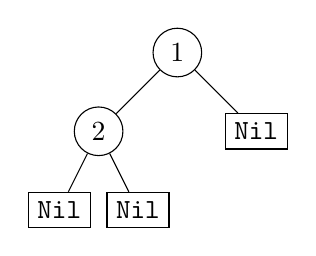
\begin{tikzpicture}
            \node[draw,circle] (A) at (0,0) {$1$};
            \node[draw,circle] (B) at (-1,-1) {$2$};
            \node[draw,rectangle] (C) at (1,-1) {\texttt{Nil}};
            \node[draw,rectangle] (D) at (-1.5,-2) {\texttt{Nil}};
            \node[draw,rectangle] (E) at (-0.5,-2) {\texttt{Nil}};
            \draw (A) -- (B) -- (D);
            \draw (A) -- (C);
            \draw (B) -- (E);
        \end{tikzpicture}
    \end{center}
    nous allons calculer son nombre de n\oe uds, en utilisant la fonction définie dans l'exercice précédent, dont on peut exprimer les règles d'induction de la façon suivante : 
    \begin{center}
        \begin{prooftree}
            \infer0{|\texttt{Nil}| = 0}
        \end{prooftree}
        \qquad
        \begin{prooftree}
            \hypo{|g| = k}
            \hypo{|d| = k'}
            \infer2{|\texttt{Node}(e,g,d)| = 1 + k + k'}
        \end{prooftree}
    \end{center}

    La dérivation est donc :
    \begin{center}
        \begin{prooftree}
            \infer0{|\texttt{Nil}| = 0}
            \infer0{|\texttt{Nil}| = 0}
            \infer2{|\texttt{Node}(2,\texttt{Nil},\texttt{Nil})| = 1 }
            \infer0{|\texttt{Nil}| = 0}
            \infer2{|A| = 2}
        \end{prooftree}
    \end{center}
\end{expl}


\begin{exo}
    Défnir les règles d'induction de la fonction $|-|$ sur les listes, associant à une liste sa longueur. \'Ecrire l'arbre de dérivation du calcul de $|[a,b,c]|$.
\end{exo}



\subsection{Relation inductive}

Intéressons-nous désormais aux relations entre objets inductifs. Comme précédemment, nous utiliserons des règles d'induction pour les définir (puisqu'une relation $\mathcal R$ peut être vue comme une fonction dans $\{0,1\}$), mais nous distinguerons deux types de prémisses : les prémisses du système formel et les prémisses \og meta\fg{}. Les premières sont celles qui interviennent directement dans les constructeurs de notre ensemble inductif, tandis que les deuxièmes sont des conditions que l'on peut dire extérieures à notre formalisme. Nous écrirons à côté de la règle les prémisses non syntaxiques (celles qui n'appartiennent pas au système formel). Attention cependant : nous nommerons souvent nos règles en donnant leur nom à droite de la barre, il faudra donc comprendre lorsqu'il y a une condition écrite à droite qu'elle est une prémisse non syntaxique, et lorsqu'il y a seulement un nom (par exemple $\to_e$) que c'est le nom de la règle.

\begin{expl}
    Nous allons définir le prédicat $P_k$ sur $\texttt{List}(\mathbb N)$ signifiant qu'une liste d'entiers possède un certain élément $k$ :
    \begin{center}\begin{prooftree}
        \hypo{}
        \infer1[$x = k$]{P_k(\texttt{cons}(x,l))}
    \end{prooftree}
    \qquad
    \begin{prooftree}
        \hypo{P_k(l)}
        \infer1{P_k(\texttt{cons}(x,l))}
    \end{prooftree}
    \end{center}
\end{expl}

\begin{exo}
    Montrer que $P_2([5,3,4,2,1,9])$ par un arbre de dérivation.
\end{exo}

\begin{rmk}
    On peut aussi définir des relations inductives mutuelles, par exemple un prédicat \og être pair\fg{} faisant appel à un prédicat \og être impair\fg{} faisant lui-même appel au premier prédicat (les deux ayant un cas de base), mais nous ne traiterons pas ce genre d'extension ici.
\end{rmk}

Donnons une définition de relation donnée par induction, car c'est un cas particulier qui nous sera utile.

\begin{defi}[Relation inductive]
    Soient $E,F$ deux ensembles. Soit un triplet $\langle C,\alpha,(D_c)_{c\in C}\rangle$ où $\alpha : C\to\nat, D_c : (E\times F)^{\alpha(c)}\to E\times F$ et $C$ est un ensemble. On dit que la relation $\mathcal R$ est définie par induction par ce triplet si $\mathcal R$ est la plus petite relation telle que pour tout $c\in C$, si pour tout $i \in\{0,\ldots,\alpha(c)\}, \mathcal R \langle x_i,y_i\rangle$ alors $\mathcal R(D_c(\langle x_1,y_1\rangle,\ldots,\langle x_{\alpha(c)},y_{\alpha(c)}\rangle))$. On note en général le triplet de la façon suivante : pour chaque $c\in C$, on écrit une règle de la forme
    \begin{center}
        \begin{prooftree}
            \hypo{\mathcal R(x_1,y_1)}
            \hypo{\mathcal R(x_2,y_2)}
            \hypo{\ldots}
            \hypo{\mathcal R(x_{\alpha(c)},y_{\alpha(c)})}
            \infer4[$c$]{\mathcal  R(D_c(\langle x_1,y_1\rangle,\ldots,\langle x_{\alpha(c)},y_{\alpha(c)}\rangle))}
        \end{prooftree}
    \end{center} avec $x_i,y_i$ non spécifiés, qu'il faut alors considérer comme quantifiée sur respectivement tout $E$ et tout $F$.
\end{defi}

\begin{exo}
    Montrer que si deux propositions sont stables par les règles définissant une relation inductive, alors l'intersection de ces propositions est aussi stable par ces règles. En déduire que la relation $\mathcal R$ définie par induction précédemment est l'intersection des propositions stables par les règles.
\end{exo}

\begin{exo}
    Montrer qu'une relation définie par induction par un ensemble de règles $\langle C,\alpha,(D_c)\rangle$ est non vide si et seulement s'il existe $c\in C$ tel que $\alpha(c) = 0$.
\end{exo}

\begin{rmk}
    Il arrivera que l'on écrive une règle dont les prémisses contiennent une ou des conditions qui ne sont pas de la forme $\mathcal R(x,y)$. Dans ce cas on peut considérer que l'on ajoute une règle de construction inductive pour chaque élément vérifiant cette prémisse et que le reste de la règle est paramétré par cet élément.
\end{rmk}

Nous pouvons maintenant réécrire notre théorème d'induction structurelle avec le formalisme des règles d'induction :

\begin{cor}[Preuve par induction]
    Soit une relation $\mathcal R$ entre deux ensembles $E,F$ générée par un ensemble de règles d'induction. Alors pour tout prédicat $P$ sur $E\times F$, pour montrer que $\mathcal R \subseteq P$ il suffit de montrer, pour chaque règle $c,\alpha(c),D_c$ définissant $\mathcal R$ la propriété suivante : pour tout $(x_1,\ldots,x_{\alpha(c)})\in P^{\alpha(c)}, P(D_c(x_1,\ldots,x_{\alpha(c)}))$, ce qui revient à montrer :
    \begin{center}
        \begin{prooftree}
            \hypo{P(x_1)}
            \hypo{P(x_2)}
            \hypo{\ldots}
            \hypo{P(x_{\alpha(c)})}
            \infer4[$c$]{P(D_c(x_1,\ldots,x_{\alpha(c)}))}
        \end{prooftree}
    \end{center}
\end{cor}

\begin{proof}
    C'est une conséquence directe du fait que $\mathcal R$ est définie comme la plus petite relation possédant cette propriété.
\end{proof}



\section{Définition des propositions}

Cette section vise à présenter les propositions, que nous introduirons comme des objets syntaxiques. La façon de séparer les propositions de leur interprétation (par exemple de dire que $\forall x. x = x$ n'est pas le même objet que $\top$) est une démarche qui se révélera fructueuse pour pouvoir trouver le bon formalisme pour parler de preuves et de valeur de vérité. On peut voir cela comme un analogue à la distinction entre un polynôme formel et une fonction polynomiale : le premier permet d'étudier de façon plus systématique le deuxième.

La première approche que nous aurons sera celle du calcul des propositions : on peut considérer une proposition (dans son sens intuitif) comme une phrase portant sur des objets mathématiques, par exemple avec la proposition $1 = 1$, auxquelles on associe des mots de liaison, comme $(1 = 1) \lor (0 = 1)$ indiquant que $1=1$ ou $0=1$. Cependant, on peut s'abstraire des prédicats de la forme $1=1$ et remplacer ceux-ci par une variable booléenne : une variable $x$ pouvant valoir $1$ (si elle représente une proposition atomique vraie) ou $0$ (si elle est fausse). Dans un second temps seulement, nous verrons le calcul des prédicats, permettant de parler plus précisément de ces propositions atomiques.

\subsection{Calcul des propositions}

\begin{defi}[Proposition]
    Soit un ensemble infini (dénombrable) de variables booléennes $\VV$ que nous noterons $x_1,x_2,\ldots$, nous définissons l'ensemble des propositions $\Prop$ par la grammaire suivante : $$ P,Q ::= x_i \mid \top\mid \bot \mid (P\to Q) \mid (P \lor Q) \mid (P\land Q)\mid (\lnot P)$$ où $\top$ et $\bot$ sont deux propositions atomiques constantes (appelées \og vrai\fg{} et \og absurde\fg{}).
\end{defi}

\begin{rmk}
    Un constructeur de cette grammaire est aussi appelé connecteur logique.
\end{rmk}

\begin{expl}
    Voici quelques propositions :
    \begin{itemize}[label=$\bullet$]
        \item $\top$
        \item $((\top \land (\lnot x_1))\lor (x_2\to x_3))$
    \end{itemize}
\end{expl}

\begin{rmk}
    Nous simplifierons l'écriture en rendant $\lnot$ le constructeur le plus prioritaire, $\lor$ et $\land$ prioritaire sur $\to$ et $\land$ prioritaire sur $\lor$ (le tout pour omettre un maximum de parenthèses). Par exemple la dernière proposition donnée en exemple peut se réécrire $\top\land \lnot x_1 \lor (x_2\to x_3)$. Enfin, l'opération $\to$ sera associative à droite : $x_0 \to x_1 \to x_2$ se lira $x_0 \to (x_1\to x_2)$.
\end{rmk}

Nous avons déjà une intuition assez naturelle de ce que veut dire chaque constructeur : par exemple, $P\land Q$ est vraie exactement lorsque $P$ et $Q$ à la fois sont vraies. Cette idée intuitive peut se formaliser par ce que l'on appelle des tables de vérité, représentant pour un connecteur la valeur de la proposition qu'il construit en fonction de la valeur de vérité de ses entrée. Voici les tables de vérité des différents connecteurs logiques :

{\begin{figure}[htb]
\centering
\begin{tabular}{|c|c|}
    \hline
     $P$ & $\lnot P$ \\ \hline\hline
     0 & 1 \\ \hline
     1 & 0 \\ \hline
\end{tabular}
\quad
\begin{tabular}{|c|c|c|}
    \hline
     $P$ & $Q$ & $P\to Q$ \\ \hline\hline
     0 & 0 & 1\\ \hline
     0 & 1 & 1\\ \hline
     1 & 0 & 0\\ \hline
     1 & 1 & 1\\ \hline
\end{tabular}
\quad
\begin{tabular}{|c|c|c|}
    \hline
     $P$ & $Q$ & $P\lor Q$  \\ \hline\hline
     0 & 0 & 0 \\ \hline
     0 & 1 & 1 \\ \hline
     1 & 0 & 1 \\ \hline
     1 & 1 & 1\\ \hline
\end{tabular}
\quad
\begin{tabular}{|c|c|c|}
    \hline
     $P$ & $Q$ & $P\land Q$ \\ \hline\hline
     0 & 0 & 0 \\ \hline
     0 & 1 & 0 \\ \hline
     1 & 0 & 0 \\ \hline
     1 & 1 & 1 \\ \hline
\end{tabular}
\caption{Tables de vérité}
\end{figure}}
\newpage

On peut alors essayer de donner une table de vérité pour n'importe quelle formule propositionnelle, mais les tables de vérité ont plusieurs inconvénients : elles sont longues à faire et elles sont difficiles à étudier mathématiquement. Nous leur préférerons donc la notion de valuation, que nous allons maintenant introduire.

\begin{defi}[Valuation]
    Soit une fonction $\nu : \VV \to \{0,1\}$ (qui à une variable associe si elle est vraie ou non), nous allons étendre par induction $\nu$ en une fonction $\nu^*:\Prop \to \{0,1\}$ par les règles suivantes :
    \begin{center}
        \begin{prooftree}
            \infer0[$\top$]{\nu^*(\top)=1}
        \end{prooftree}
        \quad
        \begin{prooftree}
            \infer0[$\bot$]{\nu^*(\bot)=0}
        \end{prooftree}
        \quad
        \begin{prooftree}
            \infer0[Ax]{\nu^*(x_i) = \nu(x_i)}
        \end{prooftree}
        \\
        \vspace{0.5cm}
        \begin{prooftree}
            \hypo{\nu^*(P) = b}
            \infer1[$\lnot$]{\nu^*(\lnot P) = 1 - b}
        \end{prooftree}
        \quad
        \begin{prooftree}
            \hypo{\nu^*(P) = b_1}
            \hypo{\nu^*(Q) = b_2}
            \infer2[$\to$]{\nu^*(P\to Q) = 1-b_1+b_1\times b_2}
        \end{prooftree}\\
        \vspace{0.5cm}
        \begin{prooftree}
            \hypo{\nu^*(P) = b_1}
            \hypo{\nu^*(Q) = b_2}
            \infer2[$\lor$]{\nu^*(P\lor Q) = b_1 + b_2 - b_1\times b_2}
        \end{prooftree}
        \quad
        \begin{prooftree}
            \hypo{\nu^*(P) = b_1}
            \hypo{\nu^*(Q) = b_2}
            \infer2[$\land$]{\nu^*(P\land Q) = b_1\times b_2}
        \end{prooftree}
    \end{center}
\end{defi}

\begin{rmk}
    Les opérations utilisées pour les valuations de $P\to Q$ et $P\lor Q$ sont un peu longues, mais elles correspondent simplement à leur table de vérité.
\end{rmk}

\begin{exo}
    Montrer par une dérivation que chaque table de vérité est vérifiée avec notre définition de $\nu^*$.
\end{exo}

\begin{exo}
    Montrer que deux valuations $\nu,\nu'$ donnent la même valeur sur une proposition $P$ si pour toute variable $x_i$ intervenant dans $P$, $\nu(x_i)=\nu'(x_i)$.
\end{exo}

On peut donc se restreindre aux valuations $\nu$ partielles, c'est-à-dire n'associant qu'un nombre fini de valeurs à l'ensemble $\VV$, dont le domaine contient les variables intervenant dans une proposition $P$, pour évaluer $P$.

\begin{expl}
    Soit la proposition $P := x_0\lor x_1 \to x_2$, et la valuation $$\nu : x_0 \mapsto 0, x_1 \mapsto 1, x_2 \mapsto 0$$ on peut alors calculer $\nu^*(P)$ :
    \begin{center}
        \begin{prooftree}
            \infer0[Ax]{\nu^*(x_0)=0}
            \infer0[Ax]{\nu^*(x_1)=1}
            \infer2[$\lor$]{\nu^*(x_0\lor x_1) = 1}
            \infer0[Ax]{\nu^*(x_2)=0}
            \infer2[$\to$]{\nu^*(x_0\lor x_1 \to x_2) = 0}
        \end{prooftree}
    \end{center}
\end{expl}

Si l'on considère que $1$ signifie que la proposition est vraie et que $0$ signifie que la proposition est fausse, on peut donc dire qu'une proposition est vraie pour une certaine valuation. 

\begin{defi}[Modèle d'une proposition]
    Soit $\nu$ une valuation. On dit que $P$ est vraie (ou satisfaite) pour la valuation $\nu$, ou encore que $\nu$ est modèle de $P$, et on note $\nu\models P$, si $\nu^*(P) = 1$.
\end{defi}

\begin{defi}[Tautologie]
    On dit que $P$ est une tautologie si pour toute valuation $\nu$, $\nu^*\models P$.
\end{defi}

Par la suite, on confondra directement $\nu$ et $\nu^*$.

\subsection{Satisfiabilité et compacité}

\'Etendons maintenant notre notion de vérité pour un ensemble de propositions :

\begin{defi}[Satisfiabilité]
    On dit qu'une formule $P$ est satisfiable s'il existe une valuation $\nu$ telle que $\nu\models P$.

    Si $\mathbf{P}\subseteq \Prop$ est un ensemble de proposition, alors on dit que $\mathbf{P}$ est satisfiable s'il existe une valuation $\nu$ telle que pour tout $P\in\mathbf{P}$, $\nu\models P$. On note alors $\nu\models \textbf{P}$.
\end{defi}

\begin{rmk}
    Cette digression est hors du cadre de ce document, mais le problème de trouver, étant donnée une proposition, si elle est satisfiable, est un problème dit NP-complet. Il est historiquement le premier problème démontré comme étant NP-complet et revêt en ce sens une importance primordiale en théorie de la complexité algorithmique.
\end{rmk}

Donnons aussi la définition d'un ensemble contradictoire :

\begin{defi}[Ensemble contradictoire]
    Un ensemble $\mathbf P\subseteq \mathcal P$ (potentiellement infini) est contradictoire s'il n'existe pas de valuation $\nu$ telle que $\nu\models \mathbf P$.
\end{defi}

Le calcul des propositions n'est malheureusement pas le plus pertinent, car il manque à ce système deux éléments essentiels : pouvoir s'appliquer à des objets mathématiques et pouvoir introduire des quantifications. Nous nous contenterons donc de donner un théorème central de la logique : le théorème de compacité.

\begin{defi}[Ensemble finiment satisfiable, contradictoire]
    Soit $\mathbf{P}$ un ensemble (infini) de propositions, on dit que $\mathbf{P}$ est finiment satisfiable si pour toute partie finie $P\subseteq_{\mathrm{fin}}\mathbf P$, $P$ est satisfiable.
    
    De même, $\mathbf P$ est dite finiment contradictoire s'il existe une partie finie de $\mathbf P$ qui est contradictoire.
\end{defi}

\begin{them}[Compacité de la logique propositionnelle]
    Soit $\mathbf P$ un ensemble de propositions. Alors $\mathbf P$ est satisfiable si et seulement si $\mathbf P$ est finiment satisfiable.
\end{them}

\begin{proof}
    Il est évident qu'un ensemble satisfiable est finiment satisfiable, le théorème tient bien sûr dans le sens réciproque.

    Soit un ensemble de propositions $\mathbf P$. Nous allons définir une suite $(\varepsilon_n)$ qui définira notre valuation par $\nu(x_n)=\varepsilon_n$. Cette construction se fera par induction :
    \begin{itemize}[label=$\bullet$]
        \item Tout d'abord, deux cas sont possibles :
        \begin{enumerate}
            \item\label{cas1} pour tout sous-ensemble fini $B$, il existe une valuation $\delta$ satisfiant $B$ et telle que $\delta(x_0)=0$ : dans ce cas on définit $\varepsilon_0 = 0$.
            \item\label{cas2} il existe un sous-ensemble fini $B_0$ tel que pour toute valuation $\delta$ satisfiant $B_0$, $\delta(x_0)=1$ : dans ce cas on définit $\varepsilon_0 = 1$.
        \end{enumerate} 
        \item Montrons l'initialisation de la propriété \og il existe une suite $\varepsilon_0,\ldots,\varepsilon_n$ telle que pour tout sous-ensemble $B$ il existe un valuation $\delta$ satisfaisant $B$ et telle que $\delta(x_i)=\varepsilon_i$\fg{} : dans le cas \ref{cas1}, le résultat est direct. Dans le cas \ref{cas2}, alors pour une partie finie $B$ on considère $B\cup B_0$ : si $\delta\models B\cup B_0$ alors $\delta\models B_0$ donc $\delta(x_0)=1$ et $\delta\models B$, donc notre hypothèse est vérifiée.
        \item Supposons qu'il existe une suite $\varepsilon_0,\ldots,\varepsilon_n$ vérifiant les conditions énoncées, alors on peut encore séparer deux cas :
        \begin{enumerate}
            \item pour toute partie finie $B$ il existe une valuation $\delta\models B$ telle que $\delta(x_i)=\varepsilon_i$ pour $i\leq n$, on a aussi $\delta(x_{n+1})=0$.
            \item il existe une partie finie $B_{n+1}$ telle que pour toute valuation $\delta\models B$ telle que $\delta(x_i) =\varepsilon_i$ pour $i\leq n$, on a $\delta(x_{n+1})=1$.
        \end{enumerate}
        Dans le premier cas, on définit $\varepsilon_{n+1}=0$ et l'hérédité est vérifiée, et dans le deuxième cas on définir $\varepsilon_{n+1}=1$ et alors pour $B$ une partie finie, il existe $\delta\models B \cup B_{n+1}$ avec $\delta(x_i)=\varepsilon_i$ pour $i\leq n$, et comme $\delta\models B_{n+1}$ on en déduit qu'il existe $\delta\models B$ avec $\delta(x_i) =\varepsilon_i$ pour $i\leq n+1$.
    \end{itemize}

    Ainsi, par récurrence, nous avons défini la valuation $\nu : x_i \mapsto \varepsilon_i$ qui satisfait toute proposition de $\mathbf P$.
\end{proof}

\begin{exo}[Formulation équivalente du théorème de compacité]
    Montrer que le théorème de compacité équivaut au théorème suivant : tout ensemble est contradictoire si et seulement s'il est finiment contradictoire.
\end{exo}


\section{Liens entre syntaxe et sémantique}

Nous avons défini, dans notre syntaxe, le connecteur $\to$, qui se traduit en général par \og $P\to Q$ signifie que $Q$ est une conséquence logique de $P$\fg{}. Cependant, ce connecteur ne possède pas de sens en lui-même : il n'a de sens qu'à travers notre règle d'induction pour la définition de $\nu^*$, car c'est bien le comportement des connecteurs vis à vis des valuations qui détermine le sens de ces connecteurs (plus précisément : le sens est donné par les valuations, c'est pour cela qu'on considère que celles-ci sont un aspect sémantique de notre logique, là où les suites de symboles que sont les propositions sont purement syntaxiques). Cependant, de par la forme des propositions, on peut établir un système qui, sans utiliser de valuations, va pouvoir exprimer des notions de conséquence (entre autres choses).

\begin{defi}[Conséquence sémantique]
    Soit $\mathbf P\subseteq\mathcal P$ un ensemble de proposition et $P$ une proposition, on dit que $P$ est conséquence sémantique de $\mathbf P$ si pour toute valuation $\nu\models\mathbf P$, on a $\nu\models P$. 
\end{defi}

\begin{expl}
    Il est évident que si $P\in\mathbf P$, alors $P$ est conséquence sémantique de $\mathbf P$. On peut aussi montrer que si $P\in\mathbf P$ et $Q\in\mathbf P$ alors $P\land Q$ est conséquence sémantique de $\mathbf P$.
\end{expl}

\begin{exo}
    Montrer qu'une formulation équivalente du théorème de compacité est la suivante : une proposition $P$ est conséquence sémantique d'un ensemble de propositions $\mathbf P$ si et seulement si elle est conséquence sémantique d'une partie finie de $\mathbf P$.
\end{exo}

\subsection{Déduction naturelle avec présentation en séquents}

A partir de nos exemples se dessine un schéma de règles assez naturel : pour un ensemble de propositions, on peut directement dériver des propositions qui en sont des conséquences sémantiques, sans avoir à raisonner réellement sur les valuations. Nous allons donc définir un système syntaxique appelé déduction naturelle permettant de formaliser cette idée.

\begin{defi}[Séquent en déduction naturelle]
    Soit $\Gamma$ un ensemble de propositions (présenté sous forme de liste) et $P$ une propositions, on note $\Gamma\vdash P$, et on lit \og gamma thèse $P$\fg{} le séquent exprimant que $P$ peut se déduire des hypothèses $\Gamma$. Ceci constitue une relation inductive dont les règles de constructions sont précisées dans la figure \ref{fig:deducnat} ci-dessous.
\end{defi}

\begin{figure}[htb]
    \centering
    \rule{17cm}{0.5pt}\\
    \vspace{0.5cm}
    \begin{prooftree}
        \infer0[$\top_\mathrm{i}$]{\Gamma\vdash \top}
    \end{prooftree}
    \quad
    \begin{prooftree}
        \infer0[Ax]{\Gamma,P\vdash P}
    \end{prooftree}
    \quad
    \begin{prooftree}
        \hypo{\Gamma,P\vdash Q}
        \infer1[$\to_\mathrm i$]{\Gamma\vdash P\to Q}
    \end{prooftree}
    \quad
    \begin{prooftree}
        \hypo{\Gamma\vdash P\to Q}
        \hypo{\Gamma\vdash P}
        \infer2[$\to_\mathrm e$]{\Gamma\vdash Q}
    \end{prooftree}
    \\
    \vspace{0.5cm}
    \begin{prooftree}
        \hypo{\Gamma\vdash P}
        \hypo{\Gamma\vdash Q}
        \infer2[$\land_\mathrm i$]{\Gamma\vdash P\land Q}
    \end{prooftree}
    \quad
    \begin{prooftree}
        \hypo{\Gamma\vdash P\land Q}
        \infer1[$\land_\mathrm e^\mathrm g$]{\Gamma\vdash P}
    \end{prooftree}
    \quad
    \begin{prooftree}
        \hypo{\Gamma\vdash P\land Q}
        \infer1[$\land_\mathrm e^\mathrm d$]{\Gamma\vdash Q}
    \end{prooftree}
    \\
    \vspace{0.5cm}
    \begin{prooftree}
        \hypo{\Gamma\vdash P}
        \infer1[$\lor_\mathrm i^\mathrm g$]{\Gamma\vdash P \lor Q}
    \end{prooftree}
    \quad
    \begin{prooftree}
        \hypo{\Gamma\vdash Q}
        \infer1[$\lor_\mathrm i^\mathrm d$]{\Gamma\vdash P \lor Q}
    \end{prooftree}
    \quad
    \begin{prooftree}
        \hypo{\Gamma\vdash P \lor Q}
        \hypo{\Gamma,P\vdash C}
        \hypo{\Gamma,Q\vdash C}
        \infer3[$\lor_\mathrm e$]{\Gamma\vdash C}
    \end{prooftree}
    \\
    \vspace{0.5cm}
    \begin{prooftree}
        \hypo{\Gamma,A\vdash \bot}
        \infer1[$\lnot_\mathrm i$]{\Gamma\vdash \lnot A}
    \end{prooftree}
    \quad
    \begin{prooftree}
        \hypo{\Gamma\vdash A}
        \hypo{\Gamma\vdash \lnot A}
        \infer2[$\lnot_\mathrm e$]{\Gamma\vdash \bot}
    \end{prooftree}
    \quad
    \begin{prooftree}
        \hypo{\Gamma,\lnot A\vdash \bot}
        \infer1[$\bot_\mathrm c$]{\Gamma\vdash A}
    \end{prooftree}
    \\
    \vspace{0.5cm}
    \rule{17cm}{0.5pt}
    \caption{Règles de la déduction naturelle}
    \label{fig:deducnat}
\end{figure}

\begin{rmk}
    On appelle un arbre de preuve une dérivation, à partir de ces règles, d'un séquent.

    Si $\Gamma=\varnothing$, on notera directement $\vdash P$.
\end{rmk}

\begin{expl}
Voici un exemple de dérivation de $P\to P$ :
\begin{center}
    \begin{prooftree}
        \infer0[Ax]{P\vdash P}
        \infer1[$\to_\mathrm i$]{\vdash P \to P}
    \end{prooftree}
\end{center}
\end{expl}

\begin{exo}
    Pour chaque proposition, construire un arbre de preuve :
    \begin{itemize}[label=$\bullet$]
        \item $\vdash P \to Q \to P$
        \item $\vdash (P \to Q \to R) \to (P \to Q) \to P \to R$
        \item $(P\lor Q)\land R\vdash (P\land R)\lor (Q\land R)$
        \item $\lnot\lnot A \to A$
        \item $\lnot A \lor A$
    \end{itemize}
\end{exo}

\begin{exo}[Principe d'explosion]
    Une règle importante en logique, nommée \textit{ex falso quodlibet}, stipule que si l'on prouve $\bot$ (la formule fausse) alors on peut prouver n'importe quoi, elle s'écrit \begin{center}
        \begin{prooftree}
            \hypo{\Gamma\vdash \bot}
            \infer1[$\bot_\mathrm i$]{\Gamma\vdash A}
        \end{prooftree}
    \end{center}
    Montrer que $\bot_\mathrm i$ est dérivable, c'est-à-dire que l'on peut construire un arbre partant de la prémisse de la règle pour arriver à sa conclusion (la lettre i pour désigner cette règle fait référence à l'intuitionnisme, car cette règle remplace $\bot_\mathrm c$, l'absurde classique, en logique intuitionniste).
\end{exo}

Nous pouvons remarquer que chaque règle d'induction correspond à une règle logique évidente :
\begin{itemize}[label=$\bullet$]
    \item La règle $\top_\mathrm i$ dit simplement que l'on peut toujours déduire la formule vraie.
    \item La règle Ax dit que l'on peut déduire $P$ directement si l'on a fait l'hypothèse $P$.
    \item La règle $\to_\mathrm i$ dit que pour montrer $P\to Q$ il suffit de supposer $P$ pour montrer $Q$.
    \item La règle $\to_\mathrm e$, aussi appelée \textit{modus ponens}, dit que si l'on a prouvé $P\to Q$ et $P$, alors on peut en déduire $Q$.
    \item Les règles liées à $\lor$, $\land$ et $\lnot$ sont assez lisibles, à l'exception de $\lor_\mathrm e$ : elle correspond à la disjonction de cas. En effet, si l'on a prouvé $P\lor Q$, alors prouver $C$ revient à le prouver sous l'hypothèse $P$ et sous l'hypothèse $Q$.
    \item La règle $\bot_\mathrm c$, appelée raisonnement par l'absurde, permet de déduire $A$ du fait que $\lnot A$ mène à une contradiction.
\end{itemize}

L'exercice suivant est un résultat de structure de notre système, qui sera utile par la suite :

\begin{exo}[Affaiblissement]
    Montrer par induction que s'il existe une dérivation de $\Gamma\vdash P$ alors pour toute proposition $A$, il existe une dérivation de $\Gamma,A\vdash P$ (ceci signifie que si l'on a prouvé un résultat, on peut encore le prouver en rajoutant des hypothèses).
\end{exo}

\begin{exo}[Codage de la négation]
    Montrer que le séquent suivant est dérivable : $$\vdash (\lnot P \to (P\to\bot))\land((P\to\bot)\to\lnot P)$$
\end{exo}

\subsection{Correction et complétude du calcul propositionnel}

Ces règles paraissent dont très convaincantes pour créer un formalisme robuste de raisonnement. Pourtant, ce ne sont que des règles formelles : des enchaînements de symboles qui n'ont \textit{a priori} pas de lien avec la sémantique de nos propositions. Heureusement, il existe une paire de théorème nous permettant d'établir l'équivalence entre la conséquence sémantique et la conséquence syntaxique (c'est-à-dire le fait de prouver $\Gamma\vdash P$).

\begin{them}[Correction du calcul propositionnel]
    Si $\Gamma\vdash P$ pour $\Gamma$ un ensemble de propositions, alors $P$ est conséquence sémantique de $\Gamma$, i.e. pour toute valuation $\nu$, si $\nu\models\Gamma$ alors $\nu\models P$.
\end{them}

\begin{proof}
    La preuve se fait par induction sur $\Gamma\vdash P$, il suffit donc de montrer que pour chaque règle, si le théorème est vrai pour ses prémisses, alors il est vrai pour sa conclusion. Nous laissons en exercice au lecteur le traitement de la plupart des règles, mais donnerons le traitement de deux règles pour l'exemple :
    \begin{itemize}[label=$\bullet$]
        \item Cas de $\to_\mathrm e$ : supposons que $\Gamma\vdash P\to Q$ et $\Gamma\vdash P$, et de plus que cela $P\to Q$ et $P$ sont conséquences sémantiques de $\Gamma$ (par hypothèse d'induction), montrons qu'alors $Q$ est conséquence sémantique de $\Gamma$. Soit $\nu$ satisfaisant $\Gamma$, alors par hypothèse, $\nu(P) = 1$ et $\nu(P\to Q)=1$, or $\nu(P\to Q) = 1 - \nu(P)+\nu(P)\nu(Q)$ donc en simplifiant, on en déduit que $\nu(Q) = 1$ : donc $Q$ est conséquence sémantique de $\Gamma$.
        \item Cas de $\lor_\mathrm e$ : on suppose donc que $P\lor Q$ est conséquence sémantique de $\Gamma$, que $C$ est conséquence sémantique de $\Gamma,P$ et de $\Gamma,Q$, et on veut montrer que $C$ est conséquence sémantique de $\Gamma$. Soit $\nu$ satisfaisant $\Gamma$, alors $\nu(P\lor Q) = 1$, c'est-à-dire $\nu(P)+\nu(Q)-\nu(P)\nu(Q)=1$. Alors soit $\nu(P)=1$, soit $\nu(Q)=1$ (possiblement les deux). Supposons sans perte de généralité que $\nu(P)=1$ : cela signifie que $\nu$ satisfait $\Gamma,P$, donc comme $C$ est conséquence logique de $\Gamma,P$, $\nu(C)=1$. Donc $C$ est conséquence logique de $\Gamma$. 
    \end{itemize}
\end{proof}

\begin{exo}
    Montrer le théorème pour les autre règles d'induction.
\end{exo}

Ce théorème nous dit donc que ce qu'on prouve avec ces règles est correct. La question naturelle qui s'ensuit est \og peut-on prouver tout ce qui est vrai ?\fg{} Il se trouve que c'est le cas, c'est ce que montre le prochain théorème.

Pour préparer ce résultat, nous aurons besoin d'une suite de lemmes (le premier sera ici donné en exercice). Ces lemmes ont des preuves principalement techniques et il est conseillé pour le lecteur de ne pas s'attarder sur celles-ci.

\begin{exo}
    Montrer que $P$ est conséquence sémantique d'un ensemble fini de propositions $\Gamma$ si et seulement si $\left(\displaystyle{\bigwedge_{\gamma\in\Gamma}}\gamma \right)\to P$ est une tautologie. Où cette notation signifie que l'on considère la conjonction (connecteur \og et\fg{}) sur toutes les formules de $\Gamma$.
\end{exo}

Nous allons construire, pour une valuation $\nu$, une proposition permettant de représenter, en quelque sorte, $\nu$. La preuve se basera sur le fait que $\nu\models P$ pourra s'interpréter comme $\vdash \nu\to P$.

\begin{lem}
    Soit $P$ une proposition et $\nu$ une valuation sur les variables de $P$, on note $V(\nu)$ une proposition correspondant à une conjonction contenant toutes les propositions $x_i$ telles que $\nu(x_i)=1$ et les négations des propositions $x_j$ telles que $\nu(x_j) = 0$. Par exemple pour $\nu(x_0)=1,\nu(x_1)=0$ on a au moins $V(\nu) = x_0\land \lnot x_1$. Alors :
    \begin{itemize}[label=$\bullet$]
        \item soit $\nu(P) = 1$ et alors $V(\nu) \vdash P$
        \item soit $\nu(P) = 0$ et alors $V(\nu) \vdash \lnot P$.
    \end{itemize}
\end{lem}

\begin{proof}
    Procédons par induction sur $P$ :
    \begin{itemize}[label=$\bullet$]
        \item Les cas $\top$ et $\bot$ sont évidents, puisqu'ils ne font pas intervenir de variables.
        \item Cas $x_i$ : soit $V(\nu)$ avec $\nu$ une valuation sur $x_i$. Supposons que $\nu(x_i)=1$. Alors \begin{center}
            \begin{prooftree}
                \infer0[Ax]{V(\nu)\vdash V(\nu)}
                \infer1[$\land_\mathrm e$]{V(\nu)\vdash x_i}
            \end{prooftree}
        \end{center} où l'on note $\land_\mathrm e$ pour choisir le $x_i$ précis dans $V(\nu)$ (on peut se convaincre qu'une suite finie d'applications de $\land_\mathrm e$ permet de faire ceci). La preuve est la même si $\nu(x_i) = 0$ (on obtiendra simplement $\lnot x_i$ à la place).
        \item Cas $\lor$ : soit $\nu$ une valuation contenant les variables de $P$ et de $Q$, et $V(\nu)$ une proposition associée à $\nu$. Quatre cas peuvent alors arriver, mais nous ne traiterons que deux d'entre eux (le lectuer assidu vérifiera les autres) : si $\nu(P)=1$ et $\nu(Q)=0$ (et donc que $\nu(P\lor Q) = 1$) alors on sait que $V(\nu)\vdash P$ et $V(\nu)\vdash \lnot Q$. On construit alors :
        \begin{center}
            \begin{prooftree}
                \hypo{V(\nu)\vdash P}
                \infer1[$\lor_\mathrm i$]{V(\nu)\vdash P\lor Q}
            \end{prooftree}
        \end{center}
        Si $\nu(P)=\nu(Q)=0$ alors $V(\nu)\vdash \lnot P$, $V(\nu)\vdash \lnot Q$ et on veut montrer que $V(\nu)\vdash \lnot (P\lor Q)$ :
        \begin{center}
        \scalebox{0.7}{
            \begin{prooftree}
                \infer0[Ax]{V(\nu),P\lor Q\vdash P\lor Q}
                \hypo{V(\nu),P\lor Q,P\vdash \lnot P}
                \infer0[Ax]{V(\nu),P\lor Q,P\vdash P}
                \infer2[$\lnot_\mathrm e$]{V(\nu),P\lor Q,P\vdash \bot}
                \hypo{V(\nu),P\lor Q,Q\vdash \lnot Q}
                \infer0[Ax]{V(\nu),P\lor Q,Q\vdash Q}
                \infer2[$\lnot_\mathrm e$]{V(\nu),P\lor Q,Q\vdash \bot}
                \infer3[$\lor_\mathrm e$]{V(\nu),P\lor Q\vdash\bot}
                \infer1[$\lnot_\mathrm i$]{V(\nu)\vdash \lnot (P\lor Q)}
            \end{prooftree}
        }
        \end{center}
        \item Cas $\land$ : soit $\nu$ une valuation contenant les variables de $P$ et de $Q$ et $V(\nu)$ une proposition associée à $\nu$. Là encore, quatre cas sont possibles. Si $\nu(P)=\nu(Q)=0$ alors par hypothèse d'induction $V(\nu)\vdash \lnot P$, $V(\nu)\vdash \lnot Q$, et alors :
        \begin{center}
            \begin{prooftree}
                \hypo{V(\nu),P\land Q\vdash \lnot P}
                \infer0[Ax]{V(\nu),P\land Q\vdash P\land Q}
                \infer1[$\land_\mathrm e^\mathrm g$]{V(\nu),P\land Q\vdash P}
                \infer2[$\lnot_\mathrm e$]{V(\nu),P\land Q\vdash \bot}
                \infer1[$\lnot_\mathrm i$]{V(\nu)\vdash \lnot(P\land Q)}
            \end{prooftree} 
        \end{center}
        Si $\nu(P)=0$ et $\nu(Q) = 1$, remarquons que l'arbre plus haut est encore parfaitement utilisable puisque $\nu(P\land Q) = 0$. De même en inversant les rôles de $P$ et $Q$, on peut prouver le cas où $\nu(P)=1$ et $\nu(Q)=0$. Enfin, si $\nu(P)=\nu(Q)=1$ :
        \begin{center}
            \begin{prooftree}
                \hypo{V(\nu)\vdash P}
                \hypo{V(\nu)\vdash Q}
                \infer2[$\land_\mathrm i$]{V(\nu)\vdash P\land Q}
            \end{prooftree}
        \end{center}
        \item Cas $\lnot$ : soit $\nu$ une valuation contenant les variables de $P$, et $V(\nu)$ une proposition associée. Si $\nu(P) = 1$ alors $\nu(\lnot(P))=0$, on veut donc montrer qu'à partir de $V(\nu)\vdash P$ on peut déduire $V(\nu)\vdash \lnot\lnot P$ :
        \begin{center}
            \begin{prooftree}
                \hypo{V(\nu),\lnot P\vdash P}
                \infer0[Ax]{V(\nu),\lnot P\vdash \lnot P}
                \infer2[$\lnot_\mathrm e$]{V(\nu),\lnot P\vdash \bot}
                \infer1[$\lnot_\mathrm i$]{V(\nu)\vdash \lnot \lnot P}
            \end{prooftree}
        \end{center}
        Si $\nu(P)=0$, alors on veut montrer qu'à partir de $V(\nu)\vdash \lnot P$ on peut en déduire que $V(\nu)\vdash \lnot P$, ce qui est évident.
        \item Cas $\to$ : soit $\nu$ une valuation contenant les variables de $P$ et $Q$, et $V(\nu)$ une proposition associée. Il reste encore quatre cas à traiter. Si $\nu(P)=\nu(Q)=0$, alors on veut montrer que $V(\nu)\vdash P\to Q$ à partir de $V(\nu)\vdash \lnot P$ et $V(\nu)\vdash \lnot Q$ :
        \begin{center}
            \begin{prooftree}
                \hypo{V(\nu),P\vdash \lnot P}
                \infer0[Ax]{V(\nu),P\vdash P}
                \infer2[$\lnot_\mathrm e$]{V(\nu),P\vdash\bot}
                \infer1[$\bot_\mathrm i$]{V(\nu),P\vdash Q}
                \infer1[$\to_\mathrm i$]{V(\nu)\vdash P\to Q}
            \end{prooftree}
        \end{center}
        Remarquons que nous n'avons, là encore, pas eu besoin d'utiliser l'hypothèse sur $Q$. On peut donc traiter avec le même arbre le cas où $\nu(P)=0$ et $\nu(Q)=1$. Si $\nu(P) = 1$ et $\nu(Q)=0$, il nous faut prouver $V(\nu)\vdash \lnot (P\to Q)$ avec les hypothèses $V(\nu)\vdash P$ et $V(\nu)\vdash \lnot Q$ :
        \begin{center}
            \begin{prooftree}
                \hypo{V(\nu),P\to Q\vdash \lnot Q}
                \hypo{V(\nu),P\to Q\vdash P}
                \infer0[Ax]{V(\nu),P\to Q\vdash P \to Q}
                \infer2[$\to_\mathrm e$]{V(\nu),P\to Q\vdash Q}
                \infer2[$\lnot_\mathrm e$]{V(\nu),P\to Q\vdash \bot}
                \infer1[$\lnot_\mathrm i$]{V(\nu)\vdash \lnot (P\to Q)}
            \end{prooftree}
        \end{center}
        Enfin, si $\nu(P)=\nu(Q)=1$, alors par $\to_\mathrm i$ on déduit de $V(\nu),P\vdash Q$ que $V(\nu)\vdash P\to Q$.
    \end{itemize}
\end{proof}

\begin{lem}
    Soit $P$ une proposition. Si $P$ est une tautologie, alors $\vdash P$.
\end{lem}

\begin{proof}
    Procédons par récurrence sur l'indice maximal des variables présentes dans $P$ :
    \begin{itemize}[label=$\bullet$]
        \item Si la seule variable apparaissant dans $P$ est $x_0$, alors comme $P$ est une tautologie et par le lemme précédent, on sait que $x_0\vdash P$ et $\lnot x_0\vdash P$, ce qui nous permet de déduire que $\vdash P$ (en utilisant un exercice précédent où l'on a montré que $\vdash A\lor\lnot A$) :
        \begin{center}
            \begin{prooftree}
                \hypo{\vdash x_0\lor\lnot x_0}
                \hypo{x_0\vdash P}
                \hypo{\lnot x_0\vdash P}
                \infer3[$\lor_\mathrm e$]{\vdash P}
            \end{prooftree}
        \end{center}
        \item Supposons que pour toute proposition faisant intervenir des variables jusqu'à $i$, être une tautologie implique d'être dérivable dans notre système. Soit alors une proposition $P$ faisant intervenir des variables jusqu'à $i+1$. Soit $\nu$ une valuation sur les $i$ premières variables. Comme $P$ est une tautologie, alors $P$ est satisfaite par $\nu'$ valant $\nu$ jusqu'à $x_i$ et $1$ en $x_{i+1}$, et par $\nu''$ valant $\nu$ jusqu'à $x_i$ et $0$ en $x_{i+1}$. On en déduit donc que $V(\nu')\vdash P$ et $V(\nu'')\vdash P$, soit $V(\nu)\land x_{i+1}\vdash P$ et $V(\nu)\land \lnot x_{i+1}\vdash P$. Par introductions successives de l'implication, on a alors $x_{i+1}\vdash V(\nu)\to P$ et $\lnot x_{i+1}\vdash V(\nu)\to P$, nous ramenant (en utilisant le même raisonnement que le cas précédent) à $\vdash V(\nu)\to P$, ce qui revient à $V(\nu)\vdash P$ qui est dérivable par le lemme précédent.
    \end{itemize}

    Donc par induction, $\vdash P$.
\end{proof}

\begin{rmk}
    Nous avons ici utilisé que si $P\land Q \vdash R$ alors $Q\vdash P\to R$. Ceci n'est pas une règle de à proprement parler, mais on peut prouver ce résultat par induction sur les arbres de preuve. Cela peut faire un exercice, mais il est surtout fastidieux et l'idée est principalement que l'on peut remplacer $P\land Q\vdash R$ par $P,Q\vdash R$ en remplaçant chaque utilisation de l'axiome pour $P$ ou pour $Q$ par un axiome pour $P\land Q$ puis une élimination du $\land$. Nous pouvons le statuer comme une sorte de meta-règle (qui nous permet de dire qu'un séquent est dérivable à partir d'un autre séquent qui est dérivable), qu'on appelle une règle admissible.
\end{rmk}

\begin{them}[Complétude du calcul propositionnel]
    Soit $\Gamma$ un ensemble de propositions et $P$ une proposition. Si $P$ est conséquence sémantique de $\Gamma$, i.e. pour toute valuation $\nu$, si $\nu\models\Gamma$ alors $\nu\models P$, alors $\Gamma\vdash P$.
\end{them}

\begin{proof}
    Sous nos hypothèses, avec le théorème de compacité, on peut considérer une partie finie $\Gamma_0\subseteq\Gamma$ telle que $P$ en est conséquence sémantique. On veut donc prouver que $\Gamma_0\vdash P$, ce qui revient à montrer que $\vdash \left(\displaystyle{\bigwedge_{\gamma\in\Gamma_0}}\gamma \right)\to P$, et la condition sémantique est équivalente à dire que $\left(\displaystyle{\bigwedge_{\gamma\in\Gamma_0}}\gamma \right)\to P$ est une tautologie. Nous n'avons donc à montrer que le résultat (plus faible) suivant : si $P$ est une tautologie, alors $\vdash P$ est dérivable. C'est justement le résultat du lemme précédent.
\end{proof}

\begin{exo}[\'Enoncé équivalent du théorème de complétude]
    Montrer que le théorème de complétude revient à l'énoncé suivant : si $\Gamma$ est contradictoire, alors $\Gamma\vdash \bot$.
\end{exo}

Nous savons maintenant qu'avec notre système de calcul, la preuve syntaxique et la correspondance sémantique sont équivalentes. Ainsi, être conséquence sémantique ou syntaxique correspond à la même chose, d'où la  définition suivante :

\begin{defi}[Conséquence, équivalence]
    On dit qu'une proposition $Q$ est conséquence d'une proposition $P$ si l'un des conditions équivalentes est vérifiées : $P\vdash Q$ ; $Q$ est conséquence sémantique de $P$ ; $\vdash P \to Q$ ; $P\to Q$ est une tautologie. On notera parfois cela $P\implies Q$ (mais on évitera en général de le faire pour ne pas confondre avec $\to$, qui est un connecteur logique, là où $\implies$ représente donc une méta-proposition, une propriété sur nos propositions elles-mêmes).

    On dit que deux propositions $P$ et $Q$ sont équivalentes lorsque $P$ est conséquence de $Q$ et $Q$ est conséquence de $P$. On notera alors $P\iff Q$ ou $P\equiv Q$ (la deuxième notation sera privilégiée).
\end{defi}



\section{Algèbres de Boole}

Le calcul propositionnel nous a donné un formalisme pour parler de propositions, de vérité et de preuves. Nous avons vu que les éléments essentiels du calcul propositionnels sont les constructeurs (c'est-à-dire $\lor$,$\land$,$\to$,$\lnot$) des propositions, puisque ce calcul ne s'intéresse qu'au lien entre les propositions. Ceci motive alors l'étude des algèbres de Boole, qui sont des structures se comportant de la même façon : elles possèdent des constructeurs $\lor$,$\land$ et $\lnot$ (remarquons que $P \to Q \equiv \lnot P \lor Q$ et qu'il suffit donc des trois constructeurs précédents). Le formalisme permettant au mieux de généraliser ces constructeurs se trouve dans la théorie des treillis (une branche de la théorie des ensembles ordonnés). Nous verrons donc d'abord des rappels de théorie des ordres, pour définir ensuite les algèbres de Boole. Nous ferons finalement le lien avec le calcul propositionnel par le biais de l'algèbre de Lindenbaum-Tarski.

\subsection{Un peu de théorie des ensembles ordonnés}

Dans la suite de cette section, nous fixerons $(X,\preceq)$ un ensemble ordonné. Rappelons qu'un ensemble ordonné est un ensemble (ici $X$) muni d'une relation $\preceq$ vérifiant :
\begin{itemize}[label=$\bullet$]
    \item pour tout élément $x\in X$, $x\preceq x$
    \item pour tous éléments $x,y \in X$, si $x\preceq y$ et $y\preceq x$ alors $x=y$
    \item pour tous éléments $x,y,z \in X$, si $x\preceq y$ et $y\preceq z$ alors $x\preceq z$.
\end{itemize}
On dit que $x$ est inférieur à $y$ si $x\preceq y$.

\begin{expl}
    Si les exemples d'ensembles ordonnés ne manquent pas, l'exemple canonique que nous utiliserons ici est, pour un ensemble $E$ fixé, l'ensemble ordonné $(\mathcal P(E),\subseteq)$ des parties de $E$ ordonnées par l'inclusion. Remarquons déjà que les opérations ensemblistes $\cup$ et $\cap$ ont une portée logique assez forte : pour une partie $A$ et une partie $B$, on peut écrire $A\cup B =\{x\in E\mid x\in A \lor x\in B\}$. De même, $E\setminus A$ peut s'écrire $\{x\in E\mid \lnot (x\in A)\}$. Nous verrons au long de cette section que les opérations ensemblistes revêtent un aspect logique similaire au calcul propositionnel.
\end{expl}

Un point essentiel de l'étude des ensembles ordonnés est la notion de majorant et de minorant :

\begin{defi}[Majorant, minorant]
    Soit $Y$ une partie de $X$, on dit que $M$ est un majorant de $Y$ si tout élément de $Y$ est inférieur à $M$. On dit que $m$ est un minorant de $Y$ si tout élément de $Y$ est supérieur à $m$.
\end{defi}

\begin{rmk}
    De par ces premières définitions, on s'aperçoit déjà d'un phénomène très important en théorie des ensembles ordonnés, qu'on appelle la dualité : chaque notion peut s'énoncer de deux façons différentes suivant si l'on considère la relation $\preceq$ (\og inférieur à\fg{}) ou $\succeq$ (\og supérieur à\fg{}). En effet, la relation $\succeq$ définie par $x\succeq y \iff y\preceq x$ inverse les minorants, les majorants, et toutes les notions d'ordre que nous verrons plus tard. C'est pour cela que nous donnerons en général deux définitions mais une seule preuve : l'autre se déduit en reprenant la preuve dans l'ordre opposé.
\end{rmk}

\begin{expl}
    Dans notre cas, une \og partie de $X$\fg{} correspond à un ensemble de parties de $E$, c'est-à-dire une partie de $\mathcal P(E)$. Remarquons d'abord que si $F\subseteq \mathcal P(E)$ alors $\varnothing$ et $E$ sont respectivement un minorant et un majorant de $F$. Un autre minorant de $F$ est $\bigcap F$, c'est-à-dire l'intersection de toutes les parties de $E$ appartenant à $F$.
\end{expl}

A partir de ces exemples, on voit qu'il existe de meilleurs minorants que d'autres : si $\varnothing$ est minorant de toute partie de $\mathcal P(E)$, l'intersection nous donne un minorant que l'on pourrait dire \og taillé sur mesure\fg{}. En fait, il est même le meilleur minorant, au sens suivant :

\begin{defi}[Borne supérieure, borne inférieure]
    Soit $F$ une partie de $X$. La borne supérieure de $F$, notée $\sup_F$ ou $\sup(F)$, si elle existe, est le plus petit majorant de $F$ : c'est le majorant de $F$ tel que pour tout $M$ majorant de $F$, $\sup(F)\preceq M$.

    La borne inférieure, elle, est le plus grand minorant et se note $\inf_F$ ou $\inf(F)$. C'est donc le minorant de $F$ tel que pour tout autre minorant $m$ de $F$, on ait $m\preceq \inf(F)$.
\end{defi}

\begin{proof}
    Puisque l'on a dit \og le\fg{}, c'est pour indiquer qu'il est unique (sous réserve d'existence) : prouvons-le. Supposons que $s,s'$ soient deux borne supérieures de $F$. Alors $s$ est un majorant de $F$, donc par définition du fait que $s'$ est borne supérieure, $s'\preceq s$. De même, $s'$ est majorant de $F$ donc $s\preceq s'$. Il en résulte par double inégalité que $s=s'$ : la borne supérieure est unique si elle existe.
\end{proof}

Ce problème de l'existence d'une borne supérieure semble ne pas exister dans notre exemple canonique, d'après l'exercice suivant :

\begin{exo}
    Soit $E$ un ensemble, et $(\mathcal P(E),\subseteq)$ l'ensemble ordonné de ses parties. Montrer que pour tout ensemble $F$ de parties de $E$, la borne supérieure de $F$ est $\bigcup F$ et sa borne inférieure est $\bigcap F$.
\end{exo}

Pourtant, il existe bien des cas où il n'existe pas de borne supérieure, par exemple en considérant l'ordre donné par le diagramme de la figure \ref{fig:ordre} (une flèches $x\to y$ représente le fait que $x\preceq y$) et la partie $\{x_1,x_2\}$.

\includefig{Logique/chapitre_prop/ordre.tex}{Ordre sans borne supérieure}\label{fig:ordre}

Comme nous l'avons dit plus tôt, notre candidat pour l'opération $\lor$ par exemple est $\cup$, ce qui signifie que nous voudrions avoir, pour toute partie, une borne supérieure. Cependant, cette exigence est peut-être un peu trop grande, puisque $\lor$ est une opération binaire (que l'on peut étendre facilement en une opération $n$-aire) : nous souhaitons donc principalement avoir des bornes supérieures et inférieures pour les parties finies.

\subsection{Vers les algèbres de Boole}

\begin{defi}[Treillis]
    Un ensemble ordonné est un treillis si pour toute partie finie $F\subseteq_\mathrm{fin} X$, il existe une borne supérieure et une borne inférieure à $F$, que nous noterons respectivement $\bigvee F$ et $\bigwedge F$.
\end{defi}

\begin{rmk}
    Remarquons que $\varnothing$ est une partie finie de $X$. Par convention, si $F=\varnothing$, alors $\bigvee F = \bot$ et $\bigwedge F = \top$ où $\top$ et $\bot$ sont respectivement le majorant et le minorant de $X$. Un treillis est donc un ensemble borné, c'est-à-dire un ensemble avec un majorant et un minorant.
\end{rmk}

\begin{exo}
    Montrer que ces conditions sont équivalentes à l'existence :
    \begin{itemize}[label=$\bullet$]
    \item d'un majorat $\top$
    \item d'un minorant $\bot$
    \item d'une opération binaire $\vee$ telle que pour tous éléments $x,y$, $x\preceq x\vee y$, $y\preceq x\vee y$ et pour tout $z$ tel que $x\preceq z$ et $y\preceq z$, $x\vee y\preceq z$
    \item d'une opération binaire $\wedge$ telle que pour tous élément $x,y$, $x\wedge y\preceq x$, $x\wedge y\preceq y$ et pour tout $z$ tel que $z\preceq x$ et $z\preceq y$, $z\preceq x\wedge y$
    \end{itemize}
\end{exo}

Nous utiliserons en général la version binaire $\lor$ et $\land$ plutôt que des bornes sur des parties finies, à la fois par souci de lisibilité et car nous avons vu qu'il suffit de travailler avec ces opérations.

\begin{exo}
    Montrer que $\top$ est neutre pour $\wedge$, c'est-à-dire que $x\wedge \top = x$ pour tout x. De même, $\bot$ est neutre pour $\vee$ (par dualité).
\end{exo}

\begin{exo}
    Montrer que $\wedge$ est associatif, c'est-à-dire que $x\wedge (y\wedge z) = (x\wedge y)\wedge z$ (on écrira alors directement $x\wedge y \wedge z$) et commutatif, c'est-à-dire que $x\wedge y = y\wedge x$. De même $\vee$ est associatif et commutatif par dualité.
\end{exo}

\begin{exo}
    Montrer que pour tout $x,y$, les propositions suivantes sont équivalentes : 
    \begin{itemize}[label=$\bullet$]
        \item $x\preceq y$
        \item $x\wedge y = x$
        \item $x\vee y = y$
    \end{itemize}
\end{exo}

\begin{expl}
    On remarque directement qu'en prenant $\wedge = \cap$ et $\vee = \cup$ dans notre exemple canonique, notre ensemble de parties est bien un treillis. Un fait supplémentaire est qu'il existe une distributivité : $A\cup(B\cap C) = (A\cup B)\cap(A\cup C)$.
\end{expl}

En fait, cette distributivité ne peut se déduire directement du fait d'être un treillis, c'est pour cela qu'on définit les treillis distributifs :

\begin{defi}[Treillis distributif]
    Un treillis est dit distributif si pour tous éléments $x,y,z$ l'une des deux conditions équivalentes est vérifiées :
        \begin{align*}
            x\wedge(y\vee z) &= (x\wedge y)\vee(x\wedge z)\vspace{0.5cm}\\
            x\vee(y\wedge z) &= (x\vee y)\wedge(x \vee z)
        \end{align*}
\end{defi}

Pour prouver notre équivalence, nous allons introduire un lemme :

\begin{lem}
    Pour tous $x,y$, $x\vee (y\wedge x) = x$ et $x\wedge(x\vee y) = x$.
\end{lem}
\begin{proof}
    Nous ne prouverons que la première égalité, l'autre suivant par dualité :
    \begin{itemize}[label=$\bullet$]
        \item d'abord, par définition de $\vee$, $x\preceq x\vee (y\wedge x)$
        \item par réflexivity, $x\preceq x$, et par définition de $\wedge$, $y\wedge x \preceq x$, il s'ensuit que $x\vee (y\wedge x) \preceq x$
    \end{itemize}
    Par double inégalité, notre égalité est vérifiée.
\end{proof}

Nous pouvons maintenant procéder à la preuve de l'équivalence des distributivités :

\begin{proof}
    Là encore, la dualité nous permet de ne montrer que l'une des deux implications, nous supposerons donc la première égalité pour prouver la deuxième :
    \begin{align*}
        x\vee(y\wedge z) &= (x\vee(y\wedge x)) \vee (y\wedge z)\\
        &= x\vee [(y\wedge x)\vee (y\wedge z)]\\
        &= x\vee [y\wedge(x\vee z)]\\
        &= [x\wedge (x\vee z)] \vee [y\wedge(x\vee z)]\\
        x\vee (y\wedge z) &= (x\vee y) \wedge (x\vee z)
    \end{align*}
\end{proof}

Notre exemple canonique est évidemment un treillis distributif. Il nous reste à définir la négation dans un tel treillis, et nous aurons alors défini la notion d'algèbre de Boole. On base cette définition sur la remarque suivante : dans un ensemble $E$, pour une partie $A\subseteq E$ on a $B = \complement_E A$ si et seulement si $B\cup A = E$ et $B\cap A = \varnothing$.

\begin{defi}[Complément]
    Soit $x$ un élément d'un treillis distributif. On dit que $x'$ est le complément de $x$ si $x\lor x' = \top$ et $x\land x' = \bot$.
\end{defi}

\begin{proof}
    Nous allons prouver que le complément est unique, sous réserve d'existence. Soit $x$ un élément, et $c,c'$ deux compléments de $x$. Alors :
    \begin{align*}
        c &= c\wedge \top\\
        &= c\wedge (x\vee c')\\
        &= (c\wedge x) \vee (c\wedge c')\\
        &= \bot \vee (c\wedge c')\\
        c &= c\wedge c'
    \end{align*}
    On en déduit que $c\preceq c'$. Comme $c$ et $c'$ ont des rôles symétriques, la même suite d'égalités peut se faire pour prouver que $c'\preceq c$, donc $c=c'$.
\end{proof}

On notera alors $\lnot x$ le complément de $x$, s'il existe. La définition d'algèbre de Boole peut enfin être donnée :

\begin{defi}[Algèbre de Boole]
    Une algèbre de Boole, ou algèbre booléenne, est un treillis distributif complémenté, i.e. tel que tout élément possède un complément.
\end{defi}

\begin{expl}
    On retrouve donc que $(\mathcal P(E),\subseteq)$ est une algèbre de Boole, avec l'intersection et l'union comme opérations binaires, $\varnothing$ et $E$ comme minorant et majorant, et $E\setminus X$ comme complémentaire d'une partie $X$.
\end{expl}

\begin{rmk}
    Il existe une algèbre de Boole triviale, qui est l'ensemble $\{\top,\bot\}$, assimilable à $\mathcal P(\{\varnothing\})$, ne contenant que deux éléments et dont les définitions des opérations sont évidentes.
\end{rmk}

\begin{exo}
    Montrer que dans une algèbre de Boole, les loi de De Morgan sont vérifiées : $$\lnot(x\vee y) = \lnot x \wedge \lnot y\qquad \lnot(x\wedge y) = \lnot x \vee \lnot y$$
    et que la loi de la double négation est vérifiée aussi : $$ \lnot\lnot x = x$$
\end{exo}

Nous pouvons aussi définir des morphismes d'algèbres de Boole, c'est-à-dire des fonctions entre algèbres de Boole qui transmettent l'information d'une algèbre de Boole :

\begin{defi}[Morphisme d'algèbre de Boole]
    Si $(X,\preceq,\lor,\land,\lnot)$ et $(Y,\leq,\sqcup,\sqcap,\sim)$ sont deux algèbre de Boole, on appelle morphisme d'algèbre de Boole un morphisme de treillis, c'est-à-dire une fonction $f : X \to Y$ telle que pour tout $x,y\in X$, on ait $f(x\vee y)=f(x)\sqcup f(y)$ et $f(x\wedge y)=f(x)\sqcap f(y)$ ainsi que $f(\top_X)=\top_Y$ et $f(\bot_X)=\bot_Y$.
\end{defi}

\begin{exo}
    Montrer que cette définition suffit à montrer que $f(\lnot x)= \;\sim\!\! f(x)$.
\end{exo}

\begin{exo}[Les algèbres de Boole comme catégorie]
    Montrer que l'identité sur une algèbre de Boole est un morphisme d'algèbre de Boole et que la composée de deux morphisme d'algèbres de Boole est encore un morphisme d'algèbre de Boole.
\end{exo}

\begin{defi}
    On dit que deux algèbre de Boole $\mathcal B$ et $\mathcal B'$ sont isomorphes s'il existe deux morphismes d'algèbres de Boole $f : \mathcal B \to \mathcal B'$ et $g : \mathcal B' \to \mathcal B$ telles que $f\circ g = \mathrm{id}_{\mathcal B'}$ et $g\circ f = \mathrm{id}_{\mathcal B}$
\end{defi}

\subsection{Algèbre de Lindenbaum-Tarski}

Comme le comportement d'une algèbre de Boole est similaire à celui du calcul propositionnel (en remplaçant l'équivalence de propositions par l'égalité), nous allons construire une algèbre de Boole associée à notre calcul propositionnel.

\begin{defi}[Algèbre de Lindenbaum-Tarski]
    Soit $\mathcal P$ l'ensemble des propositions, on définit $\overline{\mathcal P} = \quot{\mathcal P}{\equiv}$ c'est-à-dire l'ensemble des propositions quotienté par la relation d'équivalence sémantique (ou syntaxique, les deux coïncidant), cela signifie que si $P\equiv Q$ alors on considère que $P=Q$.
    On munit $\overline{\mathcal P}$ de la relation d'ordre de conséquence sémantique, ou de façon équivalente de la relation $P\vdash Q$. On a alors une algèbre de Boole, notée $\mathcal L(\mathcal P)$, en prenant comme opérations $\lor$,$\land$ et $\lnot$.
\end{defi}

\begin{exo}
    Vérifier que cette définition donne bien une algèbre de Boole.
\end{exo}

\newpage
\thispagestyle{empty}

\chapter{Calcul des prédicats}

Là où le calcul propositionnel étudiait les propositions uniquement par leurs liens logiques, le calcul des prédicats établit une étude plus fine en considérant que les propositions peuvent porter sur des objets mathématiques. C'est à partir de cette étape que notre système propositionnel est suffisamment expressif pour formaliser les mathématiques. Nous allons, comme dans le chapitre précédent, y présenter les règles syntaxiques de la déduction naturelle (il sera nécessaire d'introduire de nouvelles règles puisque nous avons un système étendu) ainsi que la notion de théorie logique, puis nous parlerons de la notion de $\mathcal L$-structure, pour pouvoir alors parler de modèle. Nous donnerons ensuite les théorèmes de correction et de complétude de la déduction naturelle, ainsi que celui de compacité. Nous terminerons sur des considérations de théorie des modèles avec le théorème de Lovenheim-Skolem.

\section{Langage et propositions sur un langage}

Comme nous l'avons dit, le calcul des prédicats, plutôt que de simplement porter sur les relations logiques entre des variables, va s'intéresser aux relations entre des objets mathématiques. Les propositions, sont en quelque sorte, l'équivalent mathématiques des phrases pour le langage naturel, et à ce titre, il convient d'abord de se donner un alphabet pour écrire nos phrases. Si nous avons vu les éléments purement connectifs de notre alphabets (les connecteurs logiques), nous allons ici devoir nous munir d'un alphabet permettant de désigner les objets mathématiques eux-mêmes. Cependant, au lieu d'appeler cela un alphabet, on appelle cela une signature. Nous travaillerons dans une logique du premier ordre, ce qui signifie que nos formules auront pour but de se quantifier sur un domaine entier : on pourra formuler une propriété sur tous les objets, mais pas sur une partie seulement des objets (ce serait une quantification au second ordre).

\begin{defi}[Signature]
    Une signature $\Sigma$ est la donnée d'un quadruplet $\langle \FF,\RR,\alpha_f,\alpha_r\rangle$ où $\FF$ est appelé l'ensemble des symboles de fonctions, $\RR$ l'ensemble des symboles de relations, $\alpha_f : \FF \to \nat$ et $\alpha_r : \RR \to \nat$. On supposera, sauf mention explicite du contraire, qu'il existe une relation $=$ appartenant à $\RR$ telle que $\alpha_= = 2$ représentant l'égalité.
\end{defi}

\begin{rmk}
    On parlera souvent, à la place de signature $\Sigma$, de langage $\LL$, et il arrivera fréquemment de simplement noter la liste des symboles puis d'expliciter leur arité et s'ils correspondent à des fonctions ou à des relations.
\end{rmk}

Comme leur nom l'indique, l'ensemble des symboles de fonctions représente des fonctions, et la fonction $\alpha_f$ est donc l'arité associée à chaque symbole de fonction (un symbole d'arité nulle est un symbole de constante) et l'ensemble des symboles de relations représente des relations, de nombre d'arguments donné par $\alpha_r$. Nous allons alors constituer ce que l'on appelle des termes, qui seront la brique atomique des propositions manipulées dans ce formalisme, et qui permettront donc de définir les propositions.

\vspace{1cm}

\begin{rmk}
    Nous parlons ici de propositions, comme dans le chapitre précédent, mais il n'y a pas d'ambiguïté : nous ignorons simplement la notion précédente de propositions (qui nous aiderons dans notre compréhension des propositions de ce chapitre, car elles en sont un modèle simplifié).
\end{rmk}

\begin{defi}[Expression, terme, proposition]
    On se donne un ensemble $\VV$ dénombrable de variables (dont nous noterons $x,y,\ldots$ les éléments), et on définit l'ensemble $\mathcal E_\Sigma$ des expressions sur notre signature $\Sigma$ par la BNF suivante : $$e,e',\ldots ::= x \mid f(e,e',\ldots)$$ où $f\in \FF$ et où le nombre d'arguments de $f$ est $\alpha_f(f)$ (on se convainc à partir de notre construction inductive depuis une BNF que cette construction est cohérente). 
    
    On définit alors l'ensemble $\mathcal T_\Sigma$ des termes par $$\mathcal T_\Sigma = \{ r(e_1,\ldots,e_{\alpha_r(r)})\mid r\in \RR, (e_1,\ldots,e_{\alpha_r(r)})\in\mathcal E^{\alpha_r(r)}\}$$

    Enfin, l'ensemble $\mathcal P_\Sigma$ des propositions sur une signature $\Sigma$ est défini par : $$P,Q ::= t\mid \top\mid\bot \mid P\to Q \mid P\lor Q \mid P \land Q \mid \lnot P\mid\exists x.P\mid\forall x.P$$ en notant $t$ un élément de $\mathcal T_\Sigma$ (et en gardant la convention que $x$ est un élément quelconque de $\VV$).
\end{defi}

Nous connaissons déjà le sens intuitif des connecteurs logiques, mais nous allons préciser le sens de $\exists$ et $\forall$, appelés quantificateurs :
\begin{itemize}[label=$\bullet$]
    \item la proposition $\forall x.P$ signifie intuitivement que pour n'importe quel objet $a$, la proposition $P[x/a]$ obtenue en remplaçant les occurrences de $x$ par $a$, est vraie : on lit donc \og pour tout $x$, $P$\fg{}.
    \item la proposition $\exists x.P$ signifie intuitivement qu'un certain objet $a$ existe tel que $P[x/a]$ est vraie : on lit donc \og il existe $x$ tel que $P$\fg{}.
\end{itemize}

\begin{expl}[Langage des groupes]\label{expl:langagegrp}
    Le langage des groupes est constitué d'une constante (i.e. une fonction sans argument) $e$, d'une fonction d'arité $2$ noté $\cdot$ et d'une fonction d'arité $1$ notée $-^{-1}$ ou encore $i$. Il contient aussi l'égalité. Voici des exemples de propositions dans le langage des groupes :
    \begin{itemize}[label=$\bullet$]
        \item $\forall x. x\cdot e = y^{-1}$
        \item $e^{-1}\cdot e = e$
        \item $\lnot(\forall x. x=x)\lor (\exists y. x^{-1}=e)$
    \end{itemize}
\end{expl}

Remarquons que ces propositions, en elles-mêmes, semblent avoir peu de sens. La deuxième proposition est compréhensible, mais qui est $y$ dans la première proposition, et qui est $x$ dans la deuxième propositions ? est-ce que $x$ de $\forall x.$ plus tôt ? Pourtant, il n'est pas dans le même terme. Nous allons donc introduire, pour mieux analyser nos propositions, la notion de variable libre.

\begin{rmk}
    Lorsqu'on considère une constante comme une fonction sans argument, on peut se demander à quelle réalité cela correspond quand on interprète notre langage. Une fonction d'arité $n$ sera interprétée par une fonction $X^n \to X$ (avec $X$ à préciser, ce sera le sujet d'une section prochaine) et une fonction d'arité $0$ sera alors une fonction $1 \to X$ avec $1$ un ensemble à un élément connu (souvent noté $*$). Ainsi au lieu d'écrire $c(*)$ pour parler de la constante associée par $c$ à $*$, on parlera directement de la constante $c$.
\end{rmk}

\begin{defi}[Variable libre, formule close]
    Une variable libre dans une proposition est une variable dont la présence n'est pas précédée par un quantificateur. Moralement, c'est une variable pour laquelle il est nécessaire d'attribuer une valeur pour que la proposition ait un sens.
    Dans une proposition, on construit l'ensemble inductif $\varlib{P}$ des variables libres de $P$ de la façon suivant :
    \begin{itemize}[label=$\bullet$]
        \item Pour une expression $e$, $\varlib{e}$ est l'ensemble des variables apparaissant dans $e$ (si on représente $e$ comme un arbre, c'est l'ensemble des feuilles qui ne sont pas des constantes).
        \item Pour une proposition, on construit $\varlib{P}$ par induction :
        \begin{center}
            \begin{prooftree}
                \infer0{\varlib{r(e_1,\ldots,e_p)} = \displaystyle{\bigcup_{i=1}^p}\varlib{e_i}}
            \end{prooftree}
            \quad 
            \begin{prooftree}
                \infer0{\varlib \top = \varnothing}
            \end{prooftree}
            \quad
            \begin{prooftree}
                \infer0{\varlib \bot = \varnothing}
            \end{prooftree}
            \quad
            \begin{prooftree}
                \hypo{\varlib{P} = E}
                \infer1{\varlib{\lnot P} = E}
            \end{prooftree}
            \\
            \vspace{0.5cm}
            \begin{prooftree}
                \hypo{\varlib{P} = E}
                \hypo{\varlib{Q} = F}
                \infer2{\varlib{P\lor Q} = E \cup F}
            \end{prooftree}
            \quad
            \begin{prooftree}
                \hypo{\varlib{P} = E}
                \hypo{\varlib{Q} = F}
                \infer2{\varlib{P\land Q} = E \cup F}
            \end{prooftree}
            \quad
            \begin{prooftree}
                \hypo{\varlib{P} = E}
                \hypo{\varlib{Q} = F}
                \infer2{\varlib{P\to Q} = E \cup F}
            \end{prooftree}
            \\
            \vspace{0.5cm}
            \begin{prooftree}
                \hypo{\varlib{P} = E}
                \infer1{\varlib{\forall x.P} = E\setminus \{x\}}
            \end{prooftree}
            \quad
            \begin{prooftree}
                \hypo{\varlib{P} = E}
                \infer1{\varlib{\exists x.P} = E\setminus \{x\}}
            \end{prooftree}
        \end{center}
    \end{itemize}

    On dit qu'une variable est liée si elle n'est pas libre.
    On appelle formule close une proposition $P$ telle que $\varlib{P} = \varnothing$, c'est-à-dire une formule dont toutes les variables sont liées.
\end{defi}

\begin{rmk}
    On retrouve cette notion de variable liée par exemple dans les intégrales : $$\int_a^b f(t)\mathrm dt$$ fait bien intervenir la variable $t$, mais celle-ci est liée (elle peut donc être vue comme interchangeable, de la même façon que dans notre cas dire \og pour tout $x$, $P(x)$\fg{} et \og pour tout $y$, $P(y)$\fg{} reviennent à la même chose).
\end{rmk}

\begin{exo}
    Pour chaque proposition de l'exemple \ref{expl:langagegrp}, donner l'ensemble de leurs variables libres (écrire au moins une dérivation au complet parmi les trois cas). Y a-t-il des formules closes ? Si oui, lesquelles ?
\end{exo}

\section{Déduction naturelle et théorie logique}

Cette fois-ci, nous aborderons d'abord l'aspect syntaxique (nous ne donnerons pas de définition au sens intrinsèque d'une proposition avant la sous-section suivante, mais nous comptons sur notre intuition préalable pour faire sens des règles syntaxiques). Les règles sont les mêmes pour les connecteurs logiques : il nous suffit juste de donner des règles d'introduction et d'élimination pour les quantificateurs. Pour cela, nous avons besoin d'une définition rigoureuse de substitution (la notation $P[x/a]$ présentée plus bas).

\begin{defi}[Substitution dans une proposition]
    On appelle substitution de $x$ par $a$ dans l'expression $e$, notée $e[x/a]$, la fonction inductive suivante :
    \begin{itemize}[label=$\bullet$]
        \item Cas $x$ : $x[x/a] = a$
        \item Cas $y$ (où $y\neq x$) : $y[x/a] = y$
        \item Cas $f(e_1,\ldots,e_p)$ : $f(e_1,\ldots,e_p)[x/a] = f(e_1[x/a],\ldots,e_p[x/a])$
    \end{itemize}

    Enfin, cette définition s'étend inductivement aux propositions :
    \begin{center}
        \begin{prooftree}
            \infer0{r(e_1,\ldots,e_p)[x/a] = r(e_1[x/a],\ldots,e_p[x/a])}
        \end{prooftree}
        \quad
        \begin{prooftree}
            \infer0{\top[x/a] = \top}
        \end{prooftree}
        \quad
        \begin{prooftree}
            \infer0{\bot[x/a] = \bot}
        \end{prooftree}
        \\
        \vspace{0.5cm}
        \begin{prooftree}
            \hypo{P[x/a] = P'}
            \hypo{Q[x/a] = Q'}
            \infer2{(P\lor Q)[x/a] = P'\lor Q'}
        \end{prooftree}
        \quad
        \begin{prooftree}
            \hypo{P[x/a] = P'}
            \hypo{Q[x/a] = Q'}
            \infer2{(P\land Q)[x/a] = P'\land Q'}
        \end{prooftree}
        \quad
        \begin{prooftree}
            \hypo{P[x/a] = P'}
            \hypo{Q[x/a] = Q'}
            \infer2{(P\to Q)[x/a] = P'\to Q'}
        \end{prooftree}
        \\
        \vspace{0.5cm}
        \begin{prooftree}
            \hypo{P[x/a] = P'}
            \infer1[$[x\neq y]$]{(\exists y.P)[x/a] = \exists y.P'}
        \end{prooftree}
        \quad
        \begin{prooftree}
            \hypo{P[x/a] = P'}
            \infer1[$[x\neq y]$]{(\forall y.P)[x/a] = \forall y.P'}
        \end{prooftree}
        \\
        \vspace{0.5cm}
        \begin{prooftree}
            \infer0{(\exists x.P)[x/a] = \exists x.P}
        \end{prooftree}
        \quad 
        \begin{prooftree}
            \infer0{(\forall x.P)[x/a] = \forall x.P}
        \end{prooftree}
    \end{center}
\end{defi}

\begin{rmk}
    Le choix des deux dernières règles est simple : puisque la variable $x$ est liée dans une formule quantifiée sur $x$, elle ne peut se remplacer par une substitution \og extérieure\fg{}.
\end{rmk}

Nous pouvons maintenant définir notre déduction naturelle, qui ne change de celle du calcul propositionnel que par les règles sur les quantifications et la règle d'égalité.

\begin{defi}[Déduction naturelle]
    Soit $\Gamma$ un ensemble de formules présenté sous forme de liste, on définit la relation inductive, appelée \og jugement\fg{}, par les règles inductives de la figure \ref{fig:deducnatpred}
\end{defi}

\begin{figure}[htb]
    \centering
    \rule{17cm}{0.5pt}\\
    \vspace{0.5cm}
    \begin{prooftree}
        \infer0[$\top_\mathrm{i}$]{\Gamma\vdash \top}
    \end{prooftree}
    \quad
    \begin{prooftree}
        \infer0[Ax]{\Gamma,P\vdash P}
    \end{prooftree}
    \quad
    \begin{prooftree}
        \hypo{\Gamma,P\vdash Q}
        \infer1[$\to_\mathrm i$]{\Gamma\vdash P\to Q}
    \end{prooftree}
    \quad
    \begin{prooftree}
        \hypo{\Gamma\vdash P\to Q}
        \hypo{\Gamma\vdash P}
        \infer2[$\to_\mathrm e$]{\Gamma\vdash Q}
    \end{prooftree}
    \\
    \vspace{0.5cm}
    \begin{prooftree}
        \hypo{\Gamma\vdash P}
        \hypo{\Gamma\vdash Q}
        \infer2[$\land_\mathrm i$]{\Gamma\vdash P\land Q}
    \end{prooftree}
    \quad
    \begin{prooftree}
        \hypo{\Gamma\vdash P\land Q}
        \infer1[$\land_\mathrm e^\mathrm g$]{\Gamma\vdash P}
    \end{prooftree}
    \quad
    \begin{prooftree}
        \hypo{\Gamma\vdash P\land Q}
        \infer1[$\land_\mathrm e^\mathrm d$]{\Gamma\vdash Q}
    \end{prooftree}
    \\
    \vspace{0.5cm}
    \begin{prooftree}
        \hypo{\Gamma\vdash P}
        \infer1[$\lor_\mathrm i^\mathrm g$]{\Gamma\vdash P \lor Q}
    \end{prooftree}
    \quad
    \begin{prooftree}
        \hypo{\Gamma\vdash Q}
        \infer1[$\lor_\mathrm i^\mathrm d$]{\Gamma\vdash P \lor Q}
    \end{prooftree}
    \quad
    \begin{prooftree}
        \hypo{\Gamma\vdash P \lor Q}
        \hypo{\Gamma,P\vdash C}
        \hypo{\Gamma,Q\vdash C}
        \infer3[$\lor_\mathrm e$]{\Gamma\vdash C}
    \end{prooftree}
    \\
    \vspace{0.5cm}
    \begin{prooftree}
        \hypo{\Gamma,A\vdash \bot}
        \infer1[$\lnot_\mathrm i$]{\Gamma\vdash \lnot A}
    \end{prooftree}
    \quad
    \begin{prooftree}
        \hypo{\Gamma\vdash A}
        \hypo{\Gamma\vdash \lnot A}
        \infer2[$\lnot_\mathrm e$]{\Gamma\vdash \bot}
    \end{prooftree}
    \quad
    \begin{prooftree}
        \hypo{\Gamma,\lnot A\vdash \bot}
        \infer1[$\bot_\mathrm c$]{\Gamma\vdash A}
    \end{prooftree}
    \\
    \vspace{0.5cm}
    \begin{prooftree}
        \hypo{\Gamma\vdash P}
        \infer1[$[x\notin \varlib\Gamma]\;\forall_\mathrm i$]{\Gamma\vdash \forall x.P}
    \end{prooftree}
    \quad
    \begin{prooftree}
        \hypo{\Gamma\vdash \forall x.P}
        \infer1[$\forall_\mathrm e$]{\Gamma\vdash P[x/a]}
    \end{prooftree}
    \\
    \vspace{0.5cm}
    \begin{prooftree}
        \hypo{\Gamma\vdash P[x/a]}
        \infer1[$\exists_\mathrm i$]{\Gamma\vdash \exists x.P}
    \end{prooftree}
    \quad
    \begin{prooftree}
        \hypo{\Gamma\vdash \exists x.P}
        \hypo{\Gamma,P\vdash C}
        \infer2[$[x\notin\varlib{\Gamma,C}]\;\exists_\mathrm e$]{\Gamma\vdash C}
    \end{prooftree}
    \\
    \vspace{0.5cm}
    \begin{prooftree}
        \infer0[$=_\mathrm i$]{\Gamma\vdash a = a}
    \end{prooftree}
    \quad
    \begin{prooftree}
        \hypo{\Gamma\vdash a = b}
        \hypo{\Gamma\vdash P[x/a]}
        \infer2[$=_\mathrm e$]{\Gamma\vdash P[x/b]}
    \end{prooftree}
    \\
    \vspace{0.5cm}
    \rule{17cm}{0.5pt}
    \caption{Règles de déduction de la déduction naturelle du calcul des prédicats}
    \label{fig:deducnatpred}
\end{figure}

Une façon de visualiser le comportement de $\forall$ et $\exists$ est de les voir respectivement comme une conjonction sur l'univers et une disjonction sur l'univers.

Ceci signifie que prouver $\forall x.P$, il faut prouver pour un $x$ quelconque la proposition $P$, d'où la condition non syntaxique que $x\notin\varlib\Gamma$ : $x$ doit être choisi quelconque (c'est d'ailleurs bien ainsi qu'on raisonne pour montrer \og pour tout $x$, $P(x)$\fg{} : on considère un $x$ quelconque et on prouve qu'il possède cette propriété). L'élimination est très proche, elle aussi, de l'élimination de $\land$ : à partir de cette conjonction universelle, on peut extraire un cas particulier, c'est-à-dire déduire $P[x/a]$ pour un élément $a$.

L'introduction de $\exists$, de même, est simplement un analogue de l'introduction de $\lor$ : il suffit de prouver que l'un des $P[x/a]$ est vrai pour prouver qu'il existe bien $x$ tel que $P$. L'élimination, quant à elle, peut sembler compliquée, mais elle est juste un analogue à la disjonction de cas : le principe est que si l'on a prouvé $\exists x.P$, alors pour prouver une proposition $C$, il suffit de la prouver sous l'hypothèse $P$. Cependant, nous devons prendre une variable $x$ non présente dans $C$ et $\Gamma$. C'est ainsi que l'on procède en général d'ailleurs : si l'on sait qu'il existe $x$ tel que $P(x)$, alors on introduit un tel $x$ pour prouver notre proposition.

Les deux dernières règles, liées à l'égalité, sont assez naturelles : un élément est égal à lui-même et pour toute propriété, $P$, si $a=b$ alors on peut remplacer les occurrences de $a$ par $b$ dans $P$.

\begin{exo}[L'égalité est une relation d'équivalence]\label{exo:releqeg}
    Dériver le fait que l'égalité est une relation d'équivalence, c'est-à-dire :
    \begin{itemize}[label=$\bullet$]
        \item $\vdash \forall x.x=x$
        \item $\vdash \forall x. \forall y. (x=y) \to (y=x)$
        \item $\vdash \forall x. \forall y. \forall z. (x=y) \to (y=z) \to (x=z)$
    \end{itemize}
\end{exo}

\begin{rmk}
    Pour pouvoir utiliser plus convenablement nos propositions, on considère que les propositions $\forall x.P$ et $\forall z.P[x/z]$ avec $z\notin\varlib P$ sont équivalentes, et pareil pour $\exists x.P$. Cela nous permet d'introduire de nouvelles variables à chaque fois et donc de gagner en lisibilité. De plus, le quantificateur sera de priorité minimale : $\forall x. x=c\lor d=e$ sera lu comme $\forall x. ( (x=c)\lor (d=e))$.
\end{rmk}

\begin{rmk}
    Encore pour gagner en lisibilité, nous noterons souvent $P(x)$ si l'on considère une proposition où $x$ en est une variable libre. Cela permet par exemple d'écrire $\forall x.P(x)$ devenant $P(a)$ en utilisant $\forall_\mathrm e$. Nous avons déjà utilisé quelques fois cette convention, mais nous la considérerons comme usuelle maintenant.
\end{rmk}

\begin{rmk}
    Les règles $\lnot_\mathrm i$ et $\lnot_\mathrm e$ permettent d'identifier directement $\lnot A$ et $A\to \bot$. Dans notre logique actuelle le rôle de la négation est assez fort, aussi nous continuerons de garder ces règles, mais nous verrons plus tard qu'elles peuvent être une mauvaise manière de considérer la négation.
\end{rmk}

\begin{expl}
    Considérons un langage simple : $\mathcal L = \{ f,r\}$ où $f$ est une fonction d'arité $1$ et $r$ est une relation elle aussi d'arité $1$. Montrons alors que $$(\forall x. r(x)\to r(f(x)))\to(\forall x.r(x)\to r(f(f(x))))$$ avec l'arbre de dérivation suivant (pour alléger la lecture de l'arbre, définissons $\Gamma := \forall x\;r(x)\to r(f(x)),r(t)$) :
    \begin{center}
        \begin{prooftree}
            \infer0[Ax]{\Gamma\vdash r(t)}
            \infer0[Ax]{\Gamma\vdash \forall x\; r(x)\to r(f(x))}
            \infer1[$\forall_\mathrm e$]{\Gamma\vdash r(t)\to r(f(t))}
            \infer2[$\to_\mathrm e$]{\Gamma\vdash r(f(t))}
            \infer0[Ax]{\Gamma\vdash\forall x\; r(x)\to r(f(x))}
            \infer1[$\forall_\mathrm e$]{\Gamma\vdash r(f(t))\to r(f(f(t)))}
            \infer2[$\to_\mathrm e$]{\forall x\;r(x)\to r(f(x)),r(t) \vdash r(f(f(t)))}
            \infer1[$\to_\mathrm i$]{\forall x\;r(x)\to r(f(x))\vdash r(t)\to r(f(f(t)))}
            \infer1[$\forall_\mathrm i$]{\forall x\;r(x)\to r(f(x))\vdash \forall x\;r(x)\to r(f(f(x)))}
            \infer1[$\to_\mathrm i$]{\vdash (\forall x\; r(x)\to r(f(x)))\to(\forall x\; r(x)\to r(f(f(x))))}
        \end{prooftree}
    \end{center}
\end{expl}

Comme avant, utiliser la déduction naturelle est laborieuse et les arbres de preuve sont longs et peu lisibles. Ceci dit, leur correspondance avec la manière naturelle de rédiger des preuves en maths en fait un bon outil pour savoir ce qui fait une bonne rédaction.

\subsection{Théorie logique}

Nous nous trouvons alors devant un blocage assez fort : la déduction naturelle ne nous parle pas de l'intérieur des termes. Par exemple, nous ne savons pas comment se comporte une fonction $f$ donnée dans notre langage. Ainsi si nous pouvons à la limite ajouter des règles sur le prédicat égalitaire, il en reste que nous n'avons pas d'ensemble de règles qui permette de décrire chaque fois le comportement de notre signature. Heureusement, nous pouvons amener un ensemble d'hypothèses dans nos raisonnements en les mettant à gauche du symbole $\vdash$ : notre règle axiome correspond exactement à utiliser un axiome que nous avons placé au préalable à gauche du symbole $\vdash$. Nous en venons donc naturellement à la notion de théorie logique.

\begin{defi}[Théorie logique]
    Une théorie logique est un ensemble $T$ de formules closes appelées axiomes (le risque de confusion entre cette utilisation du mot axiome et la règle du même nom est peu important, puisque dans la plupart des cas ils signifient la même chose). On dira que $P$ est dérivable dans $T$ lorsque $T\vdash P$. Une théorie logique pourra en particulier comporter une infinité d'axiomes.
\end{defi}

\begin{expl}[Théorie des groupes]
    Nous avons vu le langage des groupes, et nous allons maintenant définir la théorie des groupes (qui se construit donc sur ce langage) :
    \begin{align*}
            \mathrm{Ax}_1 &:=\forall x.e\cdot x = x\\
            \mathrm{Ax}_2 &:=\forall x.x \cdot e = x\\
            \mathrm{Ax}_3 &:=\forall x.\forall y.\forall z. x\cdot (y\cdot z) = (x\cdot y)\cdot z\\
            \mathrm{Ax}_4 &:=\forall x. x\cdot (x^{-1}) = e\\
            \mathrm{Ax}_5 &:=\forall x. x^{-1}\cdot x = e
    \end{align*}
    On définit alors $T_{\mathrm{Grp}} = \{\mathrm{Ax}_1,\mathrm{Ax}_2,\mathrm{Ax}_3,\mathrm{Ax}_4,\mathrm{Ax}_5\}$.
\end{expl}

\begin{rmk}
    Le symbole $:=$ sert à donner la définition d'une formule, d'abord pour éviter de confondre cela avec une égalité au sein de la théorie syntaxique, et ensuite pour expliciter l'introduction de notre proposition.
\end{rmk}

\begin{exo}
    Prouver que $T_{\mathrm{Grp}}\vdash (x^{-1})^{-1}=x$
\end{exo}

Si nous avions jusque là travaillé avec des logiques \og pures\fg{} (au sens où elles ne considéraient que des tautologies), l'introduction de théorie logique nous fait considérer des propriétés qui leur sont liées.

\begin{defi}[Théorie cohérente, incohérente, complète]
    On dit qu'une théorie $T$ est cohérente si $T\nvdash \bot$, c'est-à-dire s'il n'existe aucune dérivation de $\bot$ avec les axiomes de $T$.

    Au contraire, si une théorie $T$ est telle que $T\vdash \bot$, on dit qu'elle est incohérente.

    Enfin, on dit qu'une théorie $T$ est complète si $T$ est cohérente et si pour toute proposition $P$ soit $T\vdash P$ soit $T\vdash \lnot P$ (remarquons que l'hypothèse que $T$ est cohérente force ce choix à être exclusif).
\end{defi}

\begin{exo}[Compacité syntaxique]\label{exo:compacitesynt}
    Montrer que si $P$ est dérivable dans la théorie $T$, alors il existe un ensemble fini $T_0$ tel que $T_0\vdash P$. \textit{Indication : tous les objets impliqués sont finis.}

    Montrer (c'est un énoncé équivalent) que si $T$ est finiment cohérente, alors elle est cohérente.
\end{exo}

Les théorie intéressantes sont évidemment les théories cohérentes, mais la complétude d'une théorie, au contraire, est trop difficilement atteignable pour être réellement satisfaisante (à cause des célèbres théorèmes d'incomplétude de Gödel, dont nous reparlerons).

\section{Structures et modèles}

Cette section s'attardera à l'aspect sémantique du calcul des prédicats : nous chercherons comment définir le sens d'une proposition. Il y a effectivement un fossé entre la simple valuation étant une fonction $2^\VV$ et l'interprétation d'une proposition pouvant désigner des objets. Nous verrons donc, dans un premier temps, la notion de $\LL$-structure, permettant d'interpréter un langage, puis celle de valuation dans une $\LL$-structure, avant de définir ce qu'est un modèle.

\subsection{Définitions préliminaires}

\begin{defi}[$\LL$-structure]
    Soit $\LL$ un langage fixé, on appelle $\LL$-structure un triplet $\sS=(|\sS|,\iota_\FF,\iota_\RR)$ où :
    \begin{itemize}[label=$\bullet$]
        \item $|\sS|$ est un ensemble qu'on appelle le domaine de $\sS$
        \item $\iota_\FF$ est une fonction qui, à chaque élément $f\in\FF$ associe une fonction $f^\sS : |\sS|^{\alpha_f(f)}\to|\sS|$
        \item $\iota_\RR$ est une fonction qui, à chaque élément $r\in\RR$ associe une partie $r^\sS \subseteq |\sS|^{\alpha_r(r)}$.
    \end{itemize}
\end{defi}

\begin{rmk}
    Tout d'abord, on notera en général $\sS$ le domaine de $\sS$ au lieu de $|\sS|$ (pour alléger l'écriture). De plus, on n'utilisera bien sûr pas les fonctions $\iota_\FF$ et $\iota_\RR$ explicitement : on parlera directement d'une relation $r^\sS$ pour parler de l'interprétation du symbole $r$ par exemple.
\end{rmk}

Un $\LL$-structure est donc simplement une interprétation de notre langage dans un ensemble fixé, où l'on interprète nos fonctions et relations de façon naturelle (rappelons que dire que $x_1,\ldots,x_n$ sont en relation pour une relation $r$ peut s'écrire $(x_1,\ldots,x_n)\in r$ et donc qu'on peut voir une relation comme une partie d'une puissance de notre ensemble).

\begin{expl}[La structure de groupe $\mathbb Z$]\label{expl:grp}
    On donne un exemple évident de structure pour le langage des groupes :
    \begin{itemize}[label=$\bullet$]
        \item Le domaine est $\mathbb Z$.
        \item Le symbole de fonction $\cdot$ est interprété par l'opération $+ : \mathbb Z \times \mathbb Z \to \mathbb Z$ usuelle.
        \item Le symbole de fonction $-^{-1}$ est interprété par la fonction $x\mapsto -x$.
    \end{itemize}
\end{expl}

Sur cet exemple, nous voyons bien qu'en plus d'être une structure pour le langage des groupes, les conditions de $T_{\mathrm{Grp}}$ sont vérifiées : c'est ce que l'on appelle un modèle. Cependant, cette idée intuitive de condition vérifiée se doit d'être formalisée.

Avant de formaliser la notion de modèle, nous allons définir les morphismes entre structures. Comme en algèbre (ou pour les algèbres de Boole), un morphisme est une fonction qui préserve la structure, mais ce sens peut être fait de façon bien plus générale avec notre formalisme.

\begin{defi}[Morphisme de $\LL$-structure]
    Soit $\LL$ un langage et $\sS,\MM$ deux $\LL$-structures, on appelle morphisme de $\LL$-structure (ou $\LL$-morphisme, ou simplement morphisme si le contexte évite les ambiguïtés) une fonction $h : |\sS|\to|\MM|$ telle que :
    \begin{itemize}[label=$\bullet$]
        \item pour tout symbole de fonction $f$ d'arité $p$, on a $$h(f^\sS(e_1,\ldots,e_p)) = f^\MM(h(e_1),\ldots,h(e_2))$$
        \item pour tout symbole de relation $r$ d'arité $p$, on a $$(e_1,\ldots,e_p)\in r^\sS \implies (h(e_1),\ldots,h(e_p))\in r^\MM$$
    \end{itemize}
\end{defi}

\begin{exo}[$\LL$-structures comme catégories]
    Soit un langage $\LL$, $\sS$,$\MM$ et $\mathcal N$ trois $\LL$-structures. Soient $f : \sS\to\MM$ et $g : \MM\to\mathcal N$ deux morphismes. Montrer que la composée $g\circ f$ est un morphisme de $\sS$ vers $\mathcal N$.

    Montrer que pour une $\LL$-structure $\sS$, $\mathrm{id}_\sS$ est un $\LL$-morphisme.
\end{exo}

\begin{defi}[Isomorphisme]
    Soient $\sS$ et $\MM$ deux $\LL$-structures. On dit qu'un morphisme $f : \sS\to\MM$ est un isomorphisme s'il existe $g$ un $\LL$-morphisme tel que $f\circ g = \mathrm{id}_{\MM}$ et $g\circ f = \mathrm{id}_\sS$. On dit alors que $\sS$ et $\MM$ sont isomorphes.
\end{defi}

\begin{exo}
    Soit $f : \sS\to\MM$ un $\LL$-morphisme tel que pour chaque relation la condition de la forme $x\in r^\sS\implies y \in r^\MM$ est remplacée par $x\in r^\sS\iff y \in r^\MM$. Montrer que $f$ est un isomorphisme si et seulement si $f$ est bijective.
\end{exo}

\begin{rmk}
    Nous verrons tout au long de cette section l'influence des morphismes sur les éléments logiques. En effet, ils permettent en quelque sorte d'interpréter des structures au sein d'autres, et possèdent donc une forme \og d'uniformité\fg{}.
\end{rmk}

\subsection{\'Evaluation}

A la différence du calcul propositionnel, il nous faut ici considérer des éléments d'un ensemble, et donc introduire une notion d'évaluation des expressions pour pouvoir travailler sur nos termes. Pour cela, remarquons que toute variable apparaissant dans une expression est libre (elle ne peut être liée qu'au niveau de la proposition). Nous définissons donc d'abord la notion d'environnement.

\begin{defi}[Environnement]
    Soit $\LL$ un langage et $\sS$ une $\LL$-structure, on appelle environnement une fonction partielle $\nu : \VV \to \sS$ et on note $\mathrm{dom}(\nu)$ l'ensemble des variables où l'environnement $\nu$ est défini.
\end{defi}

\begin{defi}[\'Evaluation d'expression]
    Soit $\LL$ un langage, $\sS$ une $\LL$-structure, $\nu$ un environnement et $e$ une expression telle que $\varlib{e}\subseteq \domm(\nu)$. Alors on définit l'évaluation $\evall(\nu,e)$ par induction :
    \begin{itemize}[label=$\bullet$]
        \item $\evall(\nu,x_i) = \nu(x_i)$
        \item $\evall(\nu,f(e_1,\ldots,e_p)) = f^\sS(\evall(\nu,e_1),\ldots,\evall(\nu,e_p))$
    \end{itemize}

    On notera généralement $\nu$ la fonction $\evall(\nu,-)$ qui évalue une expression dans un contexte donné.
\end{defi}

\begin{exo}
    Soient $e$ une expression, $\nu$ et $\nu'$ deux environnement. Montrer que si $\nu$ et $\nu'$ sont égales sur $\varlib e$ alors $\nu(e)=\nu'(e)$.
\end{exo}

\begin{exo}[Evaluation par un morphisme]\label{exo:morph}
    Soit $\nu$ un environnement sur une structure $\sS$, et $f : \sS\to\MM$ un $\LL$-morphisme. On note $f(\nu)$ l'environnement $x_i\mapsto f(\nu(x_i))$. Montrer alors que $$f(\evall(\nu,e))=\evall(f(\nu),e)$$ pour tout expression $e$.
\end{exo}

Ainsi, comme pour le calcul propositionnel, la valeur de $\nu$ n'a d'intérêt quant à une expression $e$ que pour les variables apparaissant dans $e$.

Finalement, avant de définir la notion de valuation, comme les quantificateurs nécessitent de faire des substitutions, nous allons nous en tirer en modifiant directement l'environnement : on va noter $\nu[x \leftarrow a]$ l'environnement $\nu$ dans lequel on a remplacé la valeur de $\nu(x)$ par $a$ (si $\nu$ n'était pas défini en $x$, alors on étend $\nu$).

On peut alors définir une valuation par rapport à une environnement :

\begin{defi}[Valuation]
    Soit $\LL$ un langage, $\sS$ une $\LL$-structure et $\nu$ un environnement, on définit $\valu_{\sS,\nu} : \mathcal P_\LL \to \{0,1\}$ par induction :
    \begin{center}
        \begin{prooftree}
            \infer0{\valu_{\sS,\nu}(\top) = 1}
        \end{prooftree}
        \quad
        \begin{prooftree}
            \infer0{\valu_{\sS,\nu}(\bot)=0}
        \end{prooftree}
        \quad
        \begin{prooftree}
            \hypo{(\nu(e_1),\ldots,\nu(e_{\alpha_r(r)}))\in r^\sS}
            \infer1{\valu_{\sS,\nu}(r(e_1,\ldots,e_{\alpha_r(r)}))=1}
        \end{prooftree}
        \quad
        \begin{prooftree}
            \hypo{(\nu(e_1),\ldots,\nu(e_{\alpha_r(r)}))\notin r^\sS}
            \infer1{\valu_{\sS,\nu}(r(e_1,\ldots,e_{\alpha_r(r)}))=0}
        \end{prooftree}
        \\
        \vspace{0.5cm}
        \begin{prooftree}
            \hypo{\valu_{\sS,\nu}(P)=b_1}
            \hypo{\valu_{\sS,\nu}(Q)=b_2}
            \infer2{\valu_{\sS,\nu}(P\lor Q) = b_1 + b_2 - b_1 \times b_2}
        \end{prooftree}
        \quad
        \begin{prooftree}
            \hypo{\valu_{\sS,\nu}(P)=b_1}
            \hypo{\valu_{\sS,\nu}(Q)=b_2}
            \infer2{\valu_{\sS,\nu}(P\land Q) = b_1 \times b_2}
        \end{prooftree}
        \\
        \vspace{0.5cm}
        \begin{prooftree}
            \hypo{\valu_{\sS,\nu}(P)=b_1}
            \hypo{\valu_{\sS,\nu}(Q)=b_2}
            \infer2{\valu_{\sS,\nu}(P\to Q) = 1 - b_1 + b_1 \times b_2}
        \end{prooftree}
        \quad
        \begin{prooftree}
            \hypo{\valu_{\sS,\nu}(P)=b_1}
            \infer1{\valu_{\sS,\nu}(\lnot P) = 1 - b_1}
        \end{prooftree}
        \\
        \vspace{0.5cm}
        \begin{prooftree}
            \infer0[$[\valu_{\sS,\nu[x \leftarrow s]}(P) = b_s]$]{\valu_{\sS,\nu}(\forall x.P) = \min_{s\in \sS}(b_s)}
        \end{prooftree}
        \quad
        \begin{prooftree}
            \infer0[$[\valu_{\sS,\nu[x \leftarrow s]}(P) = b_s]$]{\valu_{\sS,\nu}(\exists x.P) = \max_{s\in \sS}(b_s)}
        \end{prooftree}
    \end{center}
\end{defi}

Si cette notion de valuation n'est pas parfaitement satisfaisante (la valuation des quantificateurs demande un nombre potentiellement infini de conditions, et elles ne sont pas à strictement parler syntaxiques à cause de cette infinité), elle permet une définition plutôt lisible : la valuation de $\forall x.P$ est la plus petite valuation possible de $P$ quand $x$ varie dans $\sS$ et inversement $\exists x.P$ est la plus grand valuation obtenue en faisant varier $x$ dans $\sS$. Nous allons maintenant introduire un lemme important :

\begin{lem}\label{lem:remplace}
    Soient $\nu$ et $\nu'$ identiques partout sauf sur une variable $x$, alors la valuation de $\forall x.P$ et $\exists x.P$ reste inchangée selon si on se place dans l'environnement $\nu$ ou l'environnement $\nu'$.
\end{lem}

\begin{proof}
    Nous considérerons juste $\forall x.P$ puisque le raisonnement est identique pour $\exists x.P$. Par définition de la valuation de $\forall x.P$, nous évaluons $\valu_{\sS,\nu[x\leftarrow m]}(P)$ et $\valu_{\sS,\nu'[x\leftarrow m]}(P)$ mais par hypothèse, comme $\nu$ et $\nu'$ sont identiques ailleurs qu'en $x$, il en résulte que ces deux valeurs sont égales : donc l'ensemble de valeurs décrites est le même, donc le minimum (et le maximum) est identique : on en déduit que $$\valu_{\sS,\nu}(\forall x.P) = \valu_{\sS,\nu'}(\forall x.P)$$
\end{proof}

On peut alors prouver par induction que si $P$ est une formule close, alors $\valu_{\sS,\nu}(P)$ est identique pour tout environnement $\nu$.

\begin{exo}
    Prouver ce résultat.
\end{exo}

La satisfiabilité dans le calcul des prédicats en découle naturellement :

\begin{defi}[Satisfiabilité]
    On dit qu'une formule $P$ sur un langage $\LL$ est satisfiable dans un modèle $\sS$ et dans un environnement $\nu$ si $\valu_{\sS,\nu}(P)=1$. On note alors $\sS,\nu\models P$.

    Si $P$ est une formule close, alors on dit simplement qu'elle est satisfiable si elle est satisfiable dans tout environnement (de façon équivalente dans un environnement, de façon équivalente dans l'environnement vide), et on note alors $\sS\models P$.
\end{defi}

Ainsi on peut définir ce qu'est un modèle :

\begin{defi}[Modèle d'une théorie]
    Soit $T$ une théorie sur un langage $\LL$, on dit qu'une $\LL$-structure $\MM$ est un modèle de $T$, et on note $\MM\models T$, si pour toute formule $P\in T$, $\MM\models P$.
\end{defi}

\begin{defi}[Conséquence sémantique]
    Soit $T$ une théorie logique. On dit que $P$ est conséquence sémantique de $T$, et on note $T\vDash P$ si pour tout modèle $\MM\models T$, on a $\MM\models P$.
\end{defi}

\begin{exo}
    Vérifier que la structure donnée dans l'exemple \ref{expl:grp} est bien un modèle de $T_{\mathrm{Grp}}$.
\end{exo}

\subsection{Sous-modèle et morphisme}

Les isomorphismes consistent en des transformations gardant pleinement l'information : on veut que deux modèles isomorphes satisfassent les mêmes propositions.

\begin{lem}[Invariance des valuations par isomorphisme]
    Soient $\MM$ et $\NN$ deux $\LL$-structure, avec $f : \MM\to\NN$ un $\LL$-isomorphisme de réciproque $g$, et $T$ une théorie sur $\LL$. Alors pour tout environnement $\nu$ sur $\MM$, $\valu_{\MM,\nu}(P) = \valu_{\NN,f(\nu)}(P)$.
\end{lem}

\begin{proof}
    Remarquons que l'exercice \ref{exo:morph} va nous servir. Nous allons raisonner par induction sur $\valu_{\MM,\nu}$ :
    \begin{itemize}[label=$\bullet$]
        \item Cas $\top$ et $\bot$ : le calcul ne fait rien intervenir, le résultat est immédiat.
        \item Cas d'un terme appartenant à une relation : supposons que $(\nu(e_1),\ldots,\nu(e_p))\in r^\MM$, alors on en déduit, puisque $f$ est un morphisme que $(f(\nu(e_1)),\ldots,f(\nu(e_p)))\in r^\NN$, qui est une écriture non ambiguë grâce à l'exercice \ref{exo:morph} (en effet, l'implication nous donne $f(\evall(\nu,e))$, mais par le résultat démontré en exercice nous pouvons le remplacer par $\evall(f(\nu),e)$). Alors, en appliquant la règle d'induction, on en déduit que $$\valu_{\NN,f(\nu)}(r(e_1,\ldots,e_p)) = 1 = \valu_{\MM,\nu}(r(e_1,\ldots,e_p))$$
        \item Cas d'un terme n'appartenant pas à une relation : l'autre règle se traite exactement de la même façon mais en utilisant la réciproque $g$ pour avoir l'implication réciproque, nous donnant alors que $$\valu_{\NN,f(\nu)}(r(e_1,\ldots,e_p)) = \valu_{\MM,\nu}(r(e_1,\ldots,e_p))$$
        \item Les autres cas se traitent de façon directe jusqu'aux quantificateurs.
        \item Cas des quantificateurs : on montre d'abord que $f(\nu[x\leftarrow m]) = f(\nu)[x\leftarrow f(m)]$ pour tout $m$ dans $|\MM|$, nous donnant alors l'égalité des valuations. La démonstration de l'égalité sur l'image d'un environnement par rapport à un remplacement de valeur peut se faire sur la définition inductive de $[x\leftarrow m]$ mais nous ne le ferons pas ici (le lecteur assidu peut le faire). Enfin, la surjectivité de $f$ signifie que $$\max_{m\in\MM} \valu_{\NN,f(\nu)[x\leftarrow f(m)])}(P) = \max_{n\in\NN} \valu_{\NN,f(\nu[x\leftarrow n])}(P)$$ et de même pour $\min$.
    \end{itemize}
\end{proof}

\begin{them}[Invariance par isomorphisme]
    Soient $\MM$ et $\NN$ deux $\LL$-structures, $f : \MM\to\NN$ un $\LL$-isomorphisme de réciproque $g$, et $T$ une théorie sur $\LL$. $\MM\models T$ si et seulement $\NN\models T$.
\end{them}

\begin{proof}
    Le lemme précédent nous permet directement de conclure que pour tout $P\in T$, $\valu_{\MM}(P) = \valu_{\NN}(P)$ et donc que $\MM\models T$ si et seulement si $\NN\models T$.
\end{proof}

Nous savons par exemple que dans les groupes, l'image par un morphisme d'un groupe est un sous-groupe du groupe d'arrivée. Cette idée se généralise aux $\LL$-structures.

\begin{defi}[Sous-structure]
    Soit $\LL$ un langage, $\sS$ une $\LL$-structure. On dit qu'une $\LL$-structure $\MM$ est une sous-structure de $\sS$ si $|\MM|\subseteq |\sS|$ et :
    \begin{itemize}[label=$\bullet$]
        \item pour chaque symbole de fonction $f$, $f^\sS_{|\,|\MM|}=f^\MM$, c'est-à-dire que $f^\sS$ et $f^\MM$ coïncident sur $\MM$. En particulier, cela signifie que pour un symbole de constante $c$, $c^\sS = c^\MM$.
        \item pour chaque symbole de relation $r$ d'arité $p$, on a $r^\MM = r^\sS\cap |\MM|^p$
    \end{itemize}
\end{defi}

\begin{prop}
    Si $f : \MM\to\NN$ est un $\LL$-morphisme injectif, alors $\MM$ est isomorphe à une sous-structure de $\NN$.
\end{prop}

\begin{exo}
    Démontrer ce résultat.
\end{exo}


\section{Correction et complétude dans le calcul des prédicats du premier ordre}

L'objectif de cette section sera de montrer l'équivalence entre $T\vdash P$ et $T\vDash P$. Nous y gagnerons le théorème de compacité quand nous aurons le théorème de complétude.

\subsection{Correction}

\'Enonçons directement le théorème que nous cherchons à montrer.

\begin{them}[Correction]
    Si $T\vdash P$ alors $T\vDash P$.
\end{them}

Pour reformuler ce théorème, cela signifie que si notre système de preuve dérive $T\vdash P$, alors pour toute structure $\MM$ telle que $\valu_{\MM}(T)=1$, on a $\valu_{\MM}(P) = 1$. Le raisonnement se fera donc évidemment par induction sur $T\vdash P$. Comme les structures sur les connecteurs logiques sont les mêmes, nous n'aborderons pas les cas de $\lor$, $\land$, $\to$ et $\lnot$, identiques à ceux du calcul propositionnel. Il nous reste donc à traiter le cas des quantificateurs et de l'égalité. Cependant, nous allons prouver une version plus forte pour pouvoir considérer les environnements (et donc des formules non closes).

Nous allons donc introduire des lemmes liés à la gestion des environnements pour pouvoir calculer efficacement les substitutions dans les termes :

\begin{lem}
    Soient $t,u$ des termes et $\nu$ un environnement permettant d'évaluer $t$ et $u$. Soit $v = t[x/u]$ et $\nu' = \nu[x \leftarrow \evall(u,\nu)]$. Alors $\nu(v) = \nu'(t)$.
\end{lem}

\begin{proof}
    La preuve se fait par induction sur la définition de $\evall$. Nous ne détaillerons pas la preuve car elle est directe, mais l'idée est que dans le cas de base, $\nu(x_i)=\nu'(x_i)$ car soit on a $x$ et les deux valeurs sont $\nu(u)$, soit le fait que $\nu$ et $\nu'$ coïncident ailleurs nous donne la propriété. Le passage pour une fonction $f$ est direct aussi.
\end{proof}

\begin{lem}
    Soit $P$ une formule, $t$ un terme et $\nu$ un environnement. On définit $\nu' = \nu[x \leftarrow \nu(t)]$, alors $\valu_{\MM,\nu}(P[x/t])=\valu_{\MM,\nu'}(P)$.
\end{lem}

\begin{proof}
    L'induction se fait sur $\valu$ de façon naturelle.
\end{proof}

\begin{exo}
    \'Ecrire l'induction.
\end{exo}

\begin{lem}
    Si $T\vdash P$ où $P$ est une proposition avec (possiblement) des variables libres et $T$ est un ensemble de propositions (possiblement) des variables libres, alors pour toute structure $\MM$ sur $\LL$ et pour tout environnement $\nu$, si $\valu_{\MM,\nu}(\Gamma)=1$ alors $\valu_{\MM,\nu}(P) = 1$. 
\end{lem}

\begin{proof}
    Nous allons donc faire l'induction sur les cas considérés :
    \begin{itemize}[label=$\bullet$]
        \item Cas $\exists_\mathrm i$ : on suppose que $T\vdash P[x/a]$ et qu'alors, $\valu_{\MM,\nu}(P[x/a]) = 1$. Par le lemme précédent, $\valu_{\MM,\nu[x \leftarrow \nu(a)]}(P)=1$, ce qui prouve que $\max_{m\in\MM} \valu_{\MM,\nu[x \leftarrow m]}(P) = 1$, donc que $\valu_{\MM,\nu}(\exists x.P) = 1$.
        \item Cas $\exists_\mathrm e$ : On peut remplacer $\Gamma,P\vdash C$ par $\Gamma\vdash P\to C$. Dans ce cas, on suppose $T\vdash \exists x.P$ et $T\vdash P \to C$. On en déduit que $$\max_{m\in\MM} \valu_{\MM,\nu[x\leftarrow m]}(P) = 1$$ et que $\valu_{\MM,\nu}(P\to C) = 1$ pour un certain environnement $\nu$. Comme $x$ n'apparaît ni dans $T$ ni dans $C$, la valeur de $\valu_{\MM,\nu}(C)$ ne dépend pas de $\nu(x)$ : cela signifie que $\valu_{\MM,\nu}(C)=\valu_{\MM,\nu[x \leftarrow m]}(C)$ où $m$ est tel que $\valu_{\MM,\nu[x \leftarrow m]}(P) = 1$ (qui existe par hypothèse). Par la définition de $\valu_{\MM,\nu[x\leftarrow m]}(P\to C) = 1$ on en déduit que $\valu_{\MM,\nu}(C) = 1$ pour toute valuation $\nu$.
        \item Cas $\forall_\mathrm i$ : On suppose que $T\vdash P$ et que $x$ n'apparaît pas dans $T$. Cela signifie que pour chaque $m\in\MM$, la valeur $\valu_{\MM,\nu}(P[x/m])$ (qui est $\valu_{\MM,\nu[x\leftarrow m]}(P)$) est indépendante de $T$, et donc constante. Comme ces valeurs valent toutes $1$, on en déduit que $\valu_{\MM,\nu}(\forall x.P)=1$.
        \item Cas $\forall_\mathrm e$ : puisque $\valu_{\MM,\nu}(P)$ est supérieure au minimum des valeurs pour $\nu[x\leftarrow m]$, on en déduit directement que $\valu_{\MM,\nu}(P)=1$ par l'hypothèse d'induction.
        \item Cas $=_\mathrm i$ : Le terme est vrai de façon évidente.
        \item Cas $=_\mathrm e$ : Pour que $\valu(a=b)=1$, il faut que $a$ et $b$ soient identiques, donc on en déduit que $$\valu_{\MM,\nu}(P[x/a])=\valu_{\MM,\nu[x\leftarrow a]}(P)=\valu_{\MM,\nu[x\leftarrow b]}(P) = \valu_{\MM,\nu}(P[x/b])$$
    \end{itemize}
    Cela termine notre induction.
\end{proof}

On peut alors directement en déduire la démonstration du théorème de correction :

\begin{proof}
    Si $T\vdash P$ avec $P$ close, alors pour tout modèle $\MM\models T$, le lemme précédent nous dit que $\MM\models P$, donc $T\vDash P$.
\end{proof}

Donnonc maintenant un exercice important pour construire des théories complètes à partir de modèles :

\begin{exo}
    Soit $\MM$ une $\LL$-structure. On note $\Theor(\MM)$ l'ensemble des formules vraies dans $\MM$, c'est-à-dire l'ensemble des $P$ tels que $\MM\models P$. Monter que $\Theor(\MM)$ est une théorie complète et que si $\MM\models T$ alors $t\subseteq \Theor(\MM)$.
\end{exo}

\begin{prop}[\'Enoncé équivalent de la correction]
    Le théorème de correction est équivalent à la propriété suivante : s'il existe un modèle $\MM\models T$ alors $T\nvdash \bot$ ($T$ est cohérente).
\end{prop}

\begin{proof}
    Supposons le théorème de correction, supposons qu'il existe un modèle $\MM\models T$. Supposons que $T\vdash \bot$. Alors par construction (par analyse sur les règles de $\vdash$) on trouve une proposition $P$ telle que $T\vdash P$ et $T\vdash \lnot P$. On trouve alors que $\MM\models P$ et $\MM\models \lnot P$ ce qui, en calculant $\valu$, nous donne que $0=1$.

    Réciproquement, si l'on suppose que l'existence d'un modèle implique que $T\nvdash \bot$, alors supposons que $T\vdash P$. Dans ce cas, $T,\lnot P \vdash \bot$ donc par contraposée de l'hypothèse, il n'existe aucun modèle de $T,\lnot P$. Donc si $\MM\models T$, alors $\valu_{\MM}(\lnot P)=0$, donc $\valu_{\MM}(P)=1$, ce qui signifie que $\MM\models P$.
\end{proof}

\subsection{Théorème de complétude de Gödel}

L'autre sens, qui est donc le théorème de complétude, dû historiquement à Gödel (si les démonstrations modernes divergent de sa démonstration historique, on continue de l'appeler théorème de complétude de Gödel), est beaucoup plus dur à démontrer. Nous allons procéder par étapes pour cela, mais commençons par présenter le théorème :

\begin{them}[Complétude de Gödel]
    Si $T\vDash P$ alors $T\vdash P$.
\end{them}

Comme pour le théorème de correction, le théorème de complétude a une version équivalente liée à la contradiction (le fait de prouver $\bot$ d'un côté, le fait de ne pas avoir de modèle de l'autre). La version équivalente est évidemment la réciproque de la version équivalente du théorème de correction, mais dans le cas de la complétude c'est bien cette version équivalente que nous allons prouver.

\begin{lem}[\'Enoncé équivalent de la complétude]
    Le théorème de complétude est équivalent à la propriété suivante : si $T\nvdash \bot$ alors il existe un modèle $\MM\models T$.
\end{lem}

\begin{proof}
    Supposons le théorème de complétude. Par contraposée, supposons qu'il n'existe aucun modèle de $T$, c'est-à-dire que $\valu_{\MM}(T)=0$ pour toute structure $\MM$. Alors pour toute proposition $P$, comme la prémisse $\MM\models T$ est fausse, on a $T\vDash P$, donc par complétude $T\vdash P$. On peut donc appliquer cet argument à $P$ et $\lnot P$ pour obtenir, par la règle $\lnot_\mathrm e$, que $T\vdash \bot$.

    Réciproquement, supposons que si $T\nvdash\bot$ alors il existe un modèle $\MM\models T$. Supposons de plus que $T\vDash P$ et montrons que $T\vdash P$. Notre hypothèse nous dit que $T,\lnot P$ n'a pas de modèle, donc $T,\lnot P\vdash \bot$ par contraposée de l'hypothèse. Par l'utilisation de la règle $\bot_\mathrm c$, on en déduit que $T\vdash P$.
\end{proof}

Nous voulons donc construire un modèle en supposant que $T$ est une théorie cohérente. Cette construction, complexe, sera détaillée en plusieurs étapes. D'abord, nous allons avoir besoin de résultats sur les extensions d'un langage.

\subsubsection{Extension d'un langage}

L'idée d'une extension est de rajouter des fonctions ou des relations à notre signature, pour avoir des $\LL$-structures plus, justement.. Structurées.

\begin{defi}[Extension d'un langage]
    Soit $\LL = \langle \mathcal F,\mathcal R,\alpha_f,\alpha_r\rangle$ une signature, on dit que $\LL'=\langle \mathcal F',\mathcal R',\alpha_f',\alpha_f'\rangle$ est une extension de $\LL$ lorsque :
    \begin{itemize}[label=$\bullet$]
        \item $\mathcal F \subseteq \mathcal F'$
        \item $\mathcal R \subseteq \mathcal R'$
        \item pour tout $f\in\mathcal F, \alpha_f(f)=\alpha_f'(f)$
        \item pour tout $r\in\mathcal R, \alpha_r(r)=\alpha_r'(r)$
    \end{itemize}
    Une extension est donc simplement un langage contenant le langage initial.
\end{defi}

\begin{expl}
    Il est évident que le langage des anneaux est une extension du langage des groupes.
\end{expl}

Avec cette extension syntaxique intervient une extension sémantique :

\begin{defi}[Enrichissement d'une structure]
    Soit $\MM$ une $\LL$-structure et $\LL'$ une extension de $\LL$. On dit que $\MM'$ est un enrichissement de $\MM$ (par rapport à $\LL'$) si :
    \begin{itemize}[label=$\bullet$]
        \item $|\MM|=|\MM'|$
        \item pour tout symbole de fonction $f$ de $\LL$, $f^\MM= f^{\MM'}$
        \item pour tout symbole de relation $r$ de $\LL$, $r^\MM= r^{\MM'}$
    \end{itemize}
    C'est donc une structure $\MM'$ identique à $\MM$ vis-à-vis du langage $\LL$.
\end{defi}

\begin{expl}
    En reprenant la comparaison entre groupe et anneau : tout anneau est l'enrichissement de sa structure de groupe additif sous-jacente. Cependant, pour un anneau $(A,+,\times)$, le groupe $(A^\times,\times)$ des éléments inversibles de $A$ n'est
\end{expl}

\begin{rmk}
    \'Etant donné que $|\MM|=|\MM'|$, tout environnement sur $\MM$ est un environnement sur $\MM'$ et inversement (et ce, sans abus de notation).
\end{rmk}

L'idée intuitive est que la vérité des propositions dans $\LL$ ne dépendra pas des éléments de $\LL'$ hors de $\LL$. Nous formalisons cela par les lemmes suivants :

\begin{lem}
    Si $t$ est un terme de $\LL$, $\nu$ un environnement de $\MM$ et $\nu'$ un environnement de $\MM'$ avec $\MM'$ un enrichissement de $\MM$ tels que $\nu$ et $\nu'$ coïncident, alors $\nu(t)=\nu'(t)$.
\end{lem}

\begin{proof}
    Par induction sur $t$ : si $t$ est une variable, $\nu(t)=\nu'(t)$ par hypothèse. Si $t$ est une fonction, c'est une fonction de $\LL$ et par définition de l'enrichissement d'une structure, on en déduit que $\nu(t)=\nu'(t)$.
\end{proof}

\begin{lem}
    Si $P$ est une proposition de $\LL$ et $\nu$ un environnement, alors $$\valu_{\MM,\nu}(P)=\valu_{\MM',\nu}(P)$$
\end{lem}

\begin{exo}
    Prouver le lemme précédent.
\end{exo}

On en déduit :

\begin{prop}
    Soit un langage $\LL$ permettant d'écrire les termes de $P$ et $\MM$ une $\LL$-structure, alors pour toute extension $\LL'$ de $\LL$ et enrichissement $\MM'$ de $\MM$ par rapport à $\LL'$, \begin{center}
        $\MM'\models P$ si et seulement si $\MM\models P$
    \end{center}
\end{prop}

\paragraph{Plan d'attaque de la preuve}


Notre preuve vise à constuire un modèle à partir de $T$, qui soit \og canonique\fg{} : nous utiliserons comme interprétation des termes les termes directement. Mais plusieurs problèmes vont naitre de cette approche. Nous allons les lister ici, puis successivement les résoudre :
\begin{itemize}[label=$\bullet$]
    \item Le premier problème est que pour un terme $\exists x.P$, nous n'avons pas forcément d'objet $a$ tel que $P[x/a]$ (ce qui est la prémisse de la règle pour dériver cette proposition). Nous allons donc construire une extension de notre langage où nous ajouterons des constantes qui, pour chaque proposition de la forme $\exists x.P$, aura une constante $c_P$ et permettra d'avoir $\exists x.P \to P[x/c_P]$. Pour cela, nous étendront aussi notre théorie, mais il est évident que si l'on a construit un modèle pour une théorie plus large que $T$, on a aussi construit un modèle pour $T$.
    \item Le deuxième problème est que, comme on l'a vu, l'ensemble des formules vraies sur un modèle est une théorie complète. Il nous faut donc chercher à étendre notre théorie en une théorie complète (cette étape peut sembler artificielle mais elle sera ensuite importante pour résoudre le troisième problème).
    \item Il est possible d'avoir deux termes non égaux syntaxiquement mais qui devraient être égaux : par exemple en arithmétique on ne souhaiterait surtout pas que $2$ et $1+1$ soient des termes différents (pourtant, ils sont bien des termes différents pour l'instant). On doit donc quotienter notre ensemble de termes syntaxiques par les égalités que l'on peut prouver, pour nous donner des termes (puis vérifier que les relations et symboles passent bien au quotient).
\end{itemize}

A la fin, on se retrouve donc avec un modèle sur un langage énorme, d'une théorie bien plus grande que la théorie originelle. Heureusement, on a prouvé qu'être un modèle était invariant par extension du langage et que \og qui peut le plus peut le moins \fg{} : être modèle d'une surthéorie implique qu'on est modèle de la théorie d'origine.

\subsubsection{Témoins de Henkin}

Comme nous l'avons dit, nous allons enrichir notre langage, et augmenter notre théorie. Nous allons d'abord définir notre langage puis notre théorie. Cependant, par souci de lisibilité, nous allons désormais noter $P(x)$ une proposition possédant une seule variable libre, étant $x$ (de même pour n'importe quelle variable $\alpha\in\VV$) et dans ce cas, nous noterons $P(a)$ pour $P[x/a]$, là encore pour alléger l'écriture.

\begin{defi}[Langage et théorie des témoins]
    A partir du langage $\LL$ et de la théorie $T$, nous allons définir $\LL'$ et $T'$ par induction. Comme les conditions sont longues à écrire et que l'induction d'un ensemble se fait sur l'autre, nous allons faire la construction inductive directement. De plus, comme $\LL_0=\LL$ et que nous n'ajouterons que des constantes, nous travaillerons comme si $(\LL_n)$ était une suite d'ensembles (les arités des constantes étant $0$, elles s'induisent facilement, et les arités des autres symboles sont donnés par $\LL=\LL_0$). On va noter $\Prop_{1,\LL}$ l'ensemble des propositions sur le langage $\LL$ avec $1$ variable libre. La construction est alors :
    \begin{itemize}[label=$\bullet$]
        \item $\LL_0 = \LL, T_0 = T$
        \item $\LL_{n+1} = \LL_n \cup \{ c_P \mid P \in \Prop_{1,\LL_n}\}$
        \item $T_{n+1} = T_n \cup \{ (\exists x. P(x) \to P(c_P)) \mid P\in\Prop_{1,\LL_n} \}$
    \end{itemize}
    Et on définit alors $\LL' = \displaystyle{\bigcup_{n\in\nat} \LL_n}$ et $T' = \displaystyle{\bigcup_{n\in\nat}T_n}$.
\end{defi}

La définition est assez lourde, mais son intuition est claire : on ajoute à chaque formule $\exists x.P$ un témoin $c_P$.

Il convient alors de prouver que $T'$ est encore cohérente. Là encore, nous allons devoir nous armer de nombreux lemmes de structure pour travailler sur les séquents.

\begin{lem}[Généralisation d'une constante]
    Soient $\Gamma$ un contexte et $A$ une formule, et $c$ une constante n'apparaissant pas dans $\Gamma$. Alors si $\Gamma\vdash P$, alors $\Gamma\vdash \forall x.P[c/x]$.
\end{lem}

\begin{proof}
    Le but est évidemment d'appliquer $\forall_\mathrm i$. On procède par induction sur la preuve de $\Gamma\vdash P$ pour montrer que $\Gamma\vdash P[c/x]$ où $x$ est libre dans $\Gamma$ (l'idée est que si $c$ n'apparaît pas dans $\Gamma$, $x$ n'y apparaît pas non plus au long de l'arbre de dérivation pour $P[c/x]$). La règle s'applique ensuite directement.
\end{proof}

\begin{lem}[Propriété du témoin]
    Pour toute propriété $P(x)$ sur $\LL'$, on a $T'\vdash \exists x.P(x)\to P(c_P)$.
\end{lem}

\begin{proof}
    Il suffit de remarquer que $P(x)$ est un objet fini et utilise donc des symboles de $\LL'$ qui ne dépassent pas un certain rang $m$ : on peut donc utiliser la règle Ax dans la théorie $T_m$ puis par affaiblissement en déduire le résultat.
\end{proof}

\begin{lem}\label{lem:distrib}
    Les séquents suivants sont dérivables : $(\forall x. (P(x)\to \bot)) \vdash ((\exists x. P(x))\to \bot)$ et $((\exists x.P(x))\to \bot)\vdash \forall x. (P(x)\to \bot)$
\end{lem}

\begin{exo}
    Prouver ce lemme.
\end{exo}

\begin{lem}\label{lem:distrand}
    Les séquents suivants sont dérivables : $\exists x.\exists y. (P(x)\land Q(y))\vdash (\exists x.P(x))\land (\exists y.Q(y))$ et $(\exists x.P(x))\land (\exists y.Q(y))\vdash \exists x.\exists y. P(x)\land Q(y)$
\end{lem}

\begin{exo}
    Prouver ce lemme.
\end{exo}

\begin{lem}\label{lem:exidroite}
    Les séquents suivants sont dérivables, si l'on suppose que $x$ n'est pas une variable libre de $P$ : $\exists x.(P\to Q)\vdash P\to (\exists x.Q)$ et $P\to (\exists x.Q)\vdash \exists x.(P\to Q)$.
\end{lem}

\begin{exo}
    Prouver ce lemme.
\end{exo}

Il nous reste maintenant à prouver que $T'$ est encore cohérente :

\begin{prop}[Cohérence de $T'$]
    $T'$ est cohérente.
\end{prop}

\begin{proof}
    Remarquons d'abord qu'avec l'exercice \ref{exo:compacitesynt}  le fait d'être finiment cohérent implique d'être cohérent (et toute partie finie de $T'$ se trouve dans un $T_n$), il nous suffit donc de prouver que $T_n$ est cohérente par récurrence :
    \begin{itemize}[label=$\bullet$]
        \item Par hypothèse, $T=T_0$ est cohérente.
        \item Supposons que $T_n$ est cohérente. Raisonnons par l'absurde et supposons que $T_{n+1}$ est incohérente : $T_{n+1}\vdash \bot$. Par définition de $T_{n+1}$, et par compacité syntaxique, on trouve $A_1,\ldots ,A_k$ avec des propositions $P_1,\ldots,P_k$ à une variable libre écrites sur $\LL_n$ telles que $A_i = \exists x.P_i(x) \to P_i(c_{P_i})$ et $T_n,A_1,\ldots,A_k\vdash \bot$ ce que l'on va traduire alors. D'abord, on va transformer cette suite d'implications en une conjonction. En effet comme la règle \begin{prooftree} \hypo{A,B\vdash P}\infer1{A\land B\vdash P} \end{prooftree} est admissible, le fait qu'on ait une dérivation de $T_n,A_1,\ldots,A_k\vdash \bot$ nous permet d'en déduire une dérivation de $$T_n,\bigwedge_{i=1}^k A_i\vdash \bot$$ soit avec la règle $\to_\mathrm i$ que $$T_n\vdash \left( \bigwedge_{i=1}^k A_i \right)\to \bot$$
        On peut alors utiliser pour chaque $c_{P_i}$ le lemme de généralisation d'une constante, puisque par définition les $c_{P_i}$ appartiennent à $\LL_{n+1}$ et n'apparaissent donc pas dans $T_n$, ce qui nous donne : $$T_n\vdash \forall y_1,\ldots,\forall y_k, \left( \bigwedge_{i=1}^k (\exists x. P_i(x)\to P_i(y_i)))\right)\to \bot$$ En utilisant maintenant le lemme \ref{lem:distrib} pour distribuer le $\forall$ à gauche du $\to \bot$ : $$T_n\vdash \left(\exists y_1,\ldots,\exists y_k. \bigwedge_{i=1}^k (\exists x.P_i(x)\to P_i(y_i)))\right)\to \bot$$ On utilise maintenant le lemme \ref{lem:distrand} pour faire passer chaque quantificateur existentiel de $y_i$ à l'intérieur de la conjonction : $$T_n\vdash \left(\bigwedge_{i=1}^k (\exists y_i.\exists x. P_i(x)\to P_i(y_i))\right)\to \bot$$ Enfin le dernier lemme nous donne : $$T_n\vdash \left(\bigwedge_{i=1}^k (\exists x. P_i(x) \to \exists y_i P(y_i))\right)\to\bot$$

        Il nous reste à prouver cette conjonction, pour laquelle nous n'avons à prouver qu'un cas (chaque clause à la même forme) :
        \begin{center}
            \begin{prooftree}
                \infer0[Ax]{\exists x. P(x)\vdash \exists x.P(x)}
                \infer0[Ax]{\exists x. P(x), P(x)\vdash P(x)}
                \infer1[$\exists_\mathrm i$]{\exists x.P(x), P(x)\vdash P(x)}
                \infer2[$\exists_\mathrm e$]{\exists x. P(x)\vdash \exists y.P(y)}
                \infer1[$\to_\mathrm i$]{\vdash \exists x. P(x)\to \exists y.P(y)}
            \end{prooftree}
        \end{center}
        Ce qui, par un \textit{modus ponens}, nous permet de déduire $T_n\vdash \bot$, ce qui est en contradiction avec l'hypothèse de récurrence.
    \end{itemize}

    Ainsi, par récurrence, $T_n$ est cohérente et donc $T'$ l'est aussi.
\end{proof}

\subsubsection{Compléter une théorie}

Pour les besoins de la preuve, nous voulons plonger $T'$ dans une théorie complète, c'est-à-dire une théorie $\Theor(T')$ telle que $T'\subseteq\Theor(T')$ et pour toute proposition $P$, $\Theor(T')\vdash P$ ou $\Theor(T')\vdash \lnot P$. Pour cela, nous allons utiliser le lemme de Zorn, que nous allons d'abord devoir énoncer.

\begin{ax}[Lemme de Zorn]
    Pour tout ensemble inductif, c'est-à-dire tout ensemble ordonné $(X,\leq)$ non vide tel que pour toute suite croissante, $(x_i)$ possède un majorant, il existe un élément maximal, c'est-à-dire un élément $x$ tel qu'il n'existe pas d'élément y tel que $x\leq y$.
\end{ax}

Nous allons utiliser ce lemme pour construire une théorie $\Theor(T')$ complète à partir de $T'$. Tout d'abord, nous allons appeler $\EE$ (pour extension) la partie engendrée par $T'$, au sens où $T'\subseteq \EE$ et si $T'\vdash P$ alors $P\in\EE$. De plus, si $P\in \EE$ et $Q\in \EE$, alors $P\land Q \in \EE$. On appelle cette structure le filtre engendré par $T'$. Remarquons qu'on peut interpréter $\EE$ comme l'ensemble des conséquences de la théorie $T'$.

\begin{defi}[Filtre]
    Soit l'ensemble $X = \Prop_{\LL'}$, alors une partie $\FF\subseteq X$ est appelé un filtre si :
    \begin{itemize}[label=$\bullet$]
        \item $\top \in \FF$
        \item si $A\in \FF$ et $A\vdash B$ alors $B\in\FF$
        \item si $A\in \FF$ et $B\in\FF$ alors $A\land B \in \FF$
        \item $\bot\notin \FF$
    \end{itemize}
\end{defi}

\begin{rmk}
    Dans la littérature, la condition de ne pas avoir $\bot$ n'est pas toujours donnée, mais les filtres intéressants sont toujours ceux dits non triviaux, c'est-à-dire différents de $\mathcal \mathcal P(X)$, qui est le seul \og filtre\fg{} contenant la partie vide.
\end{rmk}

\begin{exo}
    Montrer que $\mathrm{Sp}_F(X)$, l'ensemble des filtres de $X$ contenant un filtre fixé $F$, ordonné par l'inclusion, est un ensemble inductif.
\end{exo}

On en déduit le théorème suivant :

\begin{them}[Extension de théorie]
    Soit $T$ une théorie logique cohérente, alors il existe une théorie complète contenant $T$.
\end{them}

\begin{proof}
    On considère donc $\EE$ l'extension de la théorie $T$, et par le résultat de l'exercice précédent et le lemme de Zorn, on déduit l'existence de $\Theor(T)$ un filtre maximal pour la conséquence logique qui contient $T$ (de par la définition de l'ensemble inductif). Montrons alors que $\Theor(T)$ est complète, pour cela, soit $P$ une proposition :
    \begin{itemize}[label=$\bullet$]
        \item Soit $\Theor(T)\vdash P$
        \item Soit $\Theor(T)\vdash \lnot P$
        \item Soit $\Theor(T)$ ne prouve ni $P$, ni $\lnot P$. Dans ce cas, on peut prendre au choix l'extension de $\Theor(T)\cup\{P\}$ ou $\Theor(T)\cup\{\lnot P\}$ : puisque les deux jouent un rôle symétrique, nous ne traiterons que le premier cas. Comme $\Theor(T)$ est maximal pour l'inclusion, cela signifie que l'ensemble des propositions découlant de $\Theor(T)$ et $P$ est l'ensemble des propositions (le filtre trivial), donc $\Theor(T),P\vdash \bot$ ce qui signifie que $\Theor(T)\vdash \lnot P$.
    \end{itemize}
    Dans tous les cas soit $\Theor(T)\vdash P$ soit $\Theor(T)\vdash \lnot P$ : nous avons complété notre théorie $T$.
\end{proof}

Nous pouvons donc appliquer ce théorie pour étendre $T'$ en $\Theor(T')$.

\subsubsection{Construire le modèle à proprement parler}

Nous avons un langage très expressif et une théorie très puissante, il est donc temps de construire notre modèle. L'idée première est de quotienter nos termes par l'égalité, en ce sens que si nos axiomes nous permettent de construire que $1+1=2$ alors $1+1$ et $2$ doivent représenter le même terme. Comme nous avons montré plus tôt (cd exo \ref{exo:releqeg}) la relation $=$ est une relation d'équivalence. Nous allons donc définir la relation $\sim$ sur nos termes clos (dont nous noterons l'ensemble $\mathcal C$) par $$t\sim t' \iff \Theor(T')\vdash t = t'$$ (remarquons que par exemple le témoin de $\exists x. x=x$ montre que notre ensemble n'est pas vide). Pour un terme $t$, on note $\overline t$ sa classe. On définit alors pour notre modèle :
\begin{itemize}[label=$\bullet$]
    \item le domaine $|\MM| = \quot{\mathcal C}{\sim}$
    \item pour interpréter une fonction $f$ d'arité $p$, on définit $f^\MM(\overline{t_1},\ldots,\overline{t_p}) = \overline{f(t_1,\ldots,t_p)}$. Cela signifie évidemment que pour une constante $c$, on définit $c^\MM = \overline c$. Bien sûr, il faut vérifier que cette interprétation est bien définie, c'est-à-dire que la valeur de notre fonction ne dépend pas des représentants choisis, nous allons montrer par récurrence sur $k$ que si pour tout $i$, $\Theor(T')\vdash t_i=u_i$, alors $$\Theor(T')\vdash f(t_1,\ldots,t_p)=f(u_1,,\ldots,u_k,t_{k+1},\ldots,t_p)$$
    \begin{itemize}
        \item Dans le cas de base, par $=_\mathrm i$ on a directement $\Theor(T')\vdash f(t_1,\ldots,t_p) = f(t_1,\ldots,t_p)$.
        \item Si l'on suppose que $\Theor(T')\vdash f(t_1,\ldots,t_p)=f(u_1,,\ldots,u_k,t_{k+1},\ldots,t_p)$, alors en utilisant $=_\mathrm e$ et sachant que $\Theor(T')\vdash t_{k+1}=u_{k+1}$, on en déduit que $\Theor(T')\vdash f(t_1,\ldots,t_p)=f(u_1,,\ldots,u_k,u_{k+1},t_{k+2},\ldots,t_p)$
    \end{itemize}
    Ce qui montre notre résultat par récurrence finie. Donc notre interprétation $f^\MM$ est bien définie.
    \item Si $r$ est un symbole de relation d'arité $p$, alors on définit directement $(\overline{t_1},\ldots \overline{t_p})\in r^\MM\iff \Theor(T')\vdash r(t_1,\ldots,t_p)$. 
\end{itemize}

Montrons un dernier lemme avant d'aboutir à la complétude de notre système :

\begin{lem}[Modèle et théorie]
    Soit $P$ une formule à $p$ variable libre et $t_1,\ldots, t_p$ des termes clos. Alors $\MM\models F(\overline{t_1},\ldots,\overline{t_p})$ si et seulement si $\Theor(T')\vdash P(t_1,\ldots,t_p)$
\end{lem}

\begin{proof}
    La preuve se faire par induction sur $P$. Nous ne traiterons pas tous les cas, mais seulement des cas représentatifs que sont $\bot$, les relations, $\lnot$, $\lor$ et $\exists$. On pourrait justifier que toute formule est équivalence à une formule constituée seulement de ces constructeurs, mais le lecteur assidu pourra vérifier l'induction dans les autres cas.
    \begin{itemize}[label=$\bullet$]
        \item Cas $\bot$ : si $\MM\models \bot$, on arrive à une contradiction. De même, comme $\Theor(T')$ est par hypothèse cohérente, elle ne prouve pas $\bot$, donc l'équivalence est vérifiée dans ce cas.
        \item Cas $P=r(u_1,\ldots,u_k)$ où les $u_i$ sont des termes non nécessairement clos. Alors on va nommer $v_i := u_i[x_1,\ldots,x_p/t_1,\ldots,t_p]$ qui sont, eux des termes clos. Par définition, $P(t_1,\ldots,t_p) = r(v_1,\ldots,v_k)$ et par définition de la substitution. Par définition de $\valu$, on sait que $$\MM\models P(\overline{t_1},\ldots,\overline{t_p}) \iff \MM\models r(\overline{v_1},\ldots,\overline{v_k})$$ ce qui est, comme on parle ici de modéliser une relation, équivalent de façon définitionnelle à $\Theor(T')\vdash r(v_1,\ldots,v_p)$, ce qui est bien équivalent à $\Theor(T')\vdash r(u_1,\ldots,u_p)[x_1,\ldots,x_p/t_1,\ldots,t_p]$.
        \item Cas $P = \lnot Q$ : on considère $t_1\ldots,t_p$ des termes clos. Alors $\MM\models \lnot Q(t_1,\ldots,t_p)$ est équivalent à $\valu_{\MM}(Q(t_1,\ldots,t_p))=0$, ce qui par hypothèse d'induction est équivalent à $\Theor(T')\nvdash Q(t_1,\ldots,t_p)$ donc à $\Theor(T')\vdash \lnot Q(t_1,\ldots t_p)$.
        \item Cas $P = Q\lor R$ : d'abord, $Q\lor R (t_1,\ldots,t_p) = (Q(t_1,\ldots,t_p))\lor (R(t_1,\ldots t_p))$ que nous abrégerons par $Q'\lor R'$. Par disjonction de cas et analyse des règle, on remarque que pour avoir $\valu_{\MM}(P(\overline{t_1},\ldots,\overline{t_p})\lor Q(\overline{t_1},\ldots,\overline{t_p}))=1$, il soit avoir soit $\MM\models P(\overline{t_1},\ldots,\overline{t_p})$ auquel cas l'hypothèse d'induction nous donne que $\Theor(T')\vdash P'$ et donc $\Theor(T')\vdash P'\lor Q'$, soit l'autre cas avec $Q$. Pour que la valeur soit $0$, il faudrait que $\valu_{\MM}(P(\overline{t_1},\ldots,\overline{t_p}))=0$ et $\valu_{\MM}(Q(\overline{t_1},\ldots,\overline{t_p}))=0$, ce qui signifie par hypothèse d'induction que $\Theor(T')\nvdash P'$ et $\Theor(T')\nvdash Q'$, ce qui nous donne bien une équivalence entre les deux.
        \item Cas $P = \exists x. Q$ : soient $t_1,\ldots,t_p$ des termes clos. $\MM\models \exists x. Q(\overline{t_1},\ldots,\overline{t_p})$ est équivalent à dire qu'il existe un terme clos $t$ (par définition du domaine de $\MM$) et $\MM\models Q(\overline{t_1},\ldots,\overline{t_p},\overline t)$ ce qui est équivalent, par hypothèse d'induction, à ce que $\Theor(T')\vdash G(t_1,\ldots,t_p,t)$, ce qui est équivalent par la propriété du témoin et la règle $\exists_\mathrm i$ à $\Theor(T')\vdash G(t_1,\ldots,t_p)$.
    \end{itemize}
    Cette induction conclut le lemme.
\end{proof}

\begin{rmk}
    On voit l'importance des témoins de Henkin en particulier à la fin, où il faut pouvoir avoir une équivalence sur le $\exists$. De plus, le fait d'avoir considéré une théorie complète nous a permis de gérer le cas $\lnot$.
\end{rmk}

\begin{prop}
    $\MM\models \Theor(T')$
\end{prop}

\begin{proof}
    Toute formule close $P$ dans $\Theor(T')$, par la règle Ax, est telle que $\Theor(T')\vdash P$, donc $\MM\models P$.
\end{proof}

\begin{them}
    Si $T$ est telle que $T\nvdash \bot$, alors il existe $\MM$ une $\LL$-structure telle que $\MM\models T$.
\end{them}

\begin{proof}
    On a donc, à force de constructions, prouvé qu'il existait $\MM$ un modèle de $\Theor(T')$, or $T\subseteq T'\subseteq \Theor(T')$ donc pour toute proposition $P\in T$, $\MM\models P$, ce qui signifie que $\MM\models T$.
\end{proof}

\begin{them}[Unification de la logique du premier ordre]
    Ainsi les deux relation $\vdash$ et $\vDash$ coïncident pour les formules du calcul du précidat du premier ordre.
\end{them}

\section{Un peu de théorie des modèles}

Maintenant que nous avons la correction et la complétude de notre logique, nous allons étudier les résultats les plus important de la théorie des modèles, ainsi que leur conséquences. 

\subsection{Théorème de compacité}

D'abord, le théorème de compacité syntaxique énoncé plus tôt, et l'équivalence entre $\vdash$ et $\vDash$ nous permet de déduire le théorème important suivant :

\begin{them}
    Soit $\Gamma$ un ensemble de formules closes. Alors $\Gamma$ possède un modèle si et seulement si toute partie finie $\Gamma_0\subseteq\Gamma$ possède un modèle.

    De façon équivalente, $\Gamma$ ne possède pas de modèle si et seulement s'il existe une partie finie $\Gamma_0\subseteq\Gamma$ qui ne possède ne pas de modèle.
\end{them}

\begin{proof}
    Dans un sens, si $\MM\models \Gamma$ alors $\MM\models\Gamma_0$ pour toute partie finie $\Gamma_0$. Dans l'autre sens, comme posséder un modèle est équivalent à être cohérent, supposons que $\Gamma_0\nvdash \bot$ pour toute partie finie $\Gamma_0$ : alors par théorème de complétude syntaxique, si $\Gamma\vdash\bot$ alors on trouverait un $\Gamma_0$ tel que $\Gamma_0\vdash\bot$, donc $\Gamma\nvdash\bot$, donc il existe un modèle de $\Gamma$.

    La formulation équivalente est juste l'équivalence des négations.
\end{proof}

Ce théorème est essentiel pour construire des modèles. Donnons un exemple avec le résultat suivant :

\begin{prop}
    Si $T$ est une théorème admettant des modèles finis arbitrairement grands, c'est-à-dire que pour tout $n\in\mathbb N$ il existe un modèle $\MM\models T$ tel que $\# |\MM| \geq n$, alors $T$ admet un modèle infini.
\end{prop}

\begin{proof}
    D'abord,  considérons la famille de formules $$\varphi_n := \exists x_1,\ldots,\exists x_n.\bigwedge_{k=1}^n \bigwedge_{p=1}^{k-1} \lnot(x_k=x_p)$$ qui signifie \og il y a au moins $n$ éléments\fg{}. Alors on considère $T' = T \cup \displaystyle{\left(\bigcup_{n\in\nat}\varphi_n\right)}$ et on veut montrer qu'il existe un modèle de $T'$, qui serait alors un modèle infini de $T$.

    Soit $\Gamma\subseteq T'$ un ensemble fini de formules. Il contient un nombre fini de formules de la forme $\varphi_n$ donc on peut trouver $i\in\nat$ tel que toutes les formules $\varphi_k$ pour $k> i$ n'appartiennent pas à $\Gamma$. Cela signifie qu'un modèle de $T$ de taille supérieure à $i$ est un modèle de $\Gamma$. Donc toute partie finie de $T'$ a un modèle, donc $T$ a un modèle infini.
\end{proof}

\begin{exo}
    Montrer qu'il n'existe pas de théorie des groupes finis (du premier ordre).
\end{exo}

\subsection{Théorème de Löwenheim-Skolem}

Remarquons aussi un point important : la construction que nous avons faite avec les témoins de Henkin nous fournit un modèle $\MM$ pour une théorie $T$ cohérente mais dont le cardinal est le maximum entre celui de $\LL$ et $\aleph_0$ (nous étudierons les cardinaux plus en détail plus tard, mais $\aleph_0$ est le cardinal de $\mathbb N$, i.e. qu'être de cardinal $\aleph_0$ signifie être dénombrable), c'est-à-dire que si $\LL$ est fini ou dénombrable, alors $\MM$ est un modèle dénombrable de $T$. Cela nous pousse à définir le théorème suivant :

\begin{them}[Löwenheim-Skolem descendant]
    Soit $\MM$ un modèle infini sur un langage $\LL$. Alors il existe un modèle $\NN$ de cardinal $\max(|\LL|,\aleph_0)$ de $\MM$ qui lui est équivalent au sens où pour toute proposition $P$ dans le langage $\LL$, on a $\MM\models P$ si et seulement si $\NN\models P$.
\end{them}

\begin{proof}
    Comme nous l'avons dit, nous pouvons effectuer la construction sur n'importe quelle théorie cohérente. De plus, nous avons défini plus tôt $\Theor(\MM)$ l'ensemble des propositions vraies sur $\MM$, qui est une théorie complète. Alors en appliquant notre construction sur $\Theor(\MM)$ on a construit un modèle $\NN$ de $\Theor(\MM)$ du cardinal voulu. De plus, si $\NN\models P$ alors par les résultats précédent, cela signifie que $\Theor(\MM)\vdash P$ (car $P$ est écrit dans $\LL$), c'est-à-dire $\MM\models P$.
\end{proof}

\begin{rmk}
    Nous n'avons pas utilisé l'hypothèse que $\MM$ est infini, mais le théorème de Löwenheim-Skolem a pour but de changer le cardinal d'un modèle sans en modifier ses propriétés logiques. Ainsi, nous avons appelé ce résultat-ci le résultat descendant car il nous donne une borne inférieure de la taille d'un modèle logiquement équivalent à notre modèle $\MM$. Nous allons ensuite prouver la version ascendante, qui utilise le fait que $\MM$ est infini : nous aurons donc ensuite un théorème général qui fonctionne pour tous les cardinaux souhaités.
\end{rmk}

\begin{them}[Théorème de Löwenheim-Skolem]
    Soit $\MM$ un modèle infini sur un langage $\LL$, et $\kappa$ un cardinal supérieur au cardinal de $\LL$. Alors il existe un modèle $\NN$ de cardinal $\kappa$ équivalent à $\MM$, au sens où pour tout $P$ écrit dans $\LL$, $\MM\models P$ si et seulement si $\NN\models P$.
\end{them}

\begin{proof}
    Soit $K$ de cardial $\kappa$, alors on construit pour chaque élément $i\in K$ une constante $c_i$ et pour $i,j \in K$ une proposition $\varphi_{i,j} := \lnot (c_i = c_j)$. Alors la théorie $\Theor(\MM)\cup\displaystyle{\bigcup_{i,j \in K}\varphi_{i,j}}$ a $\MM$ induit un modèle pour toute partie finie (comme $\MM$ est infinie, on peut toujours trouver assez d'éléments différents à assigner aux $c_i$ pour qu'ils soient différents, étant donné qu'on n'a qu'un nombre fini de $c_i$ à assigner, tous les autres pouvant valoir la même valeur). Il existe donc un modèle $\NN$ de cardinal $\kappa$ tel que $\NN\models \Theor(\MM)$, donc si $\MM\models P$ alors $\NN\models P$. Dans le sens inverse, si $\NN\models P$, comme $P$ est écrit dans $\LL$, soit $\MM\models P$ soit $\MM\models \lnot P$ mais le second cas est impossible car cela impliquerait que $\NN\models \lnot P$.
\end{proof}

\begin{rmk}
    Des conséquences particulièrement contre-intuitives arrivent alors :
    \begin{itemize}[label=$\bullet$]
        \item Il existe un modèle de la théorie de $\mathbb R$ en tant que corps ordonné (c'est-à-dire muni de ses loi usuelles et de $\leq$ défini comme habituellement) qui est dénombrable.
        \item Il existe un modèle de ZF, la théorie des ensembles, qui est dénombrable, et dans laquelle on peut démontrer que $\mathbb R$ est indénombrable.
    \end{itemize}

    On appelle cela le \textit{paradoxe de Skolem}, mais il ne faut pas s'y tromper : il n'y a aucune réelle contradiction ici, car il ne faut pas confondre le cardinal du modèle et la notion de cardinal définie dans la théorie. Moralement, un modèle dénombrable de $\reel$ signifie que l'on ne s'intéresse qu'aux nombres que l'on peut nommer, décrire par une proposition : la plupart des nombres de $\reel$ ne seront jamais explicités, et nous ne construirons toujours qu'un nombre fini de nombres explicitement, donc pour notre usage (avec des arbres finis, des propositions finis et qui plus est sur un langage fini), les infinis ne font aucune différence.
\end{rmk}

Nous allons en voir une application possible dans le théorème de Łos-Vaught.

\begin{defi}[Théorie $\kappa$-catégorique]
    On dit qu'une théorie $T$ est $\kappa$-catégorique pour un cardinal $\kappa$ donné s'il n'existe qu'un modèle de $T$ de cardinal $\kappa$ à isomorphisme près.
\end{defi}

\begin{them}[Łos-Vaught]
    Une théorie $T$ dans un langage $\LL$ sans modèle fini, $\kappa$-catégorique où $\kappa \geq \max(|\LL|,\aleph_0)$ est complète.
\end{them}

\begin{proof}
    Soit $P$ une proposition écrite dans $\LL$. Soit un modèle $\MM\models T$, alors par Löwenheim-Skolem on construit un modèle équivalent $\MM'$ de cardinal $\kappa$. Comme il n'existe qu'un modèle de cardinal $\kappa$, alors $\MM$ est équivalent à ce modèle (que nous appellerons $\mathcal U$). Par définition, $\mathcal U\models P$ ou $\mathcal U\models \lnot P$, donc soit $\MM\models P$ soit $\MM\models \lnot P$, ce qui signifie par complétude que soit $T\vdash P$ soit $T\vdash \lnot P$ : $T$ est donc complète.
\end{proof}

\begin{exo}
    Soit $\LL = \{=,\sim\}$ un langage où l'on a seulement les deux symboles de relation binaire $=$ et $\sim$.
    \begin{itemize}[label=$\bullet$]
        \item Définir des propositions exprimant que $\sim$ est une relation d'équivalence.
        \item On va nommer $T_{\sim}$ la théorie décrivant que $\sim$ est une relation d'équivalence. Trouver une famille de proposition $(T_i)$ telle qu'un modèle de $T_{\sim}\cup\bigcup_i T_i$ est exactement un ensemble où $\sim$ possède une infinité de classes d'équivalences.
        \item Trouver de même une théorie $T$ dont les modèles sont les ensembles munis d'une relation d'équivalence $\sim$ telle qu'il y a une infinité de classes d'équivalences, où chacune possède une infinité d'éléments.
        \item Montrer que $T$ est complète. \textit{Indication : on montrera d'abord que cette théorie est $\aleph_0$-catégorique.}
    \end{itemize}
\end{exo}


\newpage
\thispagestyle{empty}

\chapter{Calculabilité}

Une part essentielle de la logique, qui s'est largement développée pendant le \textsc{xx}\ieme{} siècle, est la théorie de la calculabilité. On pourrait considérer cette théorie comme la fondation de la notion d'algorithme, qui n'avais jusqu'alors pas vraiment de définition rigoureuse (et on continue en général de considérer qu'un algorithme est \og une suite de tâches simples, applicables par une machine \fg{}). La thèse de Church-Turing dit, en substance, que la bonne notion de ce qu'est un algorithme, est représenté par l'un des trois formalismes équivalents suivant : les machines de Turing, les fonctions récursives et le lambda-calcul (il existe de nombreux autres formalisme équivalents mais ces trois-là sont les fondamentaux). Nous dédierons une partie entière au lambda-calcul pour des raisons liées à la logique, et nous allons donc traiter les deux autres formalismes. Plus précisément, ce chapitre s'organisera tout d'abord en menant aux machines de Turing par le biais des automates finis puis des automates à pile, avant de parler à proprement parler de machine de Turing et des principaux théorèmes dessus. Nous verrons enfin les fonctions récursives et leur équivalence avec les machines de Turing.

La calculabilité s'occupe de deux cas distincts : décider ou calculer. Le premier cas concerne celui où l'on considère une propriété sur des objets, et que l'on veut pouvoir décider de si l'objet en question a cette propriété (par exemple savoir si un entier est pair). Le deuxième cas, plus général, consiste à définir un processus permettant d'effectuer des opérations sur une entrée pour en obtenir une sortie : cela correspond exactement à l'intuition que l'on a d'une fonction, et l'on traitera donc de fonctions. On peut facilement utiliser le second cas pour parler du premier cas en calculant la fonction caractéristique de l'ensemble des éléments vérifiant la propriété, mais la décision sera notre première façon d'aborder la calculabilité, aussi la considérerons-nous pendant plus longtemps.

\section{Automates finis et langages}

\subsection{Mots et langages}

Avant de nous intéresser à proprement parler aux automates ou autres machines, nous allons devoir formaliser ce dont il sera question dans ce chapitre. En reprenant ce qui a été dit plus tôt, il nous faut formaliser la notion d'objet, et celle de propriété sur un objet. En théorie des ensembles, un objet est simplement un ensemble comme un autre, et une propriété sur un ensemble est simplement une propriété du calcul des prédicats comme nous l'avons vu. Mais d'un point de vue d'informaticien, un objet est en général codé, et c'est ce point de vue que nous allons adopter. Nous allons donc nous intéresser, comme objets, à des \og codes d'objets\fg{}, qui seront plus précisément des mots :

\begin{defi}[Mot sur un alphabet]
    Soit $\Sigma$ un ensemble fini non vide que l'on appellera alphabet. On dit que $u$ est un mot sur $\Sigma$ si $u$ est une suite finie d'éléments de $\Sigma$, c'est-à-dire qu'il existe $n$ tel que $u\in\Sigma^n$. L'ensemble des mots sur $\Sigma$ est noté $\Sigma^*$, et est donc défini par $$\Sigma^*=\bigcup_{n\in \nat} \Sigma^n$$ en prenant la convention que $\Sigma^0 = \{\varepsilon\}$ où $\varepsilon$ est appelé le mot vide. Pour un mot $u\in \Sigma^*$, on appellera sa longueur l'entier $n$ tel que $u\in\Sigma^n$, et on la notera $|u|$. De plus, on notera $u_i$ pour la $i$\ieme{} composante du mot $u$. Par convention, les indices vont de $0$ à $|u|-1$.
\end{defi}

\begin{expl}
    Soit l'alphabet $\Sigma=\{0,1\}$. Un mot sur $\Sigma$ est par exemple $0010$ (on notera ainsi, plutôt que $(0,0,1,0)$, les mots).
\end{expl}

Notre formalisme repose donc sur l'étude des mots. Nous allons donc définir l'opération essentielle sur les mots.

\begin{defi}[Concaténation]
    On définit l'opération de concaténation, qui à un mot $u$ et un mot $v$ associe le mot $u\cdot v$ défini par $$(u\cdot v)_i =\left\{\begin{array}{ll} u_i & \mbox{si}\; i<|u| \\ v_{|u|-i} & \mbox{sinon.} \end{array}\right.$$

    Cette opération est définie pour tous $n,m\in\nat$ comme $\cdot : \Sigma^n\times \Sigma^m \to \Sigma^{n+m}$ et peut donc directement se prolonger en une loi de composition interne sur $\Sigma^*$.
\end{defi}

\begin{expl}
    Toujours sur l'alphabet $\Sigma= \{0,1\}$, la concaténation nous donne $0010\cdot 100 = 0010100$.
\end{expl}

\begin{exo}[Les mots forment un monoïde]
    Montrer que $\cdot$ est une loi associative, c'est-à-dire que $(u\cdot v)\cdot w = u\cdot (v\cdot w)$ pour tous $u,v,x\in\Sigma^*$. Montrer de plus que $\varepsilon$ est neutre pour $\cdot$, c'est-à-dire que $u\cdot\varepsilon = \varepsilon \cdot u = u$ pour tout $u\in\Sigma^*$.
\end{exo}

\begin{rmk}
    On aurait pu définir l'ensemble des mots sur $\Sigma$ de façon plus algébrique en considérant ce qu'on appelle le monoïde libre sur $\Sigma$, mais ça n'est pas le point de vue le plus adapté dans notre étude actuelle car nous ne parlerons pas de morphisme de monoïde.
\end{rmk}

Nous en venons maintenant à chercher comment définir une propriété sur ces mots : la façon la plus naturelle est de regarder tous les mots vérifiant la propriété, d'où la définition suivante :

\begin{defi}[Langage]
    On appelle un langage sur $\Sigma$ une partie $L\subseteq\Sigma^*$. C'est donc un ensemble de mots, et on peut le voir comme la description d'une propriété : au lieu de dire qu'un mot $u$ a une certaine propriété $P$, on associera à $P$ un langage $L$ et on dira directement que $u\in L$.
\end{defi}

Nous allons maintenant définir les opérations basiques associées aux langages :

\begin{defi}[Opérations sur les langages]
    Soient $L$ et $L'$ deux langage. On définit les opérations suivantes :
    \begin{itemize}[label=$\bullet$]
        \item $L\cdot L' = \{ u\cdot v \mid u\in L, v \in L'\}$
        \item $L\cup L'$ que l'on notera souvent $L + L'$.
        \item $L^n$ défini par $L^0 = \{\varepsilon\}$ et $L^{n+1} = L\cdot L^n$.
        \item $L^* = \displaystyle{\bigcup_{n\in\nat}L^n}$
        \item $L^c = \Sigma^* \setminus L$
    \end{itemize}
\end{defi}

\begin{expl}
    Soit $L = \{0,01\}$ et $L' = \{\varepsilon,100\}$, alors $L\cdot L' = \{0,01,0100,01100\}$, $L+L' = \{0,01,\varepsilon,100\}$, $L^c$ est l'ensemble des mots qui ne sont ni $0$ ni $01$ et $L^*$ est l'ensemble des mots qui s'écrivent $u_1\cdot u_2\cdots u_p$ où $u_i\in L$ pour $1\leq i \leq p$, par exemple $0010001 = 0\cdot 01 \cdot 0\cdot 0 \cdot 01 \in L^*$.
\end{expl}

\subsection{Définition d'un automate déterministe et indéterministe}

Intuitivement, donnons-nous le langage $L$ sur $\{0,1\}$ des mots qui sont une alternance de $0$ et de $1$. Quel procédé pourrions-nous trouver, étant donné un mot $u$, pour savoir si $u\in L$ ? Par procédé nous cherchons un objet mathématique qui pourrait trier pour nous les mots appartenant à $L$ ou non. Dans cette section, nous nous intéresserons à la construction la plus basique de ces objets, appelés automates. Les automates prennent donc un mot en entrée et, par une successions d'actions (définies purement mathématiquement) répondent si le mot est dans le langage $L$ ou non. La première approche est de considérer le mot lettre par lettre, et de \og lire\fg{} linéairement le mot, en stockant une information au maximum à la lecture du mot. Cela nous mène à la définition suivante :

\begin{defi}[Automate fini déterministe]
    Soit $\Sigma$ un alphabet, un automate $\aA$ est la donnée d'un quintuplet $(\Sigma,Q,q_0,\delta,F)$ où :
    \begin{itemize}[label=$\bullet$]
        \item $\Sigma$ est l'alphabet sur lequel on travaille.
        \item $Q$ est un ensemble d'états fini non vide.
        \item $q_0 \in Q$ est l'état initial de l'automate.
        \item $\delta : \Sigma \times Q \to Q$ est la fonction de transition (considéré partielle), disant après la lecture d'une lettre dans quel état doit se rendre l'automate.
        \item $F\subseteq Q$ est l'ensemble des états finaux.
    \end{itemize}
\end{defi}

Si la définition peut faire peur, elle revient généralement à dessiner un graphe où les états sont les sommets et les arcs (orientés) sont étiquetés par des lettres. On note une flèche entrante pour désigner l'état initial, et on entoure en double les états finaux. Nous donnons une présentation d'un automate dans la figure \ref{fig:automate1} suivante :

\begin{figure}[h]
    \centering
    \rule{17cm}{0.5pt}\\
    \vspace{0.5cm}
    \input{Logique/chapitre_calculabilite/automate1.tex}
    \rule{17cm}{0.5pt}\\
    \vspace{0.5cm}
    \caption{Un automate $\aA_0$.}
    \label{fig:automate1}
\end{figure}

On a donc $\Sigma = \{0,1\}$, $Q=\{q_0,q_1,q_2\}$, $F=\{q_2\}$ et la fonction de transition décrite par \begin{align*}
    \delta (0,q_0) &= q_1\\
    \delta (1,q_0) &= q_2\\
    \delta (0,q_1) &= q_2\\
    \delta (1,q_1) &= q_2\\
    \delta (\alpha,q_2) &= \bot
\end{align*}
 où $\bot$ signifie que la fonction n'est pas définie sur ce couple.

 On remarque rapidement que si l'on arrive à un état, on peut réappliquer la fonction de transition depuis cet état si l'on a une nouvelle lettre : ce sera le fonctionnement de notre automate.

 \begin{defi}[Langage accepté par un automate déterministe]
     Soit $\aA$ un automate fini déterministe. On étend par récurrence la fonction de transition sur $\Sigma^*$ : \begin{itemize}[label=$\bullet$]
         \item $\delta^*(\varepsilon,q) = q$ pour tout état $q\in Q$
         \item $\delta^*(\alpha\cdot v,q) = \delta(\alpha,\delta^*(v,q))$ pour $\alpha$ une lettre et $v$ un mot.
     \end{itemize}

     On notera aussi, en général, $q\cdot u$ pour désigne $\delta^*(u,q)$, nous donnant dont $q\cdot (\alpha\cdot v) = (q\cdot \alpha)\cdot v$, ce qui est plus lisible.

     On dit que $\aA$ accepte un mot $u$ si $q_0\cdot u \in F$, et on note alors $\aA(u)=1$. Si $q_0\cdot u$ n'est pas défini (qu'on arrive sur une transition non définie, comme dans l'exemple avec $\bot$) ou que $q_0\cdot u \notin F$, on dit que $\aA$ rejette le mot $u$ et on note alors $\aA(u)=0$.

     On définit par $L(\aA)$ l'ensemble des mots acceptés par $\aA$ : $$L(\aA) =\{u\in \Sigma^*\mid \aA(u)=1\}$$
 \end{defi}

 De façon équivalente, qu'un mot $u$ soit accepté par $\aA$ peut s'écrire comme le fait qu'il existe une suite $q_0,\ldots,q_p$ où $q_p\in F$ et $q_{i+1}=\delta(q_i,u_i)$. Ces automates sont dits déterministes car cette suite est unique, lors de la lecture d'un mot. Nous allons donc introduire la notion d'automate non déterministe :

 \begin{defi}[Automate fini non déterministe]
     Un automate fini non déterministe est un quintuplet $(\Sigma,Q,Q_0,\delta,F)$ où $\Sigma,Q$ et $F$ sont identiques au cas déterministe, mais $Q_0\subseteq Q$ et $\delta : \Sigma \times Q \to \mathcal P(Q)$. Le changement sur $Q_0$ signifie simplement que l'on s'autorise plusieurs états initiaux, mais le changement sur delta mérite plus d'explications : l'image d'une transition est un ensemble d'états, on peut voir cela comme \og les états qui peuvent arriver après la transition \fg{}.
 \end{defi}

 On peut ensuite définir ce qu'est le langage reconnu par un automate non déterministe :

 \begin{defi}
     Soit $\aA$ un automate non déterministe, on dit que $u$ est reconnu par $\aA$ s'il existe une suite $q_0,\ldots,q_p$ où $q_0\in Q_0$, $q_{i+1}\in \delta(u_i,q_i)$ et $q_p\in F$.

     On peut alors définir de façon analogue le langage reconnu par $\aA$, que l'on notera $L(\aA)$.
 \end{defi}

 Les automates non déterministes sont beaucoup plus pratiques à manipuler, mais leur expressivité est la même que les automates déterministes :

 \begin{them}
    Soit $L$ un langage sur un alphabet $\Sigma$. $L$ est le langage reconnu par un automate déterministe si et seulement s'il est le langage reconnu par un automate non déterministe.
 \end{them}

 \begin{proof}
    Un des sens est évident : on peut facilement transformer un automate déterministe en un automate non déterministe en fixant $Q_0=q_0$ et $\delta'(\alpha,q) = \{q\cdot \alpha\}$.

    Nous allons donc prouver le sens réciproque : soit $\aA$ non déterministe dont le langage reconnu est $L$, construisons $\aA'$ déterministe tel que $L(\aA) = L(\aA')$. En notant $\aA = (\Sigma,Q,Q_0,\delta,F)$ on va construire notre automate $\aA' = (\Sigma,Q',q_0,\delta',F')$ de la façon suivante :
    \begin{itemize}[label=$\bullet$]
        \item $Q'=\mathcal P(Q)$ : l'ensemble des états de $\aA'$ est l'ensemble des parties des états de $\aA$.
        \item $q_0 = Q_0$ puisque $Q_0\in \mathcal P(Q)$.
        \item $\delta'(\alpha,p) = \displaystyle{\bigcup_{q\in p}\delta(\alpha,q)}$
        \item $F' = \{P\subseteq Q\mid P\cap F \neq \varnothing\}$
    \end{itemize}

    Montrons qu'alors $\aA(u) = \aA'(u)$ :
    \begin{itemize}[label=$\bullet$]
        \item Supposons que $\aA$ reconnaisse $u$, alors il existe une suite $q_0,\ldots,q_p$ telle que $q_0\in Q_0$, pour chaque $i$ $q_{i+1}\in \delta(u_i,q_i)$ et $q_p\in F$. Dans $\aA'$, on remarque que chaque $q_i$ appartient à $\delta'^*(u_{<i},Q_0)$ (en notant $u_{<i}$ le préfixe de $u$ construit en prenant les $i$ premières lettres). En effet par hypothèse $q_0\in Q_0$, puis si $q_i\in \delta'^*(u_{<i},Q_0)$, en réécrivant $\delta'^*(u_{<i+1},Q_0)$, on obtient $$\delta'^*(u_{<i+1},Q_0) = \bigcup_{q \in \delta'^*(u_{<i},Q_0)} \delta(u_i,q)$$ mais comme $q_{i+1}\in \delta(u_i,q_i)$ on en déduit que $q_{i+1}\in \delta'^*(u_{<i+1},Q_0)$. Enfin, comme le dernier état $q_p$ est final, cela signifie que le dernier état de la lecture par $\aA'$ contient un état final, ce qui signifie que c'est un état final : on en déduit que $\aA'$ reconnaît $u$.
        \item Réciproquement, si $\aA'$ accepte un mot $u$, montrons qu'il en est de même pour $\aA$. Pour cela, on va montrer la réciproque de la propriété précédente : pour toute suite $Q_0,\ldots,Q_p$ où $Q_{i+1}=\delta'(u_i,Q_i)$ et tout élément $q_{k}\in Q_{k}$ il existe une suite $q_0,\ldots,q_k$ telle que $q_0\in Q_0$ et $q_{i+1}\in \delta(u_i,q_i)$. Le cas de base, avec $q_0$, est évident, passons donc à l'hérédité : prenons $q_{k+1}\in Q_{k+1}$, alors $Q_{k+1}=\delta'(u_k,Q_k)$ et par hypothèse de récurrence, $q_k\in Q_k$, et on remarque que $\delta'(u_k,Q_k)$ contient $\delta(u_k,q_k)$ (puisque c'est l'un des termes de l'union), donc $q_{k+1}\in Q_{k+1}$. Par hypothèse, $\aA'$ accepte $u$, ce qui signifie qu'il existe $q_f\in Q_p$ tel que $q_f \in F$, donc par le résultat que l'on vient de montrer, il existe un chemin acceptant dans $\aA'$, donc $\aA'$ accepte $u$.
    \end{itemize}
    On en déduit donc que l'expressivité des automates déterministes et indéterministes est la même.
 \end{proof}

 \begin{exo}
     Construire l'automate des parties de $\aA_0$ donné en exemple plus haut.
 \end{exo}

 \begin{exo}
     Considérons maintenant des automates déterministes mais où l'on peut ajouter ce que l'on appelle des \og epsilon-transitions\fg{}, qui sont des transitions que l'on peut effectuer pour passer d'un état à un autre sans lire de lettre. Montrer que les langages reconnus avec epsilon-transitions ou sans sont les mêmes. \textit{Indication : on se ramènera à un automate non déterministe.}
 \end{exo}

 \begin{exo}
     Montrer qu'un automate est toujours équivalent (au sens où il reconnaît le même langage) qu'un automate total, c'est-à-dire un automate où sa fonction de transition $\delta$ est une fonction totale.
 \end{exo}

 \subsection{Les expressions rationnelles}

 Nous pouvons nous interroger sur la forme des langages reconnus par des automates finis, que nous appellerons langages reconnaissables. Il se trouve qu'il existe une autre définition, équivalence, ne faisant pas intervenir les automates.

 \begin{defi}[Langage rationnel]
     Soit $\Sigma$ un alphabet, on définit sur $\mathcal P(\Sigma^*)$ la classe des langages rationnels comme étant la plus petite partie de $\mathcal P(\Sigma^*)$ contenant :
     \begin{itemize}[label=$\bullet$]
         \item Le langage vide $\varnothing$.
         \item Pour chaque $\alpha\in\Sigma$, le langage $\{\alpha\}$.
         \item Le langage $\{\varepsilon\}$
         \item Pour deux langages rationnels $L$ et $L'$, $L + L'$ et $L\cdot L'$
         \item Pour un langage rationnel $L$, $L^*$.
     \end{itemize}
 \end{defi}
 
 On reconnaît ici une structure inductive évidente, que l'on va expliciter à l'aide des expressions rationnelles :

 \begin{defi}[Expression rationnelle]
     On définit une expression rationnelle comme un mot sur la grammaire suivante $$e,e' ::= \varnothing \mid \alpha \mid\varepsilon\mid e + e' \mid e \cdot e' \mid e^*$$ et on remarque qu'on a une bijection naturelle entre ces expressions et les langages rationnels : le langage correspondant à l'expression $\alpha^*$ est par exemple le langage $\{\varepsilon,\alpha,\alpha\alpha,\alpha\alpha\alpha,\ldots\}$. Plus précisément, on définit par induction la bijection qui à un caractère associe le langage de son singleton, qui à $\varnothing$ associe $\varnothing$ et qui applique inductivement les opérations sur les langages. On note Rat$(\Sigma)$ l'ensemble des expressions rationnelles sur $\Sigma$ et $L(e)$ le langage engendré par l'expression $e$.
 \end{defi}

 \begin{exo}
     Donner une expression rationnelle pour décrire les langages suivants (sur $\Sigma = \{a,b,c\}$) :
     \begin{itemize}[label=$\bullet$]
         \item les mots n'utilisant pas de $b$.
         \item les mots où chaque $a$ est écrit en double.
         \item les mots avec un seul $b$.
     \end{itemize}
 \end{exo}

 Il se trouve qu'un langage est reconnaissable par un automate fini si et seulement s'il est rationnel. Pour prouver le premier sens, nous allons démontrer des lemmes intermédiaires.

 \begin{lem}\label{lem:union}
    Soient $L$ et $L'$ des langages sur $\Sigma$ reconnus respectivement par $\aA$ et $\aA'$. Alors il existe un automate $\aA''$ reconnaissant $L+L'$.
 \end{lem}

 \begin{proof}
     Nous allons construire $\aA''$, en prenant comme convention que chaque $Q,\delta,\ldots$ est associé à son automate par le nombre de $'$ qu'il a :
     \begin{itemize}[label=$\bullet$]
         \item $Q'' = \{q_0''\} \cup Q \sqcup Q'$ ($\sqcup$ représente l'union disjointe, on peut la définir comme $Q\times \{0\} \cup Q'\times \{1\}$, l'important est qu'aucun élément n'est commun aux deux parties)
         \item $q_0''$ est tout nouvel état
         \item $\delta''(\alpha,q) = \left\{ \begin{array}{ll}
             \delta(\alpha,q) & \text{ si } q\in Q \\
             \delta'(\alpha,q) & \text{ si } q \in Q'
         \end{array} \right.$ pour les états $q\neq q_0''$, et $q_0''$ possède une epsilon-transition vers $q_0$ et $q_0'$
         \item $F'' = F\sqcup F'$
     \end{itemize}

     L'idée de cet automate est de faire un choix non déterministe au début : soit le mot reconnu l'est par $\aA$, soit il l'est par $\aA'$.

     Montrons que $\aA''$ reconnaît $L+L'$ :
     \begin{itemize}[label=$\bullet$]
         \item si $u\in L+L'$, alors soit $u\in L$ soit $u\in L'$. Sans perte de généralité, disons que $u\in L$. Alors il existe un chemin acceptant $q_0,\ldots,q_p$ dans $\aA$. Dans ce cas, le chemin $q_0'',q_0,\ldots,q_p$ est acceptant en utilisant une epsilon-transition au début.
         \item si $u$ est reconnu par $\aA''$ alors il existe un chemin acceptant partant de $q_0''$. Comme $q_0''$ n'est pas acceptant, il y a au moins une transition, qui est ici une epsilon-transition. Alors la suite d'état restante est soit une suite entièrement dans $Q$, soit entièrement dans $Q'$, dans le premier cas $u\in L$ et dans le deuxième cas $u\in L'$, donc $u\in L+L'$.
     \end{itemize}
    Nous donnons l'idée de la preuve avec la figure \ref{fig:automateunion}
 \end{proof}

 \begin{figure}[h]
     \centering
     \rule{17cm}{0.5pt}\\
     \vspace{0.5cm}
     \begin{tikzpicture}
         \node[draw,circle] (A) at (-2,0) {$q_0''$};
         \node[draw,circle] (B) at (0,2) {$q_0$};
         \node[draw,circle] (C) at (0,-2) {$q_0'$};
         \draw[->] (-3,0) -- (A);
         \draw[->] (A) -- (B);
         \draw (-1,1) node [left,above] {$\varepsilon$};
         \draw (-1,-1) node [left,below] {$\varepsilon$};
         \draw[->] (A) -- (C);
         \draw (2,3) -- (6,3) -- (6,1) -- (2,1) -- (2,3);
         \draw (2,-3) -- (6,-3) -- (6,-1) -- (2,-1) -- (2,-3);
         \draw (4,2) node {$\aA$};
         \draw (4,-2) node {$\aA'$};
         \draw[->] (B) -- (2,2);
         \draw[->] (C) -- (2,-2);
     \end{tikzpicture}
     \rule{17cm}{0.5pt}\\
     \vspace{0.5cm}
     \caption{Schéma de l'automate pour une union.}
     \label{fig:automateunion}
 \end{figure}

 \begin{lem}\label{lem:concat}
     Si $L$ et $L'$ sont des langages sur $\Sigma$ reconnus respectivement par $\aA$ et $\aA'$ alors il existe un automate $\aA''$ reconnaissant $L\cdot L'$.
 \end{lem}

 \begin{proof}
     On construit $\aA''$ de la façon suivante :
     \begin{itemize}[label=$\bullet$]
         \item $Q'' = Q\sqcup Q'$
         \item $q_0'' = q_0$
         \item $\delta(\alpha,q) = \left\{ \begin{array}{ll}
             \delta(\alpha,q) & \text{ si } q\in Q \\
             \delta'(\alpha,q) & \text{ si } q \in Q'
         \end{array} \right.$ avec, pour chaque élément $q_f \in F$, une epsilon transition de $q_f$ vers $q_0'$.
         \item $F''=F'$
     \end{itemize}

     L'idée de cet automate est de relier directement la fin d'un mot accepté par $\aA$ au début d'un mot accepté par $\aA'$.

     Montrons que $\aA''$ reconnaît bien $L\cdot L'$ :
     \begin{itemize}[label=$\bullet$]
         \item Si $u\in L\cdot L'$ alors on réécrit $u = v \cdot w$ où $v\in L$ et $w\in L'$. Comme $v\in L$, il existe un chemin acceptant $q_0,\ldots,q_p$ dans $\aA$ pour $v$, et de même il existe un chemin $q'_0,\ldots,q'_k$ acceptant $w$ dans $\aA'$. Alors le chemin $q_0,\ldots,q_p,q'_0,\ldots,q'_k$ est un chemin acceptant dans $\aA''$, donc $u$ est reconnu par $\aA''$.
         \item Si $u$ est reconnu par $\aA''$, alors il existe un chemin acceptant dans $\aA''$ $q_0,\ldots, q_p$ où $q_p \in F'$. On remarque que par construction, le seul moyen de passer d'un état de $Q$ à un état de $Q'$ est d'utiliser une epsilon-transition, et qu'il ne peut y en avoir qu'au plus une dans la lecture du mot. On peut donc décomposer notre suite d'états en deux suites d'états, et par construction sur les conditions d'où sont placées les epsilon-transitions, la suite d'états partant de $q_0$ et arrivant à l'epsilon-transition est un chemin acceptant de $\aA$, et la suite d'états partant de $q_0'$ vers un état de $F'$ est un chemin acceptant de $\aA'$. Cela constitue donc la concaténation d'un moye de $L$ et d'un mot de $L'$, donc $u\in L\cdot L'$.
     \end{itemize}
 \end{proof}

 \begin{exo}\label{exo:etoile}
     Montrer que si $L$ est reconnu par un automate $\aA$, alors il existe un automate $\aA'$ reconnaissant $L^*$. \textit{Indication : on pourra placer une epsilon-transition entre les états finaux et l'état initial.}
 \end{exo}

 \begin{prop}\label{prop:kleene1}
     Si $L$ est un langage rationnel, alors il existe un automate $\aA$ qui le reconnaît.
 \end{prop}

 \begin{proof}
     Pour prouver cela, il nous suffit de montrer qu'il existe des automates reconnaissant les différents constructeurs d'un langage rationnel :
     \begin{itemize}[label=$\bullet$]
         \item Un automate avec $F=\varnothing$ n'accepte aucun mot.
         \item L'automate ne possédant qu'un état initial et un état final, et une transition étiquetée par $\alpha$ entre les deux (cf. figure \ref{fig:automate2}) reconnaît exactement $\{\alpha\}$.
         \item Pour reconnaître uniquement $\varepsilon$, il suffit de faire un automate comme le précédent, en étiquetant toutes les transitions vers $q_1$, et en définissant $F=\{q_0\}$.
         \item Le lemme \ref{lem:union} nous donne le résultat.
         \item Le lemme \ref{lem:concat} nous donne le résultat.
         \item L'exercice \ref{exo:etoile} nous donne le résultat.
     \end{itemize}
     Donc, puisque la classe des langages rationnels est la plus petite stable par ces règles, elle est incluse dans la classe des langage reconnaissables.
 \end{proof}

 \begin{figure}[h]
     \centering
     \rule{17cm}{0.5pt}\\
     \vspace{0.5cm}
     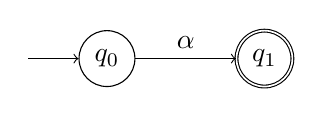
\begin{tikzpicture}
        \node[draw, circle] (A) at (0,0) {$q_0$};
        \draw[->] (-1,0) -- (A);
        \node[draw,circle,double] (B) at (2,0) {$q_1$};
        \draw[->] (A) -- (B);
        \draw (1,0) node [above] {$\alpha$};
     \end{tikzpicture}
     \rule{17cm}{0.5pt}\\
     \vspace{0.5cm}
     \caption{Automate reconnaissant $\alpha$ uniquement.}
     \label{fig:automate2}
 \end{figure}

 Nous allons maintenant prouver le sens réciproque. Pour cela, nous allons introduire une nouvelle classe d'automates, que l'on va appeler automates généralisés, dont les transitions seront étiquetées par des expressions rationnelles.

 \begin{defi}[Automate généralisé]
     Un automate généralisé est un automate dont la fonction de transition est définie par $\delta : \mathrm{Rat}(\Sigma)\times Q \to Q$ et qui ne possède qu'un état final. Un mot $u$ est accepté s'il peut être décomposé en $u_0\cdot u_1\cdots u_p$ et qu'il existe une suite $q_0,\ldots,q_{p+1}$ avec $q_{p+1}$ final et pour tout $i\leq p$, il existe $e\in\mathrm{Rat}(\Sigma)$ telle que $\delta(e,q_i)=q_{i+1}$ et $u_i\in L(e)$. De plus, on impose que $\delta$ n'est pas définie depuis $q_f$ l'état final et que $q_0$ n'est pas dans l'image de $\delta$.
 \end{defi}

 \begin{exo}
     Montrer que ces automates ont la même expressivité que les autres automates finis.
 \end{exo}

 \begin{rmk}
     Grâce à cet exercice, on peut supposer que pour tout automate $\aA$ il existe un automate généralisé $\aA'$ qui reconnaît le même langage.
 \end{rmk}

On va maintenant procéder sur l'automate généralisé en supprimant des transitions et des états jusqu'à n'obtenir qu'une seule transition, dont le label sera l'expression rationnelle associée à l'automate.

\begin{lem}[Réduction des transitions]
    Soit $\aA$ un automate généralisé, alors s'il existe $e,e'$ deux expressions et un état $q$ tels que $\delta(e,q)=\delta(e',q)$ alors on a un automate équivalent en supprimant ces deux transitions et en ajoutant $\delta(e+e',q)$.
\end{lem}

\begin{proof}
    Un mot reconnu par $\aA$ dont le chemin de lecture utilise $\delta(e,q)$ utilisera de la même façon $\delta(e+e',q)$, et réciproquement si un chemin de lecture utilise $\delta(e+e',q)$ alors soit le mot $u$ associé à cette transition est dans $L(e)$, auquel cas $\delta(e,q)$ donnera un chemin de lecture valide, soit il est dans $L(e')$ et $\delta(e',q)$ sera utilisé.
\end{proof}

On peut représenter cette réduction de la façon suivante :

\begin{figure}[htb]
    \centering
    \rule{17cm}{0.5pt}\\
    \vspace{0.5cm}
    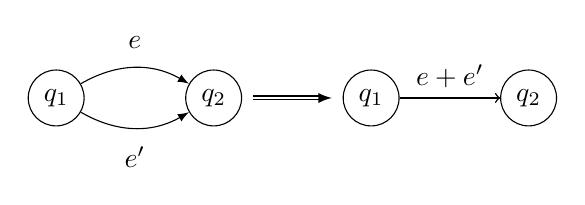
\begin{tikzpicture}
        \node[draw,circle] (A) at (-3,0) {$q_1$};
        \node[draw,circle] (B) at (-1,0) {$q_2$};
        \draw[->,>= latex] (A) to[bend left] (B);
        \draw[->,>= latex] (A) to [bend right] (B);
        \draw (-2,0.5) node [above] {$e$};
        \draw (-2,-0.5) node [below] {$e'$};
        \draw[->,>= latex, double distance = 1pt] (-0.5,0) -- (0.5,0);
        \node[draw,circle] (C) at (1,0) {$q_1$};
        \node[draw,circle] (D) at (3,0) {$q_2$};
        \draw[->,above] (C) -- (D);
        \draw[->,below] (C) -- (D);
        \draw (2,0) node [above] {$e+e'$};
    \end{tikzpicture}
    \rule{17cm}{0.5pt}\\
    \vspace{0.5cm}
    \caption{Réduction des transitions}
\end{figure}

Ainsi, par application successive du lemme, on peut supposer que l'on travail avec des états ne possédant qu'une transition entre deux états donnés. Nous allons maintenant procéder par élimination d'états.

\begin{lem}[\'Elimination des états]
    Soit un automate généralisé $\aA$ où l'on a réduit ses transitions, et $q$ un état ni initial ni final. Alors on peut construire un automate $\aA'$ reconnaissant le même langage en supprimant $q$ et, pour chaque couple d'états $(q_1,q_2)$ tel que $\delta(e_1,q_1)=q$ et $\delta(e_2,q)=q_2$, rajouter une transition de $q_1$ vers $q_2$ de la façon suivante :
    \begin{itemize}[label=$\bullet$]
        \item s'il existe $e$ telle que $\delta(e,q)=q$ alors on définit $\delta(e_1\cdot e^* \cdot e_2,q_1)=q_2$
        \item sinon, on définit $\delta(e_1\cdot e_2,q_1)=q_2$
    \end{itemize}
\end{lem}

\begin{proof}
    Dans le cas où le chemin de lecture ne passe pas par $q$, le lemme est évident. Supposons que dans la suite d'états $q_0,\ldots,q_p$ lisant un mot $u$ dans $\aA$ se trouve $q$, alors soit $q_1$ le prédécesseur de $q$ et $q_2$ son successeur (supposons d'abord que $q_2 \neq q$), dans la suite d'états. On sait qu'il existe une expression $e_1$ et une expression $e_2$ telles que $\delta(e_1,q_1)=q$ et $\delta(e_2,q)=q_2$ avec $u_1,u_2$ des parties du mot $u$ tels que $u_i\in L(e_i)$. Par définition, $u_1\cdot u_2\in L(e_1\cdot e_2)$ donc la suite d'états sans $q$ est valide dans $\aA$. Si jamais $q_2=q$, alors on peut remplacer toutes les suites de $q$ contiguës en disant que la transition est étiquetée par $e^*$ avec $e$ l'expression étiquetant la transition de $q$ à $q$.

    La réciproque est laissée en exercice au lecteur.
\end{proof}

On peut voit l'élimination d'états de la façon suivante :

\begin{figure}[htb]
    \centering
    \rule{17cm}{0.5pt}\\
    \vspace{0.5cm}
    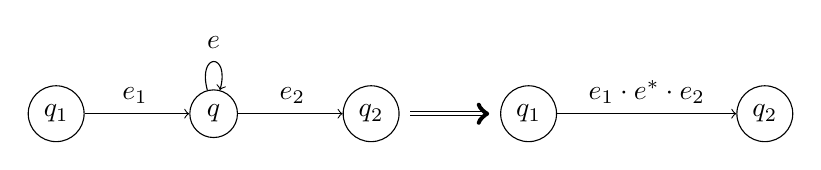
\begin{tikzpicture}
        \node[draw,circle] (A) at (-3,0) {$q$};
        \node[draw,circle] (B) at (-1,0) {$q_2$};
        \node[draw,circle] (E) at (-5,0) {$q_1$};
        \draw[->] (A) -- (B);
        \draw[->] (E) -- (A);
        \draw[->] (A) to[loop above] (A) ;
        \draw (-4,0) node [above] {$e_1$};
        \draw (-3,0.7) node [above] {$e$};
        \draw (-2,0) node [above] {$e_2$};
        \draw[->, double distance = 1pt] (-0.5,0) -- (0.5,0);
        \node[draw,circle] (C) at (1,0) {$q_1$};
        \node[draw,circle] (D) at (4,0) {$q_2$};
        \draw[->] (C) -- (D);
        \draw (2.5,0) node [above] {$e_1\cdot e^*\cdot e_2$};
    \end{tikzpicture}
    \rule{17cm}{0.5pt}\\
    \vspace{0.5cm}
    \caption{\'Elimination des états}
\end{figure}

On en déduit le résultat suivant :

\begin{prop}\label{prop:kleene2}
    Pour un automate généralisé $\aA$ il existe un automate généralisé $\aA'$ lisant le même langage et n'ayant qu'un état initial et un état final, et une seule transition entre les deux : le langage lu par $\aA'$ est exactement $L(e)$ pour $e$ l'étiquette de sa seule transition.
\end{prop}

\begin{proof}
    Il suffit de raisonner par récurrence sur le nombre d'états en appliquant l'élimination des états, et en réduisant les transitions qui en découlent. La dernière partie est par définition de la reconnaissance d'un mot dans un automate généralisé.
\end{proof}

On en déduit le théorème de Kleene :

\begin{them}[Kleene]
    La classe des langages rationnels est exactement l'ensemble des langages reconnus par des automates finis.
\end{them}

\begin{proof}
    C'est une conséquence directe des propositions \ref{prop:kleene1} et \ref{prop:kleene2}.
\end{proof}

\subsection{Myhill-Nérode}

Cette sous-section va s'attarder à une autre caractérisation des langages rationnels. Celle-ci est plus théorique mais présente plus facilement les limites des langages rationnels, et permet de répondre directement à la question \og y a-t-il pour un langage donné, un plus petit automate acceptant ce langage ?\fg{}

Tout d'abord, présentons un lemme en général utilisé pour montrer que des langages ne sont pas rationnels :

\begin{lem}[De l'étoile]
    Soit un langage rationnel $L$, alors il existe un nombre $M$ tel que pour tout mot $u\in L$ de longueur supérieure à $M$, il existe $v,w,x$ des mots ($w\neq\varepsilon$ mais les deux autres peuvent être vides) tels que $u = v\cdot w\cdot x$ et pour tout $n\in \nat$, $v\cdot w^n\cdot x \in L$. L'idée derrière est que pour les mots assez grands, il existe une partie du mot qui peut être répétée en restant dans le langage.
\end{lem}

\begin{proof}
    L'argument est principalement combinatoire : supposons que $u\in L$ avec $|u| > |Q|$ pour $Q$ l'ensemble d'états d'un automate $\aA$ reconnaissant $L$, alors lors de la lecture de $u$, on a la suite $q_0,\ldots,q_{|u|-1}$ et par principe des tiroirs, on trouve $i< j < |u|$ tels que $q_i = q_j$. On décompose alors le mot $u$ avec la partie préfixe $v := u_{<i}$, la partie infixe $w := u_{i,\ldots,j-1}$ et la partie postfixe $x := u_{j,\ldots,|u|-1}$. Dans ce cas, la lecture du mot $v\cdot w^n\cdot x$ donnera une suite d'états $q_0,\ldots,q_i$ puis $n$ fois la suite d'états de $q_i$ à lui-même décrite par $w$, puis la suite d'états $q_j,\ldots,q_{|u|-1}$  qui est un état final par hypothèse.
\end{proof}

\begin{rmk}
    Ce lemme est utile pour un langage infini : pour un langage fini, la constante sera simplement supérieure au cardinal du langage. De plus, la constante $M$ de ce lemme semble dépendre de l'automate reconnaissant le langage $L$, ce qui n'est pas naturel : le théorème de cette sous-section nous donnera justement une constante $M$ optimale et dépendant directement de $L$.
\end{rmk}

\begin{exo}
    En utilisant le lemme de l'étoile, montrer que le langage $\{0^n1^n\mid n\in\nat\}$ n'est pas rationnel.
\end{exo}

La notion principale pour pouvoir analyser les langages rationnels est celle de séparation des mots. L'idée derrière est simple : prenons deux mots $u$ et $v$, on peut les étendre naturellement en leur ajoutant un mot $z$ par concaténation, donnant $u\cdot z$ et $v\cdot z$. Dans ce cas, peut-on avoir un mot $z$ qui mène, depuis $u$, à un mot de $L$, et depuis $v$ à un mot qui n'est pas dans $L$ ? Cette notion motive notre prochaine définition :

\begin{defi}[Résiduel d'un langage]
    Soit $x$ un mot, on dénote par $x^{-1}L$ l'ensemble $$x^{-1}L=\{u\in \Sigma^*\mid x\cdot u \in L\}$$ appelé le résiduel de $L$ par $x$.

    De façon équivalente, on peut définir la relation d'équivalence d'inséparabilité : $x\sim y$ lorsque pour tout mot $u\in \Sigma^*$, $x\cdot u \in L \iff y\cdot u \in L$. Les classes d'équivalence pour cette relation sont les résiduels.
\end{defi}

Plusieurs observations s'ensuivent :
\begin{itemize}[label=$\bullet$]
    \item $L=\varepsilon^{-1}L$
    \item pour tout automate sur un langage $L$ fixé on peut associer à chaque état $q$ un résiduel de $L$.
\end{itemize}

Ces observations permettent d'imaginer les résiduels de $L$ comme un automate, lorsque le nombre de ses résiduels est fini. Le théorème de Myhill-Nérode stipule justement que ce nombre de résiduels est fini si et seulement si $L$ est rationnel.

\begin{them}[Myhill-Nérode]
    Soit $L$ un langage, alors $L$ est rationnel si et seulement s'il n'existe qu'un nombre fini de résiduels de $L$.
\end{them}

\begin{proof}
    Avec les observations antérieures, en supposant qu'il n'existe qu'un nombre fini de résiduels, on construit l'automate $\aA$ suivant :
    \begin{itemize}[label=$\bullet$]
        \item $Q = \{x^{-1}L\mid x \in \Sigma^*\}$
        \item $q_0 = \varepsilon^{-1}L$
        \item $\delta(\alpha,x^{-1}L) = (x\cdot \alpha)^{-1}L$ (la fonction est bien définie car si $x\sim y$ alors $x\cdot\alpha \sim y\dot\alpha$)
        \item $x^{-1}L$ est final s'il contient $\varepsilon$.
    \end{itemize}

    Si $x\in L$, alors $x^{-1}L$ contient $\varepsilon$ par construction, et s'il existe une suite d'états $q_0,\ldots,q_p$ menant à un état final dans cet automate, alors le dernier état est de la forme $x^{-1}L$ pour $x$ le mot lu et $\varepsilon\in x^{-1}L$ donc $x\cdot\varepsilon\in L$, c'est-à-dire $x\in L$. $L$ est donc reconnu par cet automate.

    Supposons que $L$ est rationnel. Alors soit $\aA$ un automate reconnaissant $L$. Pour chaque état $q$, on peut définir l'ensemble des mots menant de $q_0$ à $q$ : notons-le $P_q$. Alors pour deux mots $u,v\in P_q$, si $u\cdot z \in L$ alors $v\cdot z \in L$ car la lecture en partant de $q$ et en lisant les lettres de $z$ mène à un état final. Donc pour chaque état $q$, $P_q\subseteq x^{-1}L$ pour un certain $x$ (dépendant de $q$). On en déduit qu'il y a plus d'états que de résiduels, et comme l'automate est fini, qu'il y a un nombre fini de résiduels.
\end{proof}

\begin{rmk}
    La construction avec les résiduels nous donne donc aussi un automate minimal au sens du cardinal pour reconnaître un langage donné. Ainsi le lemme de l'étoile peut se reformuler en remplaçant \og il existe $M$\fg{} en remplaçant directement $M$ par le nombre de résiduels de $L$.
\end{rmk}

\begin{exo}
    Redémontrer que le langage $\{0^n1^n\mid n\in\nat\}$ n'est pas rationnel, cette fois-ci en utilisant le théorème de Myhill-Nérode.
\end{exo}

\begin{exo}
    L'ensemble des langages rationnels est-il stable par complémentaire ? Par intersection ?
\end{exo}

\begin{exo}
    Le langage des codes binaires de nombres multiples de $6$ est-il rationnel ?
\end{exo}

\begin{exo}
    Si $L$ est un langage rationnel, est-ce que le langage $\overline L$ des mots de $L$ à l'envers est rationnel ? Le langage des palindromes (mots qui sont les mêmes à l'envers) est-il rationnel ?
\end{exo}

La théorie des automates finis est bien plus vaste que le survol proposé ici : on peut par exemple parler de l'extension de ces automates aux mots infinis avec les automates de Büchi, ou encore de la détermination de l'arithmétique de Presburger avec des automates (ce dernier sujet aurait tout à fait sa place dans cet ouvrage dédié à la logique, mais comme l'objectif de ce chapitre n'est pas de voir en détail les automates mais seulement de mener naturellement aux machines de Turing, nous en ferons l'impasse).

Cependant, le problème avec les automates reste toujours le même : leur absence de mémoire et leur traitement purement linéaire de l'information. Le contre-exemple classique nous le montre bien : on ne peut pas compter de façon arbitrairement grande une valeur.


\subsection{Automates à pile}

Pour palier l'absence de mémoire de nos automates finis, l'idée naturelle est d'ajouter de la mémoire (jusque là, la solution paraît évidente). Il existe de nombreuses structures de données permettant de jouer la mémoire, mais comme l'indique le nom de nos automates, nous allons stocker les informations dans une pile, c'est-à-dire une structure linéaire de type \textit{last in first out}, où l'information extraite est la dernière information qui a été mise dans la pile. Le formalisme que nous utiliserons pour la pile est directement celui des mots : on peut représenter une pile par un mot $u$ sur lequel on ajoute ou enlève une lettre à gauche.

\begin{defi}[Automate à pile]
    Un automate à pile $\aA$ (non déterministe) est la donnée d'un tuple $(\Sigma,\Gamma,Q,q_0,\delta,F,\bot)$ où :
    \begin{itemize}[label=$\bullet$]
        \item $\Sigma$ est l'alphabet de lecture : c'est des mots de $\Sigma$ que l'on va reconnaître.
        \item $\Gamma$ est l'alphabet de pile : c'est avec cet alphabet que l'on écrira le mot qui nous servira de mémoire.
        \item $Q$ est l'ensemble des états.
        \item $q_0\in Q$ est toujours l'état initial.
        \item la fonction de transition est désormais $\delta : \Sigma^+\times \Gamma\times Q \to \mathcal P(\Gamma^*\times Q)$ où $A^+ = A \cup \{\varepsilon\}$
        \item $F\subseteq Q$ est l'ensemble des états finaux.
        \item $\bot\in \Gamma$ est le symbole de fond de pile : il indique que la pile est vide lorsqu'il est lu.
    \end{itemize}

    On appelle configuration interne une paire $(q,\gamma)\in Q \times \Gamma^*$ : cela représente l'état de l'automate à un instant donné. Une configuration est définie comme un triplet $(q,\gamma,u)\in Q\times \Gamma^*\times \Sigma^*$. On appelle transition entre deux configurations $(q,\alpha\cdot\gamma,\beta\cdot u)$ et $(q',\gamma'\cdot\gamma,u)$ la relation $(\gamma',q')\in\delta(\beta,\alpha,q)$, et on la note $(q,\alpha\cdot\gamma,\beta\cdot u) \vdash (q',\gamma'\cdot\gamma,u)$.

    On dit que le mot $u$ est accepté par $\aA$ s'il existe une suite de transitions depuis la configuration $(q_0,\bot,u)$ vers une configuration de la forme $(q_f,\gamma,\varepsilon)$ avec $q_f\in F$.
\end{defi}

Cette définition d'automate permet de définir la classe des langages algébriques, qui est une classe strictement plus large que les langages rationnels (elle contient par exemple le langage $\{0^n1^n\mid n\in\nat\}$)

Ceux-ci possèdent des propriétés de clôture différentes : ils sont clos par union, concaténation, et passage à l'étoile, mais aussi par passage au miroir. Enfin, l'intersection d'un langage rationnel et d'un langage algébrique est un langage algébrique.

Il existe une théorie parallèle, celle des grammaires, qui permet de donner une autre description équivalente des langages algébriques, mais nous ne nous attarderons pas dessus, car l'exemple des automates à pile nous sert surtout à introduire la notion de mémoire et de configuration. Remarquons simplement que la pile est un format de mémoire très limité : on peut y stocker des informations mais n'accéder qu'à une information à la fois. Nous allons donc voir un système plus expressif, avec une mémoire plus manipulable : les machines de Turing.

\section{Les machines de Turing}

L'idée des machines de Turing est assez similaire à celle d'automate à pile : simplement, au lieu d'utiliser une pile, nous utiliserons un ruban de mémoire, qui est une succession infinie de case, chacune contenant une lettre. La machine, au lieu de simplement prendre la lettre en haut de la pile, peut se déplacer librement sur le ruban pour lire et écrire sur le ruban de mémoire. Cette section sera dédiée à la présentation des machines de Turing, mais comportera peu de preuves : celles-ci, à cause du formmalisme lourd d'un système si complexe, sont trop techniques pour être présentées dans ce cours. Certaines idées de preuves seront données, tout de même.

\subsection{Des définitions équivalentes}

\begin{defi}[Machine de Turing]
    Une machine de Turing sur un alphabet $\Sigma$ est un tuple $(Q,\Gamma,q_0,\delta,q_a,q_r)$ où :
    \begin{itemize}[label=$\bullet$]
        \item $Q$ est l'ensemble des états de la machine.
        \item $\Gamma$ est l'alphabet de travail : c'est l'alphabet dans lequel seront les lettres du ruban de travail. On impose que $\Sigma\subseteq \Gamma$ et que $B\in\Gamma$ où $B$ est un symbole particulier, appelé symbole blanc, représentant l'absence d'écriture sur une case. On ajoute aussi le symbole $\rhd$ qui sera en début de ruban pour marquer qu'on est au début.
        \item $q_0$ est l'état initial de la machine.
        \item $\delta : Q\times \Gamma\to Q\times \Gamma \times \{\leftarrow,\rightarrow\}$ est la fonction de transition : elle considère l'état de la machine, la lettre lue et réécrit sur la case une nouvelle lettre, change d'état et fait bouger la tête de lecture vers la gauche ou la droite d'une case.
        \item $q_a\in Q$ est l'état acceptant : si la machine arrive dans cet état, le calcul s'arrête et le mot est accepté.
        \item $q_r\in Q$ est l'état de rejet : si la machine arrive dans cet état, le calcul s'arrête et le mot est rejeté.
    \end{itemize}
\end{defi}

Ces définitions ont peu de sens si l'on ne donne pas la définition de configuration et de ruban :

\begin{defi}[Ruban, configuration, transition]
    Le ruban de travail est un mot infini $r\in \Gamma^\omega$ sur l'alphabet de travail. On appelle configuration un tuple $(q,i,r)$ où $q$ est l'état de la machine de Turing, $r$ est le ruban et $i$ est l'indice de la case sur laquelle se trouve la tête de lecture. Plutôt que de noter cela comme un tuple, on note en général une configuration par un mot de la forme $r_{<i}qr_{\geq i}$, c'est-à-dire que l'on écrit les symboles qui sont à gauche de la tête de lecture, puis l'état dans lequel est la machine, puis le reste du mot. La tête de lecture se trouve donc sur la lettre juste à droite de l'état $q$ dans cette représentation.

    On appelle transition la fonction entre configurations définie de façon naturelle par la fonction de transition, en partant de la configuration $u\alpha q\beta r$ :
    \begin{itemize}
        \item si $\delta(q,\beta) = (q',a,\leftarrow)$ alors la transition sera $u\alpha q\beta r \to uq'\alpha a r$
        \item si $\delta(q,\beta) = (q',a,\rightarrow)$ alors la transition sera $u\alpha q\beta r \to u\alpha a q r$
    \end{itemize}

    On appelle calcul la suite de transitions depuis une configuration donnée (comme la machine est déterministe, la suite est unique, potentiellement infinie).
\end{defi}

De plus, on note $B^\infty$ la fin du ruban (remplie forcément de $B$ à l'infini).

\begin{defi}[Acceptation, rejet]
    Soit $x$ un mot sur un alphabet $\Sigma$ et $\MM$ une machine de Turing sur $\Sigma$. On dit que $\MM$ accepte $x$ si le calcul sur la configuration $q_0\rhd x B^\infty$ finit par $\MM$ entrant dans l'état $q_a$. On dit que $\MM$ rejette $x$ si le calcul sur la même configuration finit par $\MM$ entrant dans l'état $q_r$.
\end{defi}

\begin{rmk}
    Un mot $x$ peut n'être ni accepté, ni rejeté.
\end{rmk}

Donnons un exemple imagé d'une machine $\MM$ agissant sur la configuration $\rhd 0q1B^\infty$ en supposant que $\delta(q,1)=(0,q',\leftarrow)$ :

\begin{figure}[htb]
    \centering
    \rule{17cm}{0.5pt}\\
    \vspace{0.5cm}
    \begin{tikzpicture}
        \draw (-5,1) -- (5,1) -- (5,-1) -- (-5,-1) -- (-5,1);
        \draw (-3,1) -- (-3,-1);
        \draw (-1,1) -- (-1,-1);
        \draw (1,1) -- (1,-1);
        \draw (3,1) -- (3,-1);
        \draw[dashed] (5,1) -- (5.5,1);
        \draw[dashed] (5,-1) -- (5.5,-1);
        \draw (-4,0) node {\Huge $\rhd$};
        \draw (-2,0) node {\Huge $0$};
        \draw (0,0) node {\Huge $1$};
        \draw (2,0) node {\Huge $B$};
        \draw (4,0) node {\Huge $B$};
        \draw[<-] (0,-1) -- (0,-2);
        \draw (0,-1.5) node [right] {\Large $q$};

        \draw (-2,-2) -- (2,-2) -- (2,-4) -- (-2,-4) -- (-2,-2);
        \draw (0,-3) node {\Huge $\MM$};
        \draw[<-] (-2,-5) -- (-2,-4.5) -- (0,-4.5) -- (0,-4);
        \draw (0,-4.5) node [right] {\Large $q'$};
        
        \draw (-5,-5) -- (5,-5) -- (5,-7) -- (-5,-7) -- (-5,-5);
        \draw (-3,-5) -- (-3,-7);
        \draw (-1,-5) -- (-1,-7);
        \draw (1,-5) -- (1,-7);
        \draw (3,-5) -- (3,-7);
        \draw[dashed] (5,-5) -- (5.5,-5);
        \draw[dashed] (5,-7) -- (5.5,-7);
        \draw (-4,-6) node {\Huge $\rhd$};
        \draw (-2,-6) node {\Huge $0$};
        \draw (0,-6) node {\Huge $0$};
        \draw (2,-6) node {\Huge $B$};
        \draw (4,-6) node {\Huge $B$};
    \end{tikzpicture}
    \rule{17cm}{0.5pt}\\
    \vspace{0.5cm}
    \caption{Illustration de l'exécution d'une machine de Turing}
\end{figure}

Plusieurs versions équivalentes des machines de Turing existent, nous allons donner une liste et une façon de les simuler avec une machine à un ruban telle que décrite ici :
\begin{itemize}[label=$\bullet$]
    \item La machine peut se retrouver sur un ruban infini des deux côtés. Dans ce cas, comme on a une bijection entre $\nat$ et $\mathbb Z$ qui envoie $-n$ sur $2n+1$ et $n$ sur $2n$, il nous suffit de créer des états qui permettent de gérer des transitions de deux cases à chaque fois qu'il faut faire une transition d'une case, sauf sur la case d'indice $0$ où un changement d'état indiquera comment se comporter.
    \item On peut changer l'alphabet, et coder par exemple n'importe quel alphabet fini $\Sigma$ avec $\{0,1\}$ en considérant les cases par paquets (suffisamment gros pour pouvoir coder chaque élément de $\Sigma$ par un nombre binaire), ce qui augmentera largement le nombre d'états mais fonctionne. C'est d'ailleurs ce qu'il se passe dans les ordinateurs, où l'on code les données par paquets de $32$ ou $64$ bits.
    \item On peut considérer plusieurs rubans, et chaque tête de lecture se déplacera indépendamment. On peut simuler cela sur un ruban en considérant un alphabet plus gros : chaque case consistera en le $n$-uplet de cases de la machine à plusieurs rubans. Il faut néanmoins gérer le fait de bouger dans des sens différents : on peut pour cela considérer un alphabet encore plus gros qui serait constitué de parties de l'ancien alphabet et permettrait de faire une machine non déterministe.
    \item Une machine non déterministe peut se simuler avec une machine déterministe : chaque fois que plusieurs transitions sont possibles, on effectue une transition, puis on \og backtrack\fg{} (fait la transition inverse) pour faire l'autre transition. On effectue cette démarche pour chaque suite de transitions possibles de longueur $k$ et par $k$ croissant.
\end{itemize}

En bref, notre modèle est très expressif, mais malheureusement très peu manipulable dans le sens où se donner une machine de Turing concrète est très fastidieux. Nous n'en donnerons d'ailleurs pas ici : nous n'en donnerons que des codes, c'est-à-dire des suites de symboles qui peuvent être traduites en une machine de Turing. Plus précisément, tout algorithme écrit en pseudo-code correspondra à une machine de Turing (on l'admet ici).

Enfin, on peut construire une version équivalente des machine de Turing où, au lieu d'avoir des états acceptant et rejetant, on a un simple état d'arrêt, et la machine retourne le mot écrit sur le ruban lorsqu'elle s'arrête (puisque le mot infini contient une infinité de $B$, il le mot retourné est bien un mot fini). On appelle ces fonctions $\Sigma^*\to \Sigma^*$ des fonctions partielles calculables. On dit qu'une fonction est calculable quand elle est totale calculable.

\subsection{Les principaux théorèmes}

Un premier théorème fondamental dans la théorie de la calculabilité est celui qu'il existe une machine universelle :

\begin{them}
    Il existe une machine de Turing dite universelle, $\mathcal U$ sur un alphabet $\Sigma$ telle que, pour toute machine de Turing $\MM$ codée dans $\Sigma$ (le codage $\encode{\;}$ dépend de $\mathcal U$) et toute entrée $x$ codée dans $\Sigma$, $\mathcal U$ accepte $\langle \encode M,x\rangle$ si et seulement si $M$ accepte $x$, et refuse $\langle \encode M,x\rangle$ si et seulement si $M$ refuse $x$.
\end{them}

Comme dit plus tôt, nous ne donnerons pas de preuves pour ce genre de théorèmes, nous nous convaincrons seulement que l'on arrive en effet à coder un interpréteur pour un langage informatique donné, ce qui est l'analogue informatique d'une machine de Turing universelle.

La notation $\langle x,y\rangle$ sert à parler du codage d'un couple. Un codage simple dans l'alphabet $\{0,1\}$ est $1^{|x|}0 x y$ : l'information nous est donnée en comptant le nombre de $1$ de quelle taille fait $x$.

Le théorème suivant dit qu'on peut exécuter une machine sur elle-même :

\begin{them}[Récursion de Kleene]
    Soit $t$ une fonction calculable, il existe alors une machine de Turing $F$ telle que $t\encode F$ est une machine équivalente à $F$.

    Une version équivalente est qu'une machine $\MM$ a accès à son code source $\encode\MM$.
\end{them}

\subsection{Langage récursif, récursivement énumérable}

Naturellement, nous pouvons associer à une machine $\MM$ le langage $L(\MM)$ des mots reconnus par $\MM$. Cependant, on peut remarquer une différence importante : là où dans les anciens automates la lecture était linéaire et donc terminait forcément, ici nous n'avons aucune garantie que l'exécution d'une entrée $x$ sur $\MM$ va arriver à un état acceptant ou refusant. Ceci signifie qu'il existe deux classes de langages bien différentes :
\begin{itemize}[label=$\bullet$]
    \item les langages dits décidables, ou récursifs, qui sont ceux de la forme $L(\MM)$ pour une machine de Turing donnée qui, sur toute entrée, termine (i.e. tout calcul sur une entrée $x$ mène à un des deux états $q_a$ ou $q_r$).
    \item les langages dits récursivement énumérables, qui sont ceux de la forme $L(\MM)$ pour une machine de Turing $\MM$ (qui peut donc ne pas terminer).
\end{itemize}

De même, on différencie comme on l'a dit plus tôt les fonctions calculables des fonctions calculables partielles. Pour montrer l'importance de cette distinction, nous allons montrer qu'il existe des langages récursivement énumérables non récursifs.

\begin{rmk}
    Le nom de \og récursivement énumérable\fg{} vient du fait qu'une condition équivalente est qu'il existe une machine $\MM$ donnant la liste de tous les éléments du langage : une machine qui les énumère, donc. (\'Evidemment, ça ne suffit pas à décider si une entrée $x$ est dans le langage, puisqu'il faudrait avoir accèd à l'entièreté de la liste, en général infinie.)
\end{rmk}

\begin{defi}[Problème de l'arrêt]
    Soit $\mathrm{HALT} = \{\langle \encode \MM,x\rangle\mid \MM \text{ s'arrête sur l'entrée } x\}$. HALT est récursivement énumérable mais pas récursif.
\end{defi}

\begin{proof}
    L'existence d'une machine de Turing universelle suffit à montrer que le langage est récursivement énumérable : on exécute $\MM$ sur $x$ avec une machine universelle, et si elle termine on entre dans l'état acceptant. Maintenant, supposons que HALT soit récursif. On a donc une machine $\MM$ qui peut dit si une machine s'arrête sur une entrée donnée. On définit alors le programme $f$ suivant, prenant en entrée $x$ :
    \begin{itemize}[label=$\bullet$]
        \item si $\langle \encode x,x\rangle\in\mathrm{HALT}$ alors on crée une boucle infinie.
        \item sinon, on entre dans l'état $q_a$.
    \end{itemize}
    On remarque alors que, d'après le théorème de Kleene, on peut exécuter le programme $f$ en prenant son code en entrée : alors si $\langle \encode f,f\rangle \in\mathrm{HALT}$ on en déduit que $f(f)$ entre dans une boucle infinie, donc $\langle \encode f,f\rangle \notin\mathrm{HALT}$ et de même si $\langle \encode f,f\rangle\notin\mathrm{HALT}$ on en déduit que $\langle\encode f,f\rangle\in\mathrm{HALT}$.
\end{proof}

Un problème dont on sait qu'il n'est pas récursif est dit indécidable : c'est le cas du problème de l'arrêt, mais plus généralement d'une très large classe de langages. En effet, le prochain théorème montre que tout langage défini par une propriété non triviale (c'est-à-dire autre que toujours vraie ou toujours fausse) sur un langage récursivement énumérable est indécidable. On appelle une telle propriété une propriété sémantique : elle porte sur un langage récursivement énumérable, par contraste avec une propriété syntaxique qui porte sur les machines elles-mêmes (on peut par exemple compter le nombre de boucle \textit{While} d'un programme : les propriétés syntaxiques décrivent souvent des ensembles récursifs.

\begin{them}[Rice]
    Soit RE la classe des langages récursivement énumérables sur un alphabet $\Sigma$. Soit une partie $E$ de RE (donc une classe de langage), et $P$ l'ensemble des machines qui reconnaissent un ensemble $A\in E$ (donc les machines $\MM$ telles que $L(\MM)\in E$). $P$ est récursif si et seulement si $E=\varnothing$ ou $E=\mathrm{RE}$. 
\end{them}

\begin{exo}
    Montrer ce théorème en montrant que si $P$ est non trivial alors il peut se réduire au problème de l'arrêt, c'est-à-dire construire à partir d'un $P$ fixé une entrée du problème de l'arrêt, que l'on sait indécidable.
\end{exo}

\subsection{Fonctions récursives}

Le formalisme des machines de Turing permet d'avoir une approche qui fait un lien fort avec l'informatique, puisqu'il est le formalisme à la base même des ordinateurs et de la notion de programme et de code. Cependant, pour l'étude logique, un autre formalisme équivalent va être privilégié : celui des fonctions récursives. Nous allons donc voir les fonctions récursives, d'abord par les fonctions récursives primitives, et nous verrons ensuite l'équivalence entre fonction récursive et fonction calculable par une machine de Turing.

\subsubsection{Fonctions récursives primitives}

\begin{defi}[Classe RP]
On définit la classe des fonctions récursives primitives RP comme le plus petit sous-ensemble de fonctions $\nat^k\to\nat$, $k$ parcourant $\nat$, tel que :
\begin{itemize}[label=$\bullet$]
    \item pour chaque $n\in\nat$ et $k\in\nat$, la fonction $n : \nat^k\to\nat, x \mapsto n$ est dans RP.
    \item $S : \nat \to \nat, x \mapsto x+1$ est dans RP.
    \item les fonctions $\pi_i^k : \nat^k\to\nat, (x_1,\ldots,x_k)\mapsto x_i$ sont dans RP.
    \item si $f_1,\ldots,f_k : \nat^n \to \nat$ sont des fonctions de RP et $h : \nat^k\to\nat$, alors la fonction $h\langle f_1,\ldots,f_k\rangle : \nat^n \to\nat, x \mapsto h(f_1(x),\ldots,f_k(x))$ est aussi dans RP.
    \item si $f : \nat^k\to\nat$ et $g : \nat^{k+2}\to\nat$ sont des fonctions de RP, alors la fonction $\rec(f,g) : \nat^{k+1} \to\nat$ est dans RP, où \begin{align*}
        \rec(f,g)(x,0) &= f(x)\\
        \rec(f,g)(x,S(n)) &= g(x,n,\rec(f,g)(x,n))
    \end{align*}
\end{itemize}
\end{defi}

Le point important pour l'expressivité de cette classe de fonction est évidemment le fait d'autoriser les appels récursifs. On peut construire de nombreuses fonctions usuelles par cette classe.

\begin{exo}
    Montrer que les fonctions suivantes sont dans RP :
    \begin{itemize}[label=$\bullet$]
        \item La fonction identité $x \mapsto x$
        \item La fonction somme : $\nat^2\to\nat, (x,y)\mapsto x+y$
        \item La fonction produit : $\nat^2\to\nat, (x,y)\mapsto x\times y$
        \item La fonction puissance : $\nat^2\to\nat, (x,y)\mapsto x^y$
        \item La fonction prédécesseur : $\nat\to\nat, x \mapsto \max(0,x-1)$
        \item La fonction différence : $\nat^2\to\nat, (x,y)\mapsto \max(0,x-y)$
        \item La fonction moitié : $\nat\to\nat,x \mapsto \lfloor x/2\rfloor$
        \item La fonction division : $\nat^2\to\nat, (x,y)\mapsto \lfloor x/y\rfloor$ et $0$ si $y=0$
        \item La fonction reste : $\nat^2\to\nat, (x,y)\mapsto x\%y$ le reste de $x$ par la division par $y$, et $0$ si $y=0$
        \item Pour tout polynôme de $\nat[X]$, la fonction $\nat\to\nat$ associée.
        \item Pour $f,g,h$ trois fonctions de RP, la fonction $\texttt{if}(f,g,h) : x \mapsto g(x)$ si $f(x)=0$ et $h(x)$ sinon.
    \end{itemize}
\end{exo}

\begin{exo}\label{exo:bij}
    Montrer que la fonction $b : \nat^2\to\nat, (x,y)\mapsto \frac{1}{2}(x+y)(1+x+y)+y$ établit une bijection entre $\nat^2$ et $\nat$. Construire aussi les fonction $\pi_1$ et $\pi_2$ telles que $\pi_1(b(x,y))=x$ et $\pi_2(b(x,y))=y$.
\end{exo}

On peut aussi analyser des ensembles grâce à leur fonction caractéristique.

\begin{exo}
    Construire les fonctions caractéristiques des ensembles suivants :
    \begin{itemize}[label=$\bullet$]
        \item $\nat_{>k}$ pour $k\in\nat$
        \item $\{0\}$
        \item $n\nat$
        \item $\{(x,x)\mid x\in\nat\}$
        \item $\{(x,y)\mid x < y\}$
        \item $\{(x,y)\mid y=P(x)\}$ où $P\in\nat[X]$ est fixé.
    \end{itemize}
\end{exo}

\subsubsection{Opérateur mu}

Cependant, toutes les fonctions calculables par des machines de Turing ne sont pas forcément dans RP : certaines croissent trop vite. En effet, une remarque assez directe est que les fonctions récursives primitives ne peuvent pas appliquer une fonction un nombre non borné de fois : il faut calculer au préalable une borne supérieure du nombre d'application de notre fonction. De plus, toutes les fonctions dans RP sont des fonctions totales, alors que nous voulons pouvoir écrire des fonctions partielles. Nous allons donc définir Rec, la classe des fonctions récursives, en ajoutant un constructeur :

\begin{defi}[Classe Rec]
    La classe Rec est la classe RP à laquelle on ajoute le constructeur $\mu$ : si $f : \nat^{k+1}\to\nat$ est dans Rec, alors $g(x_1,\ldots,x_k)=\mu(y,f)$ renvoie le plus petit $y$ tel que $f(x_1,\ldots,x_k,y) = 0$ et pour tout $x<y$, $f(x_1,\ldots,x_k,x)$ est définie, et n'est pas définie sinon.
\end{defi}

Il se trouve que Rec est exactement la classe des fonctions calculables partielles.

\begin{them}[Simulation des machines de Turing]
    Soit $\MM$ une machine de Turing sur $\{0,1\}$ définissant une fonction $f : \nat \to \nat$ à partir de son comportement sur $\{0,1\}^*\to\{0,1\}^*$. Alors $f\in\mathrm{Rec}$.
\end{them}

\begin{proof}
    Nous allons pour cela construire par étape une fonction $f$ récursive qui simule $\MM$ :
    \begin{itemize}[label=$\bullet$]
        \item Nous allons coder les états de $\MM$ par des entiers.
        \item Une configuration peut être vue comme un élément de $\nat^3$ avec ce codage : nous allons donc construire une fonction qui effectue une transition, ou plus précisément trois fonctions, l'une retournant le nouvel indice de la tête de lecture, la deuxième retournant le code de l'état et la troisième retournant la forme nouvelle du ruban.
        \item Cette fonction peut se faire par disjonction de cas : on sait coder la fonction caractéristique de chaque entier, et faire des branchements if/then/else. Il ne reste qu'à effectuer cette disjonction de cas sur chaque état en entrée, puis une disjonction de cas suivant si le symbole lu est $0$ ou $1$. La fonction d'indice décrémente ou incrémente l'indice directement, ce que l'on peut faire, la fonction d'état associe une constante, et la fonction de ruban n'a qu'à effectuer de l'arithmétique pour ajouter ou soustraire $2^i$ avec $i$ l'indice de la tête de lecture.
        \item Si l'on nomme $g$ cette fonction, on peut alors l'appliquer en boucle jusqu'à obtenir un résultat. C'est ici que l'on a besoin de $\mu$, qui s'appliquera à la fonction caractéristique de l'état d'arrêt composée avec la fonction qui pour $i$ effectue $i$ itérations de $g$.
    \end{itemize}
\end{proof}

\begin{rmk}
    La construction d'une fonction récursive simulant une machine de Turing ne nécessite l'opérateur $\mu$ que pour pouvoir appliquer l'opération de transition un nombre non borné de fois : cela signifie que pour une machine $\MM$ où l'on peut borner son temps de calcul en fonction de son entrée, il suffit d'une fonction primitive récursive pour coder la machine $\MM$.
\end{rmk}


\chapter{Arithmétique de Peano et incomplétude}

Nous avons étudié la logique des prédicats, mais ne l'avons pas encore mise en \oe uvre. Ce chapitre en sera une première application : nous allons introduire l'axiomatisation de l'arithmétique de Peano, c'est-à-dire la théorie axiomatique définissant les entiers naturels usuellement. Nous commencerons donc par énoncer les axiomes de la théorie nommée PA, pour ensuite définir quelques propriétés basiques. Historiquement, l'axiomatisation de l'arithmétique a été la première réussite du logicisme : réussir à formuler de façon purement formelle ce que nous entendons par les entiers et leurs relations usuelles. C'est cette réussite qui a mené David Hilbert à poser la question à toute la communauté scientifique : \og arriverons-nous à décider toute proposition arithmétique de façon purement mécanique ?\fg{} (Nous dirions maintenant \og existe-t-il un algorithme décidant les proposition vraies ?\fg{} mais le problème a été posé avant que la théorie de la calculabilité émerge). La réponse, bien connue maintenant, est non : non seulement il n'existe pas d'algorithme permettant de décider les propositions, mais tout système suffisamment expressif pour parler de toute l'arithmétique, mais suffisamment restreint pour être manipulable, possède des propositions qui sont indécidables, c'est le premier théorème d'incomplétude de Gödel. Nous reviendrons à la fin du chapitre sur ce théorème, ainsi que le second, qui sont des passages obligés du traitement moderne de la logique. Bien sûr, nous avons maintenant l'outil de la calculabilité qui rendra beaucoup plus digeste (bien que toujours très dur à assimiler) la preuve que nous ferons du premier théorème, là où historiquement la preuve est plus vieille que la notion de machine de Turing. Le second théorème d'incomplétude sera mentionné mais non développé, pour des raisons que nous développerons dans la dernière section.

\section{Axiomes de Peano}

Nous allons donc expliciter la théorie axiomatique PA. Pour cela, donnons d'abord le langage de l'arithmétique : $\LL=\{0,S,+,\times\}$ où, sans surprise, $0$ est une constante, $S$ une fonction d'arité $1$ représentant la fonction $x\mapsto x+1$, $+$ et $\times$ des fonctions d'arité $2$. On pourrait ajouter $\leq$ une relation binaire, mais nous allons voir que nous pouvons la définir de façon peu coûteuse. L'idée de notre définition de $\nat$ est que $\nat$ est défini comme une structure inductive avec une constante et un constructeur unaire.

Plutôt que d'énoncer tous les axiomes de Peano à la suite, nous allons nous concentrer sur chacun d'eux (ou au moins chaque groupe). 

\begin{defi}[Axiomes du successeur]
    Le premier axiome est $A_1 := \forall x. \lnot (S x = 0)$, nous nous permettrons d'écrire $\lnot (a=b)$ par $a\neq b$.

    Le second axiome est $A_2 := \forall x. \exists y.(x\neq 0 \to S y = x)$.

    Le troisième axiome est $A_3 := \forall x.\forall y. ((S x = S y)\to (x=y))$
\end{defi}

Ces axiomes traduisent le comportement de l'opération $S$ : $0$ n'est le successeur de personne, mais tout autre élément est le successeur d'au moins un élément, et la fonction $S$ est injective (donc il n'existe finalement qu'un seul prédécesseur à un entier non nul). Les axiomes qui suivent définissent $+$ et $\times$ :

\begin{defi}[Axiomes de l'addition]
    Les deux axiomes suivants sont :
    \begin{align*}
        A_4 &:= \forall x. (x+0=x)\\
        A_5 &:= \forall x. \forall y. x + (S y) = S (x + y)
    \end{align*}
\end{defi}

Ces axiomes traduisent directement la définition récursive de l'addition. De même les deux axiomes suivants définissent la multiplication de façon récursive :

\begin{defi}[Axiomes de la multiplication]
    Les deux axiomes suivants sont :
    \begin{align*}
        A_6 &:= \forall x. (x\times 0 = 0)\\
        A_7 &:= \forall x.\forall y. x\times (S y) = (x\times y) + x
    \end{align*}
\end{defi}

On note alors $\PA_0$ la théorie $\PA_0 = \{A_1,A_2,A_3,A_4,A_5,A_6,A_7\}$. Cette théorie est très faible : elle ne permet aucune preuve par récurrence. Ceci est dû au fait qu'a priori, tous les éléments ne sont pas forcément des successeurs de $0$ : simplement qu'un élément est localement un successeur ou $0$. Cependant, si l'énoncé commun de la récurrence est \og toute partie $F\subseteq\nat$ contenant $0$ et stable pour $S$, càs telle que $x\in F \implies S x \in F$ alors $F=\nat$\fg{}, cette quantification sur les parties $F\subseteq\nat$ n'est pas définissable dans notre théorie du premier ordre (c'est exactement une quantification du second ordre). Cependant, de la façon dont on se sert de la récurrence, on remarque que la notion importante est celle de proposition, et non de sous-ensemble : on veut que toute proposition vraie pour $0$ et dont la vérité à un rang implique sa vérité au rang suivant est vraie pour tous les objets. Cette version peut se faire, pour une proposition donnée : il suffit d'écrire pour une proposition $P$ la proposition $P(0)\land (\forall x.P(x)\to P(S(x)))\to \forall x. P(x)$ et de l'ajouter en axiome. L'idée est donc, alors, d'ajouter autant d'axiomes que nous avons de propositions : on va définir alors ce qu'on appelle un schéma d'axiomes (c'est-à-dire un ensemble d'axiomes dont on décrit la forme, de façon équivalente dont on donne un algorithme de construction).

\begin{defi}[Schéma d'axiomes de récurrence]
    Pour $P$ une proposition à $n$ variables libres $x_0,\ldots,x_n$, la proposition $$\forall x_1.\ldots\forall x_n.((P(0,x_1,\ldots,x_n)\land \forall x.(P(x,x_1,\ldots,x_n)\to P(S(x),x_1,\ldots,x_n)))\to \forall x. P(x,x_1,\ldots x_n))$$ appartient à l'ensemble $\mathcal P_\mathrm i$.
\end{defi}

\begin{lem}[Récursivité de la récurrence]
    L'ensemble $\mathcal P_\mathrm i$ est un langage récursif (et donc décidable) sur $(\LL\cup\{(,),\lor,\land,\to,\lnot,\forall.,\exists.\})^*$.
\end{lem}

\begin{proof}
    Nous ne donnerons pas une réelle démonstration ici mais une idée de pourquoi le résultat est vraie (une démonstration rigoureuse nécessiterait d'entrer en détails dans le fonctionnement des machines de Turing, ce que nous nous refusons de faire pour garder une certaine lisibilité). Ce résultat vient directement du fait qu'on a donné une description algorithmique de $\mathcal P_\mathrm i$ (on pourrait penser que cela nous donne uniquement un ensemble récursivement énumérable, mais on peut par exemple ordonner les propositions par longueur et considérer le nombre de symboles de la proposition dont on veut savoir si elle est dans $\mathcal P_\mathrm i$ : il n'y aura qu'un nombre fini de propositions plus petites qu'il faudra donc tester).
\end{proof}

On peut alors définir PA comme l'ensemble précédent muni du schéma d'axiomes de récurrence.

\begin{defi}[Théorie PA]
    On définit $\PA := \PA_0 \cup \mathcal P_\mathrm i$.
\end{defi}

\begin{lem}[Récursivité de PA]
    PA est un langage récursif.
\end{lem}

\begin{proof}
    Il suffit de tester pour une proposition si elle est l'une des $7$ premières puis d'exécuter l'algorithme pour vérifier si la proposition est dans $\mathcal P_\mathrm i$.
\end{proof}

\begin{exo}
    Montrer que les axiomes de $\mathcal P_\mathrm i$ peuvent être remplacés par une nouvelle règle :
    \begin{center}
        \begin{prooftree}
            \hypo{\Gamma\vdash P(0)}
            \hypo{\Gamma\vdash \forall x. P(x)\to P(S(x))}
            \infer2[Rec]{\Gamma\vdash \forall x. P(x)}
        \end{prooftree}
    \end{center}
    et que l'on peut alors définir PA comme la théorie $\PA_0$ enrichie de cette règle logique dans la relation de dérivation de jugement logique. \textit{Remarque : Cette règle n'a de sens que dans le langage de l'arithmétique, et on présuppose largement que $\Gamma\subseteq\PA_0$ pour que la règle ait un sens.}
\end{exo}

\begin{exo}
    Montrer qu'il existe un modèle non standard de PA, c'est-à-dire un modèle qui n'est pas l'ensemble usuel des entiers naturels. \textit{Indication : on introduira une constante dont on montrera qu'elle n'est égale à aucun entier naturel en utilisant le théorème de compacité.}
\end{exo}

\section{L'arithmétique telle que nous la connaissons}

On peut alors commencer à prouver des résultats semblant évidents mais qui n'appartiennent pas directement à la théorie. Nous ne donnerons pas d'arbre de preuve mais seulement des arguments. Leur mise en arbre de preuve sera laissée en exercice.

\begin{prop}[Neutre]
    $0$ est neutre pour $+$, c'est-à-dire que \begin{align*}
        \forall x.x+0=x\\
        \forall x.0+x=x
    \end{align*}

    $1$ est neutre pour $\times$ :
    \begin{align*}
        \forall x. x\times 1=x\\
        \forall x. 1\times x=x
    \end{align*}
\end{prop}

\begin{proof}
    La première proposition est purement un axiome de notre théorie, mais la neutralité à gauche de $0$ est déjà à prouver (par récurrence évidemment). D'abord $0+0=0$ en appliquant l'axiome $A_4$, puis si $0+x=x$ alors $0+(S x) = S (0+x) = S x$ en remplaçant $0+x$ par $x$ grâce à l'hypothèse. Donc pour tout $x$, $0+x=x$.

    La neutralité à droite de $1$ pour $\times$ est un simple calcul :
    \begin{align*}
        x\times 1 &= x\times (S 0)\\
        &= (x\times 0) + x\\
        &= x
    \end{align*}
    pour la neutralité à gauche, nous allons encore raisonner par récurrence : d'abord $1\times 0 = 0$ grâce à l'axiome $A_6$, puis si l'on suppose que $1\times n = n$ alors $1\times (S n) = (1\times n) + 1$ puis on remarque que $n+1=S n$ de façon directe, eet que $1\times n = n$ par hypothèse de récurrence, nous donnant que $1\times (S n) = S n$.
\end{proof}

\begin{prop}[Associativité et commutativité de l'addition]
    L'addition est associative et commutative, ce qui signifie :
    \begin{align*}
        \forall x.\forall y.\forall z. x+(y+z) = (x+y)+z\\
        \forall x.\forall y. x+y = y+x
    \end{align*}
\end{prop}

\begin{proof}
    Prouvons le premier point par récurrence sur $z$ (quitte à échanger les variables) : dans le premier cas, on a $x+y=x+y$ après réduction des additions de $0$ à droite. Si l'on suppose que $x+(y+z)=(x+y)+z$ alors $x+(y+S z) = x+S(y+z)=S(x+(y+z))$ et ici, par hypothèse de récurrence, on peut remplacer $x+(y+z)$ par $(x+y)+z$ et on finit la chaîne d'égalités par $S((x+y)+z) = (x+y) + Sz$, prouvons la propriété par récurrence.

    Pour le deuxième point, nous prouverons un lemme intermédiaire : $\forall x.\forall y. S(x+y)=Sx+y$ par récurrence sur $y$ : dans le cas nul, on a $S(x+0) = S(x) + 0$ qui est vrai. Si $\forall x.S(x+y)=Sx+y$, alors $Sx+Sy = S(Sx+y)$ et par application de l'hypothèse de récurrence, en remplaçant $x$ par $Sx$, on en déduit que $S(Sx+y) = SS(x+y)$, et $SS(x+y) = S(x+Sy)$ donc $$Sx+Sy=S(x+Sy)$$ ce qui complète notre démonstration par récurrence.

    Montrons maintenant la commutativité par récurrence sur $y$ : dans le cas nul, on doit montrer que $x+0=0+x$ ce qui se fait grâce au fait que $0$ est neutre. Supposons que $\forall x. x+y=y+x$, alors en fixant un certain $x$, $x+Sy=S(x+y)$ puis par hypothèse de récurrence, $S(x+y)=S(y+x)$ et en utilisant le lemme précédent, $S(y+x)=Sy+x$, donc $$x+Sy=Sy+x$$ concluant notre preuve par récurrence.
\end{proof}

Nous allons maintenant prouver la distributivité.

\begin{prop}[Distributivité]
    La multiplication est distributive sur l'addition, c'est-à-dire que : $$\forall x.\forall y.\forall z.x\times(y+z) = x\times y + x\times z$$ en prenant les conventions de priorité habituelles, et $$\forall x.\forall y.\forall z. (x+y)\times z = x\times z + y\times z$$
\end{prop}

\begin{proof}
    Prouvons le premier résultat par récurrence sur $z$ : dans le cas où $z=0$, on trouve $\forall x.\forall y.x\times (y+0) = x\times y + x\times 0$, ce qui se vérifie facilement. Dans le cas où $\forall x.\forall y. x\times (y+z) = x\times y + x\times z$, alors pour $x,y$ fixéx, \begin{align*}    x\times (y+Sz)&=x\times S(y+z) \\
     &= (x\times (y+z)) + x \\
     &= (x\times y + x\times z) + x\\
     &= x\times y + (x\times z +z)\\
     &= x\times y + x \times (S z)
     \end{align*}
     ce qui conclut la récurrence.

     Le deuxième résultat se prouve aussi par récurrence sur $z$ : pour $z=0$, on trouve $\forall x.\forall y. (x+y)\times 0 = 0 =x\times 0 + y\times 0$. Si $\forall x.\forall y. (x+y)\times z=x\times z + y\times z$ alors \begin{align*}
         (x+y)\times Sz &= (x+y)\times z + (x+y)\\
         &= (x\times z + y\times z) + (x + y)\\
         &= (x\times z + x) + (y\times z + y)\\
         &= (x\times Sz) + (y\times Sz)
     \end{align*}
     ce qui conclut la récurrence.
\end{proof}

De même, démontrons ces propriétés pour la multiplication.

\begin{prop}[Associativité et commutativité de la multiplication]
    La multiplication est associative et commutative.
\end{prop}

\begin{proof}
    On raisonne encore par récurrence sur $z$ : dans le premier cas tout se simplifie en $0=0$. Si $\forall x.\forall y.x\times (y\times z)=(x\times y)\times z$, alors pour $x,y$ fixés, on a \begin{align*}
        x\times (y\times Sz) &= x\times (y \times z + y)\\
        &= x\times (y\times z) + x\times y\\
        &= (x\times y)\times z + x\times y\\
        &= (x\times y)\times Sz
    \end{align*}
    ce qui conclut la récurrence.

    Pour la commutativité le cas de $y=0$ est évident. Si l'on suppose que $\forall x.x\times y=y\times x$, alors pour prouver que $x\times Sy = Sy\times x$, nous allons procéder par récurrence sur $x$ : $0\times Sy = Sy\times 0$ de façon évidente, et si $x\times Sy = Sy\times x$, alors \begin{align*}
        Sy\times Sx &= (Sy\times x) + Sy\\
        &= (x\times Sy) + Sy\\
        &= ((x\times y) + x) + Sy\\
        &= (x\times y) + (x+Sy)\\
        &= (x\times y) + S(x+y)\\
        &= (x\times y) + S(y+x)\\
        &= (x\times y) + (y+Sx)\\
        &= ((x\times y) + y) + Sx\\
        &= ((y\times x) + y) + Sx\\
        &= (y\times Sx) + Sx\\
        &= (Sx \times y) + Sx\\
        &= Sx\times Sy
    \end{align*}
    donc on en déduit que $\forall x. x\times Sy=Sy\times x$, donc on en déduit que $\forall y.\forall x. x\times y = y\times x$.
\end{proof}

Les opérations sont aussi régulières :

\begin{prop}[Régularité]
    On a $$\forall x.\forall y.\forall z. (x+z = y+z) \implies x=y$$ \begin{center} et \end{center} $$\forall x.\forall y.\forall z. (z\neq 0) \implies (x\times z = y\times z)\implies x=y$$
\end{prop}

\begin{proof}
    Prouvons la proposition par récurrence sur $z$ : le premier cas est $x+0=y+0$ d'où $x=y$. Si $(x+z=y+z)\implies x=y$, alors supposons que $x+Sz=y+Sz$, par axiome on a $S(x+z)=S(y+z)$ puis, encore par axiome, que $x+z=y+z$ donc $x=y$.

    Prouvons la deuxième proposition par récurrence sur $x$ et $y$ (d'abord sur $x$ puis sur $y$). Pour $x=0$, on suppose que $x\times z = y\times z$ donc que $y\times z = 0$ et que $z\neq 0$, donc $y=0=x$. Supposons alors que pour tout $y,z$, $(z\neq 0) \implies (x\times z = y\times z) \implies x=y$, et prouvons que le résultat $\forall y.\forall z.(z\neq 0)\implies (S x \times z = y\times z) \implies x =y$ est vrai par récurrence sur $y$. Dans le cas nul, on retrouve le raisonnement précédent. On suppose donc maintenant que pour tout $z$, $(z\neq 0)\implies (S x\times z = y\times z) \implies x=y$ et on veut prouver que pour tout $z$, $(z\neq 0)\implies (S x \times z = S y \times z)\implies x =y$. Supposons donc que $S x \times z = S y \times z$, alors $z\times S x = z\times S y$ par commutativité, puis par définition $z\times x + z = z\times y + z$, d'où par régularité de l'addition, $z\times x = z\times y$. Alors puisque par hypothèse $z\neq 0$, on peut appliquer l'hypothèse d'induction du début pour déduire que $x=y$.
\end{proof}



Les opérations d'addition et de multiplication se comportent bien comme on l'attend, ce qui est très rassurant quant à notre axiomatisation (avec le principe de récurrence et $7$ axiomes, nous avons déjà de nombreuses propriétés qui semblent bien correspondre à celles de $(\nat,+,\times)$).

\section{Extension possible, fonction représentable}

Tout d'abord, on peut définir le prédicat $x\leq y$ en disant que ce symbole, à l'origine hors du langage, est juste une façon rapide d'écrire $\exists k. x + k = y$ : en effet être inférieur pour les entiers signifie simplement qu'il y a une différence positive entre les deux entiers. On peut alors montrer que $x\leq y$ est bien une relation d'ordre, et même qu'elle est totale.

\begin{exo}
    Montrer que $\leq$ est une relation d'ordre totale dans PA. Montrer de plus qu'elle est compatible avec l'addition, c'est-à-dire que $$\forall x.\forall y.\forall z. (x\leq y) \implies (x+z\leq y+z)$$ et avec la multiplication : $$\forall x.\forall y.\forall z. (x\leq y)\implies (x\times z \leq y \times z)$$
\end{exo}

Nous pouvons donc facilement définir des prédicats en tant que sucre syntaxique : un prédicat pouvant déjà se définir par une proposition, il nous suffit de travailler au sein des propositions. Cependant, si l'on veut définir une fonction $f$ au sein de la théorie, comment faire ? Pour cela, nous allons avoir besoin d'abord de déterminer ce que l'on appelle le modèle standard de PA, qui est $\nat$ dans son sens usuel.

\begin{defi}[Modèle standard de PA]
    On définit $\nat$, le modèle standard de PA, par les définitions suivantes :
    \begin{itemize}[label=$\bullet$]
        \item $|\nat|$ est l'ensemble des entiers naturels tels que l'on les entend en général (à la limite, penser à leur construction dans ZF, si l'on veut être formaliste, mais sinon il suffit de s'imaginer ce qu'on entend intuitivement par $\nat$ : l'ensemble des nombres finis)
        \item $0$ est interprété par l'entier $0$
        \item $S$ est interprété par la fonction $x\mapsto x+1$
        \item $+$ est interprété par l'addition évidente.
        \item $\times$ de même.
    \end{itemize}
    Remarquons que chaque $n$ de $\nat$ est exactement représenté par $S^n0$ où l'on considère l'application en boucle de $S$, $n$ fois. Nous noterons $\overline n$ pour considérer le représentant dans PA du nombre $n\in \nat$.
\end{defi}

\begin{exo}
    Montrer que tout modèle de PA possède un sous-modèle isomorphe à $\nat$, et que de plus il en est un segment initial, au sens où si $n$ est l'image d'un entier standard et $m\leq n$ alors $m$ est l'image d'un entier standard.
\end{exo}

En réalité, ce qui nous intéresse en premier lieu dans PA est de formaliser $\nat$ : si l'on peut prouver l'existence de modèles non standards de PA, l'important est que tout modèle non standard possède un représentant de $\nat$, et que l'on peut donc y définir des fonctions $\nat^k\to\nat$ par exemple.

Par exemple ? Non, c'est exactement le cadre des fonctions récursives, et ce que nous allons vouloir faire maintenant est de montrer que l'on peut représenter les fonctions récursives dans PA. Commençons par définir une fonction représentable en général.

\begin{defi}[Fonction représentable]
    Soit $f : \nat^k\to\nat$ une fonction (totale), on dit que $f$ est représentable dans PA lorsqu'il existe une formule $F$ à $k+1$ variables libres telle que pour tous entiers $n_1,\ldots,n_k$, on a $$\PA\vdash \forall y.(F(y,\overline{n_1},\ldots,\overline{n_k}) \leftrightarrow y = \overline{f(n_1,\ldots,n_k)})$$
\end{defi}

Une fonction représentable est donc une fonction dont on peut définir le fait d'appartenir à son graphe par une formule $F$. Remarquons que l'on ne définit pas une formule close ici : on veut pouvoir donner en entrée à notre formule $F$ les paramètres de notre fonction $f$.

Nous allons de même définir un ensemble représentable comme correspondant à une proposition :

\begin{defi}[Ensemble représentable]
    Un ensemble $A\subseteq \nat^k$ est dit représentable s'il existe une proposition $F$ à $k$ variables libres $x_1,\ldots,x_k$ telle que :
    \begin{itemize}[label=$\bullet$]
        \item si $(x_1,\ldots,x_k)\in A$ alors $\PA\vdash F(\overline{x_1},\ldots,\overline{x_k})$
        \item si $(x_1,\ldots,x_k)\notin A$ alors $\PA\vdash \lnot F(\overline{x_1},\ldots,\overline{x_k})$
    \end{itemize}
\end{defi}

\begin{exo}
    Montrer que $A$ est représentable si et seulement si sa fonction caractéristique $1_A$ est représentable.
\end{exo}

Montrons donc que les fonctions de base de RP sont représentables :

\begin{itemize}[label=$\bullet$]
    \item La fonction successeur est évidemment représentable par $S$.
    \item La projection $\pi_i^k$ est représentée par la formule à $k+1$ variables $x_0=x_i$ (en reprenant les conventions précédentes).
    \item La fonction constante est représentée par la formule à $k+1$ variables $x_0 = \overline k$.
\end{itemize}

Nous allons ensuite prouver la stabilité pour les trois schémas : la composition, la récursion et l'opérateur $\mu$. Rappelons d'après notre théorème de simulation des machines de Turing qu'une fonction récursive est une fonction récursive primitive à laquelle on n'a appliqué qu'une seule foie l'opération $\mu$.

\begin{lem}[Représentabilité de la composition]
    Si $f_1,\ldots,f_p : \nat^k \to \nat$ sont représentables et $g : \nat^p \to \nat$ est représentable, alors la fonction $f : \nat^k\to\nat, x \mapsto (f_1(x),\ldots,f_p(x))$ est représentable.
\end{lem}

\begin{proof}
    Soient $f_1,\ldots,f_p$ des fonctions représentables à $k$ entrées et $g$ une fonction représentable à $p$ entrée, représentées respectivement par $F_1,\ldots,F_p,G$. On va représenter $f$ par la proposition $$F(x_0,\ldots,x_k) := \exists y_1.\ldots \exists y_p. (G(x_0,y_1,\ldots,y_p)\land \bigwedge_{1\leq i \leq n}F_i(y_i,x_1,\ldots,x_p))$$ qui, moralement, assigne les valeurs $f_i(x_1,\ldots,x_p)$ à $y_i$ pour calculer ensuite $x_0 = g(y_1,\ldots,y_p)$. Rappelons que nous avons pour chaque $i$ et $n_1,\ldots,n_k\in\nat$ : $$\PA\vdash \forall y.(F(y,\overline{n_1},\ldots,\overline{n_k}) \leftrightarrow y= \overline{f_i(n_1,\ldots,n_k)})$$ et pour $n_1,\ldots,n_p$ : $$\PA\vdash \forall y.(G(y,\overline{n_1},\ldots,\overline{n_p})\leftrightarrow y=\overline{g(n_1,\ldots n_p)})$$

    Nous allons démontrer notre résultat par complétude : soit $\MM$ un modèle de $\PA$ (on identifiera directement $\nat$ à une partie de $\MM$). Alors pour $n_1,\ldots,n_k\in\nat$ et $y\in\MM$ on a :
    \begin{itemize}[label=$\bullet$]
        \item $F(y,n_1,\ldots,n_k)$ vraie si et seulement si il existe $y_1,\ldots,y_p\in|\MM|$ tels que pour tout $i$, la formule $F_i(y_i,n_1,\ldots,n_k)$ est vraie et $G(y,y_1,\ldots,y_p)$ est vraaie aussi.
        \item Ce qui équivaut, en utilisant la représentation des $f_i$ par $F_i$ dans le cadre sémantique, à ce qu'il existe $y_1,\ldots,y_p\in|\MM|$ tels que pour tout $i$, $y_i = f_i(n_1,\ldots,n_k)$ et $G(y,y_1,\ldots,y_p)$.
        \item En utilisant la représentation de $g$ par $G$, ceci équivaut à ce qu'il existe $y_i,\ldots,_p\in|\MM|$ tels que pour tout $i$, $y_i = f_i(n_1,\ldots,n_k)$ et $y=g(y_1,\ldots,y_p)$.
        \item Ceci revient à dire que $y = f(n_1,\ldots,n_k)$
    \end{itemize}

    Donc, comme ceci est vrai dans tout modèle, on en déduit que pour tous $n_1,\ldots,n_k\in\nat$ : $$\PA\vdash \forall y.(F(y,\overline{n_1},\ldots,\overline{n_k}) \leftrightarrow y = \overline{f(n_1,\ldots,n_k)})$$
\end{proof}

\begin{rmk}
    On interprète bien $f_i$ par $f_i$ et non par $f_i^\MM$ car les $f_i$ sont des fonctions déjà définies dans le modèle $\MM$, en tant que fonctions sur la sous-interprétation $\nat$. Il en va de même pour $g$.
\end{rmk}

Plutôt que de nous occuper du schéma de récursion, nous allons d'abord coder l'opérateur $\mu$. Cependant, nous imposons la restriction de ne travailler qu'avec des fonctions totales (donc nous allons utiliser des fonctions récursives mais pas récursives partielles, ce qui peut être engendré par l'ensemble des fonctions récursives primitives avec l'ajout de l'opérateur $\mu$).

\begin{lem}[Représentabilité de l'opérateur mu]
    Si à partir de fonctions représentables on obtient par l'opérateur $\mu$ une fonction totale, alors la fonction est représentable.
\end{lem}

\begin{proof}
    Soient $g : \nat^{k+1}\to\nat$ représentable totale et $f : \nat^k\to\nat$ définie par $$f(x_1,\ldots,x_k) = \mu(x_0,g(x_0,\ldots,x_k))$$ et supposons que $f$ est totale. Montrons que $f$ est représentable :

    Soit $G$ représentant $g$, on définit $$F(y,x_1,\ldots,x_k) := G(0,y,x_1,\ldots,x_k)\land (\forall z. z<y \to \lnot G(0,z,x_1,\ldots,x_k))$$ pour représenter $f$. Soit $\MM$ un modèle de PA et $n_1,\ldots,n_k$ des entiers, $y\in|\MM|$. Alors $F(y,n_1,\ldots,n_k)$ est vraie si et seulement si $G(0,y,n_1,\ldots,n_k)$ et pour tout $z<y$, $\lnot G(0,z,n_1,\ldots,n_k)$. Montrons que $b = f(n_1,\ldots,n_k)$ est le seul élément à satisfaire $F(y,n_1,\ldots,n_k)$ :

    $F(b,n_1,\ldots,n_k)$ est équivalent à $G(0,b,n_1,\ldots,n_k)$ et pour tout $z<b$, $\lnot G(0,z,n_1,\ldots,n_k)$ or $G(0,b,n_1,\ldots,n_k)$ est vraie car $G$ représente $g$ et $b$ est définie par $\mu$-opérateur. De plus, comme $\nat$ est un segment initial de $\MM$, on en déduit que tout élément $z < b$ est dans $\nat$, et $\lnot G(0,z,n_1,\ldots,n_k)$ est donc directement vraie par définition du $\mu$-opérateur. Donc $F(b,n_1,\ldots,n_k)$ est vraie. S'il existait un autre $y$ satisfaisant $F(y,n_1,\ldots,n_k)$ alors par définition si $y$ est entier standard, on a $y=b$ (par $\mu$-opération) et si $y$ est entier non standard, alors forcément $y>b$ donc la condition $\forall z. z<y \to \lnot G(0,y,n_1,\ldots,n_k)$ n'est pas respectée pour $z=b$.

    Donc l'équivalence est vraie dans tout modèle, donc l'opérateur $\mu$ donne une fonction représentable si totale.
\end{proof}

Pour montrer la représentabilité du schéma de récursion primitif, nous aurons besoin d'abord d'un lemme nous permettant de représenter des séquences finies d'entiers. C'est-à-dire une fonction qui, pour un tuple $(k_1,\ldots,k_p)$ associe une fonction $i\mapsto k_i$. C'est le lemme que nous allons montrer maintenant.

\begin{lem}[Fonction $\beta$ de Gödel]
    Il existe une fonction $\beta$ à trois arguments, représentable et récursive primitive, telle que pour toute suite finie $(k_0,\ldots,k_p)$ il existe $b,c\in\nat$ tels que $\beta(b,c,i)=k_i$ pour tout $0\leq i \leq p$.
\end{lem}

\begin{proof}
    Nous allons définir $\beta$ de la façon suivante : $\beta(x,y,z) = x\% (1+(z+1)y)$ où $\%$ représente le reste par la division euclidienne. Sa définition en tant que fonction représentable et récursive primitive est évidente (puisqu'elle utilise l'arithmétique standard) en considérant que l'on peut représenter $a\%b$ par $R(r,a,b) := \exists q.a = b\times q + r\land 0 \leq r < b$. L'existence de $b$ et $c$ codant la séquence est une conséquence du théorème des restes chinois : si $x_0,\ldots,x_p$ sont premiers entre eux deux à deux, et $y_0,\ldots,y_p$ sont des entiers, alors il existe un entier $\alpha$ tel que \begin{align*}
        \alpha &\equiv y_0 [x_0]\\
        &\vdots\\
        \alpha &\equiv y_n [x_n]
    \end{align*}
    
    Le but est alors de créer un système de congruences permettant de coder notre suite : de par la forme de notre système et de notre fonction, on souhaite que $y_i=k_i$ et on va définir $x_i = i \times y + 1$ en prenant $y$ supérieur à tous les $k_i$ tel que pour tout $i<p$, $y\times i + 1$ forme une suite finie de nombres premiers entre eux deux à deux. Le résultat tient alors dans le fait que l'on va prendre $b := \alpha$, $c := y$ et $i$ variant de $0$ à $p$.
\end{proof}

\begin{exo}
    Prouver qu'il existe bien un tel $y$ en prenant $p!$ : pour $1\leq i,j \leq p+1$ où $i\neq j$, $i\times p! + 1$ et $j\times p! + 1$ sont premiers entre eux.
\end{exo}

On peut désormais prouver la stabilité par récursion primitive :

\begin{lem}[Stabilité par récursion]
    L'ensemble des fonctions (totales) représentables est stable par schéma de récursion primitive.
\end{lem}

\begin{proof}
    Pour construire notre schéma de récursion, prenons $g$ et $h$ deux fonctions représentables, et $G,H$ les propositions les représentant. Soit $B$ la proposition représentant la fonction $\beta$ de Gödel, en prenant l'indice en premier argument. Soit $$B'(x_0,x_1,x_2,x_3) := B(x_0,x_1,x_2,x_3)\land (\forall z < x_0, \lnot B(z,x_1,x_2,x_3))$$ alors par un argument similaire à celui pour définir la représentation de l'opérateur $\mu$, $B'$ a la propriété suivante : si $\MM\models \PA$, $x$ est standard dans $\MM$ et $a,b,c$ sont des éléments de $|\MM|$, alors $\MM\models B'(x,a,b,c)$ implique que pour tout autre $x'$ (standard ou non), $\MM\models B'(x',a,b,c)$ implique $x=x'$. On définit $f$ comme obtenue par le schéma de récursion primitive sur $g$ et $h$ ($g$ pour le cas nul et $h$ pour la récursion). Remarquons qu'alors, dans $\nat$, $y=f(x_0,\ldots,x_k)$ si et seulement s'il existe une suite $z_0,\ldots,z_{x_0}$ telle que $$z_0 = g(x_1,\ldots,x_k)$$ et $$z_{i+1} = h(i,z_i,x_1,\ldots,x_k)$$ pour $i<x_0$, et $y=z_{x_0}$, ce qui revient à \begin{multline*}
        F(y,x_0,\ldots,x_k) := \exists a.\exists b. \Bigg( \exists z_0. (B'(z_0,0,a,b)\land G(z_0,x_1,\ldots,x_k)) \\ 
        \land \forall i. (i<x_0) \to \exists z.\exists z'. \big( B'(z,i,a,b)\land B'(z',Si,a,b)\land H(z',i,z,x_1,\ldots,x_k) \big) \land B'(y,x_0,a,b)
        \Bigg)
    \end{multline*}

    Prouvons que $F$ représente $f$, en prenant un modèle $\MM\models \PA$, $n_0,\ldots,n_k\in\nat$ et $c\in\MM$ :
    \begin{itemize}[label=$\bullet$]
        \item si $c$ interprète $f(n_0,\ldots,n_k)$ alors en choisissant $a$ et $b$ pour générer la bonne suite, comme décrite plus tôt, on a bien $F(c,n_0,\ldots,n_k)$.
        \item réciproquement, si $\MM\models F(c,\overline{n_0},\ldots,\overline{n_k})$ alors il existe $a$ et $b$ ainsi que $z_0$ tels que $B'(z_0,0,a,b)$ et $G(z_0,n_1,\ldots,n_k)$ donc $z_0=g(n_1,\ldots,n_k)$, ensuite pour tout $i < n_0$ il existe $z,z'$ tels que $B'(z,i,a,b)$ et $B'(z',Si,a,b)$ et $H(z',i,z,n_1,\ldots,n_k)$, ce qui signifie que la $i+1$\ieme{} composante de la suite finie définie par $\beta(a,b)$ est telle que $z_{i+1}=h(z_i,i,n_1,\ldots,n_k)$ donc (on peut le prouver par récurrence finie) on a une suite $z_0,\ldots,z_{n_0}$ respectant les conditions pour que $c=f(n_0,\ldots,n_k)$.
    \end{itemize}

    Donc $f$ est représentée par $F$.
\end{proof}

On en déduit le théorème de représentation :

\begin{them}[Représentation]
    Si $f$ est une fonction récursive totale, alors elle est représentable dans PA.
\end{them}

\begin{proof}
    La preuve est une conséquence directe des lemmes précédents.
\end{proof}

\begin{rmk}
    En réalité, nous ne nous sommes à aucun moment servi d'une récursion : ce théorème est valide directement dans $\PA_0$, qu'on appelle l'arithmétique de Robinson. Remarquons aussi qu'avec le schéma de récursion on peut au contraire définir $+$ et $\times$ en tant que fonctions représentables. Enfin, pointons le fait que la représentabilité de $\times$ est essentielle pour le théorème de représentation à travers la définition de la fonction $\beta$ de Gödel : il est nécessaire de pouvoir représenter par exemple $\%$ qui nécessite d'employer la multiplication.

    En effet, l'arithmétique n'utilisant que l'addition et pas la multiplication, appelée arithmétique de Presburger, est décidable même par automate fini. Nous verrons que ce n'est pas du tout le cas pour $\PA$ (ni $\PA_0$).
\end{rmk}

\begin{rmk}[A propos du choix de PA]
    Pourquoi avoir décidé de présenter ces théorèmes dans $\PA$ plutôt que $\PA_0$ alors que cela ne fait aucune différence ? Simplement d'un point de vue pédagogique : l'arithmétique de Robinson étant plus faible, certaines choses \og inattendues\fg{} peuvent s'y produire, là où le comportement des modèles de $\PA$, bien que parfois surprenant (les modèles non standards de $\PA$ sont durs à conceptualiser mentalement), est très régulier puisqu'on peut y coller son interprétation de $\nat$, encore plus en sachant que $\nat$ est isomorphe à un segment initial de tout modèle de $\PA$.
\end{rmk}

Nous avons donc moyen d'enrichir, en utilisant des propositions (tout de même illisibles), notre langage en utilisant des relations fonctionnelles. On pourrait par exemple définir l'exponentiation, et globalement toutes les fonctions auxquelles on pense (oui, la fonction $x\mapsto \lfloor \ln(x)\rfloor$  peut se représenter dans $\PA$).

\section{Premier théorème d'incomplétude}

Maintenant que nous avons montré que toute fonction récursive totale était représentable, nous pouvons nous attaquer au c\oe ur de la démonstration du premier théorème d'incomplétude de Gödel. La preuve se fait en deux parties : on montre que l'on peut représenter la fonction reconnaissant, étant donnée une proposition, si elle est vraie, puis on effectue un argument diagonal (un peu comme pour le problème de l'arrêt) pour construire une proposition dont la preuve implique la preuve de sa propre négation.

La première partie peut se voir comme la réciproque de la fin de la section précédente : après avoir montré que les propositions pouvaient représenter des fonctions, on va montrer que les fonctions peuvent représenter des propositions. Pour cela, la première étape est de coder nos propositions en tant que nombre. Il y a de nombreuses façons de faire, et la façon historique est d'utiliser la décomposition en facteurs premiers d'un nombre, mais nous utiliserons plutôt une autre représentation.

\subsection{Coder la logique dans PA}

\begin{defi}
    Il existe une fonction représentable $\langle -,-\rangle : \nat^2 \to \nat$ bijective, et deux fonctions $\pi_1,\pi_2 : \nat\to\nat$ toutes trois récursives et représentables, telles que $\pi_1\langle x,y\rangle = x$ et $\pi_2\langle x,y\rangle = y$.
\end{defi}

\begin{proof}
    L'exercice \ref{exo:bij} consistait justement à prouver la bijectivité de $\langle -,-\rangle$ et son caractère récursif primitif (donc récursif). On pourrait s'en contenter, mais nous allons donner une représentation simple de cette fonction : $$z= \langle x,y\rangle \iff 2\times z = (x+y)\times (x+y+1)+y$$ et les représentations de $\pi_1$ (et on se doute que $\pi_2$ sera construit de façon analogue) : $$x = \pi_1(z) \iff \exists y. (y\leq z) \land (2\times z = (x+y)\times (x+y+1)+y)$$

    On vérifie facilement que $\pi_1\langle x,y\rangle = x$ puisque cette proposition est équivalente à l'existence de $y'$ tel que $\langle x,y\rangle = \langle x,y'\rangle$, ce qui est vrai pour $y'=y$ de façon évidente (et pas pour un $y'$ inférieur puisque notre bijection est croissante, à $x$ fixé, en $y$).
\end{proof}

Cette fonction sera notre brique essentielle pour coder les propositions, que nous coderons comme des arbres binaires. Une autre façon de les représenter aurait pu être comme des chaînes de caractères, càd donner un nombre précis à chaque caractère et coder notre formule ainsi, mais le codage que nous allons avoir sera, somme toute, plus élégant.

\begin{rmk}
    Si à l'époque de Gödel, l'idée de coder uniquement par l'arithmétique des notions aussi complexes que la logique était révolutionnaire, il est beaucoup moins choquant aujourd'hui d'imaginer tout mettre en binaire et faire des opérations infiniment complexes avec de longues suites d'opérations arithmétiques simples sur ces suites binaires : nos ordinateurs le font en permanence.
\end{rmk}

Plutôt que de généraliser notre proposition avec une représentation bijective $\langle -,-\rangle : \nat^k\to\nat$, on se contentera d'écrire des $k-uplets$ comme des couples imbriqués vers la droite : $\langle a,b,c\rangle$ sera codé par $\langle a,\langle b,c\rangle\rangle$.

\subsubsection{Coder les termes}

Nous pouvons maintenant coder les termes dans le langage de l'arithmétique :

\begin{defi}[Codage d'un terme]
    Soit un terme $t$, on définit la fonction $\encode -$ qui associe à un terme un entier, de façon injective et représentable, par induction sur $t$ :
    \begin{itemize}[label=$\bullet$]
        \item si $t = 0$ alors on associe l'entier $\langle 0,0\rangle$
        \item so $t = x_n$ une variable, on associe l'entier $\langle 0,n+1\rangle$
        \item si $t = S t'$ alors on associe l'entier $\langle 1,\encode{t'}\rangle$
        \item si $t = t' + t''$ alors on associe l'entier $\langle 2, \langle \encode{t'},\encode{t''}\rangle\rangle$
        \item si $t = t' \times t''$ alors on associe l'entier $\langle 3, \langle \encode{t'},\encode{t''}\rangle\rangle$
    \end{itemize}
\end{defi}

\begin{proof}
    La fonction est injective par récursion sur le terme : à chaque constructeur différent d'un terme on associe un premier argument différent dans le couple qu'on code, et le codage du couple est bijectif donc injectif. Sa représentabilité découle purement de celle de $\langle -,-\rangle$.
\end{proof}

\begin{lem}
    L'ensemble $\Term = \{ \encode t \mid t \text{ est un terme sur le langage de l'arithmétique}\}$ est récursif primitif.
\end{lem}

\begin{proof}
    Construisons la fonction caractéristique en donnant un algorithme (qui fait une récursion dont le nombre d'étapes est strictement inférieur au nombre codé, d'où le caractère primitif) calculant $1_\Term(t)$ :
    \begin{itemize}[label=$\bullet$]
        \item si $\pi_1(t) = 0$ alors $1_\Term(t)=1$
        \item si $\pi_1(t) = 1$ alors $1_\Term(t)=1_\Term(\pi_2(t))$
        \item si $\pi_1(t) = 2$ ou $\pi_1(t) = 3$ alors $1_\Term(t)=\min(1_\Term(\pi_2(\pi_2(t))),1_\Term(\pi_2(\pi_2(t))))$
        \item sinon, $1_\Term(t) = 0$
    \end{itemize}
\end{proof}

\subsubsection{Coder les propositions et agir dessus}

De même que les termes sont des objets inductifs, les propositions le sont, et le codage sera très similaire :

\begin{defi}[Codage des propositions]
    On définit la fonction de code $\encode -$ sur les propositions de la façon suivante, pour $P$ une proposition :
    \begin{itemize}[label=$\bullet$]
        \item on remplacera toutes les occurrences de $\top$ par $0=0$ et $\bot$ par $0=1$ (qui reviennent au même étant donné qu'on peut prouver que $\lnot (0=1)$ et que $0=0$ est vrai aussi)
        \item si $P = (t_1=t_2)$ alors on associe l'entier $\langle 0,\langle\encode{t_1},\encode{t_2}\rangle\rangle$
        \item si $P = \lnot P'$ alors on associe l'entier $\langle 1,\encode P\rangle$
        \item si $P = P_1 \lor P_2$ alors on associe l'entier $\langle 2,\langle \encode{P_1},\encode{P_2}\rangle\rangle$
        \item si $P = P_1 \land P_2$ alors on associe l'entier $\langle 3,\langle \encode{P_1},\encode{P_2}\rangle\rangle$
        \item si $P = \exists x_i. P'$ alors on associe l'entier $\langle 4,\langle i,\encode{P'}\rangle\rangle$
        \item si $P = \forall x_i. P'$ alors on associe l'entier $\langle 5,\langle i,\encode{P'}\rangle\rangle$
    \end{itemize}
    qui est injective et représentable, par le même argument que précédemment.
\end{defi}

\begin{lem}
    L'ensemble $\Propo = \{\encode P\mid P \text{ est une proposition sur le langage de l'arithmétique}\}$ est primitif récursif.
\end{lem}

\begin{exo}
    Prouver ce lemme.
\end{exo}

Nous voulons maintenant coder la substitution de propositions, c'est-à-dire une fonction prenant en entrée un entier $i$ et deux codes de termes $\encode t$ et $\encode u$ et retourne $\encode{t[x_i/u]}$, qui nous servira lorsque l'on voudra travailler sur une règle comme $\forall_\mathrm e$. De plus, on aura besoin d'un lemme pour caractériser la liberté d'une variable dans une proposition (par exemple pour la règle $\forall_\mathrm i$).

\begin{lem}
    Les ensembles suivants sont récursifs primitifs :
    \begin{itemize}[label=$\bullet$]
        \item $\Theta_0 = \{ \langle\encode t,n\rangle\mid t\text{ est un terme et } x_n\text{ n'a pas d'occurrence dans }t\}$
        \item $\Theta_1 = \{ \langle\encode t,n\rangle\mid t\text{ est un terme et } x_n\text{ au au moins une occurrence dans }t\}$
        \item $\Phi_0 = \{ \langle \encode P,n\rangle \mid P \text{ est une proposition et } x_n \text{ n'a pas d'occurrence dans }P\}$
        \item $\Phi_1 = \{ \langle \encode P,n\rangle \mid P \text{ est une proposition et } x_n \text{ n'a pas d'occurrence libre dans }P\}$
        \item $\Phi_2 = \{ \langle \encode P,n\rangle \mid P \text{ est une proposition et } x_n \text{ n'a pas d'occurrence liée dans }P\}$ 
        \item $\Phi_2 = \{ \langle \encode P,n\rangle \mid P \text{ est une proposition et } x_n \text{ a au moins une occurrence libre dans }P\}$ 
        \item $\Phi_2 = \{ \langle \encode P,n\rangle \mid P \text{ est une proposition et } x_n \text{ a au moins une occurrence liée dans }P\}$ 
        \item $\Phi_5 = \{ \encode P \mid P\text{ est une formule close}\}$
    \end{itemize}
\end{lem}

\begin{exo}
    Prouver ce lemme (on fera pour chaque cas une récurrence et une disjonction de cas sur la forme du code).
\end{exo}

\begin{lem}[Substitution]
    Il existe deux fonctions primitives récursives $\Subst$, que l'on notera ici $\Subst_t$ et $\Subst_p$ respectivement, qui étant donnés deux terme $t,u$ et une proposition $P$, sont telles que : $$\Subst_t (n,\encode t,\encode u) = \encode{u[x_n/t]}\qquad \Subst_p(n,\encode t,\encode P) = \encode{P[x_n/t]}$$
\end{lem}

\begin{proof}
    On définit la fonction $\Subst_t$ par récursion et disjonction de cas sur $k := \encode u$ :
    \begin{itemize}[label=$\bullet$]
        \item si $\pi_1(k) = 0$ alors si $\pi_2(k) = n+1$, alors $\Subst_t(n,\encode t,k) = \encode t$, si $\pi_2(k)\neq n+1$ alors $\Subst_t(n,\encode t,k) = k$.
        \item si $\pi_1(k) = 1$ alors $\Subst_t(n,\encode t,k) = \langle 1,\Subst_t(n,\encode t,\pi_2(k))\rangle$
        \item si $\pi_2(k) = 2$ ou $\pi_2(k) = 3$ alors $$\Subst_t(n,\encode t,k) = \langle \pi_1(k),\langle \Subst_t(n,\encode t,\pi_1(\pi_2(k))),\Subst_t(n,\encode t,\pi_2(\pi_2(k)))\rangle\rangle$$
        \item sinon, on associe $0$ (cela n'a pas d'importance)
    \end{itemize}

    De même on définit $\Subst_p$ par récursion et disjonction de cas sur $k := \encode P$ :
    \begin{itemize}[label=$\bullet$]
        \item si $\pi_1(k) = 0$ alors $$\Subst_p(n,\encode t,k) = \langle 0,\langle\Subst_t(n,\encode t,\pi_1(\pi_2(k))),\Subst_t(n,\encode t,\pi_2(\pi_2(k)))\rangle\rangle$$
        \item si $\pi_1(k) = 1$ alors $\Subst_p(n,\encode t,k) = \langle 1,\Subst_p(n,\encode t,\pi_2(k))\rangle$
        \item si $\pi_1(k) = 2$ ou $\pi_1(k) = 3$ alors $$\Subst_p(n,\encode t,k) = \langle\pi_1(k),\langle \Subst_p(n,\encode t,\pi_1(\pi_2(k))),\Subst_p(n,\encode t,\pi_2(\pi_2(k))) \rangle\rangle$$
        \item si $\pi_1(k) = 4$ ou $\pi_1(k) = 5$, alors on regarde $j = \pi_1(\pi_2(k))$ : si $j = n$ alors $\Subst_p(n,\encode t,k) = k$ et sinon $\Subst_p(n,\encode t,k) = \langle \pi_1(k),\langle j,\Subst_p(n,\encode t,\pi_2(\pi_2(k)))\rangle$
        \item sinon, on associe $0$ (cela n'a pas d'importance)
    \end{itemize}
\end{proof}

Dans la suite, on dira simplement $\Subst$ puisque $\Subst_t$ ne sert qu'à définir $\Subst_p$, et c'est donc la dernière fonction qui sera désignée.

\subsubsection{Coder un séquent}

Nous allons maintenant définir un séquent, de la forme $\Gamma\vdash P$, pour pouvoir ensuite construire nos preuves.

\begin{defi}[Codage d'un contexte]
    On définit le codage d'un contexte par $\encode \varnothing = 0$ et $\encode{\Gamma,P} = 1 + \langle \encode \Gamma,P\rangle$.
\end{defi}

\begin{lem}[Contexte récursif et décodage unique]
    La fonction de codage de contextes est injective, et l'ensemble $\mathrm{Ctx} = \{\encode\Gamma\mid \Gamma\text{ est un contexte}\}$ est primitif récursif.
\end{lem}

\begin{proof}
    L'injectivité peut se montrer par double récurrence sur la longueur de deux contextes $\Gamma,\Gamma'$ : seul le contexte vide est envoyé sur $0$, et si $\encode \Gamma=\encode{\Gamma'}$ alors cette égalité est aussi vraie quand on retire $1$, et donc les deux contextes codent la même dernière proposition $P$ (parce que le codage de proposition est injectif et que la fonction donnant une paire est injective), ce qui signifie que les codes de leur contexte sans la dernière proposition sont égaux, ce qui par hypothèse de récurrence signifie que les deux contextes sont égaux. Le fait d'être primitif récursif est juste l'application de la même idée : on applique récursivement le test de supprimer 1, de vérifier si la composante de droite est le code d'une une proposition, puis de vérifier si la composante de gauche est le code d'un contexte.
\end{proof}

Un point important est alors le suivant :

\begin{lem}[Liberté dans un contexte]
    Vérifier si une variable donnée est libre dans un contexte est primitif récursif.
\end{lem}

\begin{proof}
    On applique simplement la fonction de test de liberté de la variable à chaque proposition du contexte, récursivement.
\end{proof}

De plus, pour facilement utiliser la règle d'axiome, nous allons utiliser le lemme suivante :

\begin{lem}
    Vérifier si une proposition appartient à un contexte est primitif récursif.
\end{lem}

\begin{exo}
    Prouver le lemme précédent.
\end{exo}

\subsubsection{Coder les preuves}

Nous en venons alors à coder nos arbres de preuves. L'idée première serait d'écrire toutes les informations de l'arbre, ce qui donnerait un nombre énorme de données à coder (un contexte à chaque fois, déjà). Une analyse plus fine nous permet de remarquer qu'il est inutile d'aller jusque là, car si l'on part de la racine où l'on fixe le séquent, l'application d'une règle nous permet toujours de deviner le contexte résultant. Ceci signifie que coder un arbre de preuves peut se faire en ne codant qu'un arbre de couples avec une étiquette (pour le numéro de la règle) et la proposition à prouver, puis la liste des sous-arbres de preuves. Cependant, l'avantage de coder tous les contextes est de faire une définition inductive simple.

\begin{defi}[Codage d'un arbre]
    On définit donc la fonction $\encode -$ sur les arbres de preuve inductivement de la façon suivante :
    \begin{itemize}[label=$\bullet$]
        \item si la règle est une utilisation d'axiome sur $\Gamma\vdash P$ alors le code sera $\langle 0,\encode P\rangle$.
        \item si la règle est un $\to_\mathrm i$ appliqué à $\Gamma\vdash P\to Q$ alors le code sera $\langle 1,\langle \encode{Q},\encode\alpha\rangle\rangle$ où $\alpha$ est un arbre de preuve de $\Gamma,P\vdash Q$.
        \item si la règle est un $\to_\mathrm e$ appliqué à $\Gamma\vdash Q$ alors le code sera $\langle 2,\langle\langle\encode{P\to Q},\encode\alpha\rangle,\langle \encode Q,\encode\beta\rangle\rangle\rangle$ où $\alpha$ est un arbre de preuve de $\Gamma\vdash P \to Q$ et $\beta$ est un arbre de preuve de $\Gamma\vdash Q$.
        \item si la règle est un $\land_\mathrm i$ appliqué à $\Gamma\vdash P\land Q$ alors le code sera, pour $\alpha$ un arbre de preuve de $\Gamma\vdash P$ et $\beta$ un arbre de preuve de $\Gamma\vdash Q$ : $\langle 3,\langle \langle \encode P,\encode\alpha \rangle,\langle\encode Q,\encode \beta\rangle \rangle\rangle$
        \item si la règle est un $\land_\mathrm e^\mathrm g$ appliqué à $\Gamma\vdash P$ alors le code sera, pour $\alpha$ un arbre de preuve de $\Gamma\vdash P\land Q$ : $\langle 4,\langle \encode{P\land Q},\encode\alpha\rangle\rangle$
        \item si la règle est un $\land_\mathrm e^\mathrm d$ appliqué à $\Gamma\vdash Q$ alors le code sera, pour $\alpha$ un arbre de preuve de $\Gamma\vdash P\land Q$ : $\langle 5,\langle \encode{P\land Q},\encode\alpha\rangle\rangle$
        \item si la règle est un $\lor_\mathrm i^\mathrm g$ appliqué à $\Gamma\vdash P\lor Q$ alors le code sera, pour $\alpha$ un arbre de preuve de $\Gamma\vdash P$ : $\langle 6,\langle \encode P,\encode \alpha\rangle\rangle$
        \item si la règle est un $\lor_\mathrm i^\mathrm d$ appliqué à $\Gamma\vdash P\lor Q$ alors le code sera, pour $\alpha$ un arbre de preuve de $\Gamma\vdash Q$ : $\langle 7,\langle \encode Q,\encode \alpha\rangle\rangle$
        \item si la règle est un $\lor_\mathrm e$ appliqué à $\Gamma\vdash C$ alors, pour $\alpha$ un arbre de preuve de $\Gamma\vdash P\lor Q$, $\beta$ un arbre de preuve de $\Gamma,P\vdash C$ et $\gamma$ un arbre de preuve de $\Gamma,Q\vdash C$, le code sera $$\langle 8,\langle \langle \encode{P\lor Q},\encode\alpha \rangle,\langle \langle \encode C,\encode \beta\rangle,\langle\encode C,\encode\gamma\rangle  \rangle\rangle$$
        \item si la règle est un $\lnot_\mathrm i$ appliqué à $\Gamma\vdash \lnot A$ alors pour $\alpha$ un arbre de preuve de $\Gamma\vdash (0=1)$ le code sera $\langle 9,\langle \encode{0=1},\alpha\rangle\rangle$
        \item si la règle est un $\lnot_\mathrm e$ appliqué à $\Gamma\vdash (0=1)$ alors pour $\alpha$ un arbre de preuve de $\Gamma\vdash P$ et $\beta$ un arbre de preuve de $\Gamma\vdash \lnot P$ le code sera $\langle 10,\langle \langle\encode P,\encode \alpha\rangle,\langle\encode{\lnot P},\encode \beta\rangle\rangle\rangle$
        \item si la règle est un $\bot_\mathrm c$ appliqué à $\Gamma\vdash P$ et que $\alpha$ est un arbre de preuve de $\Gamma,\lnot P\vdash (0=1)$ alors le code sera $\langle 11,\langle\encode{0=1},\encode\alpha\rangle\rangle$
        \item si la règle est $\forall_\mathrm i$ appliqué à $\Gamma\vdash \forall x_n.P$ et que $\alpha$ est un arbre de preuve de $\Gamma\vdash P$ alors le code sera $\langle 12,\langle\encode P,\encode \alpha\rangle\rangle$
        \item si la règle est $\forall_\mathrm e$ appliqué à $\Gamma\vdash P[x_n/a]$ et que $\alpha$ est un arbre de preuve de $\Gamma\vdash \forall x_n.P$ alors le code sera $\langle 13,\langle \encode{\forall x_n.P},\encode\alpha\rangle\rangle$
        \item si la règle est $\exists_\mathrm i$ appliqué à $\Gamma\vdash \exists x_n.P$ et que $\alpha$ est un arbre de preuve de $\Gamma\vdash P[x_n/t]$ alors le code sera $\langle 14,\langle \encode{P[x_n/t]},\encode\alpha\rangle\rangle$
        \item si la règle est $\exists_\mathrm e$ appliqué à $\Gamma\vdash C$, que $\alpha$ est un arbre de preuve de $\Gamma\vdash \exists x_n.P$ et que $\beta$ est un arbre de preuve de $\Gamma,P\vdash C$ alors le code sera $\langle 15,\langle\langle\encode{\exists x_n.P}\encode\alpha\rangle,\langle\encode C,\encode\beta\rangle\rangle\rangle$
        \item si la règle est $=_\mathrm i$ appliqué à $\Gamma\vdash t=t$, alors le code sera $\langle 16,\encode{t=t}\rangle$
        \item si la règle est $=_\mathrm e$ appliqué à $\Gamma\vdash P[x_n/u]$, que $\alpha$ est un arbre de preuve de $\Gamma\vdash t = u$ et que $\beta$ est un arbre de preuve de $\Gamma\vdash P[x_n/t]$ alors le code sera $\langle 17,\langle\langle\encode{t=u},\encode\alpha\rangle,\langle\encode{P[x_n/t]},\encode\beta\rangle\rangle\rangle$
        \item sinon, on associe n'importe quoi, disons $0$
    \end{itemize}
\end{defi}

On a alors la proposition suivante :

\begin{prop}
    Le langage $\Prooft_{\Gamma} =\{\langle\encode P,\encode\alpha\rangle\mid \alpha\text{ est un arbre de preuve valide de } \Gamma\vdash P\}$ est récursif si $\Gamma$ est un contexte récursif.
\end{prop}

\begin{exo}
    Prouver cette proposition. \textit{Indication : on raisonnera par récurrence, et on utilisera les lemmes pour les substitutions et la liberté des variables.}
\end{exo}

\begin{rmk}
    Le résultat est récursif primitif à l'exception du fait de vérifier la règle axiome, dont la complexité dépend directement du contexte.
\end{rmk}

De plus, on a le lemme suivant :

\begin{lem}[Extraction d'une proposition]
    Si $k\in\Prooft_\Gamma$ alors on peut trouver une proposition $P$ telle que $k$ code une démonstration de $P$.
\end{lem}

\begin{proof}
    Il suffit d'appliquer des projections.
\end{proof}

\subsection{Prédicat de démonstration et diagonalisation}

On déduit alors le théorème suivant :

\begin{them}
    Soit $T$ une théorie récursivement axiomatisable, il existe une proposition à une variable libre, notée $\Demonstr_T$ telle que $\Demonstr_T(\encode P)$ si et seulement si $P$ est démontrable dans la théorie $T$.
\end{them}

\begin{proof}
    On utilise la représentation de $\pi_1$ qui extrait du code d'un arbre la proposition prouvée, et de $\Prooft_T$ qui dit qu'un nombre correspond à un arbre valide dans la théorie $T$, puis on définit $$\Demonstr_T(\encode P) = \exists z. \Prooft_T(z) \land \pi(\encode P,z)$$ qui est, par définition, équivalente au fait qu'il existe un arbre de preuve valide de racine $P$, c'est-à-dire une preuve de $P$, dans la théorie $T$.
\end{proof}

\begin{rmk}
    La récursivité nous a permis de justifier la représentabilité de la fonction vérifiant un arbre de preuve, et celle de la théorie axiomatique utilisée nous a permis de justifier, plus précisément, la représentabilité au niveau de la règle axiome.
\end{rmk}

Nous pouvons alors énoncer la premier théorème d'incomplétude, de Gödel :

\begin{them}[Premier théorème d'incomplétude]
    Soit $T$ une théorie récursivement axiomatisable, pouvant prouver les axiomes de $\PA_0$ et cohérente, alors il existe une proposition $G$ telle que ni $G$ ni $\lnot G$ ne sont démontrables dans $T$.
\end{them}

\begin{proof}
    Avec la construction précédente, nous savons qu'il existe dans $T$ un codage $\encode -$ des propositions et un prédicat $\Demonstr_T$ tel que $\Demonstr_T(\encode P)$ si et seulement si $P$ est démontrable dans $T$. De plus, on note $\Subst$ la fonction représentant la fonction $\Subst$. On construit alors la proposition $$\Delta(x_0) := \forall z.(\Subst(z,0,x_0,x_0) \implies \lnot\Demonstr_T(z))$$ qui signifie donc \og toute proposition appliquée à son propre code ne peut être démontrée\fg{} et on appelle $G := \Delta(\encode\Delta)$

    Cela signifie que $\Subst(G,0,\encode\Delta,\encode\Delta)$ donc si $G$ est démontrable, alors en spécialisant $G$ en $\Delta$, on aurait $\lnot\Demonstr_T(\encode G)$. Au contraire, si $\lnot G$ était démontrable, alors on aurait un code $z$ tel que $\Subst(z,0,\encode\Delta,\encode\Delta)$ et $\Demonstr_T(z)$, ce qui signifie donc que $\Demonstr_T(\encode G)$, donc que $G$ est démontrable, ce qui est absurde.
\end{proof}

\begin{cor}
    Les théories $\PA_0$ et $\PA$ ne sont pas complètes.
\end{cor}

Une conséquence assez directe est la suivante : 

\begin{them}[Church]
    Soit $\LL$ un langage contenant l'arithmétique, alors l'ensemble des théorèmes logiques sur $\LL$ n'est pas récursif : la théorie $\varnothing$ n'est pas décidable.
\end{them}

\begin{proof}
    On définit $\mathcal T = \bigvee_{i=1}^7 A_i$ la conjonction des axiomes de $\PA_0$, et on va noter $T_0$ l'ensemble des théorèmes logiques sur $\LL$. On peut vérifier facilement que $\PA_0\vdash P$ si et seulement si $\vdash \mathcal T \implies P$, càd $(\mathcal T \implies P)\in T_0$, or si $T_0$ était récursive cela signifierait que $\PA_0$ serait décidable : on sait que ça n'est pas le cas puisqu'il existe des énoncés de $\PA_0$ indécidables.
\end{proof}

\begin{rmk}
    La théorie des ensembles usuelle, ZF, permet de formaliser l'arithmétique (nous le verrons dans le prochain chapitre), ce qui signifie que c'est une théorie (récursivement axiomatisable aussi) qui peut démontrer les axiomes de $\PA_0$, donc elle n'est elle non plus pas complète.
\end{rmk}

\section{Sur le deuxième théorème d'incomplétude}

Le second théorème d'incomplétude est considéré comme une conséquence du premier, mais utilisant des hypothèses plus fortes. La première chose à remarquer est que la définition de $\Demonstr_T$ signifie qu'on peut définir une proposition $\Coh(T) := \lnot \Demonstr_T(\bot)$, qui signifie que la théorie $T$ est cohérente (la proposition dit précisément que $T$ ne démontre pas l'absurde). Le second théorème d'incomplétude nous dit alors que $T\nvdash\Coh(T)$. Paul Bernays a précisé trois conditions essentielles sur $T$ pour permettre de démontrer le second théorème d'incomplétude.

\begin{defi}[Conditions de Hilbert-Bernays-Löb]
    Les conditions sont les suivantes :
    \begin{itemize}[label=$\bullet$]
        \item Si $P$ est démontrable dans $T$, alors $\Demonstr_T(\encode P)$ est démontrable dans $T$.
        \item On peut démontrer dans $T$ la proposition $\Demonstr_T(\encode P)\implies \Demonstr_T(\encode{\Demonstr_T(\encode P)})$
        \item On peut démontrer dans $T$ la proposition $$\Demonstr_T(\encode{P\implies Q})\implies \Demonstr_T(\encode P)\implies \Demonstr_T(\encode Q)$$
    \end{itemize}
\end{defi}

Ces conditions sont vérifiées dans $\PA$, mais pas dans $\PA_0$. En effet, la deuxième condition porte sur le fait de pouvoir encoder notre preuve de \og validité\fg{} de $\Demonstr_T$ : il faut pour cela utiliser la récurrence (toutes nos preuves sur le codage et sur la vérification qu'un arbre est valide reposent sur des récurrences). Les deux autres conditions, elles, sont principalement techniques.

Si on veut expliciter ce que signifie chacune : la première condition énonce simplement que notre prédicat de prouvabilité est valide. La deuxième condition, elle, dit que l'on peut formaliser la première condition au sein de la théorie $T$. La troisième condition dit que notre encodage est stable par \textit{modus ponens}, qui tient principalement au fait que nous possédons la règle $\to_\mathrm e$ dans notre logique (et donc dans notre définition de $\Demonstr_T$). Remarquons qu'alors, en utilisant le fait que $\lnot P \equiv P\implies \bot$, on peut écrire avec la troisième condition que $$\Demonstr_T(\lnot P)\implies\Demonstr_T(P)\implies\lnot \Coh(T)$$

Nous n'allons pas démontrer que ces trois conditions sont respectées, et nous contenterons des arguments donnés plus haut. Une preuve rigoureuse est possible, mais elle est principalement technique.

Nous avons alors

\begin{them}[Second théorème d'incomplétude]
    Si une théorie $T$, récursivement axiomatisable et cohérente, permet de démontrer les axiomes de $\PA$, alors $T\nvdash \Coh(T)$, donc on ne peut prouver la cohérence d'une théorie au sein de cette théorie.
\end{them}

\begin{proof}
    La théorie $T$ vérifie les conditions de Hilbert-Bernays-Löb, puisqu'elle démontre les axiomes de $\PA$ et est récursivement axiomatisable. Soit $G$ la formule construire dans le premier théorie d'incomplétude, dont on ne peut prouver ni la démontrabilité ni la non démontrabilité.
    
    Si $T$ est cohérente, cela entraine $T\vdash \lnot\Demonstr_T(\encode G)$ par définition de $G$. La deuxième condition, appliquée au premier théorème d'incomplétude, nous permet de déduire que $T\vdash \Demonstr_T(\encode{G\implies \lnot\Demonstr_T(\encode G)})$, donc avec la troisième condition $$T\vdash \Demonstr_T(\encode G)\implies \Demonstr_T(\encode{\lnot \Demonstr_T(\encode G)})$$ or en utilisant la deuxième condition sur $\Demonstr_T(\encode G)$ (à gauche dans la formule) et la troisième condition dans le cas particulier de la négation, on en déduit que $$T\vdash \Demonstr_T(\encode G)\implies \lnot\Coh(T)$$ ce qui, par définition de $G$, signifie que $T\vdash \lnot G\implies \lnot\Coh(T)$ donc, par contraposée $$T\vdash \Coh(T)\implies G$$ or $G$ n'est pas démontrable dans $T$, donc $\Coh(T)$ non plus : $T\nvdash \Coh(T)$.
\end{proof}

\begin{rmk}
    D'après le second théorème d'incomplétude, pour une théorie $T$ (ayons $\PA$ à l'esprit) respectant les conditions précédentes, alors $T\cup \{\Coh(T)\}$ est cohérente, et même $T\cup\{\lnot\Coh(T)\}$ l'est. Si cela peut sembler perturbant, il faut garder à l'esprit que les deux prédicats $\Coh(T)$ et $\lnot\Coh(T)$ n'ont de sens que dans $T$ : dans la nouvelle théorie à laquelle on ajoute l'axiome que $T$ est cohérente, alors $\Demonstr_{T'}$ est un prédicat qui n'a plus rien à voir, et il ne faut donc certainement pas comprendre que $T\cup\{\lnot\Coh(T)\}$ est par essence incohérente : elle l'est autant que $T$ (donc généralement pas).
\end{rmk}

\begin{rmk}
    Si l'on ne peut prouver la cohérence d'une théorie au sein même de cette théorie, on peut bien prouver la cohérence d'une théorie si l'on dispose d'une théorie plus forte. Par exemple, Gentzen a démontré dans ZF (la théorie usuelle des ensembles) que l'arithmétique de Peano était cohérente, en effectuant une récursion transfinie jusqu'à $\varepsilon_0$.
\end{rmk}

\chapter{Théorie des ensembles}

En parallèle du développement de la logique, et de sa focalisation sur l'arithmétique, les logiciens, après le travail de Cantor, ont commencé à comprendre qu'il était possible d'exprimer de nombreux phénomènes à travers les ensembles. Si l'arrivée du paradoxe de Russell a d'abord fait croire à la défaite de cette théorie, l'axiomatisation de la théorie des ensembles par Zermelo et Fraenkel a ouvert la voie à l'unification des mathématiques. Nous allons donc étudier d'abord quels sont ces axiomes, puis comment encoder les mathématiques de base dedans. La suite du chapitre sera dédiée à la théorie des ordinaux et des cardinaux, qui sont des outils majeurs de la théorie des ensembles.

\section{Théorie naïve des ensembles}

Avant de voir les axiomes de la théorie ZF, nous allons parler de la théorie naïve des ensembles. L'idée première d'un ensemble est de regrouper des objets mathématiques : on décrit aisément des ensembles par énumération de leurs éléments, comme $\{1,2,3\}$, mais le point central est de pouvoir décrire des ensembles par compréhension, par exemple $\{ x \mid \exists y. x = 2\times y\}$ est un ensemble dans lequel on décrit les élément $x$ qui sont le double d'au moins un élément. Remarquons ici que notre quantification du premier ordre fait perdre le sens de ce certains objets : parlons-nous de $x$ dans $\nat$, dans $\reel$ ? L'ensemble décrit sera fondamentalement différent. Mais outre ce problème mineur (que l'on peut régler en s'accordant sur le sens qu'on donne aux opérations par exemple), le vrai problème réside dans le paradoxe de Russell.

Rappelons que le langage des ensembles est la signature $\{\in,=\}$ où les deux symboles sont des symboles de relation binaires, le premier exprimant l'appartenance d'un élément à un ensemble, e.g. $2\in\{1,2,3\}$.

Nous allons d'abord donner des définitions :

\begin{defi}[Ensemble, axiome naïf de compréhension]
    On appelle ensemble une collection d'objets mathématiques. Ces collections possèdent la propriété suivante : si $P$ est une proposition à une variable libre sur le langage des ensembles, alors il existe un ensemble $E_P$ dont les éléments sont exactement les objets qui vérifient $P$.
\end{defi}

Le paradoxe de Russell peut alors s'énoncer :

\begin{prop}
    La théorie naïve des ensembles est incohérente.
\end{prop}

\begin{proof}
    Notons $X$ l'ensemble défini par la proposition $x\notin x$. Alors si $X\in X$, on en déduit que $X\notin X$ par définition de $X$, et si $X\notin X$ alors $X\in X$ par définition de $X$ : on arrive dans tous les cas à une contradiction.
\end{proof}

\begin{rmk}
    Si on voit $\in$ comme une relation binaire sur l'univers utilisé dans notre théorie des ensemble, alors $x\in x$ exprime exactement la diagonale de cette relation, et $x\notin x$ est donc sa négation : on a là encore un argument diagonal.
\end{rmk}

La théorie naïve des ensembles possède donc un problème majeur : on ne peut pas utiliser un axiome aussi fort que l'axiome de compréhension sans restriction. La solution proposée par l'axiomatique de ZF est alors la suivante : on va pouvoir construire des ensembles de plus en plus grands en utilisant des opérations telles que l'union ou l'ensemble des parties, et c'est seulement au sein d'un ensemble que l'on pourra utiliser l'axiome de compréhension (en supposant donc que la collection de tous les ensembles n'est pas elle-même un ensemble, pour ne pas retomber dans le paradoxe précédent).

\section{Axiomatique de ZF}

Nous utilisons donc le langage des ensembles. Nous allons présenter les axiomes un à un, sous leur forme formelle et en expliquant leur sens.

\subsection{A propos de la Skolémisation}

Nous utiliserons dans cette partie la skolémisation de nombreuses fois, qui est un principe très naturel : si l'on a une formule de la forme $\forall x_1.\ldots\forall x_n.\exists y. P(x_1,\ldots,x_n,y)$ alors on peut définir un symbole de fonction $f$ correspondant, tel que $\forall x_1.\ldots\forall x_n.P(x_1,\ldots,x_n,f(x_1,\ldots,x_n))$. C'est-à-dire que le choix de $y$ dépend des quantificateurs universels qui le précèdent, donc on peut remplacer la propriété d'existence de $y$ par une fonction de ces universels qui le précèdent. Un cas particulier est celui d'une proposition de la forme $\exists X.P(X)$ : on pourra donner un nom spécial à un tel $X$ (surtout si l'on sait qu'il est unique). Dans les axiomes qui suivront, justement, la propriété associée à l'objet dont on stipule l'existence assure son unicité, ce qui nous conforte dans l'introduction d'un symbole de fonction. Nous considérerons ici, étant donné notre cadre d'étude (la fonction de Skolem associée étant unique), que c'est un simple procédé de réécriture pour rendre lisible la théorie des ensembles.


\subsection{Axiome d'extensionnalité}

\begin{ax}[Extensionnalité]
    L'axiome d'extensionnalité est le suivant : $$\ZF_1 := \forall X.\forall Y. (\forall x. x\in X\iff x\in Y)\implies X=Y$$
    et signifie qu'un ensemble est défini exactement par les éléments qui le constituent.
\end{ax}

\begin{exo}
    Montrer le sens réciproque : $$\vdash\forall X.\forall Y. X=Y\implies (\forall x. x\in X\iff x\in Y)$$
\end{exo}

Le premier axiome sert à définir l'essence même d'un ensemble : c'est ce qui renforce l'égalité pour lui donner la forme qu'on accepte implicitement en théorie des ensembles : pour une collection d'objets donnée, il n'y a qu'un ensemble qui correspond à cette collection. Il nous montre déjà que les répétitions et l'ordre n'ont pas d'importance dans la définition d'un ensemble.

\subsubsection{Sur l'inclusion}

On peut déjà définir la relation d'inclusion, notée $X\subseteq Y$ par $\forall x. x\in X\implies x \in Y$.

\begin{exo}
    Montrer que $\subseteq$ est une relation d'ordre si l'on accepte l'extensionnalité, c'est-à-dire :
    \begin{itemize}[label=$\bullet$]
        \item $\ZF_1\vdash X\subseteq X$
        \item $\ZF_1\vdash (X\subseteq Y \land Y\subseteq X)\implies X = Y$
        \item $\ZF_1\vdash (X\subseteq Y \land Y\subseteq Z) \implies X\subseteq Z$
    \end{itemize}
\end{exo}

On ajoutera donc à notre langage la relation $\subseteq$ comme façon plus simple d'écrire la proposition qui la définit.

\subsection{Axiome de la paire}

\begin{ax}[Paire]
    L'axiome s'énonce comme suit : $$\ZF_2 := \forall X.\forall Y. \exists Z. \forall x. x\in Z \iff (x=X \lor x=Y)$$ et signifie que si $X$ et $Y$ sont des ensembles, alors l'ensemble $\{X,Y\}$ contenant les éléments $X$ et $Y$ et aucun autre, est aussi un ensemble.
\end{ax}

\begin{rmk}
    En prenant $X=Y$ alors on construit le singleton $\{X\}$.
\end{rmk}

\begin{exo}[Sur les couples]
    Pour $x,y$ deux ensembles, on définit le couples $(x,y)$ par $(x,y) = \{\{x\},\{x,y\}\}$. Montrer que la propriété des couples est respectée : si $(x,y)=(x',y')$ alors $x=x'$ et $y=y'$, pour tous ensembles $x,x',y,y'$.
\end{exo}

\subsection{Axiome de l'union}

\begin{ax}[Union]
    L'axiome de la réunion est : $$\ZF_3 := \forall X.\exists Z. \forall x. (x\in Z \iff \exists y. (x\in y\land y\in X))$$ et signifie que si l'on a un ensemble $X$, alors on peut construire l'ensemble $Z$ (en général noté $\bigcup X$) qui est l'union des éléments de $X$, c'est-à-dire que ses éléments sont exactements les éléments d'éléments de $X$.
\end{ax}

\begin{exo}
    Montrer que si on a un nombre fini d'ensembles, disons $(X_i)_{1\leq i\leq n}$ alors $\{X_1,\ldots,X_n\}$ est un ensemble, et qu'il est l'unique ensemble contenant exactement chaque $X_i$, et rien d'autre. \textit{Remarque : notre $(X_i)$ est une collection au sens intuitif et non formel, nous supposons juste qu'il y a un nombre fini d'ensembles.}
\end{exo}

\begin{exo}
    Montrer que si on a un nombre fini d'ensembles $(X_i)_{1\leq i \leq n}$ alors $\displaystyle{\bigcup_{i = 1}^n X_i}$ est aussi un ensemble. En particulier, pour deux ensembles, on notera $X\cup Y$ leur union.
\end{exo}

\subsection{Axiome de l'ensemble des parties}

\begin{ax}[Ensemble des parties]
    L'axiome de l'ensemble des parties est : $$\ZF_4 := \forall X.\exists Z. \forall x. (x\in Z \iff x\subseteq X)$$ qui signifie que si $X$ est un ensemble, alors la collection des ensembles inclus dans $X$ forme aussi un ensemble. On notera en général $\mathcal P(X)$ l'ensemble des parties de $X$.
\end{ax}

\begin{exo}
    Soit $X,Y$ des ensembles, montrer qu'un couple $(x,y)$ où $x\in X$ et $y\in Y$ est un élément de $\mathcal P (\mathcal P(X\cup Y)$.
\end{exo}

\subsection{Axiome de l'infini}

L'idée de l'axiome de l'infini est de stipuler qu'il existe un ensemble infini. Pour cela, nous allons définir deux notions qui feront fortement penser à $\nat$ : un ensemble correspondant à $0$ et une \og fonction \fg{} correspondant au successeur.

\begin{ax}[Ensemble vide]
    L'axiome est $$\ZF_5:=\exists X. \forall x. \lnot(x\in X)$$ et signifie qu'il existe un ensemble vide, c'est-à-dire un ensemble ne contenant aucun élément. On le note $\varnothing$.
\end{ax}

\begin{exo}[Opération successeur]
    Si $X$ est un ensemble, montrer que l'ensemble $SX := X \cup \{X\}$ est aussi un ensemble. On appelle $S$ la fonction successeur, qui à $X$ associe $SX$ (et on prendra la convention que $SSX = S(SX)$).

    Calculer $SSS\varnothing$.
\end{exo}

On peut alors définir l'axiome de l'infini :

\begin{ax}[Infini]
    L'axiome se présente de la façon suivante : $$\ZF_6 := \exists X.(\varnothing\in X \land (\forall x. x\in X \implies Sx\in X))$$ qui signifie qu'il existe un ensemble contenant $\varnothing$ et qui est stable par l'opération successeur.
\end{ax}

\begin{rmk}
    Ce que ne venons de définir n'est pas à proprement parler $\nat$, car $\nat$ est le plus petit ensemble contenant $0$ et stable par successeur. Nous verrons que cet axiome nous permet, avec le suivant, de construire $\nat$.
\end{rmk}

\subsection{Schéma d'axiomes de remplacement}

Plutôt que l'axiome de compréhension, la théorie $ZF$ utilise un axiome plus fort : celui de remplacement. L'idée est qu'au lieu de simplement exprimer des ensembles par compréhension, on se permet de donner une image à ces axiomes. Pour cela, il nous faut d'abord définir la notion de proposition fonctionnelle.

\begin{defi}[Proposition fonctionnelle]
    Une proposition $P$ à $k+2$ variables libres est dite fonctionnelle, si, étant donnés $a_1,\ldots,a_k$ des paramètres fixés, on a $$\forall x.\forall y.\forall y'. ((P(x,y,a_1,\ldots,a_k)\land P(x,y',a_1,\ldots,a_k))\implies y=y')$$

    On va noter $\mathrm{fonc}(P)$ pour signifier que $P$ est fonctionnelle (sous-entendu à $a_1,\ldots,a_k$ fixés).
\end{defi}

On peut donc voir $P$ comme décrivant le graphe d'une fonction partielle : si $x$ et $y$ sont en relation par $P$ alors cela signifie que $y$ est l'image de $x$. Cela donne l'idée du schéma d'axiomes de remplacement (on a une infinité d'axiomes).

\begin{ax}[Remplacement]
    Le schéma d'axiomes de remplacement est, pour $P$ une proposition à $k+2$ variables libres : $$\ZF_{7,P} := \forall a_1.\ldots\forall a_k.(\mathrm{fonc}(P)\implies \forall X.\exists Z. \forall y. (y\in Z \iff \exists x.(x\in X \land P(x,y,a_1,\ldots,a_k))))$$
\end{ax}

\begin{exo}
    Une version plus faible du schéma d'axiome de remplacement est le schéma d'axiomes de compréhension : pour $P$ une proposition à $k+1$ variables libres, le schéma est $$\forall a_1.\ldots\forall a_k.\forall X. \exists Z. \forall x. (x\in Z \iff (x\in X\land P(x,a_1,\ldots,a_k))$$

    Montrer que l'on peut déduire ce schéma d'axiomes du schéma d'axiomes de remplacement.
\end{exo}

Nous utiliserons principalement le schéma d'axiomes de compréhension, et nous utiliserons pour cela la notation suivante : $$\{ x\in X\mid P(x)\}$$ pour signifier que l'on considère l'ensemble des éléments de $X$ vérifiant la proposition $P(x)$. Si nous voulons utiliser le schéma d'axiomes de remplacement, nous utiliserons $$\{y \mid x\in X, P(x,y)\}$$ voire $\{f(x)\mid x \in X\}$ si la proposition $P$ définit de façon évidente une fonction $f$. Dans tous les cas, nous verrons que la plupart des fonctions que nous utiliserons pourrons être vues comme des ensembles, et nous aurons donc simplement à considérer le schéma d'axiomes de remplacement.

\section{De la théorie ZF à notre pratique usuelle}

On définit donc $\ZF = \ZF_{1,\ldots,6}\cup\displaystyle{\bigcup_{P\in \mathrm{Prop}}\ZF_{7,P}}$ qui est donc l'ensemble des axiomes que nous avons introduit auparavant.

\begin{exo}
    Montrer que l'axiome de la paire est redondant, c'est-à-dire qu'il peut se montrer à l'aide des autres axiomes. De même, montrer que l'axiome de l'ensemble vide n'est pas utile si on considère qu'il existe au moins un ensemble.
\end{exo}

\subsection{A propos de l'intersection}

Nous avons vu l'union d'un ensemble, mais nous pouvons aussi définir l'intersection d'un ensemble, pour peu que celui-ci soit non vide.

\begin{defi}[Intersection]
    Soit $X$ un ensemble non vide. On définit $\bigcap X$ par compréhension, en choisissant un élément $y\in X$ quelconque : $$\bigcap X := \{ x\in y\mid \forall z\in X.x\in z\}$$
\end{defi}

\begin{exo}
    Montrer que cette définition est satisfaisante au sens où l'ensemble défini ne dépend pas de l'élément $y\in X$ choisi.
\end{exo}

\begin{exo}
    Soit une collection finie $(X_i)_{1\leq i \leq n}$ d'ensembles, montrer que $\displaystyle{\bigcap_{i=1}^n X_i}$ est un ensemble bien défini. On notera $A\cap B$ pour l'intersection de deux ensembles.
\end{exo}

\subsection{Les entiers naturels}

On va désormais construire les entiers naturels. On a vu qu'il existait un ensemble contenant $\varnothing$ (que l'on prendra pour notre $0$) et qui était stable par successeur, mais il n'était pas $\nat$ au sens où il était possiblement plus grand que $\nat$. Nous allons donc définir $\nat$ comme étant exactement l'ensemble des éléments qui sont dans toute partie contenant $0$ et stable par successeur.

\begin{defi}[Entiers naturels]
    On nomme $X$ l'ensemble obtenu par l'axiome de l'infini, et on définit $$\nat := \{ x \in X \mid \forall F.(F\subseteq X \land \varnothing \in F\land (\forall z.z\in F\implies Sz \in F))\implies x\in F\}$$

    Un construction équivalente est de considérer $\mathcal F := \{F\in\mathcal P(X)\mid \varnothing \in F \land (\forall z. z\in F \implies Sz \in F)\}$ et de définir $\nat := \bigcap \mathcal F$, qui existe bien puisque $X\in\mathcal F$.
\end{defi}

\begin{exo}
    Montrer que ces deux définitions sont équivalentes, c'est-à-dire que les deux ensembles définis sont égaux.
\end{exo}

On peut alors démontrer le théorème de récurrence :

\begin{prop}[Récurrence]
    Si $F\subseteq \nat$ est telle que $\varnothing \in F$ et $\forall z.z\in F \implies Sz\in F$, alors $F=\nat$.
\end{prop}

\begin{proof}
    Il nous suffit de montrer l'inclusion $\nat\subseteq F$, mais comme $F$ est une partie de $X$ (en prenant notre convention précédente) contenant $\varnothing$ et stable par successeur, elle contient tous les éléments de $\nat$, donc $\nat\subseteq F$, d'où l'égalité.
\end{proof}

Nous reviendrons plus en détail sur la récurrence lors de l'encodage de PA dans ZF.

\subsection{Produit cartésien et relations}

Nous avons vu qu'individuellement, un couple $(a,b)$ appartenait bien à un plus gros ensemble, mais nous voulons que les ensembles de couples forment eux-mêmes un ensemble.

\begin{defi}[Produit cartésien]
    Soient $X$ et $Y$ deux ensembles. On définit $X\times Y$, le produit cartésien de $X$ et $Y$, par $$X\times Y := \{ z\in \mathcal P(\mathcal P(X\cup Y)) \mid \exists x.\exists y. (x\in X\land y\in Y \land (z = \{x\} \lor z = \{x,y\}))\}$$

    De par la définition, on notera plus directement $(x,y)\in X\times Y$.
\end{defi}

On peut alors définir les relations binaires sur des ensembles :

\begin{defi}[Relation binaire]
    On appelle relation binaire entre $E$ et $F$ une partie $\RR\subseteq E\times F$. On note en général $x\RR y$ pour signifier $(x,y)\in\RR$.
\end{defi}

\begin{defi}[Relation transposée, complémentaire, composition]
    Si $\RR$ est une relation binaire, alors on note $\RR^{-1}$ la relation transposée définie par $x\RR^{-1} y \iff y\RR x$ et on note $\overline \RR$ la relation complémentaire de $\RR$ définie par $x\overline \RR y \iff \lnot (x\RR y)$.

    Si $\RR$ est un relation binaire entre $E$ et $F$, et $\sS$ est une relation binaire entre $F$ et $G$ ($E,F,G$ des ensembles) on note $\sS\circ\RR$ la relation définie par $$x(\sS\circ\RR) z \iff \exists y. y\sS z\land x\RR y$$ que l'on note composée de $\RR$ et $\sS$.
\end{defi}

\begin{exo}[Associativité de la composition]
    Montrer que la composition est associative, i.e. que si $\RR$,$\sS$ et $\mathcal T$ sont des relations binaires respectivement entre $E$ et $F$, entre $F$ et $G$ et entre $G$ et $H$, alors $(\RR\circ \sS)\circ\mathcal T = \RR\circ(\sS\circ\mathcal T)$
\end{exo}

\begin{defi}
    On note aussi $\mathrm{id}_E$ ou $\Delta_E$ la relation binaire entre $E$ et $E$ (on dit aussi \og sur $E$\fg{}) définie par $x\Delta_E y \iff x = y$.
\end{defi}

\begin{exo}[Vers la catégorie des relations binaires]
    Montrer que pour toute relation $\RR$ entre $E$ et $F$, $\RR\circ \mathrm{id}_E = \RR$ et $\mathrm{id}_F\circ\RR = \RR$.
\end{exo}

Traitons alors des relations fonctionnelles, qui nous permettront de définir ensuite les fonctions en elles-mêmes.

\begin{defi}[Relation fonctionnelle]
    Soit $\RR$ une relation entre $E$ et $F$. On dit que $\RR$ est fonctionnelle si la propriété suivante est vérifiée : $$\forall x.\forall y. \forall y'. (x\RR y\land x\RR y')\implies y=y'$$

    On dit que $\RR$ est une relation fonctionnelle totale si, de plus, on a la propriété suivante : $$\forall x.\exists y. x\RR y$$
\end{defi}

\begin{exo}
    Montrer que la relation entre $X\times Y$ et $X$ définie par $z\pi_1 x\iff \exists y. z=(x,y)$ est une relation fonctionnelle totale. De même on définit $\pi_2$ une relation fonctionnelle entre $X\times Y$ et $Y$.
\end{exo}

\begin{exo}[Vers la catégorie des ensembles]
    Montrer que si $\RR$ et $\sS$ sont des relations fonctionnelles, respectivement entre $E$ et $F$ et entre $F$ et $G$, alors $\sS\circ \RR$ est aussi une relation fonctionnelle. Montrer que $\mathrm{id}_E$ est une relation fonctionnelle.
\end{exo}

Une fonction est alors simplement une relation fonctionnelle pour laquelle on précise les deux ensembles entre lesquels est la relation :

\begin{defi}[Fonction]
    Une fonction est un triplet $(E,F,\Gamma)$ où $\Gamma$ est une relation fonctionnelle totale entre $E$ et $F$ appelée le graphe de la fonction. Si $\Gamma$ est simplement une relation fonctionnelle, on parle de fonction partielle. Ce triplet s'écrit en réalité $((E,F),\Gamma)$ puisque nous ne pouvons construire que des couples. On appelle $E$ le domaine de $f$, $F$ son codomaine.
\end{defi}

\begin{rmk}
    Historiquement, le terme fonction désigne les fonctions partielles, et le terme d'application les fonctions totales. Mais dans le cadre de ce cours, nous utiliserons les noms de fonction et d'application de façon interchangeable.
\end{rmk}

\begin{exo}
    Montrer que l'ensemble $F^E$, aussi noté $\mathcal F(E,F)$, constitué des fonctions de $E$ dans $F$, est un ensemble.
\end{exo}

On notera en général $f : E \to F$ pour dire que $f\in F^E$, et au lieu d'écrire le graphe nous écrirons $x\mapsto y$ pour donner, à un $x$ fixé, quel est l'unique $y$ tel que $x\Gamma y$.

\begin{expl}
    Une définition de fonction peut être $$\fundef{f}{\nat}{\nat}{x}{x+x}$$
\end{expl}

L'intérêt d'une fonction, c'est évident, est d'être appliqué à un argument pour donner une image. Cependant, ce que nous avons actuellement est purement un couple avec d'un côté deux ensembles, et de l'autre une relation fonctionnelle. Nous allons donc convenir maintenant d'une convention dans notre écriture de proposition : si $f$ est une fonction, alors pour une proposition $P(x)$ on écrira $P(f(x))$ à la place de $\forall \Gamma.\forall y.f\pi_2 \Gamma\land x\Gamma y \implies P(y)$. C'est-à-dire qu'on considérera directement que $f(x)$ est la deuxième projection du couple $(x,y)$ du graphe de $f$ dont la première projection est $x$ : $f(x)$ est l'image de $x$.

\begin{rmk}
    Tant qu'à parler de conventions d'usage, en mathématiques usuelles on se permet en général des quantifications typées, c'est-à-dire par exemple $\forall x\in\reel$. Nous pouvons parfaitement traduire cela dans notre théorie du premier ordre (uniquement car nous sommes en théorie des ensembles) en remplaçant $\forall x\in E. P(x)$ par $\forall x. (x\in E \implies P(x))$ et $\exists x\in E. P(x)$ par $\exists x.(x\in E\land P(x))$. Nous utiliserons donc, dorénavant, des quantifications typées lorsque nous en avons l'envie (remarquons que, comme on peut définir une partie par une propriété grâce à l'axiome de compréhension, notre théorie du premier ordre code en fait une théorie d'ordre bien supérieur : on peut quantifier nos variables sur des propositions exprimées en tant que parties d'un ensemble).
\end{rmk}

On va rappeler ici les notions d'être injective, surjective et bijective pour une fonction.

\begin{defi}[Injection, surjection, bijection]
    Une fonction $f : E \to F$ est 
    \begin{itemize}[label=$\bullet$]
        \item une injection si $\forall x\in E.\forall y\in E.f(x)=f(y)\implies x=y$
        \item une surjection si $\forall y\in F.\exists x\in E. f(x)=y$
        \item une bijection si $\forall y\in F.\exists x\in E. f(x)=y\land (\forall x'\in E. f(x)=y\implies x=x')$
    \end{itemize}
\end{defi}

\begin{exo}
    Montrer que
    \begin{itemize}[label=$\bullet$]
        \item s'il existe une fonction $g : F\to E$ telle que $g\circ f = \id_E$, alors $f$ est injective.
        \item s'il existe une fonction $g : F \to E$ telle que $f\circ g = \id_F$, alors $f$ est surjective.
        \item $f$ est bijective si et seulement s'il existe une fonction $g : F \to E$ telle que $f\circ g = \id_F$ et $g\circ f = \id_E$.
    \end{itemize}
\end{exo}

\subsection{Encoder PA}

Comme nous avons utilisé la théorie PA dans la section précédente, montrons que l'on peut exhiber un modèle de PA dans ZF en utilisant $\nat$. D'abord, l'interprétation de $0$ est évidemment $\varnothing$ et l'interprétation de $S$ est $S$.

\begin{rmk}
    Dans notre codage des entiers, le nombre $n$ est exactement l'ensemble $\{0,\ldots,n-1\}$.
\end{rmk}

Nous allons maintenant considérer des lemmes nous permettant de construire des fonctions par récurrence :

\begin{lem}[Définition par récurrence]
    Soit $X$ un ensemble, $x_0\in X$ et $f : X \to X$. Alors il existe une unique fonction $g : \nat\to X$ telle que $g(0) = x_0$ et $g(Sx) = f(g(x))$.
\end{lem}

\begin{proof}
    L'important est de montrer que le graphe ainsi défini existe de façon unique et est fonctionnel et total. Montrons-le par récurrence sur la première projection :
    \begin{itemize}[label=$\bullet$]
        \item d'abord le graphe de $g$ est défini pour tout couple de la forme $(0,y)$ : seul $(0,x_0)$ appartient au graphe de $g$, c'est donc un graphe fonctionnel total sur $\{0\}\times X$ et il n'existe qu'un seul graphe possible respectant les propriétés énoncées plus haut.
        \item si le graphe de $g$ (unique) est défini et fonctionnel total sur $\{0,\ldots,n\}\times X$, alors $(Sn,y)$ est dans le graphe de $g$ si et seulement si $y=f(g(n))$. Or par hypothèse de récurrence $g(n)$ est bien défini et est unique, et comme $f$ est une fonction, $f(g(n))$ est bien défini et est unique. Donc il existe un seul couple de la forme $(Sn,y)$ dans le graphe de $g$ sur $\{0,\ldots,Sn\}\times X$.
    \end{itemize}
    Par récurrence, le graphe de $g : \nat\to X$ existe, est unique et est fonctionnel et total.
\end{proof}

Un autre lemme qui sera important est appelé la curryfication (du nom de Haskell Curry) :

\begin{lem}[Curryfication]
    Il y a une bijection entre $\mathcal F(X\times Y,Z)$ et $\mathcal F(X,Z^Y)$.
\end{lem}

\begin{proof}
    Soit $f : X\times Y \to Z$, on définit $$\fundef{\hat f}{X}{Z^Y}{x}{(y\mapsto f(x,y))}$$ et pour $g : X \to Z^Y$ on définit $$\fundef{\overline g}{X\times Y}{Z}{(x,y)}{g(x)(y)}$$

    Soit $(x,y)\in X\times Y$, l'image de ce couple par $f$ est la même que par $\overline{\hat f}$ donc $f$ et $\overline{\hat f}$ coïncident, donc sont égales (même domaine, même codomaine et même graphe). Soit $x\in X$, son image par $g$ est la fonction $y\mapsto g(x)(y)$ et son image par $\hat{\overline g}$ est $y\mapsto g(x)(y)$ donc les deux fonctions sont égales, donc $g$ et $\hat{\overline g}$ coïncident sur $X$, donc sont égales.

    On en déduit que nos deux transformations effectuent bien une bijection.
\end{proof}

\begin{exo}
    Montrer qu'il existe une bijection entre $X\times Y$ et $Y\times X$. En déduire qu'il y a une bijection entre $\mathcal F(X\times Y,Z)$ et $\mathcal F(Y,Z^X)$.
\end{exo}

On peut alors définir l'addition et la multiplication :

\begin{defi}[Addition]
    On définit l'addition dans $\nat$ par la fonction $f : \nat\to\nat^\nat$ définie par récurrence de la façon suivante : 
    \begin{itemize}[label=$\bullet$]
        \item l'image de $0$ est $\id_\nat$.
        \item la récurrence est définie par la fonction $\nat^\nat\to\nat^\nat, f \mapsto S\circ f$.
    \end{itemize}

    En utilisant l'exercice précédent, cela nous donne une fonction $+ : \nat\times \nat \to \nat$ définie par :
    \begin{itemize}[label=$\bullet$]
        \item $(n,0)\mapsto n$
        \item $(n,Sm)\mapsto S(n + m)$
    \end{itemize}
\end{defi}

\begin{defi}[Multiplication]
    En utilisant le même procédé, on définit la multiplication $\times : \nat\times\nat\to\nat$ par :
    \begin{itemize}[label=$\bullet$]
        \item $(n,0)\mapsto 0$
        \item $(n,Sm)\mapsto (n\times m)+n$
    \end{itemize}
\end{defi}

\begin{exo}
    Vérifier alors que notre structure $(\nat,+,\times)$ est bien un modèle de $\PA$.
\end{exo}

On peut alors définir, au-delà des couples, les $n$-uplets, ou tuples, et le produit d'ensembles indexé par une famille.

\begin{defi}[Tuple]
    Soient $E_0,\ldots,E_{n-1}$ des ensembles, l'ensemble $E_0\times \ldots \times E_{n-1}$ (sans parenthèses) est l'ensemble $$\{ f\in \mathcal F(n,\bigcup_{i=1}^n E_i)\mid \forall i\in n. f(i)\in X_i\}$$
\end{defi}

\begin{defi}[Produit quelconque d'ensembles]
    Soit $I$ un ensemble non vide et $(X_i)_{i\in I}$ une famille d'ensembles indexée par $i$. On appelle le produit de ces ensembles, et on le note $\displaystyle{\prod_{i\in I} X_i}$ l'ensemble $$\prod_{i\in I}X_i = \{ f\in\mathcal F(I,\bigcup_{i\in I} X_i) \mid f(i)\in X_i\}$$

    On remarque que l'union existe car, par l'axiome de remplacement, l'ensemble des $X_i$ existe.
\end{defi}

A partir de maintenant, on supposera que l'on peut traduire (avec plus ou moins de difficulté) nos constructions usuelles en théorie des ensembles.

\section{Ordinaux}

Cette section va développer la théorie des ordinaux. Les ordinaux forment une classe (au sens de collection qui n'est pas un ensemble) centrale dans la théorie des ensembles, car elle constitue en quelque sorte une hiérarchie canonique des ensembles. On peut aussi les voir comme une extension de l'ensemble des entiers, en continuant d'applique l'opération de succession à $\nat$, puis à son successeur, etc. Pour pouvoir nous définir les ordinaux, il va nous falloir d'abord définir deux notions : celle de bon ordre et celle d'ensemble transitif.

\subsection{Définition et propriétés d'un ordinal}

Nous avons vu, lors de l'étude des algèbre booléennes, la notion d'ensemble ordonné. Un bon ordre est un cas particulier d'ensemble ordonné.

\begin{defi}[Bon ordre]
    Pour un ensemble ordonné $(X,\leq)$, on dit que $\leq$ est un bon ordre si pour toute partie non vide $F\subseteq X$, il existe un plu petit élément $f$. La version formelle de \og $\leq$ est un bon ordre\fg{} est donc $$\forall F\subseteq X. F\neq \varnothing \implies \exists m\in F. \forall y\in F. m\leq y$$
\end{defi}

On peut remarquer une première propriété :

\begin{prop}
    Si $(X,\leq)$ est bien ordonné, alors $\leq$ est un ordre total, ce qui signifie que pour $x,y\in X$, on a $x\leq y \lor y\leq x$.
\end{prop}

\begin{proof}
    Il suffit de considérer la partie $\{x,y\}\subseteq X$ qui possède un plus petit élément.
\end{proof}

\begin{defi}[Ensemble transitif]
    Un ensemble $X$ est dit transitif si pour tous $x,y$ tels que $x\in y$ et $y\in X$, on a $x\in X$.
\end{defi}

\begin{exo}
    Montrer qu'être un ensemble $X$ transitif est équivalent à la proposition $$\forall Y. Y\in X \implies Y\subseteq X$$
\end{exo}

Cela nous mène à la définition d'un ordinal :

\begin{defi}[Ordinal]
    On dit qu'un ensemble $X$ est un ordinal si $X$ est transitif et $(X,\in)$ est un ensemble bien ordonné strict, c'est-à-dire que $\in$ est antiréflexive et transitive (relation d'ordre stricte), et que $\in'$, définie par $x\in y \lor x=y$, donne un bon ordre à $X$. On va noter le prédicat $\On(X)$ pour désigner le fait d'être un ordinal : \begin{multline*}\On(X) := (\forall x\in X.x\notin x) \land (\forall x\in X.\forall y\in X.\forall z\in X. x\in y\land y\in z \implies x\in z) \\\land (\forall Y.Y\in X \implies Y\subseteq X)\land (\forall Y\subseteq X. Y\neq \varnothing \implies \exists y\in Y. \forall y'\in Y. y=y' \lor y\in y')\end{multline*} 
\end{defi}

\begin{expl}
    Les entiers comme nous les avons codés (appelés entiers de Von Neumann) sont des ordinaux. $\nat$ est aussi un ordinal, que l'on nommera en général $\omega$ lorsque nous parlons d'ordinaux. $\omega\cup\{\omega\}$ est lui aussi un ordinal.
\end{expl}

\begin{ctexpl}
    Le prédicat $\On$ ne définit pas un ensemble : si $\On = \{X\mid \On(X)\}$ était un ensemble, alors $S\On = \On\cup\{\On\}$ serait un ordinal plus grand que $\On$, mais par définition de $\On$, $S\On\in\On$ donc par transitivité, $\On\in\On$, ce qui contredit l'hypothèse que $\in$ est une relation d'ordre stricte dans $\On$. C'est donc une classe propre. Cependant comme le prédicat $\On$ est bien défini, on peut manipuler cette classe propre presque comme un ensemble.
\end{ctexpl}

On notera par $\alpha$, $\beta$ etc. des ordinaux.

Donnons alors plusieurs propriétés importantes des ordinaux :

\begin{defi}[Segment initial]
    Soit $\alpha$ un ordinal. On appelle segment initial propre de $\alpha$ un ensemble de la forme $$S_\xi(\alpha) = \{ \eta\in \alpha\mid \eta < \xi\}$$

    Un segment initial de $\alpha$ est une partie $S$ de $\alpha$ telle que si $x\in S$ et $y < x$ alors $y\in S$.
\end{defi}

\begin{prop}
    Un segment initial d'un ordinal $\alpha$ est soit $\alpha$ soit un élément de $\alpha$.
\end{prop}

\begin{proof}
    Soit un segment initial $S_\xi(\alpha)$, alors $S_\xi(\alpha) =\{\eta\in \alpha\mid \eta\in \xi\} = \xi\cap \alpha$ or $\xi\subseteq \alpha$ donc $S_\xi(\alpha) = \xi$.
\end{proof}

\begin{prop}
    Si $\On(X)$ et $x\in X$ alors $\On(x)$.
\end{prop}

\begin{proof}
    Comme $X$ est transitif, les éléments de $x$ sont aussi des éléments de $X$, donc $\in$ est un ordre stricte puisqu'induit par l'ordre strict de $X$. Si $Y\subseteq x$ alors $Y\subseteq X$ comme $X$ est transitif, donc $Y$ a un plus petit élément dans $X$, qui est aussi un plus petit élément dans $x$ (puisque $x\subseteq X$). En spécialisant la transitivité de l'ordre $\in$ dans $X$ on déduit que si $y\in x$ et $z\in y$ alors $z\in x$, ce qui signifie que $x$ est transitif.
\end{proof}

\begin{prop}
    Pour tout ordinal $\alpha$, $\alpha\notin\alpha$.
\end{prop}

\begin{proof}
    Cette proposition est vraie par définition d'un ordinal (puisque $\in$ est antiréflexif dans $\alpha$).
\end{proof}

\begin{prop}
    Si $\alpha$ et $\beta$ sont des ordinaux, alors soit $\alpha = \beta$, soit $\alpha\in\beta$, soit $\beta\in\alpha$ (et ces cas sont exclusifs deux à deux).
\end{prop}

\begin{proof}
    On considère $\xi = \alpha \cap\beta$. $\xi$ est un segment initial de $\alpha$ puisque si $x\in \xi$ et $y\in x$ alors $y\in \alpha$ et $y\in \beta$ donc $y\in \xi$. De même $\xi$ est un segment initial de $\beta$, d'où $(\xi = \alpha\lor \xi \in \alpha)\land (\xi =\beta\lor \xi\in \beta)$, ce qui nous donne quatre cas :
    \begin{itemize}
        \item si $\xi =\alpha$ et $\xi = \beta$, alors $\alpha = \beta$.
        \item si $\xi \in \alpha$ et $\xi = \beta$ alors $\beta\in \alpha$.
        \item si $\xi = \alpha$ et $\xi \in \beta$ alors $\alpha\in \beta$.
        \item si $\xi \in \alpha$ et $\xi \in \beta$ alors on en déduit que $\xi \in \xi$ puisque $\xi \in \alpha \cap \beta$, ce qui est une contradiction puisque $\xi$ est un ordinal.
    \end{itemize}
\end{proof}

On en déduit la proposition suivante :

\begin{prop}
    La relation $\in$ est une relation de bon ordre stricte sur $\On$ et la relation d'ordre associée est $\subseteq$.
\end{prop}

\begin{exo}
    Prouver cette proposition.
\end{exo}

\begin{defi}[Successeur]
    Si $\alpha$ est ordinal, alors il existe un plus petit ordinal contenant $\alpha$, appelé successeur de $\alpha$ (et noté $S\alpha$ ou $\alpha+1$) qui est $\alpha \cup \{\alpha\}$.
\end{defi}

\begin{proof}
    $\alpha + 1$ est bien un ordinal (cela se vérifie facilement) et tout ordinal $\gamma$ strictement supérieur à $\alpha$ contient les éléments de $\alpha$, donc $\alpha \subseteq \gamma$ et contient $\alpha$, donc $\alpha\in\gamma$, donc $\alpha\cup\{\alpha\}\subseteq \gamma$.
\end{proof}

\begin{prop}[Borne supérieure]
    Soit $O$ un ensemble d'ordinaux, alors $O$ a une borne supérieure qui est $\bigcup O$.
\end{prop}

\begin{proof}
    On définit $\beta = \bigcup O$. Si $x$ est une partie non vide de $\beta$, alors $x\cap \alpha_0 \neq \varnothing$ pour un certain $\alpha_0\in O$. Dans ce cas, $x\cap \alpha_0$ a un plus petit élément puisque c'est une partie de $\alpha_0$, et cet élément est le plus petit élément de $x$ (puisque pour tout autre ordinal $\alpha\in O$, $x\cap \alpha$ contient $x\cap \alpha_0$ ou est contenu dans celui-ci, mais quoi qu'il arrive l'élément minimal de $x\cap \alpha_0$ est bien dans $x\cap \alpha$). Donc $\beta$ est bien ordonné par $\in$. Si $x\in \beta$ et $y\in x$ alors $x\in \alpha$ pour un certain $\alpha \in O$ donc $y\in \alpha$, donc $y\in \beta$. On en déduit donc que $\beta$ est bien un ordinal. Le fait que $\beta$ soit la borne supérieure de $O$ est direct : il contient tout élément de $O$ donc $\forall \alpha \in O, \alpha \leq \beta$ et si un ordinal $\gamma$ contient tous les éléments de $O$ alors il contient aussi leur union, donc $\beta \leq \gamma$.
\end{proof}

\subsubsection{Lien avec les bons ordres}

Il se trouve que les ordinaux peuvent être vus aussi comme une forme canonique d'ensemble bien ordonné, au sens où tout ensemble bien ordonné est isomorphe à un unique ordinal (un isomorphisme d'ensembles ordonnés est une bijection croissante de réciproque croissante, c'est-à-dire telle que pour tous éléments $a$ et $b$, $a \leq b \implies f(a) \leq f(b)$). On peut interpréter ce résultat comme le fait que tout ensemble bien ordonné est ordonné par $\in$ dans un ordinal, en renommant ensuite les éléments. Nous allons prouver ce théorème en plusieurs étapes.

\begin{lem}
    Soient $\alpha$ et $\beta$ deux ordinaux, et $f : \alpha \to \beta$ une application strictement croissante. Alors $\alpha \leq \beta$ et $\xi \leq f(\xi)$ pour tout $\xi \in \alpha$
\end{lem}

\begin{proof}
    Soit $\xi$ le plus petit élément de $\alpha$ tel que $f(\xi) < \xi$ s'il en existe. Comme $f$ est strictement croissante, on a $f(f(\xi)) < f(\xi)$. Donc, en posant $\eta = f(\xi)$, on a $\eta < \xi$ et $f(\eta) < \eta$, ce qui contredit la définition de $\xi$. On a donc $\xi\leq f(\xi)$ pour tout $\xi \in \alpha$, donc $\xi\in\beta$ puisque $f(\xi)\in \beta$, donc $\alpha\subseteq \beta$, donc $\alpha\leq \beta$.
\end{proof}

\begin{prop}
    Soient $\alpha$ et $\beta$ deux ordinaux, et $f$ un isomorphisme d'ensembles ordonnés de $\alpha$ sur $\beta$. Alors $\alpha = \beta$ et $f = \id_\alpha$.
\end{prop}

\begin{proof}
    D'après le lemme précédent, $\alpha \leq \beta$ (puisqu'un isomorphisme d'ensembles ordonnés est par extension strictement croissant) et $\xi \leq f(\xi)$ pour tout $\xi \in \alpha$. De plus, $f^{-1}$ est un isomorphisme d'ensembles ordonnés donc $\beta \leq \alpha$, donc $\alpha = \beta$, et pour tout $\xi \in \beta$, $\xi \leq f(\xi)$. On en déduit que $f(\xi) = x$ pour tout $\xi\in\alpha$ et donc que $f = \id_\alpha$.
\end{proof}

\begin{them}
    Pour chaque ensemble bien ordonné $(E,\leq)$, il existe un isomorphisme et un seul de $(E,\leq)$ vers un ordinal.
\end{them}

\begin{proof}
    Montrons d'abord l'unicité : si $f$ est un isomorphisme de $(E,\leq)$ vers un ordinal $\alpha$, et $g$ un isomorphisme de $(E,\leq)$ vers $\beta$, alors en composant $g^{-1}$ et $f$ on déduit que $\alpha = \beta$ et que $g = f$.

    Montrons maintenant l'existence : on pose $$B = \{x \in E \mid S_x(E) \text{ est isomorphe à un ordinal}\}$$ et on note $\beta(x)$ l'ordinal isomorphe à $x$, pour $x\in B$.

    Si $y\in B$ et $x < y$ alors $x\in B$ et $\beta(x) < \beta(y)$ car dans l'isomorphisme de $S_y(E)$ sur $\beta(y)$, le segment initial $S_x(E)$ de $S_y(E)$ devient un segment initial strict de $\beta(y)$, c'est-à-dire un ordinal $\beta(x) < \beta(y)$. D'après le schéma de substitution, l'ensemble des $\beta(x)$ pour $x\in B$ est un segment initial de $\On$, c'est donc un ordinal $\delta$ et l'application $x\mapsto \beta(x)$ est un isomorphisme entre $B$ et $\delta$.

    Si $B\neq E$, alors $B = S_{x_0}(E)$ pour $x_0\in E$ puisque $b$ est un segment initial de $E$. Mais cela signifie que $x_0\in B$ donc $x_0 \in S_{x_0}(E)$ ce qui contredit la définition de $S_{x_0}(E)$. Donc $B = E$ et on a un isomorphisme de $E$ dans $\beta$.
\end{proof}

\subsection{Induction transfinie}

L'un des points les plus importants avec les ordinaux est la possibilité de généraliser la récurrence forte à la fois pour prouver des propositions sur tous les ordinaux et pour construire des fonctions dont le domaine est $\On$ (remarquons que ces \og fonctions\fg{} sont plus précisément des relations fonctionnelles, mais qui restreintes à des ensembles donnent des fonctions au sens de notre théorie). Nous verrons donc le théorème de construction par induction transfinie, puis quelques exemples de constructions transfinies (les opérations arithmétiques transfinies, ainsi que la hiérarchie cumulative de Von Neumann).

Tout d'abord, donnons le principe de preuve par induction sur les ordinaux.

\begin{prop}[Induction sur les ordinaux]
    Soit $E(x)$ un prédicat à une variable libre, alors $$\left(\forall x. \On(x)\implies E(x)\right) \iff \left(\forall \alpha.\On(\alpha) \implies [(\forall \beta. (\beta < \alpha) \implies E(\beta))\implies E(\alpha)]\right)$$
\end{prop}

\begin{proof}
    Un sens est évident (si $E$ est vrai sur tous les ordinaux, a alors la proposition de droite est vraie). Dans l'autre sens, si $E$ n'est pas vraie pour tous les ordinaux, on considère le plus petit ordinal tel que $E(\alpha)$ est fausse : on en déduit que $E(\alpha)$ est vraie puisque $E$ est vraie sur tous les éléments strictement plus petits que $\alpha$.
\end{proof}

\begin{rmk}
    Dans la proposition de droite, on remarque que comme $\beta < \varnothing$ n'est jamais vrai, $E(\varnothing)$ est vrai.
\end{rmk}

Pour pouvoir définir de façon efficace nos objets, nous allons introduire une nouvelle notation : pour une relation fonctionnelle $F$, $F \upharpoonright C$ signifie la restriction de $F$ à $C$, c'est-à-dire la relation $F(x) \land x\in C$ pour un objet $x$. Nous confondrons les relations fonctionnelles et les fonctions induites : la relation fonctionnelle $F\restr C$ correspond à une fonction de $C$ dans l'union des $F(x)$ pour $x\in C$, si $C$ est un ensemble.

\begin{defi}[Relation H-inductive]
    Soit une relation fonctionnelle $H$. Une fonction $f$ est $H$-inductive si elle a pour domaine un ordinal $\alpha$ et si pour tout ordinal $\beta\in \alpha$, $f\restr \beta$ est dans le domaine de $H$ (c'est-à-dire qu'il existe un élément $y$ tel que $H(\beta,y)$ est vraie), $H(f\restr \beta,f(\beta))$.
\end{defi}

\begin{prop}
    Il existe au plus une relation $H$-inductive de domaine $\alpha$.
\end{prop}

\begin{proof}
    Supposons que $f$ et $g$ soient deux fonctions $H$-inductives de domaine $\alpha$. On considère alors $\beta$ le plus petit ordinal tel que $f(\beta)\neq g(\beta)$ (s'il n'existe pas, alors le résultat est prouvé). Alors pour tout $\gamma < \beta$, on en déduit que $f(\gamma) = g(\gamma)$, donc $f\restr \beta = g\restr \beta$, donc $f(\beta) = g(\beta)$ puisque $H(f\restr\beta,f(\beta))$ et $H(g\restr\beta,g(\beta))$ et $H$ est fonctionnelle, ce qui est une contradiction.
\end{proof}

On en déduit que si $f$ est $H$-inductive de domaine $\alpha$ et $\beta\in\alpha$, alors $f\restr\beta$ est $H$-inductive de domaine $\beta$.

\begin{them}[Fonction $H$-inductive]
    Soit $H$ une relation fonctionnelle, et $\alpha$ un ordinal tel que toute fonction $H$-inductive de domaine $\beta < \alpha$ soit dans le domaine de $H$. Alors il existe une fonction $H$-inductive et une seule de domaine $\alpha$.
\end{them}

\begin{proof}
    L'unicité vient directement de la proposition précédente.

    Soit $\tau$ l'ensemble des $\beta < \alpha$ tels qu'il existe une fonction $H$-inductive $f_\beta$ de domaine $\beta$. $\tau$ est un segment initial et d'après l'unicité, si $\gamma < \beta$ alors $f_\gamma = f_\beta\restr \gamma$. $\tau$ est donc un ordinal $\tau \leq \alpha$, puisque c'est un segment initial d'ordinaux. On peut donc définir $f_\tau$ par $f_\tau(\beta) = H(f_\beta)$ (en notant $H(f_\beta)$ l'unique $y$ tel que $H(f_\beta,y)$) pour $\beta\in\tau$. Si $\gamma < \beta < \tau$, alors $f_\tau(\gamma) = H(f_\gamma) = H(f_\beta\restr\gamma) = f_\beta(\gamma)$, donc $f_\beta = f_\tau\restr\beta$ donc $f_\tau(\beta) = H(f_\tau\restr\beta)$, donc $f_\tau$ est une fonction $H$-inductive de domaine $\tau$. Si $\tau < \alpha$, la définition de $\tau$ montre que $\tau\in \tau$ ce qui est impossible, donc $\tau = \alpha$ et $f_\tau$ est la fonction recherchée.
\end{proof}

On peut même étendre ce résultat en considérant la version suivante :

\begin{cor}\label{cor:bla}
    Soient $\alpha$ un ordinal, $A$ une collection, $M$ la collection des applications définies sur $\beta < \alpha$ et à valeurs dans $A$ et $H$ une relation fonctionnelle de domaine $M$ à valeurs dans $A$. Alors il existe une fonction $f$ et une seule, définie sur $\alpha$, telle que $f(\beta) = H(f\restr\beta)$ pour tout $\beta < \alpha$.
\end{cor}

On peut donc définir une fonction (voire une fonction à deux variables avec le corollaire) par induction transfinie, c'est-à-dire par induction sur les ordinaux, jusqu'à un ordinal $\alpha$ donné. Nous allons maintenant généraliser cette construction pour pouvoir générer des relations fonctionnelles dont le domaine est $\On$ et telles que leur restriction à un ordinal est une fonction.

\begin{them}
    Soit $H$ une relation fonctionnelle, telle que toute fonction $H$-inductive soit dans le domaine de $H$. On peut alors définir une relation fonctionnelle $F$, de domaine $\On$, telle que $F(\alpha) = H(f\restr\alpha)$ pour tout ordinal $\alpha$. C'est la seule relation fonctionnelle ayant ces propriétés et de plus $F\restr\alpha$ est une fonction $H$-inductive pour tout ordinal $\alpha$.
\end{them}

\begin{proof}
    On définit $F$ simplement par $y=F(\alpha)$ si et seulement si \og il existe une fonction $H$-inductive $f_\alpha$ de domaine $\alpha$ et $y = H(f_\alpha)$.

    D'après le théorème précédent, il existe une telle fonction $f_\alpha$ et une seule, donc $F$ est bien une relation fonctionnelle de domaine $\On$. De plus, si $\beta < \alpha$, on a $f_\beta = H(f_\beta) = H(f_\alpha\restr\beta) = f_\alpha(\beta)$ pour tout $\beta < \alpha$. Donc $f_\alpha = F\restr\alpha$ et $F\restr\alpha$ est $H$-inductive. Comme $F(\alpha) = H(f_\alpha)$, on a bien $F(\alpha) = H(F\restr\alpha)$.

    Pour l'unicité, l'argument est toujours le même : regarder le plus petit ordinal où deux relations fonctionnelles $F$ et $G$ diffèrent et déduire qu'elles sont égales en cet ordinal puisqu'égales sur les ordinaux plus petits (strictement).
\end{proof}

On peut encore donner une version comme celle du corollaire \ref{cor:bla} :

\begin{cor}
    Soient $A$ une collection, $M$ la collection des applications définies sur les ordinaux, à valeurs dans $A$, $H$ une relation fonctionnelle de domaine $M$, à valeurs dans $A$. On peut alors définir une relation fonctionnelle $F$ de domaine $\On$ à valeurs dans $A$ telle que $F(\alpha) = H(F\restr\alpha)$ pour tout ordinal $\alpha$. C'est la seule telle relation fonctionnelle.
\end{cor}

\subsection{Opérations ordinale}

Nous allons utiliser le théorème de définition des relations fonctionnelles par induction transfinie pour construire les opérations $+$ et $\times$ sur les ordinaux. Pour cela, nous allons d'abord avoir besoin du lemme suivant :

\begin{lem}[Disjonction de cas sur les ordinaux]
    Soit $\alpha$ un ordinal. Alors $\alpha$ est de l'une des formes suivantes :
    \begin{itemize}[label=$\bullet$]
        \item $\alpha = 0$
        \item il existe $\beta$ tel que $\alpha = S \beta$
        \item $\alpha$ n'est ni l'un ni l'autre, et est alors appelé ordinal limite, auquel cas $\displaystyle{\alpha = \bigcup_{\beta < \alpha} \beta}$.
    \end{itemize}
\end{lem}

\begin{proof}
    Le fait que ces cas sont exclusifs est évident. Il nous suffit donc de prouver que si $\alpha$ est non nul et n'est pas un successeur, alors $\alpha = \bigcup_{\beta <\alpha} \beta$.

    $\alpha$ contient tous les éléments de $\bigcup_{\beta < \alpha} \beta$, il nous suffit donc de montrer l'autre inégalité. Si $\bigcup_{\beta < \alpha} \in \alpha$, alors $\alpha$ contient tous les éléments de $\bigcup_{\beta < \alpha}\beta$ et $\bigcup_{\beta < \alpha}\beta$, donc $\alpha = \bigcup_{\beta < \alpha} \beta \cup \{\bigcup_{\beta < \alpha}\beta\} = S(\bigcup_{\beta < \alpha}\beta)$ ($\alpha$ ne peut pas être strictement supérieur à ce successeur car sinon l'union ne serait pas la borne supérieure des éléments de $\alpha$) ce qui contredit l'hypothèse que $\alpha$ n'est pas successeur.
\end{proof}

On peut donc facilement définir une relation fonctionnelle sur les ordinaux par disjonction de cas sur ces ordinaux (donner une définition différente pour $0$, les successeurs et les ordinaux limites). On définit alors les opérations de la façon suivante :

\begin{defi}[Addition ordinale]
    Soient $\alpha$ et $\beta$ des ordinaux, on définit de la façon suivante l'ordinal $\alpha + \beta$ :
    \begin{itemize}[label=$\bullet$]
        \item $\alpha + 0 = \alpha$
        \item $\alpha + S \beta = S (\alpha + \beta)$
        \item $\displaystyle{\alpha + \lambda = \bigcup_{\beta < \lambda} (\alpha + \beta)}$ si $\lambda$ est un ordinal limite.
    \end{itemize}

    On remarque alors que par définition, $S(\alpha) = \alpha + 1$.
\end{defi}

\begin{exo}
    Soit $(E_i)_{i\in I}$ une famille d'ensembles indicée par $I$. On définit $$\sum_{i\in I}E_i$$ comme l'ensemble des couples $(i,x)$ où $x\in E_i$.

    Soit $\alpha$ et $\beta$ deux ordinaux. Montrer qu'en considérant l'ordre lexicographique sur $\sum_{i \in \beta} \alpha$ (donc une somme sur une famille constante d'ensembles) on trouve un ensemble bien ordonné. Montrer que cet ensemble est isomorphe à $\alpha + \beta$.
\end{exo}

\begin{rmk}
    L'addition n'est pas commutative avec des ordinaux infinis : $1+\omega = \bigcup 1+n = \omega$ et $\omega + 1 = S(\omega) = \nat\cup\{\nat\}$.
\end{rmk}

\begin{defi}[Multiplication ordinale]
    On définit la multiplication $\alpha \times \beta$ de la façon suivante :
    \begin{itemize}[label=$\bullet$]
        \item $\alpha \times 0 = 0$
        \item $\alpha \times S \beta = \alpha \times \beta + \alpha$
        \item $\alpha \times \lambda = \displaystyle{\bigcup_{\beta < \lambda}(\alpha \times \beta)}$ si $\lambda$ est un ordinal limite.
    \end{itemize}
\end{defi}

\begin{exo}
    Montrer que l'ordre lexicographique sur $\alpha \times \beta$ est un bon ordre. En déduire que $\alpha \times \beta$ en tant qu'ensemble, avec l'ordre lexicographique, est isomorphe à l'ordinal $\alpha \times \beta$.
\end{exo}

\subsubsection{Hiérarchie cumulative de Von Neumann}

On définit la classe $V$ des ensembles de Von Neumann de la façon suivante :

\begin{itemize}[label=$\bullet$]
    \item $V_0 = \varnothing$
    \item $V_{S \alpha} = \mathcal P (V_\alpha)$
    \item si $\lambda$ est un ordinal limite, alors $V_{\lambda} = \bigcup_{\beta < \lambda} V_\beta$.
\end{itemize}

La classe $V$ est alors l'union des $V_\alpha$ pour $\alpha\in\On$ (c'est donc une classe propre, ou collection, et pas un ensemble). On pourrait par exemple écrire $V(x)$ par $$\exists \alpha. \On(\alpha) \land x\in V_\alpha$$

\begin{rmk}
    L'univers de Von Neumann $V$ est ce qu'on appelle un modèle interne de la théorie des ensembles : c'est une classe qui est stable par les axiomes de $ZF$ (et l'axiome du choix). Il se trouve que les mathématiques usuelles peuvent s'exprimer en ne considérant que $V$ et pas d'ensembles extérieurs. De plus, $V$ vérifie aussi l'axiome appelé axiome de fondation, qui signifie entre autre qu'il n'existe pas d'ensemble $a$ tel que $a\in a$. Il se trouve que l'axiome de fondation est équivalent à l'énoncé \og tout ensemble est dans la classe $V$\fg{}.
\end{rmk}

\section{Axiome du choix}

Nous allons maintenant nous intéresser plus précisément à l'axiome du choix, qui est utilisé en mathématique avec parcimonie pour des questions de constructibilité. Nous allons simplement donner les énoncés équivalents de l'axiome du choix, donc le lemme de Zermelo et le lemme de Zorn, et les raisons poussant à ne pas toujours le considérer. L'axiome du choix, comme son nom l'indique, permet d'effectuer des choix. Cela signifie, étant donnée une collection d'ensembles non vides (donc un ensemble arbitrairement grand d'ensembles non vides), de prendre un élément de chacun de ces ensembles non vides. Dans le cas fini, l'axiome du choix est vrai, mais dans le cas infini cet axiome est nécessaire.

\begin{ax}[Choix]
    On a trois énoncés équivalents de l'axiome du choix :
    \begin{itemize}[label=$\bullet$]
        \item Pour chaque ensemble $a$ dont les éléments sont non vides et disjoints deux à deux, il existe un ensemble dont l'intersection avec chaque élément de $a$ est un ensemble à un seul élément.
        \item Pour tout ensemble $a$, il existe une application $h$ de l'ensemble des parties non vides de $a$ dans $a$ telle que $f(x)\in x$ pour toute partie $x$ non vide de $a$.
        \item Le produit d'une famille d'ensembles non vides est non vide.
    \end{itemize}
\end{ax}

\begin{proof}
    Montrons que la deuxième définition implique la première : on appelle $b$ la réunion des éléments de $a$. En appliquant l'axiome du choix dans sa deuxième formulation à $b$, comme chaque élément $x$ de $a$ est une partie non vide de $b$, l'ensemble $\{h(x)\mid x\in a\}$ a exactement un élément en commun avec chaque élément $x$ de $a$.

    La première définition implique la troisième : on définit $(a_i)_{i\in I}$ une famille d'ensembles non vides. Soit $b_i = \{i\}\times a_i$. Alors $(b_i)_{i\in I}$ est formée d'ensembles non vides et disjoints deux à deux. Soit $\xi$ un ensemble tel que $\xi\cap b_i$ ait un seul élément pour tout $i\in I$, alors $(\xi\cap\bigcup_{i\in I} b_i)\in \prod_{i \in I}a_i$, par définition de $\prod_{i\in I}a_i$.

    La troisième définition implique la deuxième : si $a$ est un ensemble quelconque, on forme le produit $$\prod_{x\subseteq a, x \neq \varnothing} x$$ d'après la troisième formulation de l'axiome du choix cet ensemble est non vide. Pour un élément $\varphi$ de cet ensemble, $\varphi(x)\in x$ pour toute partie $x$ non vide de $a$.
\end{proof}

Une formulation assez utile est le théorème de Zermelo, qui dit que tout ensemble peut être muni d'un bon ordre. Ceci signifie en particulier que tout ensemble est isomorphe à un ordinal en prenant ce bon ordre.

\begin{them}[Zermelo]
    Il existe un bon ordre sur tout ensemble.
\end{them}

\begin{proof}
    Cet énoncé implique la deuxième formulation de l'axiome du choix : on considère un bon ordre $\leq$ sur l'ensemble $E$ et on définit $h : \mathcal P(E) \setminus \{\varnothing\} \to E$ par $h(x) = \min(x)$ où le minimum est défini par le fait que $\leq$ est un bon ordre.

    Réciproquement, soit $E$ un ensemble, on suppose que la deuxème formulation de l'axiome du choix est vraie et donc qu'on a $h : \mathcal P(E)\setminus \{\varnothing \}\to E$ où $h(x)\in x$. Supposons qu'il n'existe pas de bon ordre sur $E$. On définit une relation fonctionnelle $H$, dont le domaine est la collection des fonctions $f$ dont l'image ne contient pas $a$. Cette relation est définie en posant $H(f) = h(a\setminus \mathrm{Im}(f))$.

    Soit $f$ une fonction $H$-inductive, dont le domaine est un ordinal $\alpha$. Pour $\beta < \alpha$, on a $f(\beta) = H(f\restr\beta)\in a\setminus \mathrm{Im}(f\restr\beta)$, donc $f(\beta)\notin \mathrm{Im}(f\restr\beta)$. Par suite, si $\gamma < \beta$, on a $f(\beta) \neq f(\gamma)$, ce qui montre que $f$ est une injection de $\alpha$ dans $E$. Si $f$ n'est pas dans le domaine de $H$, on a $\mathrm{f}\supseteq E$. Par suite, $f$ est une bijection de l'ordinal $\alpha$ vers $E$. Il en résulte que $E$ peut être bien ordonné, ce qui est faux par hypothèse.

    Donc toute fonction $H$-inductive est dans le domaine de $H$. On a donc une relation fonctionnelle $y = F(\alpha)$ de domaine $\On$ telle que $F(\alpha) = H(F\restr\alpha)$ et $F\restr\alpha$ est $H$-inductive pour tout ordinal $\alpha$. Par suite, $G\restr\alpha$ est une injection de $\alpha$ dans $E$ et donc $F$ est une relation fonctionnelle injective de domaine $\On$, à valeurs dans $E$. Ceci est clairement impossible, donc il existe un bon ordre sur $E$.
\end{proof}

\begin{rmk}
    Cette preuve est un peu plus forte que l'équivalence entre l'axiome du choix et le théorème de Zermelo : elle montre que pour un ensemble $E$ donné, avoir un bon ordre est équivalent à avoir une fonction $h : \mathcal P(E)\setminus\{\varnothing\}\to E$ telle que $h(x)\in x$.
\end{rmk}

Le théorème de Zorn découle aussi de l'axiome du choix :

\begin{them}[Zorn]
    Soit $E$ un ensemble ordonné dont toute partie bien ordonnée est majorée. Alors $E$ possède un élément maximal (i.e. un élément $x$ tel que $\forall y\in E, \lnot (x < y)$).
\end{them}

\begin{proof}
    Soit $(E,\leq)$ un ensemble ordonné, on suppose que l'on dispose d'une fonction $h : \mathcal P(E)\setminus\{\varnothing\}\to E$ telle que $h(x)\in x$. Soit $c$ l'ensemble des parties de $a$ qui ont un majorant strict. On définit une application $m : c \to E$ en posant $$m(x) = h(\text{l'ensemble des majorants stricts de } x)$$ donc pour tout $x\in c$, $m(x)$ est un majorant strict de $x$.

    On définit une relation fonctionnelle $H$ dont le domaine est la collection des fonctions $f$ telles que $\mathrm{Im}(f)\in c$, en posant $H(f) = m(\mathrm{Im}(f))$.

    Soit $f$ une fonction $H$-inductive, dont le domaine est un ordinal $\alpha$. Pour $\beta < \alpha$, on a $f(\beta) = H(f\restr\beta)$ qui est un majorant strict de $\mathrm{Im}(f\restr\beta)$. Si $\gamma < \beta$, on a $f(\gamma) < f(\beta)$, dont $f$ est une fonction strictement croissante de $\alpha$ dans $E$. L'image de $f$ est donc une partie bien ordonnée de $E$, et a donc un majorant $\mu\in E$.

    Si $f$ n'est pas dans le domaine de $H$, on a $\mathrm{Im}(f)\notin c$. Alors $\mathrm{Im}(f)$ n'a pas de majorant strict. Il en résulte que $\mu$ n'a pas de majorant strict, c'est-à-dire est maximal, ce qui donne le résultat cherché.

    Si on suppose que toute fonction $H$-inductive est dans le domaine de $H$, alors on a une relation fonctionnelle $y = F(\alpha)$ de domaine $\On$ telle que $F(\alpha) = H(F\restr\alpha)$ et $F\restr\alpha$ est $H$-inductive pour tout ordinal $\alpha$. On a donc une relation fonctionnelle strictement croissante (donc injective) de $\On$ dans $E$, ce qui est impossible.
\end{proof}

Le sens réciproque se démontre à partir d'une version affaiblie du théorème de Zorn.

\begin{prop}
    Si tout ensemble ordonné qui a la propriété que tout sous-ensemble totalement ordonné possède une borne supérieure, a un élément maximal, alors l'axiome du choix est vrai.
\end{prop}

\begin{proof}
    Soit $E$ un ensemble dont tous les éléments sont non vides et disjoints deux à deux. Soit $U$ la réunion des éléments de $E$ et $X$ l'ensemble des parties de $U$ qui rencontrent chaque élément $x$ de $E$ en un élément au plus. $X$ est ordonné par l'inclusion. Soit $Y$ un sous-ensemble totalement ordonné de $X$, alors $\bigcup_{y\in Y} y \in X$. L'ensemble $X$ a la propriété exigée, et on en déduit donc un élément $y_0 \in X$ maximal. Alors $x\cap y_0$ est un ensemble a un élément (s'il ne possède pas d'élément, on peut ajouter un élément à $y_0$ ce qui contredit la maximalité) pour tout élément $x$ de $E$.
\end{proof}

Accepter l'axiome du choix revient donc à accepter (un ou) toutes les propositions ci-dessus. Le problème principal de cet axiome est que les raisonnements qu'il engendre sont dits non constructifs. Cela signifie que l'on a l'existence d'objets qu'on ne peut pas forcément exhiber. Par exemple il devient possible de montrer que l'ensemble $\reel / \mathbb Q$ possède un système de représentant (ce qui revient à dire que $\mathbb R$ en tant que $\mathbb Q$-ev a une base), mais il est impossible de construire un tel système de représentants.

\section{Cardinal}

Nous allons finir ce chapitre en mentionnant les cardinaux, qui sont une façon de mesurer la taille d'ensembles. Nous utiliserons l'axiome du choix dans cette partie.

L'idée première pour définir un cardinal est de regarder les ensembles modulo la relation d'équipotence. Ceci signifie qu'on considère une relation $E\equiv F$ si et seulement s'il existe une bijection entre $E$ et $F$. Le problème de cette construction est qu'il est impossible de construire un ensemble quotient ainsi, puisqu'il n'y a pas d'ensemble de tous les ensembles. Cependant, on peut souhaiter chercher un représentant de chaque classe d'équivalence, en considérant pour un ensemble $E$ un ensemble canonique qui lui serait associé. C'est avec cette stratégie que l'on définit un cardinal, en prenant comme famille d'ensembles canoniques les ordinaux, où l'on considère le plus petit ordinal possible pour une classe d'équipotence donnée.

\begin{defi}[Cardinal]
    On appelle cardinal un ordinal $\kappa$ tel que pour tout ordinal $\alpha < \kappa$, $\alpha$ n'est pas en bijection avec $\kappa$ (c'est donc le plus petit ordinal de se classe d'équipotence).

    On dit qu'un ensemble $E$ est de cardinal $\kappa$ s'il est en bijection avec $\kappa$. Par le théorème de Zermelo pour tout ensemble $E$ il existe un cardinal, noté $\card E$, associé à l'ensemble $E$.
\end{defi}

\begin{rmk}
    A priori, le théorème de Zermelo n'empêche pas plusieurs bons ordres d'être donnés à un ensemble $E$ donné, et alors $E$ pourrait alors être isomorphe à deux ordinaux différent suivant l'ordre associé. Cependant, ceux deux ordinaux sont en bijection entre eux, et sont donc associés au même cardinal.
\end{rmk}

On note $\Cn$ la classe (propre) des cardinaux.

\begin{prop}
    Soient $E$ et $F$ deux ensembles non vides. Les conditions suivantes sont équivalentes :
    \begin{itemize}[label=$\bullet$]
        \item il existe une injection $i : E \to F$.
        \item il existe une surjection $s : F \to E$.
        \item $\card E\leq \card F$.
    \end{itemize}
\end{prop}

\begin{proof}
    S'il existe une injection $i : E \to F$ alors on construit une surjection $s : F \to E$ en prenant un élément $x_0\in E$ et en envoyant chaque antécédent d'un élément $x$ par $i$ sur $x$, et chaque élément de $F$ sans antécédent sur $x_0$.

    S'il existe une surjection $s : F \to E$, alors on construit une injection $i : E \to F$ en utilisant l'axiome du choix pour prendre un représentant de chaque ensemble $s^{-1}(\{y\})$ et en envoyant $y$ dessus.

    Si $\card E\leq \card F$ alors on a deux bijections $f : E \to \card E$ et $g : F \to \card F$ ainsi qu'une injection $i : \card E\to \card F $ définie comme l'identité sur $\card E$. En composant ces applications, on en déduit une injection de $E$ dans $F$.

    Soit $j$ une injection de $E$ dans $F$, alors $g\circ j$ est une injection de $E$ dans $\card E$. L'image de cette fonction est alors un ensemble bien ordonné $u\subseteq \card E$ : on a donc un isomorphisme $\phi : \beta\to u$. Ceci signifie que $\beta \leq \card E$. Comme $E$ est équipotent à $u$ et donc à $\beta$, on en déduit que $\card E\leq \beta$, donc $\card E\leq \card E$.
\end{proof}

Le théorème suivant est un théorème classique de théorie des ensembles :

\begin{them}[Cantor-Bernstein]
    Soient $E$ et $F$ deux ensemble tels qu'il existe une injection de $E$ dans $F$ et une injection de $F$ dans $E$. Alors il existe une bijection entre $E$ et $F$.
\end{them}

\begin{proof}
    Dans le cas actuel, la preuve découle directement du résultat précédent : on déduit par double inégalité que $\card E = \card E$ donc $E$ et $F$ sont équipotents à un même cardinal : ils sont donc équipotents.
\end{proof}

L'inégalité définie par \og il existe une injection d'un ensemble dans l'autre\fg{} définie donc un ordre total sur les cardinaux.

On va pour finir définir les deux familles $\aleph$ et $\beth$ de cardinaux. Pour la première nous allons d'abord voir le résultat suivant :

\begin{prop}
    Soit $\kappa$, alors il existe un plus petit cardinal plus grand que $\kappa$, que l'on va noter $\kappa^+$.
\end{prop}

\begin{proof}
    Le résultat suivant nous montre que pour tout cardinal $\kappa$ il existe un cardinal $\kappa' > \kappa$. Ainsi les cardinaux supérieurs strictement à $\kappa$ forment une classe d'ordinaux, et possède donc un plus petit élément : cet élément est $\kappa^+$.
\end{proof}

On définit alors la classe $\aleph$ comme la hiérarchie des cardinaux infinis :

\begin{defi}[Aleph]
    Les nombres aleph sont définis par induction transfinie :
    \begin{itemize}[label=$\bullet$]
        \item $\aleph_0 = \omega$
        \item $\aleph_{S\alpha} = \aleph_\alpha^+$
        \item si $\lambda$ est un ordinal limite, alors $\aleph_\lambda = \bigcup_{\beta < \lambda} \aleph_\beta$.
    \end{itemize}
\end{defi}

Le théorème de Cantor nous donne l'existence pour chaque ensemble d'un ensemble strictement plus grand :

\begin{them}[Cantor]
    Soit $E$ un ensemble, alors $\mathcal P(E)$ est de cardinal strictement supérieur à $E$.
\end{them}

\begin{proof}
    On a une injection évidente de $E$ dans $\mathcal P(E)$ qui à $x$ associe $\{x\}$. Supposons qu'il existe une bijection entre $E$ et $\mathcal P(E)$. Notons cette bijection $y$, on définit alors $F = \{ x \in E \mid x\notin f(x)\}$. Puisque $f$ est une bijection, on trouve $y$ tel que $F = f(y)$. Si $y\in F$, alors par définition de $F$ on en déduit que $y\notin f(y) = F$, ce qui est une contradiction. Si $y\notin F$, alors par définition de $F$ on en déduit que $y\in F$ puisque $F\notin f(y)$ : on a encore une contradiction. Il n'y a donc pas de bijection entre $E$ et $\mathcal P(E)$.
\end{proof}

On définit alors la hiérarchie des nombres $\beth$ :

\begin{defi}[Beth]
    Les nombres beth sont définis par induction transfinie :
    \begin{itemize}[label=$\bullet$]
        \item $\beth_0 = \aleph_0$
        \item $\beth_{S\alpha} = \mathcal P(\beth_\alpha)$
        \item si $\lambda$ est un ordinal limite, $\beth_\lambda = \bigcup_{\beta < \lambda} \beth_\beta$.
    \end{itemize}
\end{defi}

L'hypothèse du continu se formule alors de la façon suivante :

\begin{ax}[Hypothèse du continu]
    $\beth_1 = \aleph_1$
\end{ax}

Et l'hypothèse du continu généralisée est :

\begin{ax}[Hypothèse du continu généralisée]
    Pour tout ordinal $\alpha$, $\aleph_\alpha = \beth_\alpha$.
\end{ax}

\begin{rmk}
    Ces deux résultats sont donnés en tant qu'axiomes car il a été démontré par Cohen, avec la méthode du forcing, que l'hypothèse du continu était indépendante des axiomes de ZF(C) et donc indémontrable dans ces théories. Ces résultats sont donc ni vrais ni faux, ils dépendent des modèles de ZF(C) dans lesquels on se place. La démonstration de Cohen, se basant sur la technique du forcing, dépasse largement le cadre de ce cours.
\end{rmk}

\part{Isomorphisme de Curry-Howard}

\chapter{Lambda-calcul non typé}

Ce chapitre porte sur la version la plus basique du lambda-calcul, qui est le lambda-calcul non typé.

Le lambda-calcul a d'abord été développé par Church pour rendre compte de la notion de calculabilité, même si ce formalisme s'est porté bien plus fécond qu'attendu. Il est à la base du paradigme fonctionnel en programmation et les langages tels que Haskell et OCaml l'utilisent.

Nous commencerons par introduire la syntaxe du lambda-calcul, avec la forme des termes et les conversions $\alpha$ et $\beta$. Nous allons ensuite montrer que ce formalisme est aussi expressif que les machines de Turing en montrant son équivalence avec les fonctions récursives, puis clore le chapitre sur les théorèmes principaux du lambda-calcul.

\section{Définition du lambda-calcul}

L'idée première du lambda-calcul est d'étudier des fonctions. Le système consiste donc en un ensemble d'expressions dont on peut considérer qu'elles sont toutes des fonctions, mais nous commencerons pour donner l'intuition en ajoutant des constantes permettant de donner un sens plus évident à certaines notions. Une expression sera donc une fonction, de la forme $x\mapsto \Phi$ où $\Phi$ est une expression contenant $x$, ou bien l'application d'une fonction (i.e. d'une expression) à une autre expression.

\begin{defi}[Lambda-terme]
    On se donne un ensemble $\VV$ infini de variables, que l'on notera $x,y,\ldots$ et on définit l'ensemble des lambda-termes (ou expressions) $\Lambda_0$ par la grammaire suivante : $$M,N ::= x \mid \lambda x.M\mid (M\;N)$$ où $x\in\VV$ et $M,N\in\Lambda_0$. On dit que $M$ est une $\lambda$-abstraction si c'est un terme de la forme $\lambda x.M$ et que c'est une application si c'est un terme de la forme $(M\;N)$.
\end{defi}

Moralement, le terme $\lambda x.M$ va représenter la fonction $x\mapsto M$, et le terme $(M\;N)$ va représenter l'application de $M$ à l'argument $N$. Quand cela n'est pas nécessaire, on peut oublier les parenthèses extérieures et l'application est prioritaire sur la $\lambda$-abstraction (par exemple le terme $\lambda x.x\;x$ doit se lire $\lambda x.(x\;x)$ et est a priori différent de $(\lambda x.x)x$). Enfin on considère l'asssociativité de l'application à droite, ce qui signifie que le terme $M\;N\;P$ doit se lire $(M\;N)\;P$.

Un point important est la notion de curryfication : pour écrire une fonction de la forme $(x,y)\mapsto \Phi$, on utilise le fait que cette fonction à deux variables est équivalente à une fonction à une variable renvoyant une fonction à une variable, c'est-à-dire qu'on va considérer à la place la fonction $x\mapsto (y\mapsto \Phi)$. Cela signifie que si nous utilisons des fonctions à plusieurs variables, nous aurons à introduire autant de lambda-abstractions. Pour alléger les notations, on écrire $\lambda x\;y\;z.M$ au lieu de $\lambda x.\lambda y.\lambda z.M$.

On introduit les notions de variables libres et de variables libres dans les lambda-termes de façon analogue aux variables libres dans les propositions :

\begin{defi}[Variable libre]
    Soit $M\in\Lambda_0$, on définit par induction l'ensemble $\varlib M$ :
    \begin{itemize}[label=$\bullet$]
        \item si $M = x \in \VV$, alors $\varlib M = \{x\}$.
        \item si $M = \lambda x.M'$ alors $\varlib M = \varlib{M'}\setminus \{x\}$.
        \item si $M = (M'\;N')$ alors $\varlib M = \varlib{M'}\cup \varlib{N'}$.
    \end{itemize}

    On dit que $M$ est un terme clos si $\varlib M = \varnothing$.
\end{defi}

\begin{rmk}
    Dans un lambda-terme comme $M := (\lambda x.x)x$, $x\in\varlib M$ var malgré le $\lambda$ qui supprime la liberté de $x$ à gauche, le terme de droite $x$ est bien constitué d'une variable libre.
\end{rmk}

Pour pouvoir définir les manipulations qui suivront, nous avons besoin de la notion de substitution, que nous allons définir rigoureusement par induction sur la structure de $\Lambda_0$.

\begin{defi}[Substitution]
    Soient $M,N\in\Lambda_0$ et $x\in\VV$. On définit la substitution de $x$ par $N$ dans $M$, que l'on note $M[N/x]$, par induction sur $M$ :
    \begin{itemize}[label=$\bullet$]
        \item si $M = x$ alors $M[N/x] = N$.
        \item si $M = y\in\VV$, $y\neq x$, alors $M[N/x] = y$.
        \item si $M = \lambda x.M'$ alors $M[N/x] = M$.
        \item si $M = \lambda y.M'$, $y\neq x$, alors on trouve $z\notin\varlib N$ et $M[N/x] = \lambda z. M'[y/z][N/x]$.
        \item si $M = M'\;N'$ alors $M[N/x] = (M[N/x])\;(N'[N/x])$.
    \end{itemize}
\end{defi}

\begin{rmk}
    Le fait de ne pas reprendre $y$ dans la substitution de $\lambda y.M'$ permet d'éviter la capture de variable dans le cas où $y\in\varlib N$. Par exemple en considérant $M = \lambda y.x$ et $N = y\;y$, la substitution $M[N/x]$ vaudrait $\lambda y.y\;y$ qui sans la modification, là où avec notre ajustement on a $M[N/x] = \lambda z.y\;y$ qui fait plus sens, car $z$ comme $y$ sont des variables muettes et changer $y$ en $z$ ne change pas le sens de l'expression (nous allons détailler cette notion juste après avec l'$\alpha$-conversion).

    Cependant, pour que notre définition fonctionne, il faut que le choix de $z\notin\varlib N$ dans la définition ne soit pas ambigu. Un moyen de régler ce problème est de considérer que chaque variable est numérotée, c'est-à-dire qu'on pourrait écrire $\VV = \{v_0,v_1,\ldots\}$ et considérer $z = v_i$ où $i = \min \{j\mid j\in\nat, v_j\notin\varlib N\}$ par exemple. Ces considérations sont assez peu profondes et concernent surtout les ajustements à effectuer pour que les définitions fonctionnent de façon non approximative.
\end{rmk}

\begin{exo}
    Montrer que la substitution est bien définie. \textit{Indication : on associera à chaque terme une quantité dans $\nat$ qui décroît strictement à chaque étape de la substitution, en particulier pour passer de $M$ à $M'[y/z][N/x]$ dans le quatrième cas.}
\end{exo}

\subsection{Alpha-conversion et indices de De Bruijn}

Nous allons commencer par rendre rigoureuse la phrase \og changer $y$ en $z$ ne change pas le sens de l'expression\fg{}. Le sens de cette phrase étant que l'on veut qu'une variable liée puisse être renommée sans changement sémantique. Renommer une variable liée signifie identifier, pour un terme $M\in\Lambda_0$, les deux termes $\lambda x.M$ et $\lambda y.M[y/x]$ : nous allons effectuer cette identification en quotientant $\Lambda_0$ à partir de la clôture d'équivalence de toutes les telles identifications.

\begin{defi}[$\alpha$-équivalence]
    On définit la relation $=_\alpha$ sur $\Lambda_0$ par induction :
    \begin{center}
        \begin{prooftree}
            \infer0{M =_\alpha M}
        \end{prooftree}
        \qquad
        \begin{prooftree}
            \hypo{M =_\alpha N}
            \infer1{N =_\alpha M}
        \end{prooftree}
        \qquad
        \begin{prooftree}
            \hypo{M =_\alpha N}
            \hypo{N =_\alpha P}
            \infer2{M =_\alpha P}
        \end{prooftree}
        
        \vspace{0.5cm}

        \begin{prooftree}
            \hypo{M =_\alpha M'}
            \hypo{N =_\alpha N'}
            \infer2{M\;N=_\alpha M'\;N'}
        \end{prooftree}
        \quad
        \begin{prooftree}
            \hypo{M =_\alpha N}
            \infer1[$x\in\VV$]{\lambda x.M =_\alpha \lambda x.N}
        \end{prooftree}
        \quad
        \begin{prooftree}
            \infer0[$y\notin\varlib M$]{\lambda x.M =_\alpha \lambda y.M[y/x]}
        \end{prooftree}
    \end{center}
\end{defi}

\begin{defi}
    On définit maintenant l'ensemble des lambda-termes $\Lambda$ comme $\Lambda = \quot{\Lambda_0}{=_\alpha}$.
\end{defi}

\begin{exo}
    Soient $M,N\in\Lambda_0$ tels que $M=_\alpha N$ et $P,Q\in\Lambda_0$ tels que $P=_\alpha Q$. Montrer que pour tout $x\in\VV, M[P/x] =_\alpha N[Q/x]$.
\end{exo}

On peut donc en déduire que la substitution passe au quotient.

\begin{exo}
    Soit $M\in\Lambda$ et $x\in\VV$, montrer que $M[x/x] = M$.
\end{exo}

\begin{rmk}
    Les mots \og lambda-termes\fg{} ou \og expressions\fg{} deviennent alors ambigus, mais dans la pratique on considère uniquement l'ensemble $\Lambda$, l'ensemble $\Lambda_0$ ne servant qu'en première étape de construction, donc nous ne travaillerons plus avec des lambdas-termes sans identifier par $\alpha$-équivalence. De même on confond par abus de notation $M$ et $[M]$, le terme syntaxique et sa classe d'équivalence et $M[N/x]$ représentera en général $[M[N/x]]$.
\end{rmk}

Pour l'implémentation du lambda-calcul en tant que langage de programmation, la gestion des variables et de l'alpha-conversion est principalement une perte de temps. Pour pallier cela, et puisque la lisibilité n'est pas un critère important pour la machine, on considère la notation des indices de De Bruijn, qui remplace les variables par des nombres correspondant à la profondeur pour laquelle il faut remonter pour trouver une abstraction.

\begin{defi}[Lambda-terme en indices de De Bruijn]
    On définit l'ensemble des lambda-termes en indices de De Bruijn $\Lambda_B$ par induction : $$M,N ::= n \mid \lambda M\mid (M\;N)$$ où $n\in\nat$ et $M,N\in\Lambda_B$.
\end{defi}

On peut déjà faire correspondre une représentation en indices de De Bruijn à $\lambda x. (\lambda y.x\;y)x$ en considérant $(\lambda ((\lambda (1\;0))0)$. On doonne dans la figure \ref{bruijn} la façon de comprendre les notations en indices de De Bruijn.

\includefig{Curry-Howard/lambda_calc_nt/de_bruijn.tex}{Représentation de $\lambda ((\lambda (1\;0))0)$}\label{bruijn}

Pour pouvoir définir convenablement une traduction $\Lambda \cong \Lambda_B$ en indices de De Bruijn, nous procédons par induction forte. Pour pouvoir faire cela, commençons par définir la notion de sous-terme.

\begin{defi}[Sous-terme]
    Soit $M\in\Lambda$, on définit un sous-terme de $M$ par un mot $u$ dans $\{0,1,2\}^*$ de la façon suivante :
    \begin{itemize}[label=$\bullet$]
        \item si $u=\varepsilon$ alors le sous-terme correspondant à $u$ est $M$.
        \item si $M = \lambda x.M'$ et $u = 0\cdot u'$ alors le sous-terme correspondant à $u$ est le sous-terme correspondant $u'$ dans $M'$.
        \item si $M = M'\;N'$, alors soit $u = 1\cdot u'$ et le sous-terme correspondant à $u$ est le sous-terme correspondant à $u'$ dans $M'$, soit $u = 2\cdot u'$ et le sous-terme correspondant à $u$ est le sous-terme correspondant à $u'$ dans $N'$.
    \end{itemize}

    Pour un terme $M\in\Lambda$ fixé, on notera $M_u$ le sous-terme de $M$ correspondant à $u$. On dit qu'un sous-terme $u$ de $M$ est atomique s'il n'existe pas de mot $v$ dont $u$ est préfixe tel que $v$ est un sous-terme de $M$. On note $\mathrm{Sub}(M)$ l'ensemble des sous-termes de $M$.
\end{defi}

\begin{expl}
    Pour le terme $Y := \lambda f.(\lambda x.f(x\;x))(\lambda x.f(x\;x))$, le sous-terme $Y_{01022}$ est $x$ et le sous-terme $Y_{02}$ est $\lambda x.f(x\;x)$.
\end{expl}

\begin{exo}
    Montrer que la définition de sous-terme ne dépend pas du représentant choisi pour $M$.
\end{exo}

\begin{exo}
    Montrer que pour toute variable $x$ apparaissant dans $M$, il existe un ensemble $M_x$ de sous-termes tels que $\forall u\in M_x, M_u = x$.
\end{exo}

Montrons qu'on peut définir une fonction sur un lambda-terme en définissant la fonction sur les sous-termes atomiques et son comportement sur les constructeurs. Ce résultat sera évident une fois qu'on aura montré que les sous-termes atomiques correspondent exactement aux variables d'un lambda-terme.

\begin{prop}
    Soit $M\in\Lambda$, alors un sous-terme $u$ de $M$ est atomique si et seulement s'il est une variable.
\end{prop}

\begin{proof}
    Supposons que $u$ est atomique. Par définition, $M$ est construit de l'une des façons suivantes : $(M = x \in\VV) \lor (M = \lambda x.M')\lor (M = M'\;N')$ mais on remarque immédiatement que dans les deux cas suivants, on peut considérer respectivement $u\cdot 0$ et $u\cdot 1$ pour avoir un sous-terme dont $u$ est préfixe, donc $M_u$ est une variable.

    Réciproquement, supposons que $u$ est une variable. Par définition d'un sous-terme, il n'existe pas de cas inductif sur $M_u$ permettant de définir un sous-terme dont $u$ est préfixe, donc $u$ est atomique.
\end{proof}

\begin{prop}
    Soit $M\in\Lambda$ et $E$ un ensemble, on suppose que :
    \begin{itemize}[label=$\bullet$]
        \item pour chaque sous-terme atomique $u$ on associe un certain $f(u)\in E$
        \item on dispose d'une fonction $g : E \to E$
        \item on dispose d'une fonction $h : E \times E \to E$
    \end{itemize} 
    Alors il existe une unique fonction $f^* : \mathrm{Sub}(M)\to E$ telle que si $u$ est atomique, $f^*(M_u) = f(u)$, si $M_u = \lambda x. M'$ alors $f^*(M_u) = g(f^*(M_{0\cdot u}))$ et si $M_u = M'\;N'$ alors $f^*(M_u) = h(f^*(M_{1\cdot u}),f^*(M_{2\cdot u}))$.
\end{prop}

\begin{proof}
    Le résultat est analogue à la définition d'une fonction par induction, mais nous allons prouver ce résultat en raisonnant sur les sous-termes de $M$ directement. Tout d'abord, la taille d'un sous-terme (en nombre de lettres) est majorée, puisque $M$ est défini par induction (c'est un objet d'une profondeur finie). Comme cette profondeur est finie, soit $m$ le maximum des longueurs des sous-termes de $M$. A un sous-terme $u$, on associe $\overline u = m - |u|$ et on construit alors notre fonction $f^*$ par étages :
    \begin{itemize}[label=$\bullet$]
        \item $f_0$ est définie sur l'ensemble des sous-termes $u$ tels que $\overline u = 0$, et $f_0(u) = f(u)$. La fonction est bien définie car par définition, si $\overline u = 0$ alors $u$ est atomique. Elle est la seule fonction à vérifier la proposition sur les mots tels que $\overline u = 0$.
        \item si $f_n$ est définie pour $n\in\nat$ sur les sous-termes tels que $\overline u \leq n$ de façon unique vérifiant la proposition initiale, alors on définit $f_{n+1}$ sur les mots tels que $\overline u \leq n+1$ en posant $f_{n+1} = f_n$ sur l'ensemble de définition de $f_n$, et en traitant le reste par disjonction de cas :
        \begin{itemize}
            \item si $u$ est atomique, alors $f_{n+1}(M_u) = f(u)$.
            \item si $u$ n'est pas atomique et que $M_u$ est de la forme $\lambda x.M'$, alors $v := u\cdot 0$ est tel que $\overline v = n$, donc $f_n(M_v)$ est défini. On définit alors $f_{n+1}(M_u) = g(f_n(M_v))$
            \item si $u$ n'est pas atomique et que $M_u$ est de la forme $M'\;N'$, alors on pose $v := u\cdot 1$ et $w:= u\cdot 2$, et comme $\overline v = \overline w = n$ on peut définir l'image de $u$, en posant $f_{n+1}(u) = h(f_n(v),f_n(w))$.
        \end{itemize}
        Il n'y a alors qu'une seule fonction $f_{n+1}$ définie pour $\overline u \leq n+1$ qui vérifie la proposition initiale.
    \end{itemize}

    Ainsi par récurrence finie pour $n \leq m$ on définit une fonction $f^*$ sur les sous-termes $u$ tels que $\overline u \leq 0$, i.e. sur tous les sous-termes $u$, qui vérifie la proposition. Cette fonction est de plus unique.
\end{proof}

\begin{rmk}
    Comme $M_\varepsilon = M$, cette fonction permet d'associer un élément de $E$ à $M$.
\end{rmk}

On peut maintenant définir la traduction en indices de De Bruijn :

\begin{defi}
    Soit $M\in\Lambda$ un terme clos. On définit la traduction $\overline M \in \Lambda_B$ par induction sur les sous-termes de $M$ :
    \begin{itemize}[label=$\bullet$]
        \item Pour $u$ un sous-terme atomique, en notant $x = M_u$, on considère $v$ le plus grand préfixe de $u$ tel que $M_v = \lambda x.M'$ (ce préfixe existe car $M_u$ n'est pas libre dans $M$) et on associe à $u$ le nombre $|u|_0-|v|_0-1$ où $|-|_0$ associe à un mot le nombre de $0$ qui apparaissent dedans.
        \item On considère la fonction $\fonction{\lambda}{\Lambda_B}{\Lambda_B}{M}{\lambda M}$.
        \item On considère la fonction $\fonction{\mathrm{app}}{\Lambda_B\times\Lambda_B}{\Lambda_B}{(M,N)}{M\;N}$.
    \end{itemize}

    Si $M$ n'est pas clos, on fixe un environnement $\rho : \VV\to \nat$ qui est une fonction partielle contenant toutes les variables libres de $M$, et on définit la traduction $\overline M^\rho$ comme $\overline M$ mais en associant à une occurrence libre $x$ de $M$ le nombre $\rho(x)+|u|_0$ où $u$ est le sous-terme associé.
\end{defi}

\begin{rmk}
    La traduction de $(\lambda x.x)x$ sera bien $(\lambda 0)\rho(x)$ et non $(\lambda \rho(x))\rho(x)$. Il faut donc définir $f(u)$ dans la fonction sur les sous-termes par disjonction de cas suivant s'il existe un préfixe de $u$ tel que $M_u = \lambda x.M'$ et $M_u = x$ ou non.
\end{rmk}

\begin{exo}
    Montrer que si $\rho$ et $\rho'$ sont deux environnements qui coïncident sur les variables libres de $M$ alors $\overline M^\rho =\overline M ^{\rho'}$.
\end{exo}

\begin{prop}
    Soit $M\in\Lambda$ et $x\in\VV$, alors $$\overline{\lambda x.M}^\rho = \lambda \overline{M}^{\rho_x}$$ où $\rho_x : y \mapsto \rho(y)+1$ si $y\neq x$ et $\rho(x) = 0$.
\end{prop}

\begin{proof}
    Remarquons d'abord qu'un sous-terme $u$ de $M$ correspond exactement au sous-terme $0\cdot u$ de $\lambda x.M$. \'Etant donnée la définition de $\overline -^\rho$, il suffit de montrer que $\overline{\lambda x.M}^\rho$ et $\lambda \overline M^{\rho_x}$ coïncident sur les sous-termes atomiques, i.e. sur les variables. Si $y\in\VV$ est une occurrence de variable liée de $M$ et que $u$ est le sous-terme associé, alors en notant $v$ le plus grand préfixe de $u$ tel que $f(u) = |u|_0-|v|_0-1$, on remarque que comme chaque sous-terme dans $\lambda x.M$ est un sous-terme de $M$ avec $0$ avant, on a $f(0\cdot u) = 1+|u|_0 - 1 - |v|_0 - 1 = f(u)$. Si $y\in\VV$ est une occurrence libre dans $M$ associée à $u$, alors $y$ est remplacé dans $M$ par $\rho_x(y) = 1 + \rho(y) + |u|_0$, et $y$ est remplacé dans $\lambda x.M$ par $\rho(y) + |0\cdot u|_0 = \rho(y) + |u|_0 + 1$. Enfin, pour une occurrence libre de $x$ associée à $u$, la valeur associée dans $M$ est $\rho_x(x) = |u|_0$ et celle dans $\lambda x.M$ est $|0\cdot u|_0 - 1 = |u|_0$ car le préfixe de $u$ le plus grand de la forme $\lambda x.M$ dans $\lambda x.M$ est $\varepsilon$, sinon $x$ ne serait pas libre dans $M$.

    Ainsi les deux termes coïncident sur les sous-termes atomiques, ce qui implique qu'ils sont identiques.
\end{proof}

\begin{exo}
    Montrer que la traduction en indices de De Bruijn est bijective entre les termes clos de $\Lambda$ et  ceux de $\Lambda_B$, en appelant terme clos de $\Lambda_B$ un terme $M$ tel que pour toute variable $n$ apparaissant dans $M$, chaque sous-terme de $M$ valant $n$ possède au moins $n+1$ fois la lettre $0$.
\end{exo}

\subsection{Beta-réduction}

Nous allons nous intéresser à la notion de calcul en introduisant la $\beta$-réduction. L'idée derrière cette réduction est élémentaire : si l'on considère une fonction $f$ et un argument $a$, alors $f(a)$ est équivalent à l'expression dans $f$ où l'on remplace l'argument par $a$. On peut définir la $\beta$-réduction pour ne considérer que des remplacements les plus externes possibles, mais nous allons directement traiter la réduction à l'intérieur des sous-termes en donnant une relation qui commute avec les constructeurs.

\begin{defi}[$\beta$-réduction]
    On définit la relation $\reduc \subseteq \Lambda\times\Lambda$ par les règles suivantes :
    \begin{center}
        \begin{prooftree}
            \hypo{M\reduc M'}
            \infer1{\lambda x.M\reduc \lambda x.M'}
        \end{prooftree}
        \qquad
        \begin{prooftree}
            \hypo{M\reduc M'}
            \infer1{M\;N\reduc M'\;N}
        \end{prooftree}
        \qquad
        \begin{prooftree}
            \hypo{N\reduc N'}
            \infer1{M\;N\reduc M\;N'}
        \end{prooftree}

        \vspace{0.5cm}

        \begin{prooftree}
            \infer0{(\lambda x.M)N\reduc M[N/x]}
        \end{prooftree}
    \end{center}

    On dit que $M$ se réduit en un pas vers $M'$ lorsque $M\reduc M'$. On dit que $M$ se réduit en $M'$ lorsque $M\reduc^* M'$, où $\reduc^*$ est la clôture réflexive et transitive de $\reduc$. Une définition possible de $M\reduc^* M'$ est qu'il existe une suite finie $(M_i)_{i=1,\ldots,n}$ avec $M_1 = M, M_n = M'$ et $\forall i \in\{ 1,\ldots,n-1\},M_i\reduc M_{i+1}$.
\end{defi}

\begin{expl}
    On définit le lambda-terme $I := \lambda x.x$. Pour tout lambda-terme $M \in\Lambda$, on a $I\;M \reduc M$
    \begin{align*}
        I\;M &= (\lambda x.x)M\\
        &\reduc x[M/x] = M
    \end{align*}
\end{expl}

\begin{exo}
    Montrer que la définition de $\reduc^*$ donne bien la plus petite relation réflexive et transitive contenant $\reduc$.
\end{exo}

\begin{exo}
    Soit le lambda-terme $\omega := \lambda x.x\;x$. On définit $\Omega := \omega \omega$. Chercher vers quel terme se réduit $\Omega$.
\end{exo}

\begin{exo}
    Réduire le plus possible le lambda-terme suivant : $$(\lambda f.\lambda x.f\;(f\;(f\;x)))(\lambda f.\lambda x.f\;(f\;x))$$
\end{exo}

On peut considérer la $\beta$-réduction comme l'exécution d'un calcul, et la notion de résultat correspond à ce qu'on appelle une forme normale.

\begin{defi}[Forme normale, terme normalisable]
    On dit que $M\in\Lambda$ est une forme normale si $\forall N\in\Lambda. M\not\!\reduc N$.

    Un terme $M\in\Lambda$ est dit faiblement normalisable s'il existe une forme normale $N$ telle que $M\reduc^* N$.

    Un terme $M\in\Lambda$ est dit fortement normalisable si toute suite $(M_n)$ telle que $\forall i\in\nat, M_i\reduc M_{i+1}$ et $M_0 = M$ est finie.
\end{defi}

Comme le nom l'indique, un terme fortement normalisable est aussi faiblement normalisable.

On définit de plus la clôture d'équivalence de $\reduc$ par $=_\beta$, qui sera la notion que nous utiliserons pour dire que deux termes ont le même sens.

\begin{defi}[$beta$-équivalence]
    On définit $=_\beta$ comme la plus petite relation d'équivalence contenant $\reduc$ (de façon équivalente, contenant $\reduc^*$). Une définition de $M\beteq M'$ et qu'il existe une suite finie $(M_i)_{i=1,\ldots,n}$ telle que $M_1 = M$, $M_n = M'$ et $\forall i \in\{1,\ldots,n\}, (M_i\reduc M_{i+1})\lor (M_{i+1}\reduc M_i)$.
\end{defi}

\begin{exo}
    Montrer que cette définition donne bien la plus petite relation d'équivalence contenant $\reduc$.
\end{exo}

On définit enfin un opérateur important pour traiter les fonctions : la composition $\circ$.

\begin{defi}
    On définit le lambda-terme $\mathrm{rond}$ par $\mathrm{rond} := \lambda f.\lambda g.\lambda x.f\;(g\;x)$ et on note $g\circ f := \mathrm{rond}\;g\;f$.
\end{defi}

Nous allons donner plusieurs lemmes utiles sur la substitution et $\reduc$.

\begin{prop}
    Soit $M\in\Lambda$ et $M'$ tel que $M\reduc M'$ alors $\varlib{M'}\subseteq\varlib M$.
\end{prop}

\begin{proof}
    On montre d'abord, par induction sur $N$, que $\varlib{N[P/x]} \subseteq (\varlib{N}\setminus \{x\})\cup\varlib{P}$ :
    \begin{itemize}[label=$\bullet$]
        \item Si $N = x$ alors $N[P/x] = P$ et le résultat est direct.
        \item Si $N = y,y\neq x$ alors $N[P/x] = y$ et le résultat est direct.
        \item Si $N = K\;Q$ avec $\varlib{K[P/x]} \subseteq (\varlib{K}\setminus \{x\})\cup\varlib{P}$ et $\varlib{Q[P/x]} \subseteq (\varlib{Q}\setminus \{x\})\cup\varlib{P}$ alors $N[P/x] = K[p/x]\;Q[P/x]$ donc \begin{align*} \varlib{N[P/x]} &\subseteq (\varlib{K}\setminus \{x\})\cup\varlib{P} \cup (\varlib{Q}\setminus \{x\})\cup\varlib{P}\\ &= ((\varlib{K}\cup\varlib{Q})\setminus\{x\})\cup\varlib P \\&= (\varlib{K\;Q}\setminus\{x\})\cup\varlib P \end{align*}
        \item Si $N = \lambda y.Q$ avec $\varlib{Q[P/x]} \subseteq (\varlib{Q}\setminus \{x\})\cup\varlib{P}$ alors l'inclusion est encore valide en retirant $\{y\}$ de chaque côté.
    \end{itemize}
    D'où le résultat par induction.

    On raisonne ensuite par induction sur $M\reduc M'$ :
    \begin{itemize}[label=$\bullet$]
        \item Si $M = (\lambda x.N)\;P$ alors $\varlib M = (\varlib N\setminus \{x\})\cup\varlib P$ et par le lemme précédent, on en déduit que $\varlib{N[P/x]}\subseteq \varlib M$.
        \item Pour les autres règles de $M\reduc M'$ on remarque qu'on applique des fonctions ensemblistes croissantes, donc l'inclusion est préservée.
    \end{itemize}
    Ce qui montre le résultat.
\end{proof}

\begin{prop}
    Pour tous $M,N,P\in\Lambda$ et $x,y\in\VV,x\neq y$ où $x\notin\varlib P$ on a $$M[N/x][P/y] = M[P/y][N[P/y]/x]$$.
\end{prop}

\begin{proof}
    On procède par induction sur $M$ :
    \begin{itemize}[label=$\bullet$]
        \item si $M = x$ alors $M[N/x] = N$ donc $M[N/x][P/y] = N[P/y] = M[P/y][N[P/y]/x]$.
        \item si $M = y$ alors $M[N/x] = y$ donc $M[N/x][P/y] = P = M[P/y][N[P/y]/x]$ car $x\notin\varlib P$ donc $P[Q/x] = P$ pour n'importe quel $Q\in\Lambda$.
        \item si $M = \lambda z.M'$ avec $M'[N/x][P/y] = M'[P/y][N[P/y]/x]$ alors par définition de la substitution d'une abstraction $(\lambda z.M'[N/x][P/y]) = M[P/y][N[P/y]/x]$.
        \item si $M = M'\;M''$ où l'hypothèse d'induction est vérifiée pour $M'$ et $M''$, alors $M[N/x][P/y] = M[P/y][N[P/y]/x]$.
    \end{itemize}
\end{proof}

\begin{prop}
    Si $M\reduc M'$ alors pour tout $y\notin\varlib M$, $M[y/x]\reduc M'[y/x]$.
\end{prop}

\begin{proof}
    On raisonne par induction sur $M\reduc M'$ :
    \begin{itemize}[label=$\bullet$]
        \item si $M = \lambda z.P$ et $M'=\lambda z.P'$ avec $P[y/x]\reduc P'[y/x]$, alors $(\lambda z.P[y/x])\reduc (\lambda z.P'[y/x])$
        \item si $M = P\;Q$ et $M'=P'\;Q$ avec $P[y/x]\reduc P'[y/x]$ alors $P[y/x]\;Q[y/x]\reduc P'[y/x]\;Q[y/x]$ donc $M[y/x]\reduc M'[y/x]$.
        \item si $M = P\;Q$ et $M'=P\;Q'$ avec $Q[y/x]\reduc Q'[y/x]$ alors $M[y/x]\reduc M'[y/x]$.
        \item si $M = (\lambda z.P)\;Q$ et $M' = P[Q/z]$ alors comme $z\notin\varlib y$ (parce que $y\notin\varlib M$), $P[Q/z][y/x] = P[y/x][Q[y/x]/z]$ donc $M[y/x]\reduc M'[y/x]$.
    \end{itemize}
\end{proof}

\begin{prop}
    Si $M\reduc^* M'$ alors $\forall y\notin\varlib M, M[y/x]\reduc^* M'[y/x]$.
\end{prop}

\begin{proof}
    Soit une suite $(M_i)_{i=1,\ldots,n}$ témoignant que $M\reduc^* M'$, on va montrer par récurrence sur $n$ que $M[y/x]\reduc M'[y/x]$ et que $y\notin\varlib{M'}$ :
    \begin{itemize}[label=$\bullet$]
        \item Si $n = 1$ alors on a de façon évidente $M[y/x]\reduc^* M[y/x]$ et par hypothèse $x\in \varlib M$.
        \item Si la proposition est vraie pour un certain $n$, alors soit une suite de taille $n+1$ : on considère $N = M_n$. Par hypothèse de récurrence, $M[y/x]\reduc N[y/x]$ et $y\notin\varlib N$. On peut donc appliquer la proposition précédente à la réduction $N\reduc M'$ pour en déduire que $N[y/x]\reduc M'[y/x]$ et comme $\varlib{M'}\subseteq \varlib N$, cela signifie que $y\notin\varlib{M'}$.
    \end{itemize}
    Ainsi par récurrence $M[y/x]\reduc^*M'[y/x]$.
\end{proof}

\subsection{Réduction avec les indices de De Bruijn}

On peut se demander comment se comporte la réduction sur les termes dans $\Lambda_B$. La première étape est de considérer l'action de la substitution. Dans un cas simple, si l'on considère par exemple $M = \lambda \lambda 1$ et $N$ un terme clos, alors remplacer le $1$ dans $M$ (et supprimer le $\lambda$ extérieur) va simplement nous donner $\lambda N$ car l'ensemble des variables utilisées dans $N$ ne \og sort\fg{} pas du terme. Cependant, cela ne suffit pas dans le cas où $N$ n'est pas libre.

\begin{expl}
    Si l'on prend $M = \lambda x.\lambda y. x\;y$ et $N = z$, alors $P :=\lambda z.(M\;N)\reduc \lambda z.\lambda y.z\;y$ mais on remarque que la traduction de $N$ n'est pas définie car $z$ est libre dans $N$. Cependant, cette variable libre dans $N$ mais pas dans le terme total $P$ peut être récupérée en indice de De Bruijn.
\end{expl}

On définit donc la fonction de lifting, qui va actualiser dans une situation comme celle ci-dessus, actualiser les variables libres de $N$ pour changer leur référence. Cela sera utile dans la définition de substitution sur les indices de De Bruijn.

\begin{defi}[Lifting]
    Soit $M\in\Lambda_B$, on définit l'opération de lifting, notée $\;\lift_i^j$ par induction sur $M$ :
    \begin{itemize}[label=$\bullet$]
        \item si $M = n \in\nat$ et $n < i$ alors $M\lift_i^j = M$.
        \item si $M = n\in\nat$ et $n\geq i$ alors $M\lift_i^j = n+j$.
        \item si $M = \lambda M'$ alors $M\lift_i^j = \lambda (M'\lift_{i+1}^j)$.
        \item si $M = M'\;N'$ alors $M\lift_i^j = (M'\lift_i^j)\;(N'\lift_i^j)$.
    \end{itemize}
\end{defi}

\begin{exo}
    Montrer que $M\lift_i^j\;\lift_i^k = M\lift_i^{j+k}$. 
\end{exo}

Cela nous permet de définir la substitution : le lifting $\;\lift_0^j$ va augmenter la référence de toutes les variables libres de $N$ de $j$ et il suffit donc d'ajuster $j$ pour être le nombre de $\lambda$ rencontrés dans $M$.

\begin{defi}[Substitution]
    Soit $M\in\Lambda_B$, $N\in\Lambda_B$ et $i\in\nat$. On définit $M[N/i]$ par induction sur $M$ :
    \begin{itemize}[label=$\bullet$]
        \item si $M = i$ alors $M[N/i] = N$.
        \item si $M = n$ et $n\neq i$ alors $M[N/i] = n$.
        \item si $M = \lambda M'$ alors $M[N/i] = \lambda (M'[N\lift_0^1/i+1])$.
        \item si $M = M'\;N'$ alors $M[N/i] = M'[N/i]\;N'[N/i]$.
    \end{itemize}
\end{defi}

\begin{them}
    Soient $M,N\in\Lambda$, $\rho$ un environnement contenant les variables libres de $M$ et $N$ et $x\in\varlib M$, alors $$\overline{M[N/x]}^\rho = \overline M^\rho[\overline N^\rho/\rho(x)]$$
\end{them}

\begin{rmk}
    Si $x$ n'est pas une variable libre de $M$ alors la substitution donne simplement $M$ ce qui n'est pas intéressant.
\end{rmk}

\begin{proof}
    On va montrer ce résultat par induction sur $M$, pour tout $N\in\Lambda$, tout environnement $\rho$ contenant les variables libres de $M$ et $N$ et tout $x\in\varlib M$ :
    \begin{itemize}[label=$\bullet$]
        \item si $M = x$ alors soient $N\in\Lambda$, $\rho$ environnement convenable et $x\in\varlib M$. $M[N/x] = N$ et $\overline M^\rho = \rho(x)$ donc $\overline M^\rho [\overline N^\rho/\rho(x)] = \overline N^\rho = \overline{M[N/x]}^\rho$.
        \item si $M = y,y\neq x$ alors soient $M\in\Lambda,\rho$ et $x$ convenables. Alors $M[N/x] = y$ et $\overline M^\rho = \rho(y)$ donc $\overline M^\rho[\overline N^\rho/\rho(x)] = \rho(y) = \overline{M[N/x]}^\rho$.
        \item si $M = \lambda y.M',y\neq x$ alors soient $N,\rho,x$ vérifiant les hypothèses. Quitte à effectuer une $\alpha$-conversion sur $M$, $y$ est libre dans $M'$ et n'apparaît pas dans $N$, et $M[N/x] = \lambda y. M'[N/x]$. Par hypothèse d'induction on sait que $\overline{M'[N/x]}^\rho = \overline{M'}[\overline N^\rho/\rho(x)]$. Par définition, $$\overline{M[N/x]}^\rho = \lambda (\overline{M'[N/x]}^{\rho_y}) = \lambda (\overline{M'}^{\rho_y}[\overline N^{\rho_y}/\rho(x)+1])$$ en utilisant l'hypothèse d'induction et le fait que $\rho_y(x) = \rho(x)+1$. De plus, $$\overline M^\rho [\overline N^\rho/\rho(x)] = \lambda (\overline{M'}^{\rho_y}[(\overline N^\rho)\lift_0^1/\rho(x)+1])$$ Il nous suffit donc de montrer que $(\overline N^\rho)\lift_0^1 = \overline N^{\rho_y}$. Pour cela, on raisonne par induction sur $N$ en généralisant la situation à $\lift_k^1$ pour $k\in\nat$ et $\rho_{y,k}$ qui est défini comme $\rho_{y,k}(z) = \rho(z)+1$ si $\rho(z) \geq k$ et $\rho(z)$ sinon, et $\rho_{y,k}(y) = 0$, c'est-à-dire qu'on montre que $(\overline N^\rho)\lift_k^1 = \overline N^{\rho_{y,k}}$ pour tout $\rho$ :
        \begin{itemize}[label=$\bullet$]
            \item si $N = z\in\VV$, sachant que $z\neq y$ par hypothèse, alors $\overline N^{\rho_{y,k}} = \rho_{y,k}(z)$ et $(\overline N^\rho)\lift_k^1 = (\rho(z))\lift_k^1$. Si $\rho(z)\geq k$ alors les deux valeurs valent $\rho(z) + 1$, et sinon elles valent $\rho(z)$.
            \item si $N = \lambda z. N'$ alors $(\overline{\lambda z.N'}^\rho)\lift_k^1 = (\lambda \overline{N'}^{\rho_{z,0}})\lift_k^1 = \lambda (\overline{N'}^{\rho_{z,0}}\lift_{k+1}^1)$ et $\overline {\lambda z.N'}^{\rho_{y,k}} = \lambda (\overline{N'}^{(\rho_{y,k})_{z,0}})$. Par hypothèse d'induction, on peut écrire $\lambda(\overline{N'}^{\rho_{z,0}}\lift_{k+1}^1) = \lambda (\overline{N'}^{(\rho_{z,0})_{y,k+1}})$. On veut donc montrer que $(\rho_{z,0})_{y,k+1} = (\rho_{y,k})_{z,0}$. Soit $\alpha\in\VV$ (on ignore le cas $\alpha = y$ car $y$ n'apparaît pas dans nos termes), si $\rho(\alpha) = 0$ ou $\alpha = z$ alors son image par les deux fonctions est $2$ si $k = 0$ et $1$ sinon. Si $\rho(\alpha) < k$ alors les deux fonctions renvoient $\rho(\alpha) + 1$. Si $\rho(\alpha) \geq k$ alors les deux fonctions renvoient $\rho(\alpha) + 2$. Les deux fonctions coïncident donc : elles sont égales.
            \item si $N = M'\;N'$ alors $(\overline N^\rho)\lift_0^1 = (\overline{M'}^\rho)\lift_0^1\;(\overline{N'}^\rho)\lift_0^1$ puis par hypothèse d'induction on en déduit $(\overline N^\rho)\lift_0^1 = \overline{M'}^{\rho_y}\;\overline{N'}^{\rho_y} = \overline{N}^{\rho_y}$.
        \end{itemize}
        Donc en particulier $(\overline N^\rho)\lift_0^1 = \overline N^{\rho_y}$, d'où l'égalité.
        \item si $M = \lambda x.M'$ alors par $\alpha$-conversion on peut poser $M=\lambda y.M'[y/x]$ avec $y\neq x$, permettant de se ramener au cas précédent.
        \item si $M = M'\;N'$ alors soient $N,\rho,x$ vérifiant les hypothèses. Par définition de la substitution, $M[N/x] = M'[N/x]\;N'[N/x]$ donc $\overline{M[N/x]}^\rho = \overline{M'[N/x]}^\rho\;\overline{N'[N/x]}^\rho$ par définition de la traduction, ce qui, en utilisant l'hypothèse d'induction, donne $$\overline{M[N/x]}^\rho = (\overline{M'}^\rho[\overline N^\rho/\rho(x)])\;(\overline{N'}^\rho[\overline N^\rho/\rho(x)])$$ qui est par définition $\overline{M'\;N'}^\rho[\overline N^\rho/\rho(x)] = \overline M^\rho[\overline N^\rho/x]$.
    \end{itemize}

    Ainsi, par induction, l'égalité est vérifiée.
\end{proof}

On peut donc définir une $\beta$-réduction sur $\Lambda_B$ par transport de structure, mais nous donnerons d'abord la définition purement axiomatique.

\begin{defi}[$\beta$-réduction dans $\Lambda_B$]
    On définit sur $\Lambda_B$ la relation $\reduc$ par les règles suivantes :

    \begin{center}
        \begin{prooftree}
            \hypo{M\reduc M'}
            \infer1{\lambda M\reduc \lambda M'}
        \end{prooftree}
        \qquad
        \begin{prooftree}
            \hypo{M\reduc M'}
            \infer1{M\;N\reduc M'\;N}
        \end{prooftree}
        \qquad
        \begin{prooftree}
            \hypo{N\reduc N'}
            \infer1{M\;N\reduc M\;N'}
        \end{prooftree}

        \vspace{0.5cm}

        \begin{prooftree}
            \infer0{(\lambda M)N\reduc M[N/0]}
        \end{prooftree}
    \end{center}
\end{defi}

\begin{prop}
    Soient $M,N\in\Lambda$ des termes et $\rho$ un environnement pour les traduire. Si $M\reduc N$ alors $\overline M^\rho\reduc\overline N^\rho$.
\end{prop}

\begin{proof}
    On prouve le résultat par induction :
    \begin{itemize}[label=$\bullet$]
        \item si $\overline M^\rho\reduc \overline{M'}^\rho$, alors $\overline{\lambda x.M}^\rho = \lambda \overline M^{\rho[x\mapsto 0]} \reduc \lambda \overline{M'}^{\rho[x\mapsto 0]} = \overline{\lambda x.M'}^\rho$.
        \item si $\overline M^\rho\reduc \overline{M'}^\rho$ alors $\overline{M\;N}^\rho = \overline M^\rho\;\overline N^\rho\reduc \overline{M'}^\rho\;\overline N^\rho = \overline{M'\;N}^\rho$.
        \item si $\overline N^\rho\reduc \overline{N'}^\rho$ alors $\overline{M\;N}^\rho = \overline M^\rho\;\overline N^\rho\reduc \overline{M}^\rho\;\overline{N'}^\rho = \overline{M\;N'}^\rho$.
        \item $\overline{(\lambda x.M)N}^\rho\reduc \overline{M[N/x]}^\rho$ car $\overline{(\lambda x.M)N}^\rho = (\lambda \overline M^{\rho[x\mapsto 0]})\overline N^\rho$ et $\overline{M[N/x]}^{\rho[x\mapsto 0]} = \overline M^\rho[\overline N^\rho/0]$ d'après le théorème précédent.
    \end{itemize}
\end{proof}

\begin{cor}
    Si $M\reduc N$ alors $\overline M\reduc \overline N$ pour tous $M,N\in\Lambda$ clos.
\end{cor}

\begin{cor}
    Si $M\reduc^* N$ alors $\overline M^\rho\reduc^* \overline N^\rho$.
\end{cor}

\section{Le lambda-calcul est Turing-complet}

Le but de cette section est de montrer que l'on peut simuler les fonctions récursives avec des lambda-termes. Nous commencerons par montrer comment coder différentes structures de données élémentaires, puis nous donnerons le théorème de Turing-complétude du $\lambda$-calcul.

\subsection{Entiers de Church}

La première étape est de définir un codage pour les entiers, c'est-à-dire que l'on va associer à chaque entier $n\in\nat$ un lambda-terme $\underline n$ correspondant. Ces lambda-termes s'appellent les entiers de Church.

\begin{defi}[Entiers de Church]
    Soit $n\in\nat$, on définit le codage $\underline n$ de $n$ par $$\underline n := \lambda f.\lambda x. f^n\;x$$ où $f^0\; x = x$ et $f^{n+1}\;x = f\;(f^n\;x)$.
\end{defi}

On sait que les données importantes sont en fait les constructeurs $0$ et $S$, pour définir $\nat$, et nous allons donc donner une présentation des entiers de Church n'utilisant que ces deux constructeurs.

\begin{prop}
    Soient $\underline 0 := \lambda f.\lambda x.x$ et $\underline S := \lambda n.\lambda f.\lambda x.f\;(n\;f\;x)$ alors $\forall n\in\nat, \underline n \beteq \underline S^n(\underline 0)$
\end{prop}

\begin{proof}
    On raisonne par récurrence :
    \begin{itemize}[label=$\bullet$]
        \item $\underline 0 = \underline S^0 (\underline 0)$ par définition de $\underline S^0$.
        \item On suppose que $\underline n =_\beta \underline S^n(\underline 0)$, alors :
        \begin{align*}
            \underline{n+1} &\beteq \lambda f.\lambda x.f^{n+1}\;x\\
            &\beteq \lambda f.\lambda x.f\;(f^n\;x)\\
            \underline S^{n+1}(\underline 0) &= \underline S(\underline S^{n}(\underline 0))\\
            &\beteq (\lambda n.\lambda f.\lambda x.f\;(n\;f\;x))(\underline n)\\
            &\reduc \lambda f.\lambda x.f\;(\underline n\;f\;x)\\
            &\reduc \lambda f.\lambda x.f\;(f^n\;x)
        \end{align*}
    \end{itemize}

    D'où le résultat par récurrence.
\end{proof}

On en déduit le résultat suivant :

\begin{cor}
    Soit $P$ un prédicat sur $\Lambda$ stable par $\beteq$, c'est-à-dire tel que $\forall M\in\Lambda, (P(M)\land (M\beteq N))\implies P(N)$. Si $P(\underline 0)$ et $\forall n\in\nat, P(\underline n)\implies P(\underline S\;\underline n)$ alors $\forall n\in\nat, P(\underline n)$.
\end{cor}

\begin{proof}
    On montre que l'ensemble $\{M\mid P(M)\}$ contient $\underline\nat = \{\underline n\mid n\in\nat\}$. Supposons qu'il existe un $n\in\nat$ tel que $\lnot P(\underline n)$, alors on peut considérer un $n$ minimal respectant cette condition : comme $n\neq 0$ on en déduit que $P(\underline{n-1})$ donc $P(\underline S\;\underline{n-1})$ mais $\underline S\;\underline{n-1} \beteq \underline S^{1+(n-1)}\;\underline 0 \beteq \underline n$ donc $P(\underline n)$, ce qui est absurde.
\end{proof}

\begin{rmk}
    On ne vérifiera pas, en général, que $P$ est stable par $\beteq$ car ce sera évident (les propositions dans cette partie utiliseront comme relation atomique $\beteq$). Dans ce document, on fera référence à ce raisonnement comme la $\lambda$-récurrence.
\end{rmk}

L'intuition derrière le codage de $n$ est de considérer la fonction d'ordre supérieure qui, étant donnée une fonction $f$, retourne la fonction qui itère $n$ fois $f$. Cette intuition va nous guider pour définir facilement les opérations $+$ et $\times$.

\begin{defi}[Addition]
    On définit le terme $\mathrm{add}$ par $$\mathrm{add} := \lambda n.\lambda m. n\;\underline S\;m$$ et ce terme vérifie $$\forall n\in\nat,\forall m\in\nat, \mathrm{add}\;\underline n\;\underline m \beteq \underline{n+m}$$
\end{defi}

\begin{proof}
    Il nous suffit de prouver cette propriété par $\lambda$-récurrence sur $n$ avec $m$ quelconque fixé avant :
    \begin{itemize}[label=$\bullet$]
        \item Tout d'abord : 
        \begin{align*}
            \mathrm{add}\;\underline 0\;\underline n &\beteq \underline 0\;\underline S\;\underline n\\
            &\beteq \underline S^0\;\underline n\\
            &\beteq \underline n = \underline{0+n}
        \end{align*}
        \item Si l'on suppose que $\mathrm{add}\;\underline n\;\underline m \beteq \underline{n+m}$ alors :
        \begin{align*}
            \mathrm{add}\;\underline {n+1}\;\underline m &\beteq \underline{n+1} \;\underline S\;\underline m\\
            &\beteq \underline S\;(\underline S^n\;(\underline m)\\
            &\beteq \underline S\;(\underline n\;\underline S\;\underline m)\\
            &\beteq \underline S\;(\mathrm{add}\;\underline n\;\underline m)\\
            &\beteq \underline S(\underline{n+m})\\
            &\beteq \underline{n+m+1}\\
            &\beteq \underline{(n+1)+m}
        \end{align*}
    \end{itemize}

    D'où le résultat par récurrence.
\end{proof}

\begin{exo}
    Montrer que le terme $\mathrm{add} := \lambda n.\lambda m. \lambda f.\lambda x. n\;f\;(m\;f\;x)$ vérifie la même propriété et qu'il est donc un choix possible pour l'addition.
\end{exo}

Pour alléger les notations, on notera maintenant $n+m$ pour $\mathrm{add}\;n\;m$. De façon similaire on peut définir la multiplication.

\begin{defi}[Multiplication]
    On définit le terme $\mathrm{mult}$ par $$\mathrm{mult} := \lambda n.\lambda m. n\;(\mathrm{add}\;m)\;\underline 0$$ et ce terme vérifie $$\forall n\in\nat,\forall m\in\nat, \mathrm{mult}\;\underline n\;\underline m \beteq \underline{n\times m}$$
\end{defi}

\begin{proof}
    Par $\lambda$-récurrence sur $n$ :
    \begin{itemize}[label=$\bullet$]
        \item Si $n = 0$ :
        \begin{align*}
            \mathrm{mult} \;\underline 0\;\underline m &\beteq \underline 0 \;(\mathrm{add}\;\underline m)\;\underline 0\\
            &\beteq \underline 0 = \underline{0\times m}
        \end{align*}
        \item Si l'on suppose que $\mathrm{mult}\;\underline n\;\underline m \beteq \underline{n\times m}$ alors :
        \begin{align*}
            \mathrm{mult}\;\underline{n+1}\;\underline m &\beteq \underline{n+1} \;(\mathrm{add}\;\underline m)\;\underline 0\\
            &\beteq \mathrm{add}\;\underline m\;(\underline n\;(\mathrm{add}\;\underline m)\;\underline 0\\
            &\beteq \mathrm{add}\;\underline m\;(\mathrm{mult}\;\underline n\;\underline m)\\
            &\beteq \mathrm{add}\;\underline m\;\underline{n\times m}\\
            &\beteq \underline{n\times m+m}\\
            &\beteq \underline{(n+1)\times m}
        \end{align*}
    \end{itemize}

    D'où le résultat par récurrence.
\end{proof}

On notera $n\times m$ pour $\mathrm{mult}\;n\;m$.

\begin{exo}
    Montrer que $$\forall n\in\nat,\forall m\in\nat,\underline n\;\underline m \beteq \underline{m^n}$$ et en déduire une traduction de la fonction $\fonction{\mathrm{exp}}{\nat\times\nat}{\nat}{(n,m)}{n^m}$ en lambda-terme.
\end{exo}

\subsection{Structure de données}

Nous allons nous intéresser maintenant au codage des tuples. Remarquons d'abord qu'il est suffisant de coder des paires : si l'on sait coder $\langle x,y\rangle$ alors on peut coder $\langle x_1,\ldots,x_n\rangle$ par $\langle\cdots\langle x_1,x_2\rangle,x_3\rangle,\ldots,x_n\rangle$ voire par $\langle\cdot\langle \bullet,x_1\rangle,x_2\rangle,\ldots,x_n\rangle$, où $\bullet$ est un lambda-terme quelconque, qui donne une présentation plus systématique des projections. Commençons donc par définir le codage des paires et des projections.

\begin{defi}[Paires]
    Soient $M,N\in\Lambda$, on définit le lambda-terme $$\langle M,N\rangle := \lambda p.p\;M\;N$$ et les lambda-termes $$\pi_1 := \lambda p.(p\;(\lambda x.\lambda y.x))\qquad\pi_2 := \lambda p.(p\;(\lambda x.\lambda y.y))$$
\end{defi}

\begin{prop}
    Pour tous termes $M,N\in\Lambda$, on a $\pi_1\;\langle M,N\rangle\beteq M$ et $\pi_2\;\langle M,N\rangle \beteq N$
\end{prop}

\begin{proof}
    Prouvons l'identité pour $\pi_1$, l'autre cas étant identique :
    \begin{align*}
        \pi_1\;\langle M,N\rangle &\beteq (\lambda p.p\;(\lambda x.\lambda y.x))(\lambda p.p\;M\;N)\\
        &\beteq (\lambda p.p\;M\;N)(\lambda x.\lambda y.x)\\
        &\beteq (\lambda x.\lambda y.x)\;M\;N\\
        &\beteq M
    \end{align*}
\end{proof}

On peut alors définir des tuples, et leurs projections associées.

\begin{defi}[Tuple]
    Soient $M_1,\ldots,M_n$ des lambda-termes, on définit $(M_1,\ldots,M_n)$ par induction sur $n\in\nat^*$ :
    \begin{itemize}[label=$\bullet$]
        \item $(M_1) := \langle \lambda x.x,M_1\rangle$
        \item $(M_1,\ldots,M_{n+1}) := \langle (M_1,\ldots,M_n),M_{n+1}\rangle$
    \end{itemize}

    On définit de plus les projections $\pi_{n,i}, i\leq n$ par induction sur $n-i$ :
    \begin{itemize}[label=$\bullet$]
        \item $\pi_{n,n} := \pi_2$
        \item $\pi_{n,i} := \pi_{n-1,i}\circ \pi_1$
    \end{itemize}
\end{defi}

\begin{prop}
    Soient $M_1,\ldots,M_n$ des lambda-termes, alors $$\forall i\in \{1,\ldots,n\}, \pi_{n,i}\;(M_1,\ldots,M_n) \beteq M_i$$
\end{prop}

\begin{proof}
    On prouve ce résultat pour tout $i\leq n$ et $M_1,\ldots,M_n\in\Lambda$ par récurrence sur $n\in\nat^*$ :
    \begin{itemize}[label=$\bullet$]
        \item Si $n = 1$ alors $(M_1) = \langle I,M_1\rangle$ et $\pi_{1,1} = \pi_2$, ce qui avec la proposition précédente nous donne bien le résultat.
        \item Si pour tout $i\leq n$, l'équation est vraie, alors soit $M_1,\ldots,M_{n+1}\in\Lambda$. Soit $i\leq n+1$. Si $i = n+1$ alors $$\pi_{n+1,i}\;(M_1,\ldots,M_{n+1}) = \pi_2\;\langle (M_1,\ldots,M_n),M_{n+1}\rangle \beteq M_{n+1}$$ Si $i \leq n$ alors 
        \begin{align*}
            \pi_{n+1,i}\;(M_1,\ldots,M_{n+1}) &= (\pi_{n,i}\circ \pi_1)\;(M_1,\ldots,M_{n+1})\\
            &\beteq \pi_{n,i}\;(\pi_1\;\langle (M_1,\ldots,M_n),M_{n+1}\rangle)\\
            &\beteq \pi_{n,i}\;(M_1,\ldots,M_n)\\
            &\beteq M_i
        \end{align*}
    \end{itemize}

    D'où le résultat.
\end{proof}

La structure de tuple sera utile pour le résultat théorique d'équivalence du lambda-calcul avec les fonctions récursives, mais elle donne aussi une idée simple pour définir les booléens et les conditions : dire \og si $b$ alors $M$ sinon $N$\fg{} revient à considérer $\langle M,N\rangle$ et identifier les projections avec les valeurs de vérité.

\begin{defi}[Booléen]
    On définit deux lambda-termes $$\top := \lambda x.\lambda y.x\qquad \bot := \lambda x.\lambda y.y$$
\end{defi}

\begin{exo}
    Montrer que la lambda-terme $\lnot := \lambda b. b\;\bot\;\top$ vérifie $\lnot\;\top \beteq \bot$ et $\lnot\;\bot \beteq \top$.
\end{exo}

\begin{exo}
    Construire deux lambda-termes, respectivement $\lor$ et $\land$ représentant les opérations booléennes de disjonction et de conjonction. Montrer qu'elles respectent les tables de vérité attendues.
\end{exo}

\begin{defi}[Condition]
    Soient $M,N,b\in\Lambda$, on définit $$\ifthenelsee{b}{M}{N} := b\;M\;N$$
\end{defi}

On peut vérifier de façon évidente que les conditions se comportent comme attendu : on a bien $\ifthenelsee{\top}{M}{N} \beteq M$ et $\ifthenelsee{\bot}{M}{N} \beteq N$. Enfin, pour que les booléens puissent exprimer une condition pertinente, il faut pouvoir trouver au moins une fonction qui associe un booléen à un entier.

\begin{defi}[\'Egalité à $0$]
    On définit le lambda-terme suivant : $$\eqz := \lambda n. n\;(\lambda x.\bot)\;\top$$ Ce terme vérifie $\eqz\;\underline 0 \beteq \top$ et $\eqz\;(\underline S\;\underline n) \beteq \bot$.
\end{defi}

\begin{proof}
    Il suffit de faire le calcul :
    \begin{align*}
        \eqz\;\underline 0 &\beteq \underline 0 \;(\lambda x.\bot)\;\top\\
        &\beteq \top\\
        \eqz\;(\underline S\;\underline n) &\beteq (\underline S\;\underline n)\;(\lambda x.\bot)\;\top\\
        &\beteq (\lambda x.\bot)(\underline n\;(\lambda x.\bot)\;\top)\\
        &\beteq \bot
    \end{align*}
\end{proof}

\begin{exo}[L'opération prédécesseur]
    L'objectif de cet exercice est de trouver un terme $\mathrm{pred}$ tel que $\pred(\underline 0)\beteq \underline 0$ et $\pred(\underline S\;\underline n) \beteq \underline n$.
    \begin{enumerate}
        \item Construire un lambda-terme $f$ tel que $f\;\langle M,\underline n\rangle \beteq \langle \underline n,\underline{n+1}\rangle$
        \item Montrer que $\underline n \;f\;\langle \underline 0,\underline 0\rangle \beteq \langle \underline{n-1},\underline{n}\rangle$
        \item En déduire un lambda-terme $\pred$ qui vérifie les conditions de l'énoncé et montrer que ces conditions sont bien vérifies.
    \end{enumerate}
\end{exo}

\begin{defi}[Soustraction]
    On définit le lambda-terme $$\min := \lambda n.\lambda m. m\;\pred\;n$$ et ce lambda-terme vérifie, pour tous $n,m\in\nat$, si $n\leq m$ alors $\min\;\underline n\;\underline m \beteq \underline 0$ et sinon $\min\;\underline n\;\underline m = \underline{n-m}$.
\end{defi}

\begin{proof}
    Montrons d'abord, par $\lambda$-récurrence, que $\forall n,m\in\nat,\min\;\underline {m+n}\;\underline n \beteq \underline m$ :
    \begin{itemize}[label=$\bullet$]
        \item Par définition, $\underline 0 \;\pred \beteq I$ donc $\min\; \underline {m+0}\;\underline 0 \beteq \underline m$.
        \item Si $\min\;\underline {m+n}\;\underline n \beteq \underline m$ alors
        \begin{align*}
            \min\;\underline{m+n+1}\;\underline{n+1} &\beteq \min\;(\underline S\;\underline n)\;(\underline S^{m+n+1}\;\underline 0)\\
            &\beteq (\underline S^{m+n+1}\;\pred)\;(\underline S\;\underline n)\\
            &\beteq (\underline S^{m+n}\;\pred)\;(\pred\;(\underline S\;\underline n))\\
            &\beteq \underline n\;\pred\;\underline {m+n}\\
            &\beteq \min\;\underline {m+n}\;\underline n\\
            &\beteq \underline m
        \end{align*}
    \end{itemize}

    De plus, montrons que $\min\;\underline n\;\underline{m+p} \beteq \min (\min\;\underline n\;\underline m)\; \underline p$ par récurrence sur $p$ :
    \begin{itemize}[label=$\bullet$]
        \item D'abord $\underline{m+0}=\underline m$ et pour tout $M\in\Lambda, \min\;M\;\underline 0 \beteq M$ donc le résultat est vrai pour $p = 0$.
        \item Si pour tout $n,m\in\nat, \min\;\underline n\;\underline{m+p} \beteq \min (\min\;\underline n\;\underline m)\; \underline p$ alors pour $p+1$ on a :
        \begin{align*}
            \min\;\underline n\;\underline{m+p+1} &\beteq \pred^{m+p+1}\;\underline n\\
            &\beteq \pred\;(\min\;(\min\;\underline n\;\underline m)\;\underline p)\\
            &\beteq \min\;(\min\;\underline n\;\underline m)\;\underline{p+1}
        \end{align*}
    \end{itemize}

    En combinant les deux résultats, si $n \leq m$, en écrivant $m = n+(m-n)$, on en déduit que $$\min\;\underline n\;\underline m \beteq \min\;(\min\;\underline n\;\underline n)\;\underline{m-n} \beteq \min \;\underline 0\; \underline{m-n}$$ et $\min \;\underline 0\;\underline n \beteq \underline 0$ pour tout $n\in\nat$ puisque c'est un point fixe de la fonction $\pred$.

    Enfin, si $m\leq n$ alors on peut écrire $n = m+(n-m)$ donc $$\min\;\underline n\;\underline m = \min \underline{(n-m)+m}\;\underline m \beteq \underline{n-m}$$
\end{proof}

On notera par souci de lisibilité $n-m$ pour le terme $\min\;n\;m$ mais il faudra faire attention à bien considérer que cette soustraction est dans $\nat$. De plus on notera $n-\underline 1$ plutôt que $\pred\;n$ en général.

\begin{exo}[Inégalité]
    Construire un lambda-terme $\mathrm{ineq}$ tel que pour tous $n,m\in\nat,\mathrm{ineq}\;\underline n\;\underline m \beteq \top$ si $n\leq m$ et $\mathrm{ineq}\;\underline n\;\underline m \beteq \bot$ sinon.
\end{exo}

\begin{exo}[\'Egalité]
    Constuire un lambda-terme $\mathrm{eq}$ tel que $\mathrm{eq}\;\underline n\;\underline n \beteq \top$ et $\mathrm{eq}\;\underline n\;\underline m\beteq \bot$ pour $n\neq m$ deux entiers quelconques, et montrer que ce lambda-terme convient bien.
\end{exo}

On notera $n==m$ pour $\mathrm{eq}\;n\;m$.

\subsection{Point fixe et récursion}

L'élément qui nous manque maintenant est de pouvoir faire des appels récursifs. Nous avons vu pour les fonctions récursives la récursion bornée, qui s'obtient en appliquant une fonction un certain nombre de fois sur un argument donné, moralement en construisant une fonction de la forme $n\mapsto f^n(x)$ pour une certaine fonction $f$ et un certain $x$. En lambda-calcul, la récursion sera non bornée : on définit simplement une fonction $f$ dans laquelle on peut appliquer $f$ directement. Utilisons un exemple classique de fonction récursive avec la fonction factorielle : $$\mathrm{fact} := \lambda n.\ifthenelsee{n == \underline 0}{\underline 1}{n\times \mathrm{fact}\;(n-\underline 1)}$$

Cette définition n'est valide qu'en considérant que fact est une variable libre dans ce terme, ce qui n'est pas notre objectif. Pour régler le souci et permettre de faire une définition inductive, il va nous falloir monter d'un cran en abstraction, en considérant au lieu de la fonction factorielle, une fonction qui va \og factorialiser\fg{} une fonction quelconque : prenant une fonction $f$, elle définira une fonction qui fera une étape de calcul de fact avant d'appliquer potentiellement $f$. On va la définir par $$g := \lambda f.\lambda n.\ifthenelsee{n == \underline 0}{\underline 1}{n\times f\;(n-\underline 1)}$$

Le point essentiel est alors le suivant : la fonction fact que l'on veut est exactement un point fixe de $g$. En effet, c'est une fonction telle que la factorialiser ne changera pas son comportement, car elle est déjà la factorielle. Imaginons qu'on trouve $f$ telle que $g\;f \beteq f$, alors $f$ se comportera bien comme la factorielle :
\begin{align*}
    f\;\underline n&\beteq g\;f\;\underline n\\
    &\beteq \ifthenelsee{\underline n == \underline 0}{\underline 1}{\underline n \times f\;(\underline n - \underline 1)}
\end{align*}

Ce qui nous donne bien le comportement attendu. Justement, il se trouve que tout lambda-terme possède un point fixe, et c'est ce que nous allons prouver.

\begin{defi}[Combinateur de point fixe]
    On définit le lambda-terme $$Y := \lambda f.(\lambda x.f\;(x\;x))(\lambda x.f\;(x\;x))$$ et le lambda-terme $$\Theta := (\lambda y.\lambda x.y\;(x\;x\;y))(\lambda y.\lambda x.y\;(x\;x\;y))$$

    Ces termes sont des combinateurs de points fixes, ce qui signifie que pour tout lambda-terme $M$, on a $Y\;M\beteq M\;(Y\;M)$ et $\Theta\;M \beteq M\;(\Theta\;M)$
\end{defi}

\begin{proof}
    Il nous suffit de faire le calcul :
    \begin{align*}
        Y\;M &\reduc (\lambda x.M\;(x\;x))(\lambda x.M\;(x\;x))\\
        &\reduc M\;((\lambda x.M\;(x\;x))(\lambda x.M\;(x\;x)))\\
        &\beteq M\;(Y\;M)\\
        \Theta\;M &\reduc (\lambda x.M\;(x\;x\;M))(\lambda y.\lambda x.y\;(x\;x\;y))\\
        &\reduc M\;((\lambda y.\lambda x.y\;(x\;x\;y))\;(\lambda y.\lambda x.y\;(x\;x\;y))\;M)\\
        &= M\;(\Theta\;M)
    \end{align*}
\end{proof}

\begin{rmk}
    Le combinateur $\Theta$ donne un résultat plus fort : le point fixe $\Theta\;M$ l'est pour la réduction elle-même et non simplement la $\beta$-équivalence.
\end{rmk}

On peut donc définir notre fonction fact : $$\mathrm{fact} := Y(\lambda f.\lambda n.\ifthenelsee{n==\underline 0}{\underline 1}{n\times f\;(n-\underline 1)})$$

\begin{exo}
    Montrer que $$\forall n\in\nat, \mathrm{fact}\;\underline n \beteq \underline{n!}$$
\end{exo}

\subsection{Fonction récursive en lambda-terme}

Nous pouvons maintenant nous atteler à montrer que toute fonction récursive peut être simulée par un lambda-terme.

\begin{defi}[Simulation]
    Soit $f : \nat^k\to\nat$, on dit que $f$ est simulée par le lambda-terme $\underline f$ si la propriété suivante est vérifiée : $$\forall n_1,\ldots,n_k\in\nat, \underline f\;(\underline{n_1},\ldots,\underline{n_k}) \beteq \underline{f(n_1,\ldots,n_k)}$$
\end{defi}

Pour montrer que les fonctions récursives sont simulables, il suffit de montrer les résultats de stabilité qu'on a déjà pu voir par exemple dans le chapitre sur l'arithmétique de Peano.

\begin{prop}
    Les fonctions constantes, les projections et la fonction successeur sont simulables, respectivement par $\lambda x.\underline n$ pour la fonction constante $n$, $\pi_{k,i}$ pour la $i$ème projection de $\nat^k\to\nat$, et par $\underline S$ pour la fonction successeur.
\end{prop}

\begin{proof}
    On a déjà prouvé ces propriétés en amont.
\end{proof}

\begin{prop}
    Si $f_1,\ldots,f_k : \nat^m\to\nat$ sont des fonctions simulées respectivement par $\underline{f_1},\ldots,\underline{f_k}$ et $h : \nat^k\to\nat$ est simulée par $\underline h$, alors la fonction $\underline k := \lambda x.\underline h\;(\underline{f_1}\;x,\ldots,\underline{f_k}\;x)$ simule la fonction $$\fonction{k}{\nat^m}{\nat}{n_1,\ldots,n_m}{ h(f_1(n_1,\ldots,n_m),\ldots,f_k(n_1,\ldots,n_m))}$$
\end{prop}

\begin{proof}
    Faisons le calcul :
    \begin{align*}
        \underline k\;(\underline{n_1},\ldots,\underline{n_m}) &\beteq \underline h\;(\underline{f_1}\;(\underline{n_1},\ldots,\underline{n_m}),\ldots,\underline{f_k}\;(\underline{n_1},\ldots,\underline{n_m}))\\
        &\beteq \underline h\;(\underline{f_1(n_1,\ldots,n_m)},\ldots,\underline{f_k(n_1,\ldots,n_m)})\\
        &\beteq \underline{h(f_1(n_1,\ldots,n_m),\ldots,f_k(n_1,\ldots,n_m))}\\
        &\beteq \underline{k(n_1,\ldots,n_m)}
    \end{align*}

    Respectivement car $\underline{f_i}$ simule $f_i$ et car $\underline h$ simule $h$.
\end{proof}

\begin{prop}[Récursion primitive]
    Si $f : \nat^k\to\nat$ est simulée par $\underline f$, $g : \nat^{k+2}\to\nat$ est simulée par $\underline g$ alors la fonction $\rec(f,g) : \nat^{k+1}\to\nat$ telle que définie dans le chapitre des fonctions récursives est simulée par la fonction $$\underline{\rec(f,g)} := \Theta(\lambda h.\lambda x.\ifthenelsee{\!\pi_{k+1,k+1} == \underline 0}{\!\underline f\;x}{\!\underline g\;\langle \langle\pi_1\;x,\pred\;(\pi_2\;x)\rangle,h\;\langle \pi_1\;x,\pred\;(\pi_2\;x)\rangle\rangle}) $$
\end{prop}

\begin{proof}
    On vérifie que la fonction ainsi définie représente bien $\rec(f,g)$ par $\lambda$-récurrence sur son dernier argument :
    \begin{align*}
        \underline{\rec(f,g)}(\underline{n_1},\ldots,\underline{n_k},\underline 0) &= \ifthenelsee{\pi_{k+1,k+1}\;(\underline{n_1},\ldots,\underline{n_k},\underline 0) == \underline 0}{\underline f\;(\underline{n_1},\ldots,\underline{n_k})}{[\ldots]}\\
        &\beteq \ifthenelsee{\underline 0 == \underline 0}{\underline f\;(\underline{n_1},\ldots,\underline{n_k})}{[\ldots]}\\
        &\beteq \underline f\;(\underline{n_1},\ldots,\underline{n_k})\\
        &\beteq \underline{f(n_1,\ldots,n_k)}\\
        \underline{\rec(f,g)}(\underline{n_1},\ldots,\underline{n_k},\underline S\;\underline n) &\beteq \underline g\;\langle \langle(\underline{n_1},\ldots,\underline{n_k}),\pred\;(\underline S\;\underline n)\rangle,\underline{\rec(f,g)}\;\langle(\underline{n_1},\ldots,\underline{n_k}),\pred\;(\underline S\;\underline n)\rangle\\
        &\beteq \underline g(\underline{n_1},\ldots,\underline{n_k},\underline n,\underline{\rec(f,g)}\;(\underline{n_1},\ldots,\underline{n_k},\underline n))\\
        &\beteq \underline g(\underline{n_1},\ldots,\underline{n_k},\underline n,\underline{\rec(f,g)\;(n_1,\ldots,n_k,n)})\\
        &\beteq \underline {g(n_1,\ldots,n_k,n,\rec(f,g)(n_1,\ldots,n_k,n))}
    \end{align*}
\end{proof}

\begin{prop}[Schéma $\mu$]
    Soit $f : \nat^{k+1}\to\nat$ simulée par $\underline f$, alors la fonction $g : x\mapsto \mu(x,f)$ associant à un tuple $x$ le plus petit $y$ tel que $f(x,y) = 0$ s'il existe, est simulée par la fonction $\underline g := \lambda x.\Theta(\lambda h.\lambda n.\ifthenelsee{f\;\langle x,n \rangle == \underline 0}{n}{h\;\langle x,\underline S\;\underline n \rangle})\;\underline 0$
\end{prop}

\begin{proof}
    Soient $n_1,\ldots,n_k\in\nat$, on suppose qu'il existe $y$ (que l'on prend minimal) tel que $f(n_1,\ldots,n_k,y) = 0$. On remarque que pour tout $n < y$, on a pour une fonction $h$ quelconque $$(\lambda n.\ifthenelsee{\underline f\;\langle (\underline{n_1},\ldots,\underline{n_k}),n \rangle == \underline 0}{n}{h\;\langle (\underline{n_1},\ldots,\underline{n_k}),\underline S\;\underline n \rangle})\;\underline n \beteq h\;(\underline{n_1},\ldots,\underline{n_k},\underline{n+1})$$ car par hypothèse de minimalité de $y, f(n_1,\ldots,n_k,n) \neq 0$ et $\underline f$ simule $f$, forçant la réduction à entrer dans le cas \textit{else}. De plus, $\underline y$ est un point fixe de cette fonction. Notons $$ h := \Theta(\lambda h.\lambda n.\ifthenelsee{f\;\langle x,n \rangle == \underline 0}{n}{h\;\langle x,\underline S\;n \rangle})$$ pour $x = (\underline{n_1},\ldots,\underline{n_k})$. On montre par récurrence finie sur $y-n$ que $h\;\underline i \beteq \underline y$ :
    \begin{itemize}[label=$\bullet$]
        \item Par l'argument précédent, $h\;y\beteq y$
        \item Supposons que $h\;i\beteq y$, alors 
        \begin{align*}
            h\;(\underline{i-1}) &\beteq \ifthenelsee{f\;\langle x,\underline{i-1} \rangle == \underline 0}{n}{h\;\langle x,\underline S\;\underline {i-1} \rangle}\\
            &\beteq h\;\langle x,\underline S\;\underline{i-1}\rangle\\
            &\beteq h\;(x,\underline i)\\
            &\beteq \underline y
        \end{align*}
    \end{itemize}

    Donc pour $i = 0$ cela nous donne $h\;\underline 0 \beteq \underline y$, soit $$\underline g\;(\underline{n_1},\ldots,\underline{n_k}) \beteq \underline{g(n_1,\ldots,n_k)}$$
\end{proof}

\begin{them}[Simulation]
    Pour toute fonction récursive $f : \nat^k\to\nat$ il existe un lambda-terme $\underline f$ tel que $$\forall n_1\in\nat,\ldots,\forall n_k\in\nat, \underline f\;(\underline{n_1},\ldots,\underline{n_k})\beteq \underline{f(n_1,\ldots,n_k)}$$
\end{them}

\begin{proof}
    En utilisant les propositions précédentes, on sait que les fonctions récursives atomiques sont simulables, et que la récursion, la composée et le schéma $\mu$ de fonctions simulables sont simulables, donc toutes les fonctions récursives sont simulables.
\end{proof}

Pour le sens réciproque, comme nous avons montré que l'on peut simuler les machines de Turing par des fonctions récursives, il suffit de montrer que l'on peut simuler le lambda-calcul par une machine de Turing. Nous ne le ferons pas, mais les constructions sur les indices de De Bruijn permettent par exemple de définir de façon purement algorithmique un interpréteur de lambda-calcul. Nous proposons un codage possible $\overline M$ du lambda-terme $M\in\Lambda_B$ sur l'alphabet $\Gamma := \{0,1,2,3\}$ :
\begin{itemize}[label=$\bullet$]
    \item $\overline n = 3^{n+1}$
    \item $\overline{\lambda M} = 0\cdot \overline M$
    \item $\overline{(M\;N)} = 1\cdot\overline M\cdot2\cdot\overline N$
\end{itemize}

\section{Propriétés du lambda-calcul}

Dans cette section, nous allons nous concentrer sur les propriétés du lambda-calcul en tant que système de réécriture. Nous chercherons à décrire les classes d'égalité $\Lambda_\beta := \quot{\Lambda}{\beteq}$ dans un premier temps, en parlant du théorème de Church-Rosser, puis nous parlerons de la règle $\eta$ et de l'extensionalité.

\subsection{Propriété de Chuch-Rosser}

Le résultat essentiel pour décrire $\Lambda_\beta$ est le théorème de Church-Rosser, mais nous allons commencer par donner le formalisme nécessaire à bien appréhender cette notion.

\begin{defi}[Système de réécriture]
    On appelle ici système de réécriture un couple $(E,\to)$ où $\to\subseteq E\times E$.
\end{defi}

Le but ici sera évidemment de considérer le système de réécriture $(\Lambda,\reduc)$. Plus précisément, on veut montrer la propriété de confluence de ce système de réécriture :

\begin{defi}[Confluence, confluence locale]
    On dit qu'un système de réécriture $(E,\to)$ est confluent si pour tous $x,y,z\in E$, tels que $y\;^*\!\!\leftarrow x \rightarrow^* z$ il existe $a\in E$ tel que $y\to^* a$ et $z\to^* a$.

    On dit qu'il est localement si pour tous $x,y,z\in E$ tels que $y\leftarrow x \rightarrow z$, il existe $a\in E$ tel que $y\to^* a$ et $z\to^* a$.

    On dit qu'il a la propriété du diamant si pour tous $x,y,z\in E$ tels que $y\leftarrow x \rightarrow z$ il existe $a\in E$ tel que $y\rightarrow a \leftarrow z$.
\end{defi}

\includefig{Curry-Howard/lambda_calc_nt/confluence.tex}{Illustration des différentes propriétés}

Une propriété équivalente à la confluence, dont la formulation nous intéresse plus, est celle de Church-Rosser :

\begin{defi}[Church-Rosser]
    On dit qu'un système de réécriture $(E,\to)$ a la propriété de Church-Rosser si pour tous $x,y\in E$ tels que $x\leftrightarrow^* y$ il existe $z\in E$ tel que $x\to^* z$ et $y\to^* z$ où $\leftrightarrow^*$ est la plus petite relation d'équivalence contenant $\to$.
\end{defi}

\begin{prop}
    $(E,\to)$ a la propriété de Church-Rosser si et seulement si c'est un système confluent.
\end{prop}

\begin{proof}
    Si $(E,\to)$ a la propriété de Church-Rosser, alors pour $y\;^*\!\!\leftarrow x \rightarrow^* z$ on peut directement déduire que $y\leftrightarrow^* z$ donc on trouve $a\in E$ tel que $y\to^* a$ et $z\to^* a$.

    Réciproquement, si $(E,\to)$ est confluent, soient $x,y\in E$ tels que $x\leftrightarrow^* y$. Par définition de $\leftrightarrow^*$, on trouve une suite $(x_i)_{i=1,\ldots,n}$ finie telle que $x_0 = x, x_n = y$ et pour tout $i = 1,\ldots, n-1$, $x_i\to^*x_{i+1}$ ou $x_{i+1}\to^* x_i$. On va montrer par récurrence sur ce $n$ (car toute telle suite est finie) qu'il existe $a\in E$ tel que $x\to^* a$ et $y\to^* a$ :
    \begin{itemize}[label=$\bullet$]
        \item si la suite est $(x)$, alors on a $x\;^*\!\!\leftarrow x \rightarrow^* x$ d'où l'existence de $a$ par confluence.
        \item supposons que pour toute suite de taille $n$ telle que décrite plus haut, il existe un élément $a$ tel que $x\to^* a$ et $y\to^* a$ pour $x$ et $y$ les deux extrémités de la suite. Soit $z$ tel que $y\to^* z$, alors cela signifie que $a\;^*\!\!\leftarrow y \rightarrow^* z$ donc on trouve par confluence $b\in E$ tel que $a\to^* b$ et $z\to^* b$, et comme $x\to^* a$ la transitivité nous donne $x\to^*b$. Soit $z$ tel que $z\to^* y$, on peut donc écrire $a\;^*\!\!\leftarrow z \rightarrow^* z$ par transitivite de $z\to^* y$ et $y\to^* a$, donc on trouve par confluence $b$ tel que $z\to^* b$ et $a\to^* b$, ce qui comme précédemment permet de conclure. Donc pour toute suite $(x_i)_{i=1,\ldots,n+1}$ il existe un terme $a\in E$ tel que $x_1\to^* a$ et $x_{n+1}\to^* a$.
    \end{itemize}
    On a donc trouvé pour $x\leftrightarrow^* y$ un $a\in E$ tel que $x\to^* a$ et $y\to^* a$.
\end{proof}

Enfin, la propriété du diamant est plus forte que la confluence :

\begin{prop}
    Si $(E,\to)$ a la propriété du diamant, alors $(E,\to)$ est confluente.
\end{prop}

\begin{proof}
    \'Etant donnés $x,y,z\in E$ tels que $x\to^* y$ et $x\to^* z$, on peut trouver deux chemins $(y_i)_{i=0,\ldots,n}$ et $(z_i)_{i=0,\ldots,m}$ respectivement de $x$ à $y$ et de $x$ à $z$ avec $y_i\to y_{i+1}$ et $z_i\to z_{i+1}$. On montre par récurrence sur $\max(n,m)$ qu'il existe $a\in E$ tel que $y\to^m a$ et $z\to^n a$ :
    \begin{itemize}[label=$\bullet$]
        \item Si $\max(n,m) = 0$ alors $y=x=z$. En prenant $a = x$ on a le résultat.
        \item Si $n = m = 1$ alors la propriété du diamant nous donne le résultat.
        \item Si $n = 0$ ou $m = 0$, en prenant respectivement $a = z$ et $a = y$ la propriété est vérifiée.
        \item Supposons que pour tous $x,y,z$ tels que $x\to^n y$ et $x\to^m z$, si $\max(n,m) \leq k$ alors il existe $a\in E$ tel que $y\to^m a$ et $z\to^n a$. Soient $x,y,z$ tels que $x\to^n y$ et $x\to^m z$ avec $\max(n,m) = k+1$ et $\min(n,m) \geq 1$. Soient $y' = y_1$ et $z'=z_1$, par propriété du diamant on trouve $b\in E$ tel que $y'\to b$ et $z'\to b$. On sait donc que $y'\to^{m-1} b$ et $z'\to^{n-1} b$, donc on peut appliquer l'hypothèse d'induction à $(y',b,y)$ et $(z',b,z)$ pour trouver respectivement $c\in E$ et $d\in E$ tels que $b\to^{n-1} c,y\to c$ et $b\to^{m-1} d, z\to d$. On applique encore une fois l'hypothèse d'induction mais à $(b,c,d)$ pour trouver $a\in E$ tel que $c\to^{m-1} a, d\to^{n-1} a$. On a alors 
        $$y\to c\to^{m-1} a\qquad z\to d\to^{n-1} a$$ d'où $y\to^m a$ et $z\to^n a$
    \end{itemize}
    Ainsi par récurrence on a trouvé un résultat qui donne l'existence de $a\in E$ tel que $y\to^* a,z\to^*a$.
\end{proof}

\begin{prop}
    $(E,\to)$ est confluent si et seulement si $(E,\to^*)$ a la propriété du diamant.
\end{prop}

\begin{proof}
    Dire que $(E,\to^*)$ a la propriété du diamant revient à dire que pour $x\to^* y$ et $x\to^* z$, il existe $c$ tel que $y\to^* c$ et $z\to^* c$, ce qui est l'énoncé de la confluence de $\to$.
\end{proof}

\begin{prop}
    Si $(E,\to^*)$ est confluent, alors $(E,\to)$ est confluent aussi.
\end{prop}

\begin{proof}
    Comme $\to^*$ est la plus petite relation réflexive et transitive contenant $\to$, la plus petite relation réflexive et transitive la contenant est elle-même, donc $\to^*$. Comme $\to^*=(\to^*)^*$ est confluent, on en déduit que $\to^*$ a la propriété du diamant, donc que $\to$ est confluent.
\end{proof}

Pour montrer que $(\Lambda,\reduc)$ est confluent, on va d'abord définir une relation intermédiaire entre $\reduc$ et $\reduc^*$ qui va, pour plusieurs réductions parallèles possibles, effectuer un nombre arbitraire de ces réductions.

\begin{defi}[Réduction parallèle]
    On définit la relation $\reduc_\|$ par les règles suivantes :
    \begin{center}
        \begin{prooftree}
            \infer0[$x\in\VV$]{x\reduc_\| x}
        \end{prooftree}
        \qquad
        \begin{prooftree}
            \hypo{M\reduc_\| M'}
            \hypo{N\reduc_\| N'}
            \infer2{M\;N\reduc_\| M'\;N'}
        \end{prooftree}
        \qquad
        \begin{prooftree}
            \hypo{M\reduc_\| M'}
            \infer1{\lambda x.M\reduc_\| \lambda x.M'}
        \end{prooftree}

        \vspace{0.5cm}

        \begin{prooftree}
            \hypo{M\reduc_\| M'}
            \hypo{N\reduc_\| N'}
            \infer2{(\lambda x.M)\;N\reduc_\| M'[N'/x]}
        \end{prooftree}
    \end{center}
\end{defi}

Donnons les propriétés essentielles de $\reduc_\|$ :

\begin{prop}
    La relation $\reduc_\|$ vérifie les propriétés suivantes :
    \begin{itemize}[label=$\bullet$]
        \item $\reduc_\|$ est réflexive.
        \item Si $M\reduc N$ alors $M\reduc_\| N$.
        \item Si $M\reduc_\| N$ alors $M\reduc^* N$.
        \item $\reduc_\|^* = \reduc^*$.
        \item Si $M\reduc_\| M'$ et $N\reduc_\| N'$ alors $M[N/x]\reduc_\| M'[N'/x]$.
    \end{itemize}
\end{prop}

\begin{proof}
    On montre ces propriétés :
    \begin{itemize}[label=$\bullet$]
        \item La relation est réflexive par induction sur un terme $M$ :
        \begin{itemize}[label=$\bullet$]
            \item $x\reduc_\| x$
            \item si $M\reduc_\| M$ et $M\reduc_\|N$ alors $M\;N\reduc_\|M\;N$
            \item si $M\reduc_\| M$ alors $\lambda x.M\reduc_\| \lambda x.M$
        \end{itemize}
        Donc par induction $M\reduc_\| M$ pour tout $M\in\Lambda$.
        \item Si $M\reduc N$ alors $M\reduc_\| N$. En effet, comme $M\reduc_\| M$ et $N\reduc_\| N$ on en déduit que $(\lambda x.M)\;N\reduc_\| M[N/x]$, et les autres règles définissant $\reduc$ sont aussi respectées.
        \item Si $M\reduc_\| N$ alors $M\reduc^* N$. On procède par induction sur $\reduc_\|$ :
        \begin{itemize}[label=$\bullet$]
            \item comme $\reduc^*$ est transitive, la première règle fonctionne.
            \item si $M\reduc^* M'$ et $N\reduc^* N'$, alors dans un premier temps $M\;N\reduc^*M\; N'$ puis $M\;N'\reduc^* M'\;N'$ donc $M\;N\reduc^* M'\;N'$.
            \item si $M\reduc^* M'$ alors $\lambda x.M\reduc^* \lambda x.M'$
            \item si $M\reduc^* M'$ et $N\reduc^* N'$ alors $(\lambda x.M)\;N\reduc^* (\lambda x.M')N$ puis $(\lambda x.M')\;N\reduc^* (\lambda x.M')\;N'$ et enfin $(\lambda x.M')\;N'\reduc M'[N'/x]$, d'où $(\lambda x.M)\;N\reduc^* M'[N'/x]$
        \end{itemize}
        Donc par induction si $M\reduc_\| N$ alors $M\reduc^* N$.
        \item $\reduc_\|^* = \reduc^*$ puisque $\reduc\subseteq \reduc_\|\subseteq \reduc^*$.
        \item Si $M\reduc_\| M'$ et $N\reduc_\| N'$ alors $M[N/x]\reduc_\| M'[N'/x]$. On raisonne par induction sur $M\reduc_\| M'$ :
        \begin{itemize}[label=$\bullet$]
            \item si $M=M'=x$ alors $M[N/x] = N\reduc_\| N' = M'[N'/x]$. Si $M=M'=y$ où $y\neq x$ alors $M[N/x] = y \reduc_\| y = M'[N/x]$.
            \item si $M = P\;Q$ et $M = P'\;Q'$ avec $P[N/x]\reduc_\| P'[N'/x],Q[N/x]\reduc_\| Q'[N'/x]$ alors $M[N/x] = P[N/x]\;Q[N/x] \reduc_\| P'[N'/x]\;Q'[N'/x] = M'[N'/x]$.
            \item si $M = \lambda y.P$ et $M' = \lambda y.P'$ avec $P[N/x]\reduc_\| P'[N'/x]$, alors $M[N/x] = \lambda y.P[N/x] \reduc_\| \lambda y.P'[N'/x] = M'[N'/x]$.
            \item si $M = (\lambda y.P)\;Q$ et $M' = P'[Q'/x]$ où $P[N/x]\reduc_\| P'[N'/x]$ et $Q[N/x]\reduc_\| Q'[N'/x]$, alors $M[N/x] = (\lambda y.P[N/x])\;Q[N/x]\reduc_\| P'[N'/x][Q'[N'/x]/y] = P'[Q'/y][N'/x] = M'[N'/x]$.
        \end{itemize}
        Donc par induction, $M[N/x]\reduc_\|M'[N'/x]$.
    \end{itemize}
\end{proof}

Définissons enfin la réduction maximale en un pas, pour un terme donné, qui nous donnera un terme vers lequel réduire deux termes issus d'un même terme.

\begin{defi}[Réduction maximal en un pas]
    On définit $M^\bullet$ par induction :
    \begin{itemize}[label=$\bullet$]
        \item si $M = x$ alors $M^\bullet = x$
        \item si $M = \lambda x.M'$ alors $M^\bullet = \lambda x.M'^\bullet$
        \item si $M = (\lambda x.M')\;N'$ alors $M^\bullet = M'^\bullet[N'^\bullet/x]$
        \item si $M = M'\;N'$ où $M'$ n'est pas une $\lambda$-abstraction, alors $M^\bullet = M'^\bullet\;N'^\bullet$.
    \end{itemize}
\end{defi}

On peut voir $M^\bullet$ comme le terme $M$ auquel on a appliqué le plus de réductions parallèles possibles. Il est donc naturel de s'attendre à ce que si $M\reduc_\| N$, donc en n'effectuant qu'une partie de ces réductions, on puisse poursuivre la réduction parallèle et avoir donc $N\reduc_\|M^\bullet$.

\begin{prop}
    Si $M\reduc_\| M'$ alors $M'\reduc_\| M^\bullet$.
\end{prop}

\begin{proof}
    On va prouver ce résultat par induction sur $M\reduc_\| M'$ :
    \begin{itemize}[label=$\bullet$]
        \item Si $M = M' = x$ alors $M^\bullet = x$ et $M'\reduc_\| M^\bullet$.
        \item Si $M = N\;P$ et $M' = N'\;P'$ où $N'\reduc_\| N^\bullet$ et $P'\reduc_\| P^\bullet$, alors dans le cas où $N$ n'est pas une $\lambda$-abstraction, cela nous donne directement $N'\;P'\reduc_\| (N\;P)^\bullet$. Dans le cas où $N$ est une $\lambda$-abstraction, on pose $N = \lambda x.Q$, et $(N\;P)^\bullet = Q^\bullet[P^\bullet/x]$, et comme $N = \lambda x.Q$, par inversion (en considérant toutes les règles d'induction on ne trouve qu'une règle permettant $N\reduc_\| N'$ dans ces conditions) on déduit que $Q'\reduc_\| Q^\bullet$ pour $N' = \lambda x.Q'$. Cela signifie donc $Q'\reduc_\| Q^\bullet$ et $P'\reduc_\| P^\bullet$, donc on en déduit que $(\lambda x.Q')\;P'\reduc_\| Q^\bullet[P^\bullet/x]$, c'est-à-dire $N'\;P'\reduc_\| (N\;P)^\bullet$.
        \item si $M = \lambda x.N$ et $M' = \lambda x.N'$ avec $N'\reduc_\| N^\bullet$, alors $M^\bullet = \lambda x.N^\bullet$ donc $M'\reduc_\| M^\bullet$.
        \item si $M = (\lambda x.N)\;P$ et $M' = N'[P'/x]$ avec $N'\reduc_\| N^\bullet$ et $P'\reduc_\| P^\bullet$, alors $M^\bullet = N^\bullet[P^\bullet/x]$ et grâce à une propriété précédemment montrée, on en déduit que $N'[P'/x]\reduc_\| N^\bullet[P^\bullet/x]$ donc que $M'\reduc_\| M$.
    \end{itemize}
    Le résultat découle donc par induction.
\end{proof}

On peut alors prouver que $\reduc_\|$ a la propriété du diamant :

\begin{prop}
    $\reduc_\|$ a la propriété du diamant.
\end{prop}

\begin{proof}
    Si l'on considère $M\reduc_\| N$ et $M\reduc_\| P$ alors par la proposition précédente, $N\reduc_\| M^\bullet$ et $P\reduc_\| M^\bullet$.
\end{proof}

On peut enfin montrer le résultat essentiel :

\begin{them}[Church-Rosser]
    Si $M\beteq N$ alors il existe $P$ tel que $M\reduc^* P$ et $N\reduc^* P$.
\end{them}

\begin{proof}
    Il nous suffit de montrer que $\reduc$ est confluent. Pour cela, on sait que $\reduc_\|$ a la propriété du diamant, donc $\reduc_\|^* = \reduc^*$ est confluent : on en déduit donc que $\reduc$ est confluent.
\end{proof}

Les conséquences principales de ce résultat sont les suivantes :

\begin{prop}
    Soit $M\in\Lambda$. Si $M$ est faiblement normalisable, alors il ne possède qu'une forme normale.
\end{prop}

\begin{proof}
    Soient $M',M''$ deux formes normales de $M$. Par définition, $M\reduc^* M'$ et $M\reduc^*M''$ donc par confluence $M'\reduc^* N$ et $M''\reduc^* N$ pour un certain $N$. De plus comme $M'$ et $M''$ sont des formes normales, $M'$ et $M''$ ne peuvent se réduire que vers elles-mêmes, donc $M'=N=M''$.
\end{proof}

\begin{prop}
    Soient $M,N$ deux lambda-termes (faiblement) normalisables. Alors $M\beteq N$ si et seulement si $M$ et $N$ ont la même forme normale.
\end{prop}

\begin{proof}
    Soit $M'$ la forme normale de $M$ et $N'$ celle de $N$. Par la propriété de Church-Rosser, on trouve $P$ tel que $M\reduc^* P$ et $N\reduc^* P$, par confluence on trouve $Q_1,Q_2$ tels que $P\reduc^* Q_1,P\reduc^* Q_2,M'\reduc^*Q_1,N'\reduc^* Q_2$ et par une dernière confluence, on trouve $Q$ tel que $Q_1\reduc^* Q$ et $Q_2\reduc^* Q$, donc $M'$ et $N'$ se réduisent vers le même terme, mais cela signifie que $Q=M'=N'$, donc $M$ et $N$ ont la même forme normale.

    Réciproquement, si $M\reduc^* P$ et $N\reduc^* P$ alors par définition $M \beteq N$.
\end{proof}

\begin{prop}
    Si $M \beteq N$ alors $M$ est faiblement normalisable si et seulement si $N$ l'est.
\end{prop}

\begin{proof}
    Si $M$ est normalisable alors on pose $M'$ sa forme normale. Comme $M\beteq M'$ et $M\beteq N$ on peut appliquer la propriété de Church-Rosser à $M'$ et $N$ : on trouve $P$ tel que $M'\reduc^* P$ et $N\reduc^* P$, mais comme $M'$ et une forme normale, $P = M'$ donc $N\reduc^* M'$ : $N$ est faiblement normalisable. La réciproque se traite de la même manière.
\end{proof}

On peut donc décrire $\Lambda_\beta$ pour les termes faiblement normalisables : les formes normales forment un système de représentants de $\mathcal N_\beta = \quot{\mathcal N}{=\beta}$ où $\mathcal N$ est l'ensemble des lambda-termes faiblement normalisables.

\subsection{Eta-réduction}

Enfin, nous allons considérer l'ajout d'une réduction appelée l'eta-réduction, et sa conséquence principale : l'exentionsalité. L'idée de l'extensionalité est que si nous interprétons un lambda-terme comme une fonction, alors deux lambda-termes qui associent des valeurs identiques devraient pouvoir être identifiés. L'eta-réduction est la version syntaxique de cette définition plus sémantique.

\begin{expl}
    Soit $M := \lambda x.y\;x$, on remarque que si l'on prend $N$ quelconque, $M\;N \beteq y\;N$. Ainsi $M$ et $y$ représentent la même fonction, mais pourtant $M$ est une forme normale, et $y$ aussi, donc $M$ et $y$ sont des éléments différents de $\Lambda_\beta$. La règle $\eta$ va permettre de définir une relation rendant égaux les termes $M$ et $y$.
\end{expl}

\begin{defi}[Eta-réduction]
    On définit l'eta-réduction par la règle suivante :
    \begin{center}
        \begin{prooftree}
            \infer0[$x\notin \varlib M$]{\lambda x.M\;x\reduc_\eta M}
        \end{prooftree}
    \end{center}
\end{defi}

Nous allons introduire un peu de vocabulaire pour décrire les relations sur les lamda-termes.

\begin{defi}[Relation compatible, congruence]
    On dit qu'une relation $\RR\subseteq \Lambda\times \Lambda$ est compatible si elle vérifie les règles suivantes :
    \begin{center}
        \begin{prooftree}
            \hypo{M\RR\;M'}
            \infer1{M\;N\RR\;M'\;N}
        \end{prooftree}
        \qquad
        \begin{prooftree}
            \hypo{N\RR\;N'}
            \infer1{M\;N\RR\;M\;N'}
        \end{prooftree}
        \qquad
        \begin{prooftree}
            \hypo{M\RR\;M'}
            \infer1{\lambda x.M\RR\;\lambda x.M'}
        \end{prooftree}
    \end{center}

    On dit que $\RR$ est une congruence si c'est une relation d'équivalence compatible.
\end{defi}

\begin{expl}
    Les relations $=$, $\beteq$, $\reduc$, $\reduc_\|$ et $\reduc^*$ sont compatibles. La relation $\beteq $ et la relation $=$ sont des congruences.
\end{expl}

On définit alors la $\beta-\eta$-réduction de la façon suivante :

\begin{defi}[$\beta\eta$-réduction]
    La relation $\reduc_{\beta\eta}$ est la plus petite relation compatible qui contient $\reduc$ et $\reduc_\eta$.
\end{defi}

\begin{defi}[$\beta\eta$-équivalence]
    La relation $=_{\beta\eta}$ est la plus petite congruence contenant $\reduc_{\beta\eta}$.
\end{defi}

En parallèle, donnons la notion d'avoir le même comportement :

\begin{defi}
    On définit la relation $\cong$, qu'on appellera isomorphisme, comme la plus petite relation d'équivalence vérifiant les règles suivantes :
    \begin{center}
        \begin{prooftree}
            \hypo{M\beteq N}
            \infer1{M\cong N}
        \end{prooftree}
        \qquad
        \begin{prooftree}
            \hypo{M\;x\cong N\;x}
            \infer1[$x\notin\varlib{M,N}$]{M\cong N}
        \end{prooftree}
        \qquad
        \begin{prooftree}
            \hypo{M\cong M'}
            \hypo{N\cong N'}
            \infer2{M\;N\cong M'\;N'}
        \end{prooftree}
    \end{center}
\end{defi}

\begin{exo}
    Montrer que si $M\cong N$ alors $\lambda x.M\cong \lambda x.N$. Montrer que $\cong$ est une congruence.
\end{exo}

Donnons un résultat important pour comprendre la motivation de la règle avec $M\;x\cong N\;x$.

\begin{prop}
    $\forall P\in\Lambda, M\;P\beteq N\;P$ si et seulement si $M\;x \beteq N\;x$ pour $x\notin \varlib{M,N}$, si et seulement si $\forall x \notin \varlib{M,N}, M\;x\beteq N\;x$.
\end{prop}

\begin{proof}
    Si $\forall P\in\Lambda,M\beteq N$ alors en considérant simplement $P = x$ on en déduit le résultat pour tout $x\notin\varlib M$ et donc en particulier pour un $x\notin\varlib M$.

    Supposons que $\exists x\notin\varlib{M,N},M\;x\beteq N\;x$. Soit $P\in\Lambda$ et $x\notin\varlib{M,N}$ comme défini plus tôt. Par hypothèse $M\;x\beteq N\;x$ donc par compatibilité de $\beteq$, $(\lambda x.M\;x)\;P\beteq (\lambda x.N\;x)\;P$ et comme $(\lambda x.M\;x)\;P\reduc M\;P$ et $(\lambda x.N\;x)\;P\reduc N\;P$ on en déduit que $M\;P\beteq N\;P$.
\end{proof}

Enfin, le résultat essentiel donnant l'intuition de l'extensionalité est le suivant :

\begin{them}
    Les relations $\cong$ et $=_{\beta\eta}$ sont égales.
\end{them}

\begin{proof}
    Montrons par induction sur $\cong$ que $\cong\subseteq =_{\beta\eta}$ :
    \begin{itemize}[label=$\bullet$]
        \item Si $M\beteq N$ alors $M=_{\beta\eta} N$.
        \item Si $M\;x=_{\beta\eta} N\;x$ pour $x\notin\varlib{M,N}$, alors par compatibilité $\lambda x.M\;x=_{\beta\eta}\lambda x.N\;x$, or $\lambda x.M\;x\reduc_\eta M$ et $\lambda x.N\;x\reduc_\eta N$, donc $M=_{\beta\eta} N$.
        \item Si $M=_{\beta\eta} M'$ et $N=_{\beta\eta} N'$ alors par compatibilité $M\;N=_{\beta\eta} M\;N'$ puis $M\;N'=_{\beta\eta} M'\;N'$ donc $M\;N=_{\beta\eta} M'\;N'$
    \end{itemize}
    Donc $\cong\subseteq =_{\beta\eta}$.

    Réciproquement, en faisant une induction sur $M=_{\beta\eta} N$ :
    \begin{itemize}[label=$\bullet$]
        \item Si $M\reduc N$ alors $M\cong N$.
        \item Si $M\reduc_\eta N$ alors on a $M = \lambda x.N\;x$ pour $x\notin\varlib{M,N}$ et on remarque que pour $y\notin\varlib{M,N}$ on a bien $(\lambda x.N\;x)\;y\beteq N\;y$ donc $(\lambda x.N\;x)\;y\cong N\;y$.
        \item Par définition $\cong$ est une relation d'équivalence.
        \item On a montré dans un exercice précédent que $\cong$ est une relation d'équivalence.
    \end{itemize}
    Donc $=_{\beta\eta}\subseteq \cong$.
\end{proof}

\begin{exo}
    Adapter la preuve du théorème de Church-Rosser au cas de $=_{\beta\eta}$, en adaptant $\reduc_\|$ et en montrant que cette relation vérifie les mêmes propriétés mais vis à vis de la $\beta-\eta$ réduction plutôt que la $\beta$-réduction.
\end{exo}

\chapter{Lambda-calcul simplement typé}

Maintenant que nous avons la théorie du lambda-calcul, nous allons introduire la notion de typage. Ce chapitre s'attachera au typage en lui-même et donnera des résultats théoriques motivant le typage (principalement le théorème de normalisation forte) ainsi que les résultats pour utiliser un système de type.

Motivons d'abord l'introduction des types. Nous avons parlé plus tôt de la normalisation, et avons vu qu'un terme tel que $\Omega := (\lambda x.x\;x)(\lambda x.x\;x)$ n'est pas normalisable. Cependant, on peut se demander si un tel terme correspond vraiment à une fonction comme on l'imagine. En effet, le terme $\lambda x.x\;x$ prend un terme et l'applique à lui-même : dans la conception habituelle de fonction, c'est un processus impossible puisque $E \neq F^E$ pour quelque $F$ que ce soit, donc si $f : E \to F$ alors on ne peut pas donner $f$ en argument à $f$. Il y a donc naturellement une notion d'homogénéité dans notre appréciation des fonctions, et cette notion que vont traduire les types. De plus, une conséquence particulièrement appréciable du fait de forcer l'homogénéité est que tous les termes homogènes en ce sens, sont fortement normalisables.

La théorie des types a d'ailleurs été initialement introduite par Russell pour éviter le paradoxe d'avoir un ensemble de tous les ensembles, qui d'une certaine façon peut se rapprocher de l'élimination des lambda-termes s'appliquant à eux-mêmes. Un type sera donc une étiquette ajoutée à un terme pour indiquer sa nature. On pourra par exemple trouver le type $\intt$ qui étiquette les termes qui représenteront les entiers.

\section{Définition du lambda-calcul}

L'idée première du lambda-calcul est d'étudier des fonctions. Le système consiste donc en un ensemble d'expressions dont on peut considérer qu'elles sont toutes des fonctions, mais nous commencerons pour donner l'intuition en ajoutant des constantes permettant de donner un sens plus évident à certaines notions. Une expression sera donc une fonction, de la forme $x\mapsto \Phi$ où $\Phi$ est une expression contenant $x$, ou bien l'application d'une fonction (i.e. d'une expression) à une autre expression.

\begin{defi}[Lambda-terme]
    On se donne un ensemble $\VV$ infini de variables, que l'on notera $x,y,\ldots$ et on définit l'ensemble des lambda-termes (ou expressions) $\Lambda_0$ par la grammaire suivante : $$M,N ::= x \mid \lambda x.M\mid (M\;N)$$ où $x\in\VV$ et $M,N\in\Lambda_0$. On dit que $M$ est une $\lambda$-abstraction si c'est un terme de la forme $\lambda x.M$ et que c'est une application si c'est un terme de la forme $(M\;N)$.
\end{defi}

Moralement, le terme $\lambda x.M$ va représenter la fonction $x\mapsto M$, et le terme $(M\;N)$ va représenter l'application de $M$ à l'argument $N$. Quand cela n'est pas nécessaire, on peut oublier les parenthèses extérieures et l'application est prioritaire sur la $\lambda$-abstraction (par exemple le terme $\lambda x.x\;x$ doit se lire $\lambda x.(x\;x)$ et est a priori différent de $(\lambda x.x)x$). Enfin on considère l'asssociativité de l'application à droite, ce qui signifie que le terme $M\;N\;P$ doit se lire $(M\;N)\;P$.

Un point important est la notion de curryfication : pour écrire une fonction de la forme $(x,y)\mapsto \Phi$, on utilise le fait que cette fonction à deux variables est équivalente à une fonction à une variable renvoyant une fonction à une variable, c'est-à-dire qu'on va considérer à la place la fonction $x\mapsto (y\mapsto \Phi)$. Cela signifie que si nous utilisons des fonctions à plusieurs variables, nous aurons à introduire autant de lambda-abstractions. Pour alléger les notations, on écrire $\lambda x\;y\;z.M$ au lieu de $\lambda x.\lambda y.\lambda z.M$.

On introduit les notions de variables libres et de variables libres dans les lambda-termes de façon analogue aux variables libres dans les propositions :

\begin{defi}[Variable libre]
    Soit $M\in\Lambda_0$, on définit par induction l'ensemble $\varlib M$ :
    \begin{itemize}[label=$\bullet$]
        \item si $M = x \in \VV$, alors $\varlib M = \{x\}$.
        \item si $M = \lambda x.M'$ alors $\varlib M = \varlib{M'}\setminus \{x\}$.
        \item si $M = (M'\;N')$ alors $\varlib M = \varlib{M'}\cup \varlib{N'}$.
    \end{itemize}

    On dit que $M$ est un terme clos si $\varlib M = \varnothing$.
\end{defi}

\begin{rmk}
    Dans un lambda-terme comme $M := (\lambda x.x)x$, $x\in\varlib M$ var malgré le $\lambda$ qui supprime la liberté de $x$ à gauche, le terme de droite $x$ est bien constitué d'une variable libre.
\end{rmk}

Pour pouvoir définir les manipulations qui suivront, nous avons besoin de la notion de substitution, que nous allons définir rigoureusement par induction sur la structure de $\Lambda_0$.

\begin{defi}[Substitution]
    Soient $M,N\in\Lambda_0$ et $x\in\VV$. On définit la substitution de $x$ par $N$ dans $M$, que l'on note $M[N/x]$, par induction sur $M$ :
    \begin{itemize}[label=$\bullet$]
        \item si $M = x$ alors $M[N/x] = N$.
        \item si $M = y\in\VV$, $y\neq x$, alors $M[N/x] = y$.
        \item si $M = \lambda x.M'$ alors $M[N/x] = M$.
        \item si $M = \lambda y.M'$, $y\neq x$, alors on trouve $z\notin\varlib N$ et $M[N/x] = \lambda z. M'[y/z][N/x]$.
        \item si $M = M'\;N'$ alors $M[N/x] = (M[N/x])\;(N'[N/x])$.
    \end{itemize}
\end{defi}

\begin{rmk}
    Le fait de ne pas reprendre $y$ dans la substitution de $\lambda y.M'$ permet d'éviter la capture de variable dans le cas où $y\in\varlib N$. Par exemple en considérant $M = \lambda y.x$ et $N = y\;y$, la substitution $M[N/x]$ vaudrait $\lambda y.y\;y$ qui sans la modification, là où avec notre ajustement on a $M[N/x] = \lambda z.y\;y$ qui fait plus sens, car $z$ comme $y$ sont des variables muettes et changer $y$ en $z$ ne change pas le sens de l'expression (nous allons détailler cette notion juste après avec l'$\alpha$-conversion).

    Cependant, pour que notre définition fonctionne, il faut que le choix de $z\notin\varlib N$ dans la définition ne soit pas ambigu. Un moyen de régler ce problème est de considérer que chaque variable est numérotée, c'est-à-dire qu'on pourrait écrire $\VV = \{v_0,v_1,\ldots\}$ et considérer $z = v_i$ où $i = \min \{j\mid j\in\nat, v_j\notin\varlib N\}$ par exemple. Ces considérations sont assez peu profondes et concernent surtout les ajustements à effectuer pour que les définitions fonctionnent de façon non approximative.
\end{rmk}

\begin{exo}
    Montrer que la substitution est bien définie. \textit{Indication : on associera à chaque terme une quantité dans $\nat$ qui décroît strictement à chaque étape de la substitution, en particulier pour passer de $M$ à $M'[y/z][N/x]$ dans le quatrième cas.}
\end{exo}

\subsection{Alpha-conversion et indices de De Bruijn}

Nous allons commencer par rendre rigoureuse la phrase \og changer $y$ en $z$ ne change pas le sens de l'expression\fg{}. Le sens de cette phrase étant que l'on veut qu'une variable liée puisse être renommée sans changement sémantique. Renommer une variable liée signifie identifier, pour un terme $M\in\Lambda_0$, les deux termes $\lambda x.M$ et $\lambda y.M[y/x]$ : nous allons effectuer cette identification en quotientant $\Lambda_0$ à partir de la clôture d'équivalence de toutes les telles identifications.

\begin{defi}[$\alpha$-équivalence]
    On définit la relation $=_\alpha$ sur $\Lambda_0$ par induction :
    \begin{center}
        \begin{prooftree}
            \infer0{M =_\alpha M}
        \end{prooftree}
        \qquad
        \begin{prooftree}
            \hypo{M =_\alpha N}
            \infer1{N =_\alpha M}
        \end{prooftree}
        \qquad
        \begin{prooftree}
            \hypo{M =_\alpha N}
            \hypo{N =_\alpha P}
            \infer2{M =_\alpha P}
        \end{prooftree}
        
        \vspace{0.5cm}

        \begin{prooftree}
            \hypo{M =_\alpha M'}
            \hypo{N =_\alpha N'}
            \infer2{M\;N=_\alpha M'\;N'}
        \end{prooftree}
        \quad
        \begin{prooftree}
            \hypo{M =_\alpha N}
            \infer1[$x\in\VV$]{\lambda x.M =_\alpha \lambda x.N}
        \end{prooftree}
        \quad
        \begin{prooftree}
            \infer0[$y\notin\varlib M$]{\lambda x.M =_\alpha \lambda y.M[y/x]}
        \end{prooftree}
    \end{center}
\end{defi}

\begin{defi}
    On définit maintenant l'ensemble des lambda-termes $\Lambda$ comme $\Lambda = \quot{\Lambda_0}{=_\alpha}$.
\end{defi}

\begin{exo}
    Soient $M,N\in\Lambda_0$ tels que $M=_\alpha N$ et $P,Q\in\Lambda_0$ tels que $P=_\alpha Q$. Montrer que pour tout $x\in\VV, M[P/x] =_\alpha N[Q/x]$.
\end{exo}

On peut donc en déduire que la substitution passe au quotient.

\begin{exo}
    Soit $M\in\Lambda$ et $x\in\VV$, montrer que $M[x/x] = M$.
\end{exo}

\begin{rmk}
    Les mots \og lambda-termes\fg{} ou \og expressions\fg{} deviennent alors ambigus, mais dans la pratique on considère uniquement l'ensemble $\Lambda$, l'ensemble $\Lambda_0$ ne servant qu'en première étape de construction, donc nous ne travaillerons plus avec des lambdas-termes sans identifier par $\alpha$-équivalence. De même on confond par abus de notation $M$ et $[M]$, le terme syntaxique et sa classe d'équivalence et $M[N/x]$ représentera en général $[M[N/x]]$.
\end{rmk}

Pour l'implémentation du lambda-calcul en tant que langage de programmation, la gestion des variables et de l'alpha-conversion est principalement une perte de temps. Pour pallier cela, et puisque la lisibilité n'est pas un critère important pour la machine, on considère la notation des indices de De Bruijn, qui remplace les variables par des nombres correspondant à la profondeur pour laquelle il faut remonter pour trouver une abstraction.

\begin{defi}[Lambda-terme en indices de De Bruijn]
    On définit l'ensemble des lambda-termes en indices de De Bruijn $\Lambda_B$ par induction : $$M,N ::= n \mid \lambda M\mid (M\;N)$$ où $n\in\nat$ et $M,N\in\Lambda_B$.
\end{defi}

On peut déjà faire correspondre une représentation en indices de De Bruijn à $\lambda x. (\lambda y.x\;y)x$ en considérant $(\lambda ((\lambda (1\;0))0)$. On doonne dans la figure \ref{bruijn} la façon de comprendre les notations en indices de De Bruijn.

\includefig{Curry-Howard/lambda_calc_nt/de_bruijn.tex}{Représentation de $\lambda ((\lambda (1\;0))0)$}\label{bruijn}

Pour pouvoir définir convenablement une traduction $\Lambda \cong \Lambda_B$ en indices de De Bruijn, nous procédons par induction forte. Pour pouvoir faire cela, commençons par définir la notion de sous-terme.

\begin{defi}[Sous-terme]
    Soit $M\in\Lambda$, on définit un sous-terme de $M$ par un mot $u$ dans $\{0,1,2\}^*$ de la façon suivante :
    \begin{itemize}[label=$\bullet$]
        \item si $u=\varepsilon$ alors le sous-terme correspondant à $u$ est $M$.
        \item si $M = \lambda x.M'$ et $u = 0\cdot u'$ alors le sous-terme correspondant à $u$ est le sous-terme correspondant $u'$ dans $M'$.
        \item si $M = M'\;N'$, alors soit $u = 1\cdot u'$ et le sous-terme correspondant à $u$ est le sous-terme correspondant à $u'$ dans $M'$, soit $u = 2\cdot u'$ et le sous-terme correspondant à $u$ est le sous-terme correspondant à $u'$ dans $N'$.
    \end{itemize}

    Pour un terme $M\in\Lambda$ fixé, on notera $M_u$ le sous-terme de $M$ correspondant à $u$. On dit qu'un sous-terme $u$ de $M$ est atomique s'il n'existe pas de mot $v$ dont $u$ est préfixe tel que $v$ est un sous-terme de $M$. On note $\mathrm{Sub}(M)$ l'ensemble des sous-termes de $M$.
\end{defi}

\begin{expl}
    Pour le terme $Y := \lambda f.(\lambda x.f(x\;x))(\lambda x.f(x\;x))$, le sous-terme $Y_{01022}$ est $x$ et le sous-terme $Y_{02}$ est $\lambda x.f(x\;x)$.
\end{expl}

\begin{exo}
    Montrer que la définition de sous-terme ne dépend pas du représentant choisi pour $M$.
\end{exo}

\begin{exo}
    Montrer que pour toute variable $x$ apparaissant dans $M$, il existe un ensemble $M_x$ de sous-termes tels que $\forall u\in M_x, M_u = x$.
\end{exo}

Montrons qu'on peut définir une fonction sur un lambda-terme en définissant la fonction sur les sous-termes atomiques et son comportement sur les constructeurs. Ce résultat sera évident une fois qu'on aura montré que les sous-termes atomiques correspondent exactement aux variables d'un lambda-terme.

\begin{prop}
    Soit $M\in\Lambda$, alors un sous-terme $u$ de $M$ est atomique si et seulement s'il est une variable.
\end{prop}

\begin{proof}
    Supposons que $u$ est atomique. Par définition, $M$ est construit de l'une des façons suivantes : $(M = x \in\VV) \lor (M = \lambda x.M')\lor (M = M'\;N')$ mais on remarque immédiatement que dans les deux cas suivants, on peut considérer respectivement $u\cdot 0$ et $u\cdot 1$ pour avoir un sous-terme dont $u$ est préfixe, donc $M_u$ est une variable.

    Réciproquement, supposons que $u$ est une variable. Par définition d'un sous-terme, il n'existe pas de cas inductif sur $M_u$ permettant de définir un sous-terme dont $u$ est préfixe, donc $u$ est atomique.
\end{proof}

\begin{prop}
    Soit $M\in\Lambda$ et $E$ un ensemble, on suppose que :
    \begin{itemize}[label=$\bullet$]
        \item pour chaque sous-terme atomique $u$ on associe un certain $f(u)\in E$
        \item on dispose d'une fonction $g : E \to E$
        \item on dispose d'une fonction $h : E \times E \to E$
    \end{itemize} 
    Alors il existe une unique fonction $f^* : \mathrm{Sub}(M)\to E$ telle que si $u$ est atomique, $f^*(M_u) = f(u)$, si $M_u = \lambda x. M'$ alors $f^*(M_u) = g(f^*(M_{0\cdot u}))$ et si $M_u = M'\;N'$ alors $f^*(M_u) = h(f^*(M_{1\cdot u}),f^*(M_{2\cdot u}))$.
\end{prop}

\begin{proof}
    Le résultat est analogue à la définition d'une fonction par induction, mais nous allons prouver ce résultat en raisonnant sur les sous-termes de $M$ directement. Tout d'abord, la taille d'un sous-terme (en nombre de lettres) est majorée, puisque $M$ est défini par induction (c'est un objet d'une profondeur finie). Comme cette profondeur est finie, soit $m$ le maximum des longueurs des sous-termes de $M$. A un sous-terme $u$, on associe $\overline u = m - |u|$ et on construit alors notre fonction $f^*$ par étages :
    \begin{itemize}[label=$\bullet$]
        \item $f_0$ est définie sur l'ensemble des sous-termes $u$ tels que $\overline u = 0$, et $f_0(u) = f(u)$. La fonction est bien définie car par définition, si $\overline u = 0$ alors $u$ est atomique. Elle est la seule fonction à vérifier la proposition sur les mots tels que $\overline u = 0$.
        \item si $f_n$ est définie pour $n\in\nat$ sur les sous-termes tels que $\overline u \leq n$ de façon unique vérifiant la proposition initiale, alors on définit $f_{n+1}$ sur les mots tels que $\overline u \leq n+1$ en posant $f_{n+1} = f_n$ sur l'ensemble de définition de $f_n$, et en traitant le reste par disjonction de cas :
        \begin{itemize}
            \item si $u$ est atomique, alors $f_{n+1}(M_u) = f(u)$.
            \item si $u$ n'est pas atomique et que $M_u$ est de la forme $\lambda x.M'$, alors $v := u\cdot 0$ est tel que $\overline v = n$, donc $f_n(M_v)$ est défini. On définit alors $f_{n+1}(M_u) = g(f_n(M_v))$
            \item si $u$ n'est pas atomique et que $M_u$ est de la forme $M'\;N'$, alors on pose $v := u\cdot 1$ et $w:= u\cdot 2$, et comme $\overline v = \overline w = n$ on peut définir l'image de $u$, en posant $f_{n+1}(u) = h(f_n(v),f_n(w))$.
        \end{itemize}
        Il n'y a alors qu'une seule fonction $f_{n+1}$ définie pour $\overline u \leq n+1$ qui vérifie la proposition initiale.
    \end{itemize}

    Ainsi par récurrence finie pour $n \leq m$ on définit une fonction $f^*$ sur les sous-termes $u$ tels que $\overline u \leq 0$, i.e. sur tous les sous-termes $u$, qui vérifie la proposition. Cette fonction est de plus unique.
\end{proof}

\begin{rmk}
    Comme $M_\varepsilon = M$, cette fonction permet d'associer un élément de $E$ à $M$.
\end{rmk}

On peut maintenant définir la traduction en indices de De Bruijn :

\begin{defi}
    Soit $M\in\Lambda$ un terme clos. On définit la traduction $\overline M \in \Lambda_B$ par induction sur les sous-termes de $M$ :
    \begin{itemize}[label=$\bullet$]
        \item Pour $u$ un sous-terme atomique, en notant $x = M_u$, on considère $v$ le plus grand préfixe de $u$ tel que $M_v = \lambda x.M'$ (ce préfixe existe car $M_u$ n'est pas libre dans $M$) et on associe à $u$ le nombre $|u|_0-|v|_0-1$ où $|-|_0$ associe à un mot le nombre de $0$ qui apparaissent dedans.
        \item On considère la fonction $\fonction{\lambda}{\Lambda_B}{\Lambda_B}{M}{\lambda M}$.
        \item On considère la fonction $\fonction{\mathrm{app}}{\Lambda_B\times\Lambda_B}{\Lambda_B}{(M,N)}{M\;N}$.
    \end{itemize}

    Si $M$ n'est pas clos, on fixe un environnement $\rho : \VV\to \nat$ qui est une fonction partielle contenant toutes les variables libres de $M$, et on définit la traduction $\overline M^\rho$ comme $\overline M$ mais en associant à une occurrence libre $x$ de $M$ le nombre $\rho(x)+|u|_0$ où $u$ est le sous-terme associé.
\end{defi}

\begin{rmk}
    La traduction de $(\lambda x.x)x$ sera bien $(\lambda 0)\rho(x)$ et non $(\lambda \rho(x))\rho(x)$. Il faut donc définir $f(u)$ dans la fonction sur les sous-termes par disjonction de cas suivant s'il existe un préfixe de $u$ tel que $M_u = \lambda x.M'$ et $M_u = x$ ou non.
\end{rmk}

\begin{exo}
    Montrer que si $\rho$ et $\rho'$ sont deux environnements qui coïncident sur les variables libres de $M$ alors $\overline M^\rho =\overline M ^{\rho'}$.
\end{exo}

\begin{prop}
    Soit $M\in\Lambda$ et $x\in\VV$, alors $$\overline{\lambda x.M}^\rho = \lambda \overline{M}^{\rho_x}$$ où $\rho_x : y \mapsto \rho(y)+1$ si $y\neq x$ et $\rho(x) = 0$.
\end{prop}

\begin{proof}
    Remarquons d'abord qu'un sous-terme $u$ de $M$ correspond exactement au sous-terme $0\cdot u$ de $\lambda x.M$. \'Etant donnée la définition de $\overline -^\rho$, il suffit de montrer que $\overline{\lambda x.M}^\rho$ et $\lambda \overline M^{\rho_x}$ coïncident sur les sous-termes atomiques, i.e. sur les variables. Si $y\in\VV$ est une occurrence de variable liée de $M$ et que $u$ est le sous-terme associé, alors en notant $v$ le plus grand préfixe de $u$ tel que $f(u) = |u|_0-|v|_0-1$, on remarque que comme chaque sous-terme dans $\lambda x.M$ est un sous-terme de $M$ avec $0$ avant, on a $f(0\cdot u) = 1+|u|_0 - 1 - |v|_0 - 1 = f(u)$. Si $y\in\VV$ est une occurrence libre dans $M$ associée à $u$, alors $y$ est remplacé dans $M$ par $\rho_x(y) = 1 + \rho(y) + |u|_0$, et $y$ est remplacé dans $\lambda x.M$ par $\rho(y) + |0\cdot u|_0 = \rho(y) + |u|_0 + 1$. Enfin, pour une occurrence libre de $x$ associée à $u$, la valeur associée dans $M$ est $\rho_x(x) = |u|_0$ et celle dans $\lambda x.M$ est $|0\cdot u|_0 - 1 = |u|_0$ car le préfixe de $u$ le plus grand de la forme $\lambda x.M$ dans $\lambda x.M$ est $\varepsilon$, sinon $x$ ne serait pas libre dans $M$.

    Ainsi les deux termes coïncident sur les sous-termes atomiques, ce qui implique qu'ils sont identiques.
\end{proof}

\begin{exo}
    Montrer que la traduction en indices de De Bruijn est bijective entre les termes clos de $\Lambda$ et  ceux de $\Lambda_B$, en appelant terme clos de $\Lambda_B$ un terme $M$ tel que pour toute variable $n$ apparaissant dans $M$, chaque sous-terme de $M$ valant $n$ possède au moins $n+1$ fois la lettre $0$.
\end{exo}

\subsection{Beta-réduction}

Nous allons nous intéresser à la notion de calcul en introduisant la $\beta$-réduction. L'idée derrière cette réduction est élémentaire : si l'on considère une fonction $f$ et un argument $a$, alors $f(a)$ est équivalent à l'expression dans $f$ où l'on remplace l'argument par $a$. On peut définir la $\beta$-réduction pour ne considérer que des remplacements les plus externes possibles, mais nous allons directement traiter la réduction à l'intérieur des sous-termes en donnant une relation qui commute avec les constructeurs.

\begin{defi}[$\beta$-réduction]
    On définit la relation $\reduc \subseteq \Lambda\times\Lambda$ par les règles suivantes :
    \begin{center}
        \begin{prooftree}
            \hypo{M\reduc M'}
            \infer1{\lambda x.M\reduc \lambda x.M'}
        \end{prooftree}
        \qquad
        \begin{prooftree}
            \hypo{M\reduc M'}
            \infer1{M\;N\reduc M'\;N}
        \end{prooftree}
        \qquad
        \begin{prooftree}
            \hypo{N\reduc N'}
            \infer1{M\;N\reduc M\;N'}
        \end{prooftree}

        \vspace{0.5cm}

        \begin{prooftree}
            \infer0{(\lambda x.M)N\reduc M[N/x]}
        \end{prooftree}
    \end{center}

    On dit que $M$ se réduit en un pas vers $M'$ lorsque $M\reduc M'$. On dit que $M$ se réduit en $M'$ lorsque $M\reduc^* M'$, où $\reduc^*$ est la clôture réflexive et transitive de $\reduc$. Une définition possible de $M\reduc^* M'$ est qu'il existe une suite finie $(M_i)_{i=1,\ldots,n}$ avec $M_1 = M, M_n = M'$ et $\forall i \in\{ 1,\ldots,n-1\},M_i\reduc M_{i+1}$.
\end{defi}

\begin{expl}
    On définit le lambda-terme $I := \lambda x.x$. Pour tout lambda-terme $M \in\Lambda$, on a $I\;M \reduc M$
    \begin{align*}
        I\;M &= (\lambda x.x)M\\
        &\reduc x[M/x] = M
    \end{align*}
\end{expl}

\begin{exo}
    Montrer que la définition de $\reduc^*$ donne bien la plus petite relation réflexive et transitive contenant $\reduc$.
\end{exo}

\begin{exo}
    Soit le lambda-terme $\omega := \lambda x.x\;x$. On définit $\Omega := \omega \omega$. Chercher vers quel terme se réduit $\Omega$.
\end{exo}

\begin{exo}
    Réduire le plus possible le lambda-terme suivant : $$(\lambda f.\lambda x.f\;(f\;(f\;x)))(\lambda f.\lambda x.f\;(f\;x))$$
\end{exo}

On peut considérer la $\beta$-réduction comme l'exécution d'un calcul, et la notion de résultat correspond à ce qu'on appelle une forme normale.

\begin{defi}[Forme normale, terme normalisable]
    On dit que $M\in\Lambda$ est une forme normale si $\forall N\in\Lambda. M\not\!\reduc N$.

    Un terme $M\in\Lambda$ est dit faiblement normalisable s'il existe une forme normale $N$ telle que $M\reduc^* N$.

    Un terme $M\in\Lambda$ est dit fortement normalisable si toute suite $(M_n)$ telle que $\forall i\in\nat, M_i\reduc M_{i+1}$ et $M_0 = M$ est finie.
\end{defi}

Comme le nom l'indique, un terme fortement normalisable est aussi faiblement normalisable.

On définit de plus la clôture d'équivalence de $\reduc$ par $=_\beta$, qui sera la notion que nous utiliserons pour dire que deux termes ont le même sens.

\begin{defi}[$beta$-équivalence]
    On définit $=_\beta$ comme la plus petite relation d'équivalence contenant $\reduc$ (de façon équivalente, contenant $\reduc^*$). Une définition de $M\beteq M'$ et qu'il existe une suite finie $(M_i)_{i=1,\ldots,n}$ telle que $M_1 = M$, $M_n = M'$ et $\forall i \in\{1,\ldots,n\}, (M_i\reduc M_{i+1})\lor (M_{i+1}\reduc M_i)$.
\end{defi}

\begin{exo}
    Montrer que cette définition donne bien la plus petite relation d'équivalence contenant $\reduc$.
\end{exo}

On définit enfin un opérateur important pour traiter les fonctions : la composition $\circ$.

\begin{defi}
    On définit le lambda-terme $\mathrm{rond}$ par $\mathrm{rond} := \lambda f.\lambda g.\lambda x.f\;(g\;x)$ et on note $g\circ f := \mathrm{rond}\;g\;f$.
\end{defi}

Nous allons donner plusieurs lemmes utiles sur la substitution et $\reduc$.

\begin{prop}
    Soit $M\in\Lambda$ et $M'$ tel que $M\reduc M'$ alors $\varlib{M'}\subseteq\varlib M$.
\end{prop}

\begin{proof}
    On montre d'abord, par induction sur $N$, que $\varlib{N[P/x]} \subseteq (\varlib{N}\setminus \{x\})\cup\varlib{P}$ :
    \begin{itemize}[label=$\bullet$]
        \item Si $N = x$ alors $N[P/x] = P$ et le résultat est direct.
        \item Si $N = y,y\neq x$ alors $N[P/x] = y$ et le résultat est direct.
        \item Si $N = K\;Q$ avec $\varlib{K[P/x]} \subseteq (\varlib{K}\setminus \{x\})\cup\varlib{P}$ et $\varlib{Q[P/x]} \subseteq (\varlib{Q}\setminus \{x\})\cup\varlib{P}$ alors $N[P/x] = K[p/x]\;Q[P/x]$ donc \begin{align*} \varlib{N[P/x]} &\subseteq (\varlib{K}\setminus \{x\})\cup\varlib{P} \cup (\varlib{Q}\setminus \{x\})\cup\varlib{P}\\ &= ((\varlib{K}\cup\varlib{Q})\setminus\{x\})\cup\varlib P \\&= (\varlib{K\;Q}\setminus\{x\})\cup\varlib P \end{align*}
        \item Si $N = \lambda y.Q$ avec $\varlib{Q[P/x]} \subseteq (\varlib{Q}\setminus \{x\})\cup\varlib{P}$ alors l'inclusion est encore valide en retirant $\{y\}$ de chaque côté.
    \end{itemize}
    D'où le résultat par induction.

    On raisonne ensuite par induction sur $M\reduc M'$ :
    \begin{itemize}[label=$\bullet$]
        \item Si $M = (\lambda x.N)\;P$ alors $\varlib M = (\varlib N\setminus \{x\})\cup\varlib P$ et par le lemme précédent, on en déduit que $\varlib{N[P/x]}\subseteq \varlib M$.
        \item Pour les autres règles de $M\reduc M'$ on remarque qu'on applique des fonctions ensemblistes croissantes, donc l'inclusion est préservée.
    \end{itemize}
    Ce qui montre le résultat.
\end{proof}

\begin{prop}
    Pour tous $M,N,P\in\Lambda$ et $x,y\in\VV,x\neq y$ où $x\notin\varlib P$ on a $$M[N/x][P/y] = M[P/y][N[P/y]/x]$$.
\end{prop}

\begin{proof}
    On procède par induction sur $M$ :
    \begin{itemize}[label=$\bullet$]
        \item si $M = x$ alors $M[N/x] = N$ donc $M[N/x][P/y] = N[P/y] = M[P/y][N[P/y]/x]$.
        \item si $M = y$ alors $M[N/x] = y$ donc $M[N/x][P/y] = P = M[P/y][N[P/y]/x]$ car $x\notin\varlib P$ donc $P[Q/x] = P$ pour n'importe quel $Q\in\Lambda$.
        \item si $M = \lambda z.M'$ avec $M'[N/x][P/y] = M'[P/y][N[P/y]/x]$ alors par définition de la substitution d'une abstraction $(\lambda z.M'[N/x][P/y]) = M[P/y][N[P/y]/x]$.
        \item si $M = M'\;M''$ où l'hypothèse d'induction est vérifiée pour $M'$ et $M''$, alors $M[N/x][P/y] = M[P/y][N[P/y]/x]$.
    \end{itemize}
\end{proof}

\begin{prop}
    Si $M\reduc M'$ alors pour tout $y\notin\varlib M$, $M[y/x]\reduc M'[y/x]$.
\end{prop}

\begin{proof}
    On raisonne par induction sur $M\reduc M'$ :
    \begin{itemize}[label=$\bullet$]
        \item si $M = \lambda z.P$ et $M'=\lambda z.P'$ avec $P[y/x]\reduc P'[y/x]$, alors $(\lambda z.P[y/x])\reduc (\lambda z.P'[y/x])$
        \item si $M = P\;Q$ et $M'=P'\;Q$ avec $P[y/x]\reduc P'[y/x]$ alors $P[y/x]\;Q[y/x]\reduc P'[y/x]\;Q[y/x]$ donc $M[y/x]\reduc M'[y/x]$.
        \item si $M = P\;Q$ et $M'=P\;Q'$ avec $Q[y/x]\reduc Q'[y/x]$ alors $M[y/x]\reduc M'[y/x]$.
        \item si $M = (\lambda z.P)\;Q$ et $M' = P[Q/z]$ alors comme $z\notin\varlib y$ (parce que $y\notin\varlib M$), $P[Q/z][y/x] = P[y/x][Q[y/x]/z]$ donc $M[y/x]\reduc M'[y/x]$.
    \end{itemize}
\end{proof}

\begin{prop}
    Si $M\reduc^* M'$ alors $\forall y\notin\varlib M, M[y/x]\reduc^* M'[y/x]$.
\end{prop}

\begin{proof}
    Soit une suite $(M_i)_{i=1,\ldots,n}$ témoignant que $M\reduc^* M'$, on va montrer par récurrence sur $n$ que $M[y/x]\reduc M'[y/x]$ et que $y\notin\varlib{M'}$ :
    \begin{itemize}[label=$\bullet$]
        \item Si $n = 1$ alors on a de façon évidente $M[y/x]\reduc^* M[y/x]$ et par hypothèse $x\in \varlib M$.
        \item Si la proposition est vraie pour un certain $n$, alors soit une suite de taille $n+1$ : on considère $N = M_n$. Par hypothèse de récurrence, $M[y/x]\reduc N[y/x]$ et $y\notin\varlib N$. On peut donc appliquer la proposition précédente à la réduction $N\reduc M'$ pour en déduire que $N[y/x]\reduc M'[y/x]$ et comme $\varlib{M'}\subseteq \varlib N$, cela signifie que $y\notin\varlib{M'}$.
    \end{itemize}
    Ainsi par récurrence $M[y/x]\reduc^*M'[y/x]$.
\end{proof}

\subsection{Réduction avec les indices de De Bruijn}

On peut se demander comment se comporte la réduction sur les termes dans $\Lambda_B$. La première étape est de considérer l'action de la substitution. Dans un cas simple, si l'on considère par exemple $M = \lambda \lambda 1$ et $N$ un terme clos, alors remplacer le $1$ dans $M$ (et supprimer le $\lambda$ extérieur) va simplement nous donner $\lambda N$ car l'ensemble des variables utilisées dans $N$ ne \og sort\fg{} pas du terme. Cependant, cela ne suffit pas dans le cas où $N$ n'est pas libre.

\begin{expl}
    Si l'on prend $M = \lambda x.\lambda y. x\;y$ et $N = z$, alors $P :=\lambda z.(M\;N)\reduc \lambda z.\lambda y.z\;y$ mais on remarque que la traduction de $N$ n'est pas définie car $z$ est libre dans $N$. Cependant, cette variable libre dans $N$ mais pas dans le terme total $P$ peut être récupérée en indice de De Bruijn.
\end{expl}

On définit donc la fonction de lifting, qui va actualiser dans une situation comme celle ci-dessus, actualiser les variables libres de $N$ pour changer leur référence. Cela sera utile dans la définition de substitution sur les indices de De Bruijn.

\begin{defi}[Lifting]
    Soit $M\in\Lambda_B$, on définit l'opération de lifting, notée $\;\lift_i^j$ par induction sur $M$ :
    \begin{itemize}[label=$\bullet$]
        \item si $M = n \in\nat$ et $n < i$ alors $M\lift_i^j = M$.
        \item si $M = n\in\nat$ et $n\geq i$ alors $M\lift_i^j = n+j$.
        \item si $M = \lambda M'$ alors $M\lift_i^j = \lambda (M'\lift_{i+1}^j)$.
        \item si $M = M'\;N'$ alors $M\lift_i^j = (M'\lift_i^j)\;(N'\lift_i^j)$.
    \end{itemize}
\end{defi}

\begin{exo}
    Montrer que $M\lift_i^j\;\lift_i^k = M\lift_i^{j+k}$. 
\end{exo}

Cela nous permet de définir la substitution : le lifting $\;\lift_0^j$ va augmenter la référence de toutes les variables libres de $N$ de $j$ et il suffit donc d'ajuster $j$ pour être le nombre de $\lambda$ rencontrés dans $M$.

\begin{defi}[Substitution]
    Soit $M\in\Lambda_B$, $N\in\Lambda_B$ et $i\in\nat$. On définit $M[N/i]$ par induction sur $M$ :
    \begin{itemize}[label=$\bullet$]
        \item si $M = i$ alors $M[N/i] = N$.
        \item si $M = n$ et $n\neq i$ alors $M[N/i] = n$.
        \item si $M = \lambda M'$ alors $M[N/i] = \lambda (M'[N\lift_0^1/i+1])$.
        \item si $M = M'\;N'$ alors $M[N/i] = M'[N/i]\;N'[N/i]$.
    \end{itemize}
\end{defi}

\begin{them}
    Soient $M,N\in\Lambda$, $\rho$ un environnement contenant les variables libres de $M$ et $N$ et $x\in\varlib M$, alors $$\overline{M[N/x]}^\rho = \overline M^\rho[\overline N^\rho/\rho(x)]$$
\end{them}

\begin{rmk}
    Si $x$ n'est pas une variable libre de $M$ alors la substitution donne simplement $M$ ce qui n'est pas intéressant.
\end{rmk}

\begin{proof}
    On va montrer ce résultat par induction sur $M$, pour tout $N\in\Lambda$, tout environnement $\rho$ contenant les variables libres de $M$ et $N$ et tout $x\in\varlib M$ :
    \begin{itemize}[label=$\bullet$]
        \item si $M = x$ alors soient $N\in\Lambda$, $\rho$ environnement convenable et $x\in\varlib M$. $M[N/x] = N$ et $\overline M^\rho = \rho(x)$ donc $\overline M^\rho [\overline N^\rho/\rho(x)] = \overline N^\rho = \overline{M[N/x]}^\rho$.
        \item si $M = y,y\neq x$ alors soient $M\in\Lambda,\rho$ et $x$ convenables. Alors $M[N/x] = y$ et $\overline M^\rho = \rho(y)$ donc $\overline M^\rho[\overline N^\rho/\rho(x)] = \rho(y) = \overline{M[N/x]}^\rho$.
        \item si $M = \lambda y.M',y\neq x$ alors soient $N,\rho,x$ vérifiant les hypothèses. Quitte à effectuer une $\alpha$-conversion sur $M$, $y$ est libre dans $M'$ et n'apparaît pas dans $N$, et $M[N/x] = \lambda y. M'[N/x]$. Par hypothèse d'induction on sait que $\overline{M'[N/x]}^\rho = \overline{M'}[\overline N^\rho/\rho(x)]$. Par définition, $$\overline{M[N/x]}^\rho = \lambda (\overline{M'[N/x]}^{\rho_y}) = \lambda (\overline{M'}^{\rho_y}[\overline N^{\rho_y}/\rho(x)+1])$$ en utilisant l'hypothèse d'induction et le fait que $\rho_y(x) = \rho(x)+1$. De plus, $$\overline M^\rho [\overline N^\rho/\rho(x)] = \lambda (\overline{M'}^{\rho_y}[(\overline N^\rho)\lift_0^1/\rho(x)+1])$$ Il nous suffit donc de montrer que $(\overline N^\rho)\lift_0^1 = \overline N^{\rho_y}$. Pour cela, on raisonne par induction sur $N$ en généralisant la situation à $\lift_k^1$ pour $k\in\nat$ et $\rho_{y,k}$ qui est défini comme $\rho_{y,k}(z) = \rho(z)+1$ si $\rho(z) \geq k$ et $\rho(z)$ sinon, et $\rho_{y,k}(y) = 0$, c'est-à-dire qu'on montre que $(\overline N^\rho)\lift_k^1 = \overline N^{\rho_{y,k}}$ pour tout $\rho$ :
        \begin{itemize}[label=$\bullet$]
            \item si $N = z\in\VV$, sachant que $z\neq y$ par hypothèse, alors $\overline N^{\rho_{y,k}} = \rho_{y,k}(z)$ et $(\overline N^\rho)\lift_k^1 = (\rho(z))\lift_k^1$. Si $\rho(z)\geq k$ alors les deux valeurs valent $\rho(z) + 1$, et sinon elles valent $\rho(z)$.
            \item si $N = \lambda z. N'$ alors $(\overline{\lambda z.N'}^\rho)\lift_k^1 = (\lambda \overline{N'}^{\rho_{z,0}})\lift_k^1 = \lambda (\overline{N'}^{\rho_{z,0}}\lift_{k+1}^1)$ et $\overline {\lambda z.N'}^{\rho_{y,k}} = \lambda (\overline{N'}^{(\rho_{y,k})_{z,0}})$. Par hypothèse d'induction, on peut écrire $\lambda(\overline{N'}^{\rho_{z,0}}\lift_{k+1}^1) = \lambda (\overline{N'}^{(\rho_{z,0})_{y,k+1}})$. On veut donc montrer que $(\rho_{z,0})_{y,k+1} = (\rho_{y,k})_{z,0}$. Soit $\alpha\in\VV$ (on ignore le cas $\alpha = y$ car $y$ n'apparaît pas dans nos termes), si $\rho(\alpha) = 0$ ou $\alpha = z$ alors son image par les deux fonctions est $2$ si $k = 0$ et $1$ sinon. Si $\rho(\alpha) < k$ alors les deux fonctions renvoient $\rho(\alpha) + 1$. Si $\rho(\alpha) \geq k$ alors les deux fonctions renvoient $\rho(\alpha) + 2$. Les deux fonctions coïncident donc : elles sont égales.
            \item si $N = M'\;N'$ alors $(\overline N^\rho)\lift_0^1 = (\overline{M'}^\rho)\lift_0^1\;(\overline{N'}^\rho)\lift_0^1$ puis par hypothèse d'induction on en déduit $(\overline N^\rho)\lift_0^1 = \overline{M'}^{\rho_y}\;\overline{N'}^{\rho_y} = \overline{N}^{\rho_y}$.
        \end{itemize}
        Donc en particulier $(\overline N^\rho)\lift_0^1 = \overline N^{\rho_y}$, d'où l'égalité.
        \item si $M = \lambda x.M'$ alors par $\alpha$-conversion on peut poser $M=\lambda y.M'[y/x]$ avec $y\neq x$, permettant de se ramener au cas précédent.
        \item si $M = M'\;N'$ alors soient $N,\rho,x$ vérifiant les hypothèses. Par définition de la substitution, $M[N/x] = M'[N/x]\;N'[N/x]$ donc $\overline{M[N/x]}^\rho = \overline{M'[N/x]}^\rho\;\overline{N'[N/x]}^\rho$ par définition de la traduction, ce qui, en utilisant l'hypothèse d'induction, donne $$\overline{M[N/x]}^\rho = (\overline{M'}^\rho[\overline N^\rho/\rho(x)])\;(\overline{N'}^\rho[\overline N^\rho/\rho(x)])$$ qui est par définition $\overline{M'\;N'}^\rho[\overline N^\rho/\rho(x)] = \overline M^\rho[\overline N^\rho/x]$.
    \end{itemize}

    Ainsi, par induction, l'égalité est vérifiée.
\end{proof}

On peut donc définir une $\beta$-réduction sur $\Lambda_B$ par transport de structure, mais nous donnerons d'abord la définition purement axiomatique.

\begin{defi}[$\beta$-réduction dans $\Lambda_B$]
    On définit sur $\Lambda_B$ la relation $\reduc$ par les règles suivantes :

    \begin{center}
        \begin{prooftree}
            \hypo{M\reduc M'}
            \infer1{\lambda M\reduc \lambda M'}
        \end{prooftree}
        \qquad
        \begin{prooftree}
            \hypo{M\reduc M'}
            \infer1{M\;N\reduc M'\;N}
        \end{prooftree}
        \qquad
        \begin{prooftree}
            \hypo{N\reduc N'}
            \infer1{M\;N\reduc M\;N'}
        \end{prooftree}

        \vspace{0.5cm}

        \begin{prooftree}
            \infer0{(\lambda M)N\reduc M[N/0]}
        \end{prooftree}
    \end{center}
\end{defi}

\begin{prop}
    Soient $M,N\in\Lambda$ des termes et $\rho$ un environnement pour les traduire. Si $M\reduc N$ alors $\overline M^\rho\reduc\overline N^\rho$.
\end{prop}

\begin{proof}
    On prouve le résultat par induction :
    \begin{itemize}[label=$\bullet$]
        \item si $\overline M^\rho\reduc \overline{M'}^\rho$, alors $\overline{\lambda x.M}^\rho = \lambda \overline M^{\rho[x\mapsto 0]} \reduc \lambda \overline{M'}^{\rho[x\mapsto 0]} = \overline{\lambda x.M'}^\rho$.
        \item si $\overline M^\rho\reduc \overline{M'}^\rho$ alors $\overline{M\;N}^\rho = \overline M^\rho\;\overline N^\rho\reduc \overline{M'}^\rho\;\overline N^\rho = \overline{M'\;N}^\rho$.
        \item si $\overline N^\rho\reduc \overline{N'}^\rho$ alors $\overline{M\;N}^\rho = \overline M^\rho\;\overline N^\rho\reduc \overline{M}^\rho\;\overline{N'}^\rho = \overline{M\;N'}^\rho$.
        \item $\overline{(\lambda x.M)N}^\rho\reduc \overline{M[N/x]}^\rho$ car $\overline{(\lambda x.M)N}^\rho = (\lambda \overline M^{\rho[x\mapsto 0]})\overline N^\rho$ et $\overline{M[N/x]}^{\rho[x\mapsto 0]} = \overline M^\rho[\overline N^\rho/0]$ d'après le théorème précédent.
    \end{itemize}
\end{proof}

\begin{cor}
    Si $M\reduc N$ alors $\overline M\reduc \overline N$ pour tous $M,N\in\Lambda$ clos.
\end{cor}

\begin{cor}
    Si $M\reduc^* N$ alors $\overline M^\rho\reduc^* \overline N^\rho$.
\end{cor}

\section{Normalisation des termes typables}

Nous allons voir la propriété essentielle du lambda-calcul simplement typé : tout lambda-terme bien typé est normalisable, faiblement mais aussi fortement. Nous allons dans un premier temps montrer la propriété de la disjonction pour illustrer la technique de preuve qui nous servira ensuite pour la normalisation faible, puis la normalisation forte. Nous nous plaçons dans $\Lambda^{\to\times 1+0}$ mais les résultats fonctionnent aussi en se restreignant respectivement à $\Lambda^{\to\times 1}$ et $\Lambda^\to$. Pour la normalisation faible, nous allons introduire la notion de réduction de tête, qui est une réduction plus faible que $\reduc$ mais nous détaillons dans le passage à la normalisation forte comment adapter la normalisation faible pour la réduction de tête à celle pour la $\beta$-réduction classique.

\subsection{Préliminaires}

Commençons par donner quelques définitions préliminaires pour faciliter la lecture de nos résultats.

\begin{defi}[Substitution simultanée]
    Soit $\sigma : \VV\to\Lambda^{\to\times1+0}$ une fonction partielle. Pour un terme $M$ on donne la définition de la substitution simultanée $M\;\sigma$ par induction sur $M$, où nous noterons $\varlib{\sigma} = \displaystyle{\bigcup_{x\in\mathrm{dom}(\sigma)}\varlib{\sigma(x)}}$ :
    \begin{itemize}[label=$\bullet$]
        \item Si $M = x \in\mathrm{dom}(\sigma)$ alors $M\;\sigma = \sigma(x)$.
        \item Si $M = x \notin\mathrm{dom}(\sigma)$ alors $M\;\sigma = M$.
        \item Si $M = \lambda x.N$ où $x\notin\mathrm{dom}(\sigma)\cup\varlib\sigma$ alors $M\;\sigma = \lambda x.(N\;\sigma)$.
        \item Si $M = N\;P$ alors $M\;\sigma = (N\;\sigma)\;(P\;\sigma)$.
        \item Si $M = \langle\rangle$ alors $M\;\sigma = \langle\rangle$.
        \item Si $M = \langle N,P\rangle$ alors $M\;\sigma = \langle N\;\sigma,P\;\sigma\rangle$.
        \item Si $M = \pi_i\;N$ où $i\in\{1,2\}$ alors $M\;\sigma = \pi_i\;(N\;\sigma)$.
        \item Si $M = \kappa_i\;N$ où $i\in\{1,2\}$ alors $M\;\sigma = \kappa_i\;(N\;\sigma)$.
        \item Si $M = \delta\;(x\mapsto N\mid y\mapsto P)\;Q$ où $x,y\notin\mathrm{dom}(\sigma)\cup\varlib\sigma$ alors $$M\;\sigma = \delta\;(x\mapsto N\;\sigma\mid y\mapsto P\;\sigma)\;(Q\;\sigma)$$
    \end{itemize}

    On appelle par abus de langage substitution une fonction partielle $\sigma : \VV\to\Lambda^{\to\times1+0}$.
\end{defi}

On notera aussi, par convention, $\sigma[N/x]$ pour désigner la substitution $y\mapsto\sigma(y)$ si $y\neq x$ et $x\mapsto u$, avec $x\notin\mathrm{dom}(\sigma)$. On définit aussi pour des variables $x_1,\ldots,x_n$ et des termes $M,M_1,\ldots,M_n$, la substitution $M[M_1/x_1,\ldots,M_n/x_n]$ associée à $\sigma : x_i\mapsto M_i$.

Enfin on note, pour $\mathcal B$ un ensemble de types de base fixé, $\types$ l'ensemble $T_{\to\times 1+0}$ associé.

\subsubsection{Réduction de tête}

L'idée de la réduction de tête est de ne considérer que le sous-terme le plus à gauche du lambda-terme et de le réduire autant que possible, puis s'arrêter. Supposons par exemple que l'on ait un lambda-terme $M = P\;Q$ où $P$ est une fonction, le but sera principalement de réduire $P$ jusqu'à avoir une abstraction $\lambda x.P'$ pour pouvoir ensuite réduire $(\lambda x.P')\;Q\reduc_0 P'[Q/x]$. Notre réduction de tête va suivre cette idée.

\begin{defi}[Réduction de tête]
    On définit la relation $\whr$ sur $\Lambda^{\to\times 1+0}$ par les règles suivantes :
    \begin{center}
        \begin{prooftree}
            \infer0{(\lambda x^{\tau}.M)\;N\whr M[N/x]}
        \end{prooftree}
        \qquad
        \begin{prooftree}
            \infer0{\pi_1\;\langle M,N\rangle\whr M}
        \end{prooftree}
        \qquad
        \begin{prooftree}
            \infer0{\pi_2\;\langle M,N\rangle\whr N}
        \end{prooftree}

        \vspace{0.5cm}
        
        \begin{prooftree}
            \infer0{\delta\;(x\mapsto M\mid y\mapsto N)\;(\kappa_1\;P)\whr M[P/x]}
        \end{prooftree}
        \qquad
        \begin{prooftree}
            \infer0{\delta\;(x\mapsto M\mid y\mapsto N)\;(\kappa_2\;P)\whr N[P/y]}
        \end{prooftree}

        \vspace{0.5cm}

        \begin{prooftree}
            \hypo{M\whr M'}
            \infer1{M\;N\whr M'\;N}
        \end{prooftree}
        \qquad
        \begin{prooftree}
            \hypo{M\whr M'}
            \infer1[$i\in\{1,2\}$]{\pi_i\;M\whr\pi_i\;M'}
        \end{prooftree}
        \qquad
        \begin{prooftree}
            \hypo{M\whr M'}
            \infer1{\delta_\bot M\whr \delta_\bot M'}
        \end{prooftree}

        \vspace{0.5cm}

        \begin{prooftree}
            \hypo{P\whr P'}
            \infer1{\delta\;(x\mapsto M\mid y\mapsto N)\;P\whr \delta\;(x\mapsto M\mid y\mapsto N)\;P'}
        \end{prooftree}
    \end{center}
\end{defi}

Nous utiliserons cependant une définition équivalente utilisant la notion de contexte d'élimination.

\begin{defi}[Contexte d'élimination]
    On définit l'ensemble $\Elim$ des contextes d'élimination de la façon suivante :
    $$E[\;] ::= [\;]\;\Big|\; E[\;]\;M\;\Big|\; \pi_1\;E[\;]\;\Big|\; \pi_2\;E[\;]\;\Big|\; \delta\;(x\mapsto M\mid y\mapsto N)\;E[\;]\;\Big|\; \delta_\bot\;E[\;]$$ où $[\;]$, appelé un trou, est un caractère spécial. On définit $E[M]$ de façon naturelle en remplaçant dans l'expression de $E[\;]$ le caractère $[\;]$ par $M$.
\end{defi}

\begin{rmk}
    Si $E[\;]\in\Elim$ et $F[\;]\in\Elim$ alors $E[F[\;]]\in\Elim$, ce qui nous donne une composition des contextes.
\end{rmk}

\begin{prop}
    Pour $M,N$ deux lambda-termes, on a $M\whr N$ si et seulement s'il existe un contexte $E[\;]\in\Elim$ tel que $M = E[P],N = E[P']$ et $P\reduc_0 P'$.
\end{prop}

\begin{proof}
    Montrons la première implication par induction sur $M\whr N$ :
    \begin{itemize}[label=$\bullet$]
        \item Si $M\whr N$ est obtenu par l'une des cinq première règles alors $M\reduc_0 N$ donc avec le contexte $E[\;] = [\;]$ le résultat est direct.
        \item Si $M = E[M']\;Q$ et $N = E[N']\;Q$ avec $E[\;]\in\Elim$ et $M'\reduc_0 N'$ alors $M = E'[M']$, $N = E'[N']$ avec $E' = E[\;]\;Q$ d'où le résultat.
        \item Si $M = \pi_i\;E[M']$, $N = \pi_i\;E[N']$ où $i\in\{1,2\}$, $E[\;]\in\Elim$ et $M'\reduc_0 N'$ alors $M = E'[M']$ et $N = E'[N']$ avec $E' = \pi_i\;E[\;]$ d'où le résultat.
        \item Si $M = \delta_\bot E[M']$, $N = \delta_\bot E[N']$ avec $E[\;]\in\Elim$ et $M'\reduc_0 N'$ alors $M = E'[M']$ et $N = E'[N']$ pour $E' = \delta_\bot\;E[\;]$.
        \item Si $M = \delta\;(x\mapsto P\mid y\mapsto Q)\;E[M']$ et $N = \delta\;(x\mapsto P\mid y\mapsto Q)\;E[N']$ avec $M'\reduc_0 N'$ alors en posant $E' = \delta\;(x\mapsto P\mid y\mapsto Q)\;E[\;]$ on a le résultat.
    \end{itemize}

    Réciproquement, on montre par induction sur $E[\;]$ le résultat :
    \begin{itemize}[label=$\bullet$]
        \item Pour $E[\;] = [\;]$ cela signifie que $M\reduc_0 N$ auquel cas $M\whr N$.
        \item Pour $E[\;] = E[\;]\;P$ on utilise l'hypothèse d'induction et la $6^\mathrm e$ règle d'induction de $\whr$.
        \item De même pour chaque règle $i$ de construction de $E[\;]$ de notre grammaire il y a une règle correspondante dans $\whr$ qui permet de passer directement de l'hypothèse d'induction au résultat.
    \end{itemize}
\end{proof}

\begin{prop}
    Soit $M$ une forme normale pour $\whr$, typable et close, alors $M$ est de l'une des formes suivantes :
    $$\lambda x.N\qquad \langle\rangle\qquad \langle N,P\rangle \qquad \kappa_1\;N\qquad\kappa_2\;N$$
\end{prop}

\begin{proof}
    On procède par induction sur $M$ :
    \begin{itemize}[label=$\bullet$]
        \item $M$ ne peut être une variable car c'est une formule close.
        \item Si $M = N\;P$ alors comme $M$ est une forme normale, $N$ doit aussi être une forme normale (ou on pourrait réduire à l'intérieur et donc réduire $M$) mais par hypothèse d'induction, $N$ est de l'une des formes citées. Cependant comme $M$ est typable $N$ est de type $\sigma\to\tau$ donc est forcément de la forme $\lambda x.N'$ mais dans ce cas $M \reduc_0 N'[P/x]$ donc $M$ ne peut être de la forme $N\;P$.
        \item Si $M = \lambda x.N$ alors $M$ est de l'une des formes voulues, donc le résultat est vérifié.
        \item Si $M = \langle N,P\rangle$ alors $M$ est de l'une des formes voulues.
        \item Si $M = \pi_i\;N$ pour $i\in\{1,2\}$ alors $N$ est une forme normale donc par hypothèse d'induction $N = \langle P_1,P_2\rangle$ pour des raisons de typages, mais alors $M\reduc_0 P_i$ donc $M$ ne peut être de la forme $\pi_i\;N$.
        \item Si $M = \langle\rangle$ alors $M$ est de l'une des formes voulues.
        \item Si $M = \kappa_i\;N$ pour $i\in\{1,2\}$ alors $M$ est de l'une des formes voulues.
        \item Si $M = \delta\;(x_1\mapsto N_1\mid x_2\mapsto N_2)\;P$ alors par hypothèse $P$ est une forme normale de type $\sigma+\tau$ donc de la forme $\kappa_i\;P'$ donc $M\reduc_0 N_i[P'/x_i]$ donc $M$ ne peut être de cette forme.
        \item Si $M = \delta_\bot\;M'$ alors $M'$ est une forme normale close de type $\voidt$ ce qui est impossible par hypothèse d'induction.
    \end{itemize}
\end{proof}

\begin{exo}
    Montrer que si $M$ est une forme normale pour $\whr$ typable, alors $M$ est de l'une des formes suivantes : $$E[x]\qquad \lambda x.N\qquad \langle\rangle\qquad \langle N,P\rangle\qquad \kappa_1\;N\quad \kappa_2\;N$$ où $E[\;]\in\Elim$ et $x\in\VV$.
\end{exo}

\subsection{Interprétation adéquate}

Avec ces outils en tête, nous pouvons démontrer le théorème de faible normalisation. Cette preuve n'est pas directe car les outils d'induction sur les lambda-termes ou le typage sont limités. A la place, on va chercher une façon d'associer à un type $\tau\in\types$ un ensemble de lambda-termes $\trad\tau$ de telle sorte que $\trad\tau\subseteq P$ avec $P$ la propriété que l'on veut montrer sur les lambda-termes typés. En prouvant alors que $\vdash M : \tau\implies M\in\trad\tau$ on prouve notre propriété.

\begin{defi}[Interprétation adéquate]
    Soit $\trad - : \types\to\mathcal P(\Lambda^{\to\times1+0})$ une interprétation.
    
    \'Etant donnés une substitution $\sigma$ et un contexte de typage $\Gamma$ on note $\sigma\models_{\trad -} \Gamma$ si $\mathrm{dom}(\Gamma)\subseteq \mathrm{dom}(\sigma)$ et si pour tout $(x : \tau) \in\Gamma$, $\sigma(x)\in\trad\tau$.

    On dit que $\trad -$ est acceptable si pour tout $M$ et $\sigma\models_{\trad -}\Gamma$ tels que $\Gamma \vdash M : \tau$ on a $M\;\sigma \in\trad\tau$.
\end{defi}

L'objectif est donc de construire une interprétation adéquate. Pour cela on raisonnera généralement par induction sur la relation de typage. Une première remarque est que si $\sigma\models_{\trad -}\Gamma$ alors pour $M = x$, si $\Gamma\vdash M : \tau$ cela signifie que $M\;\sigma = \sigma(x)\in\trad\tau$. Nous nous concentrons donc sur la définition de $\trad -$ pour les autres constructeurs de type. On ajoutera en plus les interprétations des constantes de types, càd des $\iota\in\mathcal B$, $\unit$ et $\voidt$.

\begin{defi}
    Soient $A,B\in\mathcal P(\Lambda^{\to\times1+0})$, on définit $$A\oto B := \{ M \mid \forall N\in A, M\;N\in B\}$$ \begin{center} et \end{center} $$A\otimes B := \{ M \mid (\pi_1\;M \in A) \land (\pi_2\;M\in B)\}$$
\end{defi}

L'objectif de cette définition est bien sûr de considérer $\trad{A\to B} = \trad A \oto \trad B$ et $\trad{A\times B} = \trad A \otimes \trad B$, et on peut donc déjà essayer de démontrer que si l'interprétation est adéquate à une étape, elle l'est en considérant $\oto$ et $\otimes$ pour construire l'étape suivante. On peut vérifier que le comportement vis à vis des règles d'élimination est le bon, mais pour la règle d'introduction de $\lambda$, on trouve un problème.

On considère \begin{center}
    \begin{prooftree}
        \hypo{\Gamma,x : \kappa\vdash M : \tau}
        \infer1{\Gamma\vdash \lambda x.M : \kappa\to\tau}
    \end{prooftree}
\end{center}
Alors, pour $\sigma\models_{\trad -}\Gamma$ et $x\notin\varlib\sigma$ (quitte à renommer $x$), comme $(\lambda x.M)\;\sigma = \lambda x.M\;\sigma$, on doit montrer que si $N\in\trad\kappa$ alors $(\lambda x.M\;\sigma)\;N\in\trad\tau$. Par hypothèse d'induction, on sait que $(M\;\sigma)[N/x] = M\;\sigma[N/x]$ pour $\sigma\models_{\trad -}\Gamma$, et on voudrait donc en déduire que $(\lambda x.M\;\sigma)\;N$ : ce passage étant une application de réduction $\reduc_0$, on va demander une propriété de stabilité (remarquons qu'ici la stabilité est dans l'autre sens). Cependant il serait vain de ne demander que la stabilité par $\reduc_0$ car cela marchera pour une étape, mais ne nous permettra pas de fonctionner lors d'une induction sur les constructeurs de type. On va donc demander une stabilité pour $\whr$ :

\begin{defi}[Stabilité par expansion de tête]
    On dit qu'un ensemble $A\subseteq \Lambda^{\to\times1+0}$ est stable par expansion de tête si pour tout $N\in A$ et $M$ tel que $M\whr N$, on a $M\in A$. On va noter $\WHE$ cette propriété.
\end{defi}

\begin{exo}
    Montrer que si $A$ vérifie $\WHE$ alors pour tout $M$ et $N\in A$ tels que $M\whr^* N$, on a $M\in A$.
\end{exo}

\subsubsection{Une première interprétation}

Nous allons définir une première interprétation permettant de donner un théorème important : la propriété de la disjonction, qui dit que si $M : \tau+\kappa$ alors $M\whr\kappa_i\;N$ pour un certain $N$ et un certain $i\in\{1,2\}$.

\begin{defi}[Interprétation positive]
    On définit $\boxplus$, $\boldsymbol 1$ et $\boldsymbol 0$ de la façon suivante :
    $$A\boxplus B := \{ M\mid (\exists N, (M\whr^* \kappa_1\;N)\land (N\in A))\lor (\exists N, (M\whr^* \kappa_2\;N)\land(N\in B))\}$$
    $$\boldsymbol 1 := \{ M\mid M\whr^* \langle\rangle\}$$
    $$\boldsymbol 0 := \varnothing$$
\end{defi}

Prouvons un lemme avant de prouver le théorème important de cette sous-partie :

\begin{lem}
    Soient $A,B,C\in\mathcal P(\Lambda^{\to\times1+0})$ où $C$ vérifie $\WHE$. Soient $M,N_1,N_2$ tels que $M\in A\boxplus B, N_1[Q/x_1]\in C$ et $N_2[Q/x_2]\in C$ pour tout $Q\in A\boxplus B$. Alors $$\delta \;(x_1\mapsto N_1\mid x_2\mapsto N_2)\;M\in C$$
\end{lem}

\begin{proof}
    Par définition de $M\in A\boxplus B$, on trouve $M'$ tel que $M\whr^* \kappa_i\;M'$ avec $i\in\{1,2\}$. Cela signifie de plus que $\delta\;(x_1\mapsto N_1\mid x_2\mapsto N_2)\;M \whr^* \delta\;(x_1\mapsto N_1\mid x_2\mapsto N_2)\;(\kappa_i\;M')$ donc que $$\delta\;(x\mapsto N\mid y\mapsto P)\;M \whr^* N_i[M'/x_i]$$ or $N_i[M'/x_i]\in C$ donc comme $C$ vérifie $\WHE$, $$\delta \;(x_1\mapsto N_1\mid x_2\mapsto N_2)\;M\in C$$
\end{proof}

On peut alors donner le résultat menant à la propriété de la disjonction :

\begin{them}
    Soit $\trad -$ une interprétation. Si :
    \begin{itemize}[label=$\bullet$]
        \item $\trad\iota$ vérifie $\WHE$ pour tout $\iota\in\mathcal B$.
        \item $\trad\voidt = \boldsymbol 0$ et $\trad\unit = \boldsymbol 1$.
        \item $\trad{\sigma\to\kappa}=\trad\sigma\oto\trad\kappa$.
        \item $\trad{\sigma\times\kappa}=\trad\sigma\otimes\trad\kappa$.
        \item $\trad{\sigma+\kappa}=\trad\sigma\boxplus\trad\kappa$.
    \end{itemize}

    Alors :
    \begin{itemize}[label=$\bullet$]
        \item Pour tout type $\tau\in\types$, $\trad\tau$ vérifie $\WHE$.
        \item $\trad-$ est une interprétation adéquate.
    \end{itemize}
\end{them}

\begin{proof}
    On montre par induction sur $\tau\in\types$ que $\trad\tau$ vérifie $\WHE$ :
    \begin{itemize}[label=$\bullet$]
        \item Par hypothèse $\trad\iota$ vérifie $\WHE$ pour $\iota\in\mathcal B$.
        \item On vérifie que $\boldsymbol 0$ et $\boldsymbol 1$ vérifient $\WHE$ : pour $\boldsymbol 0$ on quantifie sur l'ensemble vide, et pour $\boldsymbol 1$, soit $N$ tel que $N\whr^*\langle\rangle$, alors pour $M$ tel que $M\whr^* N$, on a $M\whr^* \langle\rangle$ d'où le résultat.
        \item Si $\trad\tau$ et $\trad\kappa$ vérifient $\WHE$, alors $\trad\tau\oto\trad\kappa$ vérifie aussi $\WHE$. En effet, si $N\in\trad\tau\oto\trad\kappa$ et $M\whr N$ alors pour $P\in \trad\tau$, on a $N\;P\in\trad\kappa$ donc, comme $\trad\kappa$ vérifie $\WHE$ et $M\;P\whr N\;P$, on en déduit que $M\;P\in\trad\kappa$, donc $M\in\trad\tau\oto\trad\kappa$.
        \item Si $\trad{\tau_1}$ et $\trad{\tau_2}$ vérifient $\WHE$, soit $N\in\trad{\tau_1}\otimes\trad{\tau_2}$ et $M\whr N$. Alors $\pi_i\;N\in\trad{\tau_i}$ et comme $\pi_i\;M\whr\pi_i\;N$ on en déduit que $\pi_i\;M\in\trad{\tau_i}$ donc $M\in\trad{\tau_1}\otimes\trad{\tau_2}$.
        \item Si $\trad{\tau_1}$ et $\trad{\tau_2}$ vérifient $\WHE$, soit $N\in\trad{\tau_1}\boxplus\trad{\tau_2}$ et $M\whr N$. On trouve $i\in\{1,2\}$ tel que $N\whr^* \kappa_i\;P$ avec $P\in\trad{\tau_i}$ mais alors $M\whr^* \kappa_i\;P$ donc $M\in\trad{\tau_1}\boxplus\trad{\tau_2}$.
    \end{itemize}
    On en déduit donc que toute interprétation vérifie $\WHE$.

    Montrons maintenant que $\trad -$ est adéquate. On considère $\sigma\models_{\trad -}\Gamma$ et on raisonne par induction sur $\Gamma\vdash M : \tau$ pour montrer que $M\;\sigma\in\trad\tau$ :
    \begin{itemize}[label=$\bullet$]
        \item Comme on l'a dit, par hypothèse, la règle pour les variables est vérifiée.
        \item Si $M\;\sigma\in\trad\tau$ et $y\notin\varlib{\sigma}$ alors la conclusion tient toujours en prenant $\Gamma,y : \kappa\vdash M$.
        \item Si $\Gamma,x : \kappa\vdash M : \tau$ et $M\;\sigma\in\trad\tau$, alors pour tout $N\in\trad\kappa$ on sait que $M\;\sigma[N/x]\in\trad{\tau}$ donc $M\in\trad{\kappa\to\tau}$.
        \item Si $M = N\;P$, avec $\Gamma\vdash N : \kappa\to\tau$ et $\Gamma\vdash P : \kappa$, où $N\;\sigma\in\trad{\kappa\to\tau}$ et $P\;\sigma\in\trad\kappa$, alors par hypothèse $M\;\sigma = (N\;\sigma)\;(P\;\sigma)\in\trad{\tau}$.
        \item Si $M = \langle N_1,N_2\rangle$ avec $\Gamma\vdash N_1 : \kappa_1$, $\Gamma\vdash N_2 : \kappa_2$ et $\tau = \kappa_1\times\kappa_2$, alors $(\pi_i\;M\;)\sigma \whr N_i\;\sigma \in\kappa_i$ donc $M\;\sigma\in\trad{\kappa_1\times\kappa_2}$.
        \item Si $M = \pi_i\;N$ avec $i\in\{1,2\}$ et $\Gamma\vdash N : \langle \kappa_1,\kappa_2\rangle$ alors par définition de $N\in\trad{\kappa_1\times\kappa_2}$ on en déduit que $M \in\trad{\tau}$ et $\tau = \kappa_i$ pour un certain $i$.
        \item Si $M = \langle\rangle$ alors $M\;\sigma = \langle\rangle \in\trad\unit$.
        \item Si $M = \kappa_i\;N$, $i\in\{1,2\}$ avec $\Gamma\vdash N : \kappa$ et $\tau = \kappa+\kappa'$ alors par définition $M\in\trad{\kappa+\kappa'}$.
        \item Si $M = \delta\;(x_1\mapsto N_1\mid x_2\mapsto N_2)\;P$ alors par le lemme précédent cela signifie que $M\in\trad{\tau}$ pour $\tau$ le type de $N_i[P/x_i]$.
        \item Si $M = \delta_\bot N$ alors $N\in\varnothing$ donc tout est vrai, la propriété en particulier.
    \end{itemize}
    Donc $\trad -$ est adéquate.
\end{proof}

\begin{cor}[Propriété de la disjonction]
    On en déduit le corollaire suivant : si $M$ est un terme typable dans l'ensemble vide alors 
    \begin{itemize}[label=$\bullet$]
        \item si $\vdash M : \tau_1+\tau_2$ alors il existe $N$ tel que $M\whr \kappa_i\;N$ et $\vdash N : \tau_i$ pour un certain $i\in\{1,2\}$.
        \item $\vdash M : \voidt$ est impossible.
    \end{itemize}
\end{cor}

\begin{proof}
    On construit l'interprétation comme proposé dans le théorème précédent, en associant à $\iota$ l'ensemble $\trad\iota = \{ M \mid \;\vdash M : \iota\}$. Par préservation du typage, si $N\whr M$ et $M\in\trad\iota$ on en déduit que $N\in\trad\iota$, donc l'interprétation est adéquate. On en déduit directement que $\vdash M : \voidt$ est impossible puisque cela signifie $M\in\varnothing$. Si $\vdash M : \tau+\tau_2$ alors $M\in \trad{\tau_1}\boxplus\trad{\tau_2}$ donc on trouve par définition de $\boxplus$ un $i\in\{1,2\}$ et un $N$ tels que $M\whr^* \kappa_i\;N$ et $N\in\trad{\tau_i}$. De plus $\vdash \kappa_i\;N : \tau_1+\tau_2$ donc $\vdash N : \tau_i$ par inversion sur le typage.
\end{proof}

\begin{rmk}
    On n'a pas utilisé de $\sigma$ dans ce cas car $\sigma = \varnothing\models_{\trad -}\varnothing$ et on considère uniquement le typage dans $\varnothing$. 
\end{rmk}

\subsection{Normalisation faible}

On va considérer la normalisation faible pour $\whr$ dans toute cette partie. On note $\WN$ l'ensemble des termes faiblement normalisables pour $\whr$. Un premier résultat est que si $N\in\WN$ et $M\whr N$ alors $M\in\WN$. Donnons un autre résultat :

\begin{lem}
    Soit $A\subseteq \WN$, l'ensemble $\{M\mid \exists N \in A, M\whr^* N\}$ est le plus petit ensemble contenant $A$ et vérifiant $\WHE$.
\end{lem}

\begin{proof}
    Par définition si $M\in A$ alors $M\whr^* M$ donc $M$ l'ensemble décrit contient $A$. Si pour un certain $N$ il existe $P\in A$ tel que $N\whr^* P$ et que $M\whr N$ alors $M\whr^* P$ donc l'ensemble vérifie $\WHE$. De plus un ensemble contenant $A$ et vérifiant $\WHE$ contient tous les $M$ tels que $M\whr^* N$ pour $N\in A$ d'après un résultat précédent.
\end{proof}

\begin{lem}
    Soient $A,B\subseteq\WN$, alors $A\otimes B\subseteq \WN$.
\end{lem}

\begin{proof}
    On considère $M\in A\otimes B$. Si $M = \langle N,P\rangle$ alors $M$ est une forme normale et donc $M\in\WN$. Sinon, alors $\pi_1\;M\in A\subseteq\WN$ donc $\pi_1\;M$ est sous forme normale (et donc $M$ aussi) ou on trouve $N\in\WN$ tel que $\pi_1\;M\whr N$ mais par inversion sur $\whr$ on en déduit que $N = \pi_1\;N'$ et $M\whr N'$, donc $N'\in\WN$, donc $M\in\WN$.
\end{proof}

Cependant un nouveau problème se présente. Supposons qu'on veuille définir $\trad\voidt = \boldsymbol 0$ comme précédemment, alors $\boldsymbol 0 \oto A = \{M\mid \forall N\in\varnothing, M\;N\in A\}$ qui correspond à l'ensemble $\Lambda^{\to\times 1+0}$ tout entier, et est donc trop large pour considérer que $\trad\voidt \subseteq \WN$. On veut donc imposer que tous les ensembles $\trad\tau$ soient non vides. \'Evidemment, cela signifie qu'il nous faut modifier notre traduction de $\voidt$, mais plus généralement cette condition est compatible avec les traductions négatives (qui se basent sur les éliminateurs comme les projections ou les applications) mais pas avec les traductions positives (qui se basent sur les constructeurs comme les injections). On veut donc une traduction de $\unit$, $\voidt$ et $\tau+\tau'$ qui se basent sur les éliminateurs.

Un dernier obstacle à contourner est que si l'on regarde l'élimination de $\voidt$ par exemple, on a un type dont on ne connaît rien qui est mentionné, et de même pour l'élimination de $+$. On voudrait donc quantifier sur tous les $\trad \tau$ mais comme nous cherchons à définir $\trad\tau$, la définition serait circulaire. De plus, considérer juste l'ensemble des parties $A\subseteq\Lambda^{\to\times1+0}$ est truc large, donc nous allons définir des parties plus restreintes vérifiant nos conditions dans lesquelles on veut travailler, que l'on appelle des ensembles saturés.

\begin{defi}[Ensemble saturé]
    On définit $\SATW\subseteq \mathcal P(\WN)$ l'ensemble des parties dites $\WN$-saturées, qui est tel que $A\in \SATW$ si et seulement \begin{itemize}[label=$\bullet$]\item si $E[x]\in A$ pour tout $E[\;]\in\Elim$ et $x\in\VV$ \item $M\in A$ si $M\whr N$ et $N\in A$\end{itemize}
\end{defi}

\begin{rmk}
    La deuxième condition est exactement que $A$ vérifie $\WHE$.
\end{rmk}

\begin{prop}
    L'ensemble $\SATW$ est un treillis complet pour l'inclusion dont le majorant est $\top := \WN$ et le minorant est $\bot := \{M\mid \exists E[\;]\in\Elim,\exists x\in\VV, M\whr^* E[x]\}$.
\end{prop}

\begin{proof}
    Il est évident que $\WN$ est le majorant pour l'inclusion de $\SATW$. On sait de plus que l'ensemble $\{E[x]\mid E[\;]\in\Elim,x\in\VV\}$ est contenu dans tous les éléments de $\SATW$, donc le plus petit ensemble contenant cet ensemble et vérifiant $\WHE$ est inclus dans tous les éléments de $\SATW$. Cet ensemble est $\{M\mid \exists E[\;]\in\Elim,x\in\VV,M\whr^* E[x]\}$ donc $\bot$ est effectivement le minorant de tous les éléments de $\SATW$ pour l'inclusion. Soit $\mathcal A\subseteq \SATW$ un ensemble de parties $\WN$-saturées, montrons que $\bigcap\mathcal A\in\SATW$. On sait que pour tout $E[\;]\in\Elim,x\in\VV$, $E[x]\in A$ pour $A\in\mathcal A$ et de plus si $N\in\bigcap\mathcal A$ alors pour chaque $A\in\mathcal A$, si $M\whr N$ alors $M\in A$, donc au total $M\in\bigcap\mathcal A$, donc $\bigcap\mathcal A\in\SATW$. Pour $\bigcup\mathcal A$, le fait de contenir les $E[x]$ découle déjà du résultat pour l'intersection, et si $N\in\mathcal A$ et $M\whr N$ alors on trouve $A\in\mathcal A$ tel que $N\in A$ et comme $A$ vérifie $\WHE$, $M\in A$ donc $M\in\bigcup\mathcal A$.
\end{proof}

On définit alors les interprétations négatives sur $\SATW$.

\begin{prop}
    Une autre écriture de $\bot$ est $$\bot = \{M\mid \forall A \in\SATW, \delta_\bot\;M\in A\}$$
\end{prop}

\begin{proof}
    Si $M\in\bot$ alors on trouve $E[x]$ tel que $M\whr^* E[x]$ et $E[x]\in A$ pour tout $A\in\SATW$ donc $M\in A$ et $\delta_\bot\;M\in A$ en considérant $E'[x] = \delta_\bot\;E[x]$. Réciproquement, si $\delta_\bot\;M\in A$ pour tout $A\in\SATW$, alors en particulier $\delta_\bot\;M\in \bot$ donc on trouve $E[x]$ tel que $\delta_\bot\;M\whr^* E[x]$ et en prenant $E'[x] = \delta_\bot\;E[x]$ on trouve donc $E'[x]$ tel que $M\;\whr^* E'[x]$ par inversion sur $\whr$, donc $M\in\bot$.
\end{proof}

\begin{defi}
    Soient $A,B\in\SATW$. On définit pour $C\in\SATW$ l'ensemble intermédiaire $\Lambda_{A,C,x} := \{N\mid \forall P\in A,N[P/x]\in C\}$ puis $$A\oplus_\WN B := \{M\mid \forall C\in\SATW,\forall N_1\in\Lambda_{A,C,x_1},\forall N_2\in\Lambda_{B,C,x_2},\delta\;(x_1\mapsto N_1\mid x_2\mapsto N_2)\;M\in C\}$$
\end{defi}

On vérifie alors que $\SATW$ est bien stable par les relations attendues.

\begin{lem}
    Soient $A,B\in\SATW$, alors les ensembles suivants sont dans $\SATW$ : $$A\oto B\qquad A\otimes B\qquad A\oplus_\WN B$$
\end{lem}

\begin{proof}
    Pour $E[x]$ avec $E[\;]\in\Elim,x\in\VV$, si l'on prend $M\in A$ alors $E[x]\;M = E'[x]$ avec $E'[\;] = E[\;]\;M$ donc comme $B\in\SATW$, $E[x]\;M\in B$, d'où $E[x]\in A\oto B$. Si $N\in A\oto B$ et $M\whr N$ alors pour $P\in A$, $M\;P\whr N\;P$ et $N\;P\in B$ donc par $\WHE$ on en déduit que $M\;P\in B$, donc $M\in A\oto B$, donc $A\oto B$ vérifie $\WHE$.

    Soit $E[\;]\in\Elim,x\in\VV$, on définit $E' := \pi_i\;E[\;]$ et comme $A$ et $B$ contiennent tous les $E'[x]$, cela signifie que $E[x]\in A\otimes B$. Si $N\in A\otimes B$ et $M\whr N$ alors comme $\pi_1\; N\in A$ et $\pi_2\;N\in B$, cela signifie que $\pi_1\;M\in A$ et $\pi_2\;M\in B$ par $\WHE$, donc $M\in A\otimes B$. Donc $A\otimes B$ vérifie $\WHE$.

    Pour $E[\;]\in\Elim,x\in\VV$, $C\in\SATW$ et $N_1\in \Lambda_{A,C,x_1},N_2\in\Lambda_{B,C,x_2}$, en posant comme nouveau contexte $E'[\;] = \delta\;(x_1\mapsto N_1\mid x_2\mapsto N_2)\;E[\;]$ on trouve que $E'[x]\in C$ car $C\in\SATW$. Si $N\in A\oplus_\WN B$ et $M\whr N$ alors soient $C,N_1,N_2$ définis comme précédemment. On sait de plus que $\delta\;(x_1\mapsto N_1\mid x_2\mapsto N_2)\; N\in C$ donc par $\WHE$ on en déduit que $\delta\;(x_1\mapsto N_1\mid x_2\mapsto N_2)\; M\in C$, donc $M\in A\oplus_{\WN} B$. Donc $A\oplus_\WN B$ vérifie $\WHE$.
\end{proof}

On en vient maintenant au théorème analogue à celui de la section précédente.

\begin{them}
    Soit $\trad -$ une interprétation telle que
    \begin{itemize}[label=$\bullet$]
        \item Pour tout $\iota\in\mathcal B$, $\trad\iota \in\SATW$.
        \item $\trad\voidt = \bot$ et $\trad\unit = \top$.
        \item Pour tout type $\tau,\tau'$, $$\trad{\tau\to\tau'} = \trad\tau\oto\trad{\tau'}\qquad \trad{\tau\times\tau'} = \trad\tau\otimes\trad{\tau'}\qquad \trad{\tau +\tau'} = \trad\tau\oplus_\WN \trad{\tau'}$$
    \end{itemize}
    Alors 
    \begin{itemize}[label=$\bullet$]
        \item Pour tout $\tau\in\types$, $\trad\tau\in\SATW$.
        \item $\trad -$ est adéquate.
    \end{itemize}
\end{them}

\begin{proof}
    Le fait que $\trad\tau\in\SATW$ se déduit directement des lemmes précédents en effectuant une induction sur $\types$.

    Soit $\sigma\models_{\trad -} \Gamma$ pour une substitution $\sigma$ et un environnement $\Gamma$, on va montrer par induction sur $\Gamma\vdash M : \tau$ que pour tout $M\in\Lambda^{\to\times 1+0}, \tau\in\types$ on a $\Gamma\vdash M : \tau \implies M \in\trad\tau$ :
    \begin{itemize}[label=$\bullet$]
        \item Les $6$ premières règles d'induction se traitent strictement de la même façon puisque les définitions sont identiques.
        \item Si $M = \langle\rangle$ alors $M\;\sigma = \langle\rangle\in\WN = \trad\unit$.
        \item Si $M = \kappa_i\;N, i\in\{1,2\}$ et $\Gamma\vdash M : \tau_1+\tau_2$ alors pour $C\in\SATW$, $N_1\in\Lambda_{\trad{\tau_1},C,x}$ et $N_2\in\Lambda_{\trad{\tau_2},C,x}$ on a $$\delta\;(x_1\mapsto N_1\mid x_2\mapsto N_2)\;M\whr N_i[N/x_i]\in C$$ donc par $\WHE$ on en déduit que $\delta\;(x_1\mapsto N_1\mid x_2\mapsto N_2)\;M\in C$, d'où $M\in \trad{\tau_1}\oplus_\WN \trad{\tau_2}$.
        \item Si $M = \delta_\bot N$, $\Gamma\vdash M : \tau$ avec $N\in\trad\voidt$ alors par notre définition équivalente de $\bot = \trad\voidt$ on en déduit que $M\in \trad{\tau}$.
    \end{itemize}
    Donc $\trad -$ est adéquate.
\end{proof}

\begin{cor}
    Si on trouve $\Gamma$ tel que $\Gamma\vdash M : \tau$ pour un lambda-terme $M$ et un type $\tau$, alors $M\in \WN$.
\end{cor}

\begin{proof}
    Comme $\trad\tau\subseteq\WN$ et que $\trad -$ est adéquate, cela signifie que $M\;\sigma \in \trad\tau$ pour $\sigma\models_{\trad -}\Gamma$, donc $M\;\sigma$ est normalisable. En prenant la fonction $\sigma$ qui à $x$ associe $x^\tau$ avec $\tau$ tel que $(x : \tau)\in \Gamma$, on en déduit que $M\;\sigma = M$ et donc que $M$ est normalisable.
\end{proof}

\subsection{Normalisation forte}

\subsubsection{Notion de terme fortement normalisant}

Commençons par nous placer dans le cas d'un système de réécriture $(E,\to)$. On va commencer par montrer la validité d'une définition inductive pour traduire ce qu'est un terme fortement normalisable.

\begin{defi}[Ensemble $\SN$]
    Soit $(E,\to)$, on définit $\SN$ par la partie de $E$ constituée des éléments $x\in E$ tels qu'il n'existe pas de suite infinie $(x_i)_{i\in\nat}$ telle que $x_0 = x$ et $x_i\reduc x_{i+1}$ pour tout $i\in\nat$.
\end{defi}

\begin{prop}
    L'ensemble $\SN'$ défini par induction comme la plus petite partie de $E$ stable par la règle suivante :
    \begin{center}
        \begin{prooftree}
            \hypo{\forall y\in E,x\to y\implies y\in \SN'}
            \infer1{x\in \SN'}
        \end{prooftree}
    \end{center}
    Et $\SN'=\SN$.
\end{prop}

\begin{proof}
    On raisonne par induction sur $\SN'$. Soit $x\in E$, on suppose que pour tout $y\in E$ tel que $x\to y$, il n'existe pas de $(y_i)_{i\in\nat}$ avec $y_0 = y$ et $\forall i\in\nat, y_i \to y_{i+1}$. Supposons qu'il existe une suite $(x_i)_{i\in\nat}$ telle que $x_0 = x$ et $\forall i\in\nat, x_i \to x_{i+1}$. En définissant $y_i = x_{i+1}$ on trouve une contradiction, donc une telle suite $(x_i)$ n'existe pas. Donc $\SN'\subseteq \SN$.

    Par contraposée, si $x\notin\SN'$ alors on peut trouver un élément $y\notin\SN'$. Dans ce cas on peut trouver par l'axiome du choix dépendant une suite $(x_i)$ telle que $\forall i\in\nat, x_i\notin\SN'$. Donc $\SN\subseteq\SN'$. D'où le résultat.
\end{proof}

L'ensemble $\SN$ désignera maintenant l'ensemble $\SN$ correspondant au système de réécriture $(\Lambda^{\to\times1+0},\reduc)$.

\subsubsection{Passer de la réduction de tête à la $\beta$-réduction}

Encore une fois, nous allons adapter notre interprétation adéquate en changeant l'invariant qui définira nos ensembles saturés. Pour adapter le fait de contenir $E[x]$, il nous suffit de considérer $E[\;]\in\Elim\cap\SN$. Cependant, pour l'expansion de tête, s'assurer d'avoir $(\lambda x.M\;\sigma)\;N\in A$ si $M\;\sigma[N/x]\in A$, est moins direct. En effet, en imaginant par exemple $(\lambda x.\lambda y.y)\;\Omega$ on voit qu'un terme non normalisable peut disparaître lors de la réduction. Cependant, si $N$ est lui-même dans $\SN$, alors $(\lambda x.M\;\sigma)\;N$ sera bien dans $\SN$.

Pour faciliter les notations, nous allons définir la notion de réduction de tuples.

\begin{defi}[Réduction de tuples]
    Soient $M_1,\ldots,M_n$ des termes. On note $(M_1,\ldots,M_n)\reduc (N_1,\ldots,N_n)$ s'il existe $i\in\{1,\ldots,n\}$ tel que $M_i\reduc N_i$ et pour $j\neq i$ on a $M_j=N_j$.
\end{defi}

Nous allons maintenant montrer un résultat intermédiaire pour montrer ensuite la propriété $\WHE$ dans les cas qui nous intéressent.

\begin{lem}[Standardisation faible]
    Soit $E[\;]\in\Elim$. Alors :
    \begin{itemize}[label=$\bullet$]
        \item Si $E[(\lambda x.M)\;N]\reduc P$, alors soit $P = E[M[N/x]]$, soit $P = E'[(\lambda x.M')\;N']$ où $(E[\;],M,N)\reduc (E'[\;],M',N')$.
        \item Pour $i\in\{1,2\}$, si $E[\pi_i\;\langle M_1,M_2\rangle]\reduc N$, alors soit $N = E[M_i]$ soit $N = E'[\pi_i\;\langle M_1',M_2'\rangle]$ où $(E[\;],M_1,M_2)\reduc (E'[\;],M_1',M_2)$.
        \item Soit $i\in\{1,2\}$, si $E[\delta\;(x_1\mapsto M_1\mid x_2\mapsto M_2)\;(\kappa_i\;N)]\reduc P$ alors on a deux possibilités : $P = E[M_i[N/x_i]]$ ou $P = E'[\delta\;(x_1\mapsto M_1'\mid x_2\mapsto M_2')\;(\kappa_i\;N')]$ avec $(E[\;],M_1,M_2,N)\reduc (E'[\;],M_1',M_2',N')$.
    \end{itemize}
\end{lem}

\begin{proof}
    On montre d'abord le cas sans $E[\;]$ :
    \begin{itemize}[label=$\bullet$]
        \item Si $(\lambda x.M)\;N\reduc P$ alors par inversion soit $P = M[N/x]$, soit $P = (\lambda x.M')\;N'$ avec $(M,N)\reduc (M',N')$.
        \item Si $\pi_i\;\langle M_1,M_2\rangle\reduc N$ alors par inversion soit $N = M_i$ soit $N = \pi_i\;\langle M_1',M_2'\rangle$ avec $(M_1,M_2)\reduc (M_1',M_2')$.
        \item Si $\delta\;(x_1\mapsto M_1\mid x_2\mapsto M_2)\;(\kappa_i\;N)\reduc P$ alors par inversion, soit $P = M_i[P/x_i]$ soit $P = \delta\;(x_1\mapsto M'_1\mid x_2\mapsto M'_2)\;(\kappa_i\;N')$ avec $(M_1,M_2,N)\reduc (M'_1,M'_2,N')$.
    \end{itemize}
    
    On raisonne maintenant par induction sur $E[\;]$ :
    \begin{itemize}[label=$\bullet$]
        \item Si $E = [\;]$ alors le résultat découle de ce qu'on a prouvé juste avant.
        \item Supposons que la propriété soit vraie pour $E[\;]$. On considère alors $E'[\;] = E[\;]\;M$ et un $N$ entrant dans l'un des cas précédemment traités. Dans chaque cas, si $E'[N]\reduc P$, par inversion sur $\reduc$, on trouve au choix que $E[N] \reduc N'$ et auquel cas par hypothèse d'induction on en déduit le résultat, ou que $M\reduc M'$ ce qui nous donne que $(E'[\;],N)\reduc (E''[\;],N)$ avec $E'' = E[\;]\;M'$.
    \end{itemize}
\end{proof}

\begin{exo}
    Traiter les autres cas d'induction.
\end{exo}

On en déduit le résultat de stabilité :

\begin{prop}[Stabilité par réduction de tête]
    Soit $E[\;]\in\Elim$. Alors
    \begin{itemize}[label=$\bullet$]
        \item Si $E[M[N/x]]\in \SN$ et $N\in\SN$ alors $E[(\lambda x.M)\;N]\in\SN$.
        \item Soit $i\in\{1,2\}$. Si $E[M_i]\in\SN$ et $M_{3-i}\in\SN$ alors $E[\pi_i\;\langle M_1,M_2\rangle]\in\SN$.
        \item Soit $i\in\{1,2\}$. Si $E[M_i[N/x_i]]$ et $N,M_{3-i}\in\SN$ alors $E[\delta\;(x_1\mapsto M_1\mid x_2\mapsto M_2)\;(\kappa_i\;N)]\in\SN$.
    \end{itemize}
\end{prop}

\begin{proof}
    On va montrer par induction sur $(E[\;],M,N)\SN$ que si $E[M[N/x]]\in\SN$ et $N\in\SN$ alors $E[(\lambda x.M)\;N]\in\SN$. Supposons que pour tout $(E'[\;],M',N')$ tel que $(E[\;],M,N)\reduc (E'[\;],M',N')$ alors si $E'[M'[N'/x]]\in\SN$ et $N'\in\SN$ alors $E[(\lambda x.M')\;N']\in\SN$. On suppose de plus que $E[M[N/x]]\in\SN$ et $N\in\SN$. Alors, si $E[(\lambda x.M)\;N]\reduc P$ il y a deux cas possibles : soit $P = M[N/x]$ et dans ce cas $P\in\SN$, soit $(E[\;],M,N)\reduc (E'[\;],M',N')$ et $P = E'[(\lambda x.M')\;N']$. Dans ce cas, on sait que $E'[M'[N/x]]\in\SN$ car $E[M[N/x]]\reduc^* E'[M'[N'/x]]$ et $E[M[N/x]]\in\SN$. De plus $N\reduc^* N'$ donc $N'\in\SN$ d'où $P = E[(\lambda x.M')\;N']\in\SN$. Ainsi par induction pour tout $(E[\;],M,N)\in\SN$, la propriété est vraie. Enfin, on remarque que si $E[M[N/x]]\in\SN$ alors en particulier $(E[\;],M,N)\in\SN$ car une réduction infinie depuis $(E[\;],M,N)$ serait infinie depuis $E[\;]$ ou depuis $M$ (car $N\in\SN$) et pourrait donc se simuler par compatibilité de $\reduc$ depuis $E[M[N/x]]$.

    On traite les deux autres cas de façon analogue.
\end{proof}

\begin{exo}
    Rédiger les deux autres cas de la preuve.
\end{exo}

\subsubsection{Interprétation adéquate}

On peut maintenant adapter notre interprétation. Nous allons donner la notion d'ensemble $\SN$-saturé, qui est une adaptation de $\SATW$ comme attendu.

\begin{defi}
    On définit $\SATS$ comme la partie de $\mathcal P(\SN)$ contenant tous et uniquement les ensembles $A$ tels que :
    \begin{itemize}[label=$\bullet$]
        \item Pour tout $x\in\VV$ et $E[\;]\in\Elim\cap\SN$, $E[x]\in A$.
        \item Si $N\in\SN$ et $E[M[N/x]]\in A$ alors $E[(\lambda x.M)\;N]\in A$.
        \item Pour tous $i\in\{1,2\}$, si $E[M_i]\in A$ et $M_{3-i}\in \SN$ alors $E[\pi_i\;\langle M_1,M_2\rangle]\in A$.
        \item Pour tous $i\in\{1,2\}$, si $E[M_i[N/x_i]]\in A$ et $N,M_{3-i}\in\SN$ alors $$E[\delta\;(x_1\mapsto M_1\mid x_2\mapsto M_2)\;(\kappa_i\;N)]\in A$$
    \end{itemize}
\end{defi}

\begin{exo}
    Montrer que $\SATS$ est un treillis complet pour l'inclusion avec pour bornes supérieure et inférieure respectivement $$\top := \SN$$ \begin{center} et \end{center} $$\bot := \{M\mid \exists E[\;]\in\Elim, \exists x\in\VV, M\reduc^* E[x]\}$$
\end{exo}

On adapte enfin $\oplus$.

\begin{defi}[Somme dans $\SATS$]
    On définit l'opération $\oplus_\SN$, pour $A\in\SATS$ et $B\in\SATS$, par : $$A\oplus_\SN B := \{ M \mid \forall C\in\SATS,\forall N_1\in\Lambda_{A,C,x_1},\forall N_2\in\Lambda_{B,C,x_2}, \delta\;(x_1\mapsto M_1\mid x_2\mapsto M_2)\;M\in C\}$$
\end{defi}

\begin{lem}
    Soient $A,B\in \SATS$, alors les ensembles suivants sont dans $\SATS$ : $$A\oto B\qquad A\otimes B\qquad A\oplus_\SN B$$
\end{lem}

\begin{proof}
    On remarque que si $E[\;]\in\Elim\cap\SN$ et $x\in\VV$, alors pour $N\in A$ on a $E[\;]\;N\in B$, et $\pi_1\;E[x]\in A, \pi_2\;E[x]\in B$ et si $C\in \SATS$ et $N_1,N_2$ définis comme dans la définition de $\oplus_\SN$, alors $\delta\;(x_1\mapsto M_1\mid x_2\mapsto M_2)\;E[x]\in C$ car tous les ensembles dans $\SATS$ contiennent $E[x]$ pour $E[\;]\in\Elim\cap\SN$, et nous n'ajoutons que des termes dans $\SN$ donc on obtient bien un $E'[x]$ pour $E'[\;]\in\Elim\cap\SN$.

    Supposons que $N\in\SN$ et $E[M[N/x]]\in A\oto B$, alors soit $P\in A$. D'après ce qu'on a dit, $E[M[N/x]]\;P\in B$, or $B\in\SATS$ et $N\in\SN$ donc $E[(\lambda x.M)\;N]\;P\in B$. De plus par le lemme précédent, comme $N\in\SN$ et $E[M[N/x]]\;P\in \SN$ on en déduit que $E[M[N/x]]\in\SN$. Donc $E[(\lambda x.M)\;N]\in B$.
    
    On traite les autres cas de façon similaire.
\end{proof}

\begin{exo}
    Démontrer les cas restants.
\end{exo}

On peut alors donner le théorème d'adéquation.

\begin{them}
    Soit $\trad -$ une interprétation telle que :
    \begin{itemize}[label=$\bullet$]
        \item Pour tout $\iota\in\mathcal B$, $\trad\iota\in\SATS$.
        \item $\trad\unit = \top$ et $\trad\voidt = \bot$.
        \item Pour tout $\tau,\tau'\in\types$, $\trad{\tau\to\tau'}=\trad\tau\oto\trad{\tau'}$.
        \item Pour tout $\tau,\tau'\in\types$, $\trad{\tau\times\tau'}=\trad\tau\otimes\trad{\tau'}$.
        \item Pour tout $\tau,\tau'\in\types$, $\trad{\tau + \tau'}=\trad\tau\oplus_\SN\trad{\tau'}$.
    \end{itemize}

    Alors $\trad -$ est adéquat.
\end{them}

\begin{exo}
    Montrer le théorème précédent.
\end{exo}

\begin{cor}[Forte normalisation]
    Soit $M\in\Lambda^{\to\times1+0}$ tel qu'il existe $\Gamma,\tau$ tels que $\Gamma\vdash M : \tau$, alors $M\in\SN$.
\end{cor}

\begin{proof}
    On construit l'interprétation adéquate respectant les prémisses du théorème précédent. Pour cela, pour $\iota\in\mathcal B$, on associe $\trad\iota = \{M\mid \exists \Gamma, \Gamma\vdash M : \iota\}$. On vérifie que cet ensemble est bien dans $\SATS$ :
    \begin{itemize}[label=$\bullet$]
        \item Pour un contexte $E[\;]\in\Elim\cap\SN$ typé dans $\Gamma$, on prend $E[x]$ avec $x\notin \varlib{E[\;]}$ et $(\Gamma,x : \iota)$, donc $E[x]\in\trad\iota$.
        \item Si $N\in\SN$ et que $\Gamma\vdash E[M[N/x]] : \iota$ alors comme $E[(\lambda x.M)\;N]\reduc E[M[N/x]]$, par préservation du typage, on déduit que $\Gamma\vdash E[(\lambda x.M)\;N] : \iota$.
        \item De même pour les autres cas, par préservation du typage.
    \end{itemize}

    On en déduit que si $\sigma\models_{\trad -} \Gamma$ et $\Gamma\vdash M : \tau$ alors $M\;\sigma\in\trad\tau$ donc en particulier pour $\sigma$ la substitution triviale, on a $M\in\trad\tau$ donc $M\in\SN$.
\end{proof}

\end{document}


\part{Conclusion}

Nous allons donc pouvoir construire une interprétation du langage OCaml dans la catégorie $\scott$ des domaines de Scott. Plus précisément, nous allons construire la sous-catégorie $\ocaml$ dont les objets sont :
$$\sigma,\tau ::= \mathbb N_\bot \mid \mathbb B_\bot \mid \mathbb U_\bot \mid \sigma\to\tau\mid \sigma\times \tau$$ et dont les morphismes sont les interprétations dans la CCC ainsi construite des termes définis par la syntaxe de $\ocaml$. Nous devons donc définir une fonction d'interprétation $\llbracket - \rrbracket$ qui à un terme syntaxique associe le morphisme de $\ocaml$ qui lui correspond. On confondra ici un objet de la forme $1\to A$ et un élément du domaine de Scott $A$. Par la structure de CCC, nous avons déjà l'interprétation de $\fun\;x\to M$, de $x$ et de $M\; N$, de $\langle M,N\rangle$ et des projections. $\fun\;x\to M$ nous permet de définir $\letin{x}{e}{e'}$. Nous allons détailler l'interprétation des différentes autres constructions.

L'interprétation des constantes booléennes est celle des élément de $\mathbb B$ dans $\mathbb B_\bot$. De même, $k\in\mathbb N$ est interprété par lui-même dans $\mathbb N_\bot$ et $\pare$ est interprété par le seul élément de $\mathbb U$ dans $\mathbb U_\bot$. On notera désormais $\mathbb B_\bot = \{\true,\false,\bot\}$ pour ne pas confondre $\false$ et $\bot$.

\begin{prop}
    On appelle fonction stricte une fonction $f : D\to D$ telle que $f(\bot)=\bot$.
    Une fonction stricte sur un domaine plat est continue.
\end{prop}
\begin{proof}
    La croissance est respectée puisque si $x\leq y$ alors soit $x=\bot$ auquel cas $f(x)\leq f(y)$ soit $x=y$ auquel cas $f(x)\leq f(y)$. Une partie filtrante $\Delta$ contiendra au plus un élément différent de $\bot$. Si elle ne contient que $\bot$, alors l'image sera $\bot$ et la continuité est bien respectée, et s'il existe $a\neq \bot$, alors $\bigvee\Delta = a$ donc $\bigvee f(\Delta)=f(a)$.
\end{proof}

On en déduit donc que l'interprétation de $\mathrm{not}$ par la négation booléenne stricte est continue, on peut donc définir $\llbracket\mathrm{not}\rrbracket : \mathbb B_\bot \to \mathbb B_\bot$.

Nous allons maintenant définir les opérations binaires. Celles-ci seront définie uniquement lorsque leurs deux arguments sont définis. Par exemple, $+$ sera défini comme $\bot$ si l'un des arguments est $\bot$ et comme la somme de ses arguments sinon.

Ainsi on définit $+,-,\times,\andt,\|,\leq$ comme des fonctions continues car elles sont continues en chaque argument (en fixant un argument, on a une fonction stricte sur un domaine plat).

L'interprétation du $\letrec{x}{e}{e'}$ se fait à partir de celle de $Y$, qui est le combinateur de point fixe $Y(f) =\displaystyle{\bigvee_{n\in\mathbb N} f^n(\bot)}$.

Il nous reste enfin à définir l'interprétation $\llbracket\ifthenelse{}{}{}\rrbracket$. Cette fonction est de la forme $\mathbb B_\bot \times D\times D \to D$ où $D$ est un domaine de Scott et renvoie $\bot$ si l'un des arguments est $\bot$ et fait sinon l'association suivante : $(\true,e,e')\mapsto e$ et $(\false,e,e')\mapsto e'$. Il suffit alors d'utiliser la continuité en chaque argument. En effet, pour $\mathbb B_\bot$ on a une fonction stricte sur un domaine plat et pour chaque $D$ la fonction est une projection, qui est donc continue.

Nous pouvons donc donner une sémantique de nos lambda-termes, cf. figure \ref{semantique}. Nous écrirons $\gamma$ pour un élément d'un contexte donné, $\gamma\in\llbracket\Gamma\rrbracket$.

\begin{expl}
    Donnons la sémantique du terme $$\letrec{\fact}{\fun\;x\to\ifthenelse{x=0}{1}{x\times \fact\;(x-1)}}{\fact}$$
    \begin{multline*}
        \llbracket\letrec{\fact}{\fun\;x\to\ifthenelse{x=0}{1}{x\times \fact\;(x-1)}}{\fact}\rrbracket = \bigvee_{n\in\nat}\bigg[ g\mapsto\\ x\mapsto \llbracket\ifthenelse{\!\!\!}{\!\!\!\!}{\!\!\!}\rrbracket \circ \langle \llbracket=\rrbracket\circ \langle 0,x\rangle, 1, \llbracket\times\rrbracket \circ\langle x,\ev\circ\langle g,\llbracket -\rrbracket\circ\langle x,1\rangle\rangle\rangle\rangle\bigg]^n(\bot)
    \end{multline*}
\end{expl}

\begin{figure}[p]
    \centering
    \rule{17cm}{0.5pt}\\
    $$
    \begin{array}{rl}
        \llbracket\Gamma\vdash x : \tau\rrbracket &= \pi_i\\ \\
        \llbracket\Gamma\vdash k : \intt\rrbracket &= \gamma \mapsto k\\ \\
        \llbracket\Gamma\vdash \true : \boolt\rrbracket &= \gamma \mapsto \true\\ \\
        \llbracket\Gamma\vdash \false : \boolt\rrbracket &= \gamma \mapsto \true\\ \\
        \llbracket\Gamma\vdash \fun\; x \to M : \sigma\to\tau\rrbracket &= \Lambda\llbracket\Gamma, x : \sigma\vdash M : \tau\rrbracket\\ \\
        \llbracket\Gamma\vdash M\; N : \tau\rrbracket &= \ev \circ \langle \llbracket\Gamma\vdash M : \sigma \to\tau\rrbracket,\llbracket\Gamma\vdash N : \sigma\rrbracket\rangle\\ \\
        \llbracket\Gamma\vdash \ifthenelse{M}{N}{P} : \tau\rrbracket &= \llbracket\ifthenelse{\!\!\!\!}{\!\!\!\!}{\!\!\!}\rrbracket\circ \langle \llbracket\Gamma\vdash M : \boolt\rrbracket,\llbracket\Gamma\vdash N : \tau\rrbracket,\llbracket\Gamma\vdash P : \tau\rrbracket\rangle\\ \\
        \llbracket\Gamma\vdash \letin{x}{M}{N} : \tau\rrbracket &= \ev\circ  \langle    \Lambda\llbracket\Gamma,x : \sigma\vdash N : \tau \rrbracket,\llbracket\Gamma\vdash M : \sigma\rrbracket\rangle \\ \\
        \llbracket\Gamma\vdash \letrec{x}{M}{N} : \tau\rrbracket &= \ev\circ  \langle    \Lambda\llbracket\Gamma,x : \sigma\vdash N : \tau \rrbracket,\displaystyle{\bigvee_{n\in\nat}} \Lambda\llbracket\Gamma,x : \sigma\vdash M : \sigma\to\sigma\rrbracket^n(\bot_{\llbracket\sigma\rrbracket})\rangle \\ \\
        \llbracket\Gamma\vdash M + N : \intt\rrbracket &= \llbracket+\rrbracket \circ \langle\llbracket\Gamma\vdash M : \intt\rrbracket,\llbracket\Gamma\vdash N : \intt\rrbracket\rangle\\ \\
        \llbracket\Gamma\vdash M - N : \intt\rrbracket &= \llbracket-\rrbracket \circ \langle\llbracket\Gamma\vdash M : \intt\rrbracket,\llbracket\Gamma\vdash N : \intt\rrbracket\rangle\\ \\
        \llbracket\Gamma\vdash M \times N : \intt\rrbracket &= \llbracket\times\rrbracket \circ \langle\llbracket\Gamma\vdash M : \intt\rrbracket,\llbracket\Gamma\vdash N : \intt\rrbracket\rangle\\ \\
        \llbracket\Gamma\vdash M \| N : \boolt\rrbracket &= \llbracket\|\rrbracket \circ \langle\llbracket\Gamma\vdash M : \boolt\rrbracket,\llbracket\Gamma\vdash N : \boolt\rrbracket\rangle\\ \\
        \llbracket\Gamma\vdash M \andt N : \boolt\rrbracket &= \llbracket\andt\rrbracket \circ \langle\llbracket\Gamma\vdash M : \boolt\rrbracket,\llbracket\Gamma\vdash N : \boolt\rrbracket\rangle\\ \\
        \llbracket\Gamma\vdash \nott (M) : \boolt\rrbracket &= \llbracket\nott\rrbracket \circ \llbracket\Gamma\vdash M : \boolt\rrbracket \\ \\
        \llbracket\Gamma\vdash M \leq N : \boolt\rrbracket &= \llbracket\leq\rrbracket \circ \langle\llbracket\Gamma\vdash M : \intt\rrbracket,\llbracket\Gamma\vdash N : \intt\rrbracket\rangle\\ \\
        \llbracket\Gamma\vdash \langle M,N\rangle : \sigma\times \tau\rrbracket &= \langle \llbracket\Gamma\vdash M : \sigma\rrbracket,\llbracket\Gamma\vdash N : \tau\rrbracket\rangle\\ \\
        \llbracket\Gamma\vdash \pi_1M : \tau\rrbracket &= \ev \circ \langle \pi_1,\llbracket\Gamma\vdash M :\tau\times\sigma\rrbracket\rangle\\ \\
        \llbracket\Gamma\vdash \pi_2M : \tau\rrbracket &= \ev \circ \langle \pi_2,\llbracket\Gamma\vdash M :\tau\times\sigma\rrbracket\rangle\\ \\
        
    \end{array}
    $$
    \rule{17cm}{0.5pt}
    \caption{Sémantique de OCaml}
    \label{semantique}
\end{figure}

\end{document}
